\documentclass[a4paper,12pt, headsepline, ngerman, toc=left]{scrartcl}

%%%%%%%%%%%%%%%%% PACKAGES %%%%%%%%%%%%%%%%%%%%%%%%%%%%%%%%%%%%%%%%%
\usepackage{scrlayer-scrpage}
\usepackage[nodisplayskipstretch]{setspace} %vspace before/after math mode
\usepackage{babel}				            %Silbentrennung mit ngerman
\usepackage{booktabs} 			            %For prettier tables
\usepackage{mathtools}  		            %Mathe-Paket
\usepackage{amssymb}			            %Symbole
\usepackage{bbm}			             	%\mathbbm{N} für natürliche Zahlen o.ä.
\usepackage{color}				            %\textcolor{blue}{text...}
\usepackage[dvipsnames]{xcolor}             % Mehr Farben
%Häufig verwendetet Farben
%ForestGreen 		RGB(  0,155, 85)
%YellowOrange		RGB(250,162, 26)
\usepackage[T1]{fontenc}		            %Umlaute
\usepackage{cancel}					        %Durchstreichen von Dingen in Formeln
\usepackage{enumitem}				        %Aufzählungen [label=\alph*)]
\usepackage{tcolorbox} 				        %Merkboxen
\usepackage{array}
\usepackage[hidelinks]{hyperref}			%Hyperlinks setzen
\usepackage[]{exercise}			            %Nach hyperref einbinden! answerdelayed, noanswer
\usepackage{tikz}
\usepackage{pgf}
\usepackage{pgfmath}
\usepackage{systeme}				        % Für LGS
\sysdelim..							        % Keine geschweifte Klammer neben LGS
\usepackage{nicematrix}
\usepackage{bm}						        %\bm{xxx} for bold in math mode
\usepackage{adjustbox}
\usepackage[]{geometry}            %[showframe] debugging mit Boxen
\usepackage{marvosym}                       %\Lightning
\usepackage{multirow}
\usepackage{etoolbox}

%%%%%%%%%%%%%%%%%%%%%%% MATHE %%%%%%%%%%%%%%%%%%%%%%%%%%%%%%%%%%%%%%%%%
\newcommand{\td}{\ \text{d}}
\newcommand{\sinn}[1]{\sin\hspace{-1pt}\left(#1\right)}
\newcommand{\arcsinn}[1]{\sin^{-1}\hspace{-2pt}\left(#1\right)}
\newcommand{\coss}[1]{\cos\hspace{-1pt}\left(#1\right)}
\newcommand{\arccoss}[1]{\cos^{-1}\hspace{-2pt}\left(#1\right)}
\newcommand{\mH}{\mathcal{H}}
\newcommand{\R}{\mathbb{R}}
\newcommand{\N}{\mathbb{N}}
\newcommand{\Z}{\mathbb{Z}}
\newcommand{\Q}{\mathbb{Q}}
\newcommand*\gaussrow[1]{\tikz[baseline=(char.base)]{%Umkringelte Nummern für LGS
        \node[shape=circle,draw,inner sep=1.2pt] (char) {#1};}}

%%%%%%%%%%%%%%%%%%%%%% FARBEN %%%%%%%%%%%%%%%%%%%%%%%%%%%%%%%%%%%%%%%%
\definecolor{tcback}{rgb}{.95,.95,.95}
%Farben für ein leeres Skript (Farbe der Lösung entspricht der Hintergrundfarbe)
\definecolor{loes}{rgb}{1,1,1}
\definecolor{loestc}{rgb}{.95,.95,.95}
%Farben für ein ausgefülltes Skript. Die folgenden beiden Zeilen auskommentieren, um ein leeres Skript zu erhalten.
\definecolor{loes}{rgb}{.0,.13,.8}
\definecolor{loestc}{rgb}{.6,.0,.1}

%%%%%%%%%%%%%%%%%%%% IF-TOGGLES %%%%%%%%%%%%%%%%%%%%%%%%%%%%%%%%%%%%%%%%
\newtoggle{qrcode}
\toggletrue{qrcode}
%\togglefalse{qrcode}

%%%%%%%%%%%%%%%%% FORMATIERUNGEN %%%%%%%%%%%%%%%%%%%%%%%%%%%%%%%%%%%%%%%%
\renewcommand*{\titlepagestyle}{empty}
\setlist[enumerate]{nosep, topsep=0pt}	%Kleinere Abstände bei Aufzählungen
\setlist[itemize]{noitemsep, topsep=0pt}
%Geometry anpassen
\geometry{a4paper, portrait, left=1.5cm, right=2cm, top=1cm, bottom=2cm, headsep=0.2cm, includehead, head=27.30193pt}
%Merkboxen
\tcbset{
%	frame code={}
%	center title,
%	left=0pt,
%	right=0pt,
%	top=0pt,
%	bottom=0pt,
	colback=tcback,
%	colframe=white,
%	width=\dimexpr\textwidth\relax,
%	enlarge left by=0mm,
%	boxsep=5pt,
%	arc=0pt,outer arc=0pt,
}
%Fake(sub)sections tauchen im Inhaltsverzeichnis auf, erstellen im Dokument aber keine Überschriften
\newcommand{\fakesection}[1]{%
	\par\refstepcounter{section}% Increase section counter
	\sectionmark{#1}% Add section mark (header)
	\addcontentsline{toc}{section}{\protect\numberline{\thesection}#1}% Add section to ToC
	% Add more content here, if needed.
}
\newcommand{\fakesubsection}[1]{%
	\par\refstepcounter{subsection}% Increase section counter
	\subsectionmark{#1}% Add section mark (header)
	\addcontentsline{toc}{subsection}{\protect\numberline{\thesubsection}#1}% Add section to ToC
	% Add more content here, if needed.
}
%Kein hässlicher Abstand vor Klammer auf/zu mit \left(..\right)
\let\originalleft\left
\let\originalright\right
\renewcommand{\left}{\mathopen{}\mathclose\bgroup\originalleft}
\renewcommand{\right}{\aftergroup\egroup\originalright}
%Kein vertikaler Abstand vor/nach Mathegruppen
\newcommand{\zerodisplayskips}{%
	\setlength{\abovedisplayskip}{0pt}%
	\setlength{\belowdisplayskip}{0pt}%
	\setlength{\abovedisplayshortskip}{0pt}%
	\setlength{\belowdisplayshortskip}{0pt}}
\appto{\normalsize}{\zerodisplayskips}
\appto{\small}{\zerodisplayskips}
\appto{\footnotesize}{\zerodisplayskips}
%Textformatierung
\raggedbottom
\onehalfspacing
\pagestyle{scrheadings}                     %KOMA-Script mit Kopf-Fuß-Zeilen
%Exercise-Package anpassen
\renewcommand{\listexercisename}{Liste der Aufgaben}%
\renewcommand{\ExerciseName}{Aufgabe}%
\renewcommand{\AnswerName}{L{\"o}sung zu Aufgabe}%
\renewcommand{\ExerciseListName}{Aufg.}%
\renewcommand{\AnswerListName}{L{\"o}sung}%
\renewcommand{\ExePartName}{Teil}%
\renewcommand{\ArticleOf}{von\ }%
%\renewcommand{\ExerciseHeaderTitle}{\ExerciseTitle}
\renewcommand{\ExerciseHeader}{%
    \textbf{\large\ExerciseHeaderDifficulty\ExerciseName\ %
        \ExerciseHeaderNB\normalsize\ExerciseHeaderTitle\ExerciseHeaderOrigin}\medskip}
\renewcommand{\AnswerHeader}{
    \newpage\textbf{L{\"o}sung zu \ExerciseName\ \ExerciseHeaderNB}\smallskip}
%\Lightning in math mode
\renewcommand{\mvchr}[1]{{\mbox{\mvs\symbol{#1}}}}
\usetikzlibrary{intersections}
%Trennlinie in Kopfzeile
\setkomafont{headsepline}{\color{black}}
\makeatletter
\renewcommand*{\@pnumwidth}{2em}%Platz für 3-stellige Seitenzahlen im toc
\makeatother

\begin{document}
    \newlength{\imgheight}
    \newlength{\qrheight}
	\setlength\parindent{0pt} %keine Einrückungen beim Start eines Paragraphen
    \setlength\tabcolsep{6pt}
	%Header
	\lohead{ }
	%\cohead{} %im Arbeitsblatt
	\rohead{}
	\lehead{lehead}
	\cehead{cehead}
	\rehead{rehead}
	\title{Mathematik

		Ein Skript für das Berufskolleg}
	\author{Hermann Maier}
    \maketitle
    \newpage
    \null\vfill
    \copyright {\the\year} Maier, Hermann, \href{mailto:maier@privatemail.com}{maier@privatemail.com}

    Dieses Werk unterliegt der CC BY-NC-SA 4.0 Lizenz \href{https://creativecommons.org/licenses/by-nc-sa/4.0/legalcode.de}{https://creativecommons.org/licenses/by-nc-sa/4.0/legalcode.de}.

    Sie dürfen:
    \begin{itemize}
        \item Teilen — das Material in jedwedem Format oder Medium vervielfältigen und weiterverbreiten
        \item Bearbeiten — das Material remixen, verändern und darauf aufbauen
    \end{itemize}
    Unter folgenden Bedingungen:
    \begin{itemize}
        \item Namensnennung - Sie müssen angemessene Urheber- und Rechteangaben machen , einen Link zur Lizenz beifügen und angeben, ob Änderungen vorgenommen wurden. Diese Angaben dürfen in jeder angemessenen Art und Weise gemacht werden, allerdings nicht so, dass der Eindruck entsteht, der Lizenzgeber unterstütze gerade Sie oder Ihre Nutzung besonders.
        \item Nicht kommerziell - Sie dürfen das Material nicht für kommerzielle Zwecke nutzen.
        \item Weitergabe unter gleichen Bedingungen - Wenn Sie das Material remixen, verändern oder anderweitig direkt darauf aufbauen, dürfen Sie Ihre Beiträge nur unter derselben Lizenz wie das Original verbreiten.
    \end{itemize}

    \bigskip

    \iftoggle{qrcode}{QR-Codes erzeugt mit \href{https://forqrcode.com/}{forqrcode.com}

    \bigskip}

    Aktuelle Version in Form der Quelldateien unter \href{https://github.com/hoerm007/MatheSkript/}{github.com/hoerm007/MatheSkript}
    \newpage
    \cofoot[\pagemark]{\pagemark}
    \tableofcontents
    \newpage
	\lohead{Mathematik}
    %\cohead{} %im Arbeitsblatt
    \rohead{Datum \phantom{00.00.0000}}
    \lehead{lehead}
    \cehead{cehead}
    \rehead{rehead}
	%\setlength\extrarowheight{10pt} %Horizontales padding für Tabellen
	\def\grundlagen{./Arbeitsblaetter/Grundlagen}
	\def\linFkt{./Arbeitsblaetter/LineareFunktionen}
	\def\quadFkt{./Arbeitsblaetter/QuadratischeFunktionen}
	\def\ganzFkt{./Arbeitsblaetter/GanzrationaleFunktionen}
	\def\eFkt{./Arbeitsblaetter/EFunktionen}
	\def\ableitung{./Arbeitsblaetter/Ableitung}
	\def\lgs{./Arbeitsblaetter/LGS}
	\def\optimierung{./Arbeitsblaetter/Optimierung}
	\def\integration{./Arbeitsblaetter/Integration}
	\def\trigonometrie{./Arbeitsblaetter/Trigonometrie}
	%%%%%%%%%%%%%%%%%%%%%%%%%%%%%%%%%%%%%%%%%%%%%%%%%%%%%%%%%%%%%%%%%%%%%%%%%
	\fakesection{Grundlagen}
	% !TeX root = ../../Skript.tex
\cohead{\Large\textbf{Mengen}}
\fakesubsection{Mengen}
Die folgenden mathematischen Grundkenntnisse sind unabdingbare Voraussetzung zum Verständnis der folgenden Kapitel.

Die Mengenlehre ist ein grundlegendes Teilgebiet der Mathematik. Wir werden uns hier nur mit den für uns relevanten Mengen beschäftigen:
\begin{tcolorbox}
	\textbf{Zahlenmengen}
	\begin{itemize}
		\item Die natürlichen Zahlen: \({\N=\textcolor{loestc}{\{(0), 1; 2; 3; 4; 5; 6; \ldots\}}}\)

        Die Mathematiker können sich nicht einigen, ob die 0 mit eingeschlossen sein soll. Daher wird meist \(\N^*\) für die natürlichen Zahlen ohne die 0 verwendet und \(\N_0\) für die natürlichen Zahlen mit der 0.
		\item Die ganzen Zahlen: \({\Z=\textcolor{loestc}{\{0; 1; -1; 2; -2; 3; -3; 4; -4;\ldots\}}}\)

        Ergänzt man die natürlichen Zahlen um das Vorzeichen, so erhält man die ganzen Zahlen.
		\item Die rationalen Zahlen: \({\Q=\textcolor{loestc}{\{\frac{n}{m}|n\in\Z, m\in\N^*\}}}\)

        Die rationalen Zahlen enthalten alle Zahlen, die sich als Brüche mit einem Zähler aus den ganzen Zahlen und einem Nenner aus den natürlichen Zahlen (natürlich ohne der 0) darstellen lassen.
		\item Die reellen Zahlen: \(\R\)

        In den reellen Zahlen \(\R\) liegen "`alle"' Zahlen, zumindest alle uns bekannten Zahlen. \(\R\) beinhaltet neben \(\Q\) auch Zahlen wie \(\sqrt{2}\) oder \(\pi\).
	\end{itemize}
\end{tcolorbox}
Mengen lassen sich auf verschiedene Arten darstellen. Nehmen wir als Beispiele die Menge aller positiven, geraden Zahlen \(G\) und die Menge \(H\) aller Zahlen, die größer oder gleich \(1\) und kleiner \(2\) sind:
\begin{itemize}
	\item Aufzählung: \({G=\{2; 4; 6; 8; 10;\ldots \}}\)
	\item Einschränkung einer übergeordneten Menge \({G=\{x\in\N|x\text{ ist gerade}\}}\) oder

	\({H=\{x\in\R|-1<=x<2\}}\)
	\item Darstellung als Intervall: \(H=[-1;2)\) Dabei steht die eckige Klammer für ein abgeschlossenes Ende, d.h. die Grenze liegt noch im Intervall und die runde Klammer für ein offenes Intervall, d.h. die Grenze liegt nicht mehr im Intervall.
\end{itemize}
Liegt eine Zahl in einer Menge, z.B. \(-2\) in \(\Q\), so schreibt man \({-2\in\Q}\) (Sprich \(-2\) ist Element der rationalen Zahlen).
	\newpage
	% !TeX root = ../../Skript.tex
\cohead{\Large\textbf{Einfaches Rechnen}}
\fakesubsection{Einfaches Rechnen}
Die vier Grundrechenarten sollten bereits bekannt sein:
\begin{tcolorbox}
	\begin{itemize}
		\item Addition

		\textcolor{loestc}{\(\underbrace{a+b}_{Summe}=c\)\\\(a\) und \(b\) bezeichnet man als Summanden.}

		\item Subtraktion

		\textcolor{loestc}{\(\underbrace{a-b}_{Differenz}=c\)}

		\item Multiplikation

		\textcolor{loestc}{\(\underbrace{a\cdot b}_{Produkt}=c$\\\(a\) und \(b\) bezeichnet man als Faktoren.}

		\item Division

		\textcolor{loestc}{\(\underbrace{a:b}_{Quotient}=c\)\\Wir sollten uns das Geteilt-Zeichen abgewöhnen und stattdessen Brüche verwenden: \(a:b=\frac{a}{b}\).}
	\end{itemize}
\end{tcolorbox}
Reihenfolge von Rechenoperationen:
\begin{enumerate}
	\item \textcolor{loes}{Klammern}
	\item \textcolor{loes}{Potenzen}
	\item \textcolor{loes}{Punktrechnungen (Mal und Geteilt)}
	\item \textcolor{loes}{Strichrechnungen (Plus und Minus)}
\end{enumerate}
Für die Addition und Multiplikation gilt jeweils das Kommutativgesetz, d.h. man kann die Reihenfolge der Summanden bzw. Faktoren vertauschen:
\begin{align*}
	\textcolor{loes}{a+b\ }&\textcolor{loes}{=b+a}\\
	\textcolor{loes}{a\cdot b\ }&\textcolor{loes}{=b\cdot a}
\end{align*}
Für die Addition und Multiplikation gilt jeweils das Assoziativgesetz, d.h. die Reihenfolge, in der drei Summanden bzw. Faktoren addiert bzw. multipliziert werden, spielt keine Rolle:
\begin{align*}
	\textcolor{loes}{\left( a+b\right) +c\ }&\textcolor{loes}{=a+\left( b+c\right) }\\
	\textcolor{loes}{\left( a\cdot b\right) \cdot c\ }&\textcolor{loes}{=a\cdot\left( b\cdot c\right) }
\end{align*}
Das Distributivgesetz verknüpft die Multiplikation und Addition:
\begin{align*}
	\textcolor{loes}{a\cdot\left( b+c\right)\ }&\textcolor{loes}{=a\cdot b+a\cdot c}\\
	\textcolor{loes}{\left( a+b\right) \cdot c\ }&\textcolor{loes}{=a\cdot c+b\cdot c }
\end{align*}
Für das Distributivgesetz lassen sich die Pluszeichen auch durch Minuszeichen sowie die Malzeichen durch Geteiltzeichen ersetzen.
\newpage
%%%%%%%%%%%%%%%%%%%%%%%%%%%%%%%%%%%%%%%%%%%%%%%%%%%%%%%%%%%%%%%%%%%%%
\begin{Exercise}[title={Berechne die folgenden Ausdrücke}, label=einfachesRechnenA1]

	\begin{minipage}{\textwidth}
		\begin{minipage}{0.49\textwidth}
			\begin{enumerate}[label=\alph*)]
				\item \(3\cdot 4-20+2\cdot 5=\)
				\item \(20:\left( 4\cdot 5-16\right) +6=\)
				\item \(\left( 2+5\right) \cdot \left( 6-9\right) =\)
				\item \(\left( 11-23\right) :\left( 2\cdot 5+2\right) =\)
				\item \(\left( 1+2\right) \cdot3\cdot\left( 4+5\right) =\)
				\item \(-2\left( -5-2\right) -14=\)
				\item \(\left( 10:\left( -5\right)\right)  :2=\)
				\item \(1+2+3\left( -3-2-1\right) +2\cdot 5=\)
				\item \(5\cdot 8+4-3\cdot \left( -4\right) =\)
				\item \(-3\left( -2+4\cdot 8-\left( 2+5\right) +8\right) =\)
				\item \(21:\left( 6-\left( 4-5\right) \right) =\)
				\item \(100:\left( 100:\left( 5\cdot 5-3\left( -5\cdot 5\right) \right) \right) =\)
				\item \(\left( 2+3-\left( 12:3-\left( -1\right) \right)\cdot 5 \right) =\)
			\end{enumerate}
		\end{minipage}
		\begin{minipage}{0.49\textwidth}
			\begin{enumerate}[label=\alph*)]
				\setcounter{enumi}{13}
				\item \(2\cdot\left(5-3\right) \left( 15-17\right) \left( 26:13\right) \left( -1\cdot 2\right) = \)
				\item \(-10\cdot 10+5-75+3\cdot\left( -5\right) =\)
				\item \(100:(2\cdot 5(2-12))=\)
				\item \(-2\cdot(-4\cdot (-3\cdot (-1\cdot (-2-1))))=\)
				\item \(-(1-(-2-(-3-8)))\cdot (-2)=\)
				\item \(2\cdot(1+(1+(1+1+(-4))))=\)
				\item \(-2\cdot 3\cdot ((8:6):4):2=\)
				\item \((6-8)\cdot(-4+5)\cdot(4-7)\cdot(8-6)=\)
				\item \(2+3\cdot 4-4\cdot 4-22:2+12:(-4)=\)
				\item \(4\cdot(6\cdot(4\cdot(4:2):8):3):8=\)
				\item \(-(-2-(4-(5-(-5+6)+4)+3)+8)+10=\)
				\item \(-(-2\cdot 4\cdot (8-4):8+10\cdot (4-5))=\)
				\item \(1+2\cdot 3-4:2+5\cdot 3-10:2=\)
			\end{enumerate}
		\end{minipage}
	\end{minipage}
\end{Exercise}
\newpage
%%%%%%%%%%%%%%%%%%%%%%%%%%%%%%%%%%%%%%%%%
\begin{Answer}[ref=einfachesRechnenA1]

	\begin{minipage}{\textwidth}
		\begin{minipage}{0.44\textwidth}
			\begin{enumerate}[label=\alph*)]
				\item \(3\cdot 4-20+2\cdot 5=2\)
				\item \(20:\left( 4\cdot 5-16\right) +6=11\)
				\item \(\left( 2+5\right) \cdot \left( 6-9\right) =-21\)
				\item \(\left( 11-23\right) :\left( 2\cdot 5+1\right) =-1\)
				\item \(\left( 1+2\right) \cdot3\cdot\left( 4+5\right) =81\)
				\item \(-2\left( -5-2\right) -14=0\)
				\item \(\left( 10:\left( -5\right)\right)  :2=-1\)
				\item \(1+2+3\left( -3-2-1\right) +2\cdot 5=-5\)
				\item \(5\cdot 8+4-3\cdot \left( -4\right) =56\)
				\item \(-3\left( -2+4\cdot 8-\left( 2+5\right) +8\right) =-93\)
				\item \(21:\left( 6-\left( 4-5\right) \right) =3\)
				\item \(100:\left( 100:\left( 5\cdot 5-3\left( -5\cdot 5\right) \right) \right) =100\)
				\item \(\left( 2+3-\left( 12:3-\left( -1\right) \right)\cdot 5 \right) =-20\)
			\end{enumerate}
		\end{minipage}
		\begin{minipage}{0.54\textwidth}
			\begin{enumerate}[label=\alph*)]
				\setcounter{enumi}{13}
				\item \(2\cdot\left(5-3\right) \left( 15-17\right) \left( 26:13\right) \left( -1\cdot 2\right) = 32\)
				\item \(-10\cdot 10+5-75+3\cdot\left( -5\right) =-185\)
				\item \(100:(2\cdot 5(2-12))=-1\)
				\item \(-2\cdot(-4\cdot (-3\cdot (-1\cdot (-2-1))))=-72\)
				\item \(-(1-(-2-(-3-8)))\cdot (-2)=-16\)
				\item \(2\cdot(1+(1+(1+1+(-4))))=0\)
				\item \(-2\cdot 3\cdot ((8:6):4):2=-1\)
				\item \((6-8)\cdot(-4+5)\cdot(4-7)\cdot(8-6)=12\)
				\item \(2+3\cdot 4-4\cdot 4-22:2+12:(-4)=-7\)
				\item \(4\cdot(6\cdot(4\cdot(4:2):8):3):8=1\)
				\item \(-(-2-(4-(5-(-5+6)+4)+3)+8)+10=3\)
				\item \(-(-2\cdot 4\cdot (8-4):8+10\cdot (4-5))=14\)
				\item \(1+2\cdot 3-4:2+5\cdot 3-10:2=15\)
			\end{enumerate}
		\end{minipage}
	\end{minipage}
\end{Answer}
\newpage
%%%%%%%%%%%%%%%%%%%%%%%%%%%%%%%%%%%%%%%%%%%%%%%%%%%%%%%%%%%%%%
\cohead{\Large\textbf{Bruchrechnen}}
\begin{tcolorbox}
	Um zwei Brüche zu Addieren/Subtrahieren, müssen zuerst beide Brüche auf den gleichen Nenner gebracht werden (Hauptnenner) und dann die Zähler addiert/subtrahiert werden.
\end{tcolorbox}
\begin{bsp}
	\begin{align*}
		&\frac{1}{2}+\frac{2}{3}=\textcolor{loes}{\frac{3}{6}+\frac{4}{6}=\frac{3+4}{6}=\frac{7}{6}}\\
		&\frac{7}{4}+\frac{3}{10}=\textcolor{loes}{\frac{35}{20}+\frac{6}{20}=\frac{35+6}{20}=\frac{41}{20}}\\
		&\frac{5}{6}-\frac{8}{15}=\textcolor{loes}{\frac{25}{30}-\frac{16}{30}=\frac{\cancel{9}^3}{\cancel{10}^{10}}=\frac{3}{10}}
	\end{align*}
\end{bsp}

\begin{tcolorbox}
	Um zwei Brüche zu Multiplizieren, werden die Zähler miteinander multipliziert und die Nenner miteinander multipliziert. Innerhalb eines Produkts darf direkt gekürzt werden.
\end{tcolorbox}
\begin{bsp}
	\begin{align*}
		&\frac{1}{2}\cdot\frac{1}{3}=\textcolor{loes}{\frac{1\cdot 1}{2\cdot 3}=\frac{1}{6}}\\
		&\frac{1}{2}\cdot\frac{2}{3}=\textcolor{loes}{\frac{1\cdot 2}{2\cdot 3}=\frac{1\cdot \cancel{2}}{\cancel{2}\cdot 3}=\frac{1}{3}}\\
		&\frac{4}{7}\cdot\frac{21}{6}=\textcolor{loes}{\frac{\cancel{4}^2\cdot \cancel{21}^3}{\cancel{7}^1\cdot \cancel{6}^3}=\frac{2\cdot\cancel{3}^1}{1\cdot\cancel{3}^1}=2}
	\end{align*}
\end{bsp}

\begin{tcolorbox}
	Zwei Brüche werden dividiert, indem mit dem Kehrwert multipliziert wird.
\end{tcolorbox}
\begin{bsp}
	\begin{align*}
		&\frac{1}{2}:\frac{5}{3}=\textcolor{loes}{\frac{1}{2}\cdot\frac{3}{5}=\frac{3}{10}}\\
		&\frac{15}{2}:\frac{21}{4}=\textcolor{loes}{\frac{15}{2}\cdot\frac{4}{21}=\frac{\cancel{15}^5\cdot\cancel{4}^2}{\cancel{21}^7\cdot \cancel{3}}=\frac{10}{7}}\\
		&\frac{7}{30}:\frac{21}{10}=\textcolor{loes}{\frac{7}{30}\cdot\frac{10}{21}=\frac{\cancel{7}^1\cdot\cancel{10}^1}{\cancel{30}^3\cdot\cancel{21}^3}=\frac{1}{9}}
	\end{align*}
\end{bsp}
\newpage
%%%%%%%%%%%%%%%%%%%%%%%%%%%%%%%%%%%%%%%%%%%%%%%%%%%%%%%%%%%%%%%%%%%%%
\cohead{\Large\textbf{Kürzen von Brüchen}}
Als Primzahlen bezeichnet man die natürlichen Zahlen größer 1, die nur durch 1 und sich selbst ohne Rest teilbar sind. Die erste Primzahl ist also 2, da 2 nur durch 1 und sich selbst ohne Rest teilbar ist. Die nächste Primzahl ist 3. 4 ist keine Primzahl, da \(4:2=2\) gilt. Die für uns wichtigen Primzahlen sind:
\begin{tcolorbox}\centering
	\(\textcolor{loestc}{\mathbb{P}=\{2,\ 3,\ 5,\ 7,\ 11,\dots\}}\)
\end{tcolorbox}
Haben der Zähler und der Nenner eines Bruches einen gemeinsamen Teiler, so kann man den Bruch kürzen. Dabei muss man nur prüfen, ob die Primzahlen jeweils ein Teiler sind. Ist eine Zahl nicht durch 2 teilbar, so kann sie nicht durch \(4,\ 6,\ 8,\ ,\dots\) teilbar sein. Für die ersten drei Primzahlen gibt es dabei einfach zu prüfende Teilbarkeitsregeln:
\begin{tcolorbox}\centering
	\textcolor{loestc}{Eine ganze Zahl ist genau dann durch 2 teilbar, wenn sie gerade ist, d.h. die letzte Ziffer ist eine \(0,\ 2,\ 4,\ 6,\) oder  \(8\).}
\end{tcolorbox}
\begin{tcolorbox}\centering
	\textcolor{loestc}{Eine ganze Zahl ist genau dann durch 3 teilbar, wenn die Quersumme (Summe aller Ziffern) durch 3 teilbar ist, z.B. ist 123 durch 3 teilbar, da 1+2+3=6 durch 3 teilbar ist. 563 ist nicht durch 3 teilbar, da 5+6+3=14 nicht durch 3 teilbar ist.}
\end{tcolorbox}
\begin{tcolorbox}\centering
	\textcolor{loestc}{Eine ganze Zahl ist genau dann durch 5 teilbar, wenn die letzte Ziffer eine 0 oder 5 ist.}
\end{tcolorbox}
Beim Kürzen prüft man nun einfach, ob Zähler und Nenner durch 2 teilbar sind. Falls ja, teilt man beide durch 2 und prüft nochmals, bis mindestens einer von beiden nicht mehr durch 2 teilbar ist. Dann führt man das gleiche Verfahren für 3, 5, 7, usw. durch. Dabei muss man sich natürlich nicht fest an diese Reihenfolge halten. Enden z.B. Zähler und Nenner jeweils auf eine 0, so kann man beide direkt mit 10 kürzen.
\begin{bsp}
	\begin{align*}
		&\frac{72}{60}=\textcolor{loes}{\frac{36}{30}=\frac{18}{15}=\frac{12}{15}=\frac{4}{5}}\\
		&\frac{280}{700}=\textcolor{loes}{\frac{28}{70}=\frac{14}{35}=\frac{2}{5}}\\
		&\frac{300}{126}=\textcolor{loes}{\frac{150}{63}=\frac{50}{21}}
	\end{align*}
\end{bsp}
Man kann Brüche auch kürzen, bevor man Zähler und Nenner komplett zusammengefasst hat. Dazu muss man jeweils die gleiche Zahl im Zähler und Nenner ausklammern können:
\begin{bsp}
	\begin{align*}
		&\frac{4+8}{14}=\textcolor{loes}{\frac{\cancel{2}(2+4)}{\cancel{2}\cdot 7}=\frac{2+4}{7}=\frac{6}{7}}\\
		&\frac{6-9}{3+15}=\textcolor{loes}{\frac{\cancel{3}(2-3)}{\cancel{3}(1+5)}=\frac{2-3}{1+5}=-\frac{1}{6}}\\
		&\frac{5x^2+10x-25}{30}=\textcolor{loes}{\frac{\cancel{5}(x^2+2x-5)}{\cancel{5}\cdot 6}=\frac{x^2+2x-5}{6}}
	\end{align*}
\end{bsp}
\newpage
%%%%%%%%%%%%%%%%%%%%%%%%%%%%%%%%%%%%%%%%%%%%%%%%%%%%
\begin{Exercise}[title={Berechne die folgenden Ausdrücke und kürze soweit wie möglich}, label=bruecheA1]

	\begin{minipage}{\textwidth}
		\begin{minipage}{0.49\textwidth}
			\begin{enumerate}[label=\alph*)]
				\item \(\frac{2}{3}+\frac{5}{7}=\)
				\item \(\frac{3}{4}-\frac{10}{3}=\)
				\item \(\frac{11}{25}+\frac{3}{5}=\)
				\item \(\frac{14}{15}-\frac{5}{6}=\)
				\item \(\frac{14}{9}+\frac{7}{18}=\)
				\item \(\frac{14}{15}\cdot\frac{5}{28}=\)
				\item \(\frac{30}{77}\cdot\frac{49}{24}=\)
				\item \(\frac{5}{28}\cdot\frac{8}{7}=\)
				\item \(\frac{12}{25}\cdot\frac{15}{16}=\)
				\item \(\frac{13}{42}:\frac{39}{56}=\)
				\item \(\frac{14}{17}:\frac{28}{5}=\)
				\item \(\frac{9}{16}:\frac{27}{4}=\)
				\item \(\frac{14}{30}:\frac{35}{2}=\)
			\end{enumerate}
		\end{minipage}
		\begin{minipage}{0.49\textwidth}
			\begin{enumerate}[label=\alph*)]
				\setcounter{enumi}{13}
				\item \(\frac{15}{16}\cdot\frac{56}{25}\cdot\frac{15}{28}=\)
				\item \(\left( \frac{27}{14}+\frac{9}{14}\right) \cdot \frac{14}{9}=\)
				\item \(\frac{3}{2}-\left( \frac{5}{4}+\frac{1}{8}\right) =\)
				\item \(\frac{10}{7}\cdot\left( \frac{2}{5}-\frac{3}{4}\right) =\)
				\item \(\frac{5}{2}-\frac{4}{3}+\frac{7}{6}=\)
				\item \(\frac{17}{3}-\left( \frac{15}{4}:\frac{5}{8}\right) =\)
				\item \(\frac{34}{27}:\left( \frac{5}{9}+\frac{4}{3}\right) =\)
				\item \(\frac{2}{3}-\frac{12}{25}:\frac{36}{35}=\)
				\item \(\frac{64}{81}\cdot\frac{63}{80}+\frac{5}{9}=\)
				\item \(\frac{1}{5}-\left( \frac{2}{3}\cdot \frac{7}{4}\cdot \frac{6}{35}\right) =\)
				\item \(\left( \frac{42}{33}\cdot\frac{11}{35}\right):\left(\frac{84}{55}\cdot\frac{11}{42}\right)  =\)
				\item \(\frac{9}{70}\cdot\frac{10}{63}+\frac{5}{7}=\)
				\item \(\frac{15}{14}:\frac{45}{28}-\frac{27}{8}:\frac{9}{4}=\)
			\end{enumerate}
		\end{minipage}
	\end{minipage}
\end{Exercise}
\newpage
%%%%%%%%%%%%%%%%%%%%%%%%%%%%%%%%%%%%%%%%%
\begin{Answer}[ref=bruecheA1]

	\begin{minipage}{\textwidth}
		\begin{minipage}{0.44\textwidth}
			\begin{enumerate}[label=\alph*)]
				\item \(\frac{29}{21}\)
				\item \(-\frac{31}{12}\)
				\item \(\frac{26}{25}\)
				\item \(\frac{1}{10}\)
				\item \(\frac{35}{18}\)
				\item \(\frac{1}{6}\)
				\item \(\frac{35}{44}\)
				\item \(\frac{10}{49}\)
				\item \(\frac{9}{20}\)
				\item \(\frac{4}{9}\)
				\item \(\frac{5}{34}\)
				\item \(\frac{1}{12}\)
				\item \(\frac{2}{75}\)
			\end{enumerate}
		\end{minipage}
		\begin{minipage}{0.54\textwidth}
			\begin{enumerate}[label=\alph*)]
				\setcounter{enumi}{13}
				\item \(\frac{9}{8}\)
				\item \(4\)
				\item \(\frac{1}{8}\)
				\item \(-\frac{1}{2}\)
				\item \(\frac{7}{3}\)
				\item \(-\frac{29}{7}\)
				\item \(\frac{17}{21}\)
				\item \(\frac{1}{5}\)
				\item \(\frac{53}{45}\)
				\item \(0\)
				\item \(1\)
				\item \(\frac{36}{49}\)
				\item \(-\frac{5}{6}\)
			\end{enumerate}
		\end{minipage}
	\end{minipage}
\end{Answer}
\newpage
%%%%%%%%%%%%%%%%%%%%%%%%%%%%%%%%%%%%%%%%%%%%%%%%%%%%%%%%%%%%%%

\cohead{\Large\textbf{Rechnen mit Variablen}}
Variablen sind in der Mathematik Platzhalter für Zahlen, deren Wert man nicht kennt. Mit ihrer Hilfe kann man allgemeine Zusammenhänge aufstellen, z.B. lautet der Zusammenhang zwischen der Fläche eines Rechtecks und seinen Seitenlängen:
\begin{tcolorbox}
	Flächeninhalt eines Rechtecks
	\begin{align*}
		\textcolor{loestc}{A}&\textcolor{loestc}{=a\cdot b}\\
		\textcolor{loestc}{A}&\textcolor{loestc}{: \text{Fläche des Rechtecks}}\\
		\textcolor{loestc}{a, b}&\textcolor{loestc}{: \text{Seitenlängen des Rechtecks}}
	\end{align*}
\end{tcolorbox}
Kennt man zwei der drei Größen, kann man die fehlende berechnen.\\
Für uns ist nur eines der Potenzgesetze relevant:
\begin{tcolorbox}
	Zwei Potenzen mit der gleichen Basis werden multipliziert, indem man die Hochzahlen addiert:
	\begin{align*}
		\textcolor{loestc}{x^a\cdot x^b=x^{a+b}}
	\end{align*}
\end{tcolorbox}
\begin{bsp}
	\begin{align*}
		&x\cdot x^2 \cdot x^3=\textcolor{loes}{x^{1+2}\cdot x^3=x^3\cdot x^3=x^{3+3}=x^6}\\
		&x^2(3x^3+4x^2-x)=\textcolor{loes}{3x^{2+3}+4x^{2+2}-x^{1+2}=3x^5+4x^4-x^3}\\
		&x(2x^3-4x^2+2x)-2x^2(x^2+5x+1)=\textcolor{loes}{2x^4-4x^3+2x^2-2x^4-10x^3-2x^2=-16x^3}
	\end{align*}
\end{bsp}
Ausklammern oder Vorklammern kann man Zahlen oder auch Variablen. Beim Ausklammern ändert man den Wert des mathematischen Ausdrucks nicht, sondern lediglich sein Aussehen. Klammert man Variablen aus (im Normalfall \(x\)), so ist es in den meisten Fällen nicht sinnvoll die Variable öfter als die kleinste Hochzahl auszuklammern, da dann die Variable im Nenner des Bruches stehen würde. Beim Ausklammern von Variablen wendet man das obige Potenzgesetz rückwärts an.
\begin{bsp}
	\begin{align*}
		&2x^2-4x=\textcolor{loes}{x(2x-4)=2x(x-2)}\\
		&10x^3-5x^2+25x=\textcolor{loes}{x(10x^2-5x+25)=5x(2x^2-x+5)}\\
		&27x^4-18x^2=\textcolor{loes}{x^2(27x^2-18)=9x^2(3x^2-2)}
	\end{align*}
\end{bsp}
Wir müssen im Normalfall nur so viele \(x\) wie möglich vorklammern ohne eine zusätzliche Zahl.
\newpage
%%%%%%%%%%%%%%%%%%%%%%%%%%%%%%%%%%%%%%%%%%%%%%%%%%%%%%%%%%%%%%%%%%%%%%%%%%%%%
\begin{Exercise}[title={Löse die Klammern auf und fasse soweit wie möglich zusammen}, label=aufloesenA1]

	\begin{minipage}{\textwidth}
		\begin{minipage}{0.44\textwidth}
			\begin{enumerate}[label=\alph*)]
				\item \(x\left( x-2\right) =\)
				\item \(2x\left( x^2-3x+5\right) =\)
				\item \(-4x\left( 2x^2-6\right) =\)
				\item \(x^2\left( -3x+5\right) =\)
				\item \(x^3-7x^2\left( x+1\right) =\)
				\item \(\frac{2}{3}x\left(6x^2-3x+5\right) =\)
				\item \(-\frac{4}{7}x-\frac{3}{2}\left(\frac{4}{5}x^2-\frac{8}{21}x+9\right) =\)
				\item \(\frac{4}{9}x^3\left(x^2-81x+27\right) =\)
				\item \(\left(2x-4\right) \left(-\frac{3}{4}x^2+\frac{7}{8}x\right) =\)
				\item \(\left(x^2-\frac{2}{3}\right) ^2=\)
				\item \(-10x\left(\frac{4}{5}x^2-\frac{8}{15}x\right) =\)
				\item \(\frac{5}{6}x^3\left(-\frac{7}{15}x^2+2x\right) =\)
				\item \(\left(\frac{5}{3}x+\frac{10}{3}\right)\left(-\frac{6}{5}x^2-\frac{9}{10}x \right) =\)
			\end{enumerate}
		\end{minipage}
		\begin{minipage}{0.54\textwidth}
			\begin{enumerate}[label=\alph*)]
				\setcounter{enumi}{13}
				\item \(x\left(-2x^4+3x^3-2x^2+5 \right)+x^5-3x^4+5 =\)
				\item \(\frac{4}{3}x^2\left( -3x^2+6x-2\right) +\left( \frac{1}{2}x\right) ^2=\)
				\item \(\frac{1}{4}x^3\left(-\frac{8}{3}x-6 \right) =\)
				\item \(\frac{2}{5}x\left(-\frac{15}{8}x^2+10x-\frac{15}{4} \right) =\)
				\item \(-\frac{4}{35}x^3\left(-\frac{15}{8}x- \frac{5}{8}\right) =\)
				\item \(-\frac{8}{15}x^4\left(\frac{9}{4}x^2- x\right) =\)
				\item \(-\frac{7}{8}x\left(\frac{64}{49}x^3+ 4x^2-8x\right) =\)
				\item \(\frac{14}{15}x^2\left(-\frac{3}{28}x+ \frac{30}{7}x^2\right) =\)
				\item \(\frac{5}{7}x\left(-\frac{7}{5}x^2-x \right)^2-\frac{7}{5}x^5-\frac{3}{7}x^3 =\)
				\item \(-\frac{22}{9}x^2\left(-\frac{5}{11}x+3 \right)^2 +\frac{3}{11}x^4+20x^2=\)
				\item \(-\frac{20}{21}x^3\left(\frac{3}{4}x^4-3x \right)^2+x^{10} =\)
				\item \(-\frac{7}{3}x^5\left(\frac{18}{35}x+ 6x^2\right) =\)
				\item \(\frac{15}{14}x^3\left(-\frac{42}{35}x^3-7x^2+\frac{28}{5} \right)-x\left(-\frac{15}{2}x^4-6x^3\right)=\)
			\end{enumerate}
		\end{minipage}
	\end{minipage}
\end{Exercise}
%%%%%%%%%%%%%%%%%%%%%%%%%%%%%%%%%%%%%%%%%%%%%%%%%%%%%%%%%%%%%%%%%%%%%%%%%%%
\begin{Exercise}[title={Klammere so viele \(x\) wie möglich vor (ohne, dass \(x\) im Nenner eines Bruches benötigt wird)}, label=ausklammernA1]

	\begin{minipage}{\textwidth}
		\begin{minipage}{0.49\textwidth}
			\begin{enumerate}[label=\alph*)]
				\item \(3x^2-4x=\)
				\item \(-x^2+3x=\)
				\item \(7x^3+3x^2=\)
				\item \(10x^3-5x=\)
				\item \(x^4-x^2=\)
				\item \(8x^4-5x^3=\)
				\item \(3x^4+2x^3-x^2=\)
				\item \(4x^4+x=\)
				\item \(\frac{1}{3}x^4+x^3=\)
				\item \(-\frac{2}{5}x^5-\frac{2}{3}x^4=\)
				\item \(\frac{2}{5}x^6-8x^3=\)
				\item \(x^4-2x^5+x^6=\)
				\item \(9x^2-5x+4x^3=\)
			\end{enumerate}
		\end{minipage}
		\begin{minipage}{0.49\textwidth}
			\begin{enumerate}[label=\alph*)]
				\setcounter{enumi}{13}
				\item \(3x^7-2x^4+x^2=\)
				\item \(8x^3+8x=\)
				\item \(\frac{13}{3}x^3-\frac{3}{2}x^2=\)
				\item \(4x^3-x^2=\)
				\item \(8x^8-3x^4+x^5=\)
				\item \(3x+7x^4-8x^6=\)
				\item \(4x^5-3x^3+x^7=\)
				\item \(\frac{4}{7}x^3+\frac{8}{9}x^4=\)
				\item \(x\left( 2x^2+3\right) -4x^3=\)
				\item \(x^3-\left( 3x+4x^2\right)=\)
				\item \(\left(-2x^4\right)^2 -\left(3x^2-x\right)^2 =\)
				\item \(x^2\left(3x^4+5x^2\right) =\)
				\item \(x\left(4x^2+5x\right) =\)
			\end{enumerate}
		\end{minipage}
	\end{minipage}
\end{Exercise}
\newpage
%%%%%%%%%%%%%%%%%%%%%%%%%%%%%%%%%%%%%%%%%
\begin{Answer}[ref=aufloesenA1]

	\begin{minipage}{\textwidth}
		\begin{minipage}{0.44\textwidth}
			\begin{enumerate}[label=\alph*)]
				\item \(x^2-2x\)
				\item \(2x^3-6x^2+10x\)
				\item \(-8x^3+24x\)
				\item \(-3x^3+5x^2\)
				\item \(-6x^3-7x^2\)
				\item \(4x^3-2x^2+\frac{10}{3}x\)
				\item \(-6\frac{6}{5}x^2-\frac{27}{2}\)
				\item \(\frac{4}{9}x^5-9x^4+12x^3\)
				\item \(-\frac{3}{2}x^3+\frac{19}{4}x^2-\frac{7}{2}x\)
				\item \(x^4-\frac{4}{3}x^2+\frac{4}{9}\)
				\item \(-8x^3+\frac{16}{3}x^2\)
				\item \(-\frac{7}{18}x^5+\frac{5}{3}x^4\)
				\item \(-2x^3-\frac{11}{2}x^2-3x\)
			\end{enumerate}
		\end{minipage}
		\begin{minipage}{0.54\textwidth}
			\begin{enumerate}[label=\alph*)]
				\setcounter{enumi}{13}
				\item \(-x^5-2x^3+5x+5\)
				\item \(-4x^4+8x^3-\frac{29}{12}x^2\)
				\item \(-\frac{2}{3}x^4-\frac{3}{2}x^3\)
				\item \(-\frac{3}{4}x^3+4x^2-\frac{3}{2}x\)
				\item \(\frac{3}{14}x^4+\frac{1}{14}x^3\)
				\item \(-\frac{6}{5}x^6+\frac{8}{15}x^5\)
				\item \(-\frac{8}{7}x^4-\frac{7}{2}x^3+7x^2\)
				\item \(4x^4-\frac{1}{10}x^3\)
				\item \(\frac{56}{5}x^5+2x^4+\frac{2}{7}x^3\)
				\item \(-\frac{23}{99}x^4+\frac{20}{3}x^3-2x^2\)
				\item \(-\frac{15}{28}x^{11}+x^{10}+\frac{30}{7}x^8-\frac{60}{7}x^5\)
				\item \(-14x^7-\frac{6}{5}x^6\)
				\item \(-\frac{9}{7}x^6+\frac{75}{14}x^5+6x^4+6x^3\)
			\end{enumerate}
		\end{minipage}
	\end{minipage}
\end{Answer}
\begin{Answer}[ref=ausklammernA1]

	\begin{minipage}{\textwidth}
		\begin{minipage}{0.44\textwidth}
			\begin{enumerate}[label=\alph*)]
				\item \(x\left( 3x-4\right)\)
				\item \(x\left(-x+3\right)\)
				\item \(x^2\left(7x+3\right)\)
				\item \(x\left(10x^2-5\right)\)
				\item \(x^2\left(x^2-1\right)\)
				\item \(x^3\left(8x-5\right)\)
				\item \(x^2\left(3x^2+2x-1\right)\)
				\item \(x\left(4x^3+1\right)\)
				\item \(x^3\left(\frac{1}{3}x+1\right)\)
				\item \(x^4\left(-\frac{2}{5}x-\frac{2}{3}\right)\)
				\item \(x^3\left(\frac{2}{5}x^3-8\right)\)
				\item \(x^4\left(1-2x+x^2\right)\)
				\item \(x^2\left(9-5x+4x\right)\)
			\end{enumerate}
		\end{minipage}
		\begin{minipage}{0.54\textwidth}
			\begin{enumerate}[label=\alph*)]
				\setcounter{enumi}{13}
				\item \(x^2\left(3x^5-2x^2+1\right)\)
				\item \(x\left(8x^2+8\right)\)
				\item \(x^2\left(\frac{13}{3}x-\frac{3}{2}\right)\)
				\item \(x^2\left(4x-1\right)\)
				\item \(x^4\left(8x^4-3+x\right)\)
				\item \(x\left(3+7x^3-8x^5\right)\)
				\item \(x^3\left(4x^2-3+x^4\right)\)
				\item \(x^3\left(\frac{4}{7}+\frac{8}{9}x\right)\)
				\item \(x\left(-2x^2+3\right)\)
				\item \(x\left(x^2-3-4x\right)\)
				\item \(x^2\left(4x^6-9x^2+6x-1\right)\)
				\item \(x^4\left(3x^2+5\right)\)
				\item \(x^2\left(4x+5\right)\)
			\end{enumerate}
		\end{minipage}
	\end{minipage}
\end{Answer}
\newpage
%%%%%%%%%%%%%%%%%%%%%%%%%%%%%%%%%%%%%%%%%%%%%%%%%%%%%%%%%%%%%%%%%%%%%%%%%%%
\cohead{\Large\textbf{Häufige Fehler}}
\begin{enumerate}[label=\arabic*)]
	\item Brüche im Quadrat: \(\left(\frac{2}{3}\right) ^2=\frac{2^2}{3^2}=\frac{4}{9}\neq\frac{2}{3}^2=\frac{4}{3}\)

	Der Bruch ist eine andere Schreibweise für ein Geteilt-Zeichen. Da zuerst Potenzen, dann Punktrechnungen durchgeführt werden, wird bei einem Bruch ohne Klammer nur der Zähler potenziert.

	\item Quadrat von negativen Zahlen: \(\left( -2\right) ^2=\left( -2\right) \cdot\left( -2\right) =4\neq-2^2=-4\)

	Zuerst werden Potenzen, dann Strichrechnungen durchgeführt, d.h. wenn man die Klammer weglässt, wird die Zahl zuerst potenziert und dann das Minuszeichen hinzugefügt.

	\item Rechnen mit Dezimalzahlen statt Brüchen: In den allermeisten Fällen ist es einfacher mit Brüchen zu rechnen, so lässt sich z.B. folgende Wurzel in Dezimalzahlen nur schwer berechnen, als Bruch dagegen ist die Rechnung simpel:

	\(\sqrt{12,25\vphantom{A^2}}=\sqrt{\frac{49}{4}}=\frac{\sqrt{49}}{\sqrt{4}}=\frac{7}{2}\)
\end{enumerate}
	\newpage
	\cohead{\Large\textbf{Mitternachtsformel}}
\fakesubsection{Mitternachtsformel}
Die Mitternachtsformel oder \(abc\)-Formel zum Berechnen der Lösungen einer quadratischen Gleichung ist eine der wichtigsten Lösungsformeln.
\begin{tcolorbox}
	Für eine Gleichung der Form
	\begin{align*}
		\textcolor{loestc}{ax^2+bx+c=0,\ a\neq 0}
	\end{align*}
	können die Lösungen wie folgt bestimmt werden:
	\begin{align*}
		\textcolor{loestc}{x_{1/2}=\frac{-b\pm \sqrt{b^2-4ac}}{2a}}
	\end{align*}
\end{tcolorbox}
Abhängig von der Diskriminante \(\left( b^2-4ac\right) \) hat eine quadratische Gleichung entweder 2 Lösungen (Diskriminante positiv), 1 Lösung (Diskriminante ist 0) oder keine Lösung (Diskriminante negativ).
\begin{bsp}\phantom{1}
	\begin{enumerate}[label=\arabic*)]
		\item 2 Lösungen:
		\begin{align*}
			2x^2+6x-8&=0\\
			x_{1/2}&=\frac{-6\pm \sqrt{6^2-4\cdot2\cdot(-8)}}{2\cdot2}=\frac{-6\pm \sqrt{100}}{4}=\frac{-6\pm 10}{4}\\
			\Rightarrow x_1&=1 \text{ und } x_2=-4
		\end{align*}
		\item 1 Lösung:
		\begin{align*}
			\frac{1}{2}x^2-2x+2&=0\\
			x_{1/2}&=\frac{-(-2)\pm \sqrt{(-2)^2-4\cdot\frac{1}{2}\cdot2}}{2\cdot\frac{1}{2}}=2\pm\sqrt{0}=2
		\end{align*}
		\item Keine Lösungen:
		\begin{align*}
			-x^2+2x-3&=0\\
			x_{1/2}&=\frac{-2\pm \sqrt{2^2-4\cdot(-1)\cdot(-3)}}{2\cdot(-1)}=\frac{-2\pm\sqrt{-8}}{-2}\Lightning
		\end{align*}\\
		Das Blitzsymbol {\Lightning}\ zeigt an, dass die Gleichung keine Lösung hat, weil unter der Wurzel nie eine negative Zahl stehen darf (zumindest in den reellen Zahlen).
	\end{enumerate}
\end{bsp}
\newpage
%%%%%%%%%%%%%%%%%%%%%%%%%%%%%%%%%%%%%%%%%%%%%%%%%%%%%%%%%%%%%%%%%%%%%
\begin{Exercise}[title={Löse die folgenden Gleichungen}, label=mitternachtA1]\\
	\begin{minipage}{\textwidth}
		\begin{minipage}{0.49\textwidth}
			\begin{enumerate}[label=\alph*)]
				\item \(x^2-3x+2=0\)
				\item \(x^2+5x+6=0\)
				\item \(x^2+2x-8=0\)
				\item \(2x^2-6x-8=0\)
				\item \(x^2-8x+16=0\)
				\item \(2x^2+x+1=0\)
				\item \(\frac{1}{4}x^2+\frac{1}{2}x-6=0\)
				\item \(4x^2+6x+\frac{9}{4}=0\)
				\item \(x^2+\frac{3}{2}x-1=0\)
				\item \(-2x^2+4x-3=0\)
				\item \(4x^2-11x+6=0\)
				\item \(x^2+\frac{1}{2}x-\frac{1}{2}=0\)
				\item \(-2x^2-6x-\frac{9}{4}=0\)
			\end{enumerate}
		\end{minipage}
		\begin{minipage}{0.49\textwidth}
			\begin{enumerate}[label=\alph*)]
				\setcounter{enumi}{13}
				\item \(x-12+x^2=0\)
				\item \(4x^2-x-\frac{1}{2}=0\)
				\item \(-2x^2-6x-\frac{9}{2}=0\)
				\item \(3+2x+x^2=0\)
				\item \(-\frac{1}{4}x^2+x-2=0\)
				\item \(x^2-2x-2=0\)
				\item \(3x^2-3x-\frac{3}{2}=0\)
				\item \(-1x^2+x=0\)
				\item \(3x-2x^2-1=0\)
				\item \(3x^2-2x+1=0\)
				\item \(3x^2-4x+\frac{4}{3}=0\)
				\item \(1-4x^2+3x=0\)
				\item \(-2x^2+3/2x+\frac{1}{4}=0\)
			\end{enumerate}
		\end{minipage}
	\end{minipage}
\end{Exercise}
\newpage
%%%%%%%%%%%%%%%%%%%%%%%%%%%%%%%%%%%%%%%%%
\begin{Answer}[ref=mitternachtA1]\\
	\begin{minipage}{\textwidth}
		\begin{minipage}{0.44\textwidth}
			\begin{enumerate}[label=\alph*)]
				\item \(x_1=1,\ x_2=2\)
				\item \(x_1=-2,\ x_2=-3\)
				\item \(x_1=2,\ x_2=-4\)
				\item \(x_1=4,\ x_2=-1\)
				\item \(x_{1/2}=4\)
				\item keine Lösungen
				\item \(x_1=4,\ x_2=-6\)
				\item \(x_{1/2}=-\frac{3}{4}\)
				\item \(x_1=\frac{1}{2},\ x_2=-2\)
				\item keine Lösungen
				\item \(x_1=\frac{3}{4},\ x_2=2\)
				\item \(x_1=\frac{1}{2},\ x_2=-1\)
				\item \(x_{1/2}=-\frac{3}{2}\)
			\end{enumerate}
		\end{minipage}
		\begin{minipage}{0.54\textwidth}
			\begin{enumerate}[label=\alph*)]
				\setcounter{enumi}{13}
				\item \(x_1=3,\ x_2=-4\)
				\item \(x_1=\frac{1}{2},\ x_2=-\frac{1}{4}\)
				\item \(x_{1/2}=-\frac{3}{2}\)
				\item keine Lösungen
				\item keine Lösungen
				\item \(x_1=1+\sqrt{3},\ x_2=1-\sqrt{3}\)
				\item \(x_1=\frac{1+\sqrt{3}}{2},\ x_2=\frac{1-\sqrt{3}}{2}\)
				\item \(x_1=\frac{-1+\sqrt{5}}{2},\ x_2=\frac{-1-\sqrt{5}}{2}\)
				\item \(x_1=1,\ x_2=\frac{1}{2}\)
				\item keine Lösungen
				\item \(x_{1/2}=\frac{2}{3}\)
				\item \(x_1=-\frac{1}{4},\ x_2=1\)
				\item \(x_1=\frac{3+\sqrt{17}}{8},\ x_2=\frac{3-\sqrt{17}}{8}\)
			\end{enumerate}
		\end{minipage}
	\end{minipage}
\end{Answer}
	\newpage
%	\cohead{\Large\textbf{Lösungen}}
%	\fakesubsection{Lösungen}
%	\shipoutAnswer
%	\newpage
%	%%%%%%%%%%%%%%%%%%%%%%%%%%%%%%%%%%%%%%%%%%%%%%%%%%%%%%%%%%%%%%%%%%%%%%%%%
	\fakesection{Lineare Funktionen}
	\cohead{\Large\textbf{Exponentialfunktionen}}
\fakesubsection{Exponentialfunktionen}
Wir werden im Folgenden als Basis nur die eulersche Zahl \(e=2,71828\dots\) als Basis verwenden. Man kann jede Exponentialfunktion zur Basis \(e\) schreiben, indem man im Exponenten einen zusätzlichen Faktor hinzufügt, z.B. \(f(x)=10\cdot 2^x=10\cdot e^{\ln(2)\cdot x}\). Dabei ist \(\ln(2)=\log_e(2)\) der Logarithmus zur Basis \(e\). Diesen werden wir später noch genauer betrachten.\\
Wie die parabelförmigen und S-förmigen Schaubilder bei den ganzrationalen Funktionen, bilden die folgenden 4 Schaubilder die Grundbausteine, um Schaubilder zu skizzieren.\\
Die Funktion \(f(x)=a\cdot e^{k\cdot x},\ a\neq 0,\,k\neq 0\) nimmt in Abhängigkeit der Vorzeichen von \(a\) und \(k\) folgende vier Formen an:\vspace{0.5cm}\\
\begin{minipage}{\textwidth}
	\begin{minipage}{0.49\textwidth}
		\begin{minipage}[t]{0.95\textwidth}
			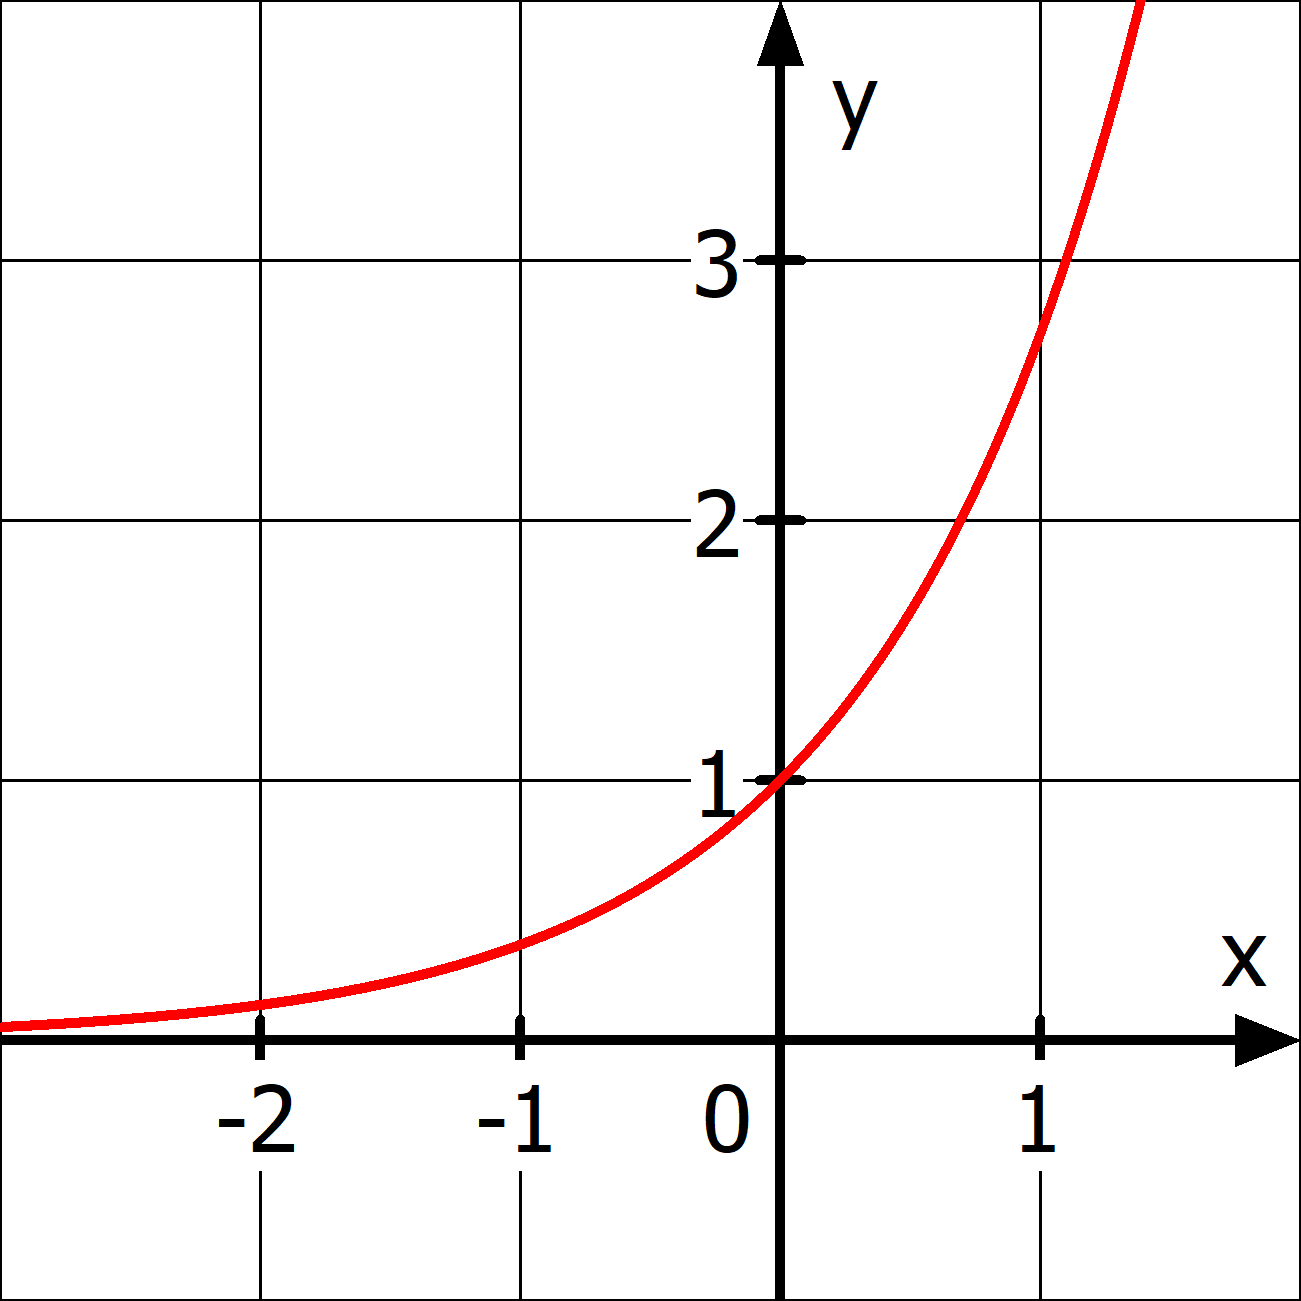
\includegraphics[width=.95\linewidth]{\eFkt/pics/e_x.png}
		\end{minipage}\\
		\centering \(a\) positiv, \(k\) positiv, z.B. \(f_1(x)=e^x\)
	\end{minipage}
	\begin{minipage}{0.49\textwidth}
		\begin{minipage}[t]{0.95\textwidth}
			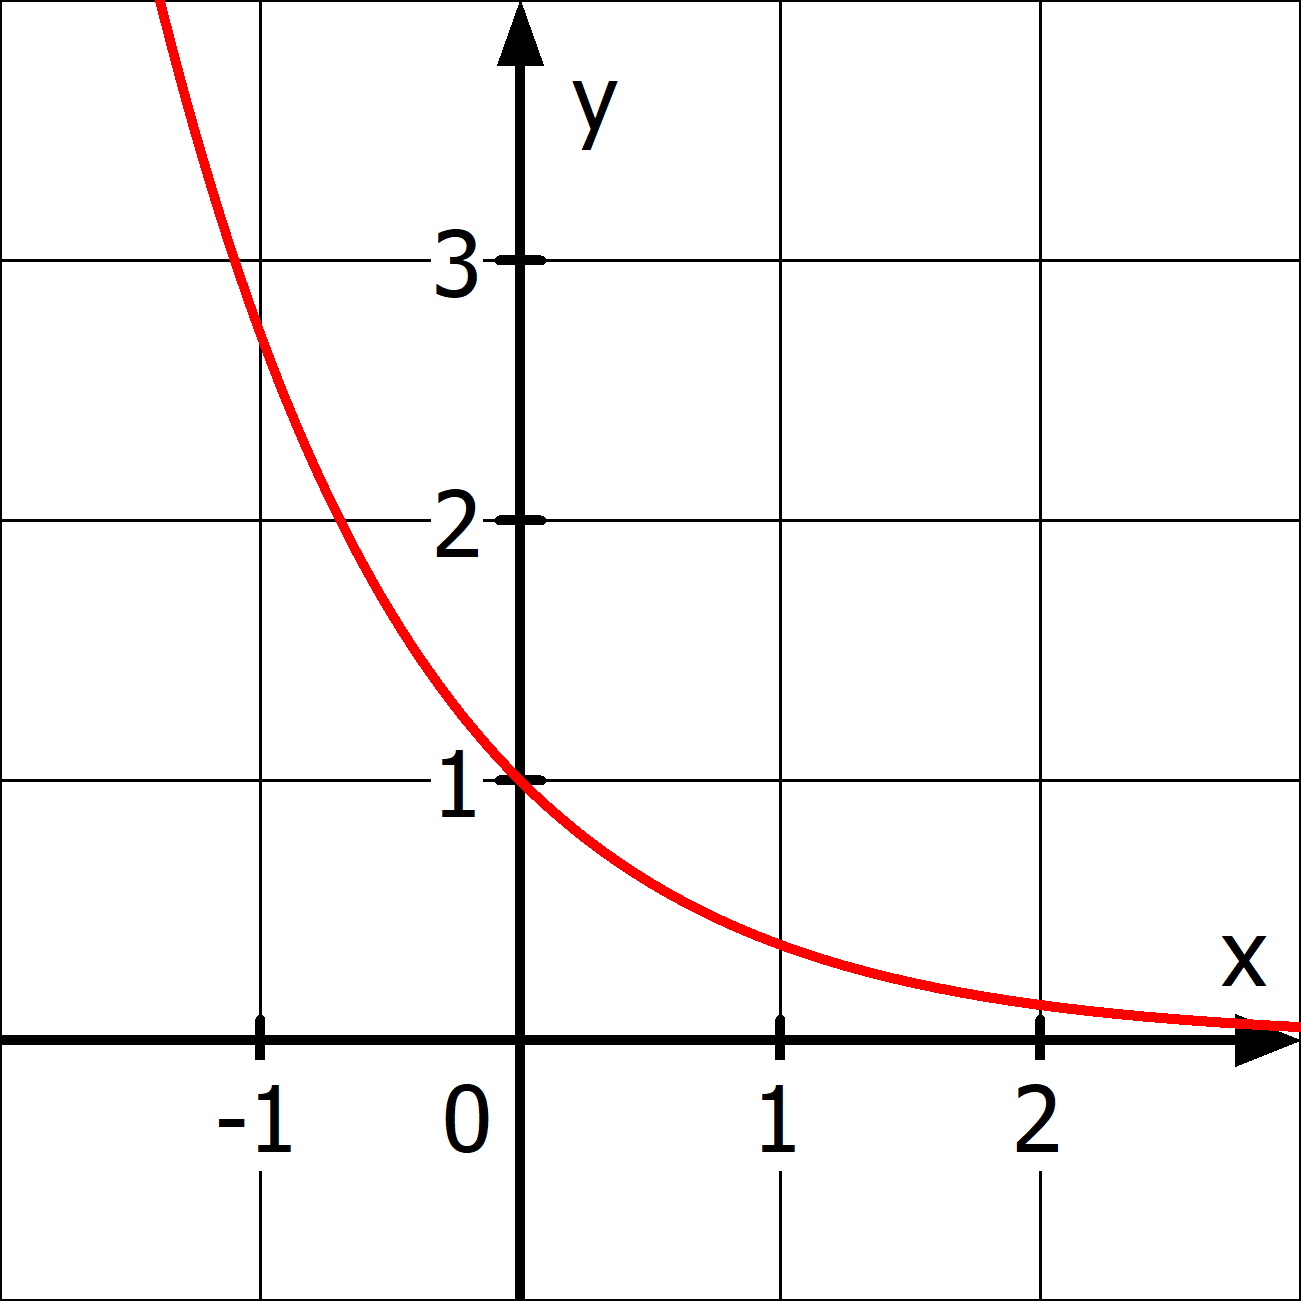
\includegraphics[width=.95\linewidth]{\eFkt/pics/e_minusx.png}
		\end{minipage}\\
		\centering \(a\) positiv, \(k\) negativ, z.B. \(f_2(x)=e^{-x}\)
	\end{minipage}
\end{minipage}\vspace{1cm}
\begin{minipage}{\textwidth}
	\begin{minipage}{0.49\textwidth}
		\begin{minipage}[t]{0.95\textwidth}
			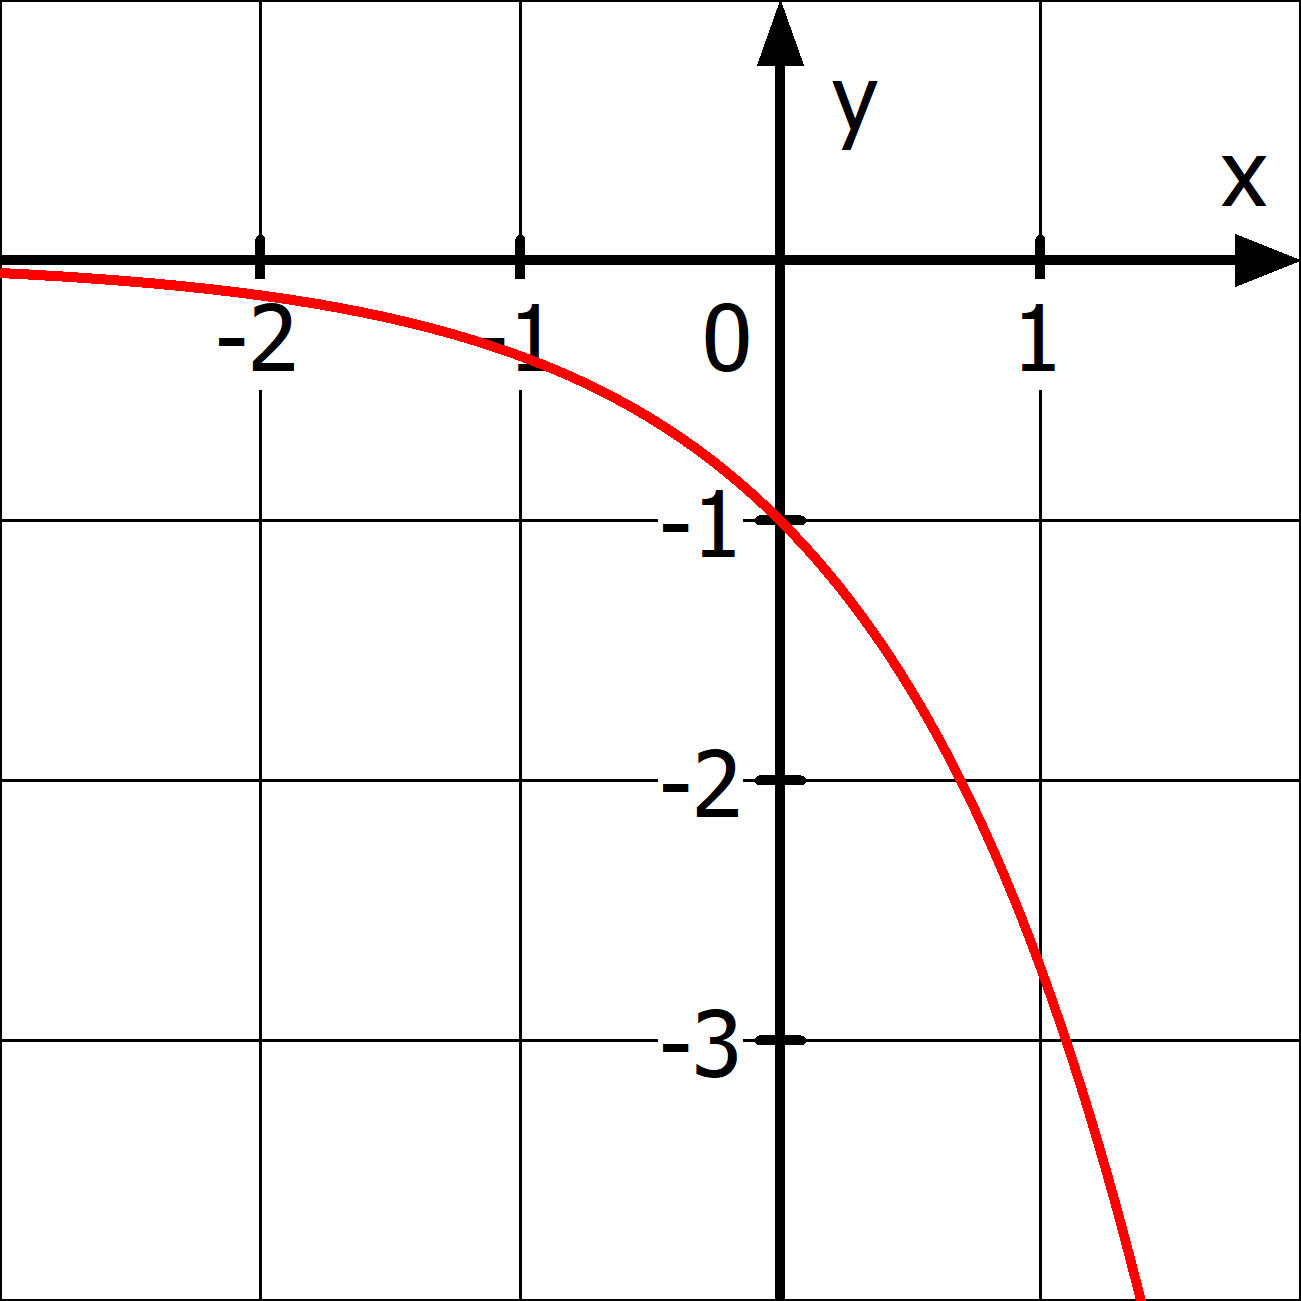
\includegraphics[width=.95\linewidth]{\eFkt/pics/minuse_x.png}
		\end{minipage}\\
		\centering \(a\) negativ, \(k\) positiv, z.B. \(f_3(x)=-e^x\)
	\end{minipage}
	\begin{minipage}{0.49\textwidth}
		\begin{minipage}[t]{0.95\textwidth}
			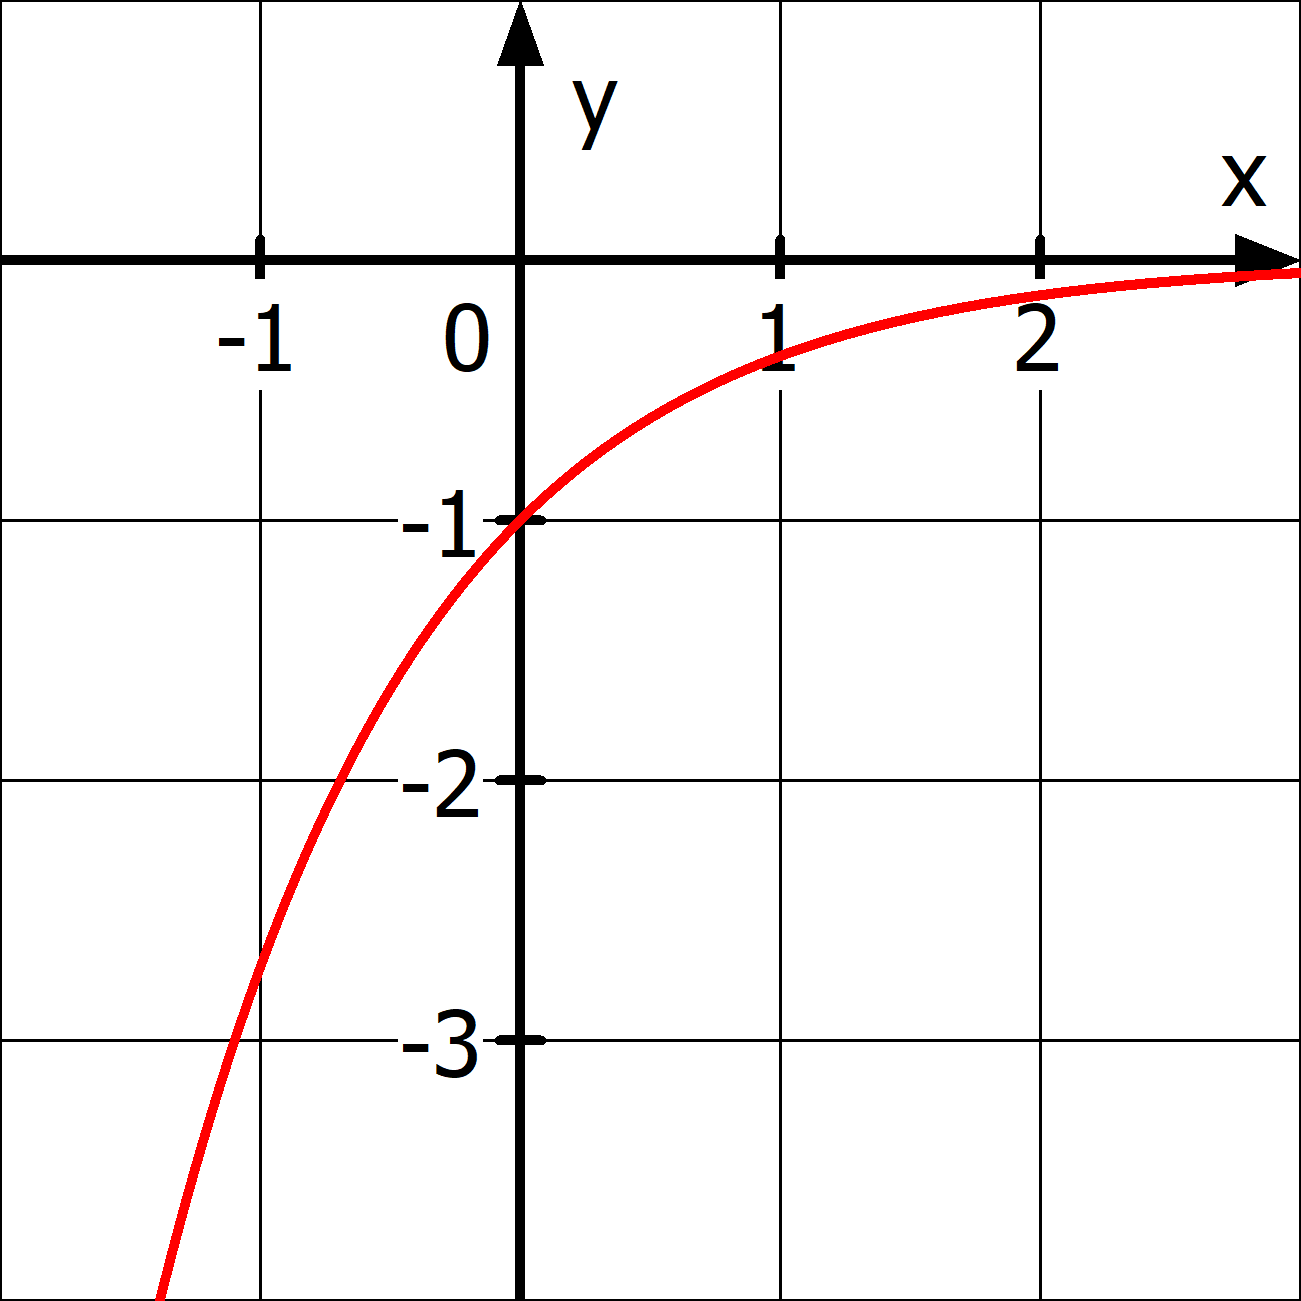
\includegraphics[width=.95\linewidth]{\eFkt/pics/minuse_minusx.png}
		\end{minipage}\\
		\centering \(a\) negativ, \(k\) negativ, z.B. \(f_4(x)=-e^{-x}\)
	\end{minipage}
\end{minipage}
\begin{tcolorbox}Wichtiger Funktionswert von \(e^x\):
	\[\bm{e^0=\textcolor{loestc}{1}}\]
\end{tcolorbox}
\newpage
%%%%%%%%%%%%%%%%%%%%%%%%%%%%%%%%%%%%%%%%%%%%%%%%%%%%%%%%%%%%%%%%%%%%%%%%%%%%%%%%%%%%%%%%%%%%%%%%%%%%%%
\cohead{\Large\textbf{Begriffe}}
Zur Einführung der neuen Begriffe Asymptote und Monotonie betrachten wir als Beispiel\\ \(f(x)=e^{\ln(2)\cdot x}=2^x\):\vspace{0.5cm}\\
\begin{minipage}{\textwidth}
	\begin{minipage}{0.55\textwidth}
		\begin{tcolorbox}
			\textbf{Asymptote}\\
			\textcolor{loestc}{Eine Asymptote einer Funktion ist eine Gerade, an die sich die Funktion beliebig nahe annähert, d.h. der Abstand zw. der Funktion und der Geraden wird beliebig klein. Im Beispiel halbiert man den Funktionswert immer wenn man einen Schritt nach links macht. Die Funktionswerte gehen also immer näher an die Null heran. Die Asymptote ist die x-Achse bzw. \(y=0\)}\vspace{2.7cm}
		\end{tcolorbox}
	\end{minipage}
	\begin{minipage}{0.44\textwidth}
		\begin{minipage}[t]{0.95\textwidth}
			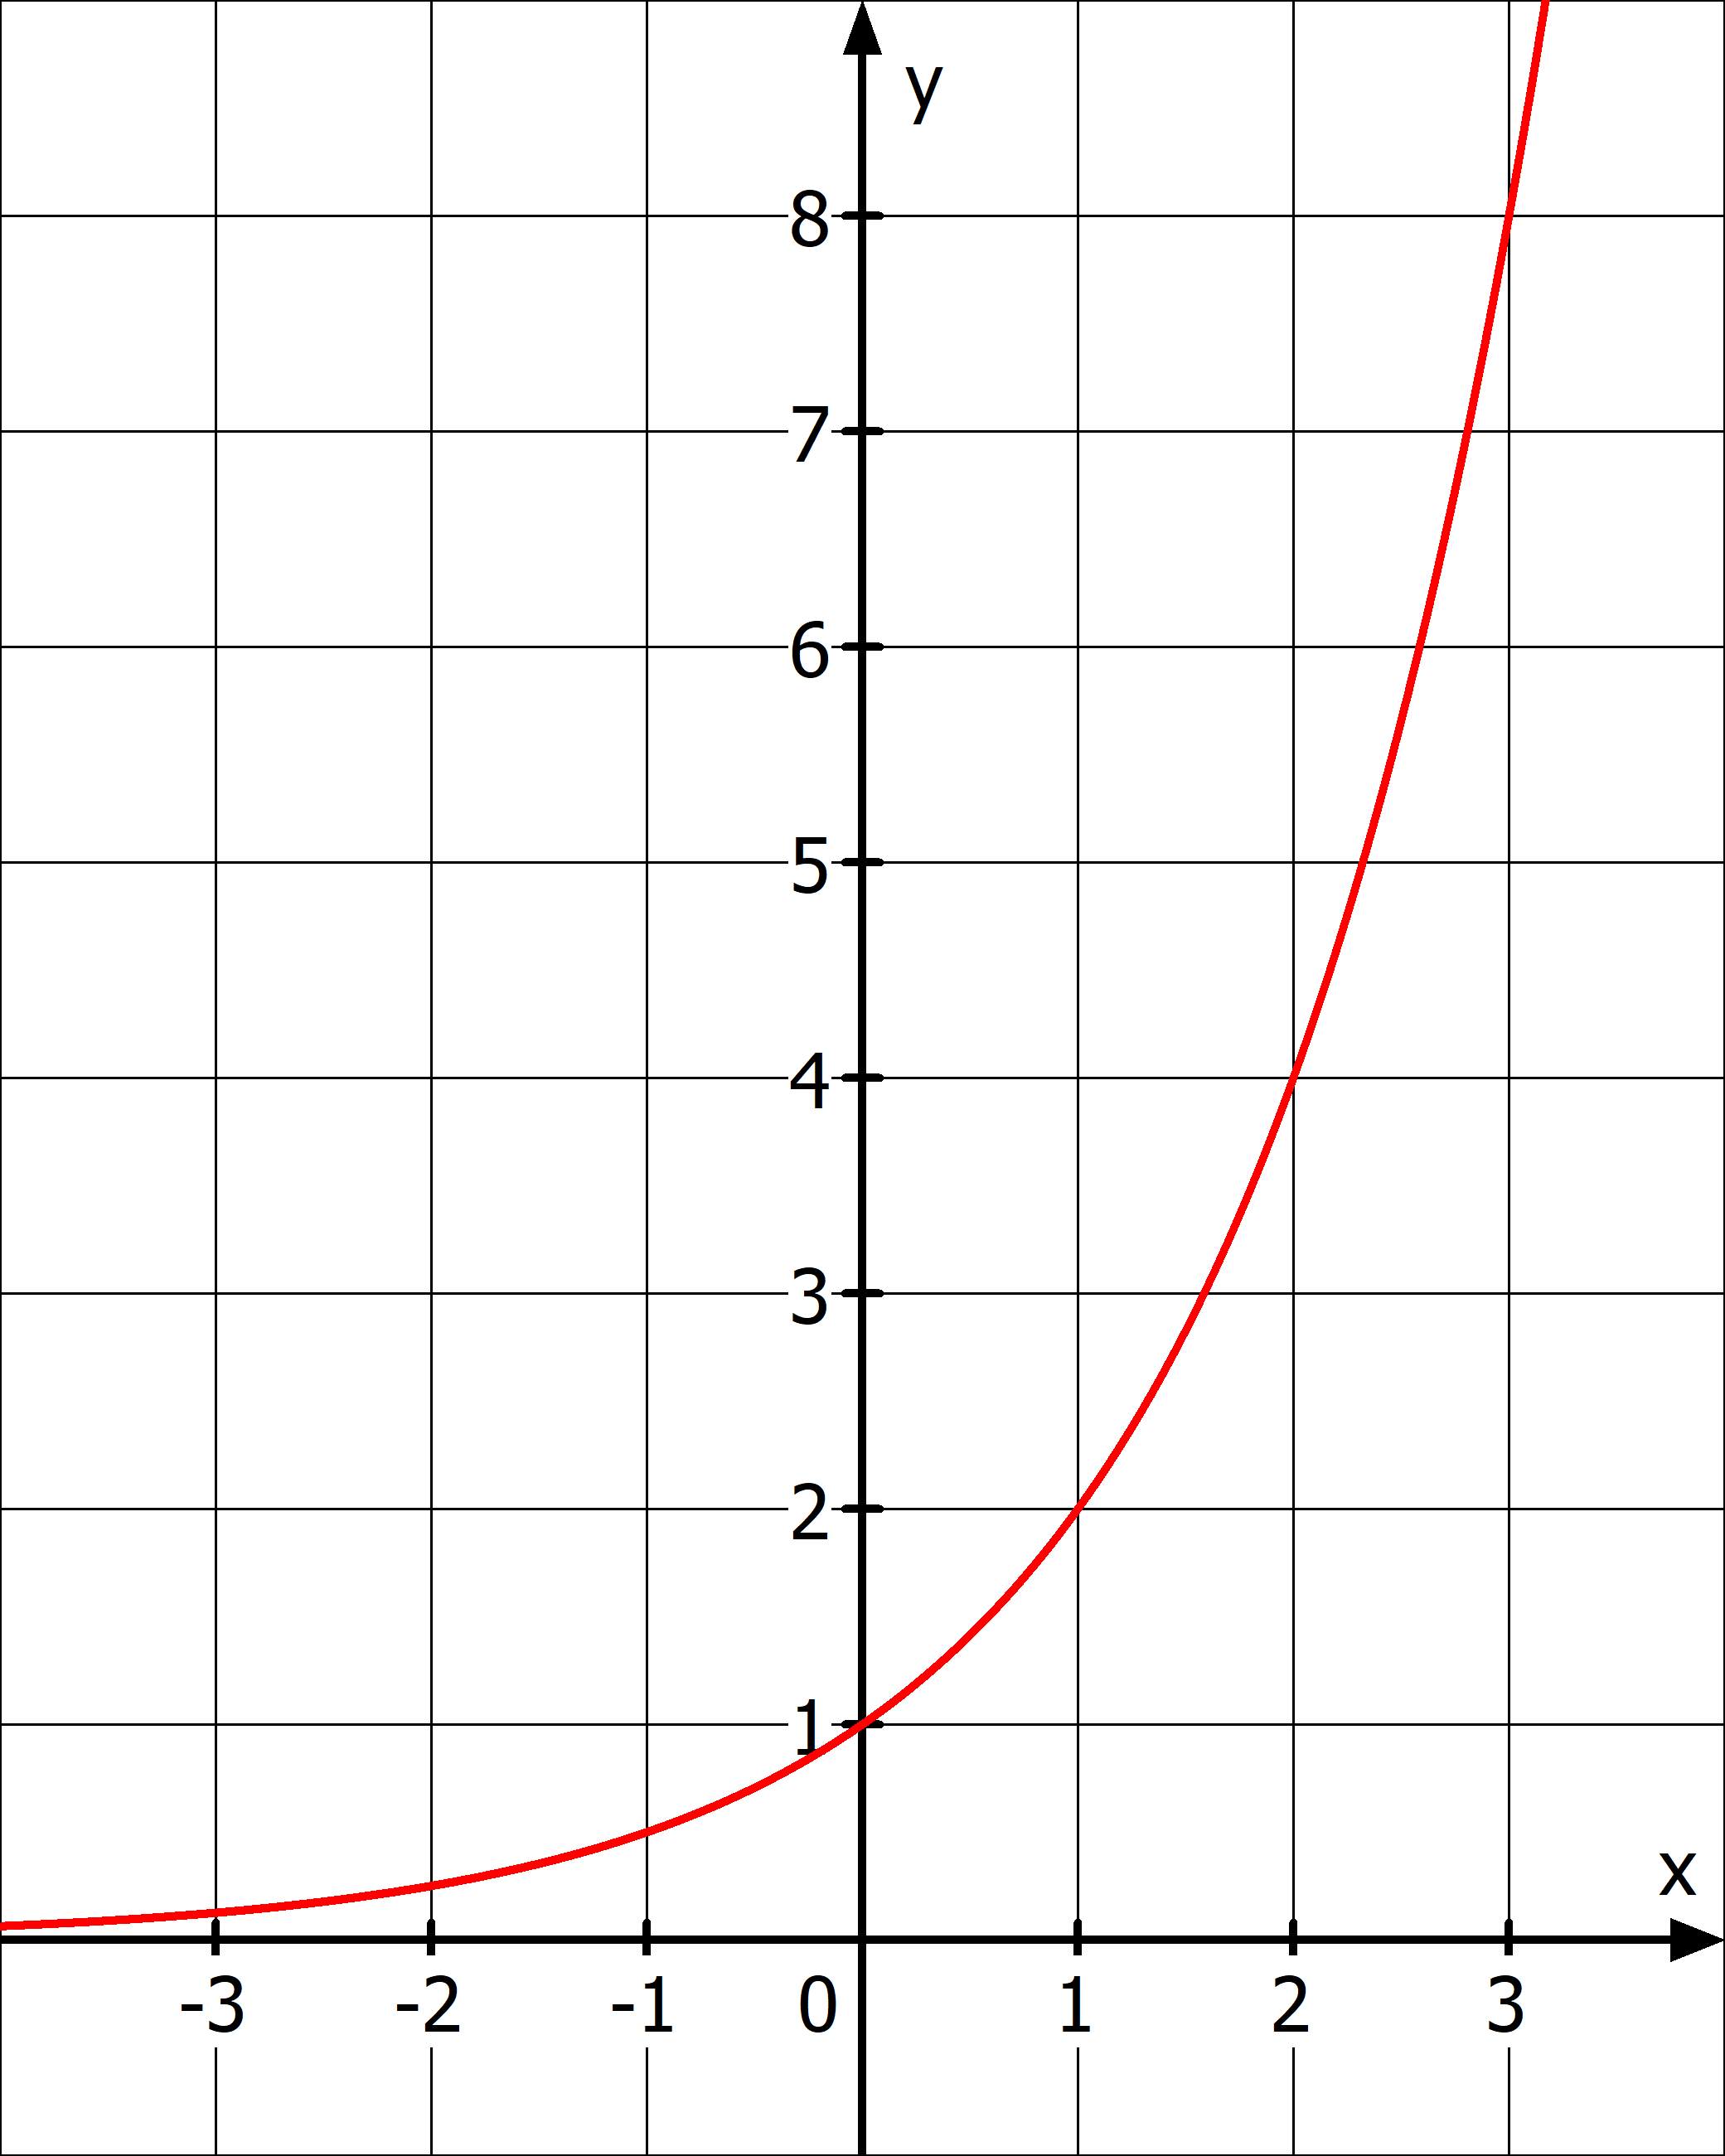
\includegraphics[width=.95\linewidth]{\eFkt/pics/2hochx.png}
		\end{minipage}
	\end{minipage}
\end{minipage}\\
\begin{tcolorbox}
	\textbf{Verhalten für \(x\rightarrow \pm\infty\)}
	\textcolor{loestc}{
		\begin{align*}
			f(x)&\xrightarrow{\hphantom{\ }x\to-\infty\hphantom{\ }}0\\
			f(x)&\xrightarrow{\hphantom{\ }x\to\infty\hphantom{\ }}\infty
	\end{align*}}
\end{tcolorbox}
\begin{tcolorbox}
	\textbf{Monotonie}\\
	\textcolor{loestc}{
		Wachsen die Funkionswerte bzw. y-Werte mit wachsenden x-Werten, so ist die Funktion monoton wachsend. Werden die Funktionswerte mit wachsenden x-Werten immer kleiner, so ist die Funktion Monoton fallend.\\
		Das Beispiel ist also monoton wachsend, da man von links nach rechts immer weiter nach oben geht. (Die Funktionswerte verdoppeln sich mit jedem Schritt nach rechts.)\vspace{3cm}}
\end{tcolorbox}
\newpage
%%%%%%%%%%%%%%%%%%%%%%%%%%%%%%%%%%%%%%%%%%%%%%%%%%%%%%%%%%%%%%%%%%%%%%%%%%%%%%%%%%%%%%%%%%%%%%%%%%%%%%%%%%%%%%%%%%%%%
\begin{Exercise}[title={Bestimme den y-Achsenabschnitt, skizziere das Schaubild, gib die Asymptote, das Verhalten für \(x\rightarrow \pm\infty\) und die Monotonie an}, label=eFktA1]\\
	\begin{minipage}{\textwidth}
		\begin{minipage}{0.49\textwidth}
			\begin{enumerate}[label=\alph*)]
				\item \(f(x)=e^{2x}\)
				\item \(f(x)=-3e^{\frac{1}{2}x}\)
				\item \(f(x)=-4e^{-2x}\)
				\item \(f(x)=2e^{-7x}\)
				\item \(f(x)=-\frac{5}{3}e^{x}\)
				\item \(f(x)=8e^{-3x}\)
				\item \(f(x)=-3e^{-\frac{9}{8}x}\)
				\item \(f(x)=\frac{3}{5}e^{0,2x}\)
				\item \(f(x)=-0,5e^{-3,5x}\)
				\item \(f(x)=-8e^{\frac{1}{10}x}\)
				\item \(f(x)=2e^{-2x}\)
				\item \(f(x)=-4e^{-7x}\)
				\item \(f(x)=-\frac{5}{7}e^{x}\)
			\end{enumerate}
		\end{minipage}
		\begin{minipage}{0.49\textwidth}
			\begin{enumerate}[label=\alph*)]
				\setcounter{enumi}{13}
				\item \(f(x)=6e^{-4x}\)
				\item \(f(x)=-2e^{-8x}\)
				\item \(f(x)=5,3e^{0,2x}\)
				\item \(f(x)=-\frac{1}{4}e^{-\frac{2}{3}x}\)
				\item \(f(x)=-2e^{0,2x}\)
				\item \(f(x)=1,8e^{-4x}\)
				\item \(f(x)=5e^{7x}\)
				\item \(f(x)=-\frac{8}{3}e^{\frac{3}{8}x}\)
				\item \(f(x)=-0,1e^{-0,3x}\)
				\item \(f(x)=10e^{-4x}\)
				\item \(f(x)=-5e^{6x}\)
				\item \(f(x)=-0,9e^{-1,1x}\)
				\item \(f(x)=\frac{11}{6}e^{\frac{8}{7}x}\)
			\end{enumerate}
		\end{minipage}
	\end{minipage}
\end{Exercise}
\newpage
%%%%%%%%%%%%%%%%%%%%%%%%%%%%%%%%%%%%%%%%%
\begin{Answer}[ref=eFktA1]\\
	%%%%% a bis f
	\begin{minipage}{\textwidth}
		\begin{minipage}[t]{0.49\textwidth}
			\begin{enumerate}[label=\alph*)]
				\item \(f(x)=e^{2x}\)\\
				Asymptote \(y=0\)\\
				y-Achsenabschnitt: \(f(0)=1\)\\
				Monoton wachsend\\
				\(f(x)\xrightarrow{\hphantom{\ }x\to-\infty\hphantom{\ }}0\)\\
				\(f(x)\xrightarrow{\hphantom{\ }x\to\infty\hphantom{\ }}\infty\)\\
				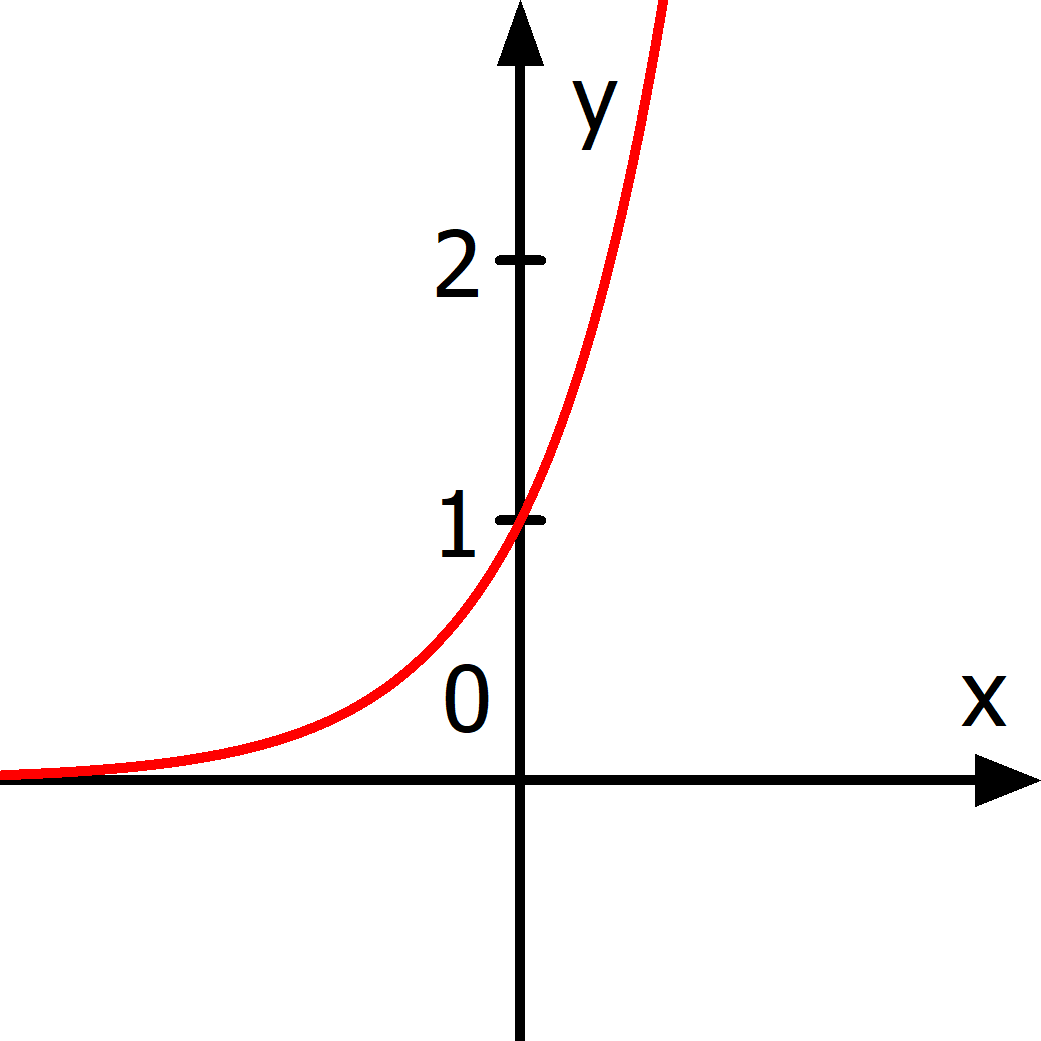
\includegraphics[width=.6\linewidth]{\eFkt/pics/A1a.png}
				\item \(f(x)=-3e^{\frac{1}{2}x}\)\\
				Asymptote \(y=0\)\\
				y-Achsenabschnitt: \(f(0)=-3\)\\
				Monoton fallend\\
				\(f(x)\xrightarrow{\hphantom{\ }x\to-\infty\hphantom{\ }}0\)\\
				\(f(x)\xrightarrow{\hphantom{\ }x\to\infty\hphantom{\ }}-\infty\)\\
				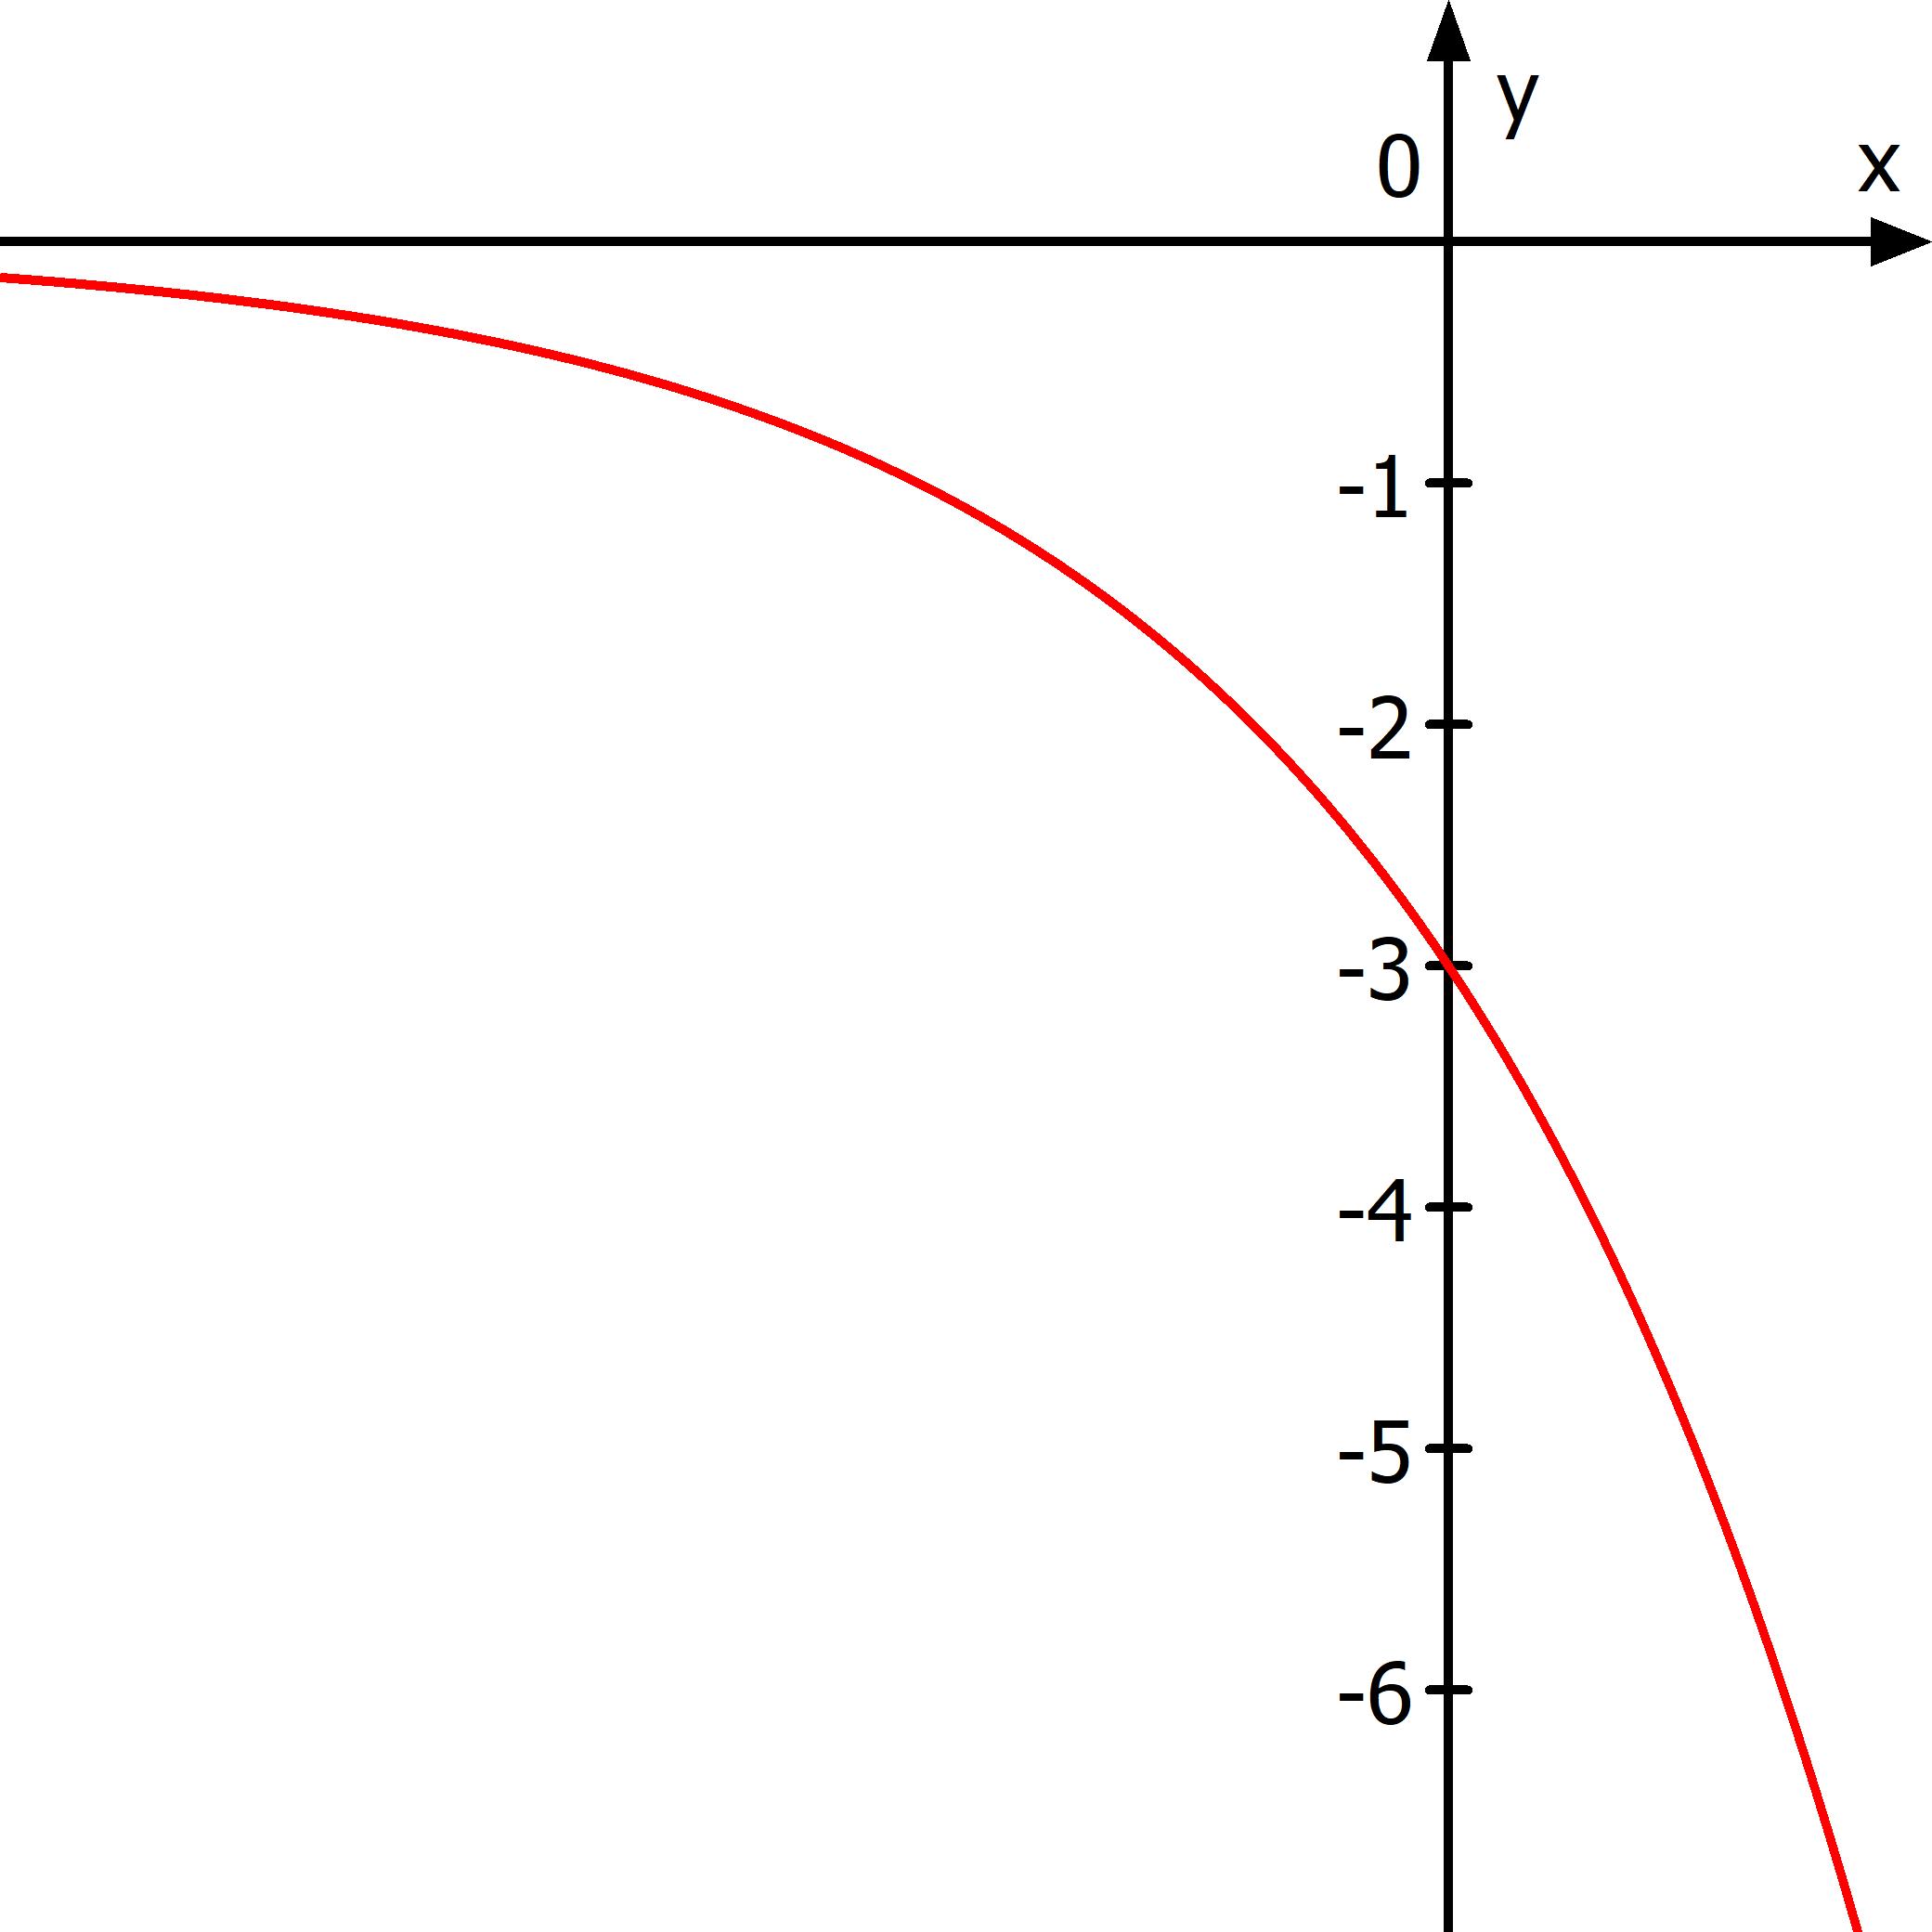
\includegraphics[width=.6\linewidth]{\eFkt/pics/A1b.png}
				\item \(f(x)=-4e^{-2x}\)\\
				Asymptote \(y=0\)\\
				y-Achsenabschnitt: \(f(0)=-4\)\\
				Monoton wachsend\\
				\(f(x)\xrightarrow{\hphantom{\ }x\to-\infty\hphantom{\ }}-\infty\)\\
				\(f(x)\xrightarrow{\hphantom{\ }x\to\infty\hphantom{\ }}0\)\\
				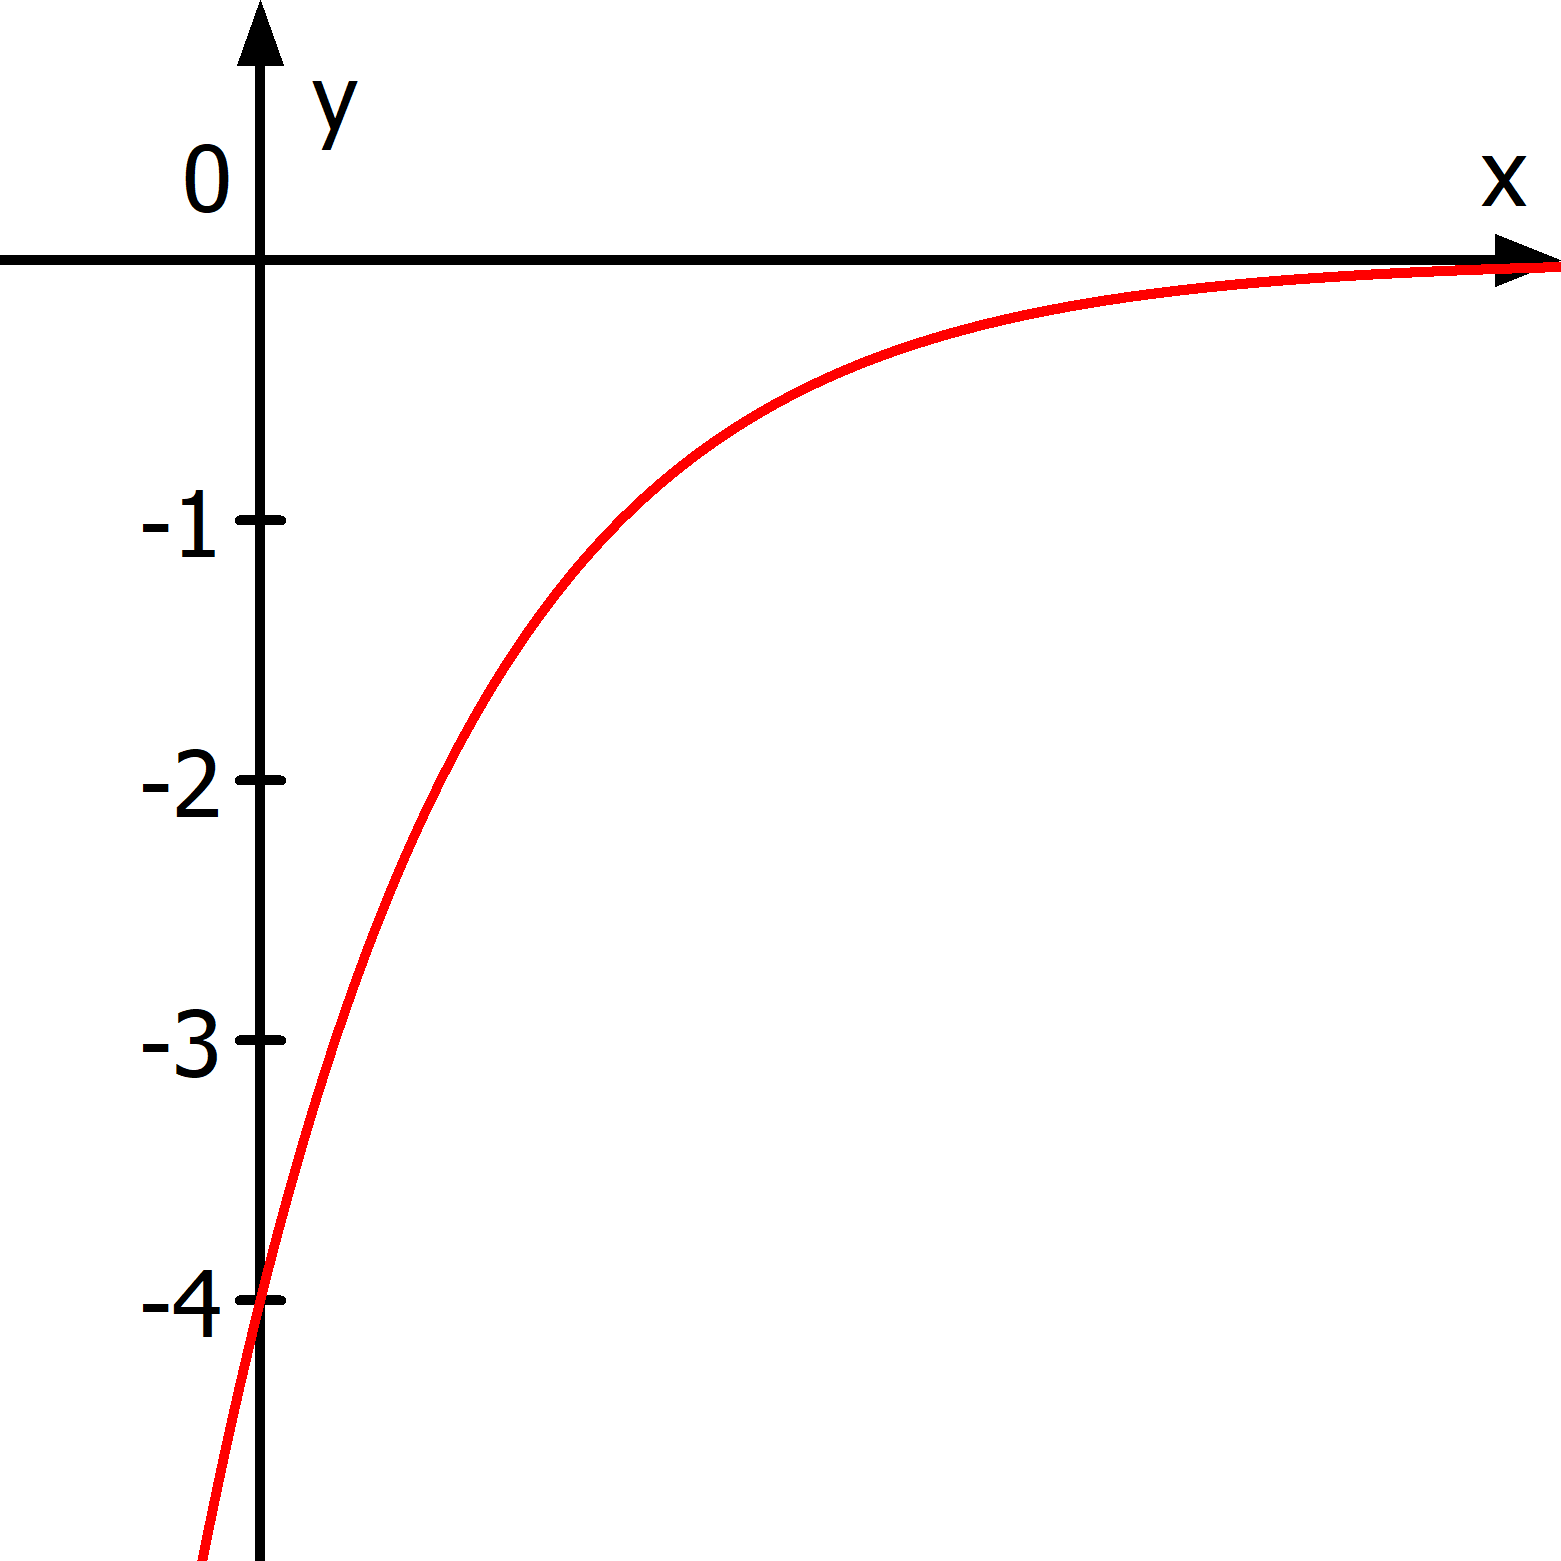
\includegraphics[width=.6\linewidth]{\eFkt/pics/A1c.png}
			\end{enumerate}
		\end{minipage}
		\begin{minipage}[t]{0.49\textwidth}
			\begin{enumerate}[label=\alph*)]
				\setcounter{enumi}{3}
				\item \(f(x)=2e^{-7x}\)\\
				Asymptote \(y=0\)\\
				y-Achsenabschnitt: \(f(0)=2\)\\
				Monoton fallend\\
				\(f(x)\xrightarrow{\hphantom{\ }x\to-\infty\hphantom{\ }}\infty\)\\
				\(f(x)\xrightarrow{\hphantom{\ }x\to\infty\hphantom{\ }}0\)\\
				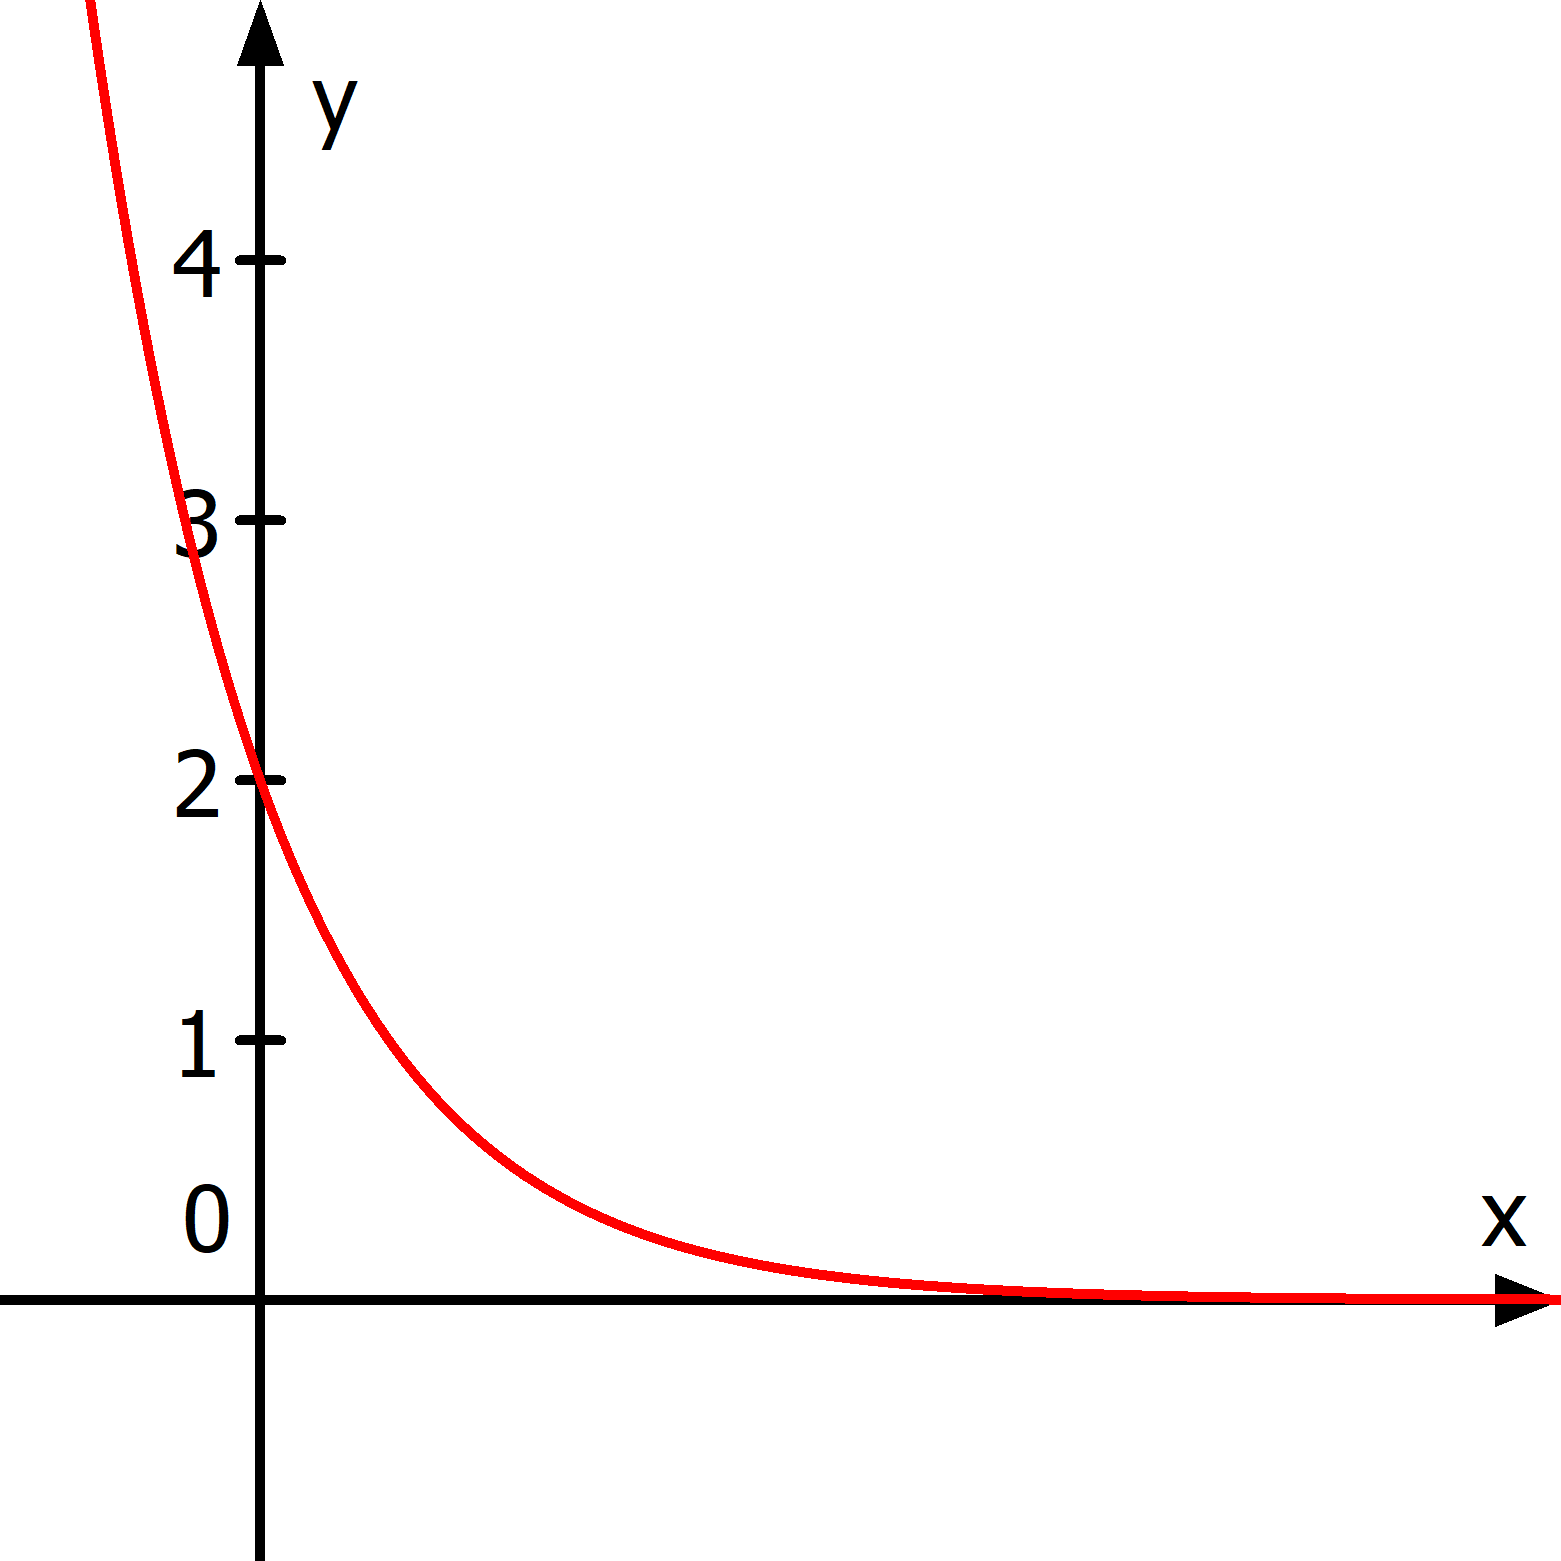
\includegraphics[width=.6\linewidth]{\eFkt/pics/A1d.png}
				\item \(f(x)=-\frac{5}{3}e^{x}\)\\
				Asymptote \(y=0\)\\
				y-Achsenabschnitt: \(f(0)=-\frac{5}{3}\)\\
				Monoton fallend\\
				\(f(x)\xrightarrow{\hphantom{\ }x\to-\infty\hphantom{\ }}0\)\\
				\(f(x)\xrightarrow{\hphantom{\ }x\to\infty\hphantom{\ }}-\infty\)\\
				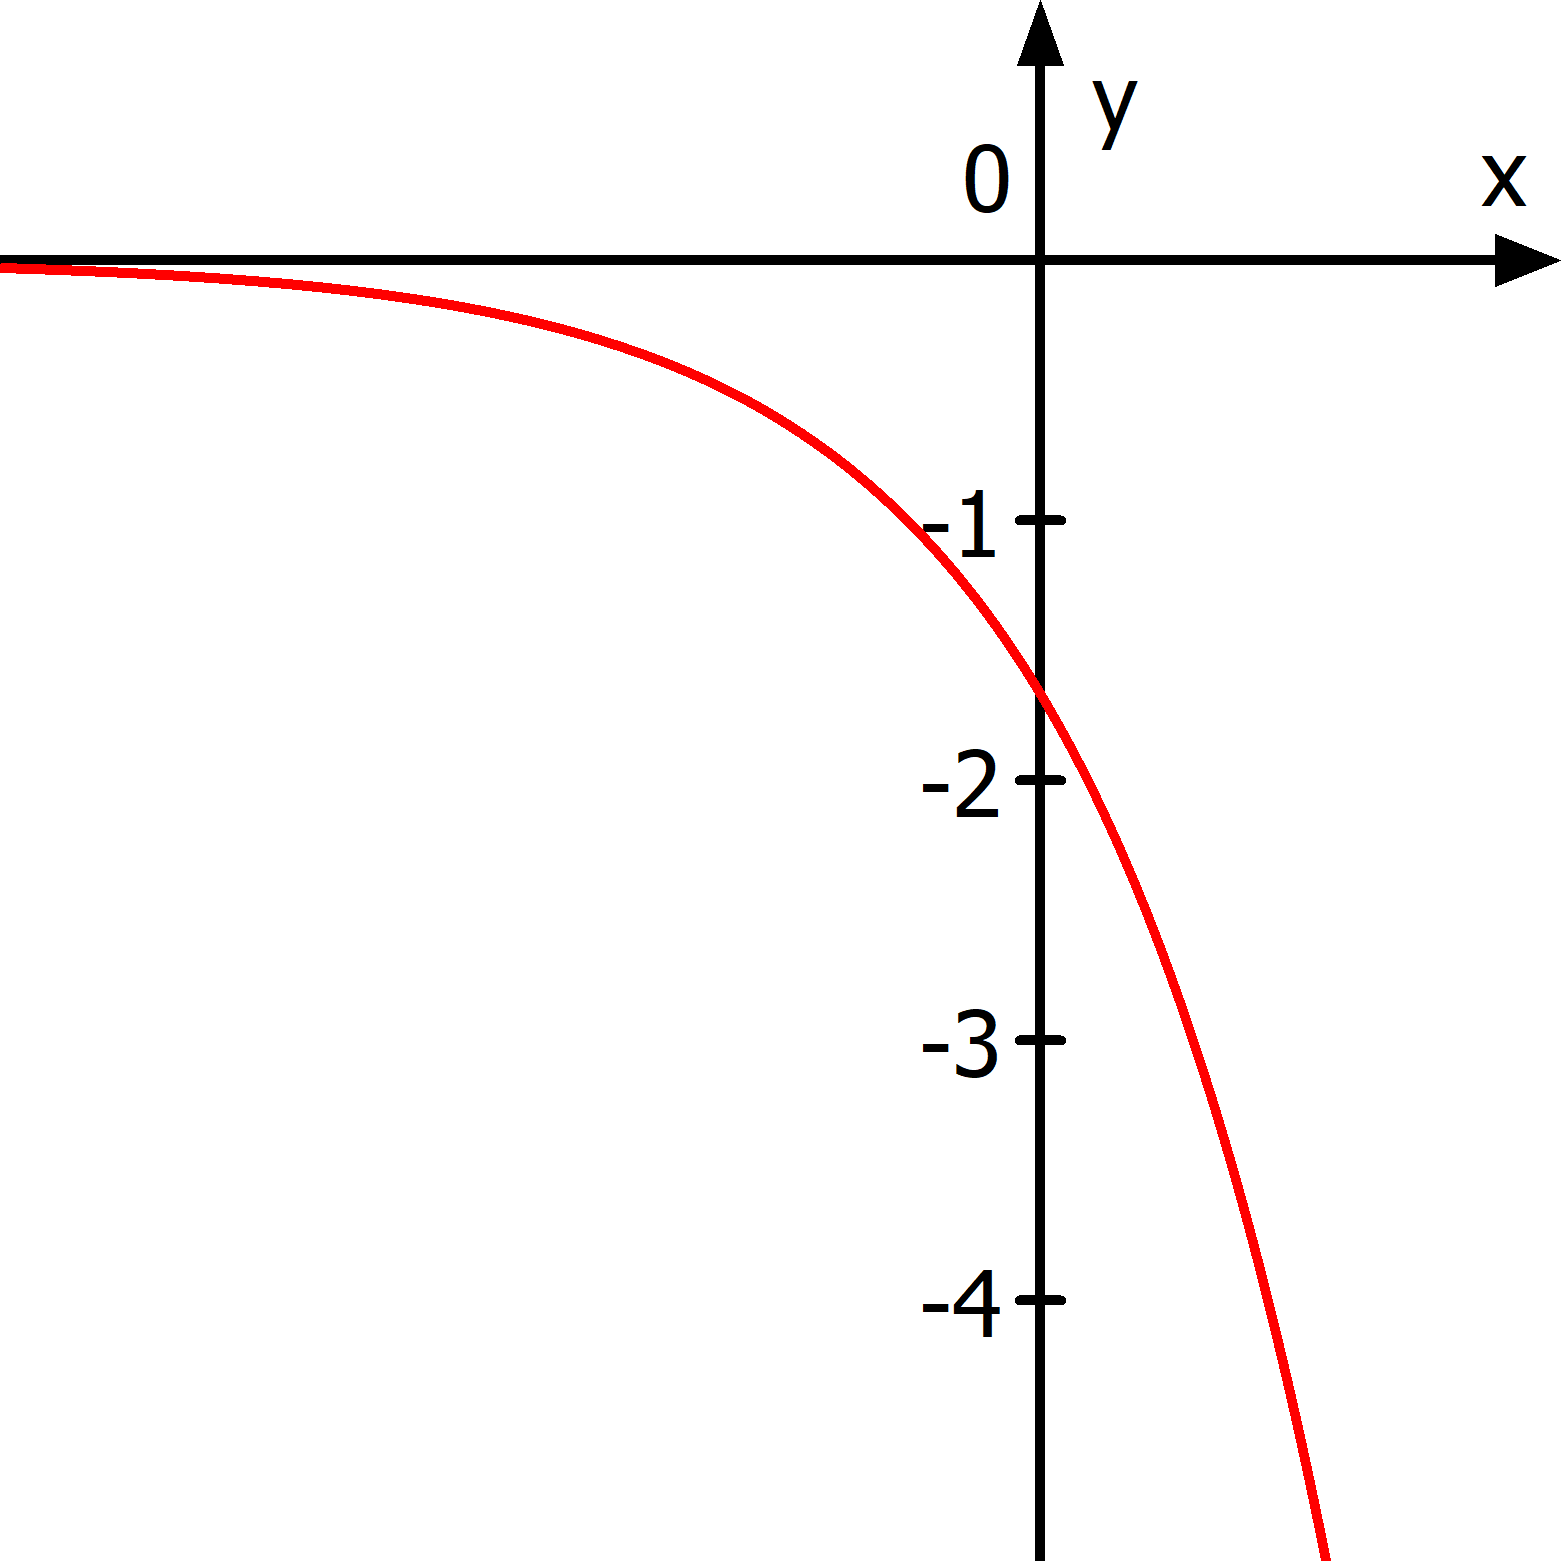
\includegraphics[width=.6\linewidth]{\eFkt/pics/A1e.png}
				\item \(f(x)=8e^{-3x}\)\\
				Asymptote \(y=0\)\\
				y-Achsenabschnitt: \(f(0)=8\)\\
				Monoton fallend\\
				\(f(x)\xrightarrow{\hphantom{\ }x\to-\infty\hphantom{\ }}\infty\)\\
				\(f(x)\xrightarrow{\hphantom{\ }x\to\infty\hphantom{\ }}0\)\\
				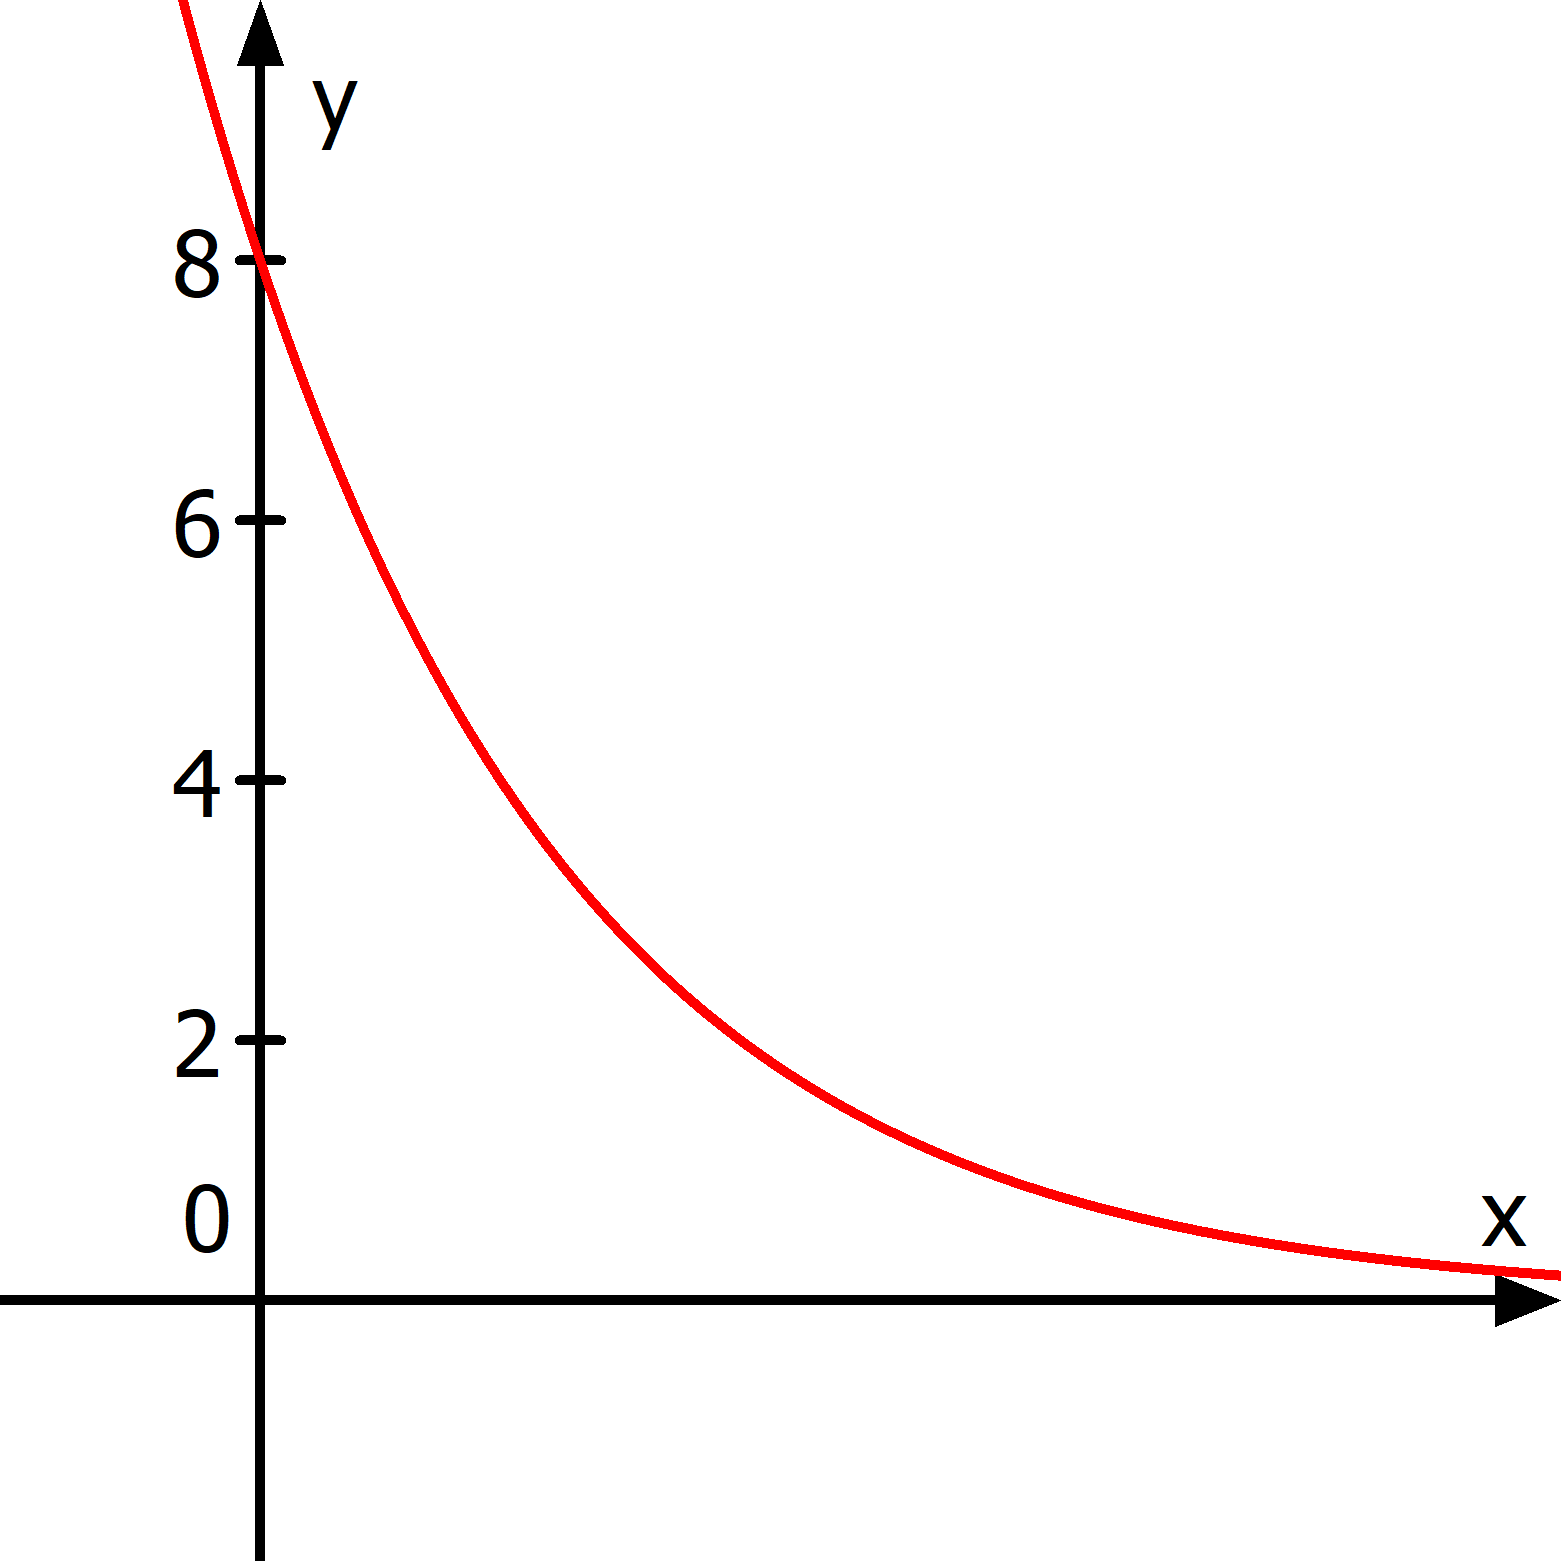
\includegraphics[width=.6\linewidth]{\eFkt/pics/A1f.png}
			\end{enumerate}
		\end{minipage}
	\end{minipage}\\
	%%%%% g bis l
	\begin{minipage}{\textwidth}
		\begin{minipage}[t]{0.49\textwidth}
			\begin{enumerate}[label=\alph*)]
				\setcounter{enumi}{6}
				\item \(f(x)=-3e^{-\frac{9}{8}x}\)\\
				Asymptote \(y=0\)\\
				y-Achsenabschnitt: \(f(0)=-3\)\\
				Monoton wachsend\\
				\(f(x)\xrightarrow{\hphantom{\ }x\to-\infty\hphantom{\ }}-\infty\)\\
				\(f(x)\xrightarrow{\hphantom{\ }x\to\infty\hphantom{\ }}0\)\\
				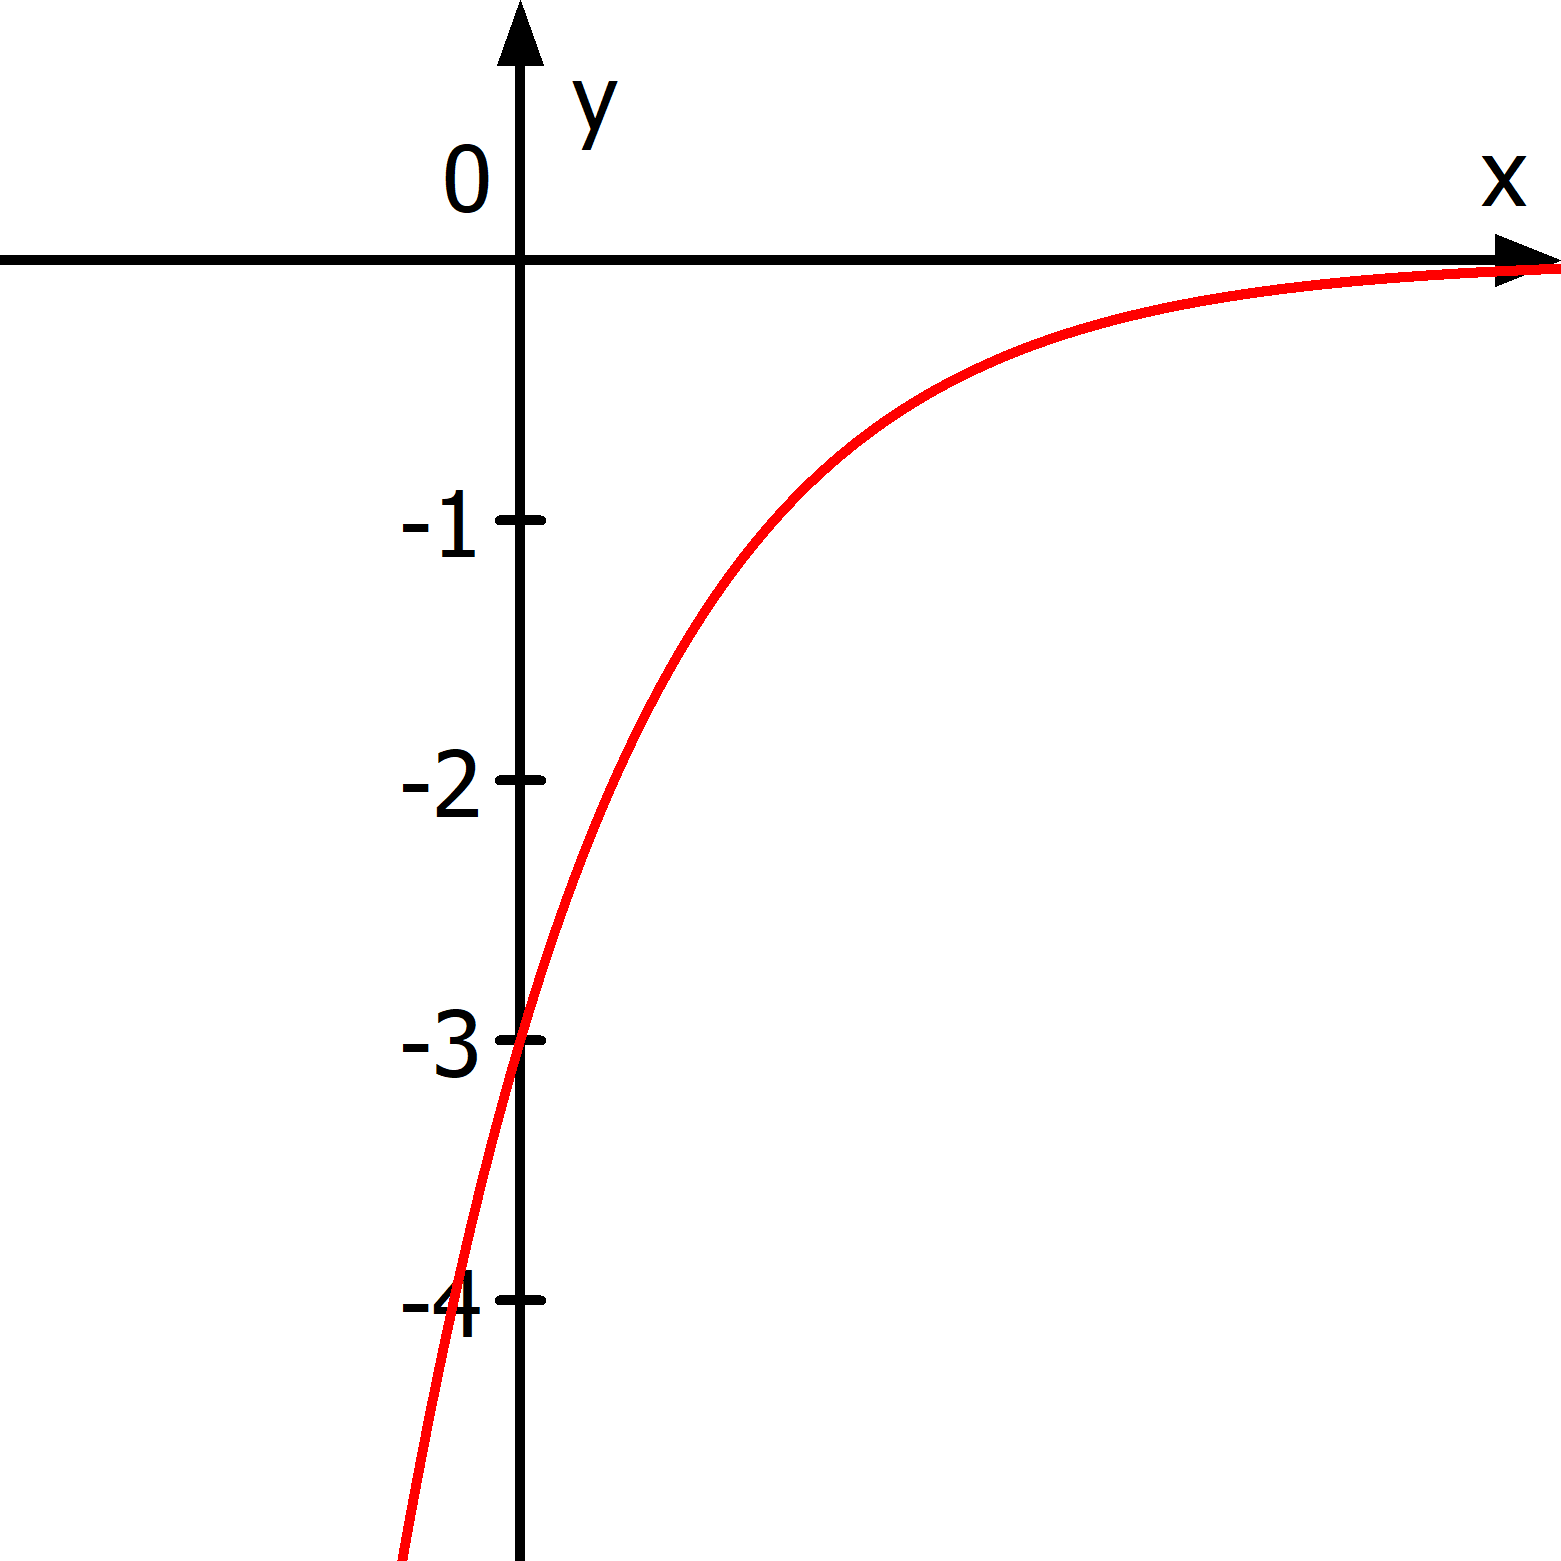
\includegraphics[width=.6\linewidth]{\eFkt/pics/A1g.png}
				\item \(f(x)=\frac{3}{5}e^{0,2x}\)\\
				Asymptote \(y=0\)\\
				y-Achsenabschnitt: \(f(0)=\frac{3}{5}\)\\
				Monoton wachsend\\
				\(f(x)\xrightarrow{\hphantom{\ }x\to-\infty\hphantom{\ }}0\)\\
				\(f(x)\xrightarrow{\hphantom{\ }x\to\infty\hphantom{\ }}\infty\)\\
				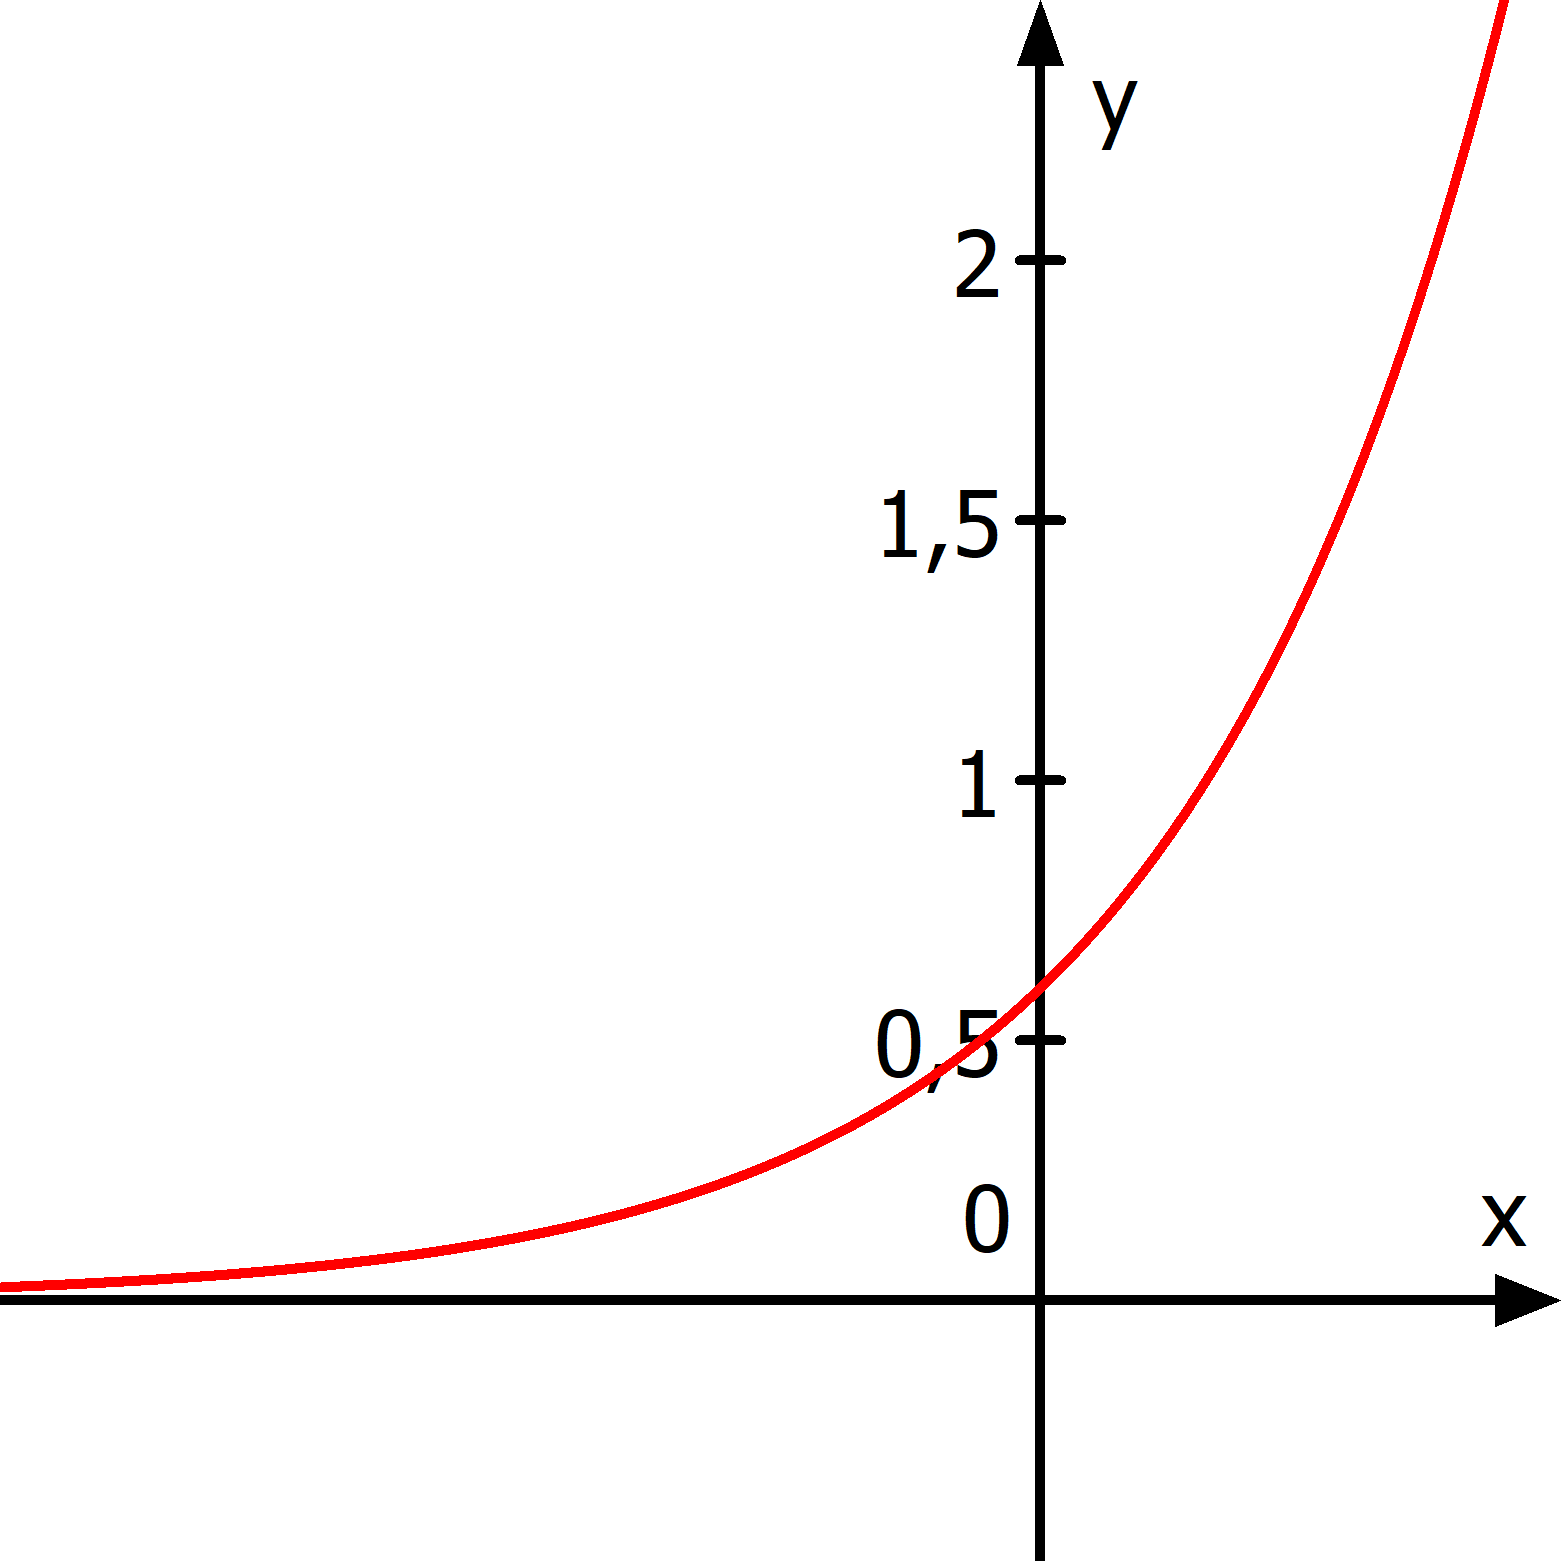
\includegraphics[width=.6\linewidth]{\eFkt/pics/A1h.png}
				\item \(f(x)=-0,5e^{-3,5x}\)\\
				Asymptote \(y=0\)\\
				y-Achsenabschnitt: \(f(0)=-0,5\)\\
				Monoton wachsend\\
				\(f(x)\xrightarrow{\hphantom{\ }x\to-\infty\hphantom{\ }}-\infty\)\\
				\(f(x)\xrightarrow{\hphantom{\ }x\to\infty\hphantom{\ }}0\)\\
				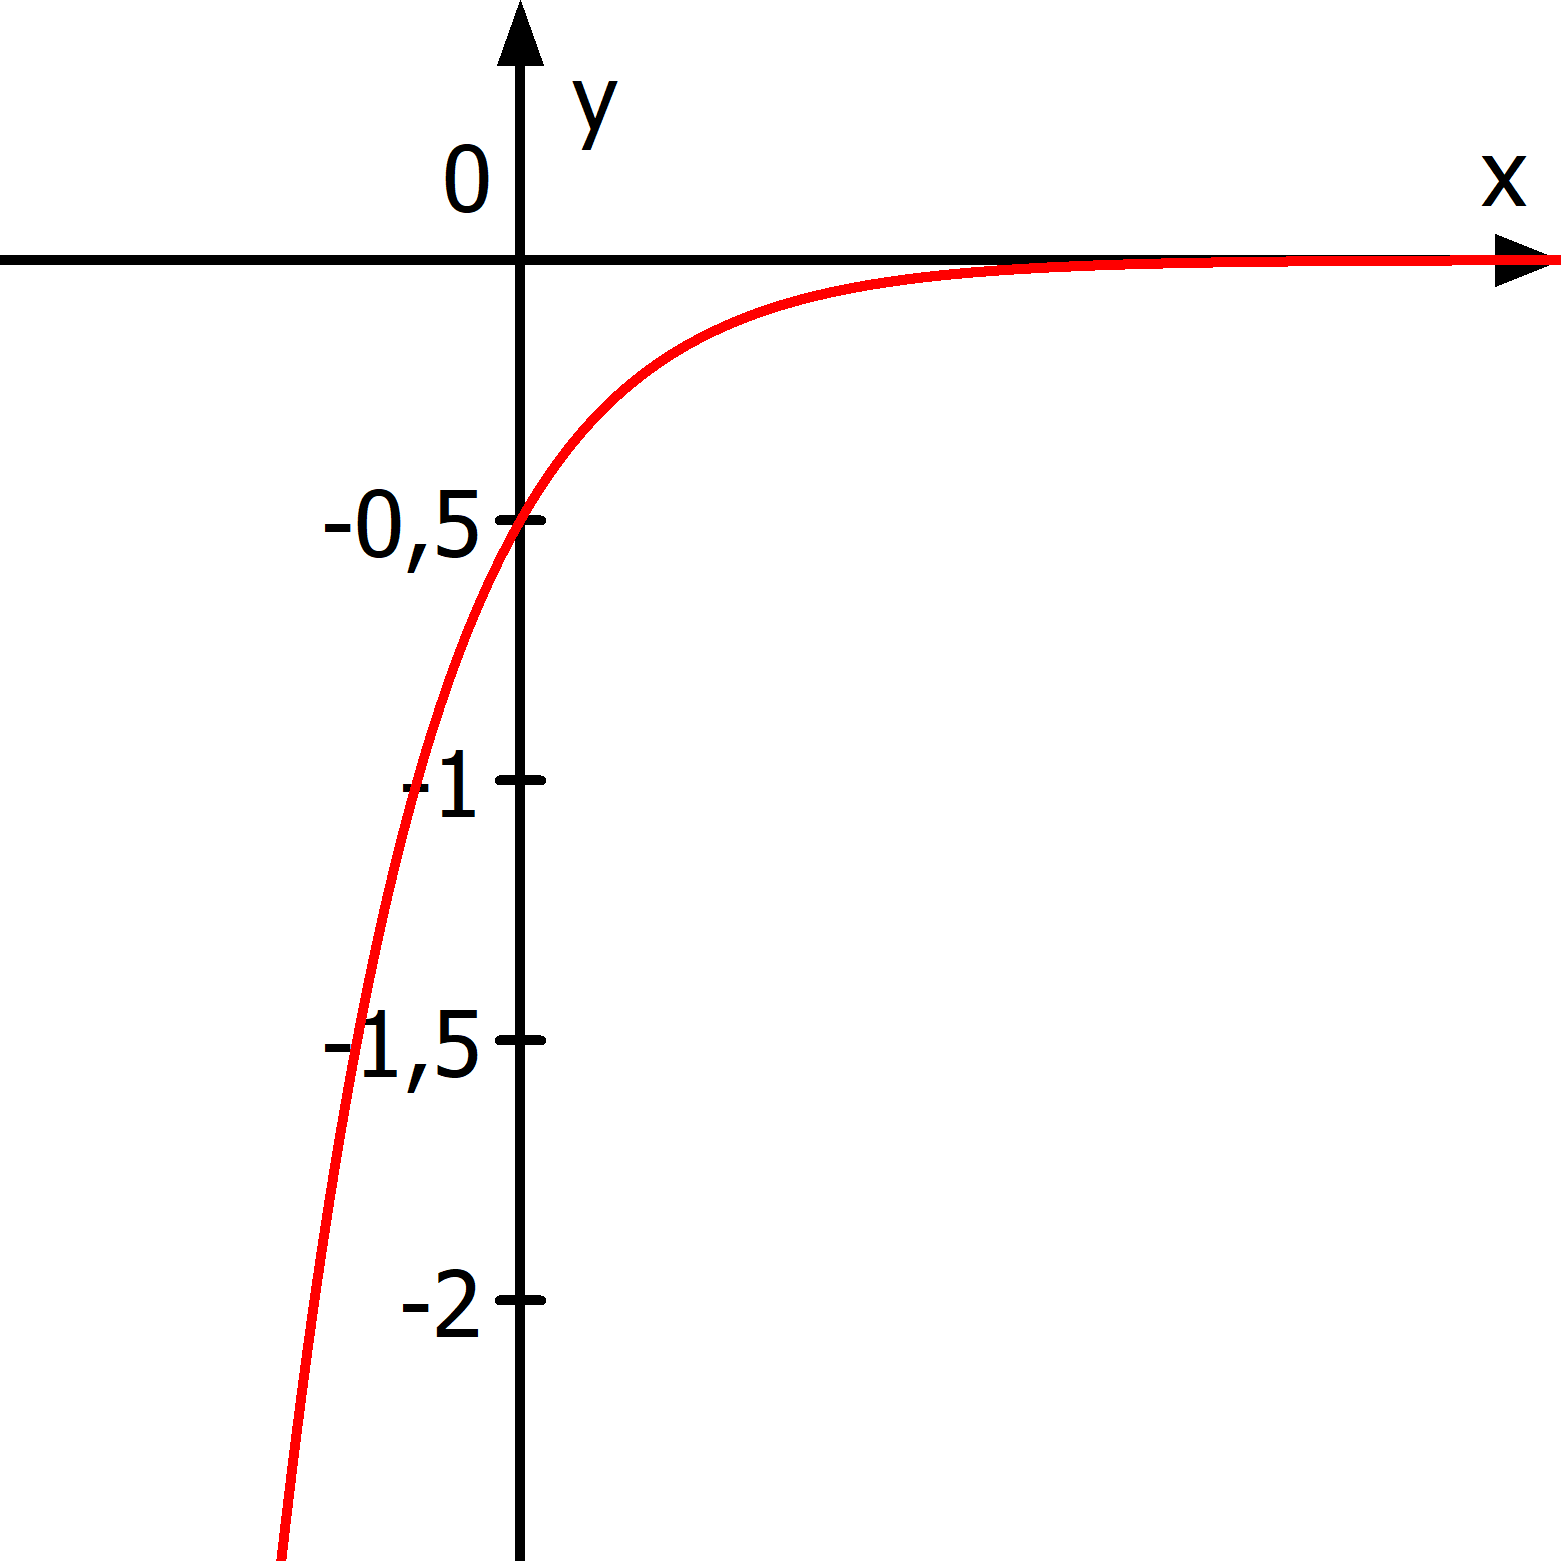
\includegraphics[width=.6\linewidth]{\eFkt/pics/A1i.png}
			\end{enumerate}
		\end{minipage}
		\begin{minipage}[t]{0.49\textwidth}
			\begin{enumerate}[label=\alph*)]
				\setcounter{enumi}{9}
				\item \(f(x)=-8e^{\frac{1}{10}x}\)\\
				Asymptote \(y=0\)\\
				y-Achsenabschnitt: \(f(0)=-8\)\\
				Monoton fallend\\
				\(f(x)\xrightarrow{\hphantom{\ }x\to-\infty\hphantom{\ }}0\)\\
				\(f(x)\xrightarrow{\hphantom{\ }x\to\infty\hphantom{\ }}-\infty\)\\
				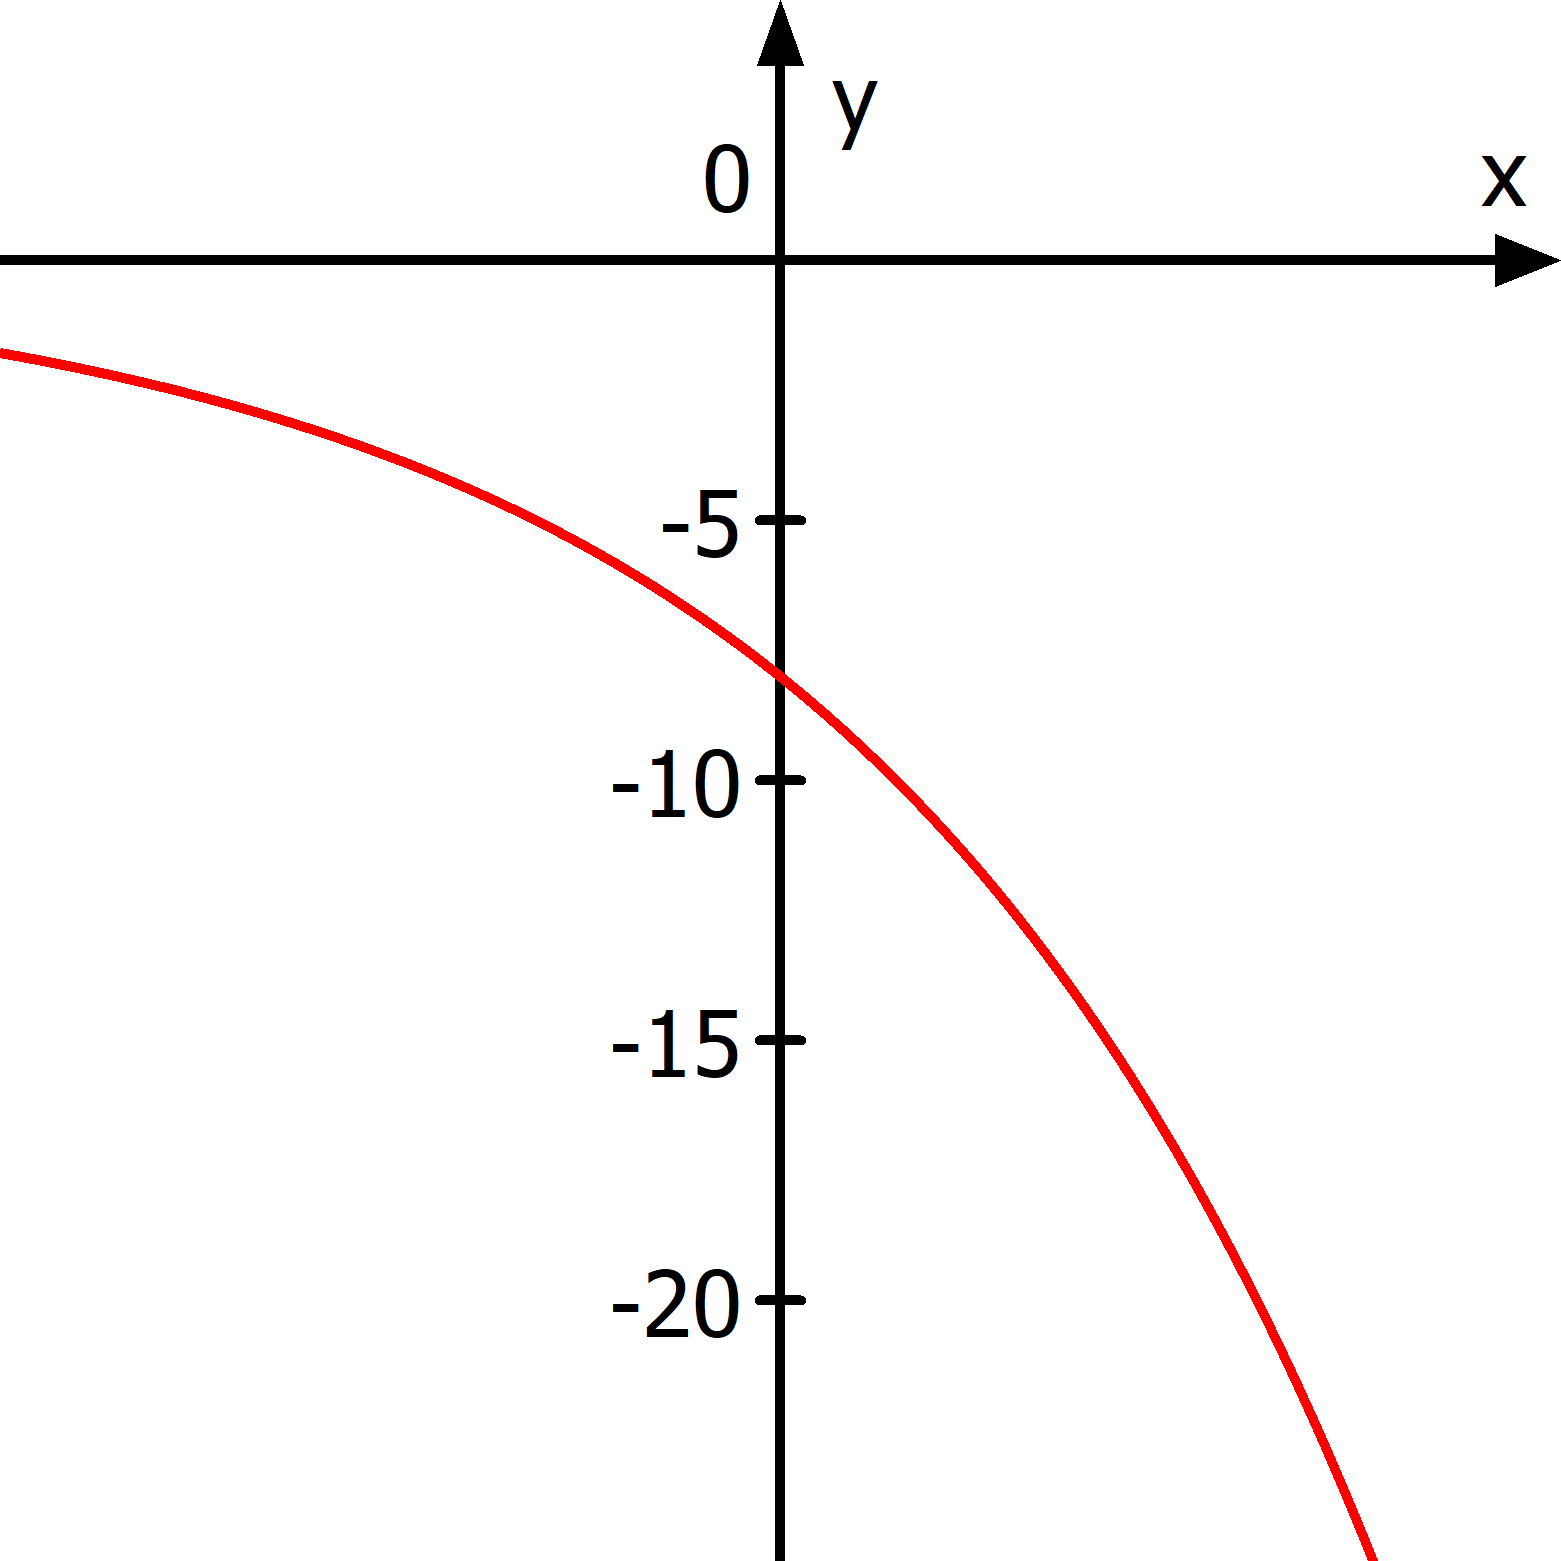
\includegraphics[width=.6\linewidth]{\eFkt/pics/A1j.png}
				\item \(f(x)=2e^{-2x}\)\\
				Asymptote \(y=0\)\\
				y-Achsenabschnitt: \(f(0)=2\)\\
				Monoton fallend\\
				\(f(x)\xrightarrow{\hphantom{\ }x\to-\infty\hphantom{\ }}\infty\)\\
				\(f(x)\xrightarrow{\hphantom{\ }x\to\infty\hphantom{\ }}0\)\\
				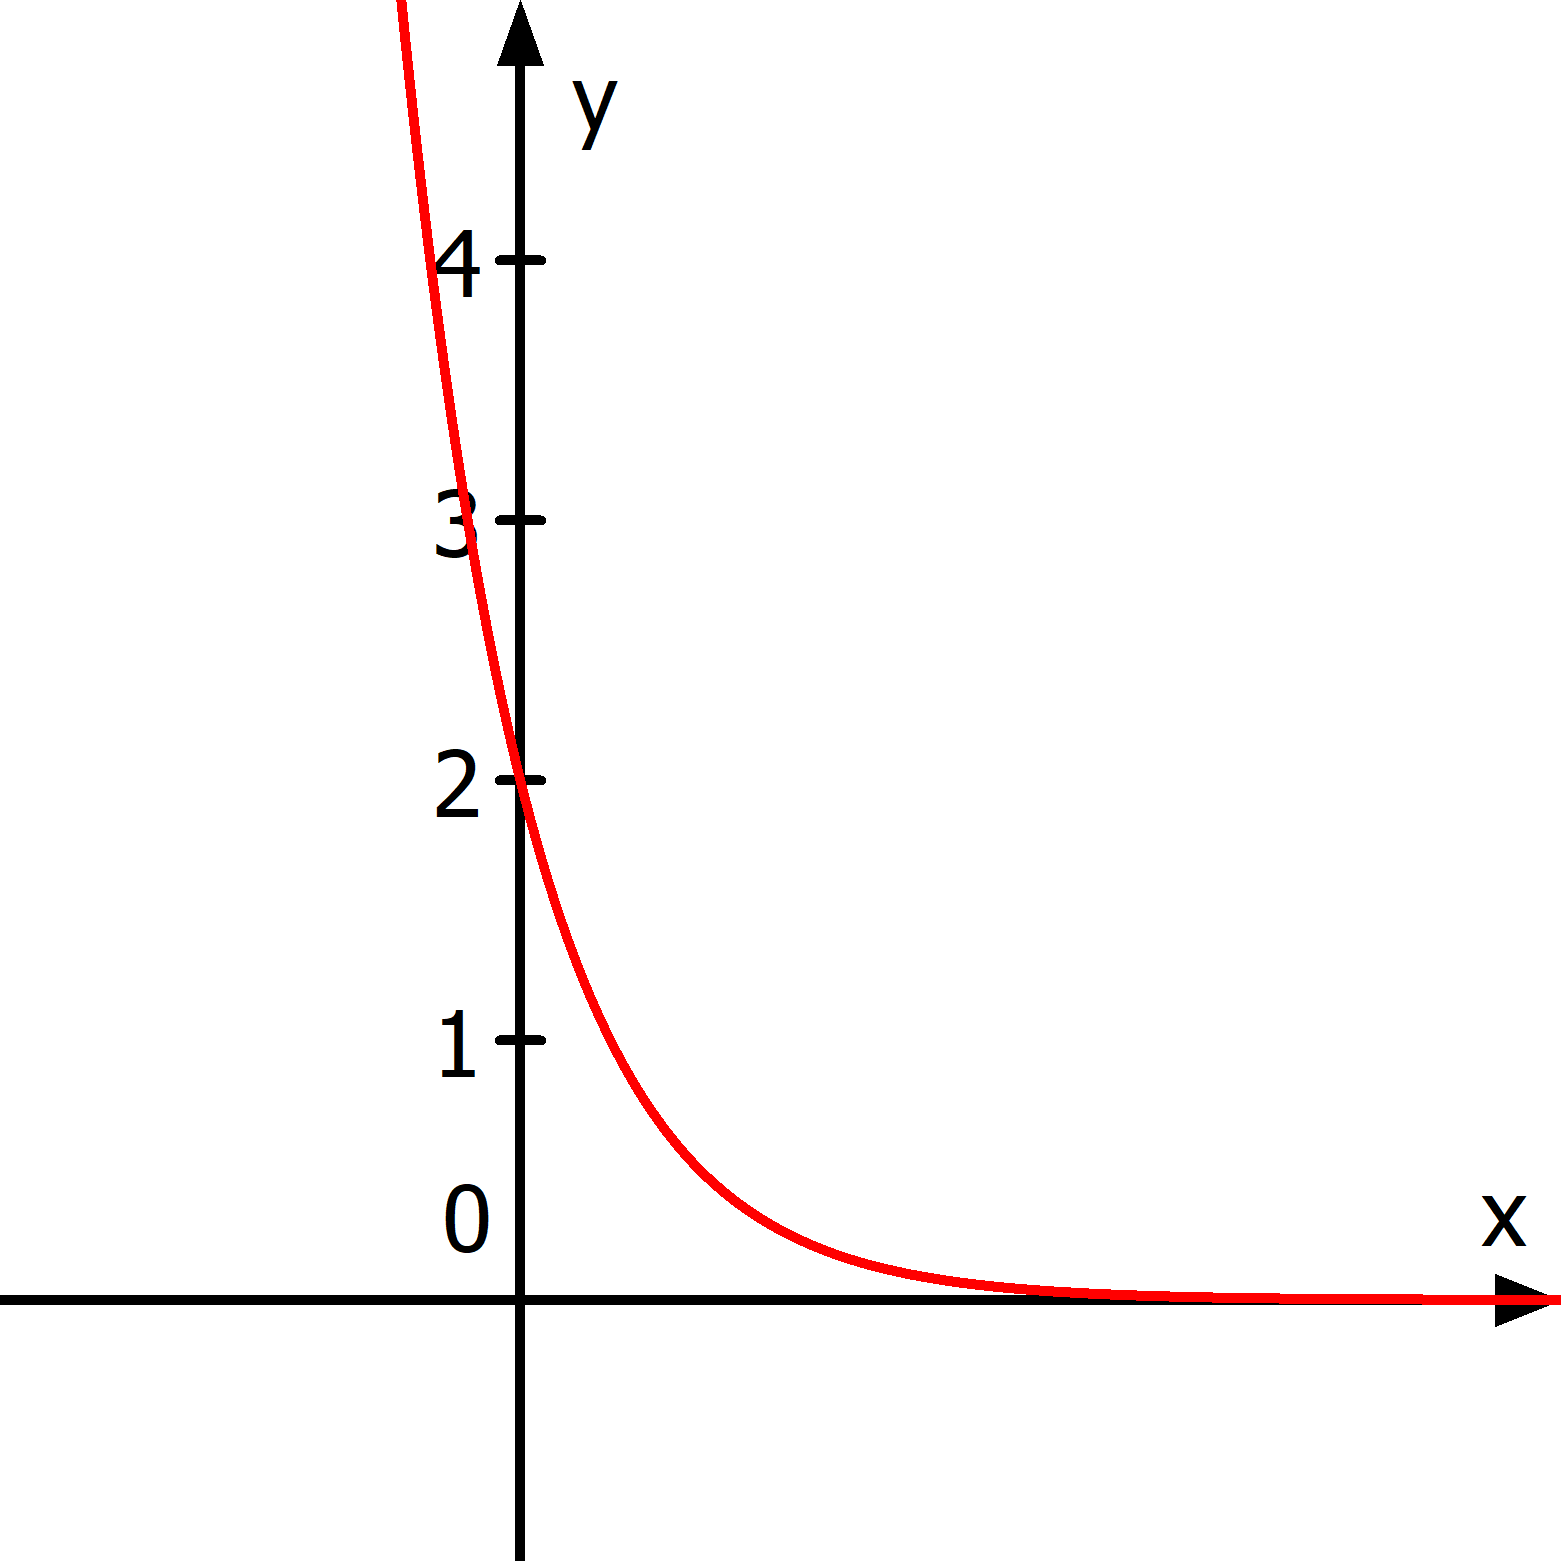
\includegraphics[width=.6\linewidth]{\eFkt/pics/A1k.png}
				\item \(f(x)=-4e^{-7x}\)\\
				Asymptote \(y=0\)\\
				y-Achsenabschnitt: \(f(0)=-4\)\\
				Monoton wachsend\\
				\(f(x)\xrightarrow{\hphantom{\ }x\to-\infty\hphantom{\ }}-\infty\)\\
				\(f(x)\xrightarrow{\hphantom{\ }x\to\infty\hphantom{\ }}0\)\\
				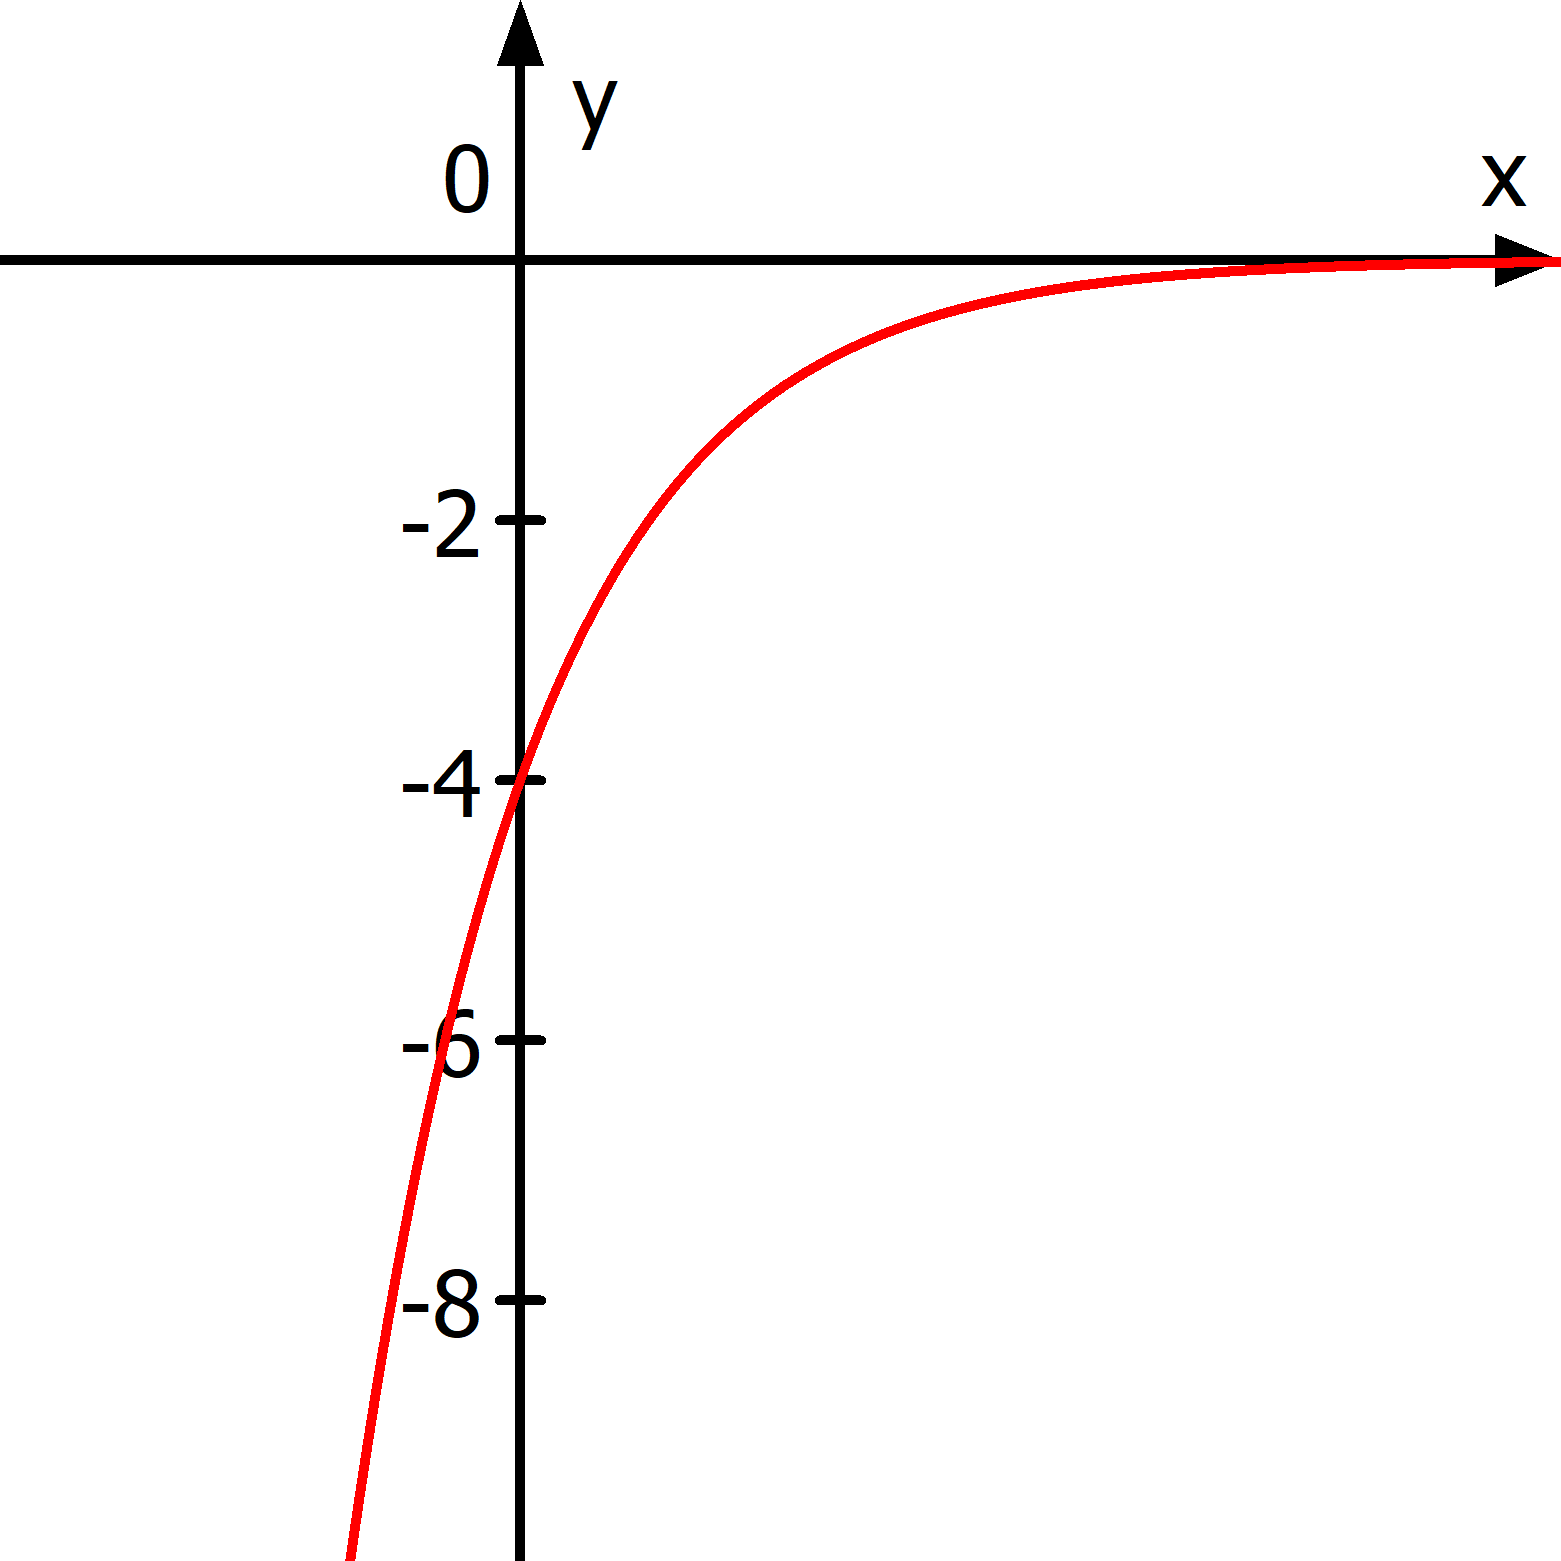
\includegraphics[width=.6\linewidth]{\eFkt/pics/A1l.png}
			\end{enumerate}
		\end{minipage}
	\end{minipage}\\
	%%%%% m bis r
	\begin{minipage}{\textwidth}
		\begin{minipage}[t]{0.49\textwidth}
			\begin{enumerate}[label=\alph*)]
				\setcounter{enumi}{12}
				\item \(f(x)=-\frac{5}{7}e^{x}\)\\
				Asymptote \(y=0\)\\
				y-Achsenabschnitt: \(f(0)=-\frac{5}{7}\)\\
				Monoton fallend\\
				\(f(x)\xrightarrow{\hphantom{\ }x\to-\infty\hphantom{\ }}0\)\\
				\(f(x)\xrightarrow{\hphantom{\ }x\to\infty\hphantom{\ }}-\infty\)\\
				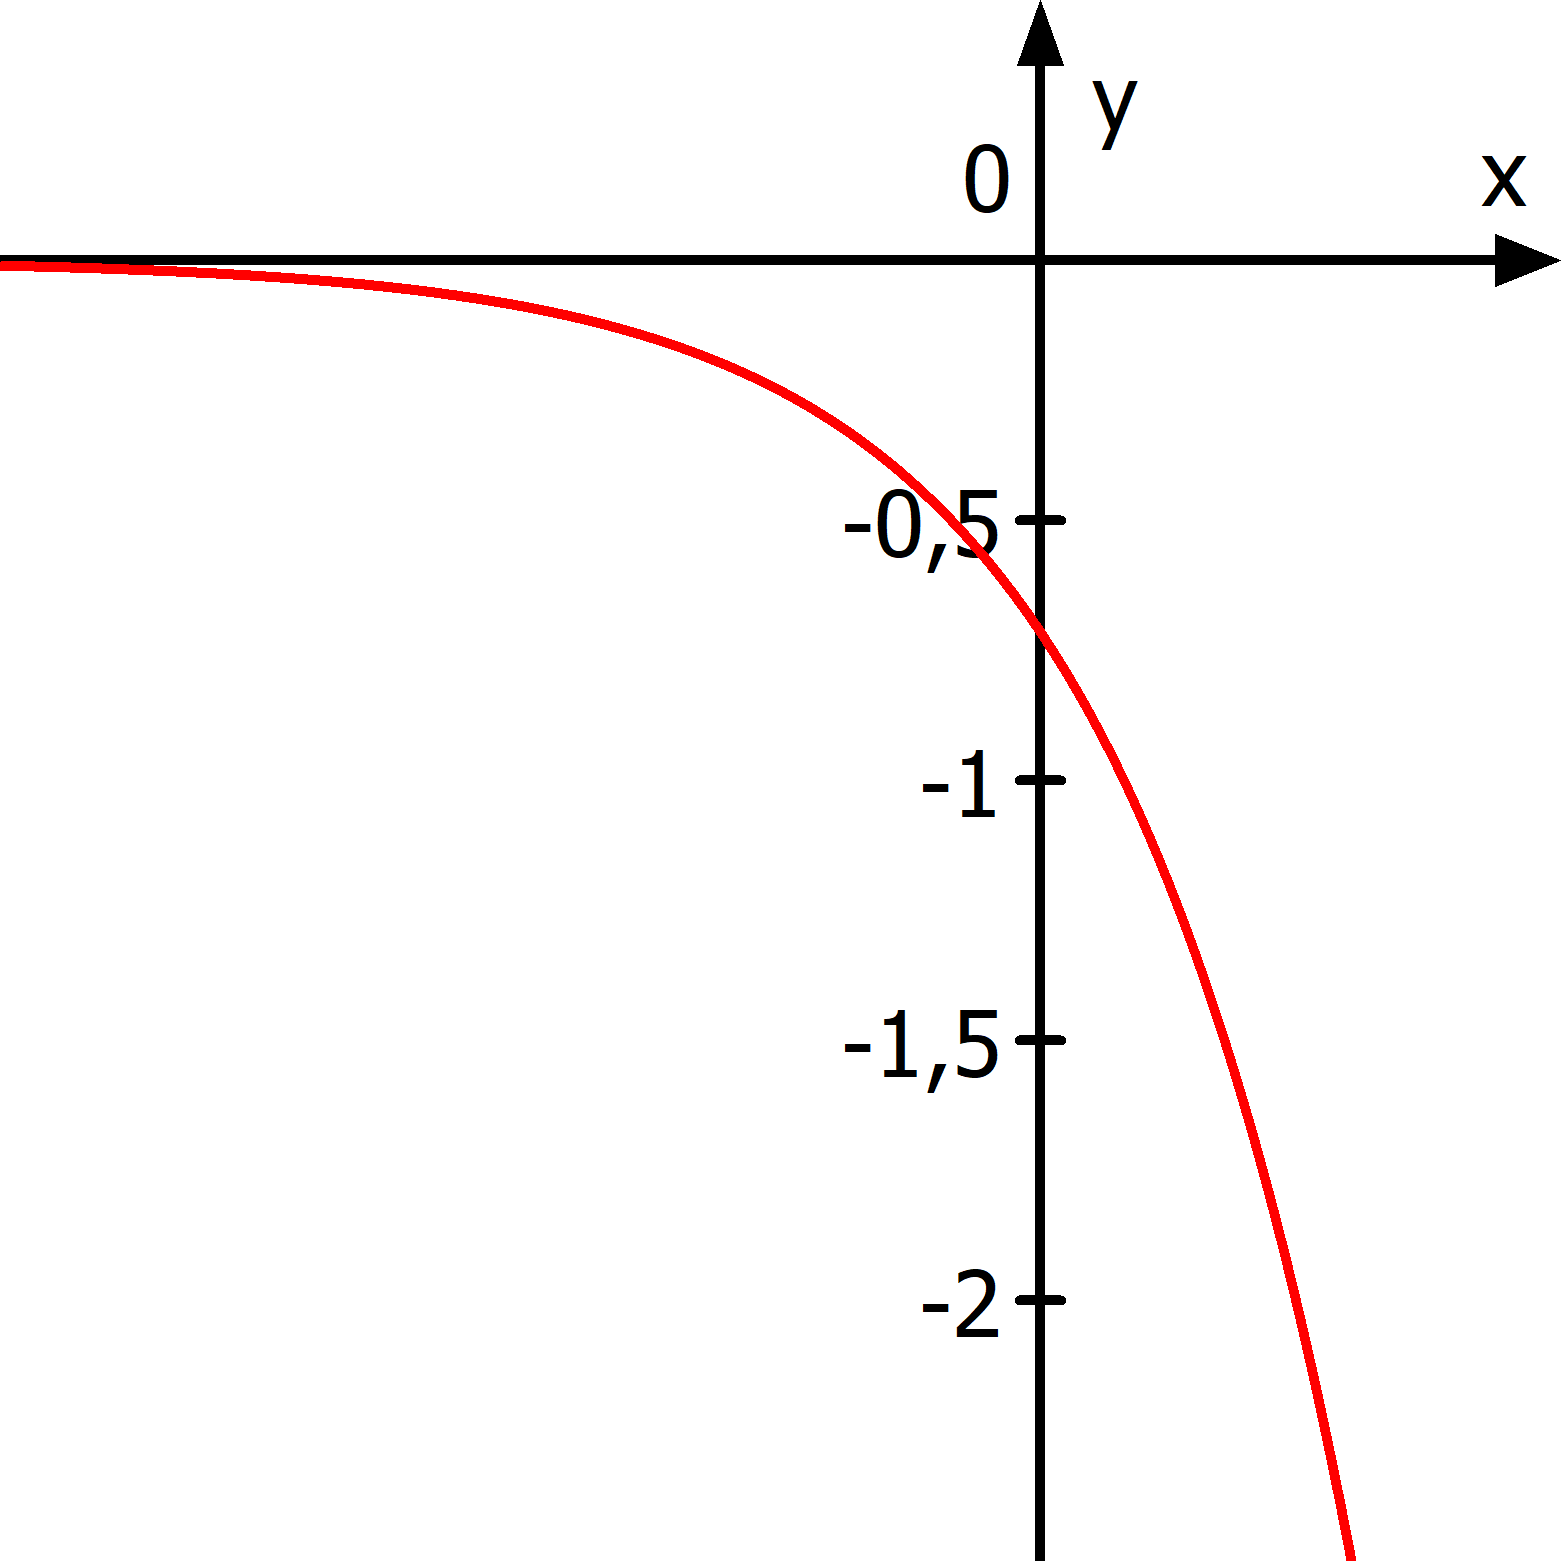
\includegraphics[width=.6\linewidth]{\eFkt/pics/A1m.png}
				\item \(f(x)=6e^{-4x}\)\\
				Asymptote \(y=0\)\\
				y-Achsenabschnitt: \(f(0)=6\)\\
				Monoton fallend\\
				\(f(x)\xrightarrow{\hphantom{\ }x\to-\infty\hphantom{\ }}\infty\)\\
				\(f(x)\xrightarrow{\hphantom{\ }x\to\infty\hphantom{\ }}0\)\\
				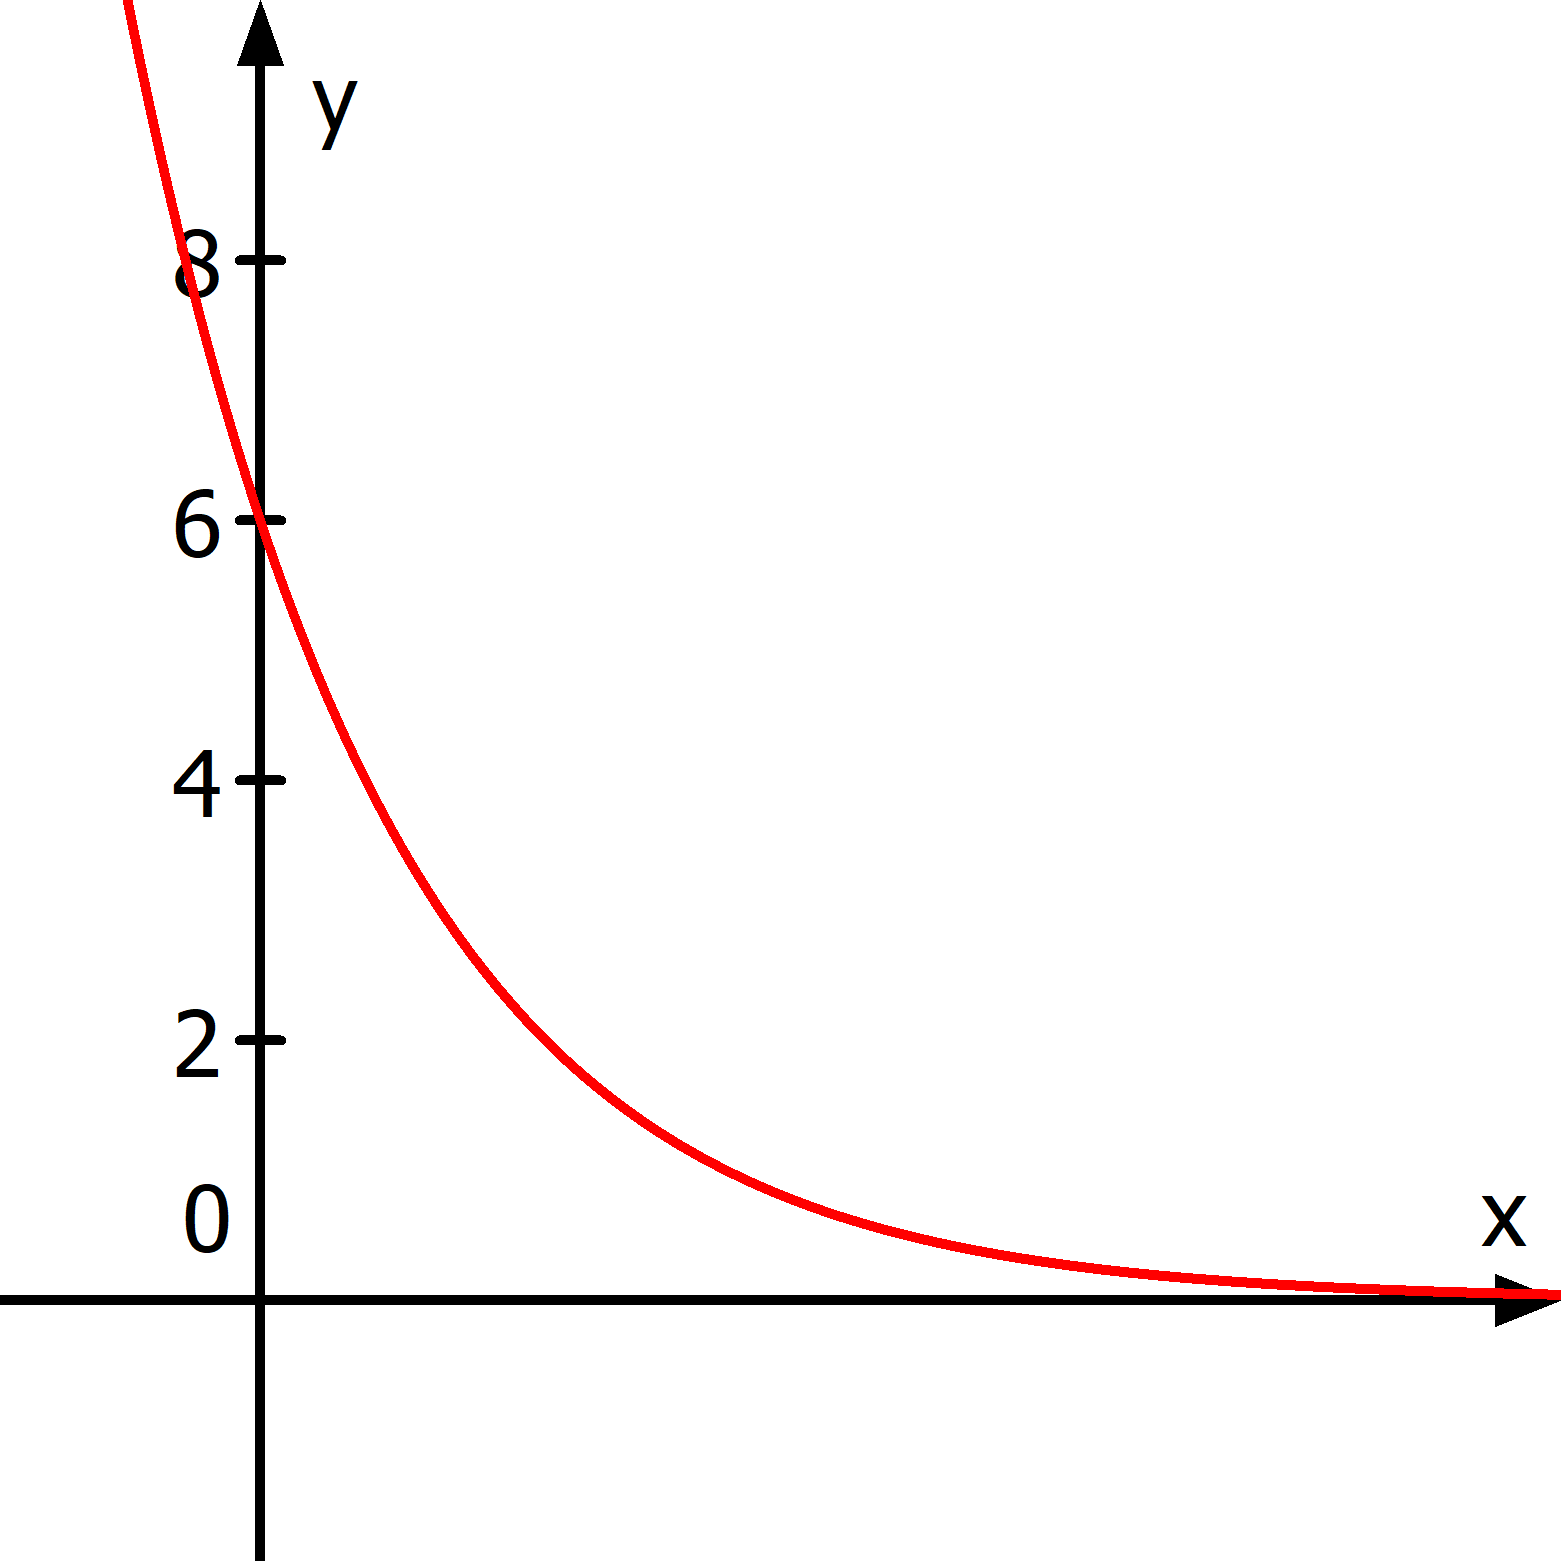
\includegraphics[width=.6\linewidth]{\eFkt/pics/A1n.png}
				\item \(f(x)=-2e^{-8x}\)\\
				Asymptote \(y=0\)\\
				y-Achsenabschnitt: \(f(0)=-2\)\\
				Monoton wachsend\\
				\(f(x)\xrightarrow{\hphantom{\ }x\to-\infty\hphantom{\ }}-\infty\)\\
				\(f(x)\xrightarrow{\hphantom{\ }x\to\infty\hphantom{\ }}0\)\\
				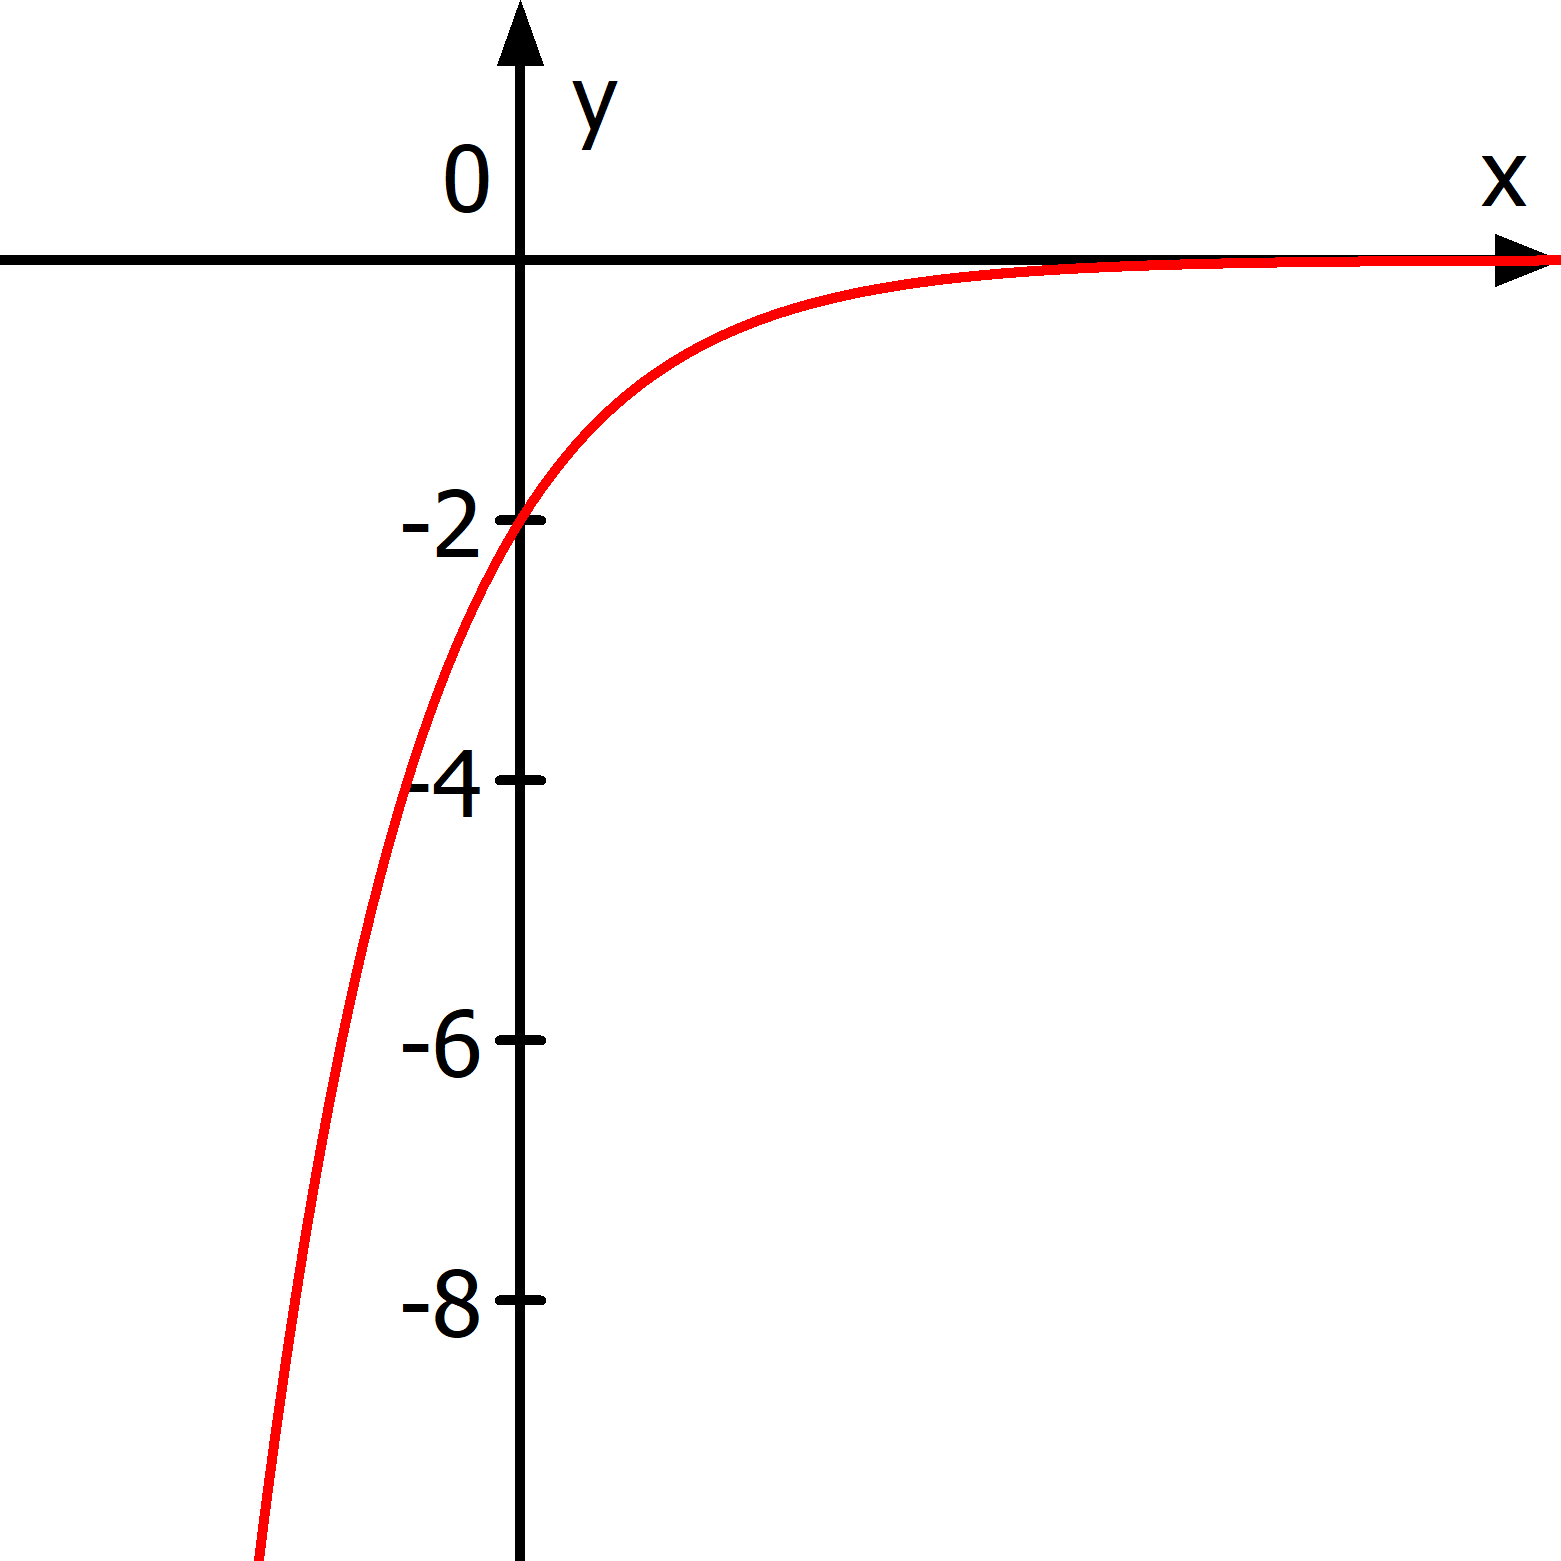
\includegraphics[width=.6\linewidth]{\eFkt/pics/A1o.png}
			\end{enumerate}
		\end{minipage}
		\begin{minipage}[t]{0.49\textwidth}
			\begin{enumerate}[label=\alph*)]
				\setcounter{enumi}{15}
				\item \(f(x)=5,3e^{0,2x}\)\\
				Asymptote \(y=0\)\\
				y-Achsenabschnitt: \(f(0)=5,3\)\\
				Monoton wachsend\\
				\(f(x)\xrightarrow{\hphantom{\ }x\to-\infty\hphantom{\ }}0\)\\
				\(f(x)\xrightarrow{\hphantom{\ }x\to\infty\hphantom{\ }}\infty\)\\
				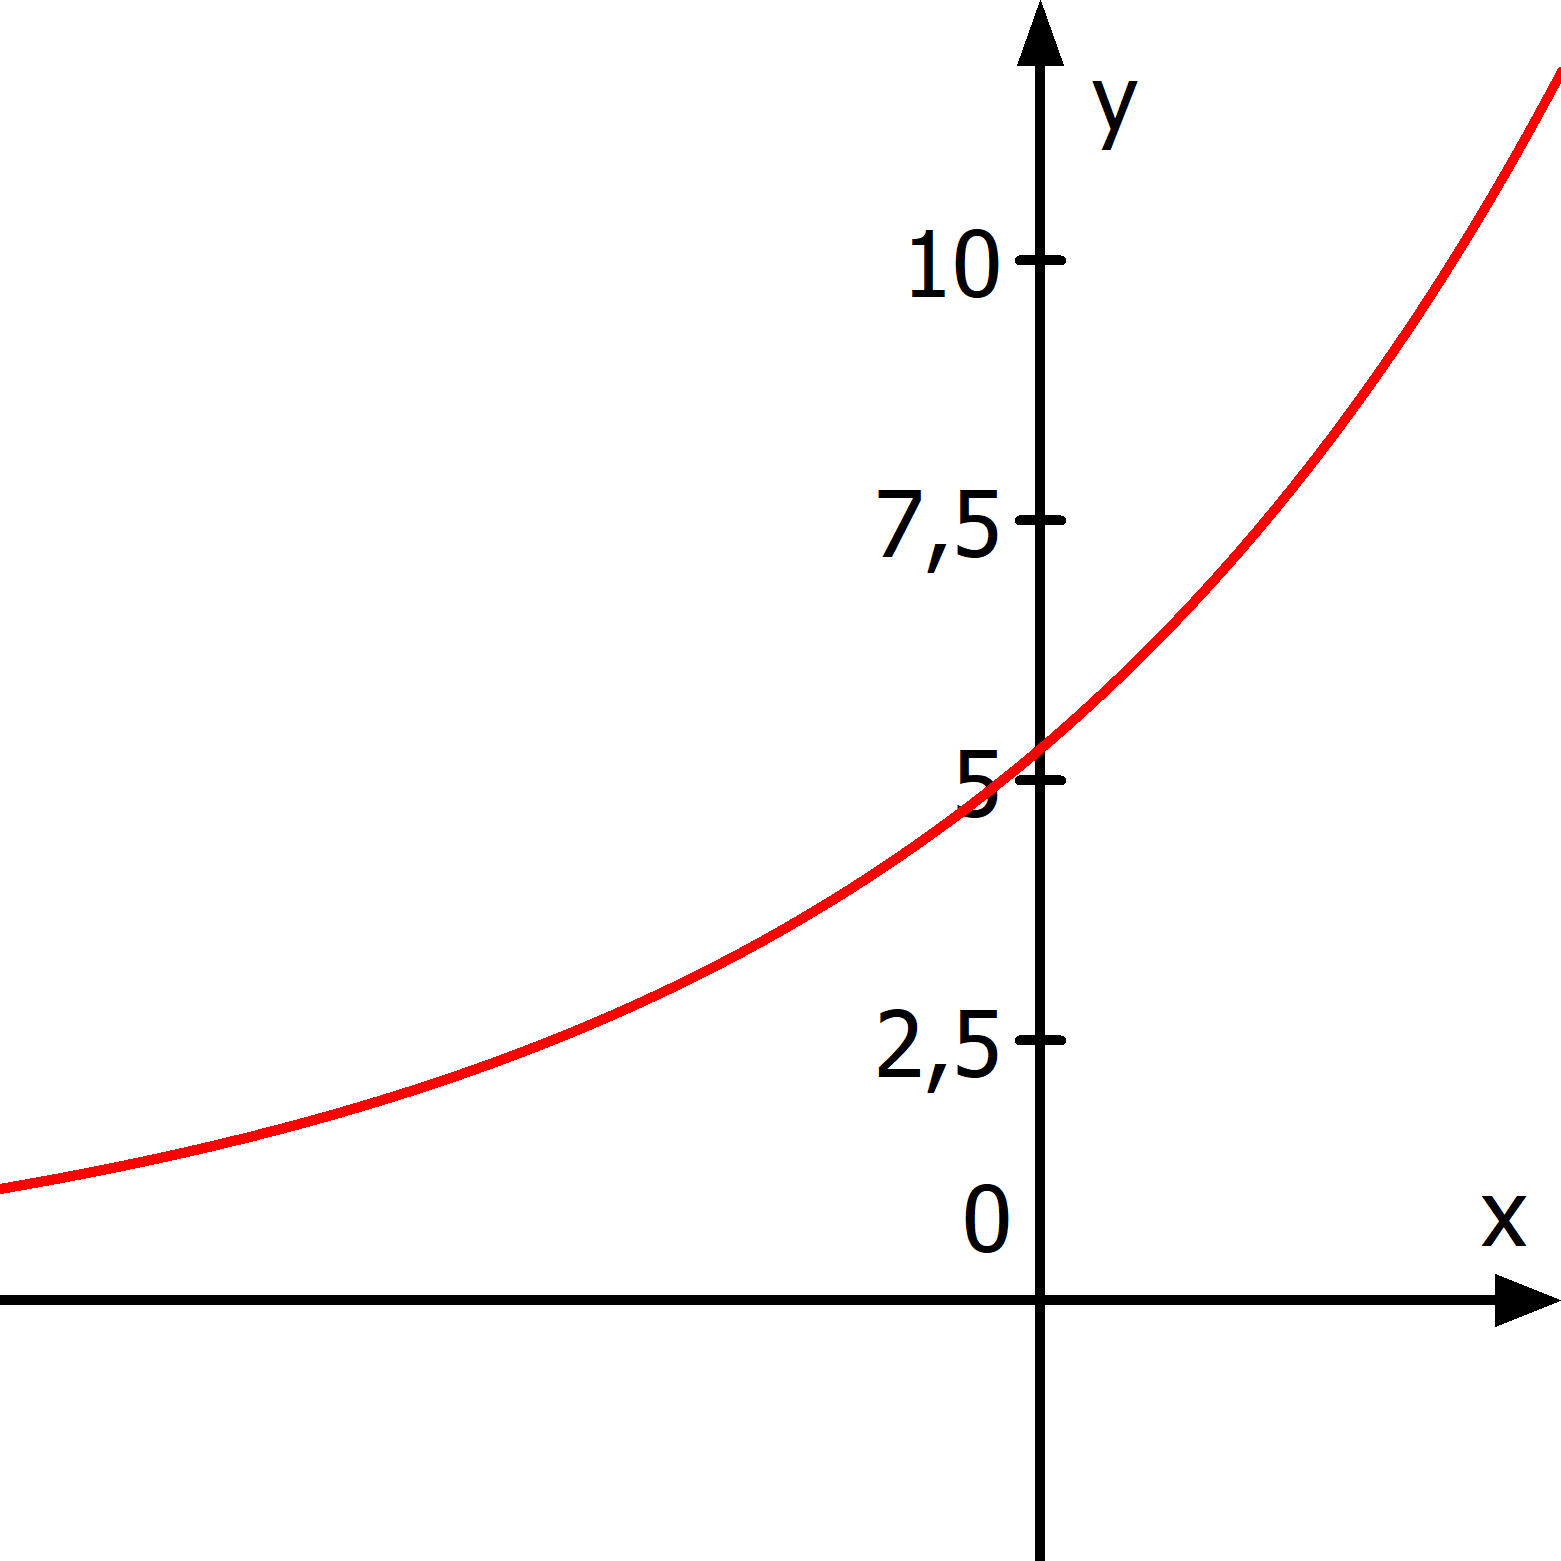
\includegraphics[width=.6\linewidth]{\eFkt/pics/A1p.png}
				\item \(f(x)=-\frac{1}{4}e^{-\frac{2}{3}x}\)\\
				Asymptote \(y=0\)\\
				y-Achsenabschnitt: \(f(0)=-\frac{1}{4}\)\\
				Monoton wachsend\\
				\(f(x)\xrightarrow{\hphantom{\ }x\to-\infty\hphantom{\ }}-\infty\)\\
				\(f(x)\xrightarrow{\hphantom{\ }x\to\infty\hphantom{\ }}0\)\\
				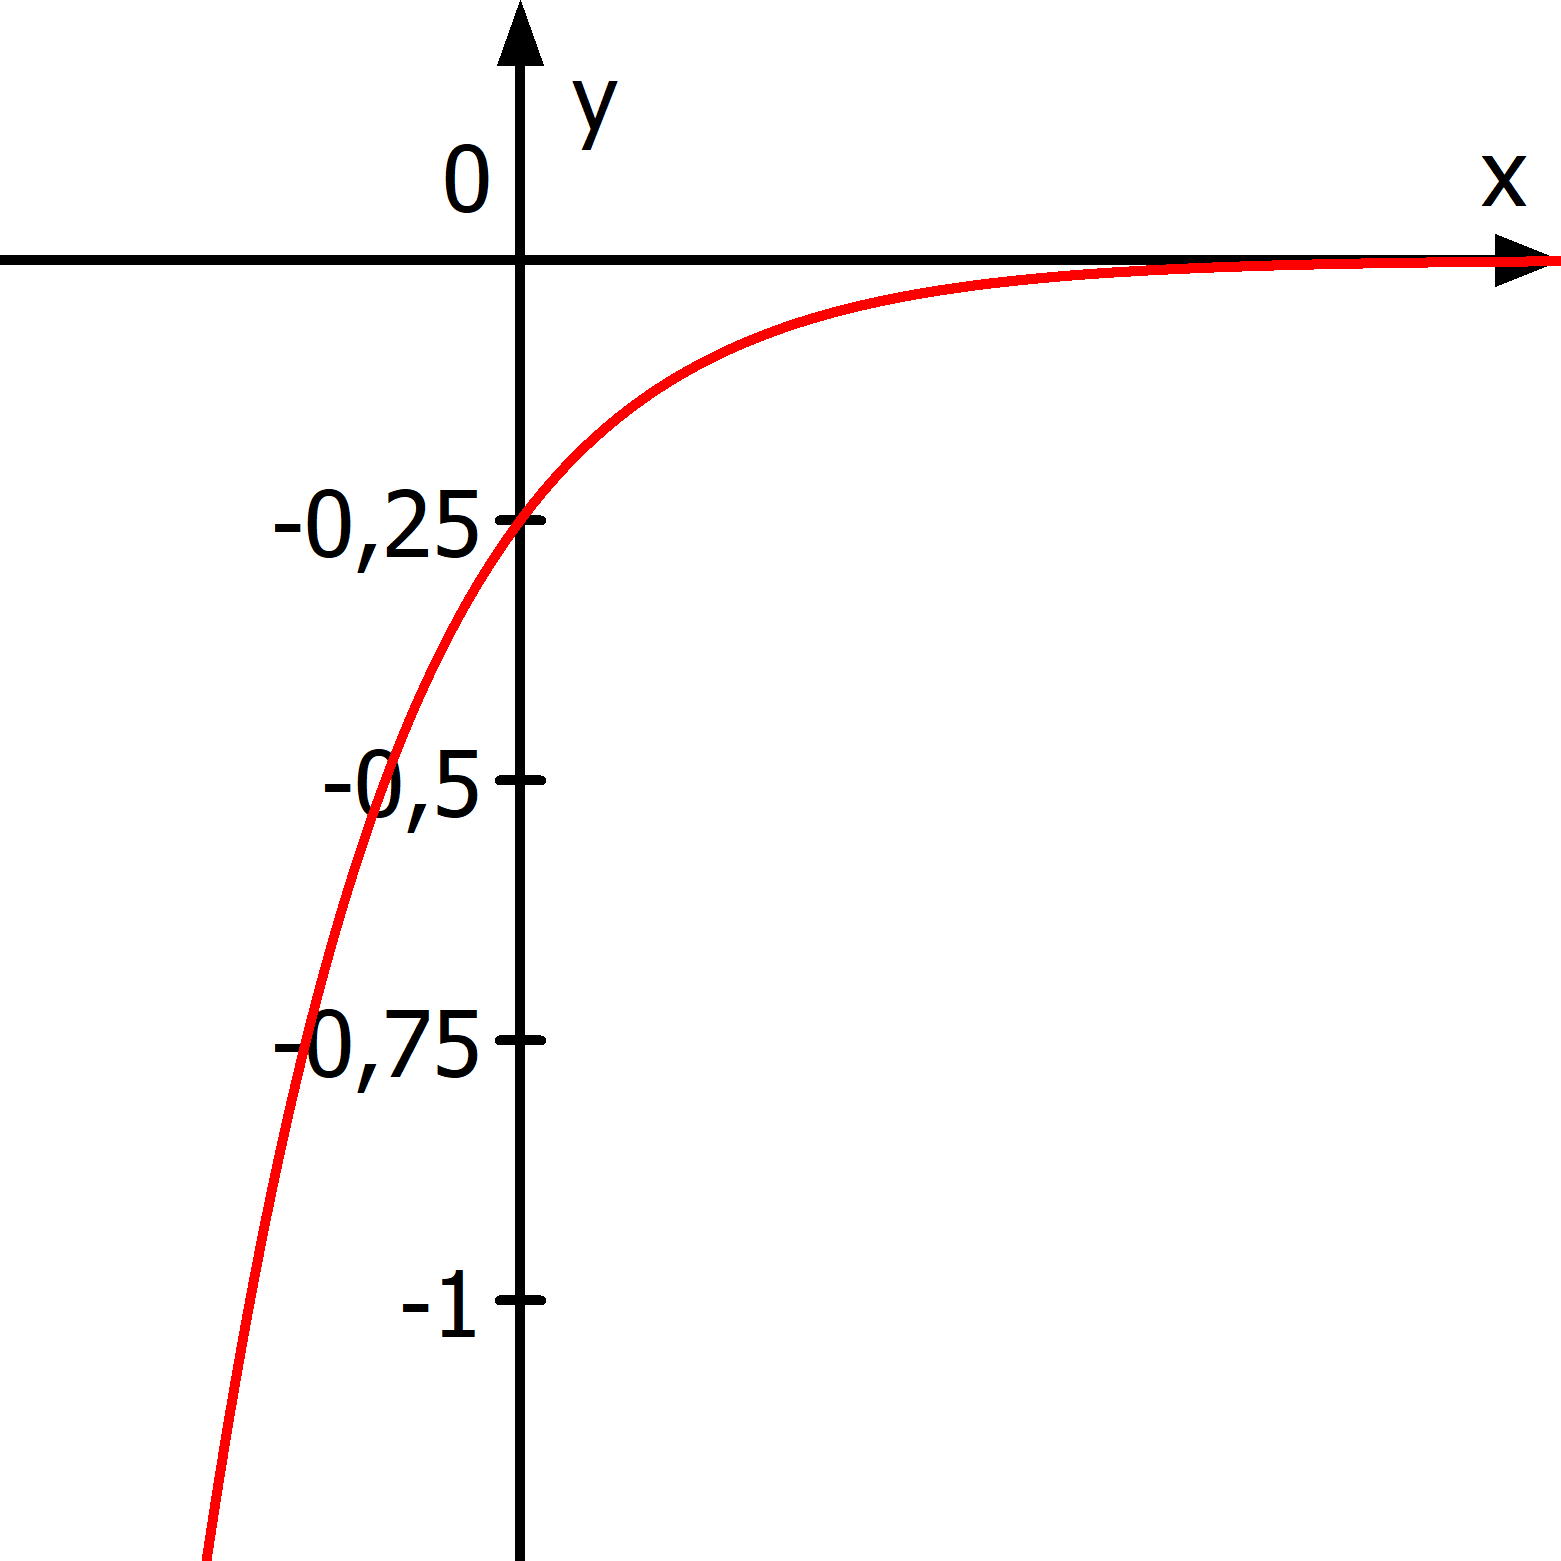
\includegraphics[width=.6\linewidth]{\eFkt/pics/A1q.png}
				\item \(f(x)=-2e^{0,2x}\)\\
				Asymptote \(y=0\)\\
				y-Achsenabschnitt: \(f(0)=-2\)\\
				Monoton fallend\\
				\(f(x)\xrightarrow{\hphantom{\ }x\to-\infty\hphantom{\ }}0\)\\
				\(f(x)\xrightarrow{\hphantom{\ }x\to\infty\hphantom{\ }}-\infty\)\\
				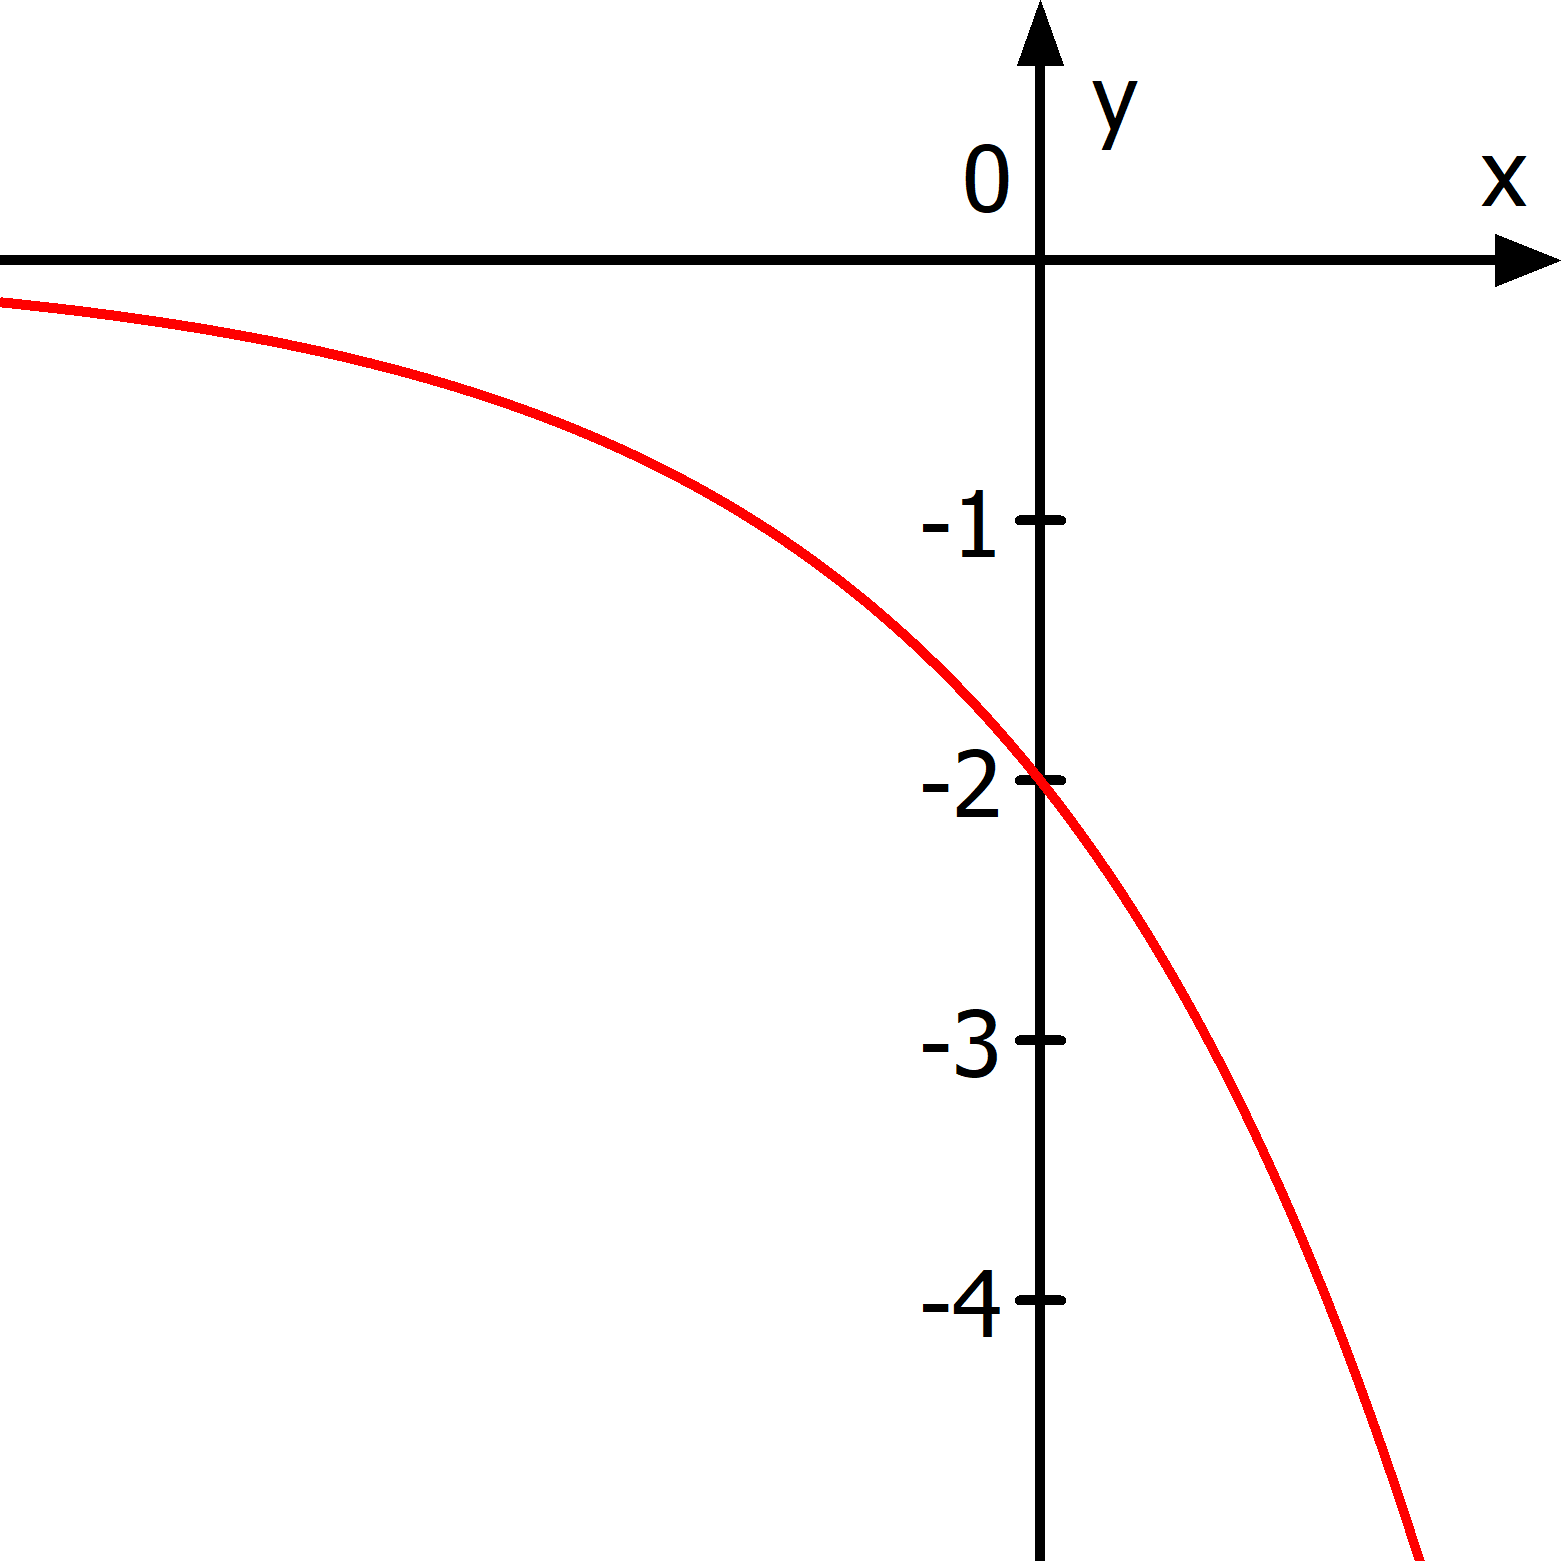
\includegraphics[width=.6\linewidth]{\eFkt/pics/A1r.png}
			\end{enumerate}
		\end{minipage}
	\end{minipage}\\
	%%%%% s bis x
	\begin{minipage}{\textwidth}
		\begin{minipage}[t]{0.49\textwidth}
			\begin{enumerate}[label=\alph*)]
				\setcounter{enumi}{18}
				\item \(f(x)=1,8e^{-4x}\)\\
				Asymptote \(y=0\)\\
				y-Achsenabschnitt: \(f(0)=1,8\)\\
				Monoton fallend\\
				\(f(x)\xrightarrow{\hphantom{\ }x\to-\infty\hphantom{\ }}\infty\)\\
				\(f(x)\xrightarrow{\hphantom{\ }x\to\infty\hphantom{\ }}0\)\\
				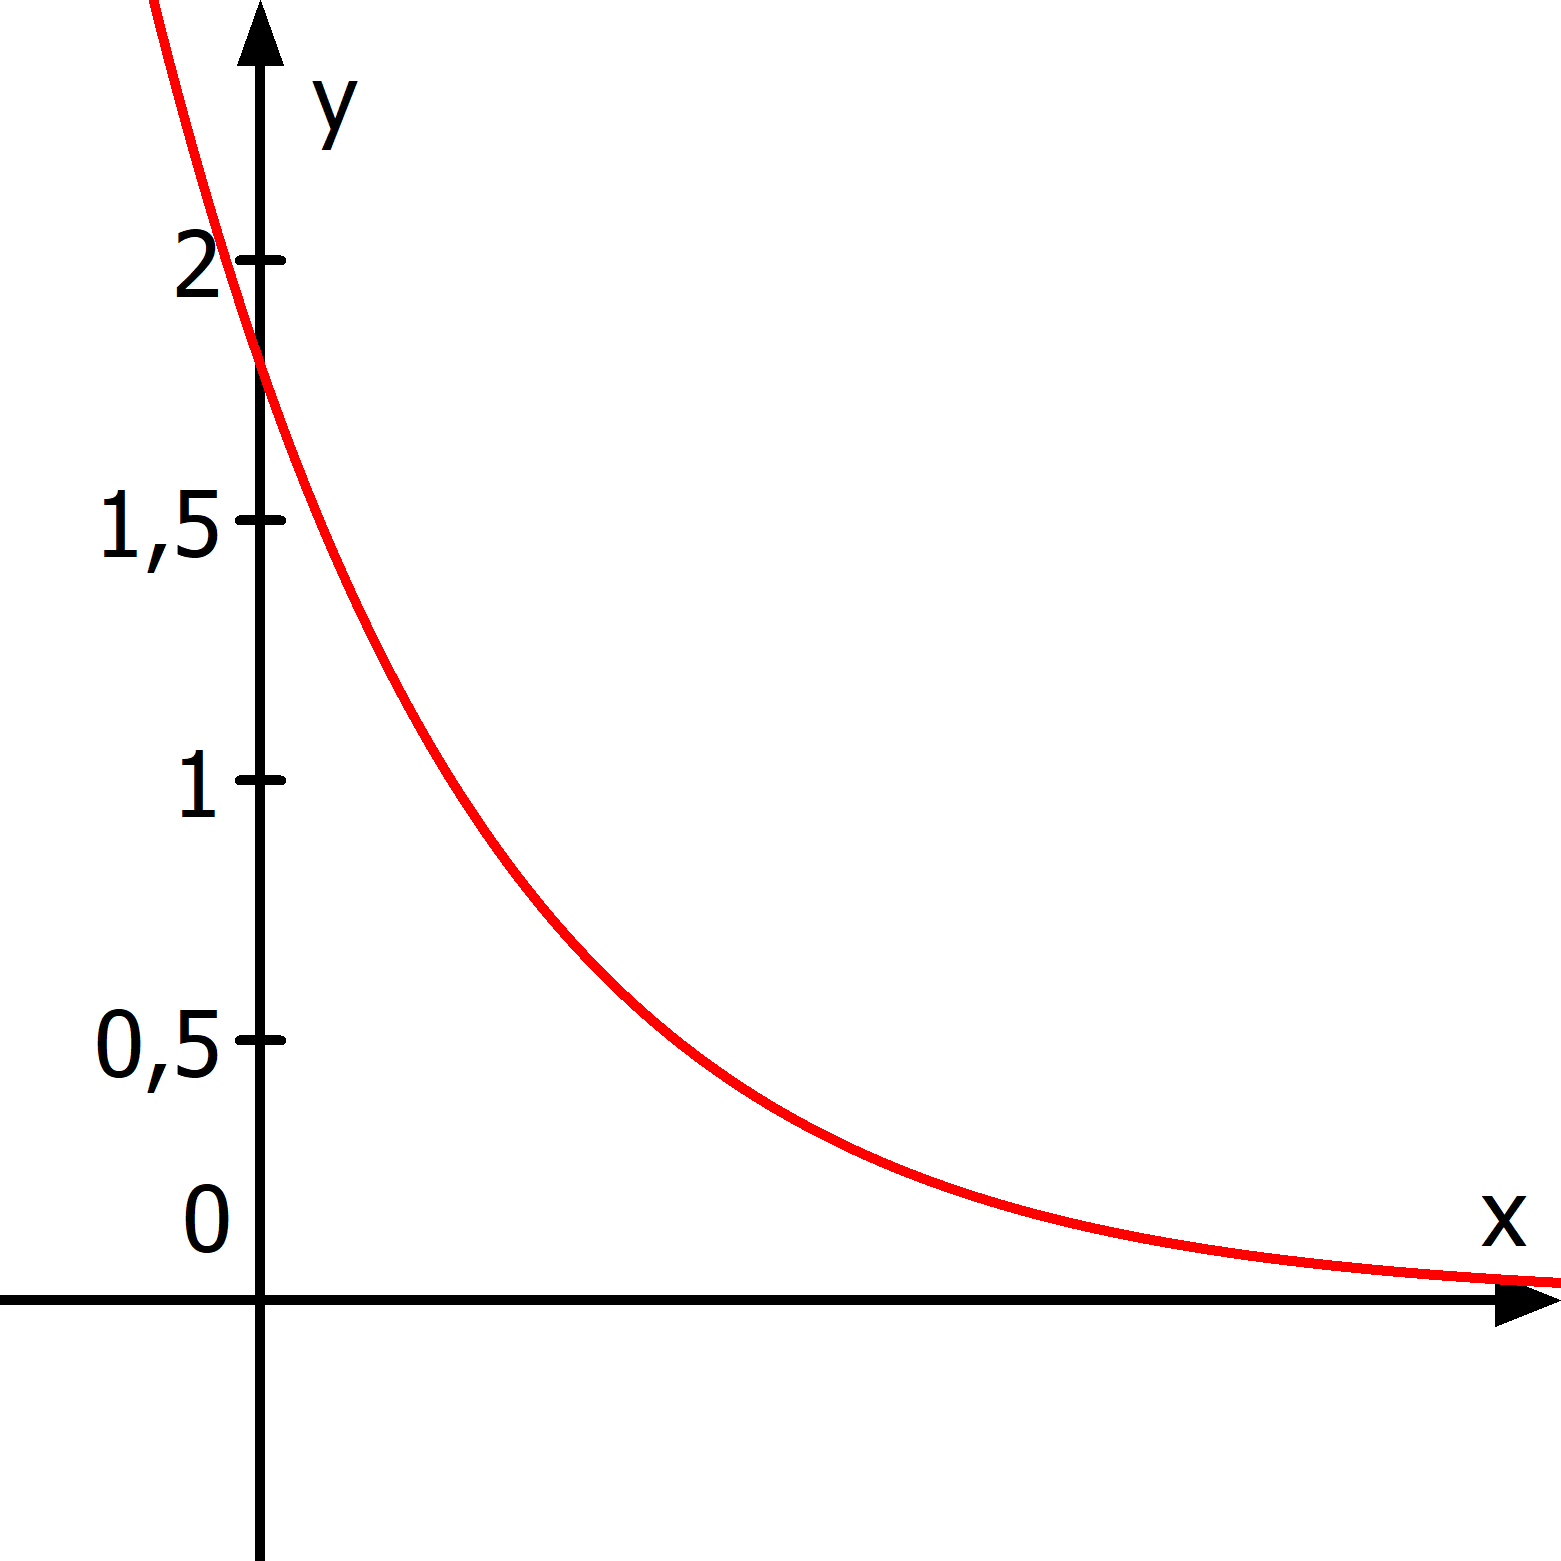
\includegraphics[width=.6\linewidth]{\eFkt/pics/A1s.png}
				\item \(f(x)=5e^{7x}\)\\
				Asymptote \(y=0\)\\
				y-Achsenabschnitt: \(f(0)=5\)\\
				Monoton wachsend\\
				\(f(x)\xrightarrow{\hphantom{\ }x\to-\infty\hphantom{\ }}0\)\\
				\(f(x)\xrightarrow{\hphantom{\ }x\to\infty\hphantom{\ }}\infty\)\\
				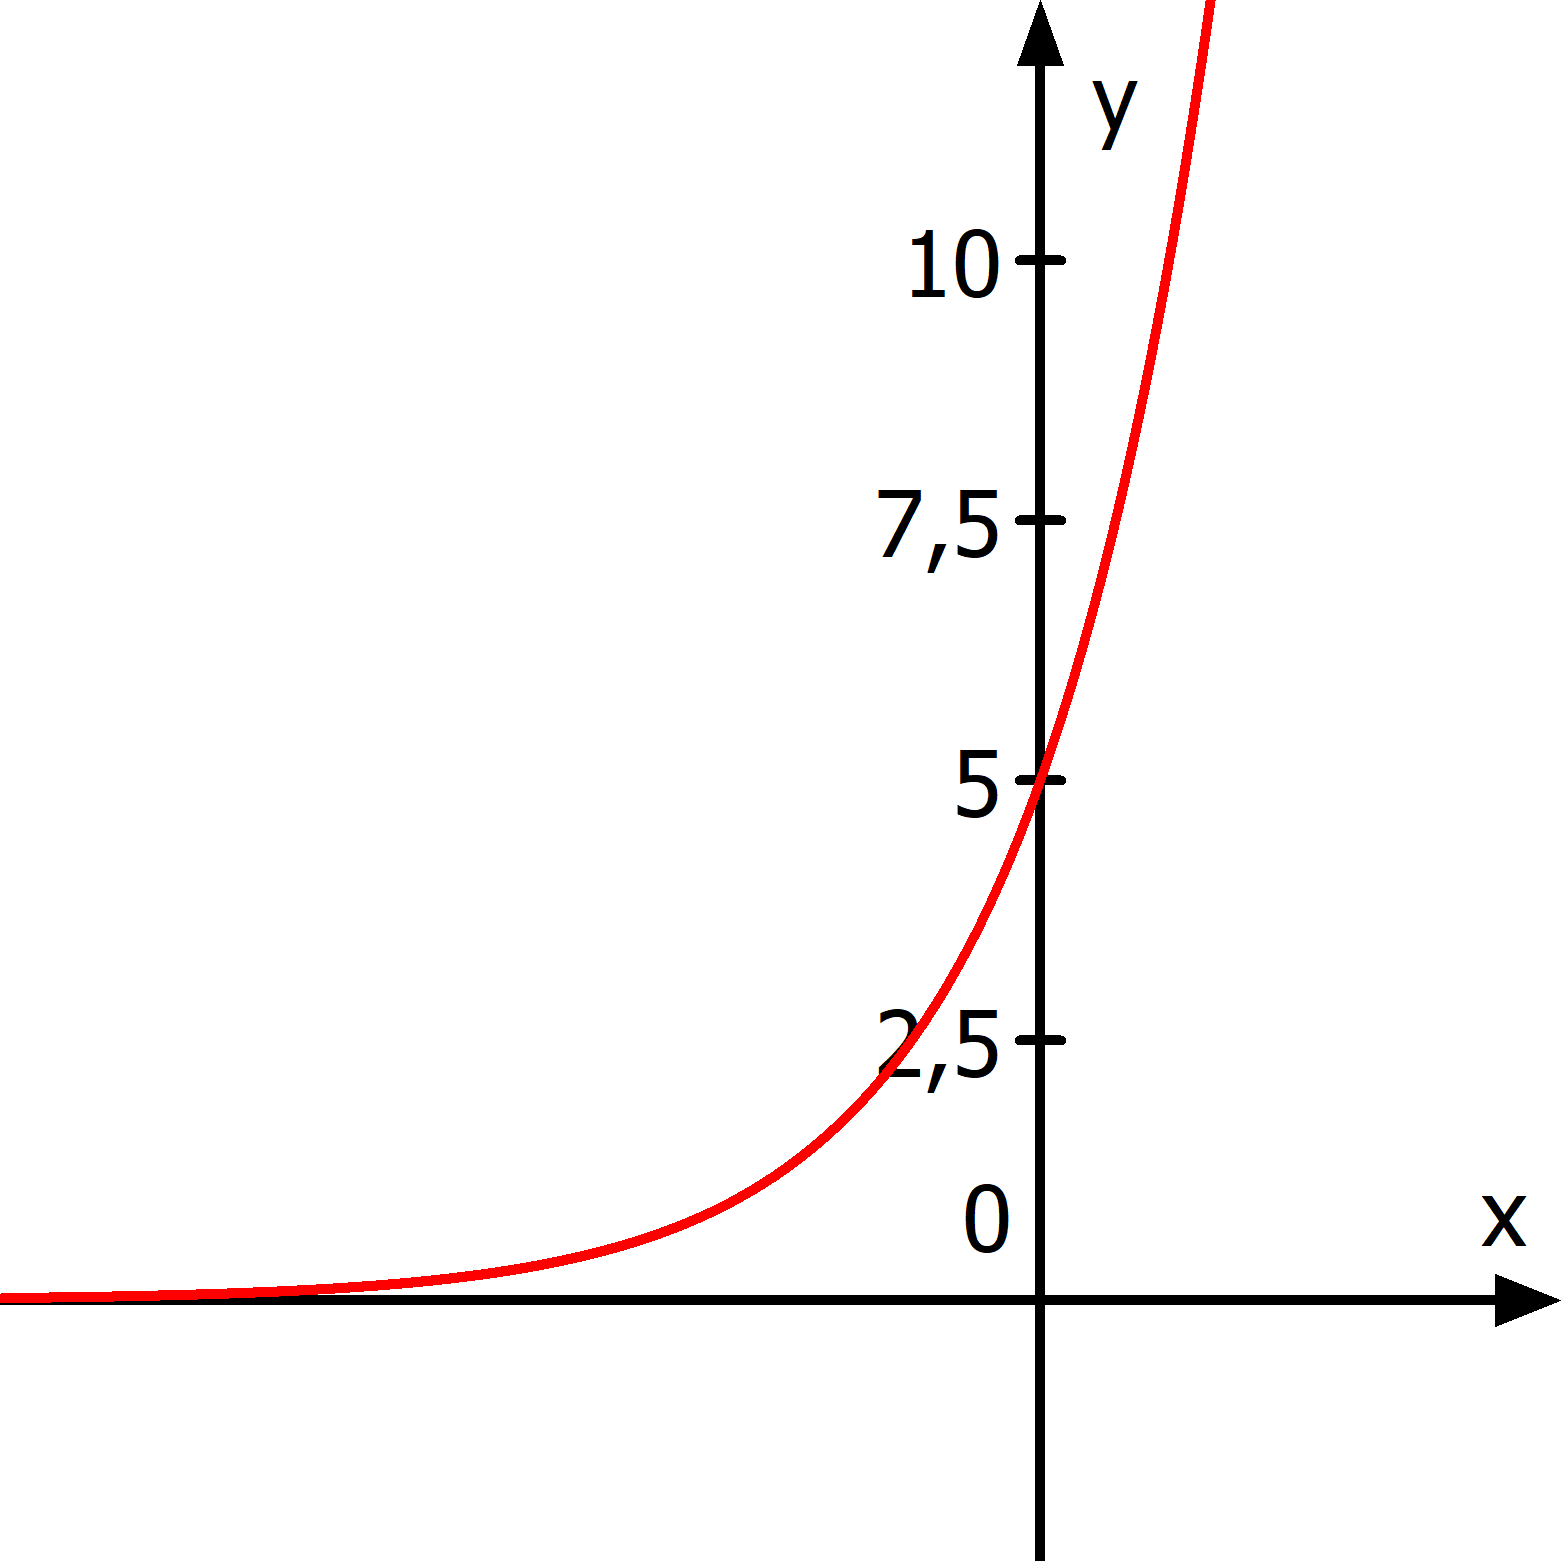
\includegraphics[width=.6\linewidth]{\eFkt/pics/A1t.png}
				\item \(f(x)=-\frac{8}{3}e^{\frac{3}{8}x}\)\\
				Asymptote \(y=0\)\\
				y-Achsenabschnitt: \(f(0)=-\frac{8}{3}\)\\
				Monoton fallend\\
				\(f(x)\xrightarrow{\hphantom{\ }x\to-\infty\hphantom{\ }}0\)\\
				\(f(x)\xrightarrow{\hphantom{\ }x\to\infty\hphantom{\ }}-\infty\)\\
				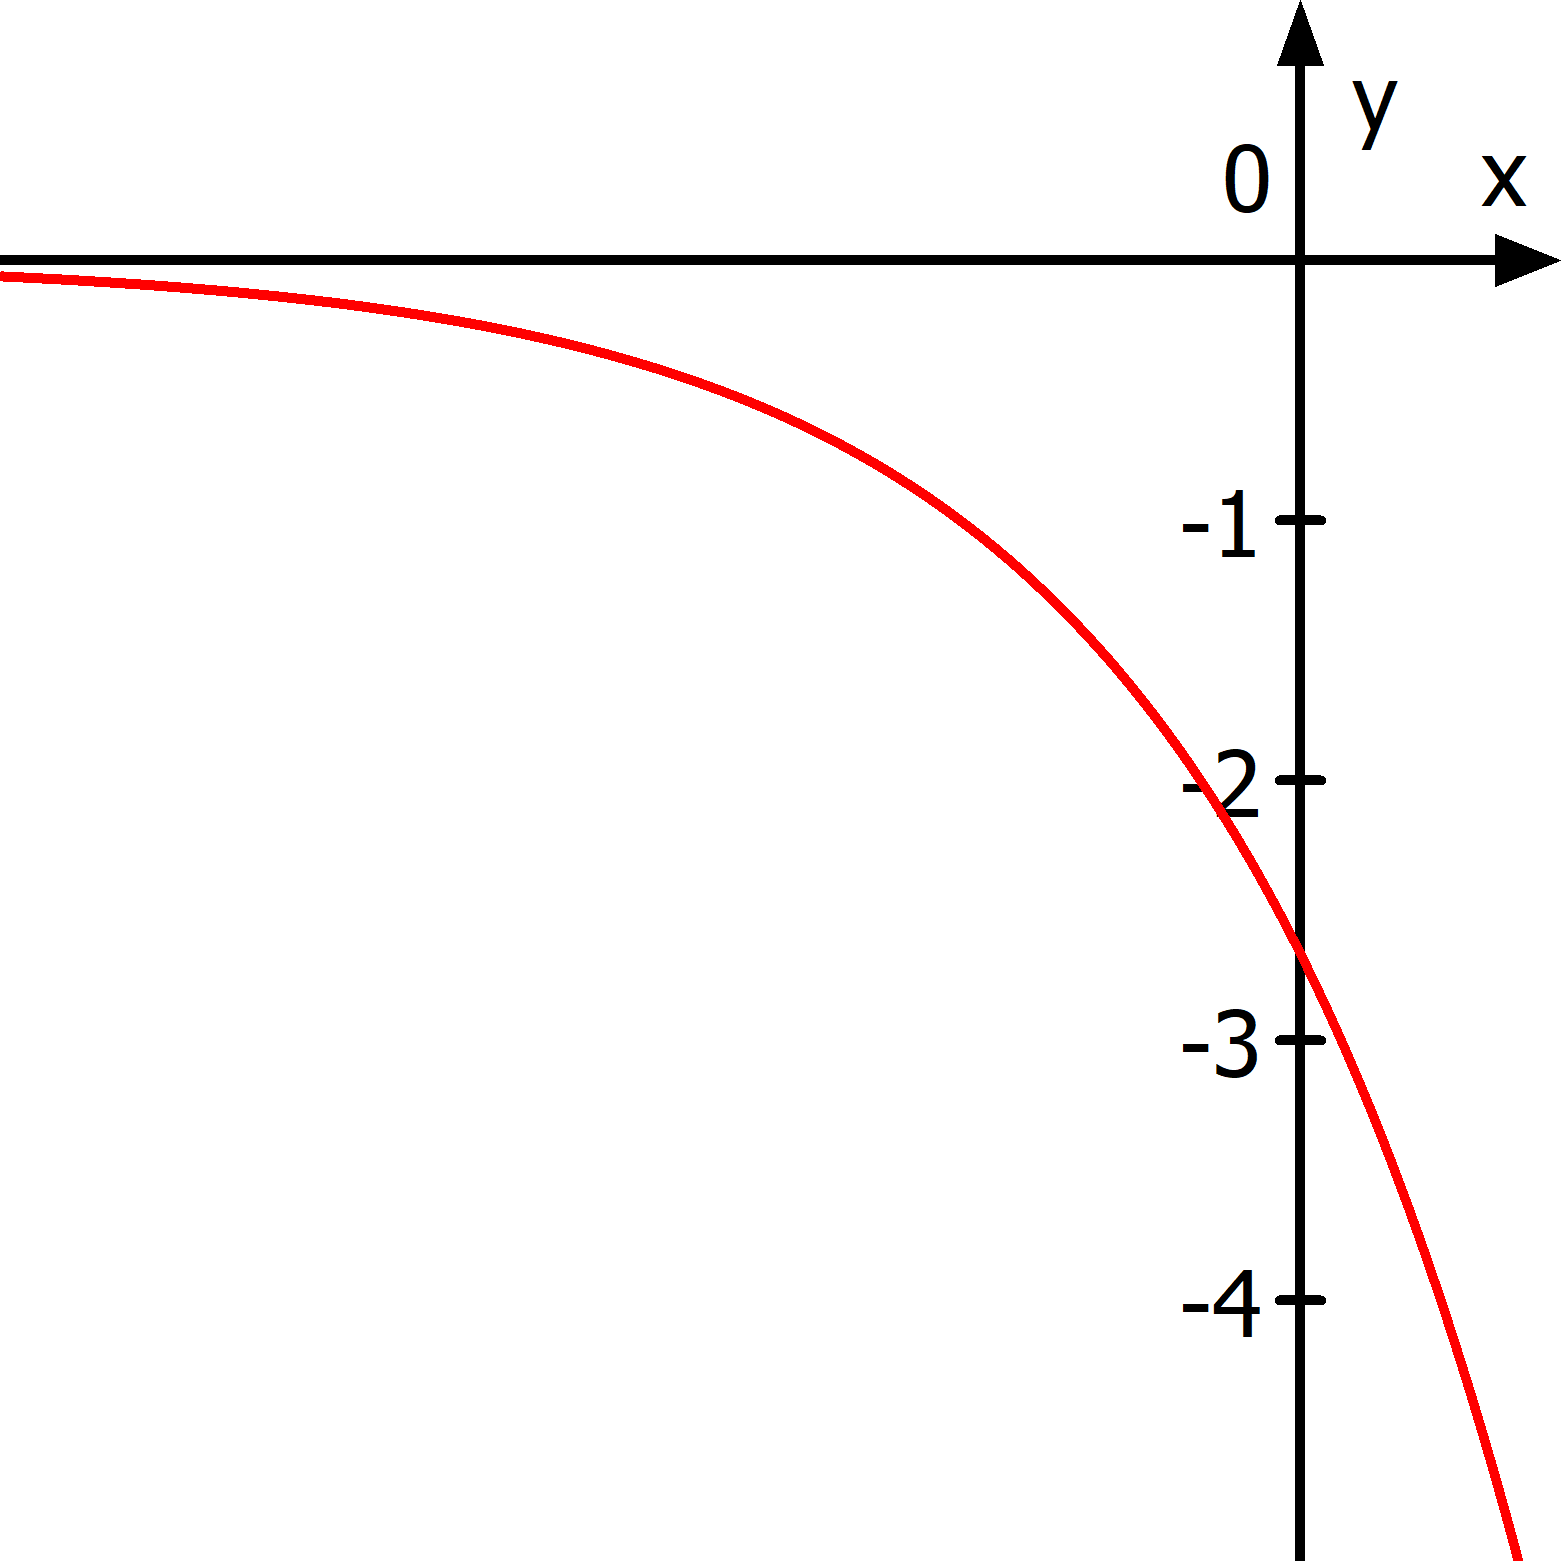
\includegraphics[width=.6\linewidth]{\eFkt/pics/A1u.png}
			\end{enumerate}
		\end{minipage}
		\begin{minipage}[t]{0.49\textwidth}
			\begin{enumerate}[label=\alph*)]
				\setcounter{enumi}{21}
				\item \(f(x)=-0,1^{-0,3x}\)\\
				Asymptote \(y=0\)\\
				y-Achsenabschnitt: \(f(0)=-0,1\)\\
				Monoton wachsend\\
				\(f(x)\xrightarrow{\hphantom{\ }x\to-\infty\hphantom{\ }}-\infty\)\\
				\(f(x)\xrightarrow{\hphantom{\ }x\to\infty\hphantom{\ }}0\)\\
				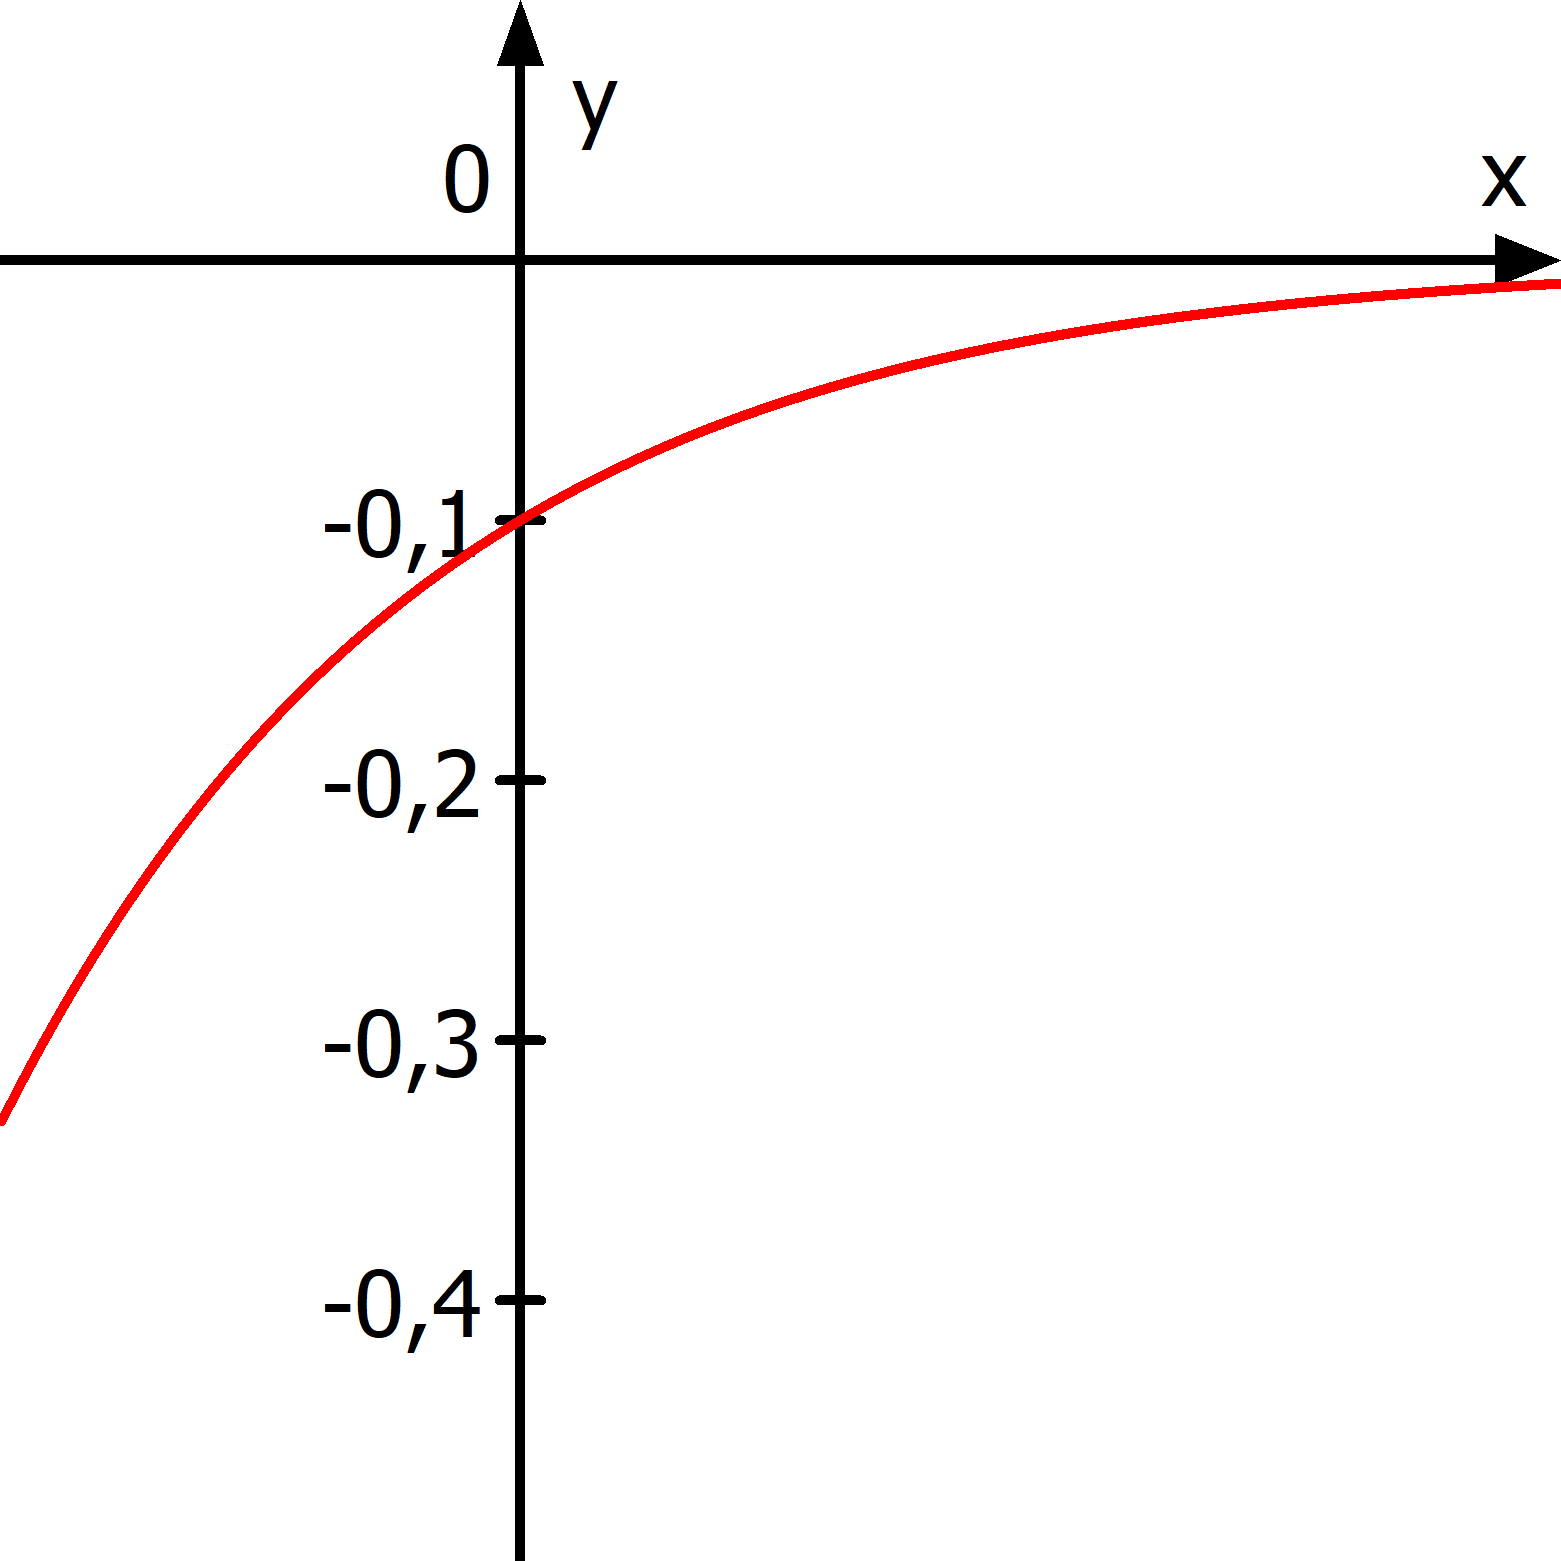
\includegraphics[width=.6\linewidth]{\eFkt/pics/A1v.png}
				\item \(f(x)=10e^{-4x}\)\\
				Asymptote \(y=0\)\\
				y-Achsenabschnitt: \(f(0)=10\)\\
				Monoton fallend\\
				\(f(x)\xrightarrow{\hphantom{\ }x\to-\infty\hphantom{\ }}\infty\)\\
				\(f(x)\xrightarrow{\hphantom{\ }x\to\infty\hphantom{\ }}0\)\\
				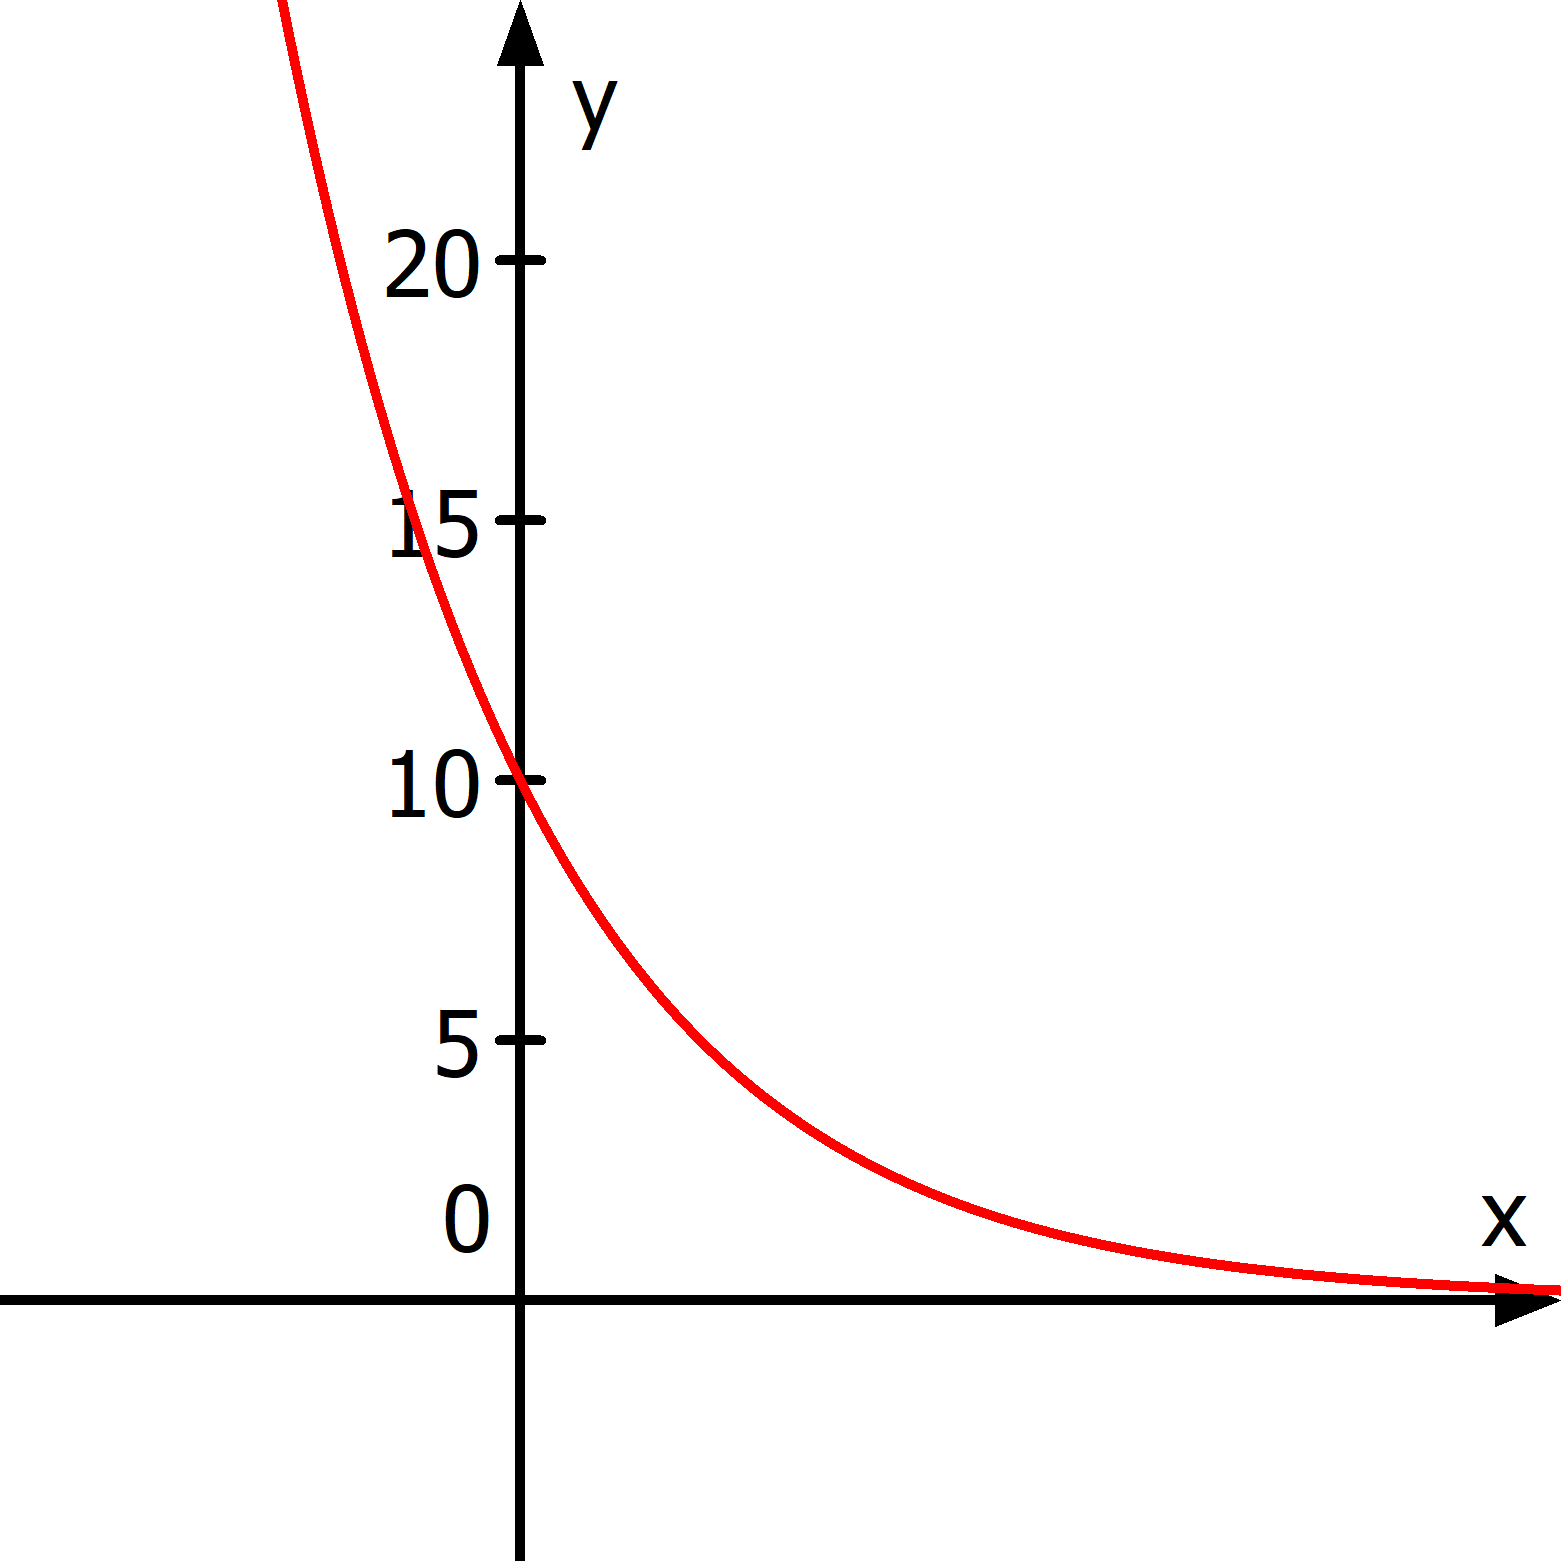
\includegraphics[width=.6\linewidth]{\eFkt/pics/A1w.png}
				\item \(f(x)=-5e^{6x}\)\\
				Asymptote \(y=0\)\\
				y-Achsenabschnitt: \(f(0)=-5\)\\
				Monoton fallend\\
				\(f(x)\xrightarrow{\hphantom{\ }x\to-\infty\hphantom{\ }}0\)\\
				\(f(x)\xrightarrow{\hphantom{\ }x\to\infty\hphantom{\ }}-\infty\)\\
				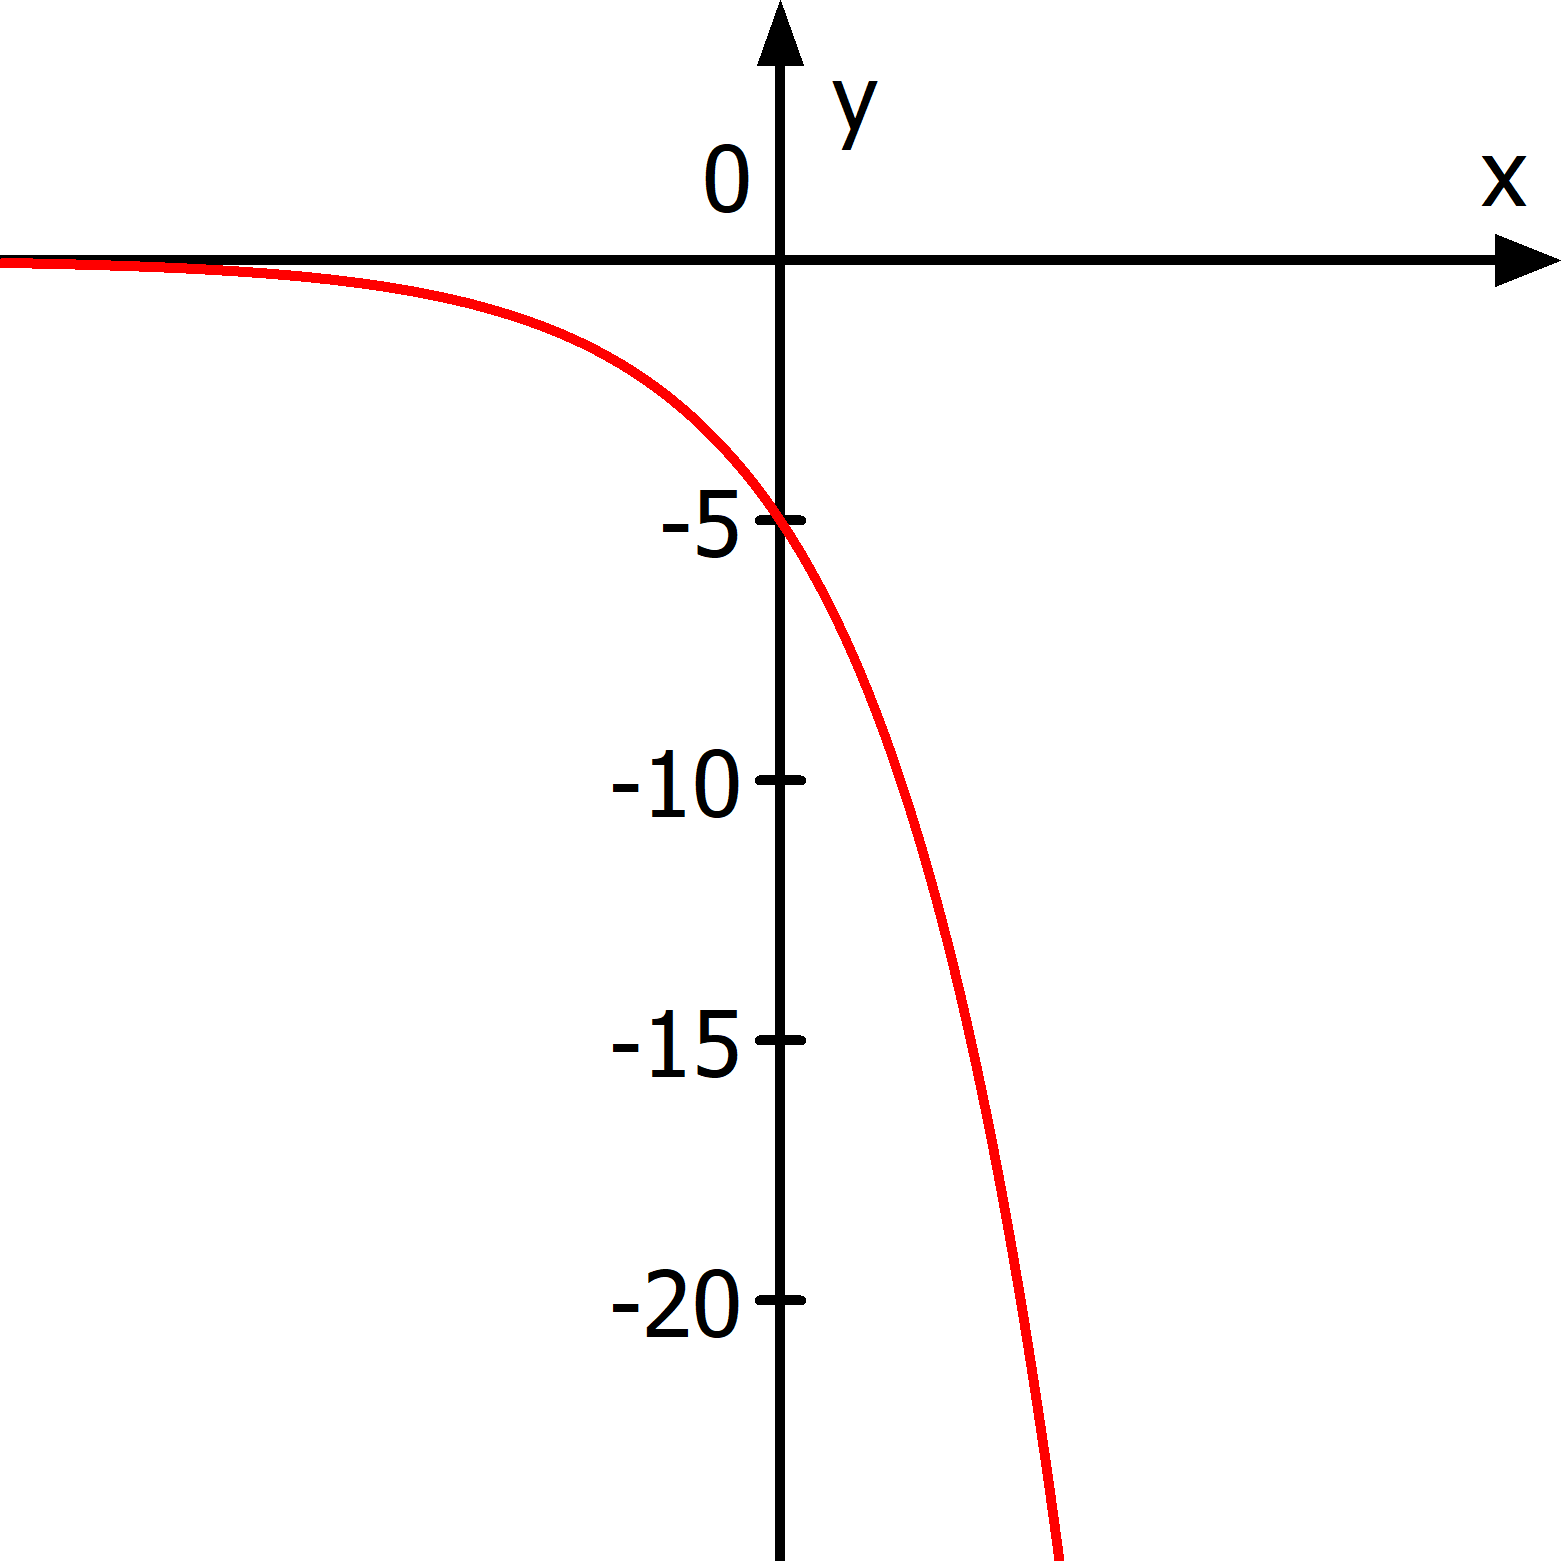
\includegraphics[width=.6\linewidth]{\eFkt/pics/A1x.png}
			\end{enumerate}
		\end{minipage}
	\end{minipage}\\
	%%%%% y bis z
	\begin{minipage}{\textwidth}
		\begin{minipage}[t]{0.49\textwidth}
			\begin{enumerate}[label=\alph*)]
				\setcounter{enumi}{24}
				\item \(f(x)=-0,9e^{-1,1x}\)\\
				Asymptote \(y=0\)\\
				y-Achsenabschnitt: \(f(0)=-0,9\)\\
				Monoton wachsend\\
				\(f(x)\xrightarrow{\hphantom{\ }x\to-\infty\hphantom{\ }}-\infty\)\\
				\(f(x)\xrightarrow{\hphantom{\ }x\to\infty\hphantom{\ }}0\)\\
				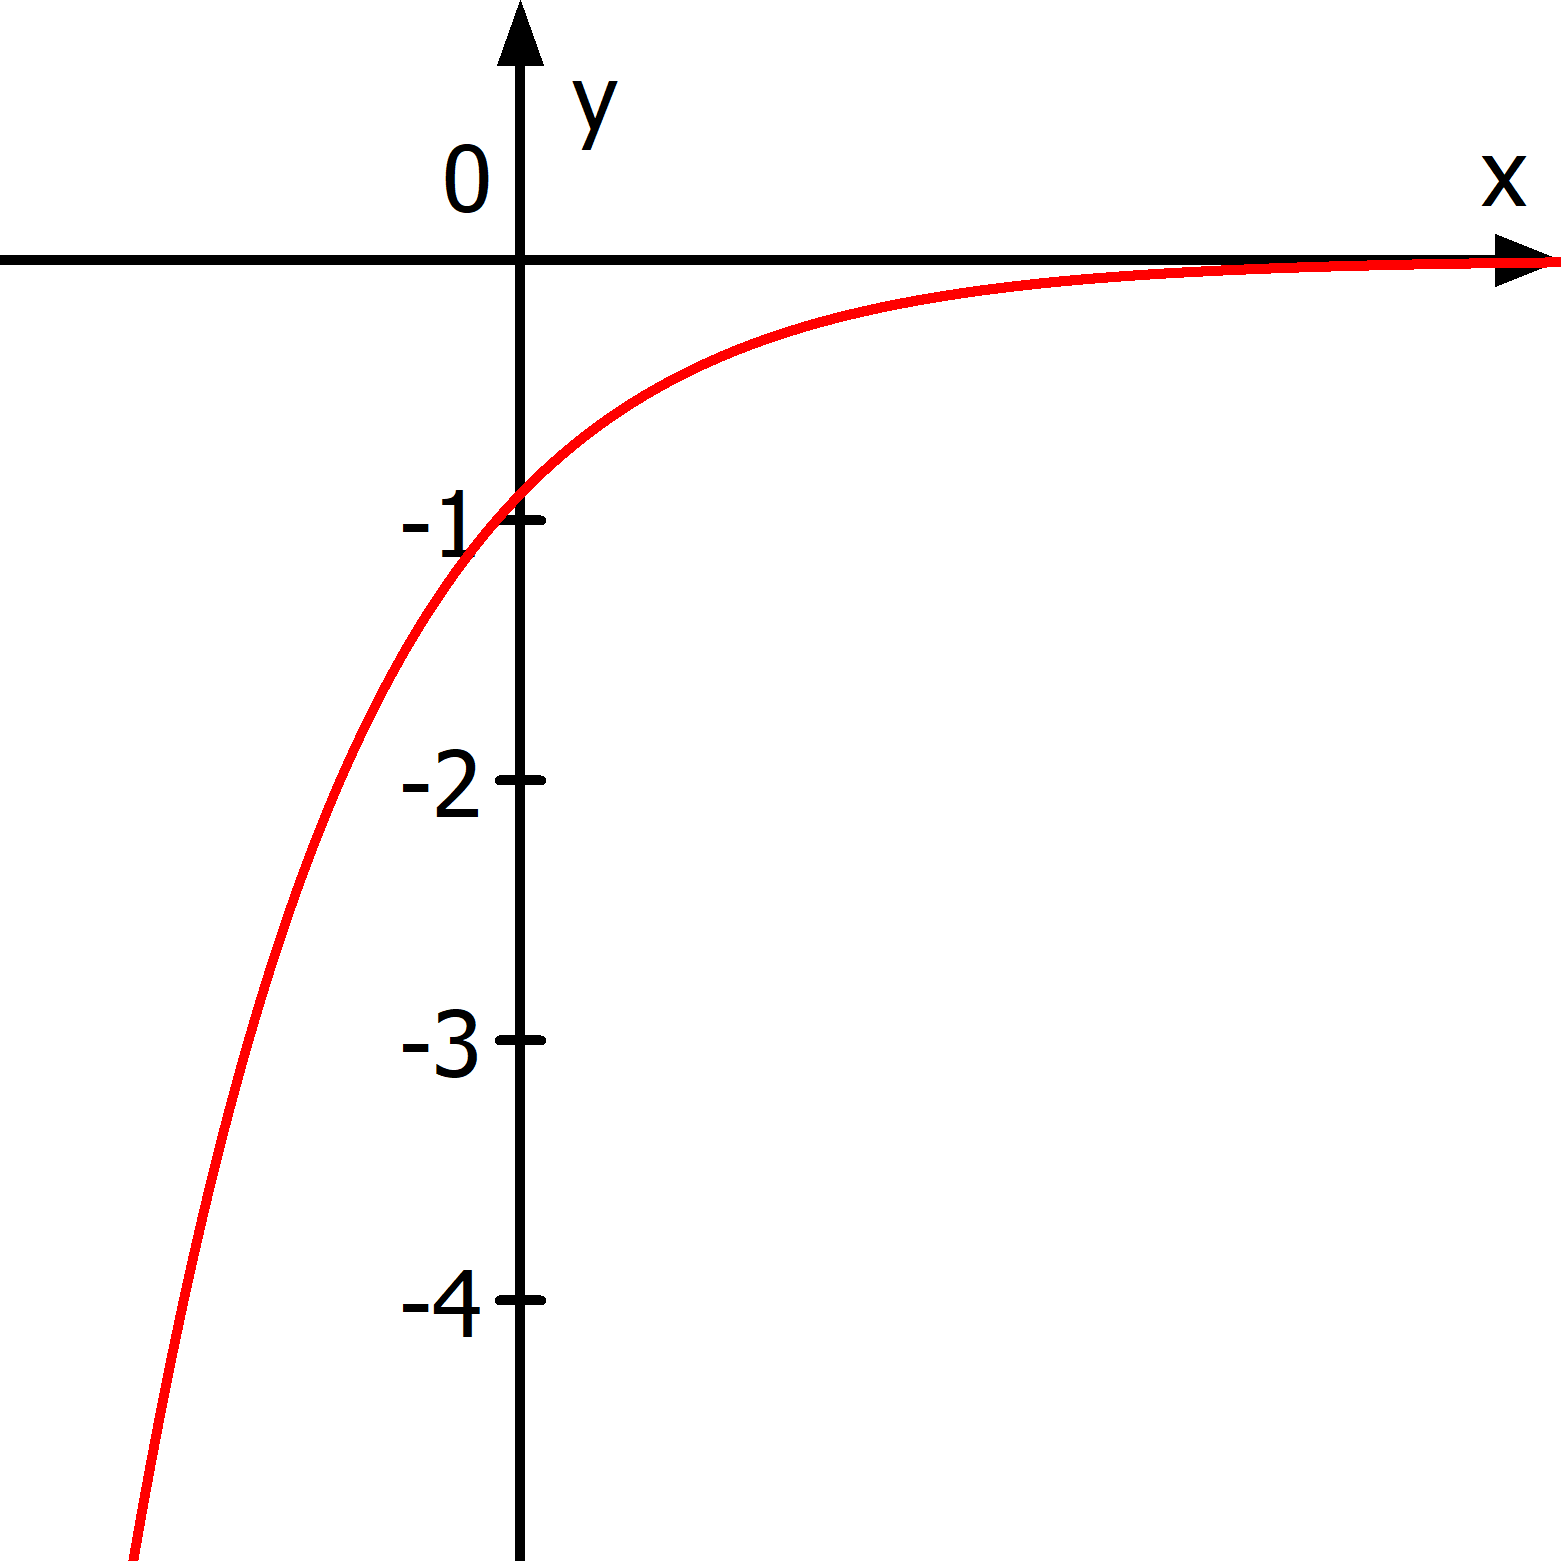
\includegraphics[width=.6\linewidth]{\eFkt/pics/A1y.png}
			\end{enumerate}
		\end{minipage}
		\begin{minipage}[t]{0.49\textwidth}
			\begin{enumerate}[label=\alph*)]
				\setcounter{enumi}{25}
				\item \(f(x)=\frac{11}{6}e^{\frac{8}{7}x}\)\\
				Asymptote \(y=0\)\\
				y-Achsenabschnitt: \(f(0)=\frac{11}{6}\)\\
				Monoton wachsend\\
				\(f(x)\xrightarrow{\hphantom{\ }x\to-\infty\hphantom{\ }}0\)\\
				\(f(x)\xrightarrow{\hphantom{\ }x\to\infty\hphantom{\ }}\infty\)\\
				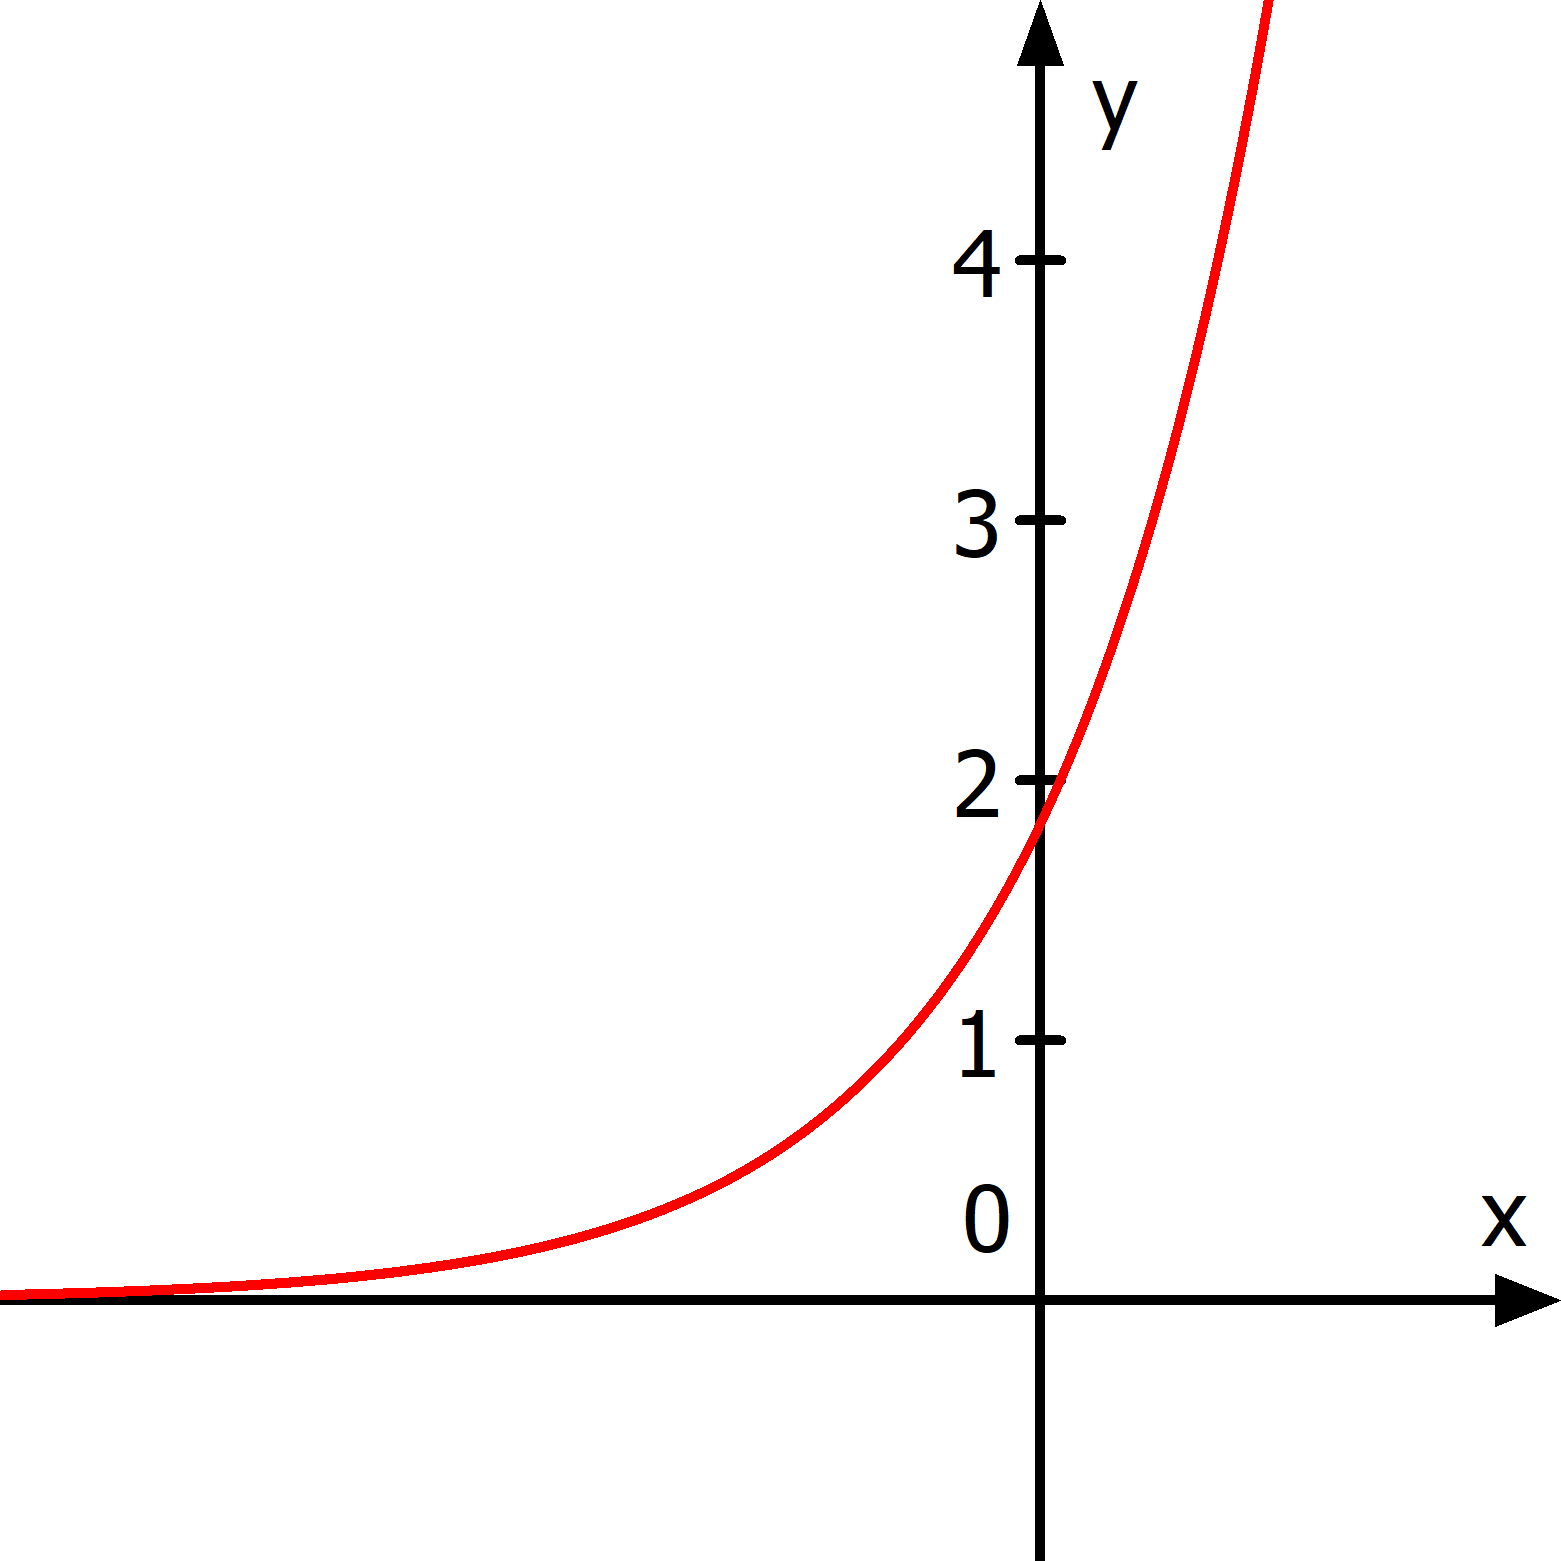
\includegraphics[width=.6\linewidth]{\eFkt/pics/A1z.png}
			\end{enumerate}
		\end{minipage}
	\end{minipage}\\
\end{Answer}
	\newpage
	\cohead{\Large\textbf{Einführung Exponentialfunktionen}}
\fakesubsection{Einführung Exponentialfunktionen}
Die Anzahl der Bakterien in einer Petrischale verdoppelt sich jede Stunde (bis die komplette Schale mit Bakterien bedeckt ist). Zu Beginn sind 10 Bakterien auf der Schale. Vervollständige die Tabelle:\\
\resizebox{\textwidth}{!}{\begin{tabular}{c||c|c|c|c|c|c|c}
		\(x\)&0&1&2&3&4&5&6\\
		\hline
		\multirow{2}{1cm}{\(f(x)\)}&10&20&\textcolor{loes}{40}&\textcolor{loes}{80}&\textcolor{loes}{160}&\textcolor{loes}{320}&\textcolor{loes}{640}\\
		&\textcolor{loes}{\(10\cdot2^0\)}&\textcolor{loes}{\(10\cdot2^1\)}&\textcolor{loes}{\(10\cdot2^2\)}&\textcolor{loes}{\(10\cdot2^3\)}&\textcolor{loes}{\(10\cdot2^4\)}&\textcolor{loes}{\(10\cdot2^5\)}&\textcolor{loes}{\(10\cdot2^6\)}
\end{tabular}}
\vspace{0.3cm}\\
\begin{minipage}{0.50\textwidth}
	\scalebox{2}{\(f(x)= \textcolor{loes}{10\cdot 2^x}\)}\vspace{0.3cm}\\
	Wie viele Bakterien sind nach 20h und nach 100h vorhanden?\\
	\textcolor{loes}{Da \(x\) die Zeit in Stunden angibt, setzt man einfach die angegebenen Werte ein:}
	\begin{align*}
		\textcolor{loes}{f(20)}&\textcolor{loes}{=10\cdot 2^{20}=10.485.760}\\
		\textcolor{loes}{f(100)}&\textcolor{loes}{=10\cdot 2^{100}\approx 1,27\cdot 10^{31}}
	\end{align*}
	Nach wie vielen Stunden waren 8000 Bakterien vorhanden?\\
	\textcolor{loes}{\(f(x)\) gibt die Anzahl an Bakterien nach \(x\) Stunden an. Wir setzen also gleich:}
	\begin{align*}
		\textcolor{loes}{f(x)}&\textcolor{loes}{=8000}\\
		\textcolor{loes}{10\cdot 2^x}&\textcolor{loes}{=8000\,|\,:10}\\
		\textcolor{loes}{2^x}&\textcolor{loes}{=800\,|\,\log_2}\\
		\textcolor{loes}{\Rightarrow x}&\textcolor{loes}{=\log_2(800)\approx 9,64}
	\end{align*}
	\textcolor{loes}{Der Logarithmus erfüllt für Exponentialfunktionen die gleiche Funktion, die die verschiedenen Wurzeln für \(x^2,\ x^3,\) usw. erfüllen.}\\
\end{minipage}
\begin{minipage}{0.49\textwidth}\centering
	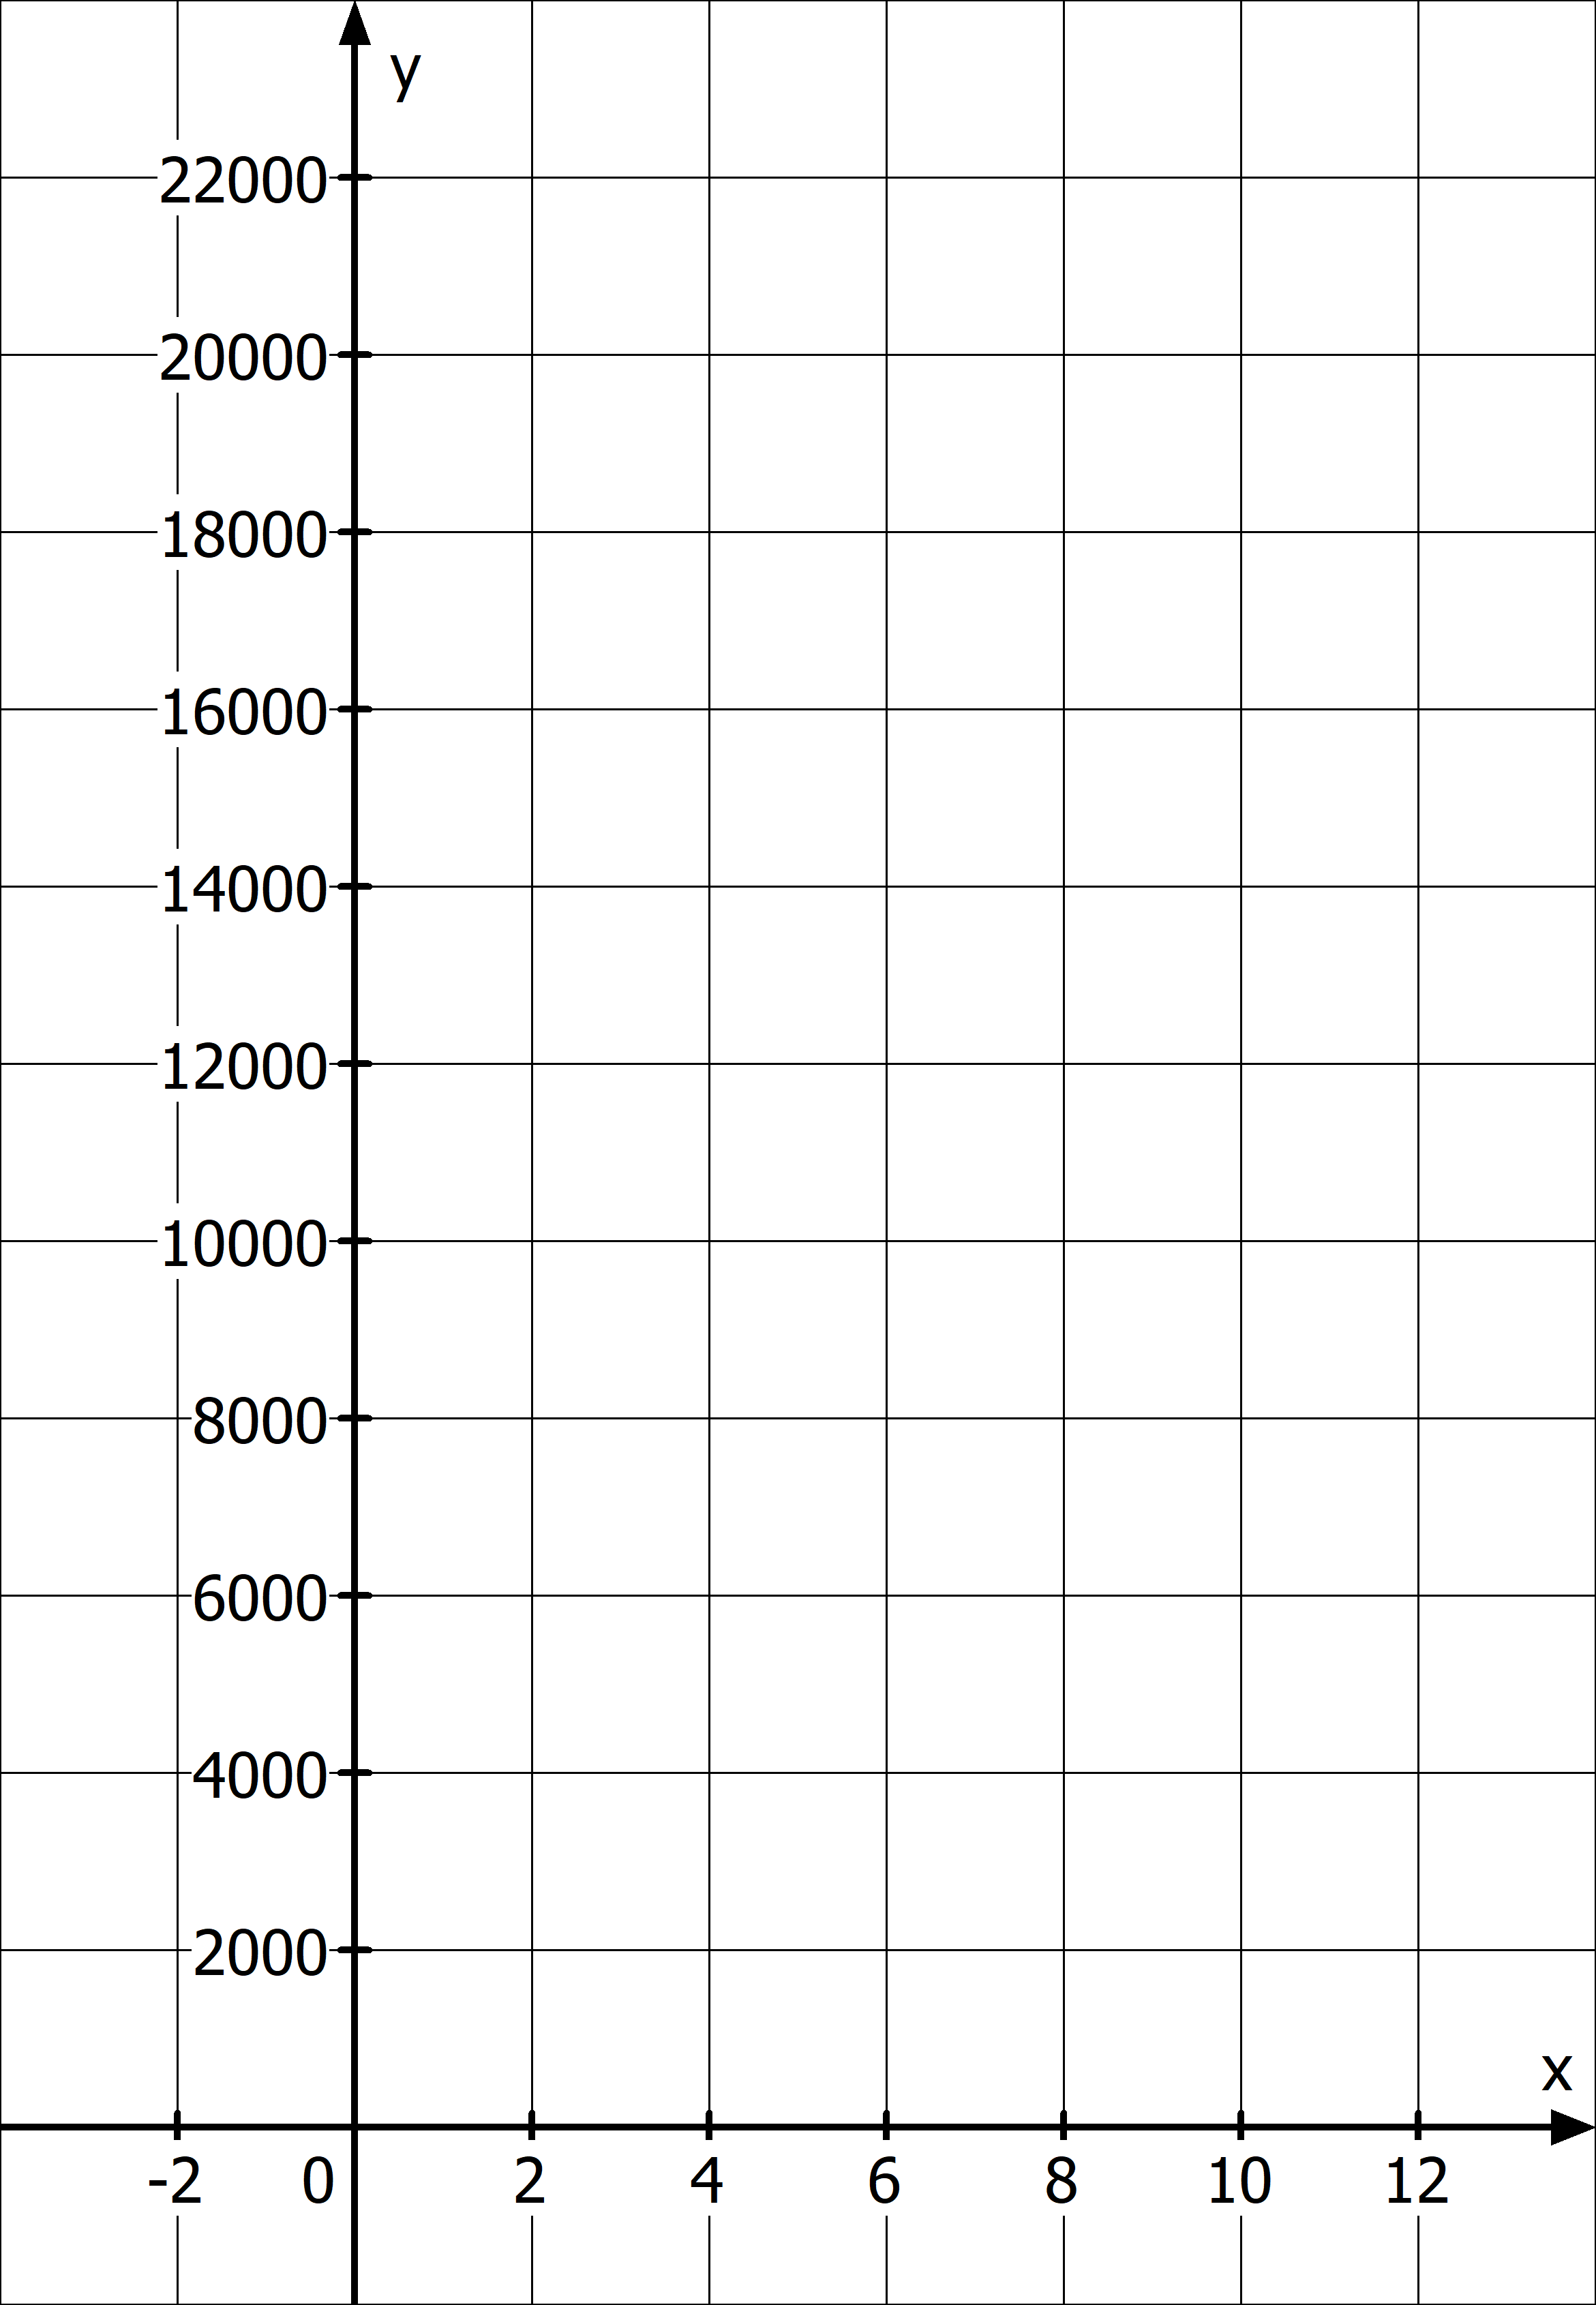
\includegraphics[width=\textwidth]{\eFkt/pics/bakterien_empty.png}
\end{minipage}
Exponentialfunktionen wie \(2^x\) wachsen sehr schnell. Überlegen wir uns zur Illustration wie lange es dauern würde bis die komplette Erde (\(m_{Erde}=6\cdot 10^{24}kg\)) aus Bakterien bestehen würde, falls sie sich unbegrenzt vermehren könnten. 1.000.000.000.000.000 Bakterien wiegen 1g.
\begin{align*}
	\textcolor{loes}{f(x)}&\textcolor{loes}{=6\cdot 10^42}\\
	\textcolor{loes}{10\cdot 2^x}&\textcolor{loes}{=6\cdot 10^42\,|\,:10}\\
	\textcolor{loes}{2^x}&\textcolor{loes}{=6\cdot 10^41\,|\,\log_2}\\
	\textcolor{loes}{\Rightarrow x}&\textcolor{loes}{=\log_2\left( 6\cdot 10^41\right) \approx 138,8}
\end{align*}
\textcolor{loes}{Könnten sich die Bakterien unbegrenzt vermehren, würde es also lediglich \(139h=5,8d\), also nicht ganz 6 Tage, dauern bis die komplette Erde nur aus Bakterien bestehen würde.}
\newpage
%%%%%%%%%%%%%%%%%%%%%%%%%%%%%%%%%%%%%%%%%%%%%%%%%%%%%%%%%%%%%%%%%%%%%%%%%%%%%%%%%%%%%%%%%%%%%%%%%%%%%%
Das Isotop \(^{207}\)Ra hat eine Halbwertszeit von ca. 1s, d.h. dass innerhalb einer Sekunde die Hälfte des radioaktiven Materials in andere Elemente zerfallen ist. Zu Beginn sind 8g Radium vorhanden. Vervollständige die Tabelle:\\
\resizebox{\textwidth}{!}{\begin{tabular}{c||c|c|c|c|c|c|c}
		\(x\)&0&1&2&3&4&5&6\\
		\hline
		\multirow{2}{1cm}{\(f(x)\)}
		&8
		&4
		&\textcolor{loes}{2}
		&\textcolor{loes}{1}
		&\textcolor{loes}{\(\frac{1}{2}\)}
		&\textcolor{loes}{\(\frac{1}{4}\)}
		&\textcolor{loes}{\(\frac{1}{8}\)}\\
		&\textcolor{loes}{\(8\cdot\left(\frac{1}{2}\right)^0\)}
		&\textcolor{loes}{\(8\cdot\left(\frac{1}{2}\right)^1\)}
		&\textcolor{loes}{\(8\cdot\left(\frac{1}{2}\right)^2\)}
		&\textcolor{loes}{\(8\cdot\left(\frac{1}{2}\right)^3\)}
		&\textcolor{loes}{\(8\cdot\left(\frac{1}{2}\right)^4\)}
		&\textcolor{loes}{\(8\cdot\left(\frac{1}{2}\right)^5\)}
		&\textcolor{loes}{\(8\cdot\left(\frac{1}{2}\right)^6\)}
\end{tabular}}
\vspace{0.3cm}\\
\begin{minipage}{0.39\textwidth}
	\scalebox{2}{\(f(x)= \textcolor{loes}{8\cdot \left(\frac{1}{2}\right)^x}\)}\vspace{0.3cm}\\
	Wie viel \(g\) Radium sind nach 10s noch vorhanden, wie viel nach 1min?\\
	\textcolor{loes}{Da \(x\) die Zeit in Sekunden angibt, setzt man einfach die angegebenen Werte ein:}
	\begin{align*}
		\textcolor{loes}{f(10)}&\textcolor{loes}{=8\cdot \left(\frac{1}{2}\right)^{10}=\frac{1}{128}\approx 0,00781}\\
		\textcolor{loes}{f(60)}&\textcolor{loes}{=8\cdot \left(\frac{1}{2}\right)^{60}=\frac{1}{128}\approx 6,94\cdot10^{-18}}
	\end{align*}
	\vfill
\end{minipage}
\begin{minipage}{0.6\textwidth}\centering
	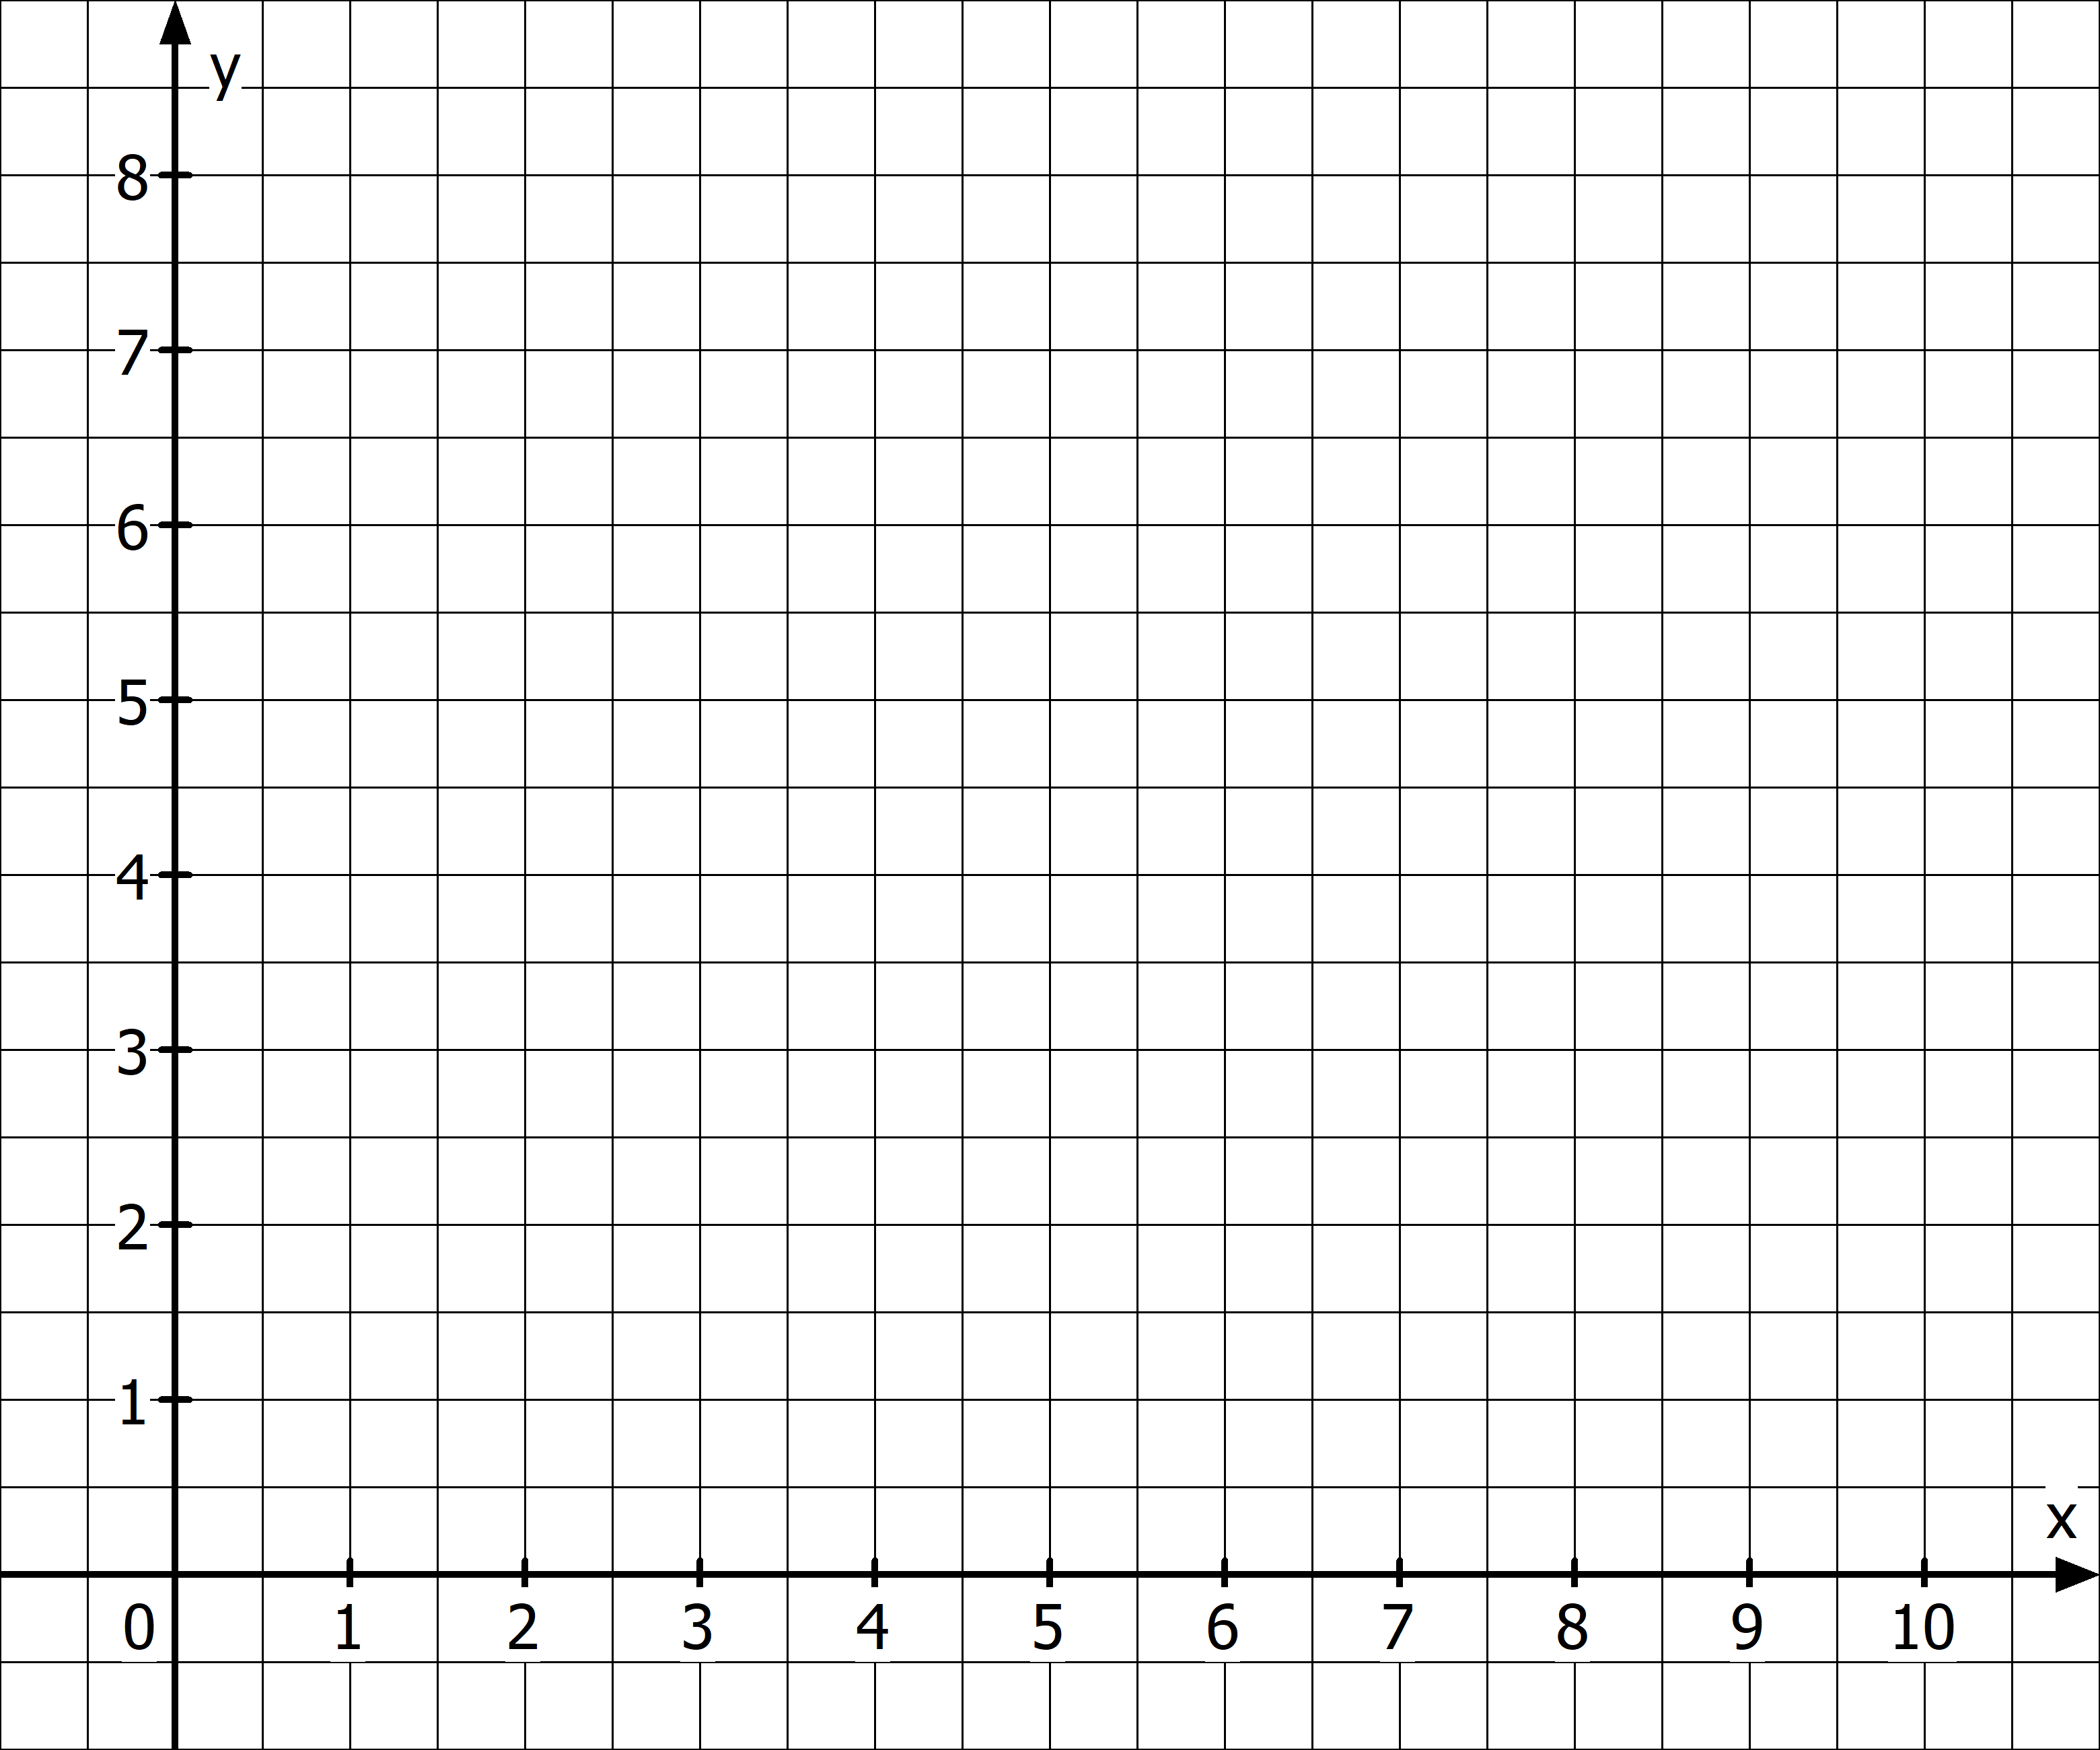
\includegraphics[width=\textwidth]{\eFkt/pics/radium_empty.png}
\end{minipage}\vspace{0.3cm}\\
Nach wie vielen Sekunden waren noch 0,3g Radium vorhanden?\\
\textcolor{loes}{\(f(x)\) gibt die Masse des Radiums in \(g\) nach \(x\) Sekunden an. Wir setzen also gleich:}
\begin{align*}
	\textcolor{loes}{f(x)}&\textcolor{loes}{=0,3}\\
	\textcolor{loes}{8\cdot \left(\frac{1}{2}\right)^x}&\textcolor{loes}{=0,3\,|\,:8}\\
	\textcolor{loes}{\left(\frac{1}{2}\right)^x}&\textcolor{loes}{=\frac{3}{80}\,|\,\log_{\frac{1}{2}}}\\
	\textcolor{loes}{\Rightarrow x}&\textcolor{loes}{=\log_{\frac{1}{2}}\left(\frac{3}{80}\right) \approx 4,74}
\end{align*}
Wie lange würde es dauern bis die Masse des Radiums die eines Bakteriums entspricht?
\begin{align*}
	\textcolor{loes}{f(x)}&\textcolor{loes}{=10^{-15}}\\
	\textcolor{loes}{8\cdot \left(\frac{1}{2}\right)^x}&\textcolor{loes}{=10^{-15}\,|\,:8}\\
	\textcolor{loes}{\left(\frac{1}{2}\right)^x}&\textcolor{loes}{=1,25\cdot 10^{-16}\,|\,\log_{\frac{1}{2}}}\\
	\textcolor{loes}{\Rightarrow x}&\textcolor{loes}{=\log_{\frac{1}{2}}\left(1,25\cdot 10^{-16}\right) \approx 52,8}
\end{align*}
\textcolor{loes}{Es dauert also nicht mal ganz eine Minute bis das Radium fast verschwunden ist.}
	\newpage
	% !TeX root = ../../Skript.tex
\cohead{\Large\textbf{Punktprobe}}
\fakesubsection{Punktprobe}
Ein besserer Begriff für Punktprobe wäre Punkteinsetzen. Sind eine Funktion \(f(x)\) und ein Punkt \(P(x_P\vert y_P)\) gegeben, so kann man prüfen, ob das Schaubild von \(f(x)\) durch den Punkt verläuft, indem man den Punkt einsetzt:
\begin{tcolorbox}
	\centering
	\textcolor{loestc}{\(f(x_P)\overset{?}{=}y_P\)}
\end{tcolorbox}

\textbf{Beispiel:}

Gegeben sind die Funktion \(f(x)=2x-1\) und zwei Punkt \(P(\textcolor{red}{2}\vert\textcolor{blue}{3})\) sowie \(Q(\textcolor{red}{0}\vert\textcolor{blue}{4})\).

\(P:\ \textcolor{loes}{f(2)=2\cdot 2-1=4-1=3=3}\)

Der Punkt \(P\) liegt also auf dem Schaubild von \(f(x)\).

\(Q:\ \textcolor{loes}{f(0)=2\cdot 0-1=0-1=-1\neq4}\)

Der Punkt \(Q\) liegt also nicht auf dem Schaubild von \(f(x)\).

In den meisten Fällen wird eine Punktprobe verwendet, um Teile einer Funktionsgleichung zu bestimmen.

\begin{minipage}{\textwidth}
\adjustbox{valign=t}{\begin{minipage}{0.5\textwidth}
	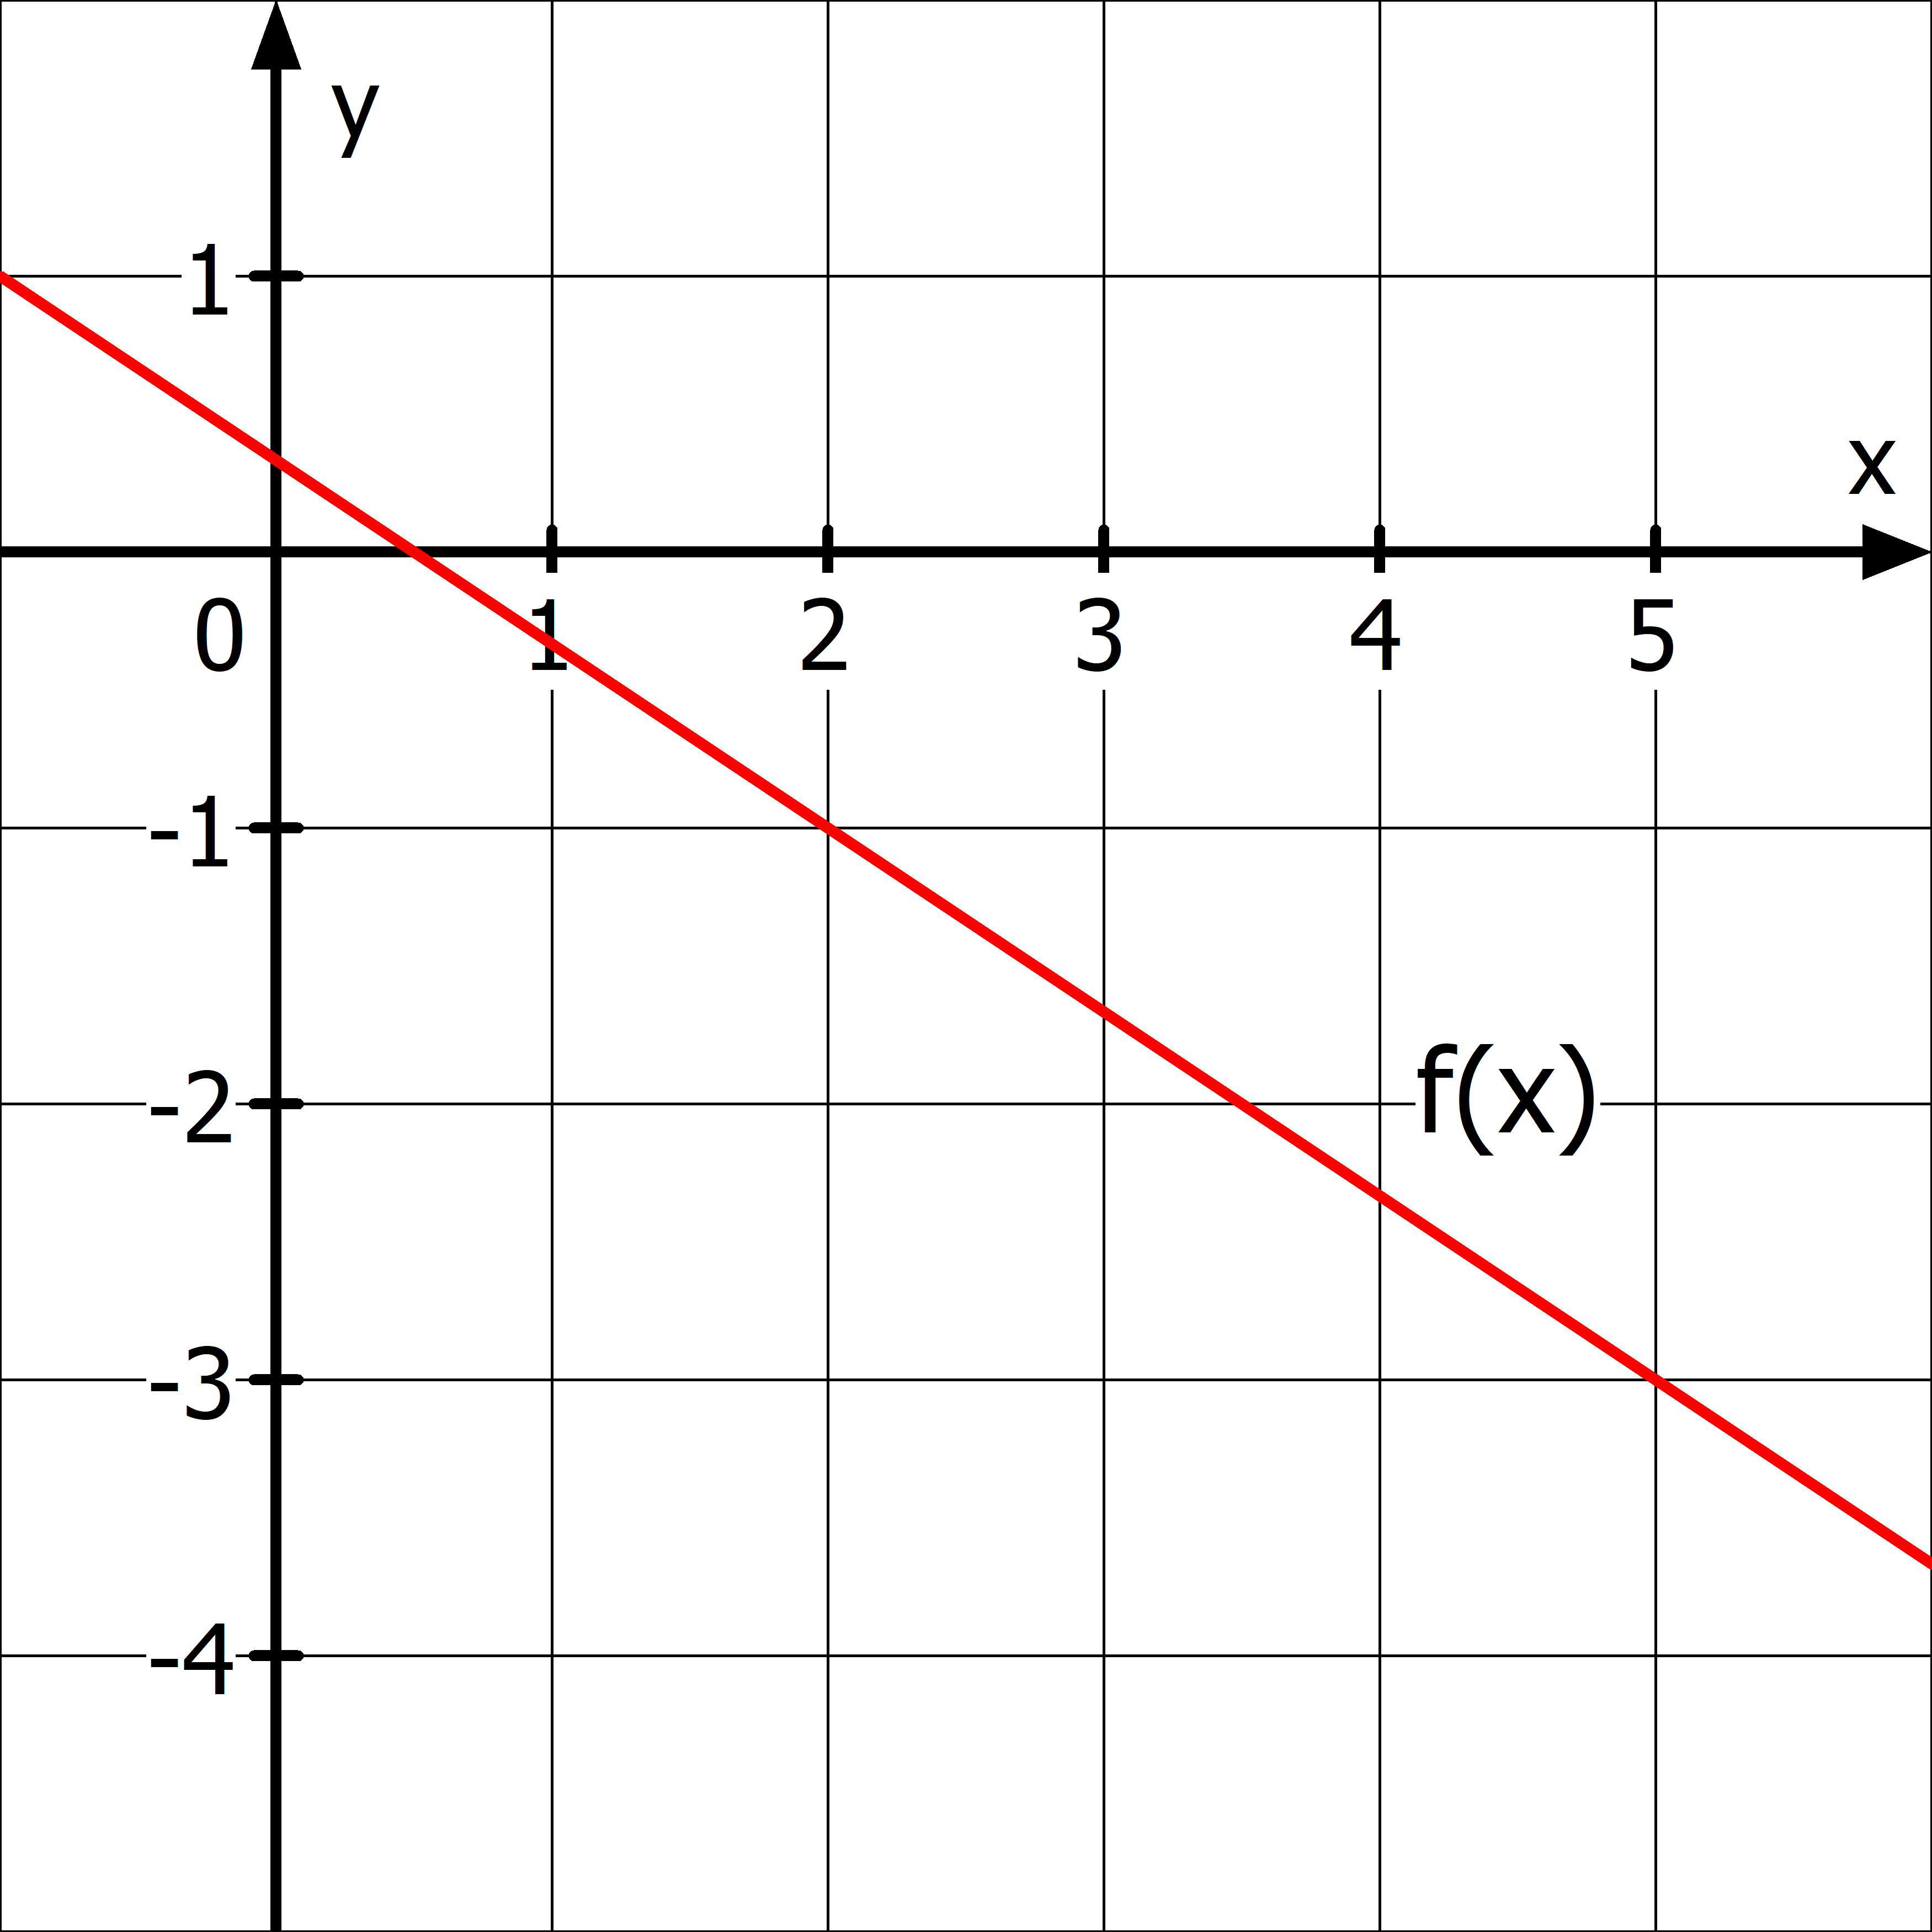
\includegraphics[width=0.90\textwidth]{\linFkt/pics/punktprobe.png}
\end{minipage}}%
\adjustbox{valign=t}{\begin{minipage}{0.5\textwidth}
	Im nebenstehenden Beispiel lässt sich die Steigung der Geraden \(f(x)=mx+b\) leicht über ein Steigungsdreieck bestimmen: \(\textcolor{ForestGreen}{m=-\tfrac{2}{3}}\). Der y-Achsenabschnitt kann leider nicht exakt abgelesen werden. Wir lesen daher einen beliebigen Punkt ab, z.B. \(P(\textcolor{red}{2}\vert\textcolor{blue}{-1})\) und führen mit diesem Punkt eine Punktprobe durch:
	\begin{align*}
		f(\textcolor{red}{2})&=\textcolor{blue}{-1}\\
		\textcolor{loes}{-\dfrac{2}{3}\cdot2+b}&\textcolor{loes}{\;=-1\ \vert+\dfrac{4}{3}}\\
		\textcolor{loes}{b}&\textcolor{loes}{\;=\dfrac{1}{3}}
	\end{align*}

\end{minipage}}%
\end{minipage}
\begin{Exercise}[title={Prüfe, ob die Punkte auf dem Schaubild der Funktion liegen}, label=punktprobeA1]
	\begin{enumerate}[label=\alph*)]
		\item \(f(x)=-x+2\qquad P(2\vert3)\text{ und }Q(-2\vert4)\)
		\item \(g(x)=\dfrac{4}{5}x-1\qquad R(5\vert3)\text{ und }S(10\vert-1)\)
	\end{enumerate}
\end{Exercise}
\begin{Exercise}[title={Bestimme die Funktionsgleichung}, label=punktprobeA2]
	\begin{enumerate}[label=\alph*)]
		\item Das Schaubild der Funktion \(f(x)=2x+b\) verläuft durch den Punkt \(P(2\vert3)\).
		\item Das Schaubild der Funktion \(g(x)=mx-1\) verläuft durch den Punkt \(Q(-2\vert6)\).
		\item Das Schaubild der Funktion \(h(x)=mx+b\) verläuft durch die Punkte \(R_1(2\vert3)\) und \(R_2(4\vert-1)\).
		\item Das Schaubild der Funktion \(i(x)=mx+b\) verläuft durch die Punkte \(S_1(-1\vert-2)\) und \(S_2(5\vert7)\).
	\end{enumerate}
\end{Exercise}
\newpage
\begin{Answer}[ref=punktprobeA1]

	\begin{minipage}{0.5\textwidth}
		\begin{enumerate}[label=\alph*)]
			\item \(f(\textcolor{red}{2})=-\textcolor{red}{2}+2=0\neq\textcolor{blue}{3}\)

			\(P\) liegt nicht auf dem Schaubild von \(f(x)\)

			\(f(\textcolor{red}{-2})=-\left(\textcolor{red}{-2}\right)+2=\textcolor{blue}{4}\)

			\(Q\) liegt auf dem Schaubild von \(f(x)\)
		\end{enumerate}
	\end{minipage}%
	\begin{minipage}{0.5\textwidth}
		\begin{enumerate}[label=\alph*)]
			\setcounter{enumi}{1}
			\item \(g(\textcolor{red}{5})=\tfrac{4}{5}\cdot\textcolor{red}{5}-1=\textcolor{blue}{3}\)

			\(R\) liegt auf dem Schaubild von \(g(x)\)

			\(g(\textcolor{red}{10})=\tfrac{4}{5}\cdot\textcolor{red}{10}-1=7\neq\textcolor{blue}{-1}\)

			\(S\) liegt nicht auf dem Schaubild von \(g(x)\)
		\end{enumerate}
	\end{minipage}%
\end{Answer}
\vspace{1cm}
\begin{Answer}[ref=punktprobeA2]

	\begin{minipage}[t]{0.5\textwidth}
		\begin{enumerate}[label=\alph*)]
			\item Punktprobe mit \(P(\textcolor{red}{2}\vert\textcolor{blue}{3})\)
			\begin{align*}
				f(\textcolor{red}{2})&=\textcolor{blue}{3}\\
				2\cdot\textcolor{red}{2})+b&=\textcolor{blue}{3}\ \vert-4\\
				b&=-1\\
				\Rightarrow f(x)&=2x-1
			\end{align*}
			\item Punktprobe mit \(Q(\textcolor{red}{-2}\vert\textcolor{blue}{6})\)
			\begin{align*}
				g(\textcolor{red}{-2})&=\textcolor{blue}{6}\\
				m\cdot\left(\textcolor{red}{-2}\right)-1&=\textcolor{blue}{6}\ \vert+1\\
				\textcolor{red}{-2}m&=7\ \vert\left(\cdot -\tfrac{1}{2}\right)\\
				m&=-\dfrac{7}{2}\\
				\Rightarrow g(x)&=-\dfrac{7}{2}x-1
			\end{align*}
		\end{enumerate}
	\end{minipage}%
	\begin{minipage}[t]{0.5\textwidth}
		\begin{enumerate}[label=\alph*)]
			\setcounter{enumi}{2}
			\item Bestimmen der Steigung \(m\) mit Hilfe der Punkte \(R_1(\textcolor{red}{2}\vert\textcolor{blue}{3})\) und \(R_2(\textcolor{ForestGreen}{4}\vert\textcolor{YellowOrange}{-1})\):
			\begin{align*}
				m=\dfrac{\textcolor{YellowOrange}{-1}-\textcolor{blue}{3}}{\textcolor{ForestGreen}{4}-\textcolor{red}{2}}=-2
			\end{align*}
			Punktprobe mit \(R_1(\textcolor{red}{2}\vert\textcolor{blue}{3})\) (oder \(R_2\))
			\begin{align*}
				h(\textcolor{red}{2})&=\textcolor{blue}{3}\\
				-2\cdot\textcolor{red}{2}+b&=\textcolor{blue}{3}\ \vert +4\\
				b&=7\\
				\Rightarrow h(x)&=-2x+7
			\end{align*}
			\item Bestimmen der Steigung \(m\) mit Hilfe der Punkte \(S_1(\textcolor{red}{-1}\vert\textcolor{blue}{-2})\) und \(S_2(\textcolor{ForestGreen}{5}\vert\textcolor{YellowOrange}{7})\):
			\begin{align*}
				m=\dfrac{\textcolor{YellowOrange}{7}-\left(\textcolor{blue}{-2}\right)}{\textcolor{ForestGreen}{5}-\left(\textcolor{red}{-1}\right)}=-\dfrac{3}{2}
			\end{align*}
			Punktprobe mit \(S_2(\textcolor{ForestGreen}{5}\vert\textcolor{YellowOrange}{7})\) (oder \(S_1\))
			\begin{align*}
				i(\textcolor{ForestGreen}{5})&=\textcolor{YellowOrange}{7}\\
				\dfrac{3}{2}\cdot\textcolor{ForestGreen}{5}+b&=\textcolor{YellowOrange}{7}\ \vert -\tfrac{15}{2}\\
				b&=-\dfrac{1}{2}\\
				\Rightarrow i(x)&=\dfrac{3}{2}x+-\dfrac{1}{2}
			\end{align*}
		\end{enumerate}
	\end{minipage}%
\end{Answer}
	\newpage
	% !TeX root = ../../Skript.tex
\cohead{\Large\textbf{Nullstellen}}
\fakesubsection{Nullstellen}
In der Mathematik unterscheidet man grundsätzlich zwischen Stellen und Punkten. Stellen sind x-Werte während Punkte einen x-Wert und einen y-Wert haben. Die Nullstellen (abgekürzt NST) sind die Stellen, an denen die Funktion die x-Achse schneidet.Oder anders ausgedrückt, die NST sind die Stellen, an denen der Funktionswert bzw. y-Wert Null ist:
\begin{tcolorbox}
	\centering
	\textcolor{loestc}{\(f(x)=0\)}
\end{tcolorbox}

\textbf{Beispiel:}

\adjustbox{valign=t}{\begin{minipage}{0.55\textwidth}
	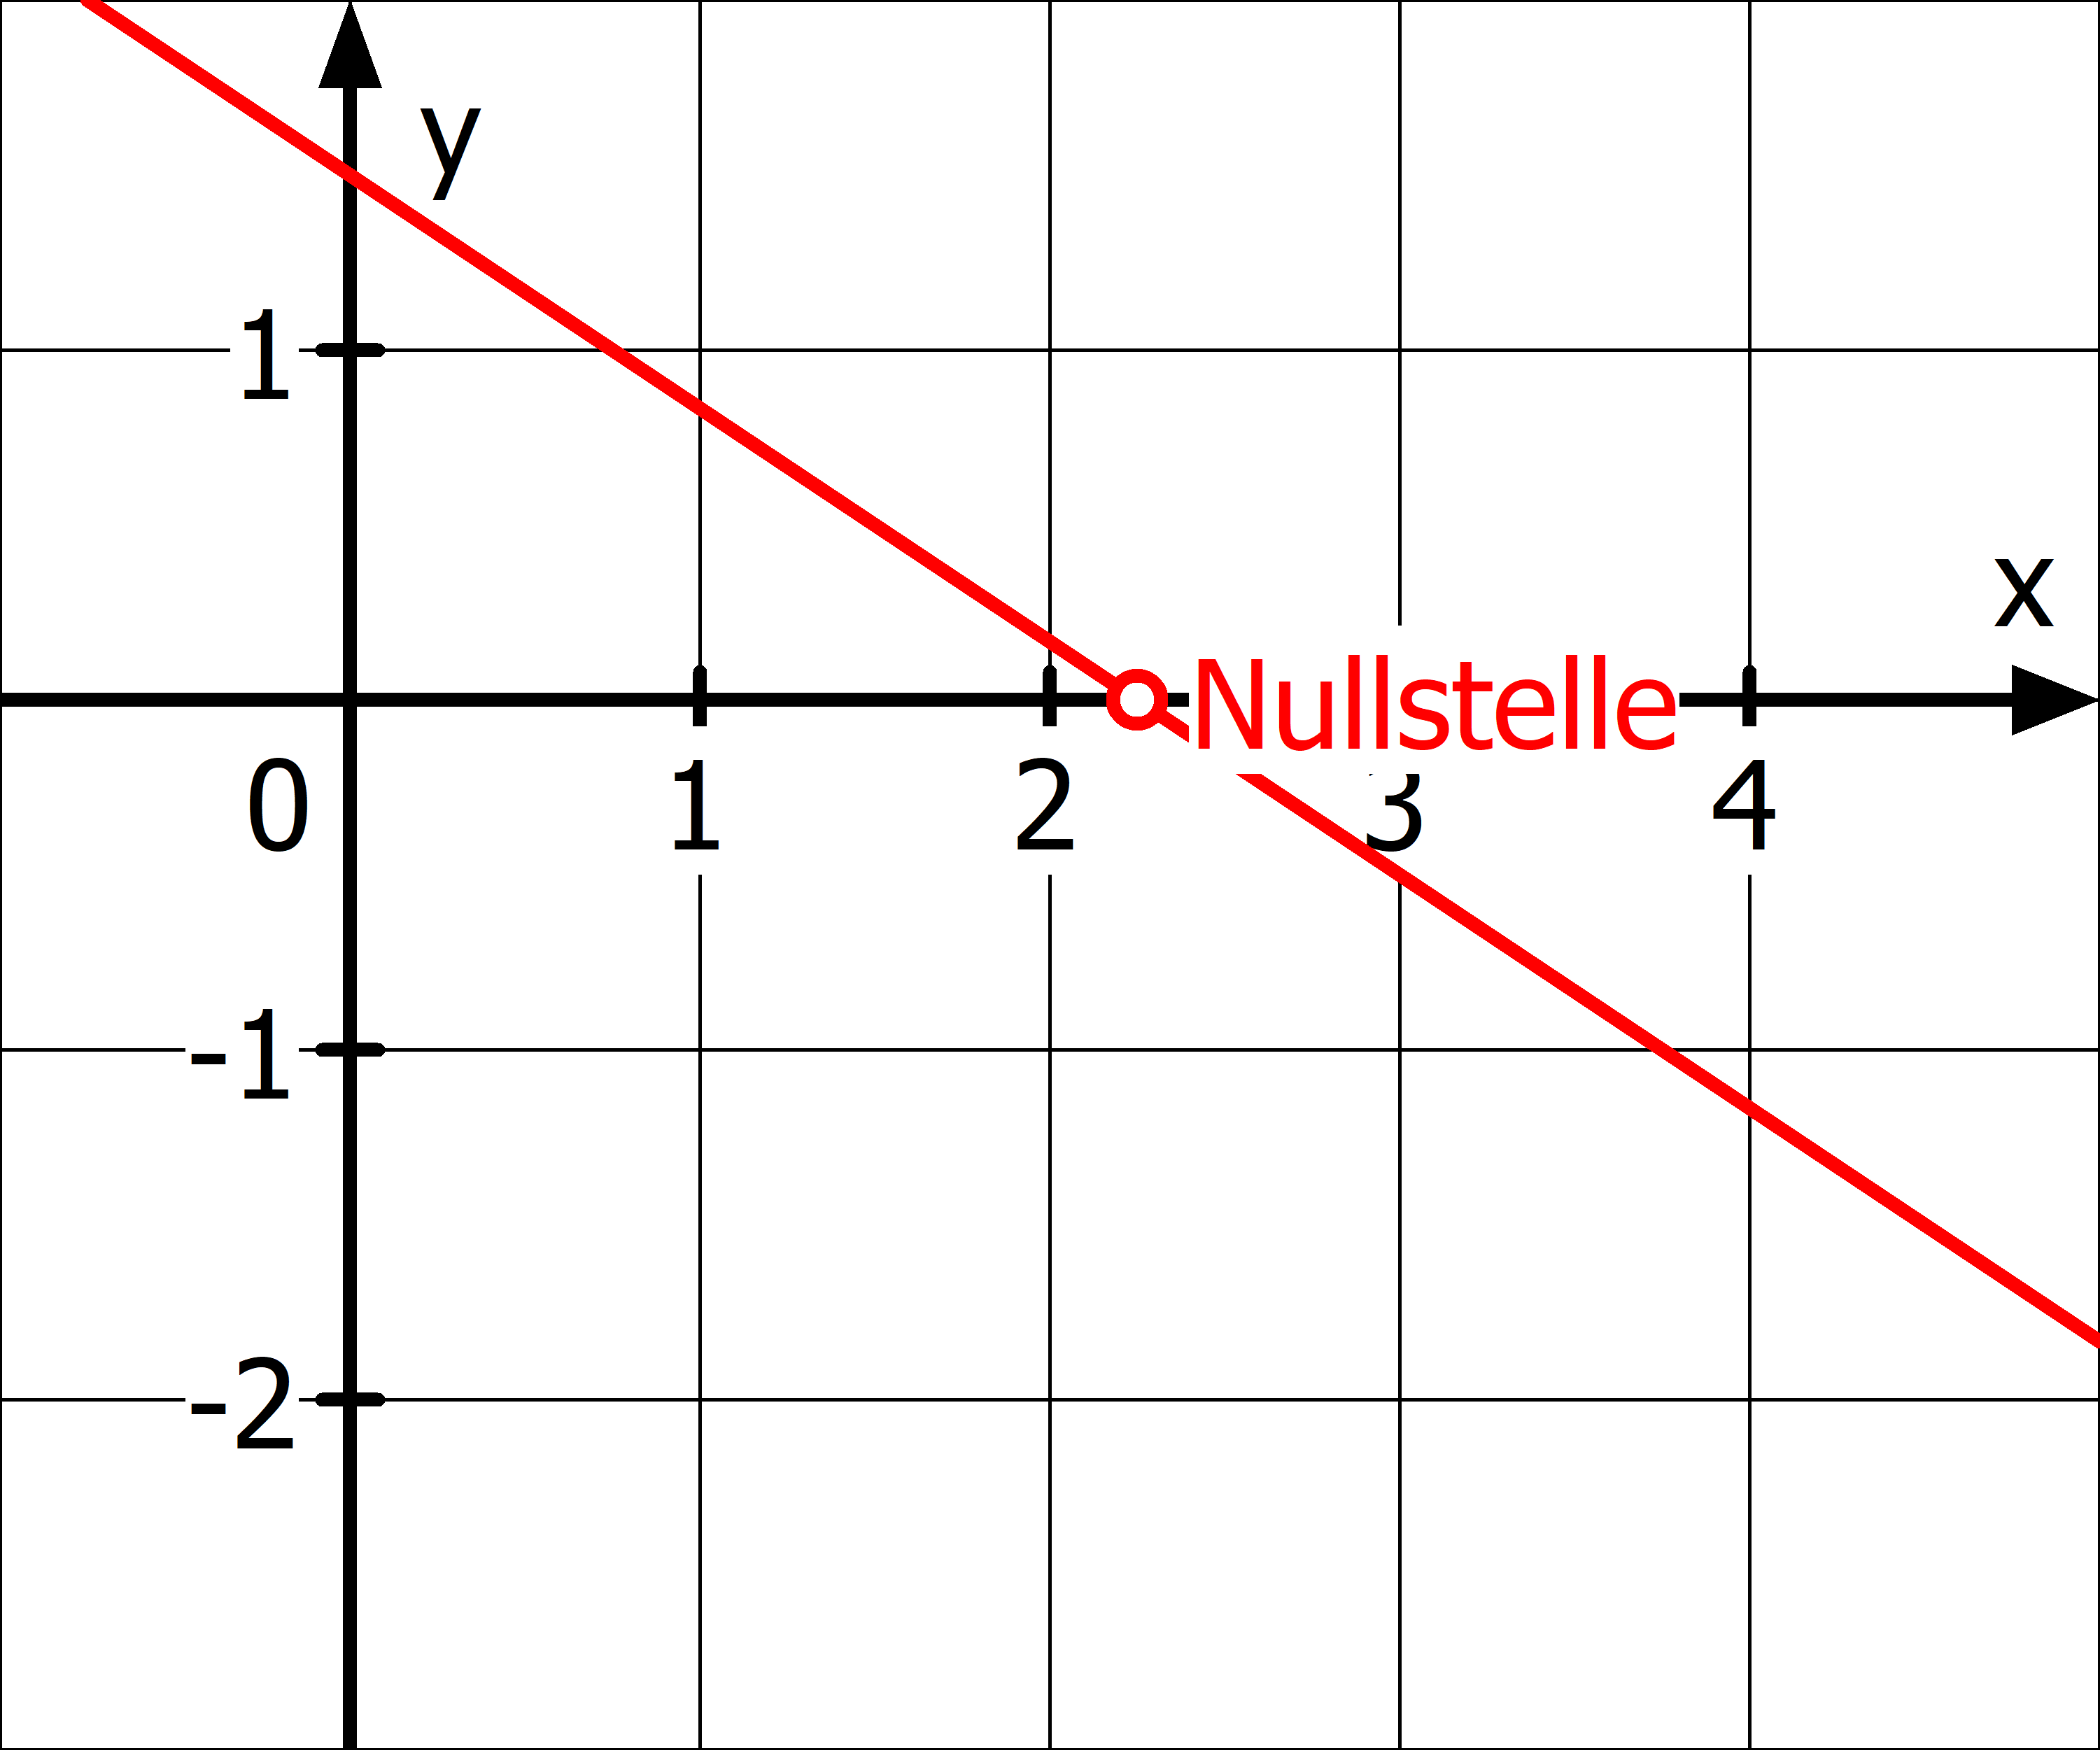
\includegraphics[width=0.95\textwidth]{\linFkt/pics/nullstelle.png}
\end{minipage}}%
\adjustbox{valign=t}{\begin{minipage}{0.45\textwidth}
	Gegeben ist die Funktion \(f(x)=-\tfrac{2}{3}x+\tfrac{3}{2}\).
	Im Schaubild kann man die Nullstelle ungefähr ablesen: \(x_0\approx 2,2\).\\
	Um den exakten Wert zu erhalten, muss man folgende Gleichung lösen:
	\begin{align*}
		\textcolor{loes}{f(x)}&\textcolor{loes}{=0}\\
		\textcolor{loes}{-\tfrac{2}{3}x+\tfrac{3}{2}}&\textcolor{loes}{=0\ \vert-\dfrac{3}{2}}\\
		\textcolor{loes}{-\tfrac{2}{3}x}&\textcolor{loes}{=-\tfrac{3}{2}\ \vert\cdot\left(-\tfrac{3}{2}\right)}\\
		\textcolor{loes}{\Rightarrow x_0}&\textcolor{loes}{=\tfrac{9}{4}=2,25}
	\end{align*}
\end{minipage}}%

\begin{Exercise}[title={Bestimme die Nullstellen}, label=nullstellenA1]\ \\
	\begin{minipage}{0.5\textwidth}
		\begin{enumerate}[label=\alph*)]
			\item \(f_1(x)=3x-9\)
			\item \(f_2(x)=-2x-10\)
			\item \(f_3(x)=\frac{2}{3}x+4\)
			\item \(f_4(x)=-\frac{3}{4}x+12\)
			\item \(f_5(x)=\frac{5}{2}x+\frac{10}{3}\)
		\end{enumerate}
	\end{minipage}%
	\begin{minipage}{0.5\textwidth}
		\begin{enumerate}[label=\alph*)]
			\setcounter{enumi}{5}
			\item \(f_6(x)=-0,5x-3,2\)
			\item \(f_7(x)=-8+2x\)
			\item \(f_8(x)=\frac{5}{7}-\frac{15}{14}x\)
			\item \(f_9(x)=3(2x-5)\)
			\item \(f_{10}(x)=\frac{1}{3}\left(6x-5\right)+\frac{5}{6}\)
		\end{enumerate}
	\end{minipage}%
\end{Exercise}\vspace{0,5cm}
\begin{Answer}[ref=nullstellenA1]\\
	\begin{minipage}{0.5\textwidth}
		\begin{enumerate}[label=\alph*)]
			\item \(x_0=3\)
			\item \(x_0=-5\)
			\item \(x_0=-6\)
			\item \(x_0=16\)
			\item \(x_0=-\frac{4}{3}\)
		\end{enumerate}
	\end{minipage}%
	\begin{minipage}{0.5\textwidth}
		\begin{enumerate}[label=\alph*)]
			\setcounter{enumi}{5}
			\item \(x_0=-6,4\)
			\item \(x_0=4\)
			\item \(x_0=\frac{2}{3}\)
			\item \(x_0=\frac{5}{2}\)
			\item \(x_0=\frac{5}{12}\)
		\end{enumerate}
	\end{minipage}%
\end{Answer}
	\newpage
	\cohead{\Large\textbf{Gegenseitige Lage von Geraden}}
\fakesubsection{Gegenseitige Lage von Geraden}

\begin{tabular}{c|c}
	\multicolumn{2}{c}{\Large\textcolor{loes}{Parallele Geraden}} \\ 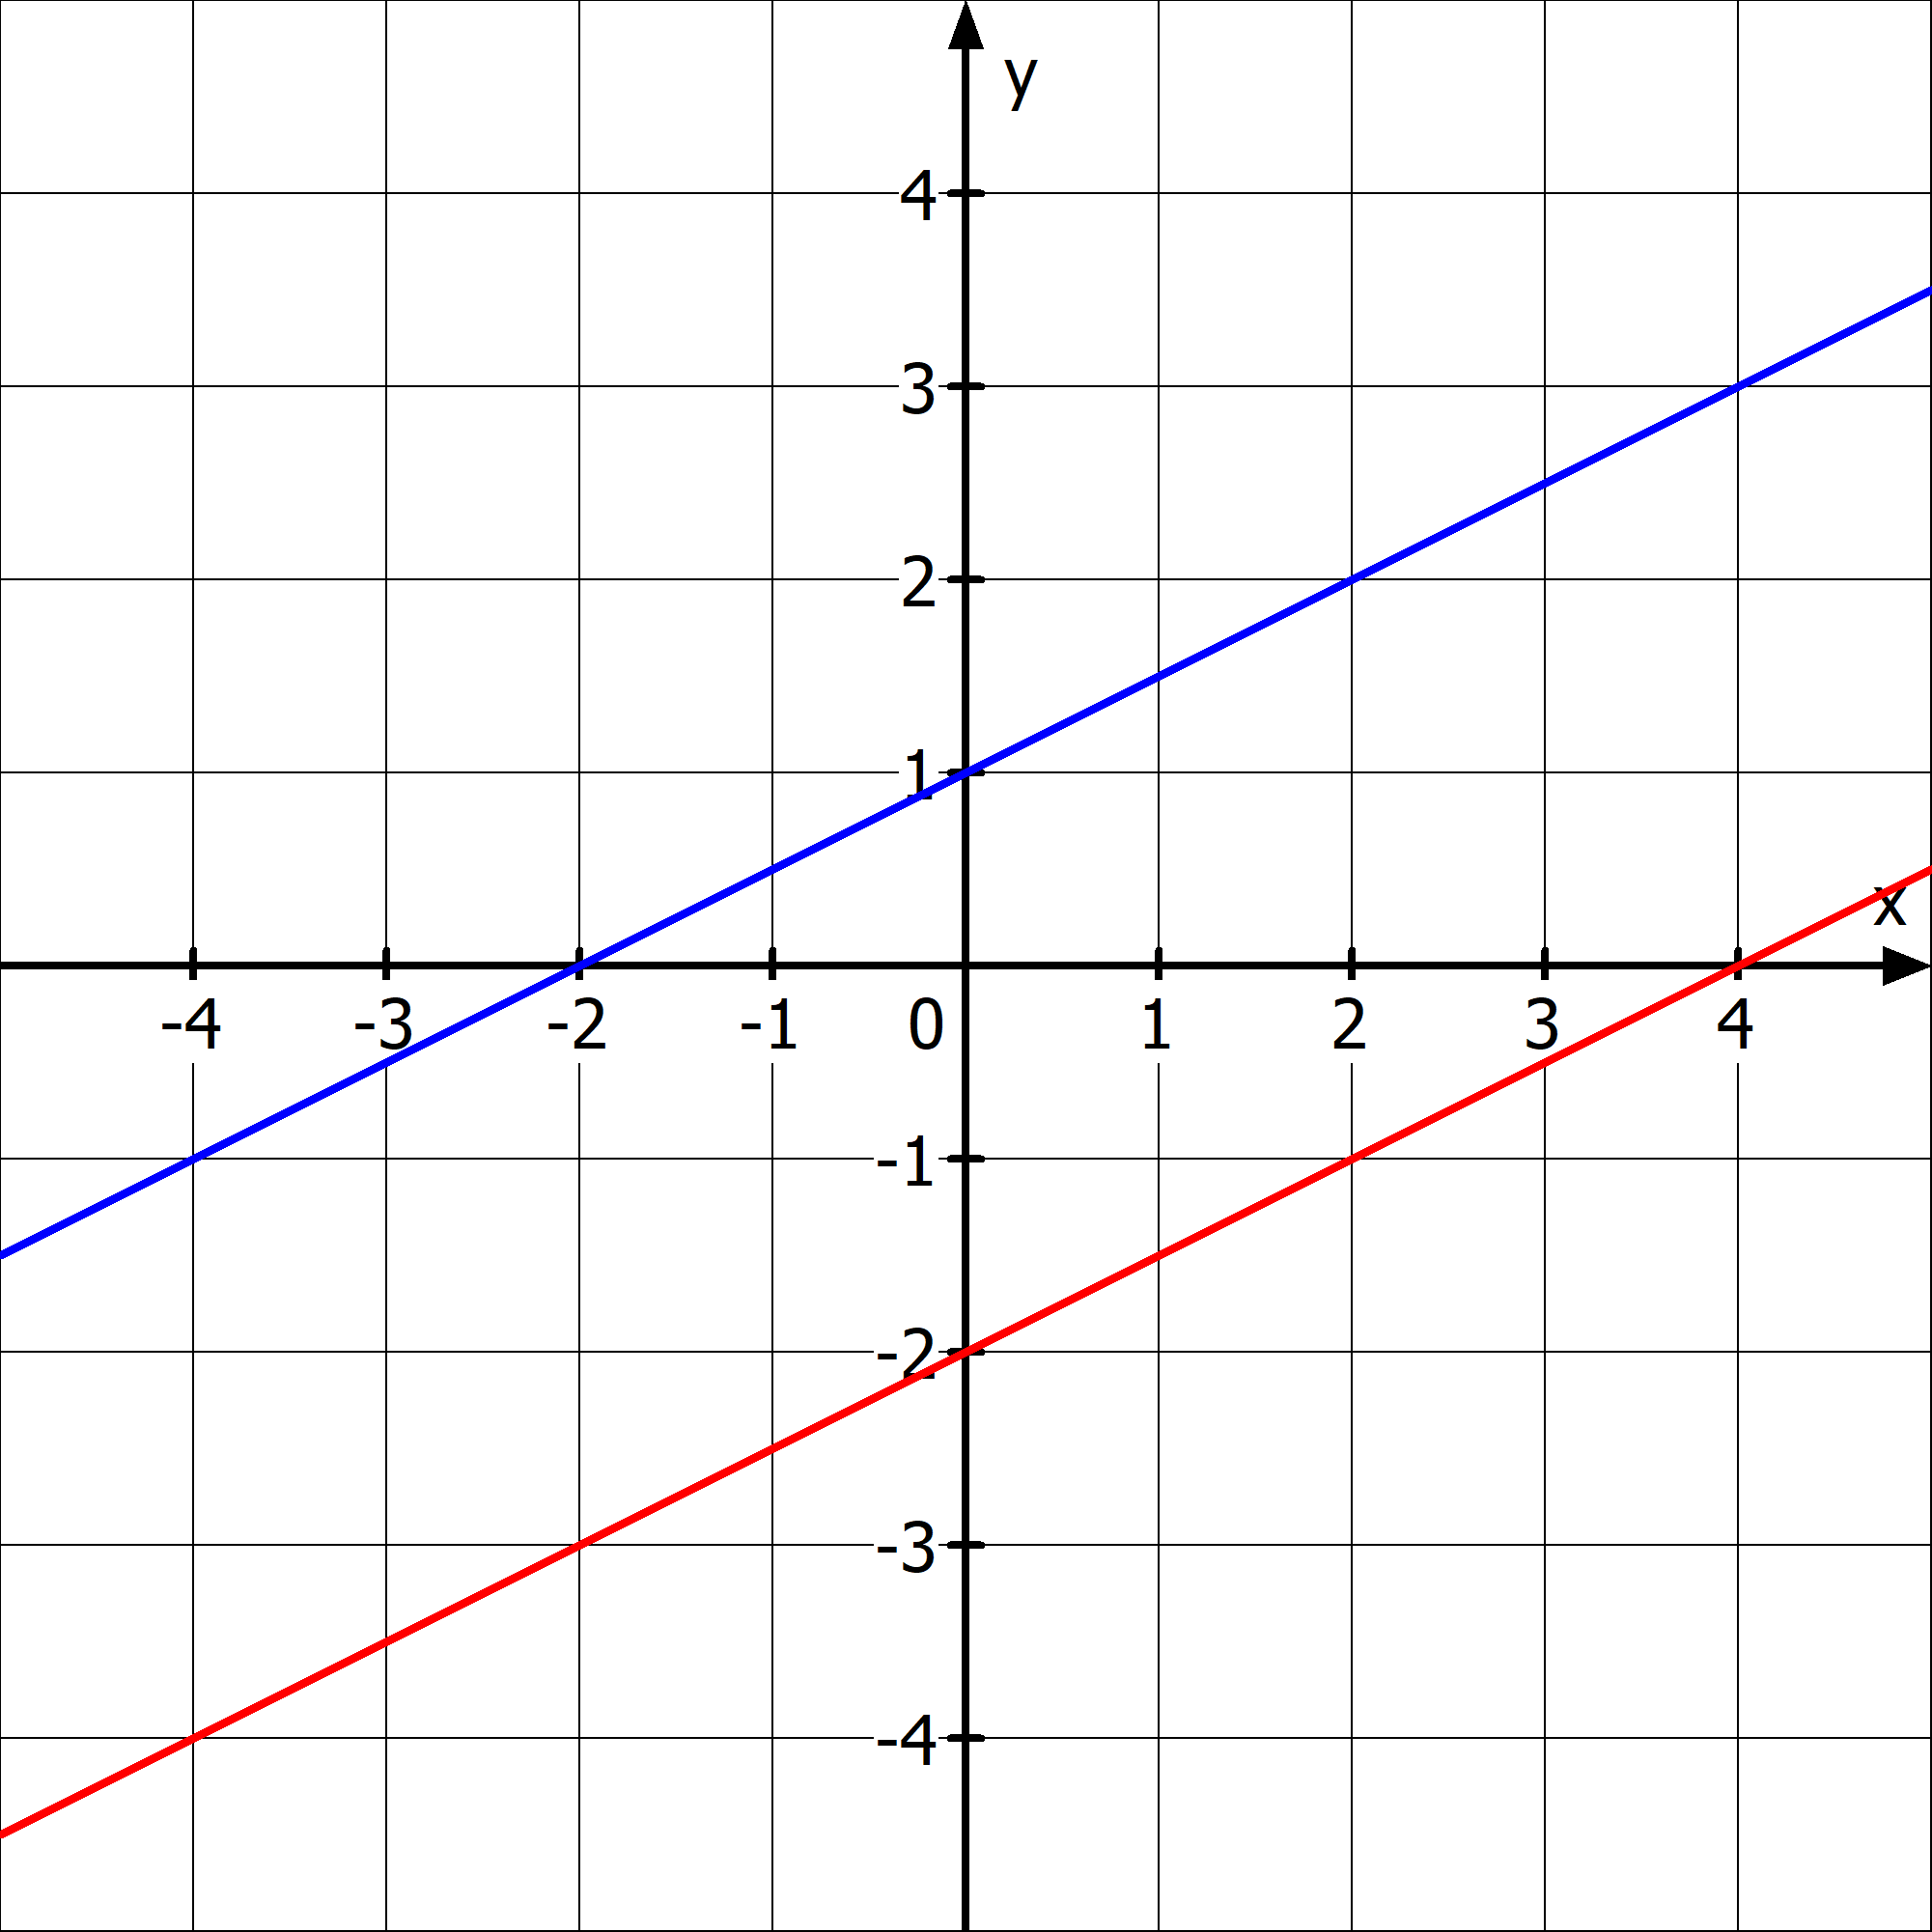
\includegraphics[width=0.45\textwidth]{\linFkt/pics/lage1.png} &
	\parbox[b]{0.46\textwidth}{\raggedright
		\begin{tcolorbox}\centering
			\textcolor{loestc}{$m_f=m_g$}
		\end{tcolorbox}
		\textcolor{loes}{Die beiden Geraden haben die gleiche Steigung. Solche Paare von Geraden nennt man parallele Geraden. Sie haben keinen Schnittpunkt, d.h. die Gleichung $f(x)=g(x)$ hat keine Lösungen. Paralle Geraden, die auch den gleichen y-Achsenabschnitt haben, nennt man identische Geraden. In diesem Fall ist jedes $x$ eine Lösung der Gleichung $f(x)=g(x)$}.\vspace{1cm}
	}
	\\
	$f_1(x)=\tfrac{1}{2}x-2\qquad g_1(x)=0,5x+1$ & \\
	\midrule
	{\Large\textcolor{loes}{keine besondere Lage}} & {\Large\textcolor{loes}{Senkrechte Geraden}}\\
	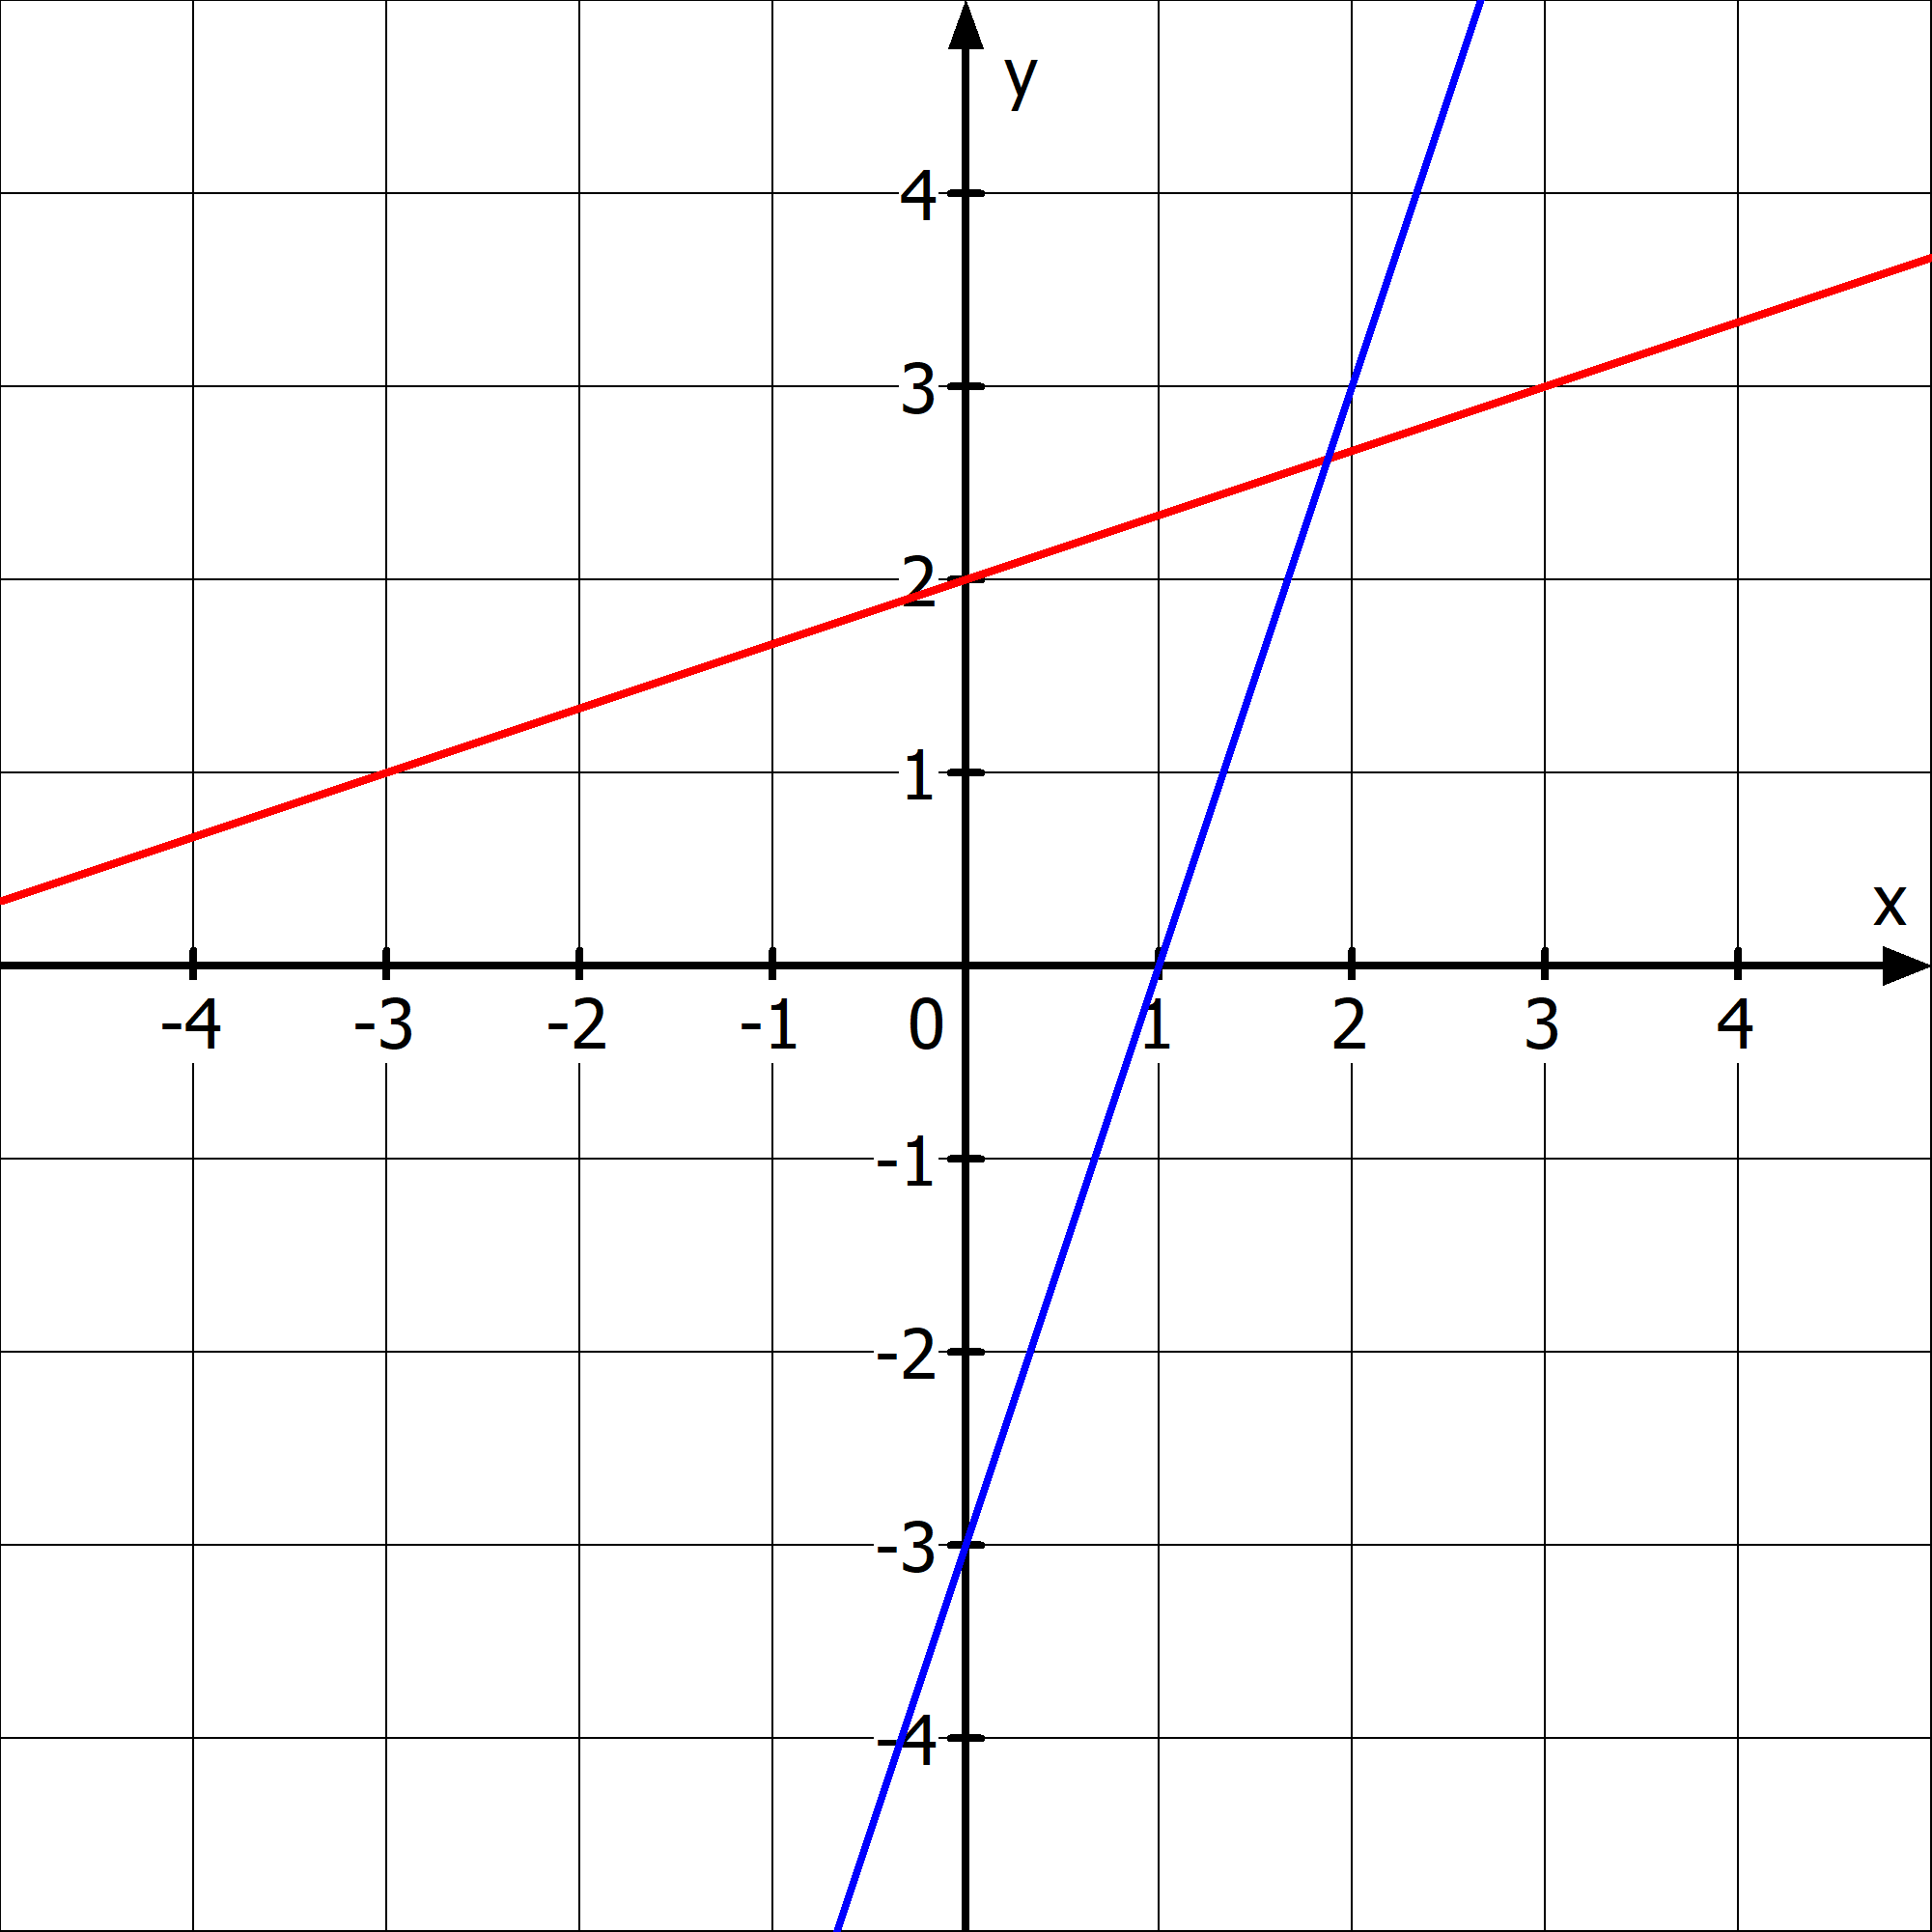
\includegraphics[width=0.5\textwidth]{\linFkt/pics/lage3.png} &
	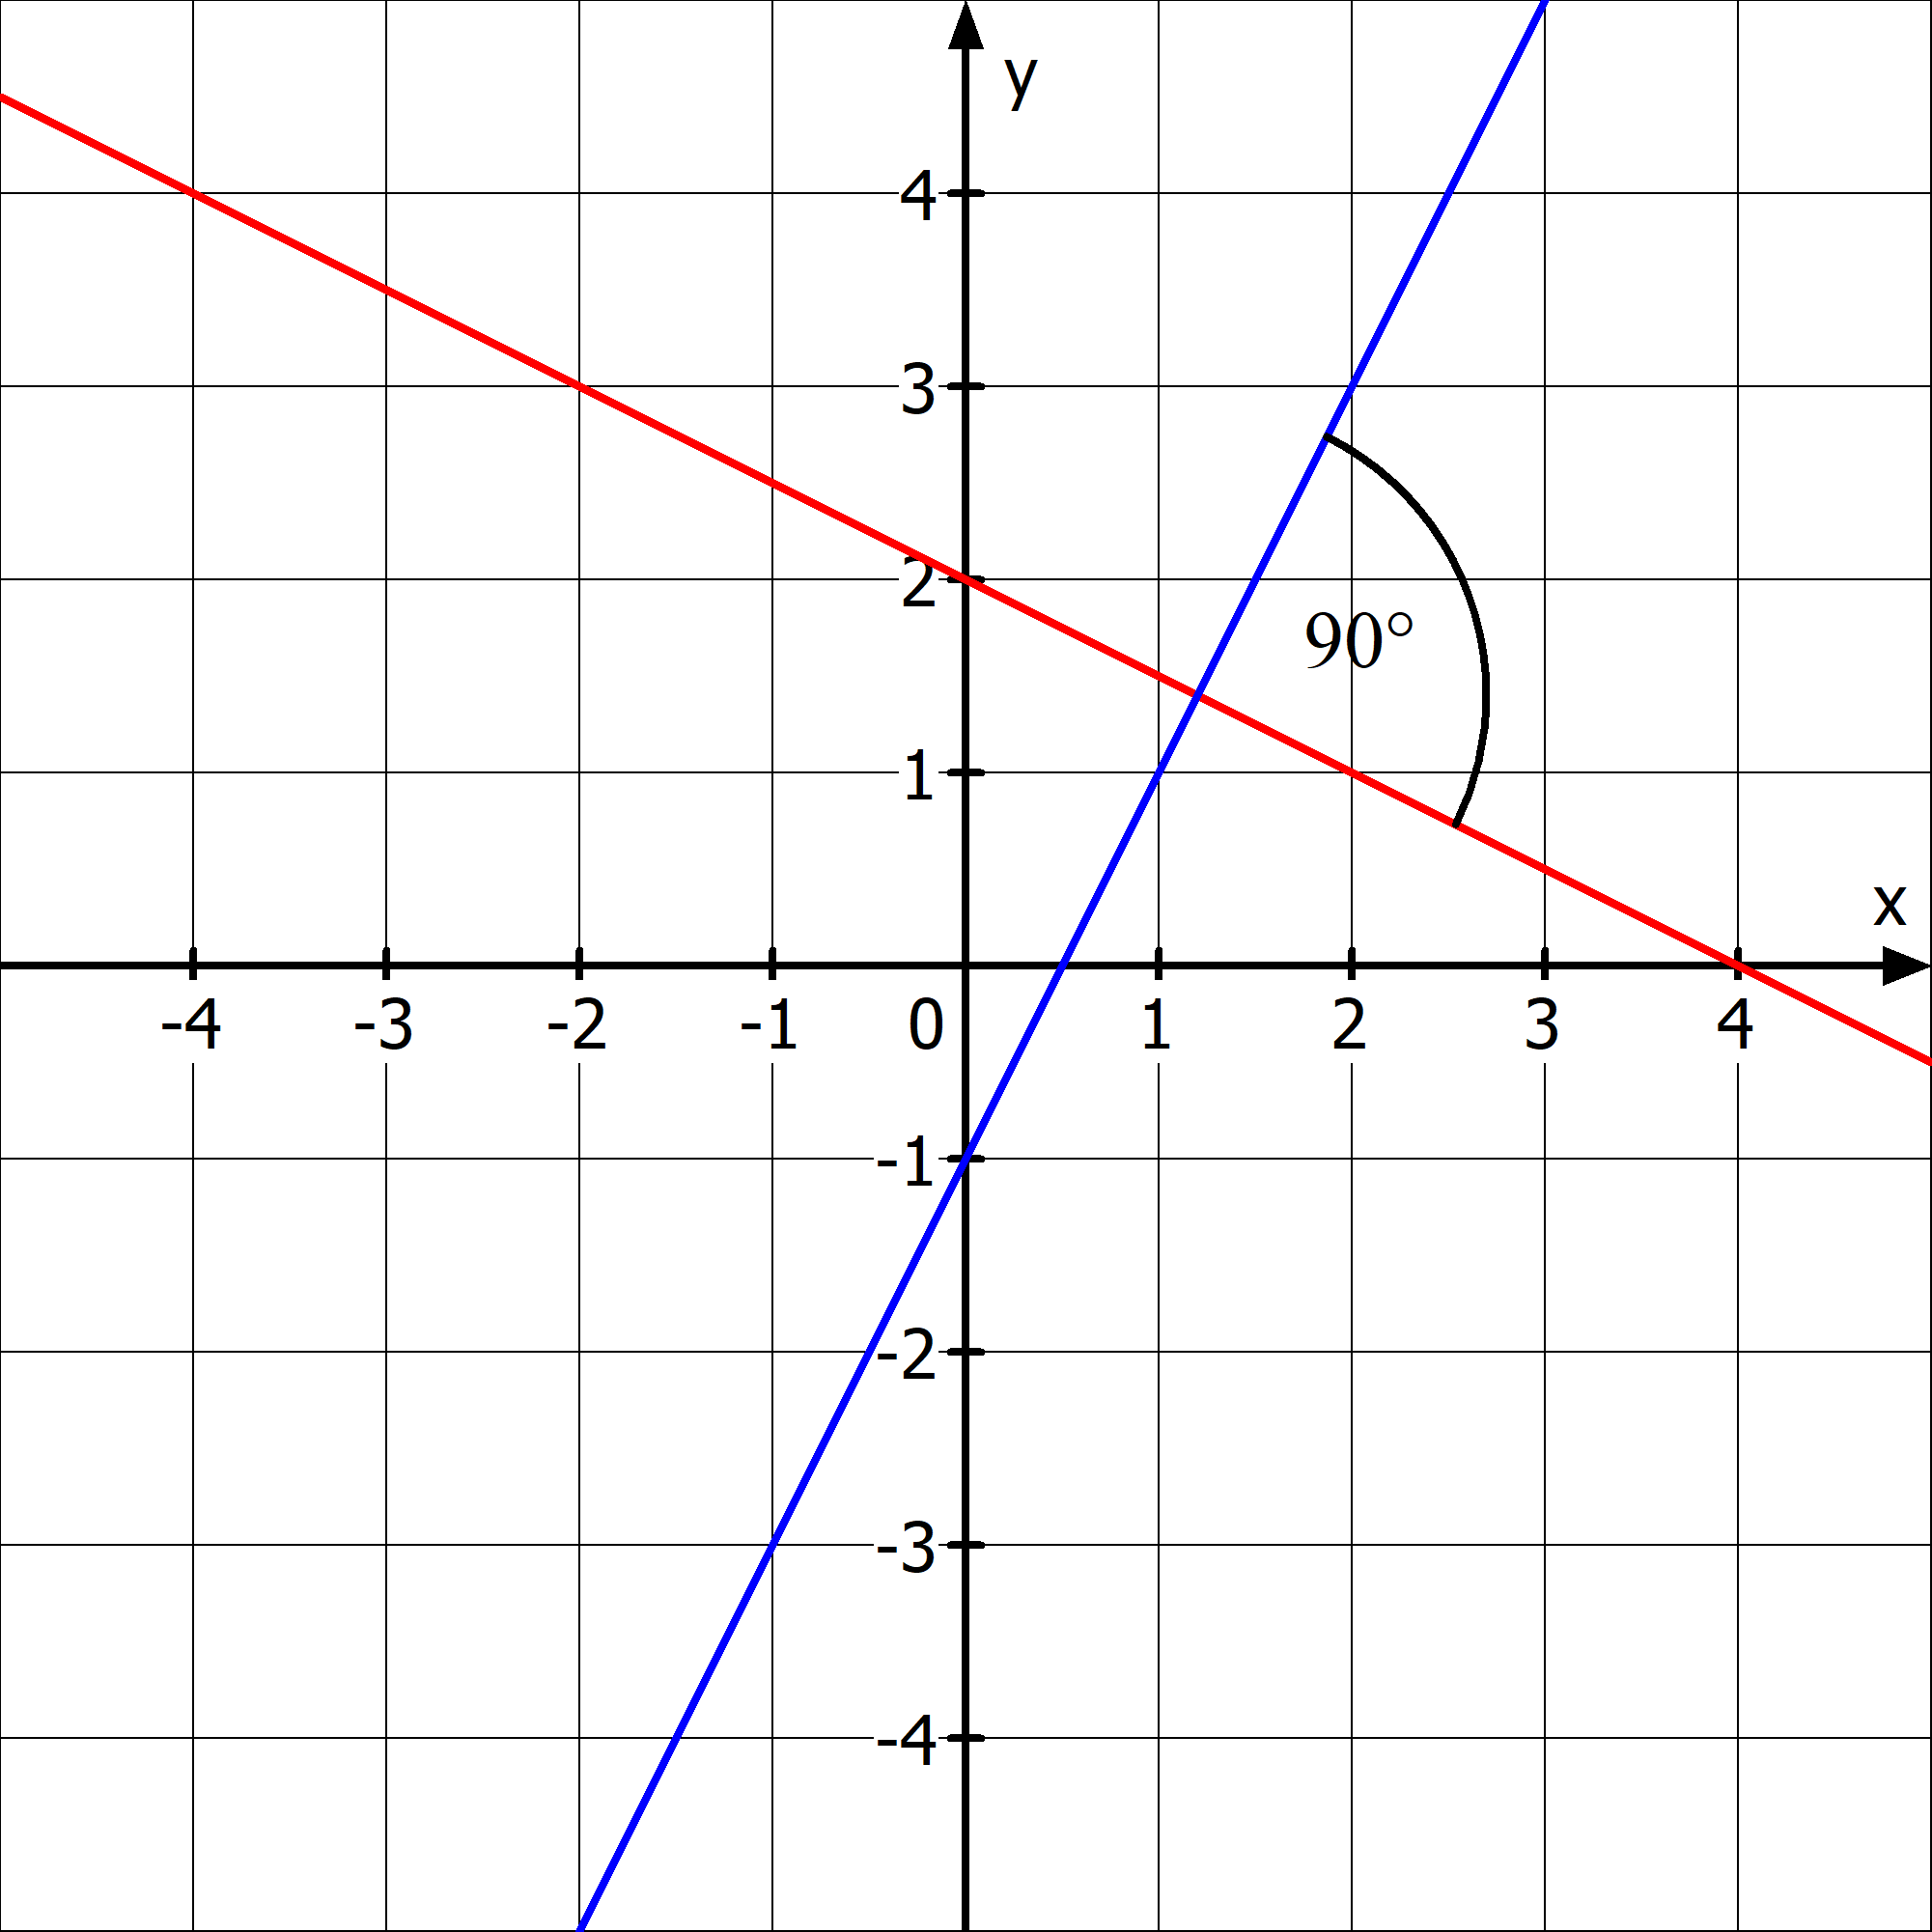
\includegraphics[width=0.5\textwidth]{\linFkt/pics/lage2.png}\\
	$f_3(x)=\tfrac{1}{3}x+2\qquad g_3(x)=3x-3$ &
	$f_2(x)=-\tfrac{1}{2}x+2\qquad g_2(x)=2x-1$\\
	\parbox[t][][t]{0.46\textwidth}{\raggedright
	\begin{tcolorbox}\centering
		\textcolor{loestc}{$m_f\neq m_g$ und $m_f\cdot m_g\neq-1$}
	\end{tcolorbox}
	\textcolor{loes}{Die beiden Geraden sind weder parallel noch orthogonal, d.h. sie haben keine besondere Lage zueinander.}.}&
	\parbox[t][][t]{0.46\textwidth}{\raggedright
	\begin{tcolorbox}\centering
		\textcolor{loestc}{$m_f\cdot m_g=-1$}
	\end{tcolorbox}
	\textcolor{loes}{Die beiden Geraden schneiden sich in einem rechten Winkel. Solche Paare von Geraden stehen orthogonal bzw. normal zueinander.
	}}\\
\end{tabular}
	\newpage
	\cohead{\Large\textbf{Schnittstellen und Schnittpunkte}}
\fakesubsection{Schnittstellen und Schnittpunkte}
Erinnerung: In der Mathematik unterscheidet man grundsätzlich zwischen Stellen und Punkten. Stellen sind x-Werte während Punkte einen x-Wert und einen y-Wert haben. Die Schnittpunkte zweier Funktionen $f(x)$ und $g(x)$ sind alle Punkte, in denen sich die Schaubilder schneiden. Um die Schnittstellen zu erhalten, muss man die Funktionen gleichsetzen:
\begin{tcolorbox}\centering
	$\textcolor{loestc}{f(x)=g(x)}$
\end{tcolorbox}
\begin{minipage}{0.49\textwidth}
	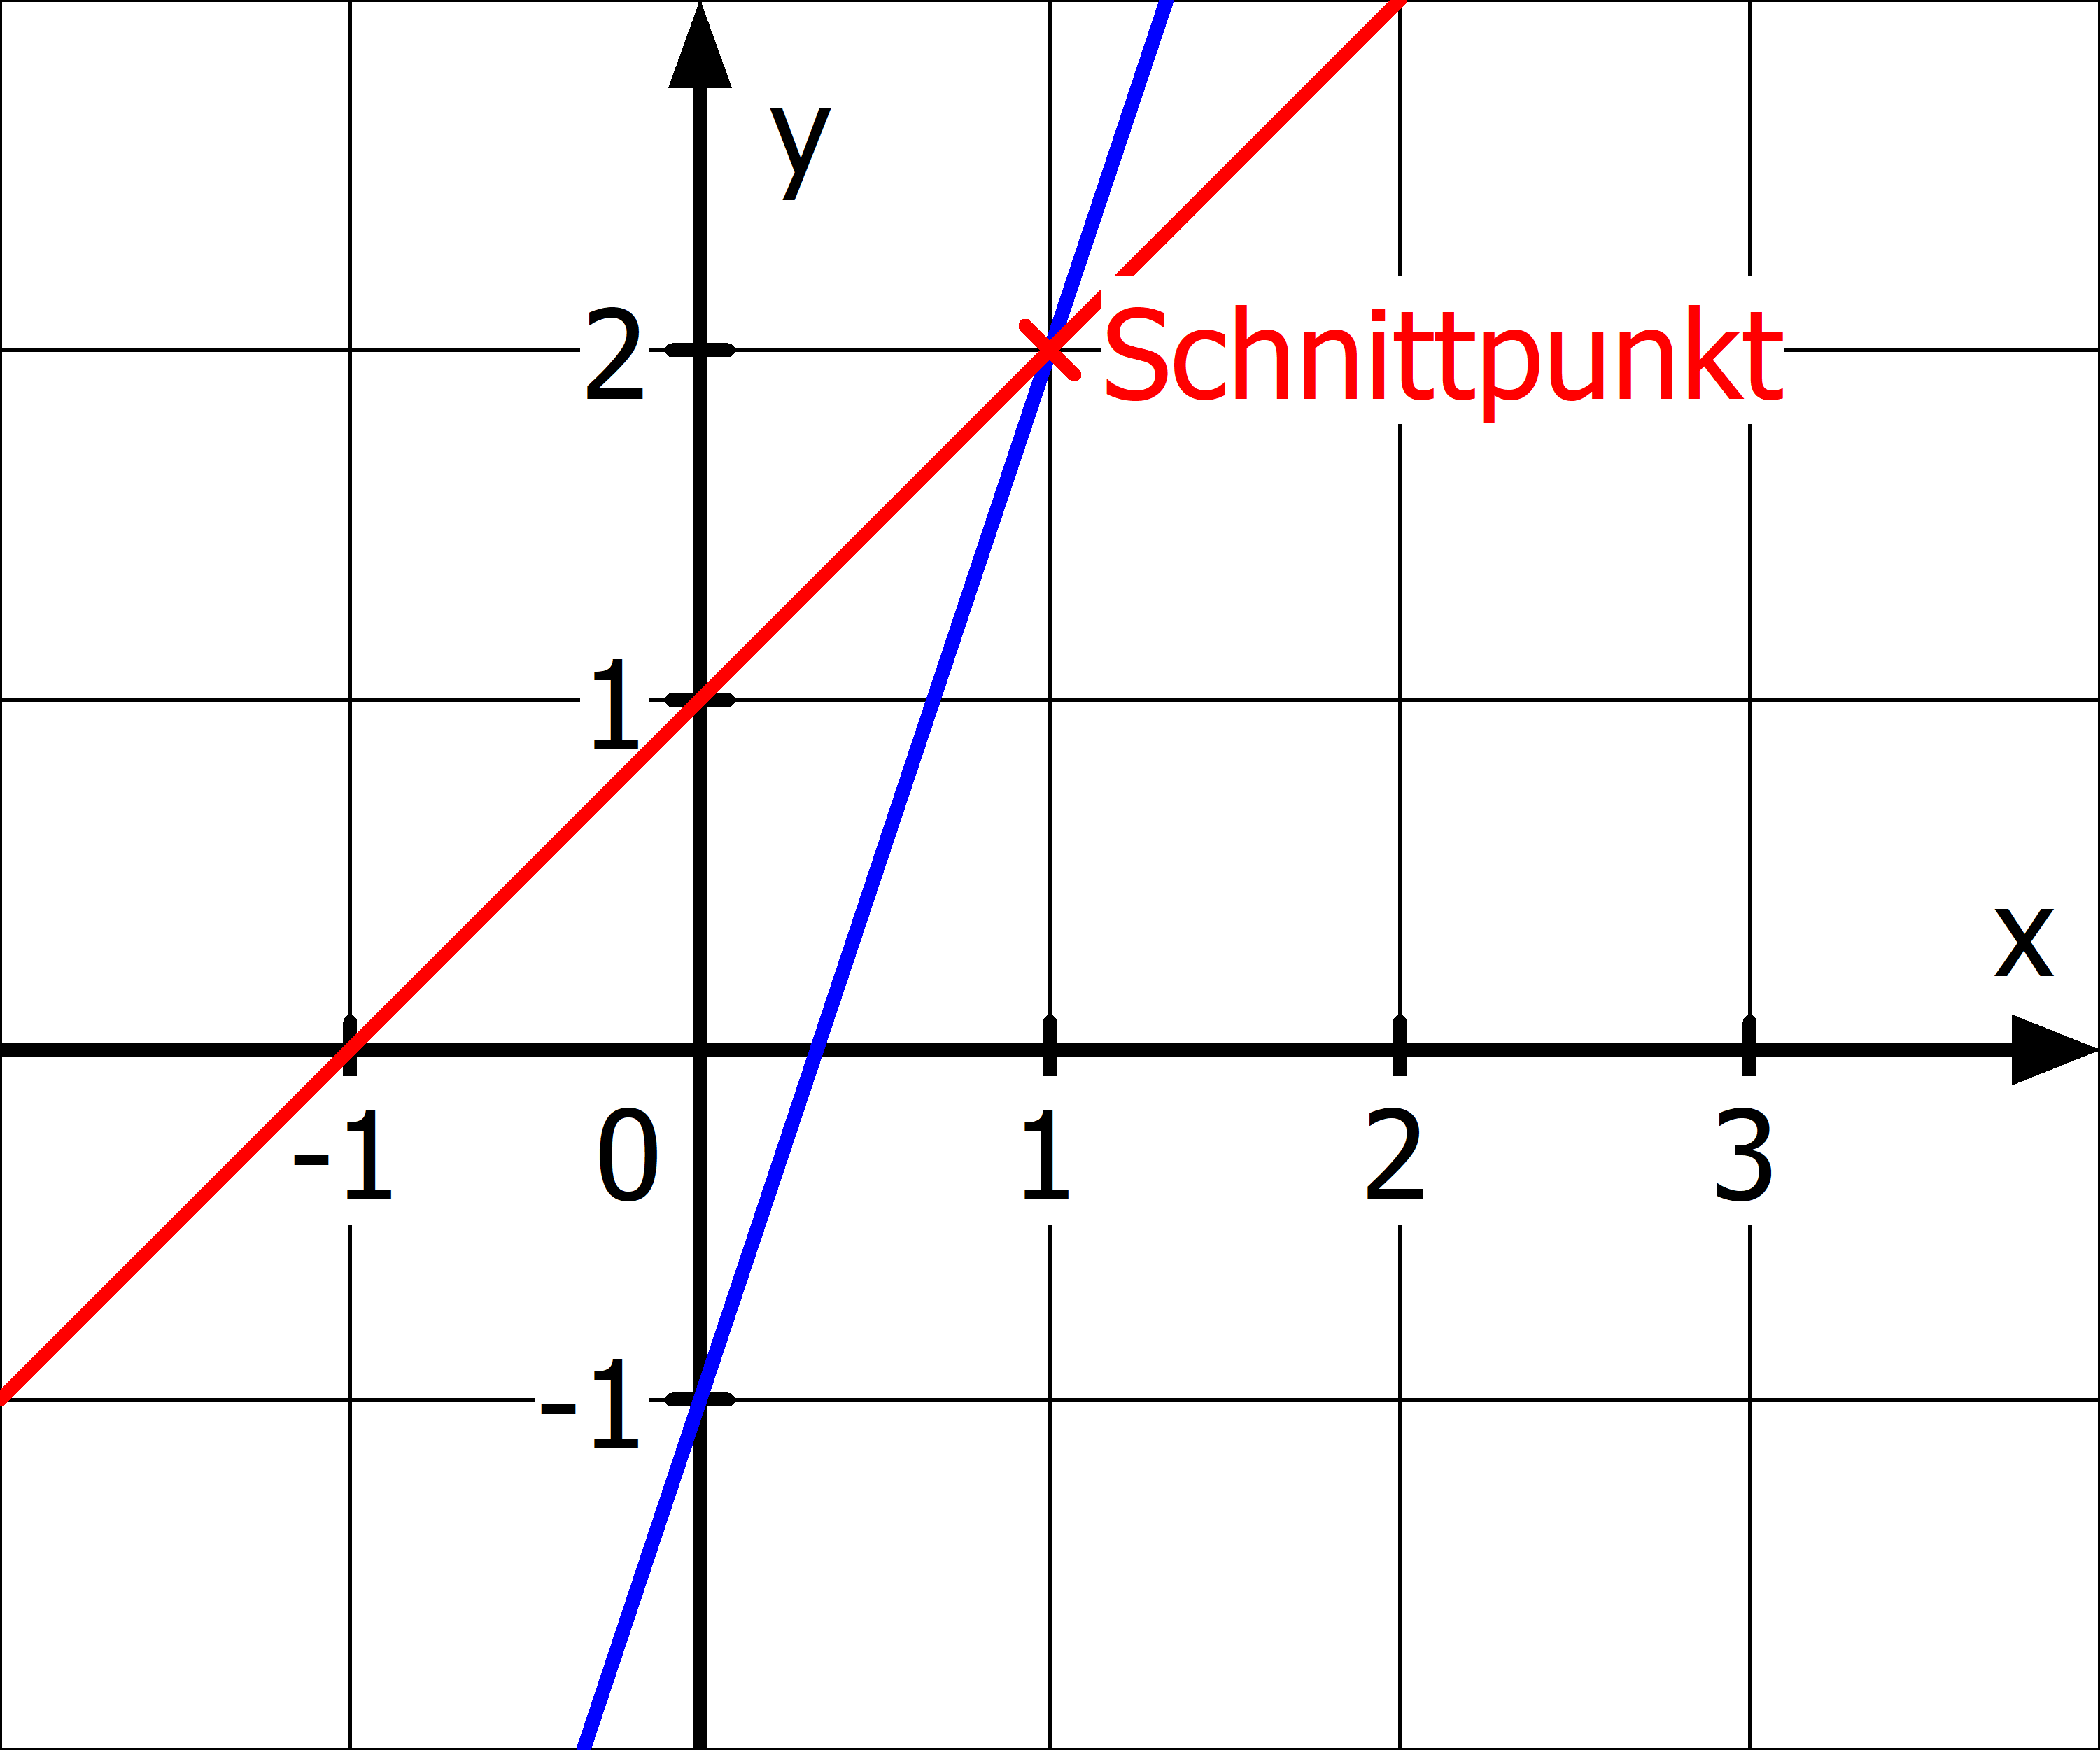
\includegraphics[width=.95\textwidth]{\linFkt/pics/schnittpunkt.png}
\end{minipage}
\begin{minipage}{0.49\textwidth}
	Im nebenstehenden Beispiel sind die Schaubilder der Funktionen $\textcolor{red}{f(x)=x+1}$ und $\textcolor{blue}{g(x)=3x-1}$ gezeichnet. Der Schnittpunkt lässt sich wie folgt berechnen:
	\begin{align*}
		\textcolor{loes}{f(x)}&\textcolor{loes}{=g(x)}\\
		\textcolor{loes}{x+1}&\textcolor{loes}{=3x-1\ \vert -3x-1}\\
		\textcolor{loes}{-2x}&\textcolor{loes}{=-2\ \vert \cdot\left(-\tfrac{1}{2}\right)}\\
		\textcolor{loes}{x}&\textcolor{loes}{=1}
	\end{align*}
\end{minipage}\smallskip\\
Die Schnittstelle ist also $\textcolor{ForestGreen}{x=1}$. Um die y-Koordinate zu erhalten, setzt man $\textcolor{ForestGreen}{x=1}$ entweder in $\textcolor{red}{f(x)}$ oder $\textcolor{blue}{g(x)}$ ein. Zur Demonstration setzen wir die Schnittstelle in beide Funktionen ein:
\begin{align*}
	\textcolor{red}{f(}\textcolor{ForestGreen}{1}\textcolor{red}{)}&=\textcolor{red}{\textcolor{ForestGreen}{1}+1}=\textcolor{YellowOrange}{2}\\
	\textcolor{blue}{g(}\textcolor{ForestGreen}{1}\textcolor{blue}{)}&=\textcolor{blue}{3\cdot \textcolor{ForestGreen}{1}-1}=\textcolor{YellowOrange}{2}
\end{align*}
Der Schnittpunkt liegt also bei $P\left(\textcolor{ForestGreen}{1}\lvert\textcolor{YellowOrange}{2}\right)$.
\begin{Exercise}[title={Bestimme jeweils den Schnittpunkt}, label=schnittpunktA1]\\
	\begin{minipage}{0.5\textwidth}
		\begin{enumerate}[label=\alph*)]
			\item $f_1(x)=x-1$ und $g_1(x)=-x+3$
			\item $f_2(x)=-2x+4$ und $g_2(x)=0,5x-1$
			\item $f_3(x)=\frac{3}{2}x+\frac{1}{2}$ und $g_3(x)=4x$
		\end{enumerate}
	\end{minipage}
	\begin{minipage}{0.5\textwidth}
		\begin{enumerate}[label=\alph*)]
			\setcounter{enumi}{3}
			\item $f_4(x)=\frac{4}{5}x+\frac{2}{5}$ und $g_4(x)=-\frac{2}{5}x$
			\item $f_5(x)=-\frac{2}{3}x-15$ und $g_5(x)=3x-\frac{5}{4}$
			\item $f_6(x)=-\frac{5}{8}x$ und $g_6(x)=-\frac{3}{2}x+\frac{1}{2}$
		\end{enumerate}
	\end{minipage}
\end{Exercise}\vspace{.5cm}
\begin{Answer}[ref=schnittpunktA1]\\
	\begin{minipage}{0.5\textwidth}
		\begin{enumerate}[label=\alph*)]
			\item $P_1\left(2\vert 1\right)$
			\item $P_2\left(2\vert 0\right)$
			\item $P_3\left(\frac{1}{5}\vert \frac{4}{5}\right)$
		\end{enumerate}
	\end{minipage}
	\begin{minipage}{0.5\textwidth}
		\begin{enumerate}[label=\alph*)]
			\setcounter{enumi}{3}
			\item $P_4\left(-\frac{1}{3}\vert \frac{2}{15}\right)$
			\item $P_5\left(-\frac{15}{4}\vert -\frac{25}{2}\right)$
			\item $P_6\left(\frac{4}{7}\vert -\frac{5}{14}\right)$
		\end{enumerate}
	\end{minipage}
\end{Answer}
	\newpage
%%	\cohead{\Large\textbf{Lösungen}}
%%	\fakesubsection{Lösungen}
%%	\shipoutAnswer
%%	\newpage
%	%%%%%%%%%%%%%%%%%%%%%%%%%%%%%%%%%%%%%%%%%%%%%%%%%%%%%%%%%%%%%%%%%%%%%%%%%
	\fakesection{Quadratische Funktionen}
	\cohead{\Large\textbf{Scheitelform}}
\fakesubsection{Scheitelform}
\begin{minipage}{0.49\textwidth}\centering
	\textcolor{loes}{Das Schaubild der Funktion}\newline
	\textcolor{loes}{$f(x)=x^2$}\newline
	\textcolor{loes}{bezeichnet man als Normalparabel.}
\end{minipage}
\begin{minipage}{0.49\textwidth}
	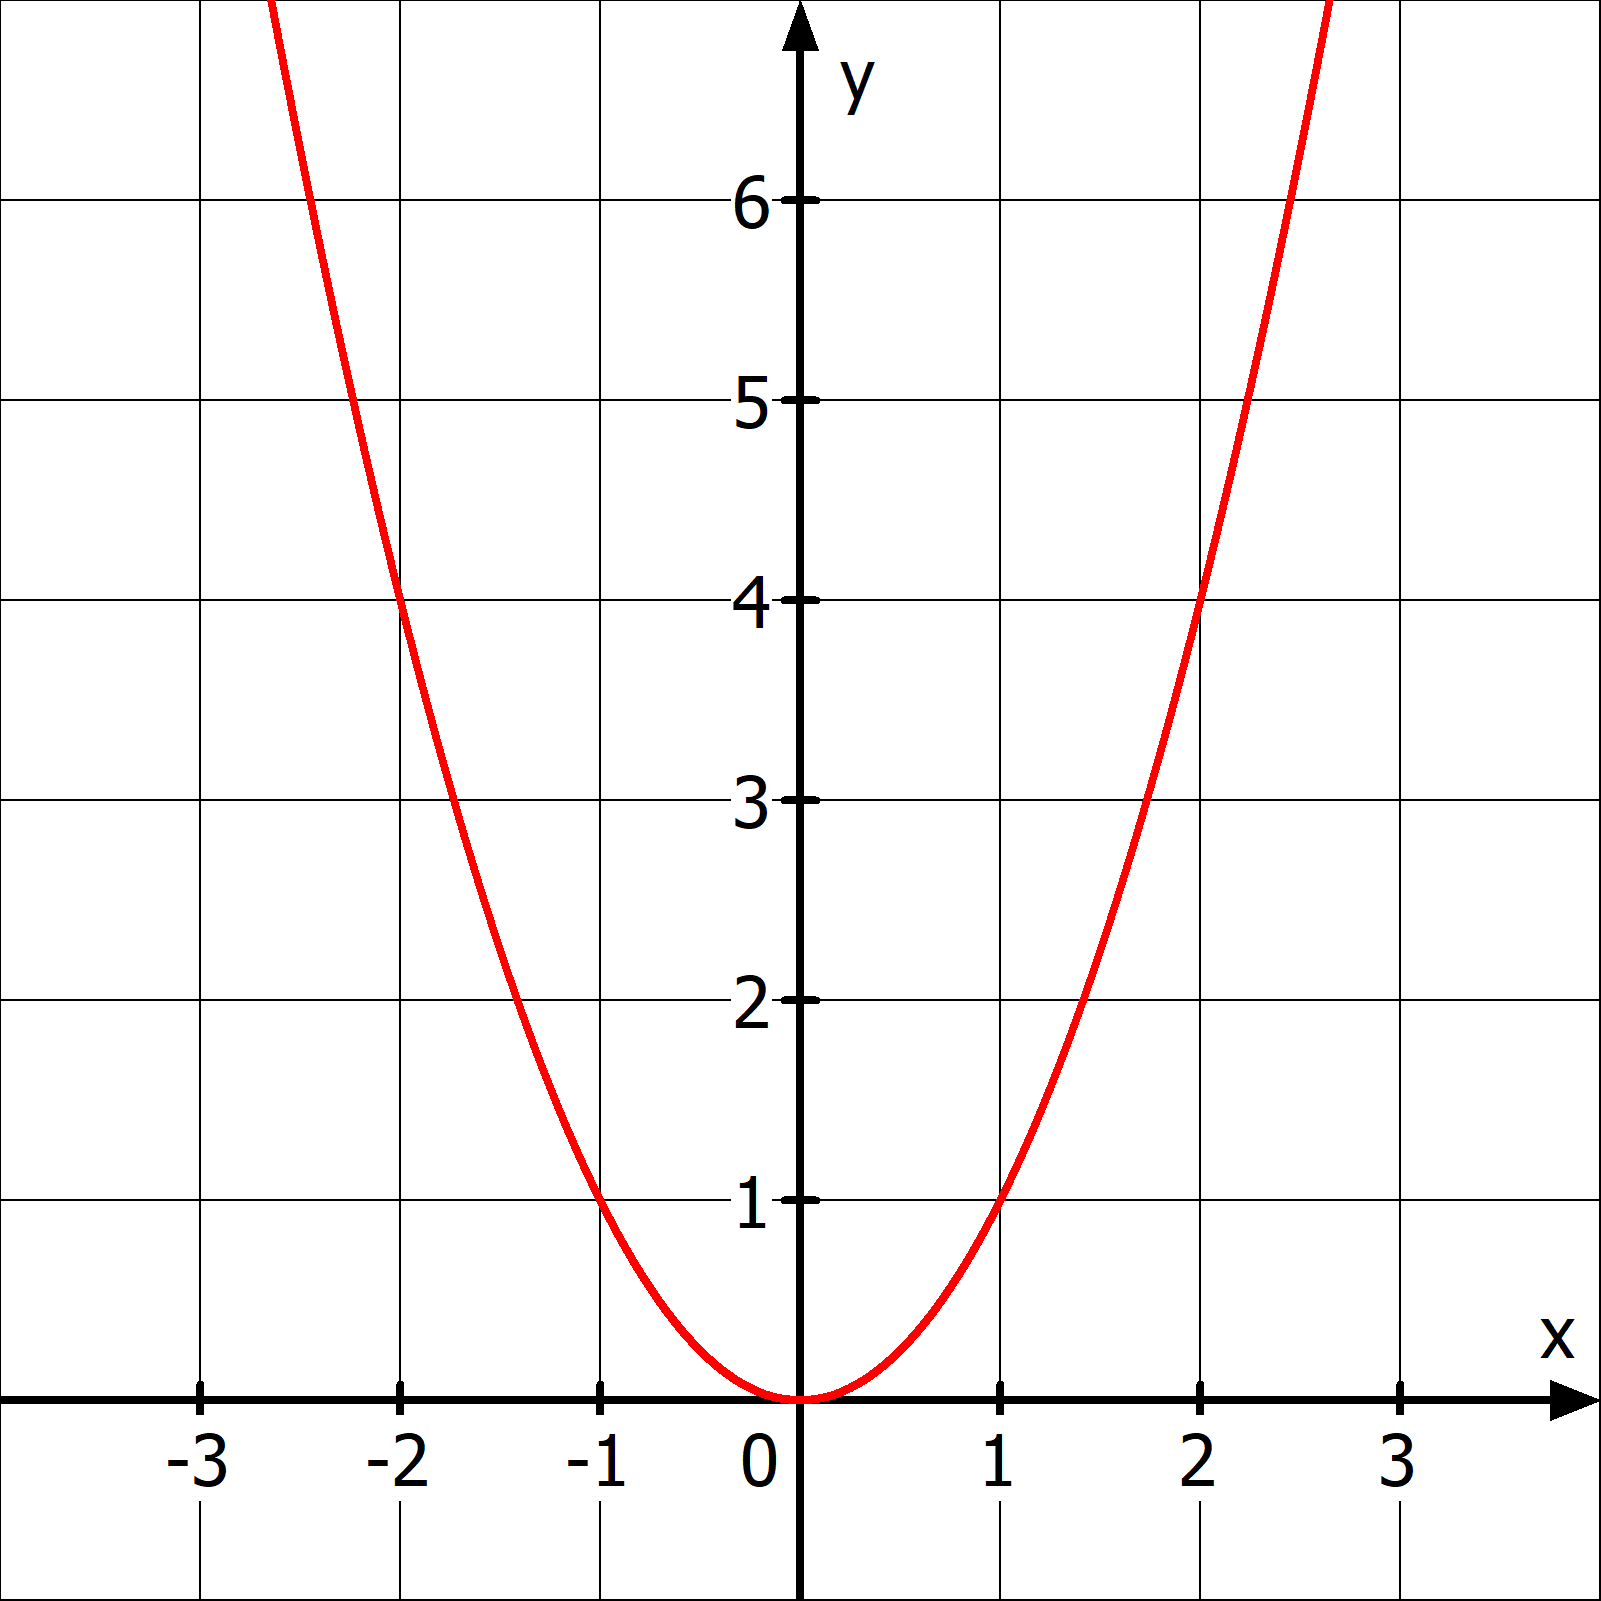
\includegraphics[width=.95\textwidth]{\quadFkt/pics/normalparabel.png}
\end{minipage}\\
\textbf{Verschieben in y-Richtung}
\begin{tcolorbox}\centering
	$\textcolor{loestc}{f(x)=x^2+y_S}$
\end{tcolorbox}
\textcolor{loes}{Für $y_S>0$ wird die Parabel nach oben verschoben, für $y_S<0$ wird die Parabel nach unten verschoben.}\\
\textbf{Verschieben in x-Richtung}
\begin{tcolorbox}\centering
	$\textcolor{loestc}{f(x)=\left(x-x_S\right)^2}$
\end{tcolorbox}
\textcolor{loes}{Für $x_S>0$ wird die Parabel nach rechts verschoben, für $x_S<0$ wird die Parabel nach links verschoben.}\\
\textbf{Strecken und Stauchen}
\begin{tcolorbox}\centering
	$\textcolor{loestc}{f(x)=a\cdot x^2}$
\end{tcolorbox}
\textcolor{loes}{Für $a>1$ wird die Parabel gestreckt, sie erscheint dann schmäler.}\\
\textcolor{loes}{Für $0<a<1$ wird die Parabel gestaucht, sie erscheint dann breiter.}\\
\textcolor{loes}{Für negative $a$ wird die Parabel zusätzlich nach unten geklappt.}\\
\textbf{Scheitelform}
\begin{tcolorbox}\centering
	$\textcolor{loestc}{f(x)=a\cdot \left(x-x_S\right)^2+y_S}$
\end{tcolorbox}
\textcolor{loes}{Man kann die Parabel gleichzeitig in x-Richtung und y-Richtung verschieben sowie strecken oder stauchen. Man erhält so die Scheitelform. Liegt die Funktionsgleichung einer Parabel in der Scheitelform vor, so kann man den Scheitel $S\left(x_S\vert y_S \right)$ direkt ablesen.}\newpage
%%%%%%%%%%%%%%%%%%%%%%%%%%%%%%%%%%%%%%%%%
\cohead{\Large\textbf{Verschieben in y-Richtung}}
\begin{tabular}{cc}
	\begin{minipage}{0.47\textwidth}
		\centering\Large\textcolor{loes}{Die Normalparabel wird um 2 Einheiten nach unten verschoben.\newline\newline$f(x)=x^2-2$\newline\newline Der Scheitel liegt bei $S\left(0\vert -2\right) $}
	\end{minipage}
	&
	\begin{minipage}{0.47\textwidth}
		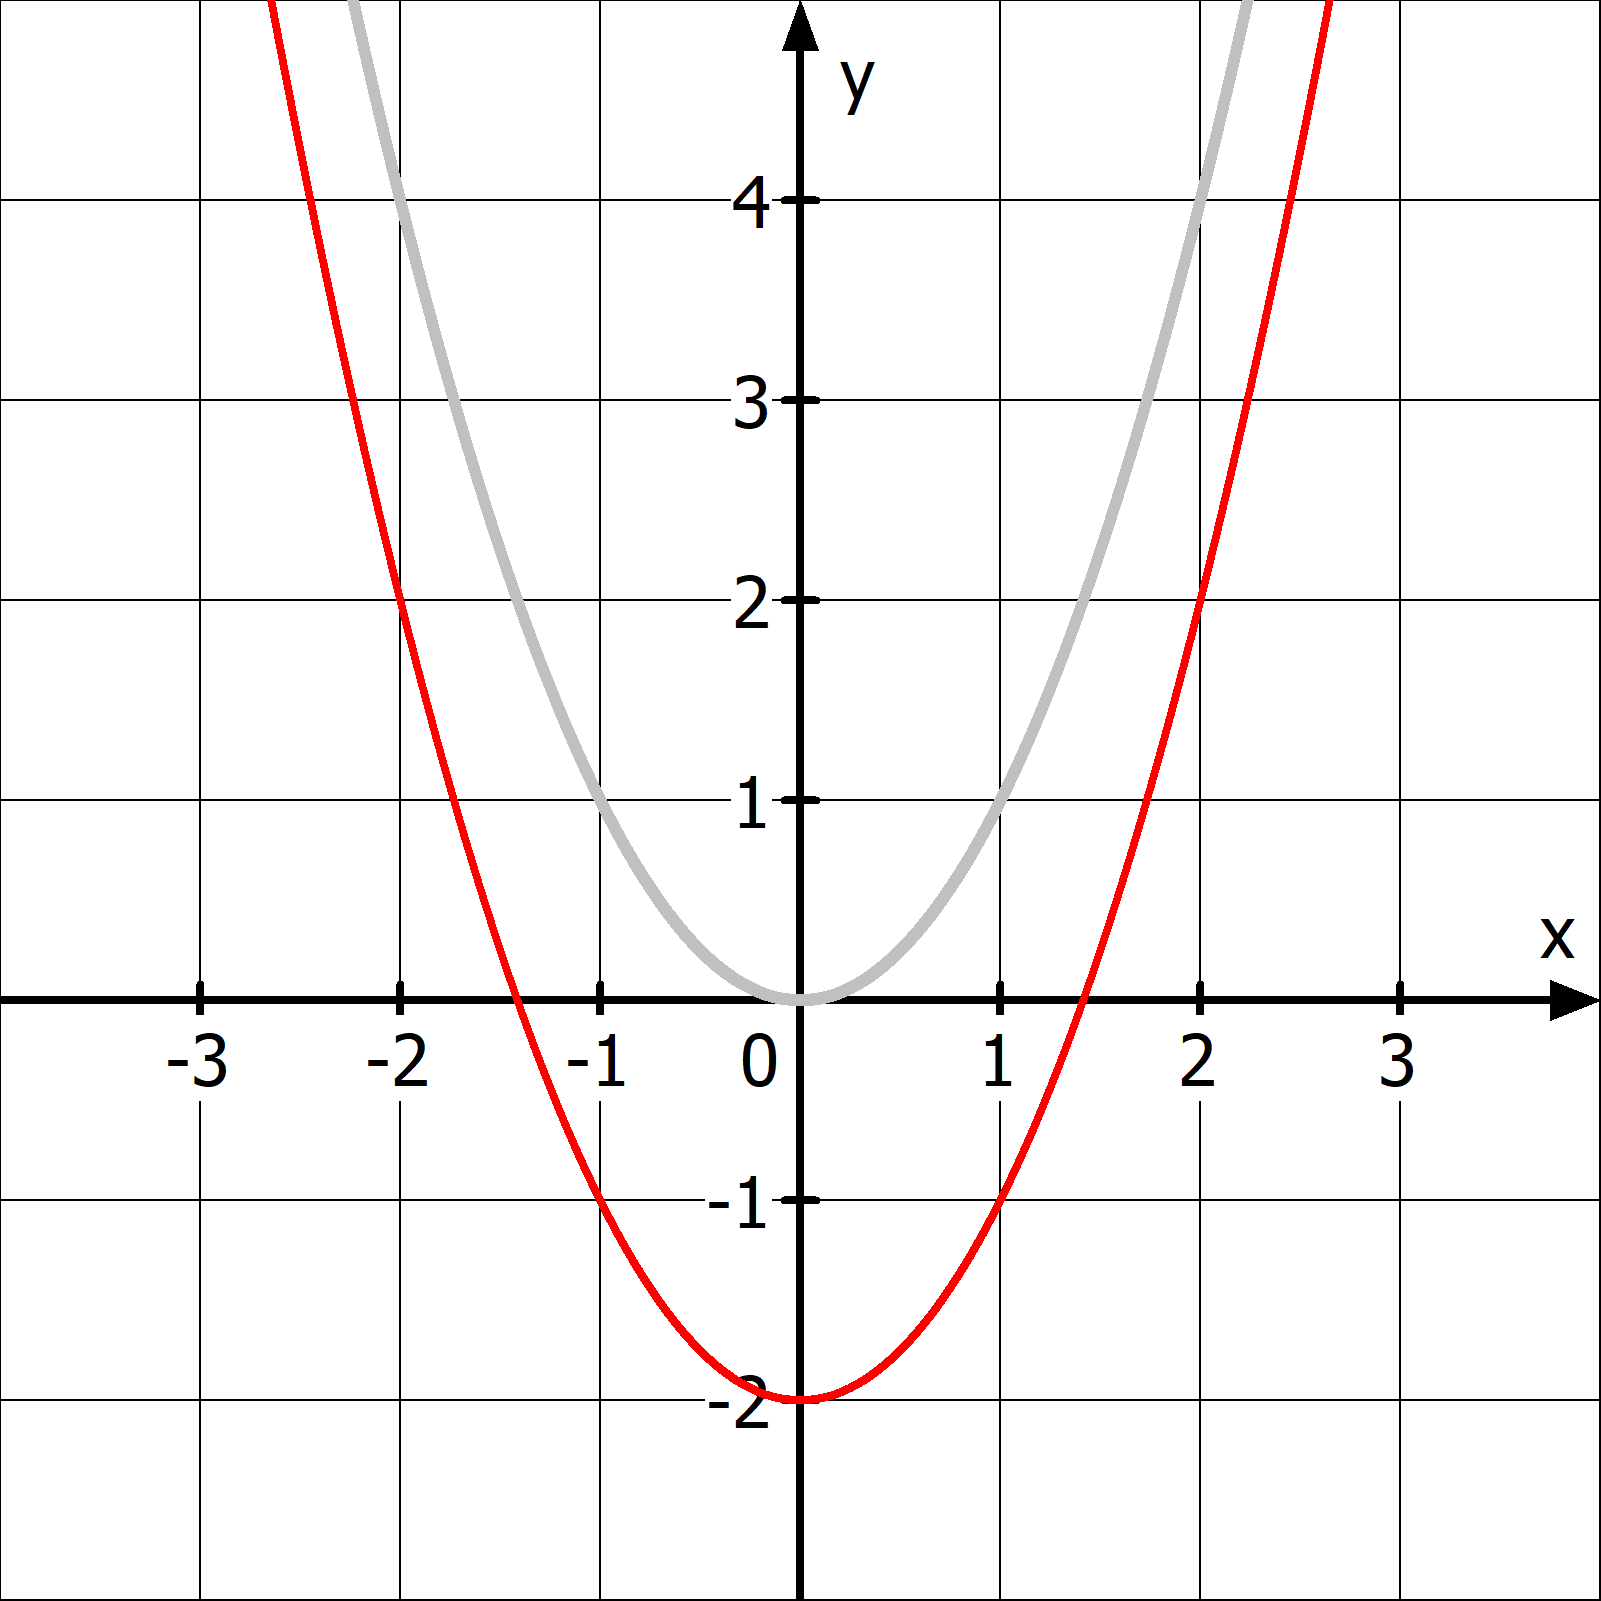
\includegraphics[width=.95\textwidth]{\quadFkt/pics/verschiebenY1.png}
	\end{minipage} \\
	\midrule
	\begin{minipage}{0.47\textwidth}
		\centering\Large Die Normalparabel wird um 3 Einheiten nach oben verschoben.\newline\newline\textcolor{loes}{$f(x)=x^2+3$\newline\newline Der Scheitel liegt bei $S\left(0\vert 3\right) $}
	\end{minipage}
	&
	\begin{minipage}{0.47\textwidth}
		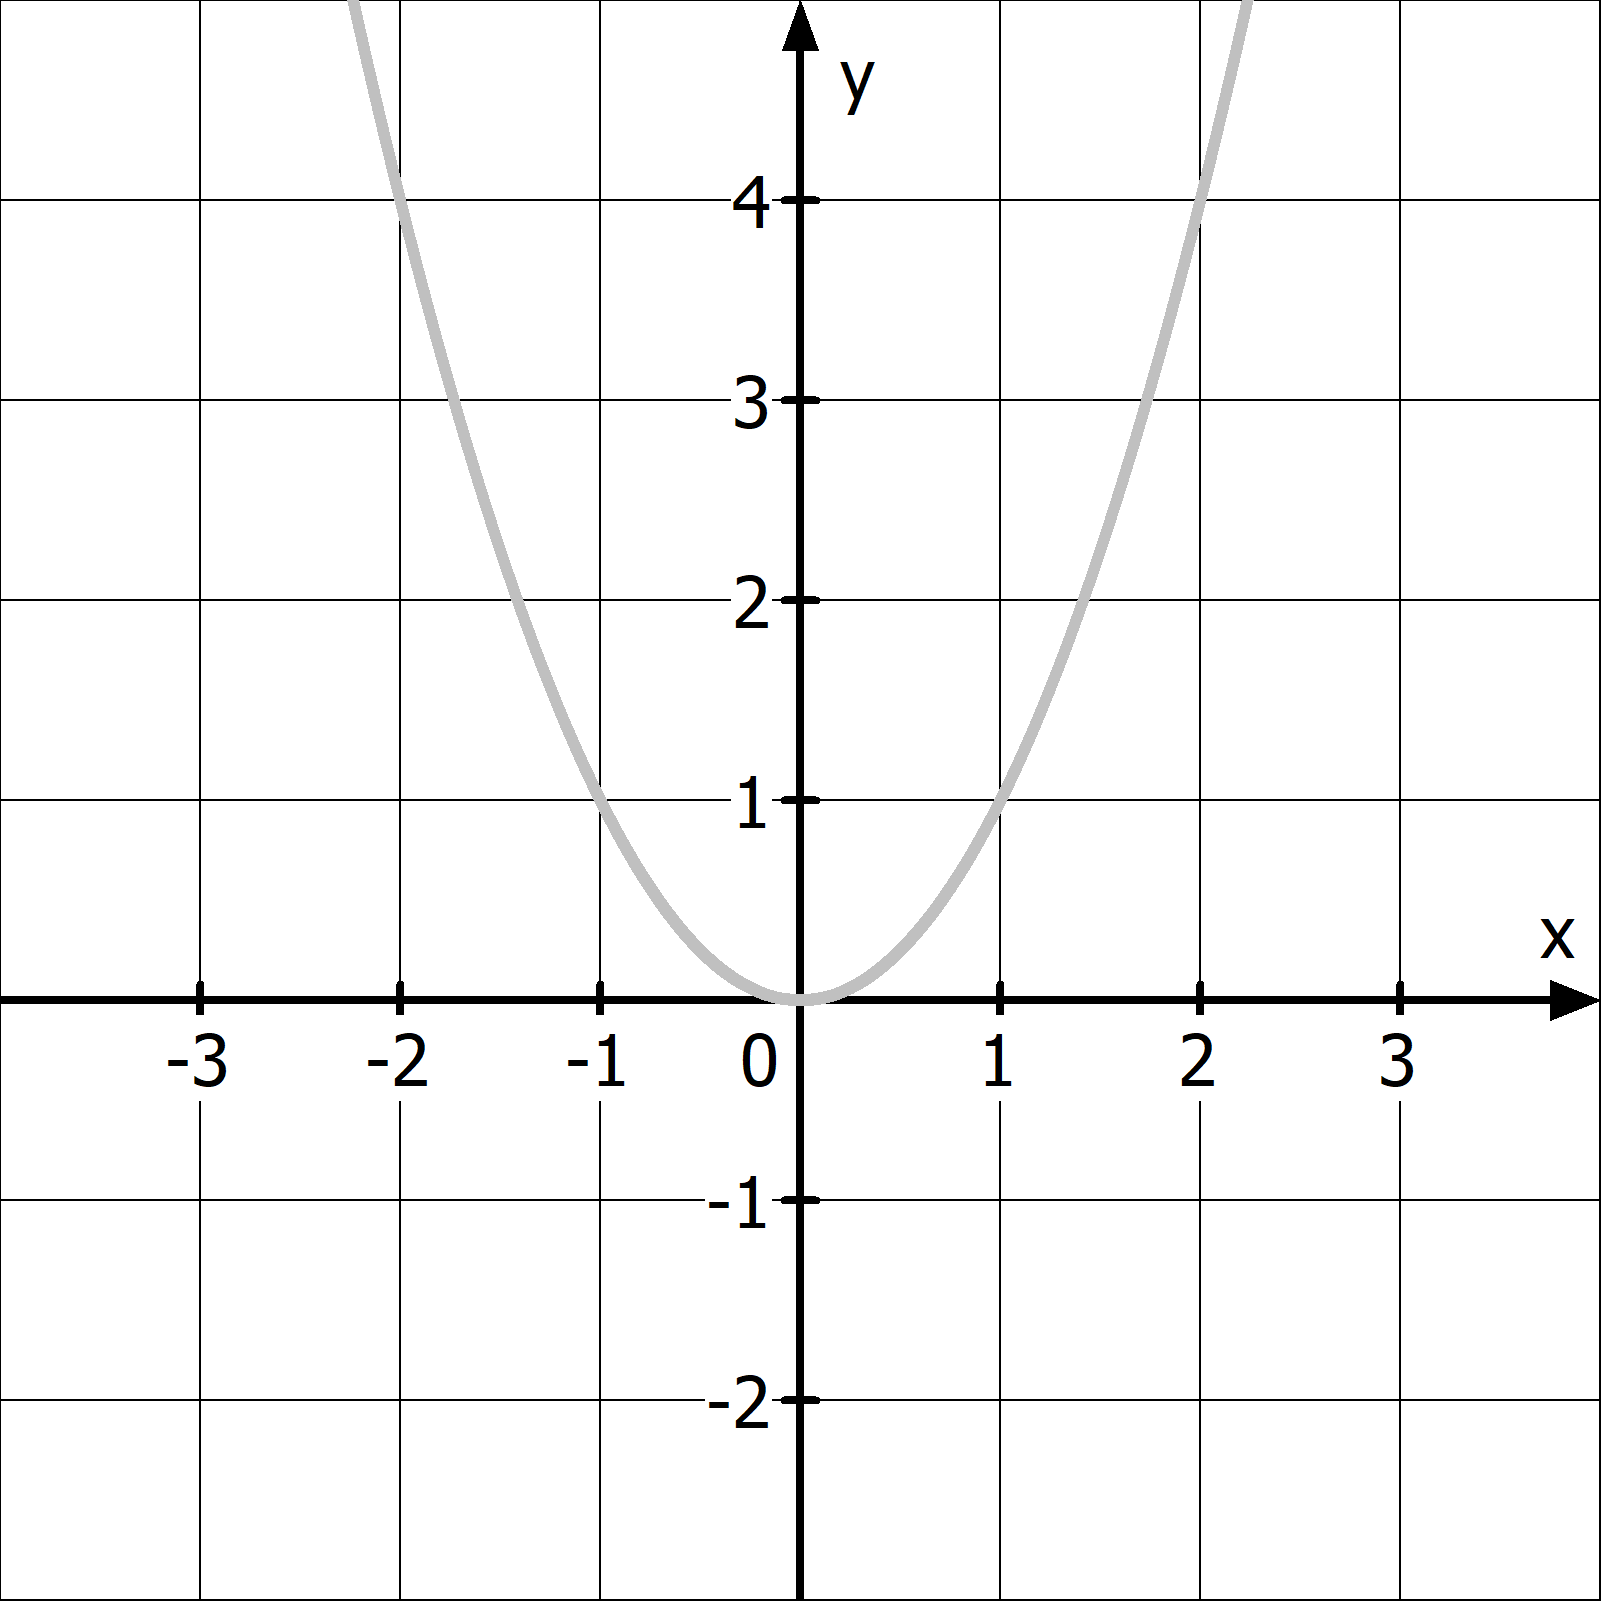
\includegraphics[width=.95\textwidth]{\quadFkt/pics/verschieben_empty.png}
	\end{minipage} \\
	\midrule
	\begin{minipage}{0.47\textwidth}
		\centering\Large\textcolor{loes}{Die Normalparabel wird um 2 Einheiten nach unten verschoben.}\newline\newline$f(x)=x^2-2$\newline\newline Der Scheitel liegt bei $S\left(0\vert -2\right) $
	\end{minipage}
	&
	\begin{minipage}{0.47\textwidth}
		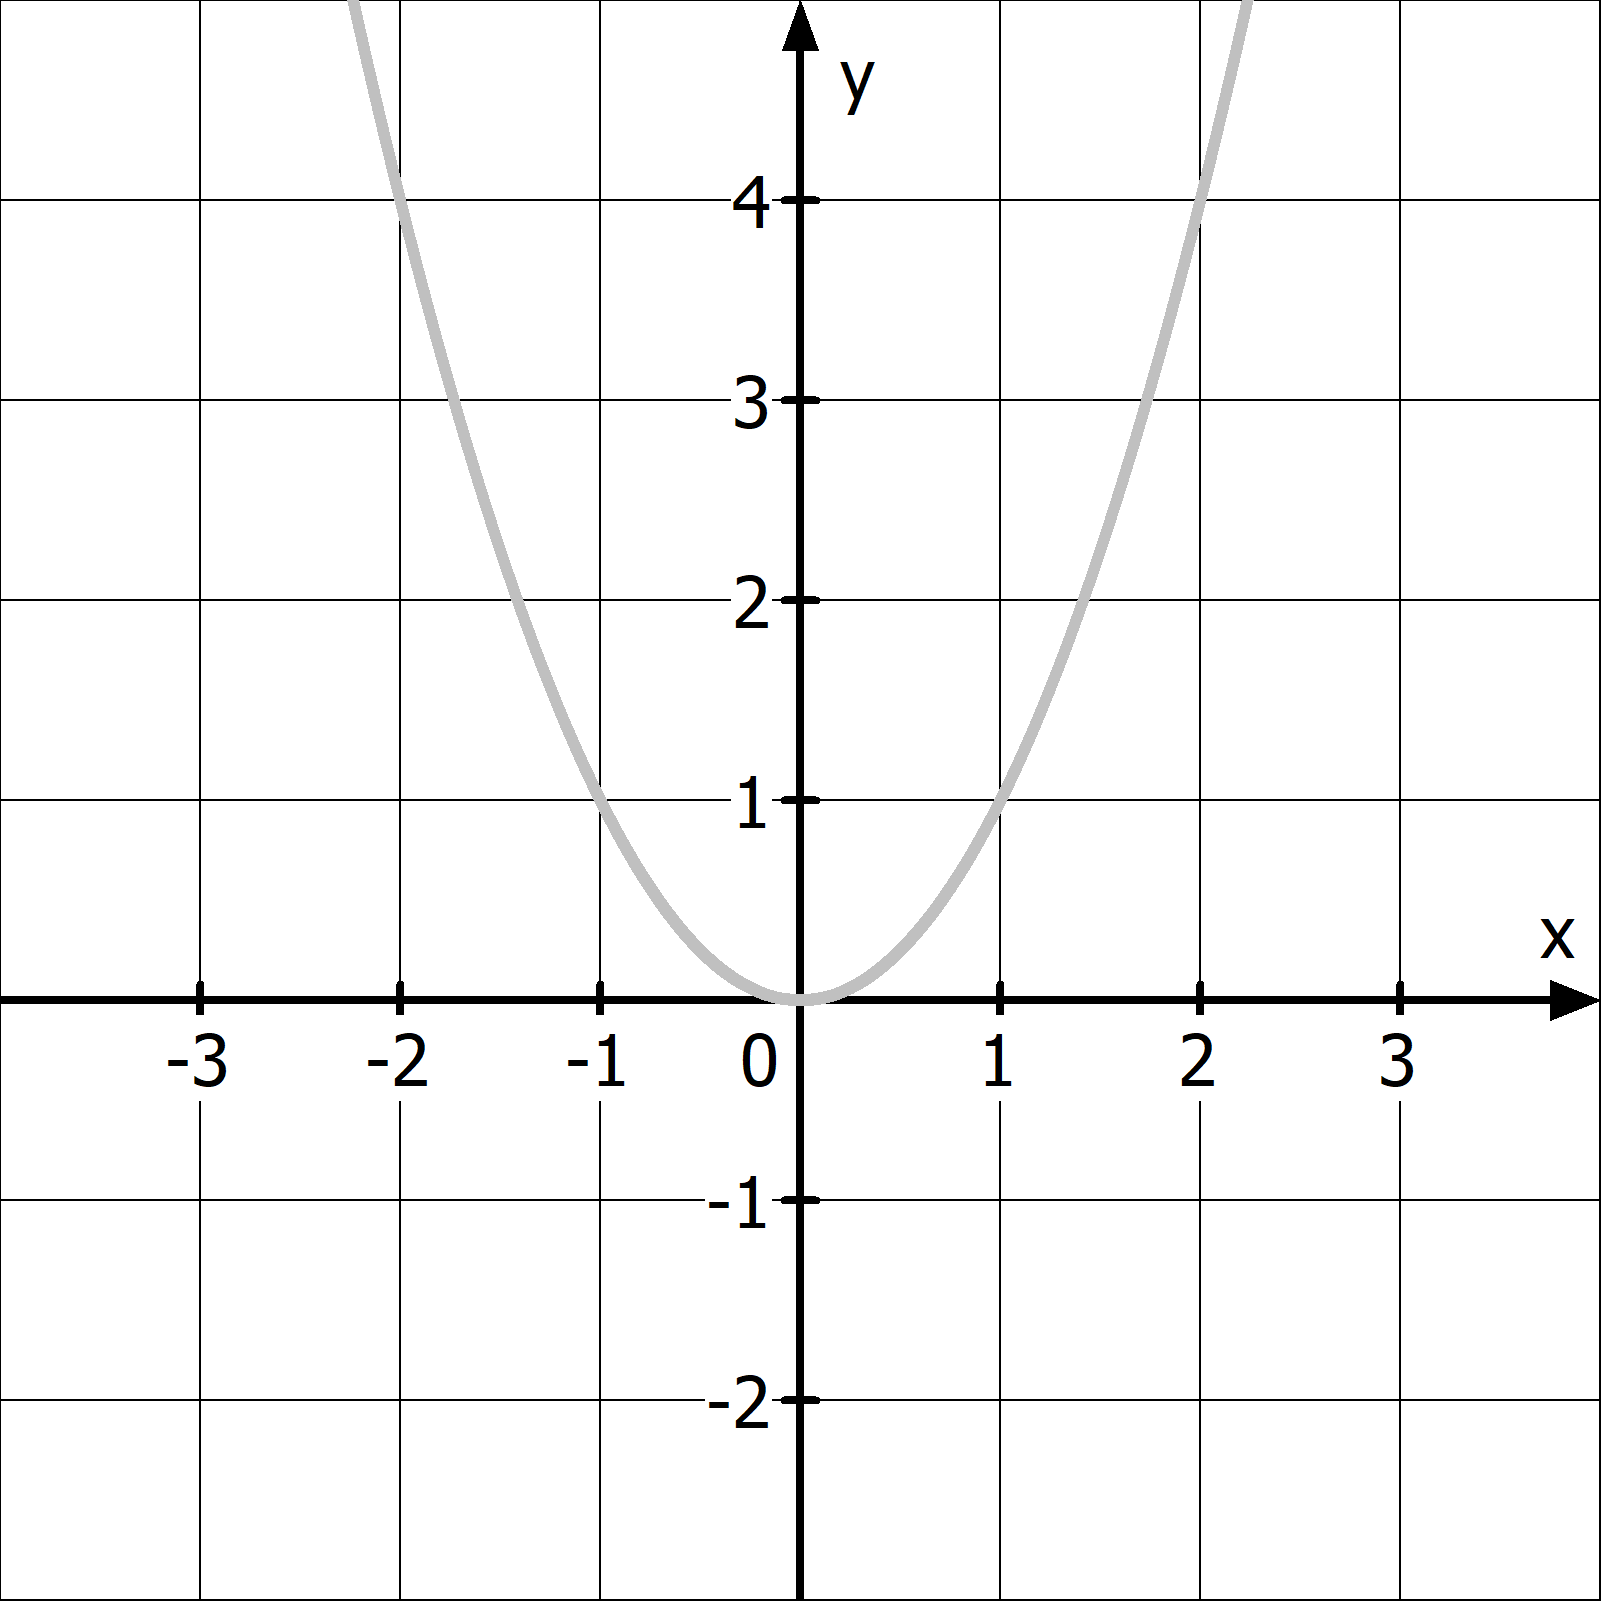
\includegraphics[width=.95\textwidth]{\quadFkt/pics/verschieben_empty.png}
	\end{minipage} \\
\end{tabular}\newpage
\cohead{\Large\textbf{Verschieben in x-Richtung}}
\begin{tabular}{cc}
	\begin{minipage}{0.47\textwidth}
		\centering\Large\textcolor{loes}{Die Normalparabel wird um 2 Einheiten nach rechts verschoben.\newline\newline$f(x)=\left( x-2\right)^2 $\newline\newline Der Scheitel liegt bei $S\left(-2\vert 0\right) $}
	\end{minipage}
	&
	\begin{minipage}{0.47\textwidth}
		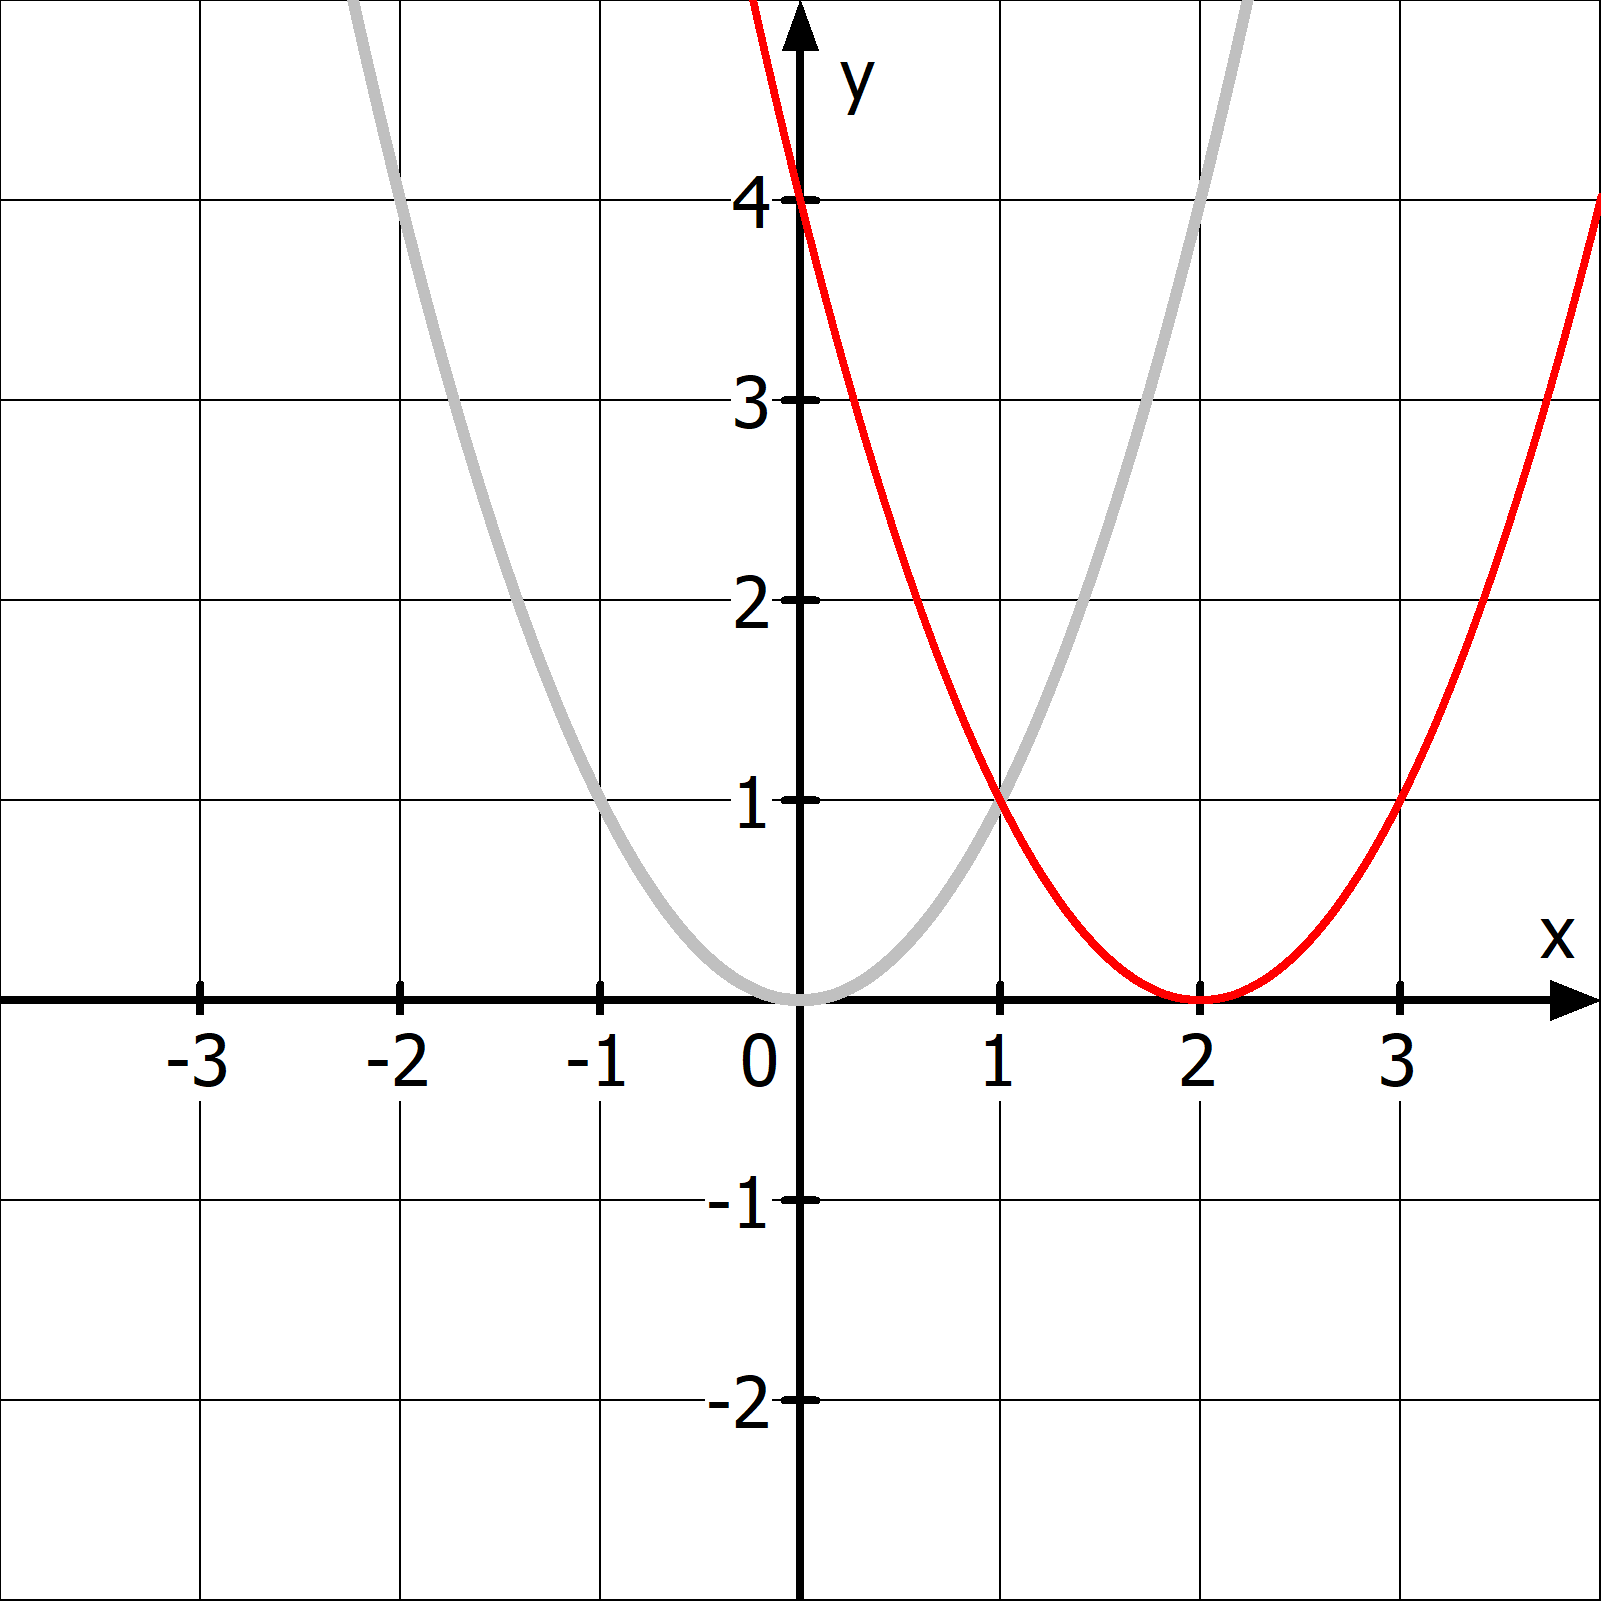
\includegraphics[width=.95\textwidth]{\quadFkt/pics/verschiebenX1.png}
	\end{minipage} \\
	\midrule
	\begin{minipage}{0.47\textwidth}
		\centering\Large Die Normalparabel wird um 1 Einheit nach links verschoben.\newline\newline\textcolor{loes}{$f(x)=\left(x+1 \right)^2 $\newline\newline Der Scheitel liegt bei $S\left(-1\vert 0\right) $}
	\end{minipage}
	&
	\begin{minipage}{0.47\textwidth}
		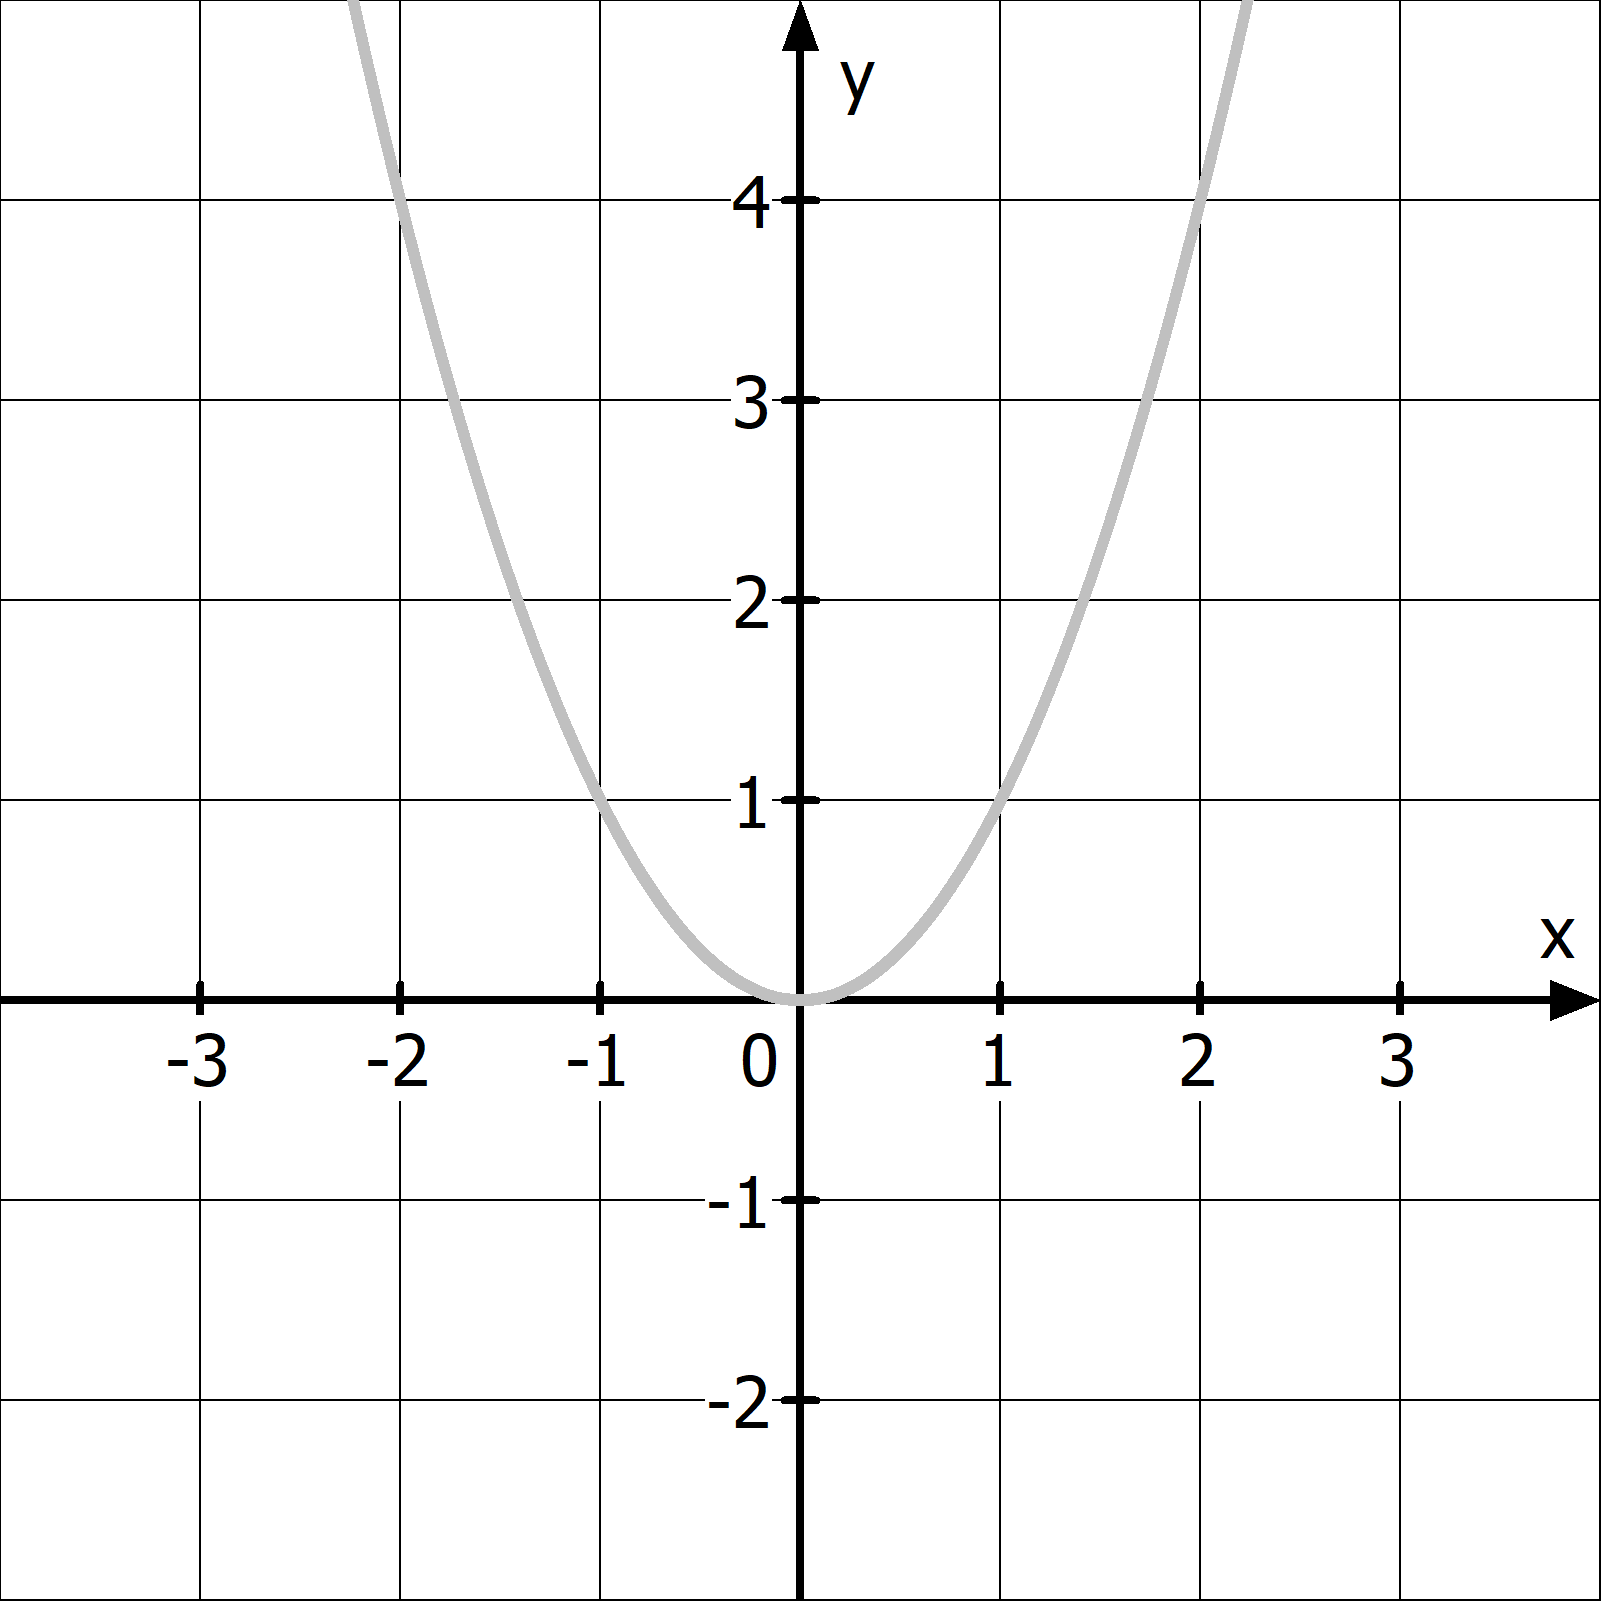
\includegraphics[width=.95\textwidth]{\quadFkt/pics/verschieben_empty.png}
	\end{minipage} \\
	\midrule
	\begin{minipage}{0.47\textwidth}
		\centering\Large\textcolor{loes}{Die Normalparabel wird um 3 Einheiten nach rechts verschoben.}\newline\newline$f(x)=\left( x-3\right)^2$\newline\newline Der Scheitel liegt bei $S\left(3\vert 0\right) $
	\end{minipage}
	&
	\begin{minipage}{0.47\textwidth}
		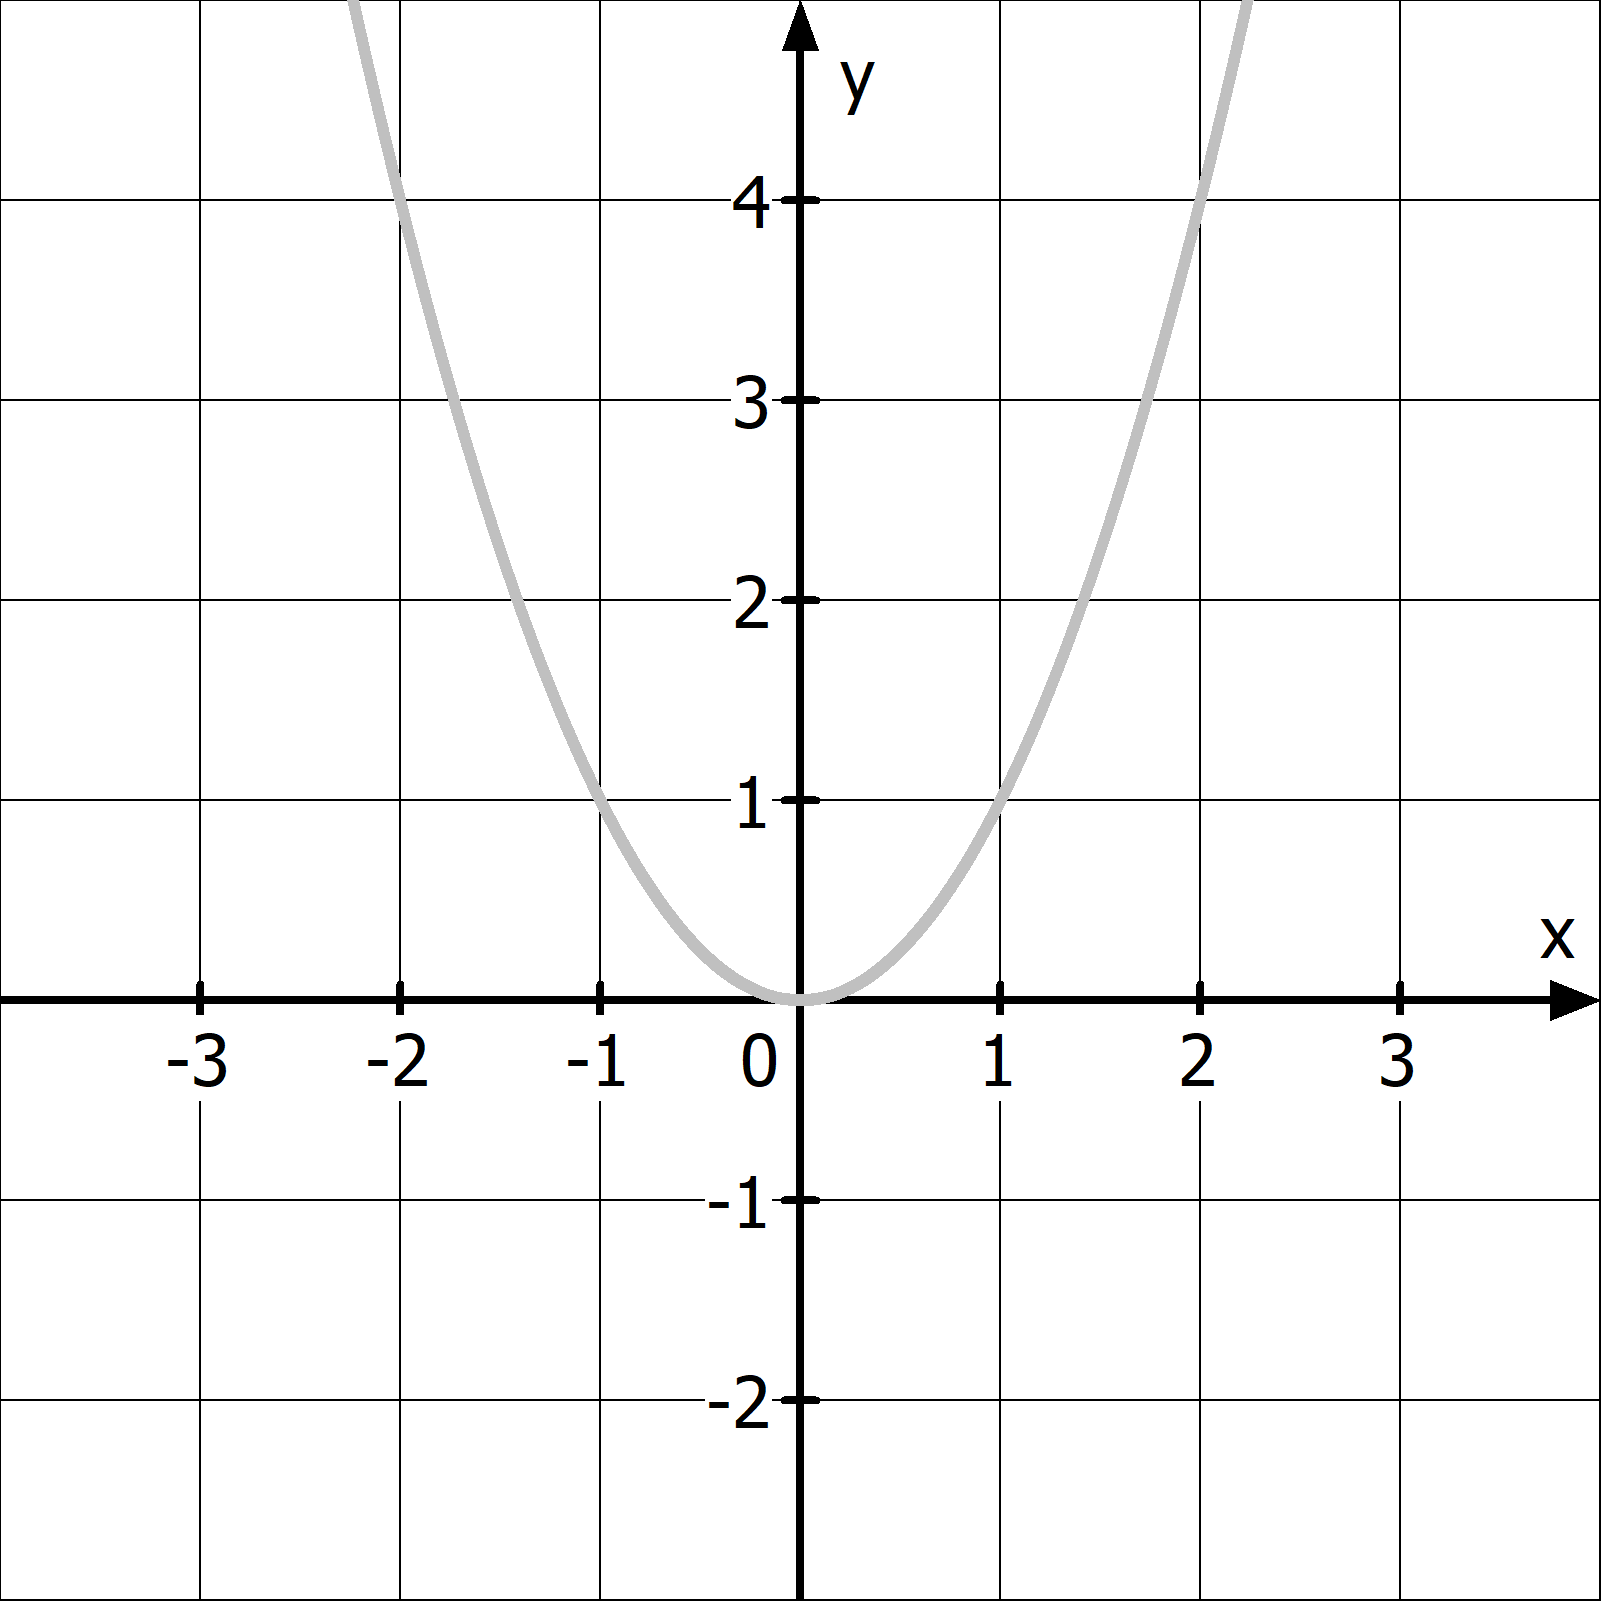
\includegraphics[width=.95\textwidth]{\quadFkt/pics/verschieben_empty.png}
	\end{minipage} \\
\end{tabular}\newpage
%%%%%%%%%%%%%%%%%%%%%%%%%%%%%%%%%%%%%%%%%%%%%%%%%%%%%%%%%%%%%%
\begin{Exercise}[title={Bestimme jeweils an Hand des Schaubilds die Funktionsgleichung}, label=verschiebenA1]
	\begin{minipage}{\linewidth}\centering
		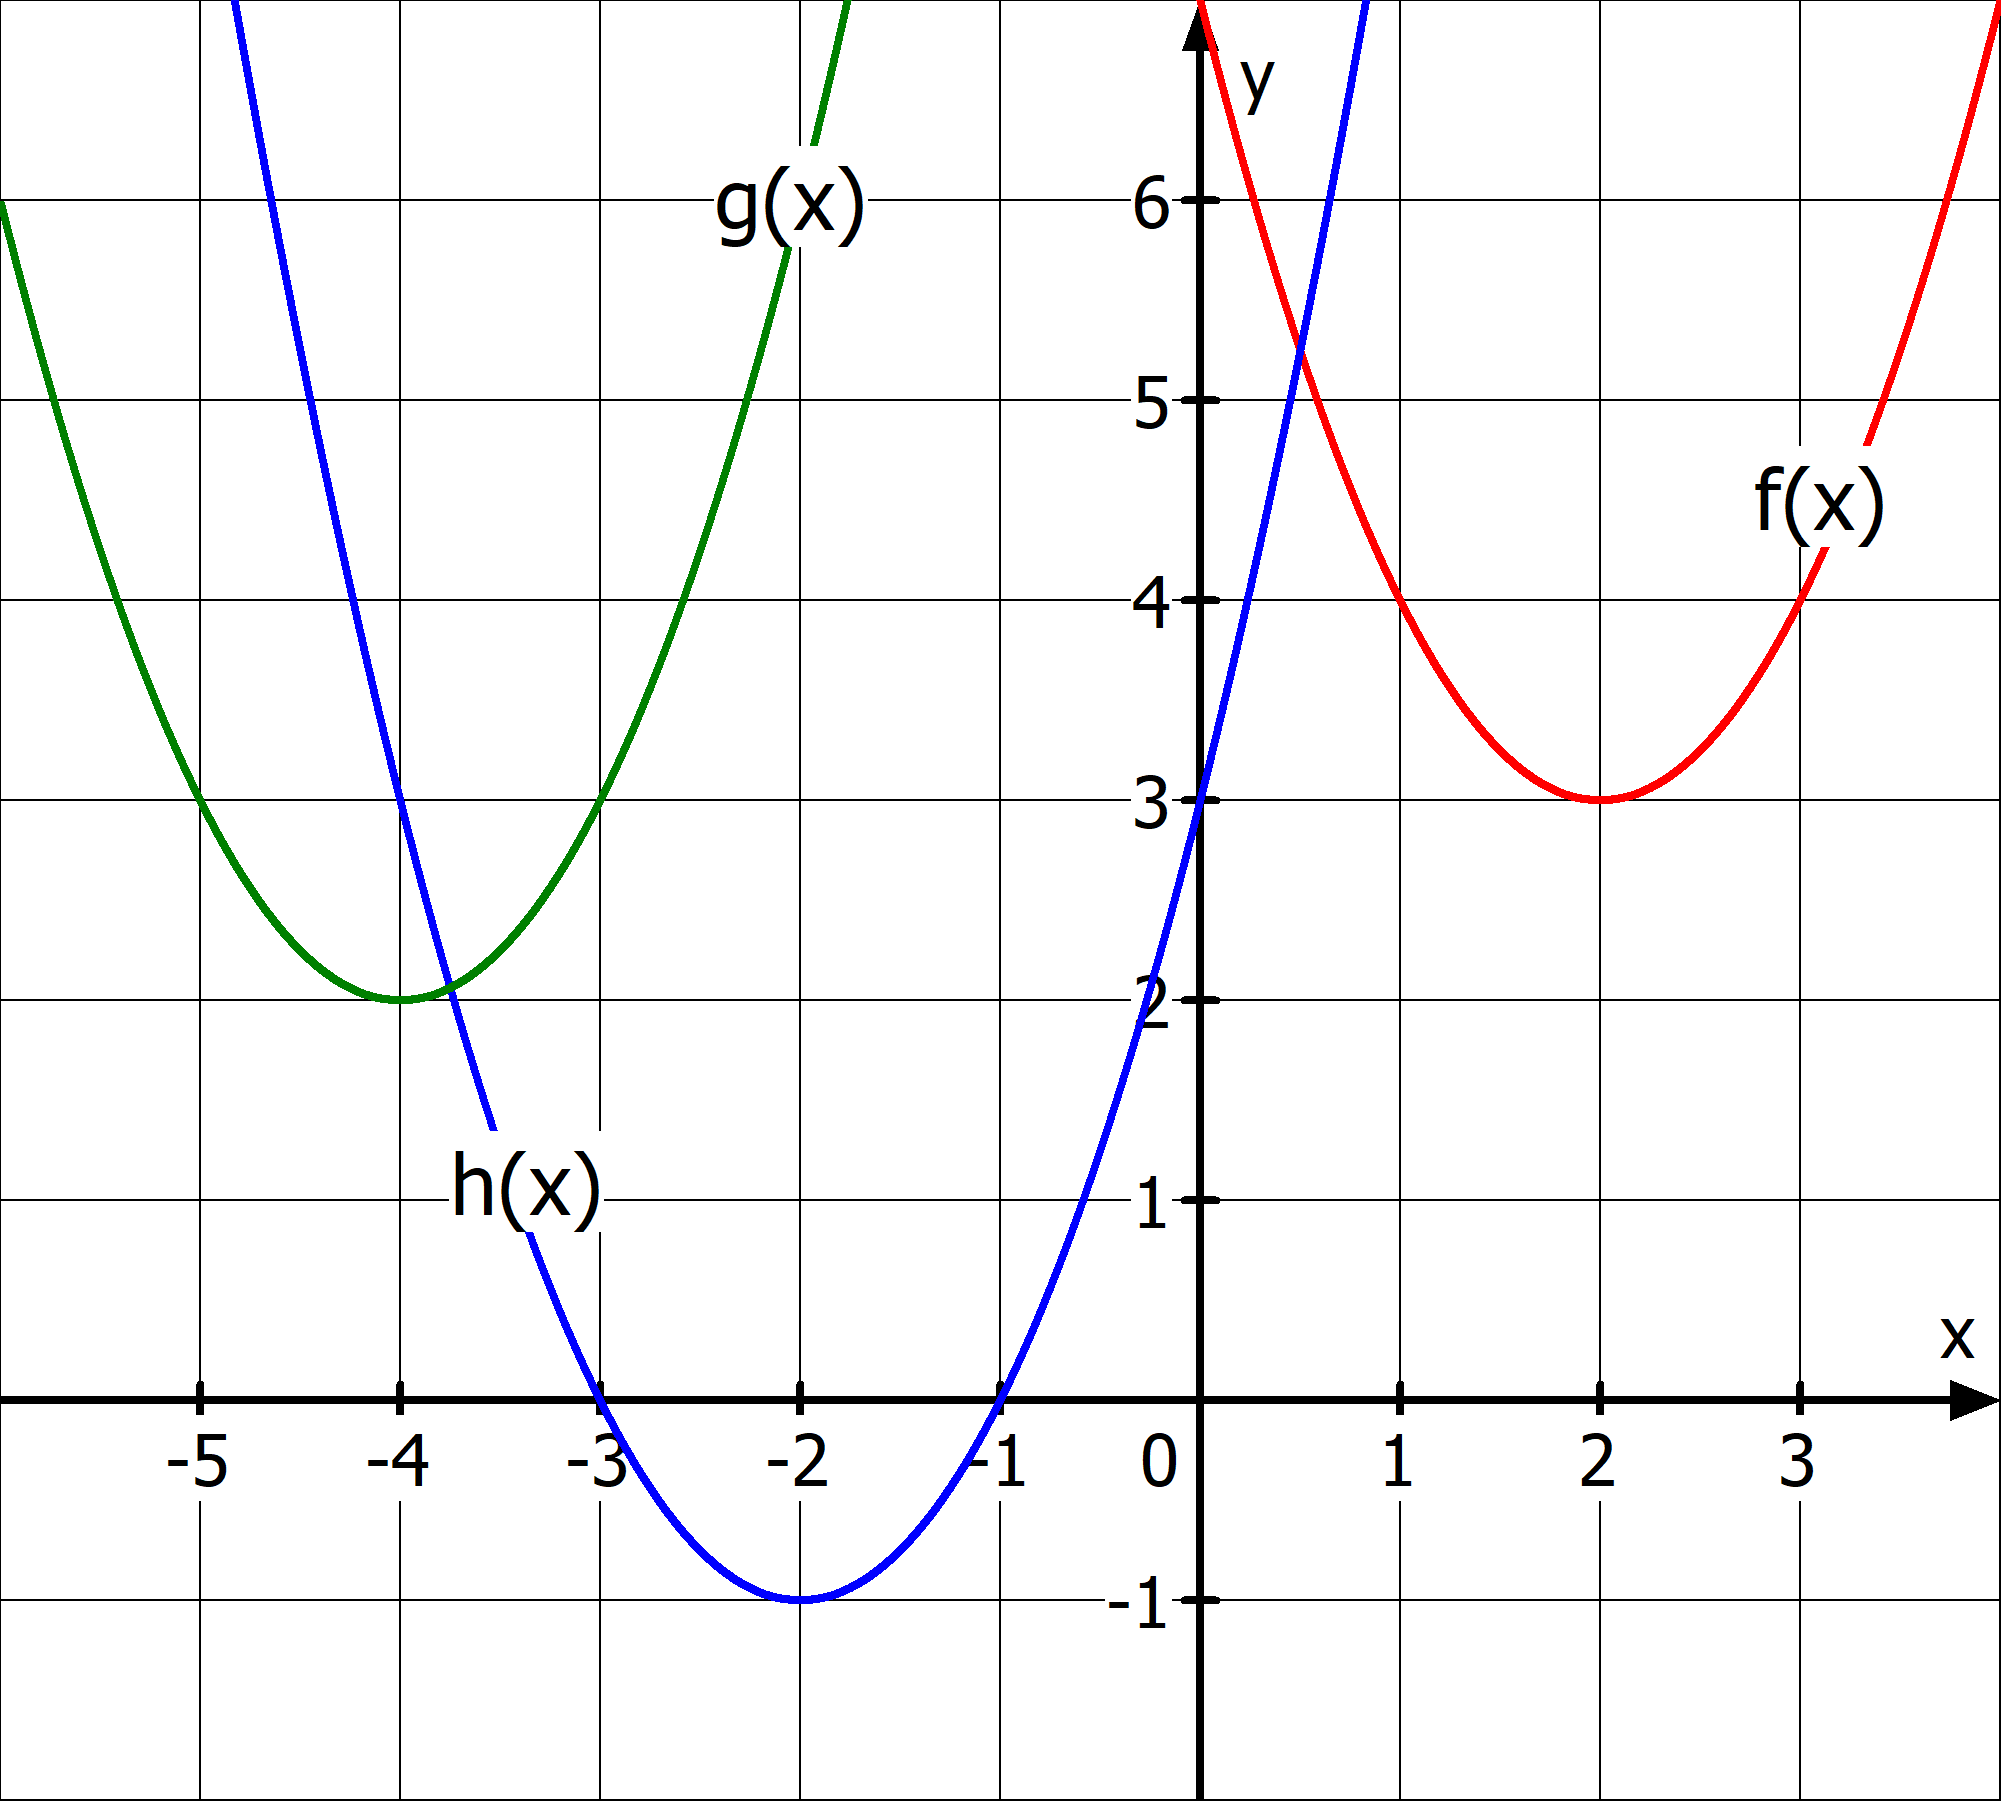
\includegraphics[width=.8\linewidth]{\quadFkt/pics/verschiebenA1.png}
	\end{minipage}
\end{Exercise}

\begin{Exercise}[title={Stelle jeweils die Funktionsgleichung auf und skizziere das Schaubild}, label=verschiebenA2]
	\begin{enumerate}[label=\alph*)]
		\item Die Normalparabel wird um 5 Einheiten nach links und um 3 Einheiten nach unten verschoben.
		\item Die Normalparabel wird um 6 Einheiten nach rechts und um 4 Einheiten nach unten verschoben.
		\item Die Normalparabel wird um 1,5 Einheiten nach links und um 2,5 Einheiten nach oben verschoben.
	\end{enumerate}
\end{Exercise}
\begin{Exercise}[title={Beschreibe wie man die Normalparabel verschieben muss und skizziere das Schaubild}, label=verschiebenA3]
	\begin{enumerate}[label=\alph*)]
		\item $f(x)=(x-3)^2-4$ \quad b) $g(x)=(x+4)^2+3$ \quad c) $h(x)=\left(x-\tfrac{3}{2}\right)^2+\tfrac{5}{2}$
	\end{enumerate}
\end{Exercise}
\begin{Exercise}[title={Stelle die Funktionsgleichung auf}, label=verschiebenA4]
	\begin{enumerate}[label=\alph*)]
		\item Das Schaubild von $f(x)=(x-2)^2+1$ wird um 3 Einheiten nach links und 4 Einheiten nach oben verschoben.
		\item Das Schaubild von $g(x)=(x+3)^2-2$ wird um 4 Einheiten nach rechts und 2 Einheiten nach oben verschoben.
	\end{enumerate}
\end{Exercise}\newpage

\begin{Answer}[ref=verschiebenA1]
	\begin{enumerate}[label=\alph*)]
		\item $f(x)=\left(x+5\right)^2-3$ \quad b) $g(x)=\left(x-6\right)^2-4$ \quad c) $h(x)=\left(x+1,5\right)^2+2,5$
	\end{enumerate}
\end{Answer}

\begin{Answer}[ref=verschiebenA2]\\
	\begin{minipage}{\linewidth}\centering
		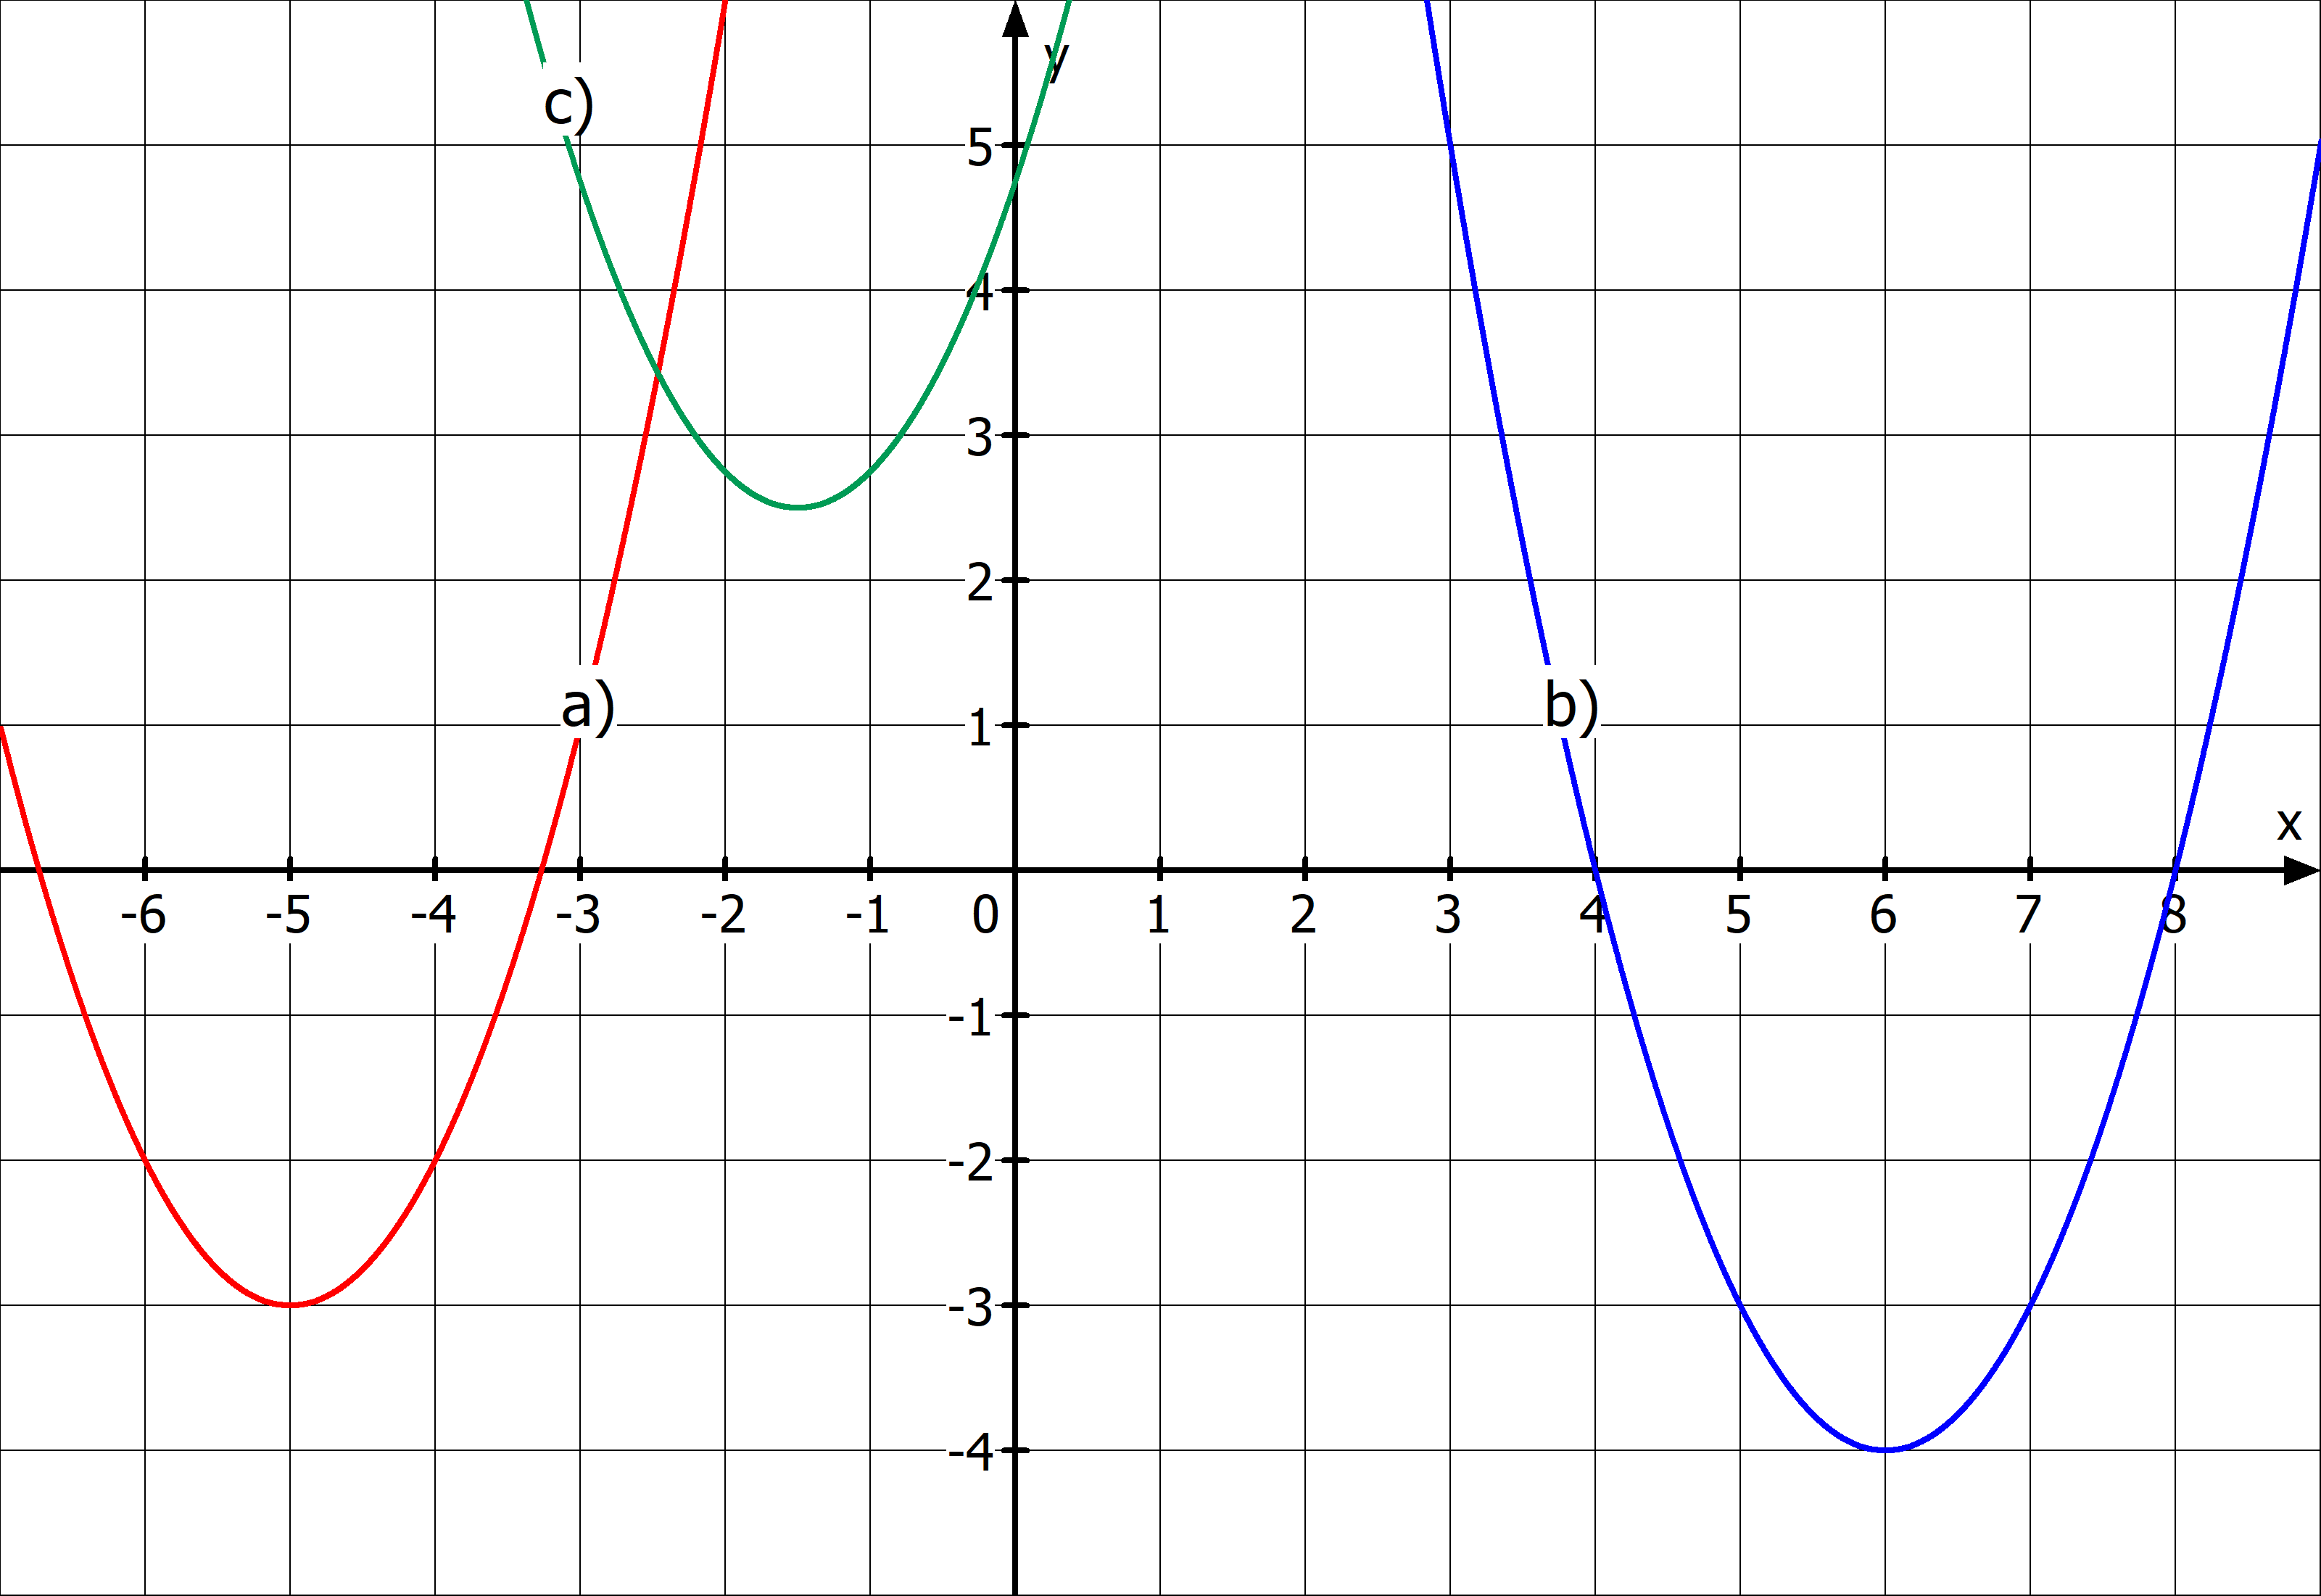
\includegraphics[width=.7\linewidth]{\quadFkt/pics/verschiebenA2.png}
	\end{minipage}\vspace{.1cm}
	\begin{enumerate}[label=\alph*)]
		\item $f(x)=\left(x-2\right)^2+3$ \quad b) $g(x)=\left(x+4\right)^2+2$ \quad c) $h(x)=\left(x+2\right)^2-1$
	\end{enumerate}
\end{Answer}
\begin{Answer}[ref=verschiebenA3]\\
	\begin{minipage}{\linewidth}\centering
		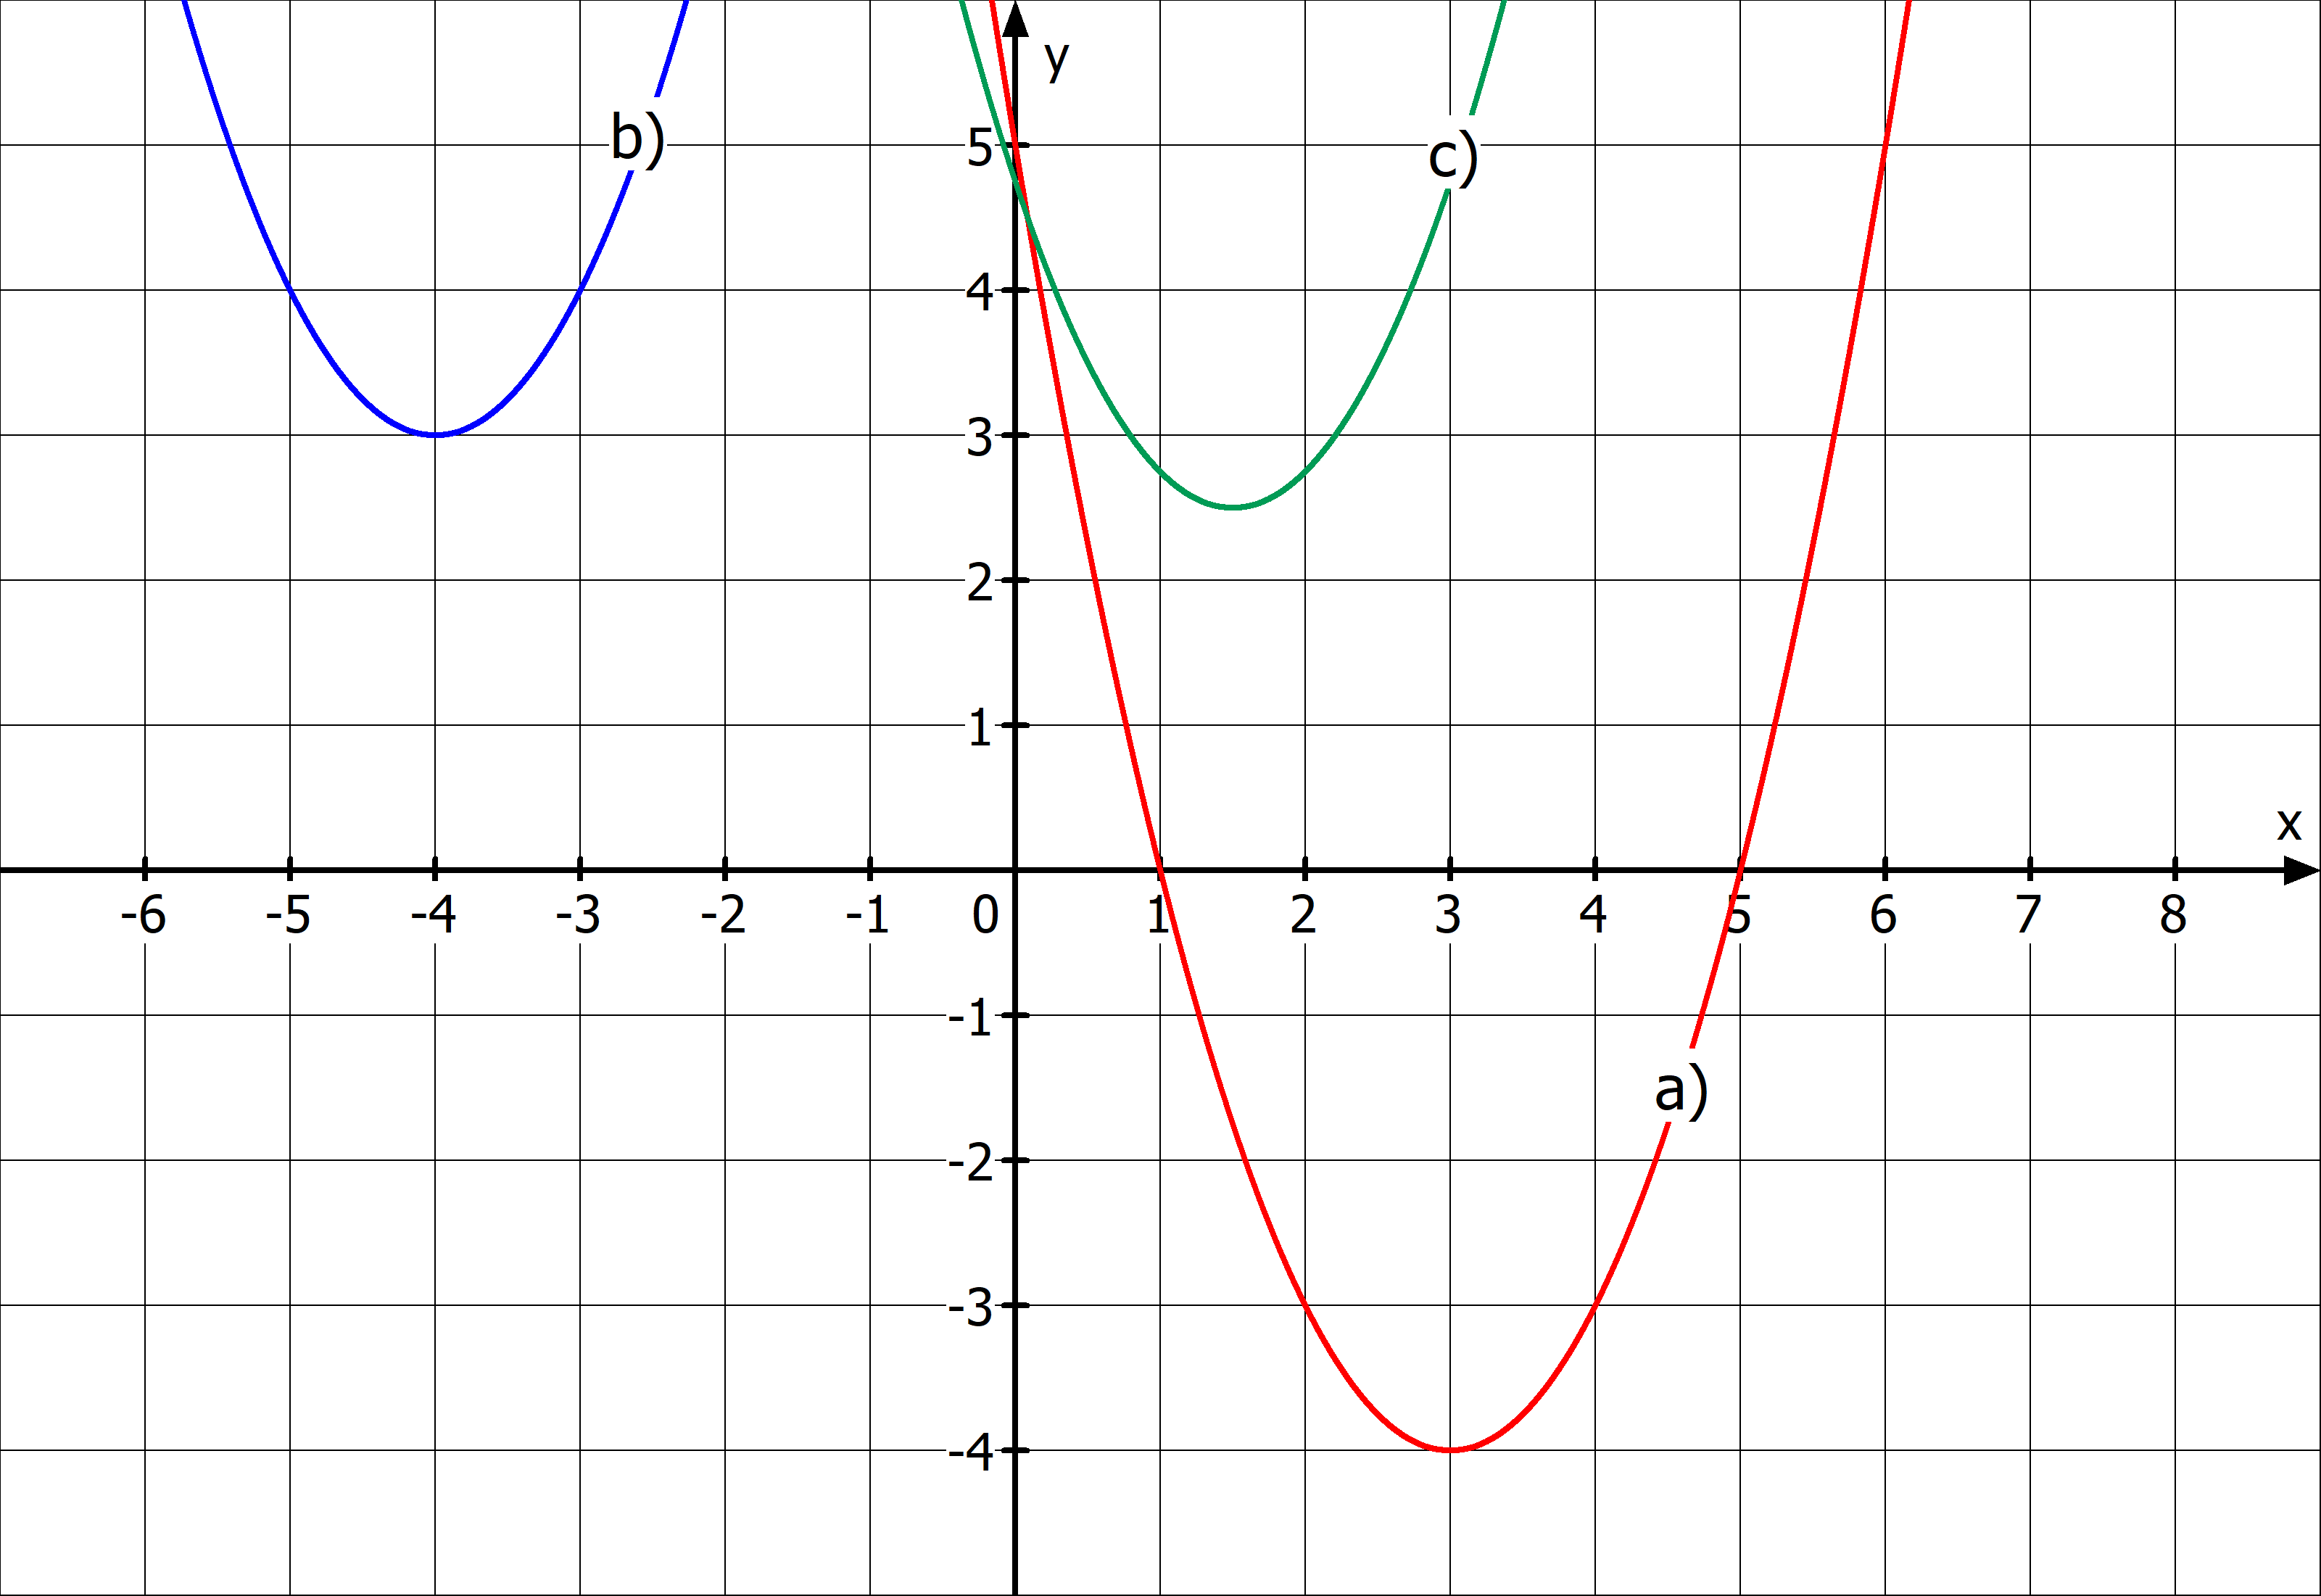
\includegraphics[width=.7\linewidth]{\quadFkt/pics/verschiebenA3.png}
	\end{minipage}\vspace{.1cm}
	\begin{enumerate}[label=\alph*)]
		\item Die Normalparabel wird um 3 Einheiten nach rechts und 4 Einheiten nach unten verschoben.
		\item Die Normalparabel wird um 4 Einheiten nach links und 3 Einheiten nach oben verschoben.
		\item Die Normalparabel wird um 1,5 Einheiten nach rechts und 2,5 Einheiten nach oben verschoben.
	\end{enumerate}
\end{Answer}
\begin{Answer}[ref=verschiebenA4]
	\begin{enumerate}[label=\alph*)]
		\item $f_v(x)=(x+1)^2+5$ \quad b) $g_v(x)=(x-1)^2$
	\end{enumerate}
\end{Answer}\newpage
%%%%%%%%%%%%%%%%%%%%%%%%%%%%%%%%%%%%%%%%
\cohead{\Large\textbf{Strecken und Stauchen}}
\begin{tabular}{cc}
	\begin{minipage}{0.47\textwidth}
		\centering\Large\textcolor{loes}{Die Normalparabel wird mit dem Faktor $2$ gestreckt.\newline\newline$f(x)=2x^2$}
	\end{minipage}
	&
	\begin{minipage}{0.47\textwidth}
		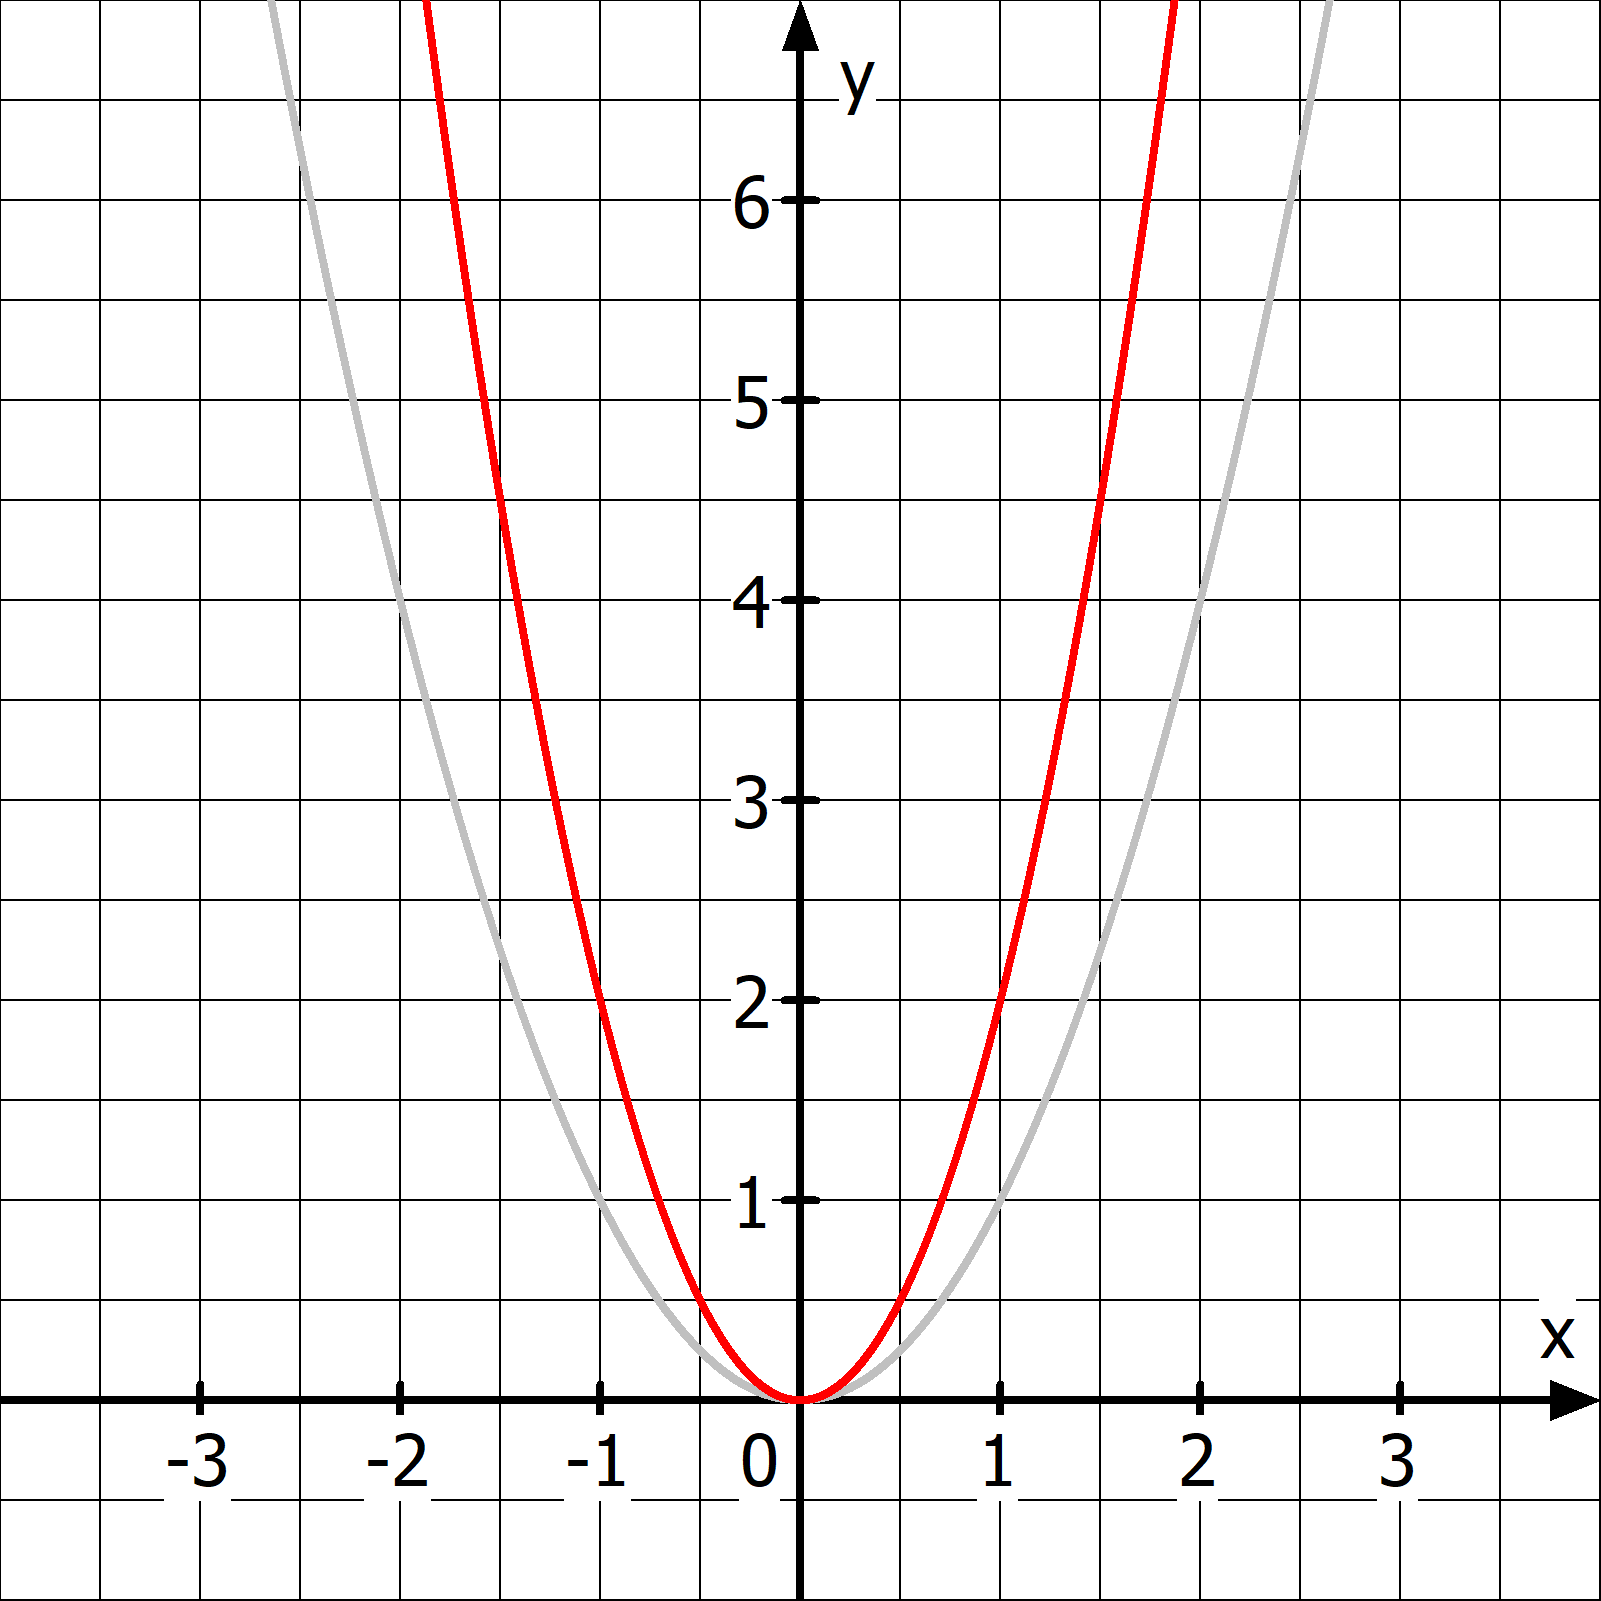
\includegraphics[width=.95\textwidth]{\quadFkt/pics/strecken1.png}
	\end{minipage} \\
	\midrule
	\begin{minipage}{0.47\textwidth}
		\centering\Large Die Normalparabel wird mit dem Faktor $2$ gestaucht oder mit dem Faktor $\tfrac{1}{2}$ gestreckt.\newline\newline\textcolor{loes}{$f(x)=\dfrac{1}{2}x^2$}
	\end{minipage}
	&
	\begin{minipage}{0.47\textwidth}
		\includegraphics[width=.95\textwidth]{\quadFkt/pics/strecken2.png}
	\end{minipage} \\
	\midrule
	\begin{minipage}{0.47\textwidth}
		\centering\Large\textcolor{loes}{Die Normalparabel wird am Scheitel nach unten geklappt und mit dem Faktor $3$ gestaucht oder mit dem Faktor $\tfrac{1}{3}$ gestreckt.}\newline\newline$f(x)=-\tfrac{1}{3}x^2$
	\end{minipage}
	&
	\begin{minipage}{0.47\textwidth}
		\includegraphics[width=.95\textwidth]{\quadFkt/pics/strecken3.png}
	\end{minipage} \\
\end{tabular}\newpage
%%%%%%%%%%%%%%%%%%%%%%%%%%%%%%%%%%%%%%%%%%%%%%%

\begin{Exercise}[title={Bestimme jeweils an Hand des Schaubilds die Funktionsgleichung}, label=scheitelformA1]
	\begin{minipage}{\linewidth}\centering
		\includegraphics[width=\linewidth]{\quadFkt/pics/scheitelA1.png}
	\end{minipage}
\end{Exercise}

\begin{Exercise}[title={Stelle jeweils die Funktionsgleichung auf und skizziere das Schaubild}, label=scheitelformA2]
	\begin{enumerate}[label=\alph*)]
		\item Die Normalparabel wird mit dem Faktor 4 gestreckt um 2 Einheiten nach links und um 4 Einheiten nach unten verschoben.
		\item Die Normalparabel wird mit dem Faktor 0,5 gestreckt, an der x-Achse gespiegelt, um 1 Einheiten nach rechts und um 2 Einheiten nach unten verschoben.
		\item Die Normalparabel wird mit dem Faktor 2 gestreckt, um 2,5 Einheiten nach links, um 3,5 Einheiten nach oben verschoben und zuletzt an der x-Achse gespiegelt.
	\end{enumerate}
\end{Exercise}
\begin{Exercise}[title={Beschreibe wie man die jeweilige Parabel aus der Normalparabel erhält.}, label=scheitelformA3]
	\begin{enumerate}[label=\alph*)]
		\item $f(x)=5(x-1)^2+2$ \quad b) $g(x)=-(x+3)^2-2,5$ \quad c) $h(x)=-\tfrac{2}{3}\left(x-\tfrac{3}{4}\right)^2+\tfrac{5}{7}$
	\end{enumerate}
\end{Exercise}
\begin{Exercise}[title={Stelle die Funktionsgleichung auf}, label=scheitelformA4]
	\begin{enumerate}[label=\alph*)]
		\item Das Schaubild von $f(x)=3(x-4)^2+2$ wird um 5 Einheiten nach links und 2 Einheiten nach oben verschoben und dann an der x-Achse gespiegelt.
		\item Das Schaubild von $g(x)=-(x+2)^2-3$ wird um 5 Einheiten nach rechts und 2 Einheiten nach unten verschoben und dann an der y-Achse gespiegelt.
	\end{enumerate}
\end{Exercise}\newpage

\begin{Answer}[ref=scheitelformA1]
	\begin{enumerate}[label=\alph*)]
		\item \textcolor{red}{$f(x)=\tfrac{1}{4}\left(x-2\right)^2+1$} \quad b) \textcolor{blue}{$g(x)=-2\left(x-3\right)^2-1$} \setcounter{enumi}{2}
		\item \textcolor{ForestGreen}{$h(x)=\tfrac{2}{3}\left(x+3\right)^2-3$} \quad d) \textcolor{YellowOrange}{$i(x)=-\tfrac{3}{4}\left(x+2\right)^2+3$}
	\end{enumerate}
	Hinweis: Bestimme $x_S$ und $y_S$ aus der Position des Scheitels. Den Streckfaktor $a$ kann man dann mittels einer Punktprobe bestimmen (nicht den Scheitel als Punkt verwenden).
\end{Answer}

\begin{Answer}[ref=scheitelformA2]\\
	\begin{minipage}{\linewidth}\centering
		\includegraphics[width=\linewidth]{\quadFkt/pics/scheitelA2.png}
	\end{minipage}\vspace{.1cm}
	\begin{enumerate}[label=\alph*)]
		\item \textcolor{red}{$f(x)=4\left(x+2\right)^2-4$}
		\quad b) \textcolor{blue}{$g(x)=-\tfrac{1}{2}\left(x-1\right)^2-2$} \quad c) \textcolor{ForestGreen}{$h(x)=-2\left(x+2,5\right)^2-3,5$}
	\end{enumerate}
\end{Answer}
\begin{Answer}[ref=scheitelformA3]
	\begin{enumerate}[label=\alph*)]
		\item Die Normalparabel wird mit dem Faktor 5 gestreckt, um 1 Einheit nach rechts und 2 Einheiten nach oben verschoben.
		\item Die Normalparabel wird an der x-Achse gespiegelt, um 3 Einheiten nach links und 2,5 Einheiten nach unten verschoben.
		\item Die Normalparabel wird mit dem Faktor 1,5 gestreckt, an der x-Achse gespiegelt, um 0,75 Einheiten nach rechts und $\tfrac{5}{7}$ Einheiten nach oben verschoben.
	\end{enumerate}
\end{Answer}
\begin{Answer}[ref=scheitelformA4]
	\begin{enumerate}[label=\alph*)]
		\item $f_v(x)=-3\left(x+1\right)^2-4$ \quad b) $g_v(x)=-\left(x+3\right)^2-5$
	\end{enumerate}
\end{Answer}\newpage
	\newpage
	% !TeX root = ../../Skript.tex
\cohead{\Large\textbf{Hauptform ganzrat. Funktionen}}
\fakesubsection{Hauptform ganzrat. Funktionen}
Funktionen, deren Funktionsgleichung man wie folgt darstellen kann, bezeichnet man als ganzrationale Funktionen:

\(f(x)=a_nx^n+a_{n-1}x^{n-1}+a_{n-2}x^{n-2}+\dots +a_2x^2+a_1x+a_0, \quad a_n\neq 0, \quad n\in\N\)

Diese Darstellungsform (komplett ausmultipliziert und zusammengefasst) bezeichnet man als Hauptform oder Normalform.

Folgende Begriffe finden für die ganzrationalen Funktionen Verwendung:
\begin{itemize}\large
	\item[\textcolor{loes}{\textbullet}] \textcolor{loes}{\(n\): Grad der Funktion (größte Hochzahl)}
	\item[\textcolor{loes}{\textbullet}]  \textcolor{loes}{\(a_n,\ a_{n-1},\ a_{n-2}, \dots,\ a_2,\ a_1,\ a_0\): Koeffizienten}
	\item[\textcolor{loes}{\textbullet}]  \textcolor{loes}{\(a_n\): Leitkoeffizient (Koeffizient, der vor dem \(x\) mit der größten Hochzahl steht)}
	\item[\textcolor{loes}{\textbullet}]  \textcolor{loes}{\(a_0\): Absolutglied (immer der Koeffizient, der ohne \(x\) alleine steht)}
\end{itemize}\vspace{2cm}
Beispiele:

\medskip

\begin{minipage}{\textwidth}
	\adjustbox{valign=t}{\begin{minipage}{0.5\textwidth}\raggedright
		\(f(x)=-4x^5+3x^4-\frac{1}{2}x^3+x-3\)

		Grad: \(5\)

		Koeffizienten: \(a_5=-4\), \(a_4=3\), \(a_3=-\frac{1}{2}\),

		\(a_2=0\), \(a_1=1\), \(a_0=-3\)

		Leitkoeffizient \(a_5=-4\)

		Absolutglied \(a_0=-3\)
	\end{minipage}}%
	\adjustbox{valign=t}{\begin{minipage}{0.5\textwidth}\raggedright
		\(g(x)=x^4+2x^3-0,5x\)

		Grad: \textcolor{loes}{\(4\)}

		Koeffizienten: \textcolor{loes}{\(a_4=1\), \(a_3=2\), \(a_2=0\),}

		\textcolor{loes}{\(a_1=-0,5\), \(a_0=0\)}

		Leitkoeffizient \textcolor{loes}{\(a_4=1\)}

		Absolutglied \textcolor{loes}{\(a_0=0\)}
	\end{minipage}}%
\end{minipage}
%%%%%%%%%%%%%%%%%%%%%%%%%%%%%%%%%%%%%%%%%%%%%%%%%%%%%%%%%%%%%%%%%%%%%%%%%%%%%%%%%%%%%%%%%%%%%%%%%%%%%%%%%%%%%%%%%%%%%
\begin{Exercise}[title={Gib den Grad, die Koeffizienten, den Leitkoeffizienten sowie das Absolutglied an.}, label=ganzHauptA1]

	\begin{minipage}{\textwidth}
		\begin{minipage}{0.5\textwidth}
			\begin{enumerate}[label=\alph*)]
				\item \(f(x)=-6x^3+2x-3\)
				\item \(g(x)=0,5x^5-7x^4+2,5x\)
				\item \(h(x)=2x^6\)
				\item \(i(x)=-\frac{3}{2}x^5-8x^4+x^2-1\)
			\end{enumerate}
		\end{minipage}%
		\begin{minipage}{0.5\textwidth}
			\begin{enumerate}[label=\alph*)]
				\setcounter{enumi}{4}
				\item \(j(x)=0,1x^4-12x^3-x^2+8,6x-3,1\)
				\item \(k(x)=-\frac{3}{5}x^7+\frac{2}{7}x^6-\frac{11}{6}x^4-\frac{12}{5}x\)
				\item \(l(x)=2x\left(x^3-2x^2+5\right)\)
				\item \(m(x)=-3x^2\left(x+2\right)^2\)
			\end{enumerate}
		\end{minipage}%
	\end{minipage}%
\end{Exercise}
\newpage
%%%%%%%%%%%%%%%%%%%%%%%%%%%%%%%%%%%%%%%%%
\begin{Answer}[ref=ganzHauptA1]

	\begin{minipage}{\textwidth}
		\begin{minipage}[t]{0.49\textwidth}
			\begin{enumerate}[label=\alph*)]
				\item Grad: \(3\)

				Koeffizienten: \(a_3=-6\), \(a_2=0\), \(a_1=2\), \(a_0=-3\)

				Leitkoeffizient \(a_3=-6\)

				Absolutglied \(a_0=-3\)
				\item Grad: \(5\)

				Koeffizienten: \(a_5=0,5\), \(a_4=-7\), \(a_3=0\), \(a_2=0\), \(a_1=2,5\), \(a_0=0\)

				Leitkoeffizient \(a_5=0,5\)

				Absolutglied \(a_0=0\)
				\item
				Grad: \(6\)

				Koeffizienten: \(a_6=2\), \(a_5=0\), \(a_4=0\), \(a_3=0\), \(a_2=0\), \(a_1=0\), \(a_0=0\)

				Leitkoeffizient \(a_6=2\)

				Absolutglied \(a_0=0\)
				\item Grad: \(5\)

				Koeffizienten: \(a_5=-\frac{3}{2}\), \(a_4=-8\), \(a_3=0\), \(a_2=1\), \(a_1=0\), \(a_0=-1\)

				Leitkoeffizient \(a_5=-\frac{3}{2}\)

				Absolutglied \(a_0=-1\)
			\end{enumerate}
		\end{minipage}%
		\begin{minipage}[t]{0.5\textwidth}
			\begin{enumerate}[label=\alph*)]
				\setcounter{enumi}{4}
				\item Grad: \(4\)

				Koeffizienten: \(a_4=0,1\), \(a_3=-12\),

				\(a_2=-1\), \(a_1=8,6\), \(a_0=-3,1\)

				Leitkoeffizient \(a_4=0,1\)

				Absolutglied \(a_0=-3,1\)
				\item Grad: \(7\)

				Koeffizienten: \(a_7=-\frac{3}{5}\), \(a_6=\frac{2}{7}\), \(a_5=0\), \(a_4=-\frac{11}{6}\), \(a_3=0\), \(a_2=0\), \(a_1=-\frac{12}{5}\), \(a_0=0\)

				Leitkoeffizient \(a_7=-\frac{3}{5}\)

				Absolutglied \(a_0=0\)
				\item \(l(x)=2x\left(x^3-2x^2+5\right)=2x^4-4x^3+10x\)

				Grad: \(4\)

				Koeffizienten: \(a_4=2\), \(a_3=-4\), \(a_2=0\), \(a_1=10\), \(a_0=0\)

				Leitkoeffizient \(a_4=2\)

				Absolutglied \(a_0=0\)
				\item \(m(x)=-3x^2\left(x+2\right)^2\)

				\(\hphantom{m(x)}=-3x^4-12x^3-12x^2\)

				Grad: \(4\)\\
				Koeffizienten: \(a_4=-3\), \(a_3=-12\), \(a_2=-12\),

				\(a_1=0\), \(a_0=0\)

				Leitkoeffizient \(a_4=-3\)

				Absolutglied \(a_0=0\)
			\end{enumerate}
		\end{minipage}%
	\end{minipage}%
\end{Answer}
	\newpage
	\cohead{\Large\textbf{Produktform}}
\fakesubsection{Produktform}
Hat eine ganzrationale Funktion \(f(x)\) vom Grad \(n\) genauso viele Nullstellen wie ihr Grad, so kann man sie in der Produktform darstellen:\\
\(f(x)=a\left(x-x_1 \right)^{n_1} \left(x-x_2 \right)^{n_2}\left(x-x_3 \right)^{n_3} \cdots, \quad a\neq 0, \quad n_1,\ n_2,\ n_3,\ldots\in\N\)\\
Wie auch bei der Produktform der quadratischen Funktionen lassen sich die Nullstellen einfach ablesen. Auch der Leitkoeffizient und der Grad lassen sich leicht bestimmen:
\begin{itemize}\large
	\item[\textcolor{loes}{\textbullet}] \textcolor{loes}{\(x_1,\ x_2,\ x_3,\ldots\): Nullstellen der Funktion}
	\item[\textcolor{loes}{\textbullet}]  \textcolor{loes}{\(n_1,\ n_2,\ n_3,\ldots\): Zu den Nullstellen gehörige Vielfachheiten (VFH) der Nullstellen}
	\item[\textcolor{loes}{\textbullet}]  \textcolor{loes}{\(a\): Leitkoeffizient}
	\item[\textcolor{loes}{\textbullet}]  \textcolor{loes}{\(n_1+n_2+n_3+\cdots\): Die Summe der Vielfachheiten der Nullstellen (oder Anzahl der Nullstellen) entspricht dem Grad der Funktion}
\end{itemize}\vspace{2cm}
Beispiele:\vspace{0.3cm}\\
\begin{minipage}{0.47\textwidth}\raggedright
	\(f(x)=-4\left(x+3\right)^2\left(x+1\right)^3\left(x-2\right)\)\\ \vspace{0.3cm}
	\begin{minipage}{0.8\linewidth}
		\begin{tabular}{rlc}
			\multicolumn{2}{c}{NST}&VFH\\
			\midrule
			\(x_1\hspace{-0.3cm}\)&\(=-3\)&2\\
			\(x_2\hspace{-0.3cm}\)&\(=-1\)&3\\
			\(x_3\hspace{-0.3cm}\)&\(=2\)&1\\
			\phantom{\(x_3\)}&\phantom{\(=2\)}&\phantom{1}
		\end{tabular}
	\end{minipage}\\
	Grad: \(2+3+1=6\)\\
	Leitkoeffizient \(a=-4\)\\
\end{minipage}
\begin{minipage}{0.47\textwidth}\raggedright
	\(g(x)=2\left(x+4\right)\left(x+2\right)^3x^2\left(x-3\right)^2\)\\ \vspace{0.3cm}
	\begin{minipage}{0.8\linewidth}
		\begin{tabular}{rlc}
			\multicolumn{2}{c}{NST}&VFH\\
			\midrule
			\(x_1\hspace{-0.3cm}\)&\(=-4\)&1\\
			\(x_2\hspace{-0.3cm}\)&\(=-2\)&3\\
			\(x_3\hspace{-0.3cm}\)&\(=0\)&2\\
			\(x_4\hspace{-0.3cm}\)&\(=3\)&2
		\end{tabular}
	\end{minipage}\\
	Grad: \(1+3+2+2=8\)\\
	Leitkoeffizient \(a=2\)\\
\end{minipage}\\ \vspace{1cm}

\begin{minipage}{0.47\textwidth}\raggedright
	\(h(x)=\frac{1}{2}\left(x+\frac{3}{2}\right)^4\left(x+\frac{3}{4}\right)\left(x-3\right)^2\)\\ \vspace{0.3cm}
	{\color{loes}\begin{minipage}{0.8\linewidth}
			\begin{tabular}{rlc}
				\multicolumn{2}{c}{NST}&VFH\\
				\midrule
				\(x_1\hspace{-0.3cm}\)&\(=-\frac{3}{2}\)&4\\
				\(x_2\hspace{-0.3cm}\)&\(=-\frac{3}{4}\)&1\\
				\(x_3\hspace{-0.3cm}\)&\(=3\)&2\\
				\phantom{\(x_3\)}&\phantom{\(=2\)}&\phantom{1}
			\end{tabular}
		\end{minipage}\\
		Grad: \(4+1+2=7\)\\
		Leitkoeffizient \(a=\frac{1}{2}\)\\}
\end{minipage}
\begin{minipage}{0.47\textwidth}\raggedright
	\(i(x)=-0,5\left(x+3,5\right)^2\left(x+1,5\right)^2x\left(x-3,8\right)^3\)\\ \vspace{0.3cm}
	{\color{loes}\begin{minipage}{0.8\linewidth}
			\begin{tabular}{rlc}
				\multicolumn{2}{c}{NST}&VFH\\
				\midrule
				\(x_1\hspace{-0.3cm}\)&\(=-3,5\)&2\\
				\(x_2\hspace{-0.3cm}\)&\(=-1,5\)&2\\
				\(x_3\hspace{-0.3cm}\)&\(=0\)&1\\
				\(x_4\hspace{-0.3cm}\)&\(=3,8\)&3
			\end{tabular}
		\end{minipage}\\
		Grad: \(2+2+1+3=8\)\\
		Leitkoeffizient \(a=-0,5\)\\}
\end{minipage}\\
\newpage
%%%%%%%%%%%%%%%%%%%%%%%%%%%%%%%%%%%%%%%%%%%%%%%%%%%%%%%%%%%%%%%%%%%%%%%%%%%%%%%%%%%%%%%%%%%%%%%%%%%%%%%%%%%%%%%%%%%%%
Wir nutzen die Produktform, um Schaubilder zu skizzieren und um ausgehend vom Schaubild die Funktionsgleichung aufzustellen. Die Vielfachheit der Nullstellen gibt an, wie das Schaubild \textbf{in der Nähe} der Nullstelle verläuft.\vspace{0.15cm}\\
\begin{minipage}{\linewidth}
	{\color{loes}\begin{minipage}{0.5\linewidth}
			\textcolor{black}{Beispiel 1: \(f_1(x)=(x+1)x^2(x-2)^3\)}\\
			\begin{tabular}{rlcl}
				\multicolumn{2}{c}{NST}&VFH&Verlauf\\
				\midrule
				\(x_1\hspace{-0.3cm}\)&\(=-1\)&1&wie Gerade\\
				\(x_2\hspace{-0.3cm}\)&\(=0\)&2&Parabelförmig\\
				\(x_3\hspace{-0.3cm}\)&\(=2\)&3&S-förmig
			\end{tabular}\\
			Grad: \(1+2+3=6\)\\
			Leitkoeffizient \(a=1\)\\
	\end{minipage}}
	\begin{minipage}{0.5\linewidth}
		\includegraphics[width=.95\linewidth]{\ganzFkt/pics/produkt1.png}
	\end{minipage}
\end{minipage}\\ \vspace{.15cm}\\
\begin{minipage}{\linewidth}
	\begin{minipage}{0.5\linewidth}
		\includegraphics[width=.95\linewidth]{\ganzFkt/pics/produkt2.png}
	\end{minipage}
	{\color{loes}\begin{minipage}{0.5\linewidth}
			\textcolor{black}{Beispiel 2: \(f_2(x)=-0,5(x+2)^2x(x-1)^2\)}\\
			\begin{tabular}{rlcl}
				\multicolumn{2}{c}{NST}&VFH&Verlauf\\
				\midrule
				\(x_1\hspace{-0.3cm}\)&\(=-2\)&2&Parabelförmig\\
				\(x_2\hspace{-0.3cm}\)&\(=0\)&1&wie Gerade\\
				\(x_3\hspace{-0.3cm}\)&\(=1\)&3&Parabelförmig
			\end{tabular}\\
			Grad: \(2+1+2=2\)\\
			Leitkoeffizient \(a=-0,5\)\\
	\end{minipage}}
\end{minipage}\\ \vspace{.15cm}\\
\begin{minipage}{\linewidth}
	{\color{loes}\begin{minipage}{0.5\linewidth}
			\textcolor{black}{Beispiel 3: \(f_3(x)=-x^3(x-2)\)}\\
			\begin{tabular}{rlcl}
				\multicolumn{2}{c}{NST}&VFH&Verlauf\\
				\midrule
				\(x_1\hspace{-0.3cm}\)&\(=0\)&1&S-förmig\\
				\(x_2\hspace{-0.3cm}\)&\(=2\)&2&wie Gerade
			\end{tabular}\\
			Grad: \(3+1=4\)\\
			Leitkoeffizient \(a=-1\)\\
	\end{minipage}}
	\begin{minipage}{0.5\linewidth}
		\includegraphics[width=.95\linewidth]{\ganzFkt/pics/produkt3.png}
	\end{minipage}
\end{minipage}
\newpage
%%%%%%%%%%%%%%%%%%%%%%%%%%%%%%%%%%%%%%%%%%%%%%%%%%%%%%%%%%%%%%%%%%%%%%%%%%%%%%%%%%%%%%%%%%%%%%%%%%%%%%%%%%%%%%%%%%%%%
Umgekehrt können wir ausgehend vom Schaubild die Funktionsgleichung aufstellen. Sind keine zusätzlichen Angaben zu den Vielfachheiten der Nullstellen gegeben, so probieren wir immer die kleinste mögliche Vielfachheit aus. Damit lässt sich dann die Funktionsgleichung mit Ausnahme des Leitkoeffizienten bestimmen. Dieser lässt sich mit einer Punktprobe berechnen.\vspace{0.15cm}\\
\begin{minipage}{\linewidth}
	{\color{loes}\begin{minipage}{0.5\linewidth}
			\textcolor{black}{Beispiel 1:}\\
			\begin{tabular}{rllc}
				\multicolumn{2}{c}{NST}&Verlauf&VFH\\
				\midrule
				\(x_1\hspace{-0.3cm}\)&\(=-1\)&Parabelförmig&gerade\\
				\(x_2\hspace{-0.3cm}\)&\(=1\)&wie Gerade&1\\
				\(x_3\hspace{-0.3cm}\)&\(=2\)&wie Gerade&1
			\end{tabular}\\
			Nehmen wir für die erste Nullstelle die kleinste mögliche Vielfachheit, also 2, so ergibt sich\\
			\(f_1(x)=a\left(x+1\right)^2 \left(x-1\right) \left(x-2\right) \)\\
			Eine Punktprobe mit \(P(0\vert-1)\), also \(f_1(0)=-1\) ergibt \(a=-0,5\) und damit\\
			\(f_1(x)=-0,5\left(x+1\right)^2 \left(x-1\right) \left(x-2\right) \)
	\end{minipage}}
	\begin{minipage}{0.5\linewidth}
		\includegraphics[width=.95\linewidth]{\ganzFkt/pics/produkt4.png}
	\end{minipage}
\end{minipage}\\ \vspace{.15cm}\\
\begin{minipage}{\linewidth}
	\begin{minipage}{0.5\linewidth}
		\includegraphics[width=.95\linewidth]{\ganzFkt/pics/produkt5.png}
	\end{minipage}
	{\color{loes}\begin{minipage}{0.5\linewidth}
			\textcolor{black}{Beispiel 2:}\\
			\begin{tabular}{rllc}
				\multicolumn{2}{c}{NST}&Verlauf&VFH\\
				\midrule
				\(x_1\hspace{-0.3cm}\)&\(=-2\)&wie Gerade&1\\
				\(x_2\hspace{-0.3cm}\)&\(=0\)&S-förmig&\(3,\ 5,\ \dots\)\\
				\(x_3\hspace{-0.3cm}\)&\(=1\)&wie Gerade&1
			\end{tabular}\\
			Nehmen wir für die zweite Nullstelle die kleinste mögliche Vielfachheit, also 3, so ergibt sich\\
			\(f_2(x)=a\left(x+2\right)x^3 \left(x-1\right) \)\\
			Eine Punktprobe mit \(P(-1\vert 1)\), also \(f_1(-1)=1\) ergibt \(a=0,5\) und damit\\
			\(f_2(x)=0,5\left(x+2\right)x^3 \left(x-1\right) \)
	\end{minipage}}
\end{minipage}\\ \vspace{.15cm}\\
\begin{minipage}{\linewidth}
	{\color{loes}\begin{minipage}{0.5\linewidth}
			\textcolor{black}{Beispiel 3:}\\
			\begin{tabular}{rllc}
				\multicolumn{2}{c}{NST}&Verlauf&VFH\\
				\midrule
				\(x_1\hspace{-0.3cm}\)&\(=0\)&wie Gerade&1\\
				\(x_2\hspace{-0.3cm}\)&\(=2\)&wie Gerade&1\\
				\(x_3\hspace{-0.3cm}\)&\(=3\)&wie Gerade&1
			\end{tabular}\\
			Es ergibt sich aus den Nullstellen:\\
			\(f_3(x)=ax \left(x-2\right) \left(x-3\right) \)\\
			Eine Punktprobe mit \(P(1\vert-2)\), also \(f_1(1)=-2\) ergibt \(a=-1\) und damit\\
			\(f_3(x)=-x \left(x-2\right) \left(x-3\right) \)
	\end{minipage}}
	\begin{minipage}{0.5\linewidth}
		\includegraphics[width=.95\linewidth]{\ganzFkt/pics/produkt6.png}
	\end{minipage}
\end{minipage}
\newpage
%%%%%%%%%%%%%%%%%%%%%%%%%%%%%%%%%%%%%%%%%%%%%%%%%%%%%%%%%%%%%%%%%%%%%%%%%%%%%%%%%%%%%%%%%%%%%%%%%%%%%%%%%%%%%%%%%%%%%
\begin{Exercise}[title={Skizziere das Schaubild}, label=ganzProduktA1]\\
	\begin{minipage}{\textwidth}
		\begin{minipage}{0.49\textwidth}
			\begin{enumerate}[label=\alph*)]
				\item \(f(x)=0,1\left(x+3\right)^2\left(x+1\right)\left(x-1\right)^3\)
				\item \(g(x)=-\frac{1}{5}\left(x+4\right) \left(x+3\right) \left(x+1\right) x^2 \)
				\item \(h(x)=-\left(x+1\right)^3 \left(x-1\right)^2 \left(x-2\right)\)
				\item \(i(x)=\frac{1}{3}x^2\left(x+1\right) \left( x-2\right) \left( x-3\right) ^2\)
			\end{enumerate}
		\end{minipage}
		\begin{minipage}{0.49\textwidth}
			\begin{enumerate}[label=\alph*)]
				\setcounter{enumi}{4}
				\item \(j(x)=\frac{1}{5}\left( x+2\right) x\left( x-2\right) ^2\)
				\item \(k(x)=-x^3\left( x-2\right) ^2\)
				\item \(l(x)=\frac{1}{10}\left( x+4\right) ^2 x^2\)
				\item \(m(x)=-\frac{3}{35}\left( x+5\right) \left( x+4\right) ^2\left( x+2\right) x\)
			\end{enumerate}
		\end{minipage}
	\end{minipage}
\end{Exercise}
\begin{Exercise}[title={Stelle die Funktionsgleichung auf. Verwende jeweils die kleinstmögliche Vielfachheit.}, label=ganzProduktA2]\\
	\begin{minipage}{\textwidth}
		\begin{minipage}{0.49\textwidth}
			\begin{enumerate}[label=\alph*)]
				\item \begin{minipage}[t]{0.95\textwidth}\vspace{-0.5\baselineskip}
					\includegraphics[width=.95\linewidth]{\ganzFkt/pics/produktA2_1.png}
				\end{minipage}\\
				\item \begin{minipage}[t]{0.95\textwidth}\vspace{-0.5\baselineskip}
					\includegraphics[width=.95\linewidth]{\ganzFkt/pics/produktA2_2.png}
				\end{minipage}\\
				\item \begin{minipage}[t]{0.95\textwidth}\vspace{-0.5\baselineskip}
					\includegraphics[width=.95\linewidth]{\ganzFkt/pics/produktA2_3.png}
				\end{minipage}\\
			\end{enumerate}
		\end{minipage}
		\begin{minipage}{0.49\textwidth}
			\begin{enumerate}[label=\alph*)]
				\setcounter{enumi}{3}
				\item \begin{minipage}[t]{0.95\textwidth}\vspace{-0.5\baselineskip}
					\includegraphics[width=.95\linewidth]{\ganzFkt/pics/produktA2_4.png}
				\end{minipage}\\
				\item \begin{minipage}[t]{0.95\textwidth}\vspace{-0.5\baselineskip}
					\includegraphics[width=.95\linewidth]{\ganzFkt/pics/produktA2_5.png}
				\end{minipage}\\
				\item \begin{minipage}[t]{0.95\textwidth}\vspace{-0.5\baselineskip}
					\includegraphics[width=.95\linewidth]{\ganzFkt/pics/produktA2_6.png}
				\end{minipage}\\
			\end{enumerate}
		\end{minipage}
	\end{minipage}
\end{Exercise}\newpage
%%%%%%%%%%%%%%%%%%%%%%%%%%%%%%%%%%%%%%%%%%%%%%%%%%%%%%%%%%%%%%%%%%%%%%%
%%%%%%%%%%%%%%%%%%%%%%%%%%%%%%%%%%%%%%%%%
\begin{Answer}[ref=ganzProduktA1]\\
	\begin{minipage}{\textwidth}
		\begin{minipage}{0.49\textwidth}
			\begin{enumerate}[label=\alph*)]
				\item \(f(x)=0,1\left(x+3\right)^2\left(x+1\right)\left(x-1\right)^3\)\\\begin{minipage}[t]{0.95\textwidth}
					\includegraphics[width=.95\linewidth]{\ganzFkt/pics/produktA1_1.png}
				\end{minipage}
				\item \(g(x)=-\frac{1}{5}\left(x+4\right) \left(x+3\right) \left(x+1\right) x^2 \)\\\begin{minipage}[t]{0.95\textwidth}
					\includegraphics[width=.95\linewidth]{\ganzFkt/pics/produktA1_2.png}
				\end{minipage}
				\item \(h(x)=-\left(x+1\right)^3 \left(x-1\right)^2 \left(x-2\right)\)\\\begin{minipage}[t]{0.95\textwidth}
					\includegraphics[width=.95\linewidth]{\ganzFkt/pics/produktA1_3.png}
				\end{minipage}
				\item \(i(x)=\frac{1}{3}x^2\left(x+1\right) \left( x-2\right) \left( x-3\right) ^2\)\\\begin{minipage}[t]{0.95\textwidth}
					\includegraphics[width=.95\linewidth]{\ganzFkt/pics/produktA1_4.png}
				\end{minipage}
			\end{enumerate}
		\end{minipage}
		\begin{minipage}{0.49\textwidth}
			\begin{enumerate}[label=\alph*)]
				\setcounter{enumi}{4}
				\item \(j(x)=\frac{1}{5}\left( x+2\right) x\left( x-2\right) ^2\)\\\begin{minipage}[t]{0.95\textwidth}
					\includegraphics[width=.95\linewidth]{\ganzFkt/pics/produktA1_5.png}
				\end{minipage}
				\item \(k(x)=-x^3\left( x-2\right) ^2\)\\\begin{minipage}[t]{0.95\textwidth}
					\includegraphics[width=.95\linewidth]{\ganzFkt/pics/produktA1_6.png}
				\end{minipage}
				\item \(l(x)=\frac{1}{10}\left( x+4\right) ^2 x^2\)\\\begin{minipage}[t]{0.95\textwidth}
					\includegraphics[width=.95\linewidth]{\ganzFkt/pics/produktA1_7.png}
				\end{minipage}
				\item \(m(x)=-\frac{3}{35}\left( x+5\right) \left( x+4\right) ^2\left( x+2\right) x\)\\\begin{minipage}[t]{0.95\textwidth}
					\includegraphics[width=.95\linewidth]{\ganzFkt/pics/produktA1_8.png}
				\end{minipage}
			\end{enumerate}
		\end{minipage}
	\end{minipage}
\end{Answer}\newpage
\begin{Answer}[ref=ganzProduktA2]\\
	\begin{minipage}{\textwidth}
		\begin{minipage}[t]{0.49\textwidth}
			\begin{enumerate}[label=\alph*)]
				\item \(f_a(x)=-\frac{1}{6}\left(x+4\right) \left(x+2\right) \left(x-1\right)^2 \)
				\item \(f_b(x)=\left(x+2\right)x^3\left(x-1\right) \)
				\item \(f_c(x)=-\frac{3}{2}x^2\left(x-2\right)^2 \left(x-3\right) \)
			\end{enumerate}
		\end{minipage}
		\begin{minipage}[t]{0.49\textwidth}
			\begin{enumerate}[label=\alph*)]
				\setcounter{enumi}{3}
				\item \(f_d(x)=\frac{1}{2}\left(x+6\right) \left(x+5\right)^2 \left(x+3\right) \)
				\item \(f_e(x)=-\frac{1}{2}x^3\left(x-2\right) \left(x-3\right)^2 \)
				\item \(f_f(x)=\frac{1}{9}\left(x+2\right)^2 x\left(x-2\right)^2 \)
			\end{enumerate}
		\end{minipage}
	\end{minipage}
\end{Answer}
	\newpage
%%	\cohead{\Large\textbf{Lösungen}}
%%	\fakesubsection{Lösungen}
%%	\shipoutAnswer
%%	\newpage
%	%%%%%%%%%%%%%%%%%%%%%%%%%%%%%%%%%%%%%%%%%%%%%%%%%%%%%%%%%%%%%%%%%%%%%%%%%
	\fakesection{Ganzrationale Funktionen}
	\cohead{\Large\textbf{Einführung Exponentialfunktionen}}
\fakesubsection{Einführung Exponentialfunktionen}
Die Anzahl der Bakterien in einer Petrischale verdoppelt sich jede Stunde (bis die komplette Schale mit Bakterien bedeckt ist). Zu Beginn sind 10 Bakterien auf der Schale. Vervollständige die Tabelle:\\
\resizebox{\textwidth}{!}{\begin{tabular}{c||c|c|c|c|c|c|c}
		\(x\)&0&1&2&3&4&5&6\\
		\hline
		\multirow{2}{1cm}{\(f(x)\)}&10&20&\textcolor{loes}{40}&\textcolor{loes}{80}&\textcolor{loes}{160}&\textcolor{loes}{320}&\textcolor{loes}{640}\\
		&\textcolor{loes}{\(10\cdot2^0\)}&\textcolor{loes}{\(10\cdot2^1\)}&\textcolor{loes}{\(10\cdot2^2\)}&\textcolor{loes}{\(10\cdot2^3\)}&\textcolor{loes}{\(10\cdot2^4\)}&\textcolor{loes}{\(10\cdot2^5\)}&\textcolor{loes}{\(10\cdot2^6\)}
\end{tabular}}
\vspace{0.3cm}\\
\begin{minipage}{0.50\textwidth}
	\scalebox{2}{\(f(x)= \textcolor{loes}{10\cdot 2^x}\)}\vspace{0.3cm}\\
	Wie viele Bakterien sind nach 20h und nach 100h vorhanden?\\
	\textcolor{loes}{Da \(x\) die Zeit in Stunden angibt, setzt man einfach die angegebenen Werte ein:}
	\begin{align*}
		\textcolor{loes}{f(20)}&\textcolor{loes}{=10\cdot 2^{20}=10.485.760}\\
		\textcolor{loes}{f(100)}&\textcolor{loes}{=10\cdot 2^{100}\approx 1,27\cdot 10^{31}}
	\end{align*}
	Nach wie vielen Stunden waren 8000 Bakterien vorhanden?\\
	\textcolor{loes}{\(f(x)\) gibt die Anzahl an Bakterien nach \(x\) Stunden an. Wir setzen also gleich:}
	\begin{align*}
		\textcolor{loes}{f(x)}&\textcolor{loes}{=8000}\\
		\textcolor{loes}{10\cdot 2^x}&\textcolor{loes}{=8000\,|\,:10}\\
		\textcolor{loes}{2^x}&\textcolor{loes}{=800\,|\,\log_2}\\
		\textcolor{loes}{\Rightarrow x}&\textcolor{loes}{=\log_2(800)\approx 9,64}
	\end{align*}
	\textcolor{loes}{Der Logarithmus erfüllt für Exponentialfunktionen die gleiche Funktion, die die verschiedenen Wurzeln für \(x^2,\ x^3,\) usw. erfüllen.}\\
\end{minipage}
\begin{minipage}{0.49\textwidth}\centering
	\includegraphics[width=\textwidth]{\eFkt/pics/bakterien_empty.png}
\end{minipage}
Exponentialfunktionen wie \(2^x\) wachsen sehr schnell. Überlegen wir uns zur Illustration wie lange es dauern würde bis die komplette Erde (\(m_{Erde}=6\cdot 10^{24}kg\)) aus Bakterien bestehen würde, falls sie sich unbegrenzt vermehren könnten. 1.000.000.000.000.000 Bakterien wiegen 1g.
\begin{align*}
	\textcolor{loes}{f(x)}&\textcolor{loes}{=6\cdot 10^42}\\
	\textcolor{loes}{10\cdot 2^x}&\textcolor{loes}{=6\cdot 10^42\,|\,:10}\\
	\textcolor{loes}{2^x}&\textcolor{loes}{=6\cdot 10^41\,|\,\log_2}\\
	\textcolor{loes}{\Rightarrow x}&\textcolor{loes}{=\log_2\left( 6\cdot 10^41\right) \approx 138,8}
\end{align*}
\textcolor{loes}{Könnten sich die Bakterien unbegrenzt vermehren, würde es also lediglich \(139h=5,8d\), also nicht ganz 6 Tage, dauern bis die komplette Erde nur aus Bakterien bestehen würde.}
\newpage
%%%%%%%%%%%%%%%%%%%%%%%%%%%%%%%%%%%%%%%%%%%%%%%%%%%%%%%%%%%%%%%%%%%%%%%%%%%%%%%%%%%%%%%%%%%%%%%%%%%%%%
Das Isotop \(^{207}\)Ra hat eine Halbwertszeit von ca. 1s, d.h. dass innerhalb einer Sekunde die Hälfte des radioaktiven Materials in andere Elemente zerfallen ist. Zu Beginn sind 8g Radium vorhanden. Vervollständige die Tabelle:\\
\resizebox{\textwidth}{!}{\begin{tabular}{c||c|c|c|c|c|c|c}
		\(x\)&0&1&2&3&4&5&6\\
		\hline
		\multirow{2}{1cm}{\(f(x)\)}
		&8
		&4
		&\textcolor{loes}{2}
		&\textcolor{loes}{1}
		&\textcolor{loes}{\(\frac{1}{2}\)}
		&\textcolor{loes}{\(\frac{1}{4}\)}
		&\textcolor{loes}{\(\frac{1}{8}\)}\\
		&\textcolor{loes}{\(8\cdot\left(\frac{1}{2}\right)^0\)}
		&\textcolor{loes}{\(8\cdot\left(\frac{1}{2}\right)^1\)}
		&\textcolor{loes}{\(8\cdot\left(\frac{1}{2}\right)^2\)}
		&\textcolor{loes}{\(8\cdot\left(\frac{1}{2}\right)^3\)}
		&\textcolor{loes}{\(8\cdot\left(\frac{1}{2}\right)^4\)}
		&\textcolor{loes}{\(8\cdot\left(\frac{1}{2}\right)^5\)}
		&\textcolor{loes}{\(8\cdot\left(\frac{1}{2}\right)^6\)}
\end{tabular}}
\vspace{0.3cm}\\
\begin{minipage}{0.39\textwidth}
	\scalebox{2}{\(f(x)= \textcolor{loes}{8\cdot \left(\frac{1}{2}\right)^x}\)}\vspace{0.3cm}\\
	Wie viel \(g\) Radium sind nach 10s noch vorhanden, wie viel nach 1min?\\
	\textcolor{loes}{Da \(x\) die Zeit in Sekunden angibt, setzt man einfach die angegebenen Werte ein:}
	\begin{align*}
		\textcolor{loes}{f(10)}&\textcolor{loes}{=8\cdot \left(\frac{1}{2}\right)^{10}=\frac{1}{128}\approx 0,00781}\\
		\textcolor{loes}{f(60)}&\textcolor{loes}{=8\cdot \left(\frac{1}{2}\right)^{60}=\frac{1}{128}\approx 6,94\cdot10^{-18}}
	\end{align*}
	\vfill
\end{minipage}
\begin{minipage}{0.6\textwidth}\centering
	\includegraphics[width=\textwidth]{\eFkt/pics/radium_empty.png}
\end{minipage}\vspace{0.3cm}\\
Nach wie vielen Sekunden waren noch 0,3g Radium vorhanden?\\
\textcolor{loes}{\(f(x)\) gibt die Masse des Radiums in \(g\) nach \(x\) Sekunden an. Wir setzen also gleich:}
\begin{align*}
	\textcolor{loes}{f(x)}&\textcolor{loes}{=0,3}\\
	\textcolor{loes}{8\cdot \left(\frac{1}{2}\right)^x}&\textcolor{loes}{=0,3\,|\,:8}\\
	\textcolor{loes}{\left(\frac{1}{2}\right)^x}&\textcolor{loes}{=\frac{3}{80}\,|\,\log_{\frac{1}{2}}}\\
	\textcolor{loes}{\Rightarrow x}&\textcolor{loes}{=\log_{\frac{1}{2}}\left(\frac{3}{80}\right) \approx 4,74}
\end{align*}
Wie lange würde es dauern bis die Masse des Radiums die eines Bakteriums entspricht?
\begin{align*}
	\textcolor{loes}{f(x)}&\textcolor{loes}{=10^{-15}}\\
	\textcolor{loes}{8\cdot \left(\frac{1}{2}\right)^x}&\textcolor{loes}{=10^{-15}\,|\,:8}\\
	\textcolor{loes}{\left(\frac{1}{2}\right)^x}&\textcolor{loes}{=1,25\cdot 10^{-16}\,|\,\log_{\frac{1}{2}}}\\
	\textcolor{loes}{\Rightarrow x}&\textcolor{loes}{=\log_{\frac{1}{2}}\left(1,25\cdot 10^{-16}\right) \approx 52,8}
\end{align*}
\textcolor{loes}{Es dauert also nicht mal ganz eine Minute bis das Radium fast verschwunden ist.}
	\newpage
	\cohead{\Large\textbf{Potenzfunktionen}}
\fakesubsection{Potenzfunktionen}
\setlength{\qrheight}{2.5cm}%
\newlength{\potenzfunktionenLength}%
\iftoggle{qrcode}{\setlength{\potenzfunktionenLength}{\textwidth-\qrheight}}{\setlength{\potenzfunktionenLength}{\textwidth}}%
\begin{minipage}{\textwidth}
\adjustbox{valign=t}{\begin{minipage}{\potenzfunktionenLength}
    Funktionen vom Typ
    \[f(x)=a\cdot x^n, \quad a\neq 0, \quad n\in\N\]
    bezeichnen wir als Potenzfunktionen.

    Der Koeffizient \(a\) ist der Streckfaktor, wie wir ihn bereits von quadratischen Funktionen kennen.

    Die Hochzahl bzw. der Exponent \(n\) ist eine natürliche Zahl: \(\N=\{1,\,2,\,3,\,4,\,\dots\}\)

    Die Schaubilder der Potenzfunktionen teilen sich in drei verschiedene Formen auf:
\end{minipage}}%
\iftoggle{qrcode}{%
    \adjustbox{valign=t}{\begin{minipage}{\qrheight}
            \href{https://www.geogebra.org/m/rp8rtgpv}{\includegraphics[height=\qrheight]{\ganzFkt/pics/PotenzfunktionenQR.png}}%
    \end{minipage}}%
}{}%
\end{minipage}

\bigskip

\begin{minipage}{\textwidth}

	\begin{minipage}{0.65\textwidth}
		\centering\Large\textcolor{loes}{Für \(n=1\) ergibt sich eine Gerade.}
	\end{minipage}%
	\begin{minipage}{0.35\textwidth}
		\includegraphics[width=\linewidth]{\ganzFkt/pics/potenzGerade.png}
	\end{minipage}%

	\bigskip

	\begin{minipage}{0.65\textwidth}
		\centering\Large\textcolor{loes}{Gerade Hochzahlen: \(x^2,\ x^4,\ x^6,\ \dots\)}

			\textcolor{loes}{Parabelförmig}

			\textcolor{loes}{Achsensymmetrie zur y-Achse}

			\textcolor{loes}{\(f(x)\xrightarrow{\hphantom{\ }x\to-\infty\hphantom{\ }}\infty\)}

			\textcolor{loes}{\(f(x)\xrightarrow{\hphantom{\ }x\to\infty\hphantom{\ }}\infty\)}
	\end{minipage}%
	\begin{minipage}{0.35\textwidth}
		\includegraphics[width=\linewidth]{\ganzFkt/pics/potenzGeradeHZ.png}
	\end{minipage}%

	\bigskip

	\begin{minipage}{0.65\textwidth}
		\centering\Large\textcolor{loes}{Ungerade Hochzahlen (größer 1): \(x^3,\ x^5,\ x^7,\ \dots\)}

			\textcolor{loes}{S-förmig}

			\textcolor{loes}{Punktsymmetrie zum Ursprung}

			\textcolor{loes}{\(f(x)\xrightarrow{\hphantom{\ }x\to-\infty\hphantom{\ }}-\infty\)}

			\textcolor{loes}{\(f(x)\xrightarrow{\hphantom{\ }x\to\infty\hphantom{\ }}\infty\)}
	\end{minipage}%
	\begin{minipage}{0.35\textwidth}
		\includegraphics[width=\linewidth]{\ganzFkt/pics/potenzUngeradeHZ.png}
	\end{minipage}%
\end{minipage}
\newpage
%%%%%%%%%%%%%%%%%%%%%%%%%%%%%%%%%%%%%%%%%%%%%%%%%%%%%%%%%%%%%%%%%%%%%%%%%%%%%%%%%%%%%%%%%%%%%%%%%%%%%%%%%%%%%%%%%%%%%
\begin{Exercise}[title={Skizziere das Schaubild, gib die Symmetrie sowie das Verhalten für sehr große/kleine \(x\) an.}, label=potenzA1]

	\begin{minipage}{\textwidth}
		\begin{minipage}{0.5\textwidth}
			\begin{enumerate}[label=\alph*)]
				\item \(f(x)=-x^2\)
				\item \(g(x)=0,5x^3\)
				\item \(h(x)=2x^6\)
				\item \(i(x)=-\frac{3}{2}x^5\)
			\end{enumerate}
		\end{minipage}%
		\begin{minipage}{0.5\textwidth}
			\begin{enumerate}[label=\alph*)]
				\setcounter{enumi}{4}
				\item \(j(x)=0,1x^4\)
				\item \(k(x)=-\frac{3}{5}x^7\)
				\item \(l(x)=-\sqrt{2}x^4\)
				\item \(m(x)=3x^5\)
			\end{enumerate}
		\end{minipage}%
	\end{minipage}%
\end{Exercise}
\newpage
%%%%%%%%%%%%%%%%%%%%%%%%%%%%%%%%%%%%%%%%%
\begin{Answer}[ref=potenzA1]

	Relevant ist nur, ob die Hochzahl gerade/ungerade ist sowie das Vorzeichen des Streckfaktors:

	\bigskip

	\begin{minipage}{\textwidth}
		\begin{minipage}{0.5\textwidth}\centering
			\(a\) positiv und \(n\) gerade wie \(h(x)\) und \(j(x)\)

			Parabelförmig

			Achsensymmetrie zur y-Achse

			\(f(x)\xrightarrow{\hphantom{\ }x\to-\infty\hphantom{\ }}\infty\)

			\(f(x)\xrightarrow{\hphantom{\ }x\to\infty\hphantom{\ }}\infty\)

			\includegraphics[width=.95\linewidth]{\ganzFkt/pics/potenzPosGerA1.png}
		\end{minipage}%
		\begin{minipage}{0.5\textwidth}\centering
			\(a\) negativ und \(n\) gerade wie \(f(x)\) und \(l(x)\)\\
			Parabelförmig

			Achsensymmetrie zur y-Achse

			\(f(x)\xrightarrow{\hphantom{\ }x\to-\infty\hphantom{\ }}-\infty\)

			\(f(x)\xrightarrow{\hphantom{\ }x\to\infty\hphantom{\ }}-\infty\)

			\includegraphics[width=.95\linewidth]{\ganzFkt/pics/potenzNegGerA1.png}
		\end{minipage}%

		\bigskip

		\begin{minipage}{0.5\textwidth}\centering
			\(a\) positiv und \(n\) ungerade wie \(g(x)\) und \(m(x)\)

			S-förmig

			Punktsymmetrie zum Ursprung\\
			\(f(x)\xrightarrow{\hphantom{\ }x\to-\infty\hphantom{\ }}-\infty\)

			\(f(x)\xrightarrow{\hphantom{\ }x\to\infty\hphantom{\ }}\infty\)

			\includegraphics[width=.95\linewidth]{\ganzFkt/pics/potenzPosUngerA1.png}
		\end{minipage}%
		\begin{minipage}{0.5\textwidth}\centering
			\(a\) negativ und \(n\) ungerade wie \(i(x)\) und \(k(x)\)

			S-förmig

			Punktsymmetrie zum Ursprung

			\(f(x)\xrightarrow{\hphantom{\ }x\to-\infty\hphantom{\ }}\infty\)

			\(f(x)\xrightarrow{\hphantom{\ }x\to\infty\hphantom{\ }}-\infty\)

			\includegraphics[width=.95\linewidth]{\ganzFkt/pics/potenzNegUngerA1.png}
		\end{minipage}%
	\end{minipage}
\end{Answer}
	\newpage
	% !TeX root = ../../Skript.tex
\cohead{\Large\textbf{Hauptform ganzrat. Funktionen}}
\fakesubsection{Hauptform ganzrat. Funktionen}
Funktionen, deren Funktionsgleichung man wie folgt darstellen kann, bezeichnet man als ganzrationale Funktionen:

\(f(x)=a_nx^n+a_{n-1}x^{n-1}+a_{n-2}x^{n-2}+\dots +a_2x^2+a_1x+a_0, \quad a_n\neq 0, \quad n\in\N\)

Diese Darstellungsform (komplett ausmultipliziert und zusammengefasst) bezeichnet man als Hauptform oder Normalform.

Folgende Begriffe finden für die ganzrationalen Funktionen Verwendung:
\begin{itemize}\large
	\item[\textcolor{loes}{\textbullet}] \textcolor{loes}{\(n\): Grad der Funktion (größte Hochzahl)}
	\item[\textcolor{loes}{\textbullet}]  \textcolor{loes}{\(a_n,\ a_{n-1},\ a_{n-2}, \dots,\ a_2,\ a_1,\ a_0\): Koeffizienten}
	\item[\textcolor{loes}{\textbullet}]  \textcolor{loes}{\(a_n\): Leitkoeffizient (Koeffizient, der vor dem \(x\) mit der größten Hochzahl steht)}
	\item[\textcolor{loes}{\textbullet}]  \textcolor{loes}{\(a_0\): Absolutglied (immer der Koeffizient, der ohne \(x\) alleine steht)}
\end{itemize}\vspace{2cm}
Beispiele:

\medskip

\begin{minipage}{\textwidth}
	\adjustbox{valign=t}{\begin{minipage}{0.5\textwidth}\raggedright
		\(f(x)=-4x^5+3x^4-\frac{1}{2}x^3+x-3\)

		Grad: \(5\)

		Koeffizienten: \(a_5=-4\), \(a_4=3\), \(a_3=-\frac{1}{2}\),

		\(a_2=0\), \(a_1=1\), \(a_0=-3\)

		Leitkoeffizient \(a_5=-4\)

		Absolutglied \(a_0=-3\)
	\end{minipage}}%
	\adjustbox{valign=t}{\begin{minipage}{0.5\textwidth}\raggedright
		\(g(x)=x^4+2x^3-0,5x\)

		Grad: \textcolor{loes}{\(4\)}

		Koeffizienten: \textcolor{loes}{\(a_4=1\), \(a_3=2\), \(a_2=0\),}

		\textcolor{loes}{\(a_1=-0,5\), \(a_0=0\)}

		Leitkoeffizient \textcolor{loes}{\(a_4=1\)}

		Absolutglied \textcolor{loes}{\(a_0=0\)}
	\end{minipage}}%
\end{minipage}
%%%%%%%%%%%%%%%%%%%%%%%%%%%%%%%%%%%%%%%%%%%%%%%%%%%%%%%%%%%%%%%%%%%%%%%%%%%%%%%%%%%%%%%%%%%%%%%%%%%%%%%%%%%%%%%%%%%%%
\begin{Exercise}[title={Gib den Grad, die Koeffizienten, den Leitkoeffizienten sowie das Absolutglied an.}, label=ganzHauptA1]

	\begin{minipage}{\textwidth}
		\begin{minipage}{0.5\textwidth}
			\begin{enumerate}[label=\alph*)]
				\item \(f(x)=-6x^3+2x-3\)
				\item \(g(x)=0,5x^5-7x^4+2,5x\)
				\item \(h(x)=2x^6\)
				\item \(i(x)=-\frac{3}{2}x^5-8x^4+x^2-1\)
			\end{enumerate}
		\end{minipage}%
		\begin{minipage}{0.5\textwidth}
			\begin{enumerate}[label=\alph*)]
				\setcounter{enumi}{4}
				\item \(j(x)=0,1x^4-12x^3-x^2+8,6x-3,1\)
				\item \(k(x)=-\frac{3}{5}x^7+\frac{2}{7}x^6-\frac{11}{6}x^4-\frac{12}{5}x\)
				\item \(l(x)=2x\left(x^3-2x^2+5\right)\)
				\item \(m(x)=-3x^2\left(x+2\right)^2\)
			\end{enumerate}
		\end{minipage}%
	\end{minipage}%
\end{Exercise}
\newpage
%%%%%%%%%%%%%%%%%%%%%%%%%%%%%%%%%%%%%%%%%
\begin{Answer}[ref=ganzHauptA1]

	\begin{minipage}{\textwidth}
		\begin{minipage}[t]{0.49\textwidth}
			\begin{enumerate}[label=\alph*)]
				\item Grad: \(3\)

				Koeffizienten: \(a_3=-6\), \(a_2=0\), \(a_1=2\), \(a_0=-3\)

				Leitkoeffizient \(a_3=-6\)

				Absolutglied \(a_0=-3\)
				\item Grad: \(5\)

				Koeffizienten: \(a_5=0,5\), \(a_4=-7\), \(a_3=0\), \(a_2=0\), \(a_1=2,5\), \(a_0=0\)

				Leitkoeffizient \(a_5=0,5\)

				Absolutglied \(a_0=0\)
				\item
				Grad: \(6\)

				Koeffizienten: \(a_6=2\), \(a_5=0\), \(a_4=0\), \(a_3=0\), \(a_2=0\), \(a_1=0\), \(a_0=0\)

				Leitkoeffizient \(a_6=2\)

				Absolutglied \(a_0=0\)
				\item Grad: \(5\)

				Koeffizienten: \(a_5=-\frac{3}{2}\), \(a_4=-8\), \(a_3=0\), \(a_2=1\), \(a_1=0\), \(a_0=-1\)

				Leitkoeffizient \(a_5=-\frac{3}{2}\)

				Absolutglied \(a_0=-1\)
			\end{enumerate}
		\end{minipage}%
		\begin{minipage}[t]{0.5\textwidth}
			\begin{enumerate}[label=\alph*)]
				\setcounter{enumi}{4}
				\item Grad: \(4\)

				Koeffizienten: \(a_4=0,1\), \(a_3=-12\),

				\(a_2=-1\), \(a_1=8,6\), \(a_0=-3,1\)

				Leitkoeffizient \(a_4=0,1\)

				Absolutglied \(a_0=-3,1\)
				\item Grad: \(7\)

				Koeffizienten: \(a_7=-\frac{3}{5}\), \(a_6=\frac{2}{7}\), \(a_5=0\), \(a_4=-\frac{11}{6}\), \(a_3=0\), \(a_2=0\), \(a_1=-\frac{12}{5}\), \(a_0=0\)

				Leitkoeffizient \(a_7=-\frac{3}{5}\)

				Absolutglied \(a_0=0\)
				\item \(l(x)=2x\left(x^3-2x^2+5\right)=2x^4-4x^3+10x\)

				Grad: \(4\)

				Koeffizienten: \(a_4=2\), \(a_3=-4\), \(a_2=0\), \(a_1=10\), \(a_0=0\)

				Leitkoeffizient \(a_4=2\)

				Absolutglied \(a_0=0\)
				\item \(m(x)=-3x^2\left(x+2\right)^2\)

				\(\hphantom{m(x)}=-3x^4-12x^3-12x^2\)

				Grad: \(4\)\\
				Koeffizienten: \(a_4=-3\), \(a_3=-12\), \(a_2=-12\),

				\(a_1=0\), \(a_0=0\)

				Leitkoeffizient \(a_4=-3\)

				Absolutglied \(a_0=0\)
			\end{enumerate}
		\end{minipage}%
	\end{minipage}%
\end{Answer}
	\newpage
	% !TeX root = ../../Skript.tex
\cohead{\Large\textbf{Symmetrie}}
\fakesubsection{Symmetrie}
Wir unterscheiden lediglich zwei Arten von Symmetrien, Achsensymmetrie zur y-Achse sowie Punktsymmetrie zum Ursprung.
\begin{tcolorbox}\centering
	\textcolor{loestc}{Das Schaubild einer ganzrationalen Funktion ist\dots}

	\textcolor{loestc}{\dots achsensymmetrisch zur y-Achse, wenn alle Hochzahlen gerade oder Null sind.}

	\textcolor{loestc}{\dots punksymmetrisch zum Ursprung, wenn alle Hochzahlen ungerade sind.}

	\textcolor{loestc}{\dots weder achsensymmetrisch zur y-Achse noch punktsymmetrisch zum Ursprung, wenn die Hochzahlen eine Mischung aus geraden Hochzahlen oder Null und ungeraden Hochzahlen sind.}
\end{tcolorbox}
\begin{minipage}{\textwidth}
	\begin{minipage}{0.33\textwidth}\centering
		\includegraphics[width=.87\textwidth]{\ganzFkt/pics/sym4.png}

		\(f_1(x)=x^3-2x\)
	\end{minipage}%
	\begin{minipage}{0.33\textwidth}\centering
		\includegraphics[width=.87\textwidth]{\ganzFkt/pics/sym2.png}

		\(f_2(x)=-0,1x^6+0,5x^2+3\)
	\end{minipage}%
	\begin{minipage}{0.33\textwidth}\centering
		\includegraphics[width=.87\textwidth]{\ganzFkt/pics/sym8.png}

		\(f_3(x)=x^4-2x^3-1\)
	\end{minipage}%

	\medskip

	%%%%%%%%%%%%%%%%%%%%%%%%%%%%%%%%%%%%%%%%%%%%%%%%%%%%%%%%%%%%%%
	\begin{minipage}{0.33\textwidth}\centering
		\includegraphics[width=.87\textwidth]{\ganzFkt/pics/sym1.png}

		\(f_4(x)= -\frac{1}{2}x^4+2x^2+1\)
	\end{minipage}%
	\begin{minipage}{0.33\textwidth}\centering
		\includegraphics[width=.87\textwidth]{\ganzFkt/pics/sym3.png}

		\(f_5(x)=\frac{1}{10}x^6-\frac{1}{2}x^4+\frac{1}{2}x^2-1\)
	\end{minipage}%
	\begin{minipage}{0.33\textwidth}\centering
		\includegraphics[width=.87\textwidth]{\ganzFkt/pics/sym5.png}

		\(f_6(x)=-x^5+3x^3-x\)
	\end{minipage}%

	\medskip

	%%%%%%%%%%%%%%%%%%%%%%%%%%%%%%%%%%%%%%%%%%%%
	\begin{minipage}{0.33\textwidth}\centering
		\includegraphics[width=.87\textwidth]{\ganzFkt/pics/sym7.png}

		\(f_7(x)=-x^3+2x^2\)
	\end{minipage}%
	\begin{minipage}{0.33\textwidth}\centering
		\includegraphics[width=.87\textwidth]{\ganzFkt/pics/sym6.png}

		\(f_8(x)=\frac{1}{2}x^5-\frac{3}{2}x^3\)
	\end{minipage}%
	\begin{minipage}{0.33\textwidth}\centering
		\includegraphics[width=.87\textwidth]{\ganzFkt/pics/sym9.png}

		\(f_9(x)=-2x^5+3x^3+1\)
	\end{minipage}%
\end{minipage}

\textcolor{loes}{Die Schaubilder von \(f_2(x),\ f_4(x)\text{ und } f_5(x)\) sind achsensymmetrisch zur y-Achse.}

\textcolor{loes}{Die Schaubilder von \(f_1(x),\ f_6(x)\text{ und } f_8(x)\) sind punktsymmetrisch zum Ursprung.}

\textcolor{loes}{Die Schaubilder von \(f_3(x),\ f_7(x)\text{ und } f_9(x)\) haben keine der beiden Symmetrien.}
\newpage
%%%%%%%%%%%%%%%%%%%%%%%%%%%%%%%%%%%%%%%%%%%%%%%%%%%%%%%%%%%%%%%%%%%%%%%%%%%%%%%%%%%%%%%%%%%%%%%%%%%%%%%%%%%%%%%%%%%%%
\begin{Exercise}[title={Untersuche auf Symmetrie}, label=ganzSymA1]

	\begin{minipage}{\textwidth}
		\begin{minipage}{0.49\textwidth}
			\begin{enumerate}[label=\alph*)]
				\item \(f(x)=-6x^3+2x-3\)
				\item \(g(x)=0,5x^5+x^3+2,5x\)
				\item \(h(x)=2x^6-3x^2+1\)
				\item \(i(x)=-\frac{3}{2}x^5-8x^4+x^2-1\)
			\end{enumerate}
		\end{minipage}
		\begin{minipage}{0.49\textwidth}
			\begin{enumerate}[label=\alph*)]
				\setcounter{enumi}{4}
				\item \(j(x)=-0,3x^6-12x^4-x^2-3,1\)
				\item \(k(x)=-\frac{3}{5}x^7+\frac{2}{7}x^5-\frac{11}{6}x^3-\frac{12}{5}x\)
				\item \(l(x)=-2x^3\left(x^2-2x+5\right)\)
				\item \(m(x)=3x\left(x-3\right)^2+18x^2\)
			\end{enumerate}
		\end{minipage}
	\end{minipage}
\end{Exercise}
\newpage
%%%%%%%%%%%%%%%%%%%%%%%%%%%%%%%%%%%%%%%%%
\begin{Answer}[ref=ganzSymA1]

	\begin{minipage}{\textwidth}
		\begin{minipage}[t]{0.5\textwidth}
			\begin{enumerate}[label=\alph*)]
				\item Hochzahlen: \(3,\ 1,\ 0\)

				Keine der beiden Symmetrien.
				\item Hochzahlen: \(5,\ 3,\ 1\)

				Punktsymmetrie zum Ursprung.
				\item Hochzahlen: \(6,\ 2,\ 0\)

				Achsensymmetrie zur y-Achse
				\item Hochzahlen: \(5,\ 4,\ 2,\ 0\)

				Keine der beiden Symmetrien.
			\end{enumerate}
		\end{minipage}%
		\begin{minipage}[t]{0.5\textwidth}
			\begin{enumerate}[label=\alph*)]
				\setcounter{enumi}{4}
				\item Hochzahlen: \(6,\ 4,\ 2,\ 0\)

				Achsensymmetrie zur y-Achse
				\item Hochzahlen: \(7,\ 5,\ 3,\ 1\)

				Punktsymmetrie zum Ursprung.
				\item \(l(x)=-2x^3\left(x^2-2x+5\right)\)

				\(\phantom{l(x)}=-2x^5+4x^4-10x^3\)

				Hochzahlen: \(5,\ 4,\ 3\)

				Keine der beiden Symmetrien.
				\item \(m(x)=3x\left(x-3\right)^2+18x^2=3x^3+27x\)

				Hochzahlen: \(3,\ 1\)

				Punktsymmetrie zum Ursprung.
			\end{enumerate}
		\end{minipage}%
	\end{minipage}
\end{Answer}
	\newpage
	% !TeX root = ../../Skript.tex
\cohead{\Large\textbf{Verhalten für \(x\to \pm \infty \)}}
\fakesubsection{Verhalten für \texorpdfstring{\(x\to \pm \infty \)}{sehr große/kleine x}}
\begin{tcolorbox}\centering
	\textcolor{loestc}{Eine ganzrationale Funktion \(f(x)\) verhält sich für sehr große bzw. sehr kleine \(x\) wie\\ \(\text{Leitkoeffizient}\cdot x^{\text{Grad}}\)}

\end{tcolorbox}
\begin{minipage}{\textwidth}
	\adjustbox{valign=t}{\begin{minipage}{0.33\textwidth}\centering
		\includegraphics[width=.87\textwidth]{\ganzFkt/pics/sym4.png}

		\(f_1(x)=x^3-2x\)

		\textcolor{loes}{\(f_1(x)\xrightarrow{\hphantom{\ }x\to-\infty\hphantom{\ }}-\infty\)}

		\textcolor{loes}{\(f_1(x)\xrightarrow{\hphantom{\ }x\to\infty\hphantom{\ }}\infty\)}

		\textcolor{loes}{Verhält sich wie \(x^3\)}
	\end{minipage}}%
	\adjustbox{valign=t}{\begin{minipage}{0.33\textwidth}\centering
		\includegraphics[width=.87\textwidth]{\ganzFkt/pics/sym2.png}

		\(f_2(x)=-0,1x^6+0,5x^2+3\)

		\textcolor{loes}{\(f_2(x)\xrightarrow{\hphantom{\ }x\to-\infty\hphantom{\ }}-\infty\)}

		\textcolor{loes}{\(f_2(x)\xrightarrow{\hphantom{\ }x\to\infty\hphantom{\ }}-\infty\)}

		\textcolor{loes}{Verhält sich wie \(-0,1x^6\)}
	\end{minipage}}%
	\adjustbox{valign=t}{\begin{minipage}{0.33\textwidth}\centering
		\includegraphics[width=.87\textwidth]{\ganzFkt/pics/sym8.png}

		\(f_3(x)=x^4-2x^3-1\)

		\textcolor{loes}{\(f_3(x)\xrightarrow{\hphantom{\ }x\to-\infty\hphantom{\ }}\infty\)}

		\textcolor{loes}{\(f_3(x)\xrightarrow{\hphantom{\ }x\to\infty\hphantom{\ }}\infty\)}

		\textcolor{loes}{Verhält sich wie \(x^4\)}
	\end{minipage}}%
\end{minipage}

%%%%%%%%%%%%%%%%%%%%%%%%%%%%%%%%%%%%%%%%%%%%%%%%%%%%%%%%%%%%%%
\begin{minipage}{\textwidth}
	\adjustbox{valign=t}{\begin{minipage}{0.32\textwidth}\centering
		\includegraphics[width=.87\textwidth]{\ganzFkt/pics/sym1.png}

		\(f_4(x)= -\frac{1}{2}x^4+2x^2+1\)

		\textcolor{loes}{\(f_4(x)\xrightarrow{\hphantom{\ }x\to-\infty\hphantom{\ }}-\infty\)}

		\textcolor{loes}{\(f_4(x)\xrightarrow{\hphantom{\ }x\to\infty\hphantom{\ }}-\infty\)}

		\textcolor{loes}{Verhält sich wie \(-\frac{1}{2}x^4\)}
	\end{minipage}}%
	\adjustbox{valign=t}{\begin{minipage}{0.33\textwidth}\centering
		\includegraphics[width=.87\textwidth]{\ganzFkt/pics/sym3.png}

		\(f_5(x)=\frac{1}{10}x^6-\frac{1}{2}x^4+\frac{1}{2}x^2-1\)

		\textcolor{loes}{\(f_5(x)\xrightarrow{\hphantom{\ }x\to-\infty\hphantom{\ }}\infty\)}

		\textcolor{loes}{\(f_5(x)\xrightarrow{\hphantom{\ }x\to\infty\hphantom{\ }}\infty\)}

		\textcolor{loes}{Verhält sich wie \(\frac{1}{10}x^6\)}
	\end{minipage}}%
	\adjustbox{valign=t}{\begin{minipage}{0.33\textwidth}\centering
		\includegraphics[width=.87\textwidth]{\ganzFkt/pics/sym5.png}

		\(f_6(x)=-x^5+3x^3-x\)

		\textcolor{loes}{\(f_6(x)\xrightarrow{\hphantom{\ }x\to-\infty\hphantom{\ }}\infty\)}

		\textcolor{loes}{\(f_6(x)\xrightarrow{\hphantom{\ }x\to\infty\hphantom{\ }}-\infty\)}

		\textcolor{loes}{Verhält sich wie \(-x^5\)}
	\end{minipage}}%
\end{minipage}

%%%%%%%%%%%%%%%%%%%%%%%%%%%%%%%%%%%%%%%%%%%%%%%%%%%%%%%%%%%%%%
\begin{minipage}{\textwidth}
	\adjustbox{valign=t}{\begin{minipage}{0.33\textwidth}\centering
		\includegraphics[width=.87\textwidth]{\ganzFkt/pics/sym7.png}

		\(f_7(x)=-x^3+2x^2\)\\
		\textcolor{loes}{\(f_7(x)\xrightarrow{\hphantom{\ }x\to-\infty\hphantom{\ }}\infty\)}

		\textcolor{loes}{\(f_7(x)\xrightarrow{\hphantom{\ }x\to\infty\hphantom{\ }}-\infty\)}

		\textcolor{loes}{Verhält sich wie \(-x^3\)}
	\end{minipage}}%
	\adjustbox{valign=t}{\begin{minipage}{0.33\textwidth}\centering
		\includegraphics[width=.87\textwidth]{\ganzFkt/pics/sym6.png}

		\(f_8(x)=\frac{1}{2}x^5-\frac{3}{2}x^3\)

		\textcolor{loes}{\(f_8(x)\xrightarrow{\hphantom{\ }x\to-\infty\hphantom{\ }}-\infty\)}

		\textcolor{loes}{\(f_8(x)\xrightarrow{\hphantom{\ }x\to\infty\hphantom{\ }}\infty\)}

		\textcolor{loes}{Verhält sich wie \(\frac{1}{2}x^5\)}
	\end{minipage}}%
	\adjustbox{valign=t}{\begin{minipage}{0.33\textwidth}\centering
		\includegraphics[width=.87\textwidth]{\ganzFkt/pics/sym9.png}

		\(f_9(x)=-2x^5+3x^3+1\)

		\textcolor{loes}{\(f_9(x)\xrightarrow{\hphantom{\ }x\to-\infty\hphantom{\ }}\infty\)}

		\textcolor{loes}{\(f_9(x)\xrightarrow{\hphantom{\ }x\to\infty\hphantom{\ }}-\infty\)}

		\textcolor{loes}{Verhält sich wie \(-2x^5\)}
	\end{minipage}}%
\end{minipage}
%%%%%%%%%%%%%%%%%%%%%%%%%%%%%%%%%%%%%%%%%%%%%%%%%%%%%%%%%%%%%%%%%%%%%%%%%%%%%%%%%%%%%%%%%%%%%%%%%%%%%%%%%%%%%%%%%%%%%
\begin{Exercise}[title={Gib das Verhalten für \(x\to \pm \infty \) an}, label=ganzVerA1]

	\begin{minipage}{\textwidth}
		\begin{minipage}{0.5\textwidth}
			\begin{enumerate}[label=\alph*)]
				\item \(f(x)=3x^3+2x-3\)
				\item \(g(x)=-2,5x^5+5x^3+2,5x^2\)
				\item \(h(x)=2x^6-3x^2-14x+1\)
				\item \(i(x)=-\frac{3}{5}x^5+2x^4+x^2-1\)
			\end{enumerate}
		\end{minipage}%
		\begin{minipage}{0.5\textwidth}
			\begin{enumerate}[label=\alph*)]
				\setcounter{enumi}{4}
				\item \(j(x)=-0,3x^6-x^4+2x^2-5,8\)
				\item \(k(x)=-\frac{7}{5}x^7+\frac{8}{7}x^6-\frac{11}{6}x^2-\frac{12}{5}x\)
				\item \(l(x)=x\left(-x^3+2x^2+5\right)\)
				\item \(m(x)=5x^2\left(x-1\right)^2\)
			\end{enumerate}
		\end{minipage}%
	\end{minipage}
\end{Exercise}
\newpage
%%%%%%%%%%%%%%%%%%%%%%%%%%%%%%%%%%%%%%%%%
\begin{Answer}[ref=ganzVerA1]

	\begin{minipage}{\textwidth}
		\begin{minipage}[t]{0.5\textwidth}
			\begin{enumerate}[label=\alph*)]
				\item Verhält sich wie \(3x^3\)

				\(f(x)\xrightarrow{\hphantom{\ }x\to-\infty\hphantom{\ }}-\infty\)

				\(f(x)\xrightarrow{\hphantom{\ }x\to\infty\hphantom{\ }}\infty\)
				\item Verhält sich wie \(-2,5x^5\)

				\(g(x)\xrightarrow{\hphantom{\ }x\to-\infty\hphantom{\ }}\infty\)

				\(g(x)\xrightarrow{\hphantom{\ }x\to\infty\hphantom{\ }}-\infty\)
				\item Verhält sich wie \(2x^6\)

				\(h(x)\xrightarrow{\hphantom{\ }x\to-\infty\hphantom{\ }}\infty\)

				\(h(x)\xrightarrow{\hphantom{\ }x\to\infty\hphantom{\ }}\infty\)
				\item Verhält sich wie \(-\frac{3}{5}x^5\)

				\(i(x)\xrightarrow{\hphantom{\ }x\to-\infty\hphantom{\ }}\infty\)

				\(i(x)\xrightarrow{\hphantom{\ }x\to\infty\hphantom{\ }}-\infty\)
			\end{enumerate}
		\end{minipage}%
		\begin{minipage}[t]{0.5\textwidth}
			\begin{enumerate}[label=\alph*)]
				\setcounter{enumi}{4}
				\item Verhält sich wie \(-0,3x^6\)

				\(j(x)\xrightarrow{\hphantom{\ }x\to-\infty\hphantom{\ }}-\infty\)

				\(j(x)\xrightarrow{\hphantom{\ }x\to\infty\hphantom{\ }}-\infty\)
				\item Verhält sich wie \(-\frac{7}{5}x^7\)

				\(k(x)\xrightarrow{\hphantom{\ }x\to-\infty\hphantom{\ }}\infty\)

				\(k(x)\xrightarrow{\hphantom{\ }x\to\infty\hphantom{\ }}-\infty\)
				\item \(l(x)=x\left(-x^3+2x^2+5\right)=-x^4+2x^3+5x\)

				Verhält sich wie \(-x^4\)

				\(l(x)\xrightarrow{\hphantom{\ }x\to-\infty\hphantom{\ }}-\infty\)

				\(l(x)\xrightarrow{\hphantom{\ }x\to\infty\hphantom{\ }}-\infty\)
				\item \(m(x)=5x^2\left(x-1\right)^2=5x^4-10x^3+5x^2\)

				Verhält sich wie \(5x^4\)

				\(m(x)\xrightarrow{\hphantom{\ }x\to-\infty\hphantom{\ }}\infty\)

				\(m(x)\xrightarrow{\hphantom{\ }x\to\infty\hphantom{\ }}\infty\)
			\end{enumerate}
		\end{minipage}%
	\end{minipage}
\end{Answer}
	\newpage
	% !TeX root = ../../Skript.tex
\cohead{\Large\textbf{Nullstellen}}
\fakesubsection{Nullstellen}
In der Mathematik unterscheidet man grundsätzlich zwischen Stellen und Punkten. Stellen sind x-Werte während Punkte einen x-Wert und einen y-Wert haben. Die Nullstellen (abgekürzt NST) sind die Stellen, an denen die Funktion die x-Achse schneidet.Oder anders ausgedrückt, die NST sind die Stellen, an denen der Funktionswert bzw. y-Wert Null ist:
\begin{tcolorbox}
	\centering
	\textcolor{loestc}{\(f(x)=0\)}
\end{tcolorbox}

\textbf{Beispiel:}

\adjustbox{valign=t}{\begin{minipage}{0.55\textwidth}
	\includegraphics[width=0.95\textwidth]{\linFkt/pics/nullstelle.png}
\end{minipage}}%
\adjustbox{valign=t}{\begin{minipage}{0.45\textwidth}
	Gegeben ist die Funktion \(f(x)=-\tfrac{2}{3}x+\tfrac{3}{2}\).
	Im Schaubild kann man die Nullstelle ungefähr ablesen: \(x_0\approx 2,2\).\\
	Um den exakten Wert zu erhalten, muss man folgende Gleichung lösen:
	\begin{align*}
		\textcolor{loes}{f(x)}&\textcolor{loes}{=0}\\
		\textcolor{loes}{-\tfrac{2}{3}x+\tfrac{3}{2}}&\textcolor{loes}{=0\ \vert-\dfrac{3}{2}}\\
		\textcolor{loes}{-\tfrac{2}{3}x}&\textcolor{loes}{=-\tfrac{3}{2}\ \vert\cdot\left(-\tfrac{3}{2}\right)}\\
		\textcolor{loes}{\Rightarrow x_0}&\textcolor{loes}{=\tfrac{9}{4}=2,25}
	\end{align*}
\end{minipage}}%

\begin{Exercise}[title={Bestimme die Nullstellen}, label=nullstellenA1]\ \\
	\begin{minipage}{0.5\textwidth}
		\begin{enumerate}[label=\alph*)]
			\item \(f_1(x)=3x-9\)
			\item \(f_2(x)=-2x-10\)
			\item \(f_3(x)=\frac{2}{3}x+4\)
			\item \(f_4(x)=-\frac{3}{4}x+12\)
			\item \(f_5(x)=\frac{5}{2}x+\frac{10}{3}\)
		\end{enumerate}
	\end{minipage}%
	\begin{minipage}{0.5\textwidth}
		\begin{enumerate}[label=\alph*)]
			\setcounter{enumi}{5}
			\item \(f_6(x)=-0,5x-3,2\)
			\item \(f_7(x)=-8+2x\)
			\item \(f_8(x)=\frac{5}{7}-\frac{15}{14}x\)
			\item \(f_9(x)=3(2x-5)\)
			\item \(f_{10}(x)=\frac{1}{3}\left(6x-5\right)+\frac{5}{6}\)
		\end{enumerate}
	\end{minipage}%
\end{Exercise}\vspace{0,5cm}
\begin{Answer}[ref=nullstellenA1]\\
	\begin{minipage}{0.5\textwidth}
		\begin{enumerate}[label=\alph*)]
			\item \(x_0=3\)
			\item \(x_0=-5\)
			\item \(x_0=-6\)
			\item \(x_0=16\)
			\item \(x_0=-\frac{4}{3}\)
		\end{enumerate}
	\end{minipage}%
	\begin{minipage}{0.5\textwidth}
		\begin{enumerate}[label=\alph*)]
			\setcounter{enumi}{5}
			\item \(x_0=-6,4\)
			\item \(x_0=4\)
			\item \(x_0=\frac{2}{3}\)
			\item \(x_0=\frac{5}{2}\)
			\item \(x_0=\frac{5}{12}\)
		\end{enumerate}
	\end{minipage}%
\end{Answer}
	\newpage
	\cohead{\Large\textbf{Wurzeln}}
\fakesubsection{Wurzeln}
\setlength{\qrheight}{2.5cm}%
\newlength{\potenzfunktionenLength}%
\iftoggle{qrcode}{\setlength{\potenzfunktionenLength}{\textwidth-\qrheight}}{\setlength{\potenzfunktionenLength}{\textwidth}}%
\begin{minipage}{\textwidth}
    \adjustbox{valign=t}{\begin{minipage}{\potenzfunktionenLength}
            Wir werden Wurzeln zum Lösen von Gleichungen vom Typ \mbox{\(x^n=y\)} verwenden, wobei die Hochzahl \(n=2,\ 3,\ 4,\dots\) eine natürliche Zahl größer gleich 2 ist. Die uns bekannte Wurzel ist eigentlich die zweite Wurzel \mbox{\(\sqrt[\leftroot{0}\uproot{1}2]{y}  =\sqrt{y}\)}. Für jede der möglichen Hochzahlen \mbox{\(2,\ 3,\ 4,\dots\)} ist eine eigene Wurzel definiert, z.B. \(\sqrt[\leftroot{0}\uproot{1}3]{y}\). Grob vereinfacht macht die \(n\)-te Wurzel das hoch \(n\) rückgängig bzw. kehrt es um. Etwas anschaulicher sucht die \(n\)-te Wurzel zu einem gegebenen \(y\)-Wert den passenden \(x\)-Wert im Schaubild von \(x^n\):
    \end{minipage}}%
    \iftoggle{qrcode}{%
        \adjustbox{valign=t}{\begin{minipage}{\qrheight}
                \href{https://www.geogebra.org/m/sgznd756}{\includegraphics[height=\qrheight]{\ganzFkt/pics/WurzelnQR.png}}%
        \end{minipage}}%
    }{}%
\end{minipage}

\medskip

\textbf{Gerade Wurzeln}

\smallskip

\begin{minipage}{\textwidth}
	\adjustbox{valign=t}{\begin{minipage}{0.4\textwidth}
			\centering\includegraphics[width=\textwidth]{\ableitung/pics/geradeWurzel.png}
	\end{minipage}}%
	\adjustbox{valign=t, padding =1ex 0ex 0ex 0ex}{\begin{minipage}{0.6\textwidth-1ex}\raggedright
			\textcolor{loes}{Die Schaubilder von \(x^n\) für gerade \(n\) sind alle parabelförmig, daher verhalten sich auch ihre \mbox{\(n\)-ten} Wurzeln alle ähnlich. Zu jedem positiven \mbox{\(y\)-Wert} gibt es zwei mögliche \mbox{\(x\)-Werte}, z.B. gibt es zum \mbox{\(y\)-Wert} 4 die beiden möglichen \mbox{\(x\)-Werte} 2 und -2, daher gilt \mbox{\(\sqrt{4}=\pm2\)}.}%

			\textcolor{loes}{Zum \mbox{\(y\)}-Wert 0 gibt es nur den \mbox{\(x\)}-Wert 0: \mbox{\(\sqrt{0}=0\)}.}%

			\textcolor{loes}{Zu einem negativen \mbox{\(y\)-Wert} gibt es keinen passenden \mbox{\(x\)-Wert}, da die Schaubilder von \(x^n\) keine negativen \mbox{\(y\)-Werte} haben, daher darf man unter gerade Wurzeln keine negativen Zahlen einsetzen, bzw. die gerade Wurzel einer negativen Zahl ist nicht definiert, z.B. \mbox{\(\sqrt{-0,5}\)\Lightning}.}%
	\end{minipage}}%
\end{minipage}

\bigskip

\textbf{Ungerade Wurzeln}

\smallskip

\begin{minipage}{\textwidth}
	\adjustbox{valign=t, padding =0ex 1ex 0ex 0ex}{\begin{minipage}{0.6\textwidth}\raggedright
			\textcolor{loes}{Die Schaubilder von \(x^n\) für ungerade \(n\) sind alle S-förmig. Zu jedem \mbox{\(y\)-Wert} gibt es nun genau einen passenden \mbox{\(x\)-Wert}, d.h. man darf alle Zahlen unter die Wurzel schreiben und erhält immer genau eine Lösung:}

			\textcolor{loes}{\(\sqrt[\leftroot{0}\uproot{1}3]{1}=1\), aber -1 ist keine Lösung, da \((-1)^3=-1\neq1\).}

			\textcolor{loes}{Dafür gilt \(\sqrt[\leftroot{0}\uproot{1}3]{-1}=-1\).}
	\end{minipage}}%
	\adjustbox{valign=t}{\begin{minipage}{0.4\textwidth}
			\centering\includegraphics[width=\textwidth]{\ableitung/pics/ungeradeWurzel.png}
	\end{minipage}}%
\end{minipage}

\begin{itemize}
	\item[\textcolor{loes}{\textbullet}] \textcolor{loes}{Gerade Wurzeln}\\
	\textcolor{loes}{Nur positive Zahlen unter die Wurzel, dafür 2 Lösungen:}\\
	\textcolor{loes}{\(\sqrt[\leftroot{0}\uproot{1}n]{\text{positive Zahl}}=\pm\text{Lösung}\)}\\
	\textcolor{loes}{\(\sqrt[\leftroot{0}\uproot{1}n]{\text{negative Zahl}}\text{ keine Lösung}\)\Lightning}
	\item[\textcolor{loes}{\textbullet}] \textcolor{loes}{Ungerade Wurzeln}\\
	\textcolor{loes}{Jede Zahl darf unter die Wurzel geschrieben werden, immer genau 1 Lösung:}\\
	\textcolor{loes}{\(\sqrt[\leftroot{0}\uproot{1}n]{\text{positive Zahl}}=\text{1 Lösung (positiv)}\)}\\
	\textcolor{loes}{\(\sqrt[\leftroot{0}\uproot{1}n]{\text{negative Zahl}}=\text{1 Lösung (negativ)}\)}
\end{itemize}
	\newpage
	\cohead{\Large\textbf{Produktform}}
\fakesubsection{Produktform}
Hat eine ganzrationale Funktion \(f(x)\) vom Grad \(n\) genauso viele Nullstellen wie ihr Grad, so kann man sie in der Produktform darstellen:\\
\(f(x)=a\left(x-x_1 \right)^{n_1} \left(x-x_2 \right)^{n_2}\left(x-x_3 \right)^{n_3} \cdots, \quad a\neq 0, \quad n_1,\ n_2,\ n_3,\ldots\in\N\)\\
Wie auch bei der Produktform der quadratischen Funktionen lassen sich die Nullstellen einfach ablesen. Auch der Leitkoeffizient und der Grad lassen sich leicht bestimmen:
\begin{itemize}\large
	\item[\textcolor{loes}{\textbullet}] \textcolor{loes}{\(x_1,\ x_2,\ x_3,\ldots\): Nullstellen der Funktion}
	\item[\textcolor{loes}{\textbullet}]  \textcolor{loes}{\(n_1,\ n_2,\ n_3,\ldots\): Zu den Nullstellen gehörige Vielfachheiten (VFH) der Nullstellen}
	\item[\textcolor{loes}{\textbullet}]  \textcolor{loes}{\(a\): Leitkoeffizient}
	\item[\textcolor{loes}{\textbullet}]  \textcolor{loes}{\(n_1+n_2+n_3+\cdots\): Die Summe der Vielfachheiten der Nullstellen (oder Anzahl der Nullstellen) entspricht dem Grad der Funktion}
\end{itemize}\vspace{2cm}
Beispiele:\vspace{0.3cm}\\
\begin{minipage}{0.47\textwidth}\raggedright
	\(f(x)=-4\left(x+3\right)^2\left(x+1\right)^3\left(x-2\right)\)\\ \vspace{0.3cm}
	\begin{minipage}{0.8\linewidth}
		\begin{tabular}{rlc}
			\multicolumn{2}{c}{NST}&VFH\\
			\midrule
			\(x_1\hspace{-0.3cm}\)&\(=-3\)&2\\
			\(x_2\hspace{-0.3cm}\)&\(=-1\)&3\\
			\(x_3\hspace{-0.3cm}\)&\(=2\)&1\\
			\phantom{\(x_3\)}&\phantom{\(=2\)}&\phantom{1}
		\end{tabular}
	\end{minipage}\\
	Grad: \(2+3+1=6\)\\
	Leitkoeffizient \(a=-4\)\\
\end{minipage}
\begin{minipage}{0.47\textwidth}\raggedright
	\(g(x)=2\left(x+4\right)\left(x+2\right)^3x^2\left(x-3\right)^2\)\\ \vspace{0.3cm}
	\begin{minipage}{0.8\linewidth}
		\begin{tabular}{rlc}
			\multicolumn{2}{c}{NST}&VFH\\
			\midrule
			\(x_1\hspace{-0.3cm}\)&\(=-4\)&1\\
			\(x_2\hspace{-0.3cm}\)&\(=-2\)&3\\
			\(x_3\hspace{-0.3cm}\)&\(=0\)&2\\
			\(x_4\hspace{-0.3cm}\)&\(=3\)&2
		\end{tabular}
	\end{minipage}\\
	Grad: \(1+3+2+2=8\)\\
	Leitkoeffizient \(a=2\)\\
\end{minipage}\\ \vspace{1cm}

\begin{minipage}{0.47\textwidth}\raggedright
	\(h(x)=\frac{1}{2}\left(x+\frac{3}{2}\right)^4\left(x+\frac{3}{4}\right)\left(x-3\right)^2\)\\ \vspace{0.3cm}
	{\color{loes}\begin{minipage}{0.8\linewidth}
			\begin{tabular}{rlc}
				\multicolumn{2}{c}{NST}&VFH\\
				\midrule
				\(x_1\hspace{-0.3cm}\)&\(=-\frac{3}{2}\)&4\\
				\(x_2\hspace{-0.3cm}\)&\(=-\frac{3}{4}\)&1\\
				\(x_3\hspace{-0.3cm}\)&\(=3\)&2\\
				\phantom{\(x_3\)}&\phantom{\(=2\)}&\phantom{1}
			\end{tabular}
		\end{minipage}\\
		Grad: \(4+1+2=7\)\\
		Leitkoeffizient \(a=\frac{1}{2}\)\\}
\end{minipage}
\begin{minipage}{0.47\textwidth}\raggedright
	\(i(x)=-0,5\left(x+3,5\right)^2\left(x+1,5\right)^2x\left(x-3,8\right)^3\)\\ \vspace{0.3cm}
	{\color{loes}\begin{minipage}{0.8\linewidth}
			\begin{tabular}{rlc}
				\multicolumn{2}{c}{NST}&VFH\\
				\midrule
				\(x_1\hspace{-0.3cm}\)&\(=-3,5\)&2\\
				\(x_2\hspace{-0.3cm}\)&\(=-1,5\)&2\\
				\(x_3\hspace{-0.3cm}\)&\(=0\)&1\\
				\(x_4\hspace{-0.3cm}\)&\(=3,8\)&3
			\end{tabular}
		\end{minipage}\\
		Grad: \(2+2+1+3=8\)\\
		Leitkoeffizient \(a=-0,5\)\\}
\end{minipage}\\
\newpage
%%%%%%%%%%%%%%%%%%%%%%%%%%%%%%%%%%%%%%%%%%%%%%%%%%%%%%%%%%%%%%%%%%%%%%%%%%%%%%%%%%%%%%%%%%%%%%%%%%%%%%%%%%%%%%%%%%%%%
Wir nutzen die Produktform, um Schaubilder zu skizzieren und um ausgehend vom Schaubild die Funktionsgleichung aufzustellen. Die Vielfachheit der Nullstellen gibt an, wie das Schaubild \textbf{in der Nähe} der Nullstelle verläuft.\vspace{0.15cm}\\
\begin{minipage}{\linewidth}
	{\color{loes}\begin{minipage}{0.5\linewidth}
			\textcolor{black}{Beispiel 1: \(f_1(x)=(x+1)x^2(x-2)^3\)}\\
			\begin{tabular}{rlcl}
				\multicolumn{2}{c}{NST}&VFH&Verlauf\\
				\midrule
				\(x_1\hspace{-0.3cm}\)&\(=-1\)&1&wie Gerade\\
				\(x_2\hspace{-0.3cm}\)&\(=0\)&2&Parabelförmig\\
				\(x_3\hspace{-0.3cm}\)&\(=2\)&3&S-förmig
			\end{tabular}\\
			Grad: \(1+2+3=6\)\\
			Leitkoeffizient \(a=1\)\\
	\end{minipage}}
	\begin{minipage}{0.5\linewidth}
		\includegraphics[width=.95\linewidth]{\ganzFkt/pics/produkt1.png}
	\end{minipage}
\end{minipage}\\ \vspace{.15cm}\\
\begin{minipage}{\linewidth}
	\begin{minipage}{0.5\linewidth}
		\includegraphics[width=.95\linewidth]{\ganzFkt/pics/produkt2.png}
	\end{minipage}
	{\color{loes}\begin{minipage}{0.5\linewidth}
			\textcolor{black}{Beispiel 2: \(f_2(x)=-0,5(x+2)^2x(x-1)^2\)}\\
			\begin{tabular}{rlcl}
				\multicolumn{2}{c}{NST}&VFH&Verlauf\\
				\midrule
				\(x_1\hspace{-0.3cm}\)&\(=-2\)&2&Parabelförmig\\
				\(x_2\hspace{-0.3cm}\)&\(=0\)&1&wie Gerade\\
				\(x_3\hspace{-0.3cm}\)&\(=1\)&3&Parabelförmig
			\end{tabular}\\
			Grad: \(2+1+2=2\)\\
			Leitkoeffizient \(a=-0,5\)\\
	\end{minipage}}
\end{minipage}\\ \vspace{.15cm}\\
\begin{minipage}{\linewidth}
	{\color{loes}\begin{minipage}{0.5\linewidth}
			\textcolor{black}{Beispiel 3: \(f_3(x)=-x^3(x-2)\)}\\
			\begin{tabular}{rlcl}
				\multicolumn{2}{c}{NST}&VFH&Verlauf\\
				\midrule
				\(x_1\hspace{-0.3cm}\)&\(=0\)&1&S-förmig\\
				\(x_2\hspace{-0.3cm}\)&\(=2\)&2&wie Gerade
			\end{tabular}\\
			Grad: \(3+1=4\)\\
			Leitkoeffizient \(a=-1\)\\
	\end{minipage}}
	\begin{minipage}{0.5\linewidth}
		\includegraphics[width=.95\linewidth]{\ganzFkt/pics/produkt3.png}
	\end{minipage}
\end{minipage}
\newpage
%%%%%%%%%%%%%%%%%%%%%%%%%%%%%%%%%%%%%%%%%%%%%%%%%%%%%%%%%%%%%%%%%%%%%%%%%%%%%%%%%%%%%%%%%%%%%%%%%%%%%%%%%%%%%%%%%%%%%
Umgekehrt können wir ausgehend vom Schaubild die Funktionsgleichung aufstellen. Sind keine zusätzlichen Angaben zu den Vielfachheiten der Nullstellen gegeben, so probieren wir immer die kleinste mögliche Vielfachheit aus. Damit lässt sich dann die Funktionsgleichung mit Ausnahme des Leitkoeffizienten bestimmen. Dieser lässt sich mit einer Punktprobe berechnen.\vspace{0.15cm}\\
\begin{minipage}{\linewidth}
	{\color{loes}\begin{minipage}{0.5\linewidth}
			\textcolor{black}{Beispiel 1:}\\
			\begin{tabular}{rllc}
				\multicolumn{2}{c}{NST}&Verlauf&VFH\\
				\midrule
				\(x_1\hspace{-0.3cm}\)&\(=-1\)&Parabelförmig&gerade\\
				\(x_2\hspace{-0.3cm}\)&\(=1\)&wie Gerade&1\\
				\(x_3\hspace{-0.3cm}\)&\(=2\)&wie Gerade&1
			\end{tabular}\\
			Nehmen wir für die erste Nullstelle die kleinste mögliche Vielfachheit, also 2, so ergibt sich\\
			\(f_1(x)=a\left(x+1\right)^2 \left(x-1\right) \left(x-2\right) \)\\
			Eine Punktprobe mit \(P(0\vert-1)\), also \(f_1(0)=-1\) ergibt \(a=-0,5\) und damit\\
			\(f_1(x)=-0,5\left(x+1\right)^2 \left(x-1\right) \left(x-2\right) \)
	\end{minipage}}
	\begin{minipage}{0.5\linewidth}
		\includegraphics[width=.95\linewidth]{\ganzFkt/pics/produkt4.png}
	\end{minipage}
\end{minipage}\\ \vspace{.15cm}\\
\begin{minipage}{\linewidth}
	\begin{minipage}{0.5\linewidth}
		\includegraphics[width=.95\linewidth]{\ganzFkt/pics/produkt5.png}
	\end{minipage}
	{\color{loes}\begin{minipage}{0.5\linewidth}
			\textcolor{black}{Beispiel 2:}\\
			\begin{tabular}{rllc}
				\multicolumn{2}{c}{NST}&Verlauf&VFH\\
				\midrule
				\(x_1\hspace{-0.3cm}\)&\(=-2\)&wie Gerade&1\\
				\(x_2\hspace{-0.3cm}\)&\(=0\)&S-förmig&\(3,\ 5,\ \dots\)\\
				\(x_3\hspace{-0.3cm}\)&\(=1\)&wie Gerade&1
			\end{tabular}\\
			Nehmen wir für die zweite Nullstelle die kleinste mögliche Vielfachheit, also 3, so ergibt sich\\
			\(f_2(x)=a\left(x+2\right)x^3 \left(x-1\right) \)\\
			Eine Punktprobe mit \(P(-1\vert 1)\), also \(f_1(-1)=1\) ergibt \(a=0,5\) und damit\\
			\(f_2(x)=0,5\left(x+2\right)x^3 \left(x-1\right) \)
	\end{minipage}}
\end{minipage}\\ \vspace{.15cm}\\
\begin{minipage}{\linewidth}
	{\color{loes}\begin{minipage}{0.5\linewidth}
			\textcolor{black}{Beispiel 3:}\\
			\begin{tabular}{rllc}
				\multicolumn{2}{c}{NST}&Verlauf&VFH\\
				\midrule
				\(x_1\hspace{-0.3cm}\)&\(=0\)&wie Gerade&1\\
				\(x_2\hspace{-0.3cm}\)&\(=2\)&wie Gerade&1\\
				\(x_3\hspace{-0.3cm}\)&\(=3\)&wie Gerade&1
			\end{tabular}\\
			Es ergibt sich aus den Nullstellen:\\
			\(f_3(x)=ax \left(x-2\right) \left(x-3\right) \)\\
			Eine Punktprobe mit \(P(1\vert-2)\), also \(f_1(1)=-2\) ergibt \(a=-1\) und damit\\
			\(f_3(x)=-x \left(x-2\right) \left(x-3\right) \)
	\end{minipage}}
	\begin{minipage}{0.5\linewidth}
		\includegraphics[width=.95\linewidth]{\ganzFkt/pics/produkt6.png}
	\end{minipage}
\end{minipage}
\newpage
%%%%%%%%%%%%%%%%%%%%%%%%%%%%%%%%%%%%%%%%%%%%%%%%%%%%%%%%%%%%%%%%%%%%%%%%%%%%%%%%%%%%%%%%%%%%%%%%%%%%%%%%%%%%%%%%%%%%%
\begin{Exercise}[title={Skizziere das Schaubild}, label=ganzProduktA1]\\
	\begin{minipage}{\textwidth}
		\begin{minipage}{0.49\textwidth}
			\begin{enumerate}[label=\alph*)]
				\item \(f(x)=0,1\left(x+3\right)^2\left(x+1\right)\left(x-1\right)^3\)
				\item \(g(x)=-\frac{1}{5}\left(x+4\right) \left(x+3\right) \left(x+1\right) x^2 \)
				\item \(h(x)=-\left(x+1\right)^3 \left(x-1\right)^2 \left(x-2\right)\)
				\item \(i(x)=\frac{1}{3}x^2\left(x+1\right) \left( x-2\right) \left( x-3\right) ^2\)
			\end{enumerate}
		\end{minipage}
		\begin{minipage}{0.49\textwidth}
			\begin{enumerate}[label=\alph*)]
				\setcounter{enumi}{4}
				\item \(j(x)=\frac{1}{5}\left( x+2\right) x\left( x-2\right) ^2\)
				\item \(k(x)=-x^3\left( x-2\right) ^2\)
				\item \(l(x)=\frac{1}{10}\left( x+4\right) ^2 x^2\)
				\item \(m(x)=-\frac{3}{35}\left( x+5\right) \left( x+4\right) ^2\left( x+2\right) x\)
			\end{enumerate}
		\end{minipage}
	\end{minipage}
\end{Exercise}
\begin{Exercise}[title={Stelle die Funktionsgleichung auf. Verwende jeweils die kleinstmögliche Vielfachheit.}, label=ganzProduktA2]\\
	\begin{minipage}{\textwidth}
		\begin{minipage}{0.49\textwidth}
			\begin{enumerate}[label=\alph*)]
				\item \begin{minipage}[t]{0.95\textwidth}\vspace{-0.5\baselineskip}
					\includegraphics[width=.95\linewidth]{\ganzFkt/pics/produktA2_1.png}
				\end{minipage}\\
				\item \begin{minipage}[t]{0.95\textwidth}\vspace{-0.5\baselineskip}
					\includegraphics[width=.95\linewidth]{\ganzFkt/pics/produktA2_2.png}
				\end{minipage}\\
				\item \begin{minipage}[t]{0.95\textwidth}\vspace{-0.5\baselineskip}
					\includegraphics[width=.95\linewidth]{\ganzFkt/pics/produktA2_3.png}
				\end{minipage}\\
			\end{enumerate}
		\end{minipage}
		\begin{minipage}{0.49\textwidth}
			\begin{enumerate}[label=\alph*)]
				\setcounter{enumi}{3}
				\item \begin{minipage}[t]{0.95\textwidth}\vspace{-0.5\baselineskip}
					\includegraphics[width=.95\linewidth]{\ganzFkt/pics/produktA2_4.png}
				\end{minipage}\\
				\item \begin{minipage}[t]{0.95\textwidth}\vspace{-0.5\baselineskip}
					\includegraphics[width=.95\linewidth]{\ganzFkt/pics/produktA2_5.png}
				\end{minipage}\\
				\item \begin{minipage}[t]{0.95\textwidth}\vspace{-0.5\baselineskip}
					\includegraphics[width=.95\linewidth]{\ganzFkt/pics/produktA2_6.png}
				\end{minipage}\\
			\end{enumerate}
		\end{minipage}
	\end{minipage}
\end{Exercise}\newpage
%%%%%%%%%%%%%%%%%%%%%%%%%%%%%%%%%%%%%%%%%%%%%%%%%%%%%%%%%%%%%%%%%%%%%%%
%%%%%%%%%%%%%%%%%%%%%%%%%%%%%%%%%%%%%%%%%
\begin{Answer}[ref=ganzProduktA1]\\
	\begin{minipage}{\textwidth}
		\begin{minipage}{0.49\textwidth}
			\begin{enumerate}[label=\alph*)]
				\item \(f(x)=0,1\left(x+3\right)^2\left(x+1\right)\left(x-1\right)^3\)\\\begin{minipage}[t]{0.95\textwidth}
					\includegraphics[width=.95\linewidth]{\ganzFkt/pics/produktA1_1.png}
				\end{minipage}
				\item \(g(x)=-\frac{1}{5}\left(x+4\right) \left(x+3\right) \left(x+1\right) x^2 \)\\\begin{minipage}[t]{0.95\textwidth}
					\includegraphics[width=.95\linewidth]{\ganzFkt/pics/produktA1_2.png}
				\end{minipage}
				\item \(h(x)=-\left(x+1\right)^3 \left(x-1\right)^2 \left(x-2\right)\)\\\begin{minipage}[t]{0.95\textwidth}
					\includegraphics[width=.95\linewidth]{\ganzFkt/pics/produktA1_3.png}
				\end{minipage}
				\item \(i(x)=\frac{1}{3}x^2\left(x+1\right) \left( x-2\right) \left( x-3\right) ^2\)\\\begin{minipage}[t]{0.95\textwidth}
					\includegraphics[width=.95\linewidth]{\ganzFkt/pics/produktA1_4.png}
				\end{minipage}
			\end{enumerate}
		\end{minipage}
		\begin{minipage}{0.49\textwidth}
			\begin{enumerate}[label=\alph*)]
				\setcounter{enumi}{4}
				\item \(j(x)=\frac{1}{5}\left( x+2\right) x\left( x-2\right) ^2\)\\\begin{minipage}[t]{0.95\textwidth}
					\includegraphics[width=.95\linewidth]{\ganzFkt/pics/produktA1_5.png}
				\end{minipage}
				\item \(k(x)=-x^3\left( x-2\right) ^2\)\\\begin{minipage}[t]{0.95\textwidth}
					\includegraphics[width=.95\linewidth]{\ganzFkt/pics/produktA1_6.png}
				\end{minipage}
				\item \(l(x)=\frac{1}{10}\left( x+4\right) ^2 x^2\)\\\begin{minipage}[t]{0.95\textwidth}
					\includegraphics[width=.95\linewidth]{\ganzFkt/pics/produktA1_7.png}
				\end{minipage}
				\item \(m(x)=-\frac{3}{35}\left( x+5\right) \left( x+4\right) ^2\left( x+2\right) x\)\\\begin{minipage}[t]{0.95\textwidth}
					\includegraphics[width=.95\linewidth]{\ganzFkt/pics/produktA1_8.png}
				\end{minipage}
			\end{enumerate}
		\end{minipage}
	\end{minipage}
\end{Answer}\newpage
\begin{Answer}[ref=ganzProduktA2]\\
	\begin{minipage}{\textwidth}
		\begin{minipage}[t]{0.49\textwidth}
			\begin{enumerate}[label=\alph*)]
				\item \(f_a(x)=-\frac{1}{6}\left(x+4\right) \left(x+2\right) \left(x-1\right)^2 \)
				\item \(f_b(x)=\left(x+2\right)x^3\left(x-1\right) \)
				\item \(f_c(x)=-\frac{3}{2}x^2\left(x-2\right)^2 \left(x-3\right) \)
			\end{enumerate}
		\end{minipage}
		\begin{minipage}[t]{0.49\textwidth}
			\begin{enumerate}[label=\alph*)]
				\setcounter{enumi}{3}
				\item \(f_d(x)=\frac{1}{2}\left(x+6\right) \left(x+5\right)^2 \left(x+3\right) \)
				\item \(f_e(x)=-\frac{1}{2}x^3\left(x-2\right) \left(x-3\right)^2 \)
				\item \(f_f(x)=\frac{1}{9}\left(x+2\right)^2 x\left(x-2\right)^2 \)
			\end{enumerate}
		\end{minipage}
	\end{minipage}
\end{Answer}
	\newpage
%%	\cohead{\Large\textbf{Lösungen}}
%%	\fakesubsection{Lösungen}
%%	\shipoutAnswer
%%	\newpage
%	%%%%%%%%%%%%%%%%%%%%%%%%%%%%%%%%%%%%%%%%%%%%%%%%%%%%%%%%%%%%%%%%%%%%%%%%%
	\fakesection{Exponentialfunktionen}%TODO Aufgaben mit Prozenten
	\cohead{\Large\textbf{Einführung Exponentialfunktionen}}
\fakesubsection{Einführung Exponentialfunktionen}
Die Anzahl der Bakterien in einer Petrischale verdoppelt sich jede Stunde (bis die komplette Schale mit Bakterien bedeckt ist). Zu Beginn sind 10 Bakterien auf der Schale. Vervollständige die Tabelle:\\
\resizebox{\textwidth}{!}{\begin{tabular}{c||c|c|c|c|c|c|c}
		\(x\)&0&1&2&3&4&5&6\\
		\hline
		\multirow{2}{1cm}{\(f(x)\)}&10&20&\textcolor{loes}{40}&\textcolor{loes}{80}&\textcolor{loes}{160}&\textcolor{loes}{320}&\textcolor{loes}{640}\\
		&\textcolor{loes}{\(10\cdot2^0\)}&\textcolor{loes}{\(10\cdot2^1\)}&\textcolor{loes}{\(10\cdot2^2\)}&\textcolor{loes}{\(10\cdot2^3\)}&\textcolor{loes}{\(10\cdot2^4\)}&\textcolor{loes}{\(10\cdot2^5\)}&\textcolor{loes}{\(10\cdot2^6\)}
\end{tabular}}
\vspace{0.3cm}\\
\begin{minipage}{0.50\textwidth}
	\scalebox{2}{\(f(x)= \textcolor{loes}{10\cdot 2^x}\)}\vspace{0.3cm}\\
	Wie viele Bakterien sind nach 20h und nach 100h vorhanden?\\
	\textcolor{loes}{Da \(x\) die Zeit in Stunden angibt, setzt man einfach die angegebenen Werte ein:}
	\begin{align*}
		\textcolor{loes}{f(20)}&\textcolor{loes}{=10\cdot 2^{20}=10.485.760}\\
		\textcolor{loes}{f(100)}&\textcolor{loes}{=10\cdot 2^{100}\approx 1,27\cdot 10^{31}}
	\end{align*}
	Nach wie vielen Stunden waren 8000 Bakterien vorhanden?\\
	\textcolor{loes}{\(f(x)\) gibt die Anzahl an Bakterien nach \(x\) Stunden an. Wir setzen also gleich:}
	\begin{align*}
		\textcolor{loes}{f(x)}&\textcolor{loes}{=8000}\\
		\textcolor{loes}{10\cdot 2^x}&\textcolor{loes}{=8000\,|\,:10}\\
		\textcolor{loes}{2^x}&\textcolor{loes}{=800\,|\,\log_2}\\
		\textcolor{loes}{\Rightarrow x}&\textcolor{loes}{=\log_2(800)\approx 9,64}
	\end{align*}
	\textcolor{loes}{Der Logarithmus erfüllt für Exponentialfunktionen die gleiche Funktion, die die verschiedenen Wurzeln für \(x^2,\ x^3,\) usw. erfüllen.}\\
\end{minipage}
\begin{minipage}{0.49\textwidth}\centering
	\includegraphics[width=\textwidth]{\eFkt/pics/bakterien_empty.png}
\end{minipage}
Exponentialfunktionen wie \(2^x\) wachsen sehr schnell. Überlegen wir uns zur Illustration wie lange es dauern würde bis die komplette Erde (\(m_{Erde}=6\cdot 10^{24}kg\)) aus Bakterien bestehen würde, falls sie sich unbegrenzt vermehren könnten. 1.000.000.000.000.000 Bakterien wiegen 1g.
\begin{align*}
	\textcolor{loes}{f(x)}&\textcolor{loes}{=6\cdot 10^42}\\
	\textcolor{loes}{10\cdot 2^x}&\textcolor{loes}{=6\cdot 10^42\,|\,:10}\\
	\textcolor{loes}{2^x}&\textcolor{loes}{=6\cdot 10^41\,|\,\log_2}\\
	\textcolor{loes}{\Rightarrow x}&\textcolor{loes}{=\log_2\left( 6\cdot 10^41\right) \approx 138,8}
\end{align*}
\textcolor{loes}{Könnten sich die Bakterien unbegrenzt vermehren, würde es also lediglich \(139h=5,8d\), also nicht ganz 6 Tage, dauern bis die komplette Erde nur aus Bakterien bestehen würde.}
\newpage
%%%%%%%%%%%%%%%%%%%%%%%%%%%%%%%%%%%%%%%%%%%%%%%%%%%%%%%%%%%%%%%%%%%%%%%%%%%%%%%%%%%%%%%%%%%%%%%%%%%%%%
Das Isotop \(^{207}\)Ra hat eine Halbwertszeit von ca. 1s, d.h. dass innerhalb einer Sekunde die Hälfte des radioaktiven Materials in andere Elemente zerfallen ist. Zu Beginn sind 8g Radium vorhanden. Vervollständige die Tabelle:\\
\resizebox{\textwidth}{!}{\begin{tabular}{c||c|c|c|c|c|c|c}
		\(x\)&0&1&2&3&4&5&6\\
		\hline
		\multirow{2}{1cm}{\(f(x)\)}
		&8
		&4
		&\textcolor{loes}{2}
		&\textcolor{loes}{1}
		&\textcolor{loes}{\(\frac{1}{2}\)}
		&\textcolor{loes}{\(\frac{1}{4}\)}
		&\textcolor{loes}{\(\frac{1}{8}\)}\\
		&\textcolor{loes}{\(8\cdot\left(\frac{1}{2}\right)^0\)}
		&\textcolor{loes}{\(8\cdot\left(\frac{1}{2}\right)^1\)}
		&\textcolor{loes}{\(8\cdot\left(\frac{1}{2}\right)^2\)}
		&\textcolor{loes}{\(8\cdot\left(\frac{1}{2}\right)^3\)}
		&\textcolor{loes}{\(8\cdot\left(\frac{1}{2}\right)^4\)}
		&\textcolor{loes}{\(8\cdot\left(\frac{1}{2}\right)^5\)}
		&\textcolor{loes}{\(8\cdot\left(\frac{1}{2}\right)^6\)}
\end{tabular}}
\vspace{0.3cm}\\
\begin{minipage}{0.39\textwidth}
	\scalebox{2}{\(f(x)= \textcolor{loes}{8\cdot \left(\frac{1}{2}\right)^x}\)}\vspace{0.3cm}\\
	Wie viel \(g\) Radium sind nach 10s noch vorhanden, wie viel nach 1min?\\
	\textcolor{loes}{Da \(x\) die Zeit in Sekunden angibt, setzt man einfach die angegebenen Werte ein:}
	\begin{align*}
		\textcolor{loes}{f(10)}&\textcolor{loes}{=8\cdot \left(\frac{1}{2}\right)^{10}=\frac{1}{128}\approx 0,00781}\\
		\textcolor{loes}{f(60)}&\textcolor{loes}{=8\cdot \left(\frac{1}{2}\right)^{60}=\frac{1}{128}\approx 6,94\cdot10^{-18}}
	\end{align*}
	\vfill
\end{minipage}
\begin{minipage}{0.6\textwidth}\centering
	\includegraphics[width=\textwidth]{\eFkt/pics/radium_empty.png}
\end{minipage}\vspace{0.3cm}\\
Nach wie vielen Sekunden waren noch 0,3g Radium vorhanden?\\
\textcolor{loes}{\(f(x)\) gibt die Masse des Radiums in \(g\) nach \(x\) Sekunden an. Wir setzen also gleich:}
\begin{align*}
	\textcolor{loes}{f(x)}&\textcolor{loes}{=0,3}\\
	\textcolor{loes}{8\cdot \left(\frac{1}{2}\right)^x}&\textcolor{loes}{=0,3\,|\,:8}\\
	\textcolor{loes}{\left(\frac{1}{2}\right)^x}&\textcolor{loes}{=\frac{3}{80}\,|\,\log_{\frac{1}{2}}}\\
	\textcolor{loes}{\Rightarrow x}&\textcolor{loes}{=\log_{\frac{1}{2}}\left(\frac{3}{80}\right) \approx 4,74}
\end{align*}
Wie lange würde es dauern bis die Masse des Radiums die eines Bakteriums entspricht?
\begin{align*}
	\textcolor{loes}{f(x)}&\textcolor{loes}{=10^{-15}}\\
	\textcolor{loes}{8\cdot \left(\frac{1}{2}\right)^x}&\textcolor{loes}{=10^{-15}\,|\,:8}\\
	\textcolor{loes}{\left(\frac{1}{2}\right)^x}&\textcolor{loes}{=1,25\cdot 10^{-16}\,|\,\log_{\frac{1}{2}}}\\
	\textcolor{loes}{\Rightarrow x}&\textcolor{loes}{=\log_{\frac{1}{2}}\left(1,25\cdot 10^{-16}\right) \approx 52,8}
\end{align*}
\textcolor{loes}{Es dauert also nicht mal ganz eine Minute bis das Radium fast verschwunden ist.}
	\newpage
 	\cohead{\Large\textbf{Exponentialfunktionen}}
\fakesubsection{Exponentialfunktionen}
Wir werden im Folgenden als Basis nur die eulersche Zahl \(e=2,71828\dots\) als Basis verwenden. Man kann jede Exponentialfunktion zur Basis \(e\) schreiben, indem man im Exponenten einen zusätzlichen Faktor hinzufügt, z.B. \(f(x)=10\cdot 2^x=10\cdot e^{\ln(2)\cdot x}\). Dabei ist \(\ln(2)=\log_e(2)\) der Logarithmus zur Basis \(e\). Diesen werden wir später noch genauer betrachten.\\
Wie die parabelförmigen und S-förmigen Schaubilder bei den ganzrationalen Funktionen, bilden die folgenden 4 Schaubilder die Grundbausteine, um Schaubilder zu skizzieren.\\
Die Funktion \(f(x)=a\cdot e^{k\cdot x},\ a\neq 0,\,k\neq 0\) nimmt in Abhängigkeit der Vorzeichen von \(a\) und \(k\) folgende vier Formen an:\vspace{0.5cm}\\
\begin{minipage}{\textwidth}
	\begin{minipage}{0.49\textwidth}
		\begin{minipage}[t]{0.95\textwidth}
			\includegraphics[width=.95\linewidth]{\eFkt/pics/e_x.png}
		\end{minipage}\\
		\centering \(a\) positiv, \(k\) positiv, z.B. \(f_1(x)=e^x\)
	\end{minipage}
	\begin{minipage}{0.49\textwidth}
		\begin{minipage}[t]{0.95\textwidth}
			\includegraphics[width=.95\linewidth]{\eFkt/pics/e_minusx.png}
		\end{minipage}\\
		\centering \(a\) positiv, \(k\) negativ, z.B. \(f_2(x)=e^{-x}\)
	\end{minipage}
\end{minipage}\vspace{1cm}
\begin{minipage}{\textwidth}
	\begin{minipage}{0.49\textwidth}
		\begin{minipage}[t]{0.95\textwidth}
			\includegraphics[width=.95\linewidth]{\eFkt/pics/minuse_x.png}
		\end{minipage}\\
		\centering \(a\) negativ, \(k\) positiv, z.B. \(f_3(x)=-e^x\)
	\end{minipage}
	\begin{minipage}{0.49\textwidth}
		\begin{minipage}[t]{0.95\textwidth}
			\includegraphics[width=.95\linewidth]{\eFkt/pics/minuse_minusx.png}
		\end{minipage}\\
		\centering \(a\) negativ, \(k\) negativ, z.B. \(f_4(x)=-e^{-x}\)
	\end{minipage}
\end{minipage}
\begin{tcolorbox}Wichtiger Funktionswert von \(e^x\):
	\[\bm{e^0=\textcolor{loestc}{1}}\]
\end{tcolorbox}
\newpage
%%%%%%%%%%%%%%%%%%%%%%%%%%%%%%%%%%%%%%%%%%%%%%%%%%%%%%%%%%%%%%%%%%%%%%%%%%%%%%%%%%%%%%%%%%%%%%%%%%%%%%
\cohead{\Large\textbf{Begriffe}}
Zur Einführung der neuen Begriffe Asymptote und Monotonie betrachten wir als Beispiel\\ \(f(x)=e^{\ln(2)\cdot x}=2^x\):\vspace{0.5cm}\\
\begin{minipage}{\textwidth}
	\begin{minipage}{0.55\textwidth}
		\begin{tcolorbox}
			\textbf{Asymptote}\\
			\textcolor{loestc}{Eine Asymptote einer Funktion ist eine Gerade, an die sich die Funktion beliebig nahe annähert, d.h. der Abstand zw. der Funktion und der Geraden wird beliebig klein. Im Beispiel halbiert man den Funktionswert immer wenn man einen Schritt nach links macht. Die Funktionswerte gehen also immer näher an die Null heran. Die Asymptote ist die x-Achse bzw. \(y=0\)}\vspace{2.7cm}
		\end{tcolorbox}
	\end{minipage}
	\begin{minipage}{0.44\textwidth}
		\begin{minipage}[t]{0.95\textwidth}
			\includegraphics[width=.95\linewidth]{\eFkt/pics/2hochx.png}
		\end{minipage}
	\end{minipage}
\end{minipage}\\
\begin{tcolorbox}
	\textbf{Verhalten für \(x\rightarrow \pm\infty\)}
	\textcolor{loestc}{
		\begin{align*}
			f(x)&\xrightarrow{\hphantom{\ }x\to-\infty\hphantom{\ }}0\\
			f(x)&\xrightarrow{\hphantom{\ }x\to\infty\hphantom{\ }}\infty
	\end{align*}}
\end{tcolorbox}
\begin{tcolorbox}
	\textbf{Monotonie}\\
	\textcolor{loestc}{
		Wachsen die Funkionswerte bzw. y-Werte mit wachsenden x-Werten, so ist die Funktion monoton wachsend. Werden die Funktionswerte mit wachsenden x-Werten immer kleiner, so ist die Funktion Monoton fallend.\\
		Das Beispiel ist also monoton wachsend, da man von links nach rechts immer weiter nach oben geht. (Die Funktionswerte verdoppeln sich mit jedem Schritt nach rechts.)\vspace{3cm}}
\end{tcolorbox}
\newpage
%%%%%%%%%%%%%%%%%%%%%%%%%%%%%%%%%%%%%%%%%%%%%%%%%%%%%%%%%%%%%%%%%%%%%%%%%%%%%%%%%%%%%%%%%%%%%%%%%%%%%%%%%%%%%%%%%%%%%
\begin{Exercise}[title={Bestimme den y-Achsenabschnitt, skizziere das Schaubild, gib die Asymptote, das Verhalten für \(x\rightarrow \pm\infty\) und die Monotonie an}, label=eFktA1]\\
	\begin{minipage}{\textwidth}
		\begin{minipage}{0.49\textwidth}
			\begin{enumerate}[label=\alph*)]
				\item \(f(x)=e^{2x}\)
				\item \(f(x)=-3e^{\frac{1}{2}x}\)
				\item \(f(x)=-4e^{-2x}\)
				\item \(f(x)=2e^{-7x}\)
				\item \(f(x)=-\frac{5}{3}e^{x}\)
				\item \(f(x)=8e^{-3x}\)
				\item \(f(x)=-3e^{-\frac{9}{8}x}\)
				\item \(f(x)=\frac{3}{5}e^{0,2x}\)
				\item \(f(x)=-0,5e^{-3,5x}\)
				\item \(f(x)=-8e^{\frac{1}{10}x}\)
				\item \(f(x)=2e^{-2x}\)
				\item \(f(x)=-4e^{-7x}\)
				\item \(f(x)=-\frac{5}{7}e^{x}\)
			\end{enumerate}
		\end{minipage}
		\begin{minipage}{0.49\textwidth}
			\begin{enumerate}[label=\alph*)]
				\setcounter{enumi}{13}
				\item \(f(x)=6e^{-4x}\)
				\item \(f(x)=-2e^{-8x}\)
				\item \(f(x)=5,3e^{0,2x}\)
				\item \(f(x)=-\frac{1}{4}e^{-\frac{2}{3}x}\)
				\item \(f(x)=-2e^{0,2x}\)
				\item \(f(x)=1,8e^{-4x}\)
				\item \(f(x)=5e^{7x}\)
				\item \(f(x)=-\frac{8}{3}e^{\frac{3}{8}x}\)
				\item \(f(x)=-0,1e^{-0,3x}\)
				\item \(f(x)=10e^{-4x}\)
				\item \(f(x)=-5e^{6x}\)
				\item \(f(x)=-0,9e^{-1,1x}\)
				\item \(f(x)=\frac{11}{6}e^{\frac{8}{7}x}\)
			\end{enumerate}
		\end{minipage}
	\end{minipage}
\end{Exercise}
\newpage
%%%%%%%%%%%%%%%%%%%%%%%%%%%%%%%%%%%%%%%%%
\begin{Answer}[ref=eFktA1]\\
	%%%%% a bis f
	\begin{minipage}{\textwidth}
		\begin{minipage}[t]{0.49\textwidth}
			\begin{enumerate}[label=\alph*)]
				\item \(f(x)=e^{2x}\)\\
				Asymptote \(y=0\)\\
				y-Achsenabschnitt: \(f(0)=1\)\\
				Monoton wachsend\\
				\(f(x)\xrightarrow{\hphantom{\ }x\to-\infty\hphantom{\ }}0\)\\
				\(f(x)\xrightarrow{\hphantom{\ }x\to\infty\hphantom{\ }}\infty\)\\
				\includegraphics[width=.6\linewidth]{\eFkt/pics/A1a.png}
				\item \(f(x)=-3e^{\frac{1}{2}x}\)\\
				Asymptote \(y=0\)\\
				y-Achsenabschnitt: \(f(0)=-3\)\\
				Monoton fallend\\
				\(f(x)\xrightarrow{\hphantom{\ }x\to-\infty\hphantom{\ }}0\)\\
				\(f(x)\xrightarrow{\hphantom{\ }x\to\infty\hphantom{\ }}-\infty\)\\
				\includegraphics[width=.6\linewidth]{\eFkt/pics/A1b.png}
				\item \(f(x)=-4e^{-2x}\)\\
				Asymptote \(y=0\)\\
				y-Achsenabschnitt: \(f(0)=-4\)\\
				Monoton wachsend\\
				\(f(x)\xrightarrow{\hphantom{\ }x\to-\infty\hphantom{\ }}-\infty\)\\
				\(f(x)\xrightarrow{\hphantom{\ }x\to\infty\hphantom{\ }}0\)\\
				\includegraphics[width=.6\linewidth]{\eFkt/pics/A1c.png}
			\end{enumerate}
		\end{minipage}
		\begin{minipage}[t]{0.49\textwidth}
			\begin{enumerate}[label=\alph*)]
				\setcounter{enumi}{3}
				\item \(f(x)=2e^{-7x}\)\\
				Asymptote \(y=0\)\\
				y-Achsenabschnitt: \(f(0)=2\)\\
				Monoton fallend\\
				\(f(x)\xrightarrow{\hphantom{\ }x\to-\infty\hphantom{\ }}\infty\)\\
				\(f(x)\xrightarrow{\hphantom{\ }x\to\infty\hphantom{\ }}0\)\\
				\includegraphics[width=.6\linewidth]{\eFkt/pics/A1d.png}
				\item \(f(x)=-\frac{5}{3}e^{x}\)\\
				Asymptote \(y=0\)\\
				y-Achsenabschnitt: \(f(0)=-\frac{5}{3}\)\\
				Monoton fallend\\
				\(f(x)\xrightarrow{\hphantom{\ }x\to-\infty\hphantom{\ }}0\)\\
				\(f(x)\xrightarrow{\hphantom{\ }x\to\infty\hphantom{\ }}-\infty\)\\
				\includegraphics[width=.6\linewidth]{\eFkt/pics/A1e.png}
				\item \(f(x)=8e^{-3x}\)\\
				Asymptote \(y=0\)\\
				y-Achsenabschnitt: \(f(0)=8\)\\
				Monoton fallend\\
				\(f(x)\xrightarrow{\hphantom{\ }x\to-\infty\hphantom{\ }}\infty\)\\
				\(f(x)\xrightarrow{\hphantom{\ }x\to\infty\hphantom{\ }}0\)\\
				\includegraphics[width=.6\linewidth]{\eFkt/pics/A1f.png}
			\end{enumerate}
		\end{minipage}
	\end{minipage}\\
	%%%%% g bis l
	\begin{minipage}{\textwidth}
		\begin{minipage}[t]{0.49\textwidth}
			\begin{enumerate}[label=\alph*)]
				\setcounter{enumi}{6}
				\item \(f(x)=-3e^{-\frac{9}{8}x}\)\\
				Asymptote \(y=0\)\\
				y-Achsenabschnitt: \(f(0)=-3\)\\
				Monoton wachsend\\
				\(f(x)\xrightarrow{\hphantom{\ }x\to-\infty\hphantom{\ }}-\infty\)\\
				\(f(x)\xrightarrow{\hphantom{\ }x\to\infty\hphantom{\ }}0\)\\
				\includegraphics[width=.6\linewidth]{\eFkt/pics/A1g.png}
				\item \(f(x)=\frac{3}{5}e^{0,2x}\)\\
				Asymptote \(y=0\)\\
				y-Achsenabschnitt: \(f(0)=\frac{3}{5}\)\\
				Monoton wachsend\\
				\(f(x)\xrightarrow{\hphantom{\ }x\to-\infty\hphantom{\ }}0\)\\
				\(f(x)\xrightarrow{\hphantom{\ }x\to\infty\hphantom{\ }}\infty\)\\
				\includegraphics[width=.6\linewidth]{\eFkt/pics/A1h.png}
				\item \(f(x)=-0,5e^{-3,5x}\)\\
				Asymptote \(y=0\)\\
				y-Achsenabschnitt: \(f(0)=-0,5\)\\
				Monoton wachsend\\
				\(f(x)\xrightarrow{\hphantom{\ }x\to-\infty\hphantom{\ }}-\infty\)\\
				\(f(x)\xrightarrow{\hphantom{\ }x\to\infty\hphantom{\ }}0\)\\
				\includegraphics[width=.6\linewidth]{\eFkt/pics/A1i.png}
			\end{enumerate}
		\end{minipage}
		\begin{minipage}[t]{0.49\textwidth}
			\begin{enumerate}[label=\alph*)]
				\setcounter{enumi}{9}
				\item \(f(x)=-8e^{\frac{1}{10}x}\)\\
				Asymptote \(y=0\)\\
				y-Achsenabschnitt: \(f(0)=-8\)\\
				Monoton fallend\\
				\(f(x)\xrightarrow{\hphantom{\ }x\to-\infty\hphantom{\ }}0\)\\
				\(f(x)\xrightarrow{\hphantom{\ }x\to\infty\hphantom{\ }}-\infty\)\\
				\includegraphics[width=.6\linewidth]{\eFkt/pics/A1j.png}
				\item \(f(x)=2e^{-2x}\)\\
				Asymptote \(y=0\)\\
				y-Achsenabschnitt: \(f(0)=2\)\\
				Monoton fallend\\
				\(f(x)\xrightarrow{\hphantom{\ }x\to-\infty\hphantom{\ }}\infty\)\\
				\(f(x)\xrightarrow{\hphantom{\ }x\to\infty\hphantom{\ }}0\)\\
				\includegraphics[width=.6\linewidth]{\eFkt/pics/A1k.png}
				\item \(f(x)=-4e^{-7x}\)\\
				Asymptote \(y=0\)\\
				y-Achsenabschnitt: \(f(0)=-4\)\\
				Monoton wachsend\\
				\(f(x)\xrightarrow{\hphantom{\ }x\to-\infty\hphantom{\ }}-\infty\)\\
				\(f(x)\xrightarrow{\hphantom{\ }x\to\infty\hphantom{\ }}0\)\\
				\includegraphics[width=.6\linewidth]{\eFkt/pics/A1l.png}
			\end{enumerate}
		\end{minipage}
	\end{minipage}\\
	%%%%% m bis r
	\begin{minipage}{\textwidth}
		\begin{minipage}[t]{0.49\textwidth}
			\begin{enumerate}[label=\alph*)]
				\setcounter{enumi}{12}
				\item \(f(x)=-\frac{5}{7}e^{x}\)\\
				Asymptote \(y=0\)\\
				y-Achsenabschnitt: \(f(0)=-\frac{5}{7}\)\\
				Monoton fallend\\
				\(f(x)\xrightarrow{\hphantom{\ }x\to-\infty\hphantom{\ }}0\)\\
				\(f(x)\xrightarrow{\hphantom{\ }x\to\infty\hphantom{\ }}-\infty\)\\
				\includegraphics[width=.6\linewidth]{\eFkt/pics/A1m.png}
				\item \(f(x)=6e^{-4x}\)\\
				Asymptote \(y=0\)\\
				y-Achsenabschnitt: \(f(0)=6\)\\
				Monoton fallend\\
				\(f(x)\xrightarrow{\hphantom{\ }x\to-\infty\hphantom{\ }}\infty\)\\
				\(f(x)\xrightarrow{\hphantom{\ }x\to\infty\hphantom{\ }}0\)\\
				\includegraphics[width=.6\linewidth]{\eFkt/pics/A1n.png}
				\item \(f(x)=-2e^{-8x}\)\\
				Asymptote \(y=0\)\\
				y-Achsenabschnitt: \(f(0)=-2\)\\
				Monoton wachsend\\
				\(f(x)\xrightarrow{\hphantom{\ }x\to-\infty\hphantom{\ }}-\infty\)\\
				\(f(x)\xrightarrow{\hphantom{\ }x\to\infty\hphantom{\ }}0\)\\
				\includegraphics[width=.6\linewidth]{\eFkt/pics/A1o.png}
			\end{enumerate}
		\end{minipage}
		\begin{minipage}[t]{0.49\textwidth}
			\begin{enumerate}[label=\alph*)]
				\setcounter{enumi}{15}
				\item \(f(x)=5,3e^{0,2x}\)\\
				Asymptote \(y=0\)\\
				y-Achsenabschnitt: \(f(0)=5,3\)\\
				Monoton wachsend\\
				\(f(x)\xrightarrow{\hphantom{\ }x\to-\infty\hphantom{\ }}0\)\\
				\(f(x)\xrightarrow{\hphantom{\ }x\to\infty\hphantom{\ }}\infty\)\\
				\includegraphics[width=.6\linewidth]{\eFkt/pics/A1p.png}
				\item \(f(x)=-\frac{1}{4}e^{-\frac{2}{3}x}\)\\
				Asymptote \(y=0\)\\
				y-Achsenabschnitt: \(f(0)=-\frac{1}{4}\)\\
				Monoton wachsend\\
				\(f(x)\xrightarrow{\hphantom{\ }x\to-\infty\hphantom{\ }}-\infty\)\\
				\(f(x)\xrightarrow{\hphantom{\ }x\to\infty\hphantom{\ }}0\)\\
				\includegraphics[width=.6\linewidth]{\eFkt/pics/A1q.png}
				\item \(f(x)=-2e^{0,2x}\)\\
				Asymptote \(y=0\)\\
				y-Achsenabschnitt: \(f(0)=-2\)\\
				Monoton fallend\\
				\(f(x)\xrightarrow{\hphantom{\ }x\to-\infty\hphantom{\ }}0\)\\
				\(f(x)\xrightarrow{\hphantom{\ }x\to\infty\hphantom{\ }}-\infty\)\\
				\includegraphics[width=.6\linewidth]{\eFkt/pics/A1r.png}
			\end{enumerate}
		\end{minipage}
	\end{minipage}\\
	%%%%% s bis x
	\begin{minipage}{\textwidth}
		\begin{minipage}[t]{0.49\textwidth}
			\begin{enumerate}[label=\alph*)]
				\setcounter{enumi}{18}
				\item \(f(x)=1,8e^{-4x}\)\\
				Asymptote \(y=0\)\\
				y-Achsenabschnitt: \(f(0)=1,8\)\\
				Monoton fallend\\
				\(f(x)\xrightarrow{\hphantom{\ }x\to-\infty\hphantom{\ }}\infty\)\\
				\(f(x)\xrightarrow{\hphantom{\ }x\to\infty\hphantom{\ }}0\)\\
				\includegraphics[width=.6\linewidth]{\eFkt/pics/A1s.png}
				\item \(f(x)=5e^{7x}\)\\
				Asymptote \(y=0\)\\
				y-Achsenabschnitt: \(f(0)=5\)\\
				Monoton wachsend\\
				\(f(x)\xrightarrow{\hphantom{\ }x\to-\infty\hphantom{\ }}0\)\\
				\(f(x)\xrightarrow{\hphantom{\ }x\to\infty\hphantom{\ }}\infty\)\\
				\includegraphics[width=.6\linewidth]{\eFkt/pics/A1t.png}
				\item \(f(x)=-\frac{8}{3}e^{\frac{3}{8}x}\)\\
				Asymptote \(y=0\)\\
				y-Achsenabschnitt: \(f(0)=-\frac{8}{3}\)\\
				Monoton fallend\\
				\(f(x)\xrightarrow{\hphantom{\ }x\to-\infty\hphantom{\ }}0\)\\
				\(f(x)\xrightarrow{\hphantom{\ }x\to\infty\hphantom{\ }}-\infty\)\\
				\includegraphics[width=.6\linewidth]{\eFkt/pics/A1u.png}
			\end{enumerate}
		\end{minipage}
		\begin{minipage}[t]{0.49\textwidth}
			\begin{enumerate}[label=\alph*)]
				\setcounter{enumi}{21}
				\item \(f(x)=-0,1^{-0,3x}\)\\
				Asymptote \(y=0\)\\
				y-Achsenabschnitt: \(f(0)=-0,1\)\\
				Monoton wachsend\\
				\(f(x)\xrightarrow{\hphantom{\ }x\to-\infty\hphantom{\ }}-\infty\)\\
				\(f(x)\xrightarrow{\hphantom{\ }x\to\infty\hphantom{\ }}0\)\\
				\includegraphics[width=.6\linewidth]{\eFkt/pics/A1v.png}
				\item \(f(x)=10e^{-4x}\)\\
				Asymptote \(y=0\)\\
				y-Achsenabschnitt: \(f(0)=10\)\\
				Monoton fallend\\
				\(f(x)\xrightarrow{\hphantom{\ }x\to-\infty\hphantom{\ }}\infty\)\\
				\(f(x)\xrightarrow{\hphantom{\ }x\to\infty\hphantom{\ }}0\)\\
				\includegraphics[width=.6\linewidth]{\eFkt/pics/A1w.png}
				\item \(f(x)=-5e^{6x}\)\\
				Asymptote \(y=0\)\\
				y-Achsenabschnitt: \(f(0)=-5\)\\
				Monoton fallend\\
				\(f(x)\xrightarrow{\hphantom{\ }x\to-\infty\hphantom{\ }}0\)\\
				\(f(x)\xrightarrow{\hphantom{\ }x\to\infty\hphantom{\ }}-\infty\)\\
				\includegraphics[width=.6\linewidth]{\eFkt/pics/A1x.png}
			\end{enumerate}
		\end{minipage}
	\end{minipage}\\
	%%%%% y bis z
	\begin{minipage}{\textwidth}
		\begin{minipage}[t]{0.49\textwidth}
			\begin{enumerate}[label=\alph*)]
				\setcounter{enumi}{24}
				\item \(f(x)=-0,9e^{-1,1x}\)\\
				Asymptote \(y=0\)\\
				y-Achsenabschnitt: \(f(0)=-0,9\)\\
				Monoton wachsend\\
				\(f(x)\xrightarrow{\hphantom{\ }x\to-\infty\hphantom{\ }}-\infty\)\\
				\(f(x)\xrightarrow{\hphantom{\ }x\to\infty\hphantom{\ }}0\)\\
				\includegraphics[width=.6\linewidth]{\eFkt/pics/A1y.png}
			\end{enumerate}
		\end{minipage}
		\begin{minipage}[t]{0.49\textwidth}
			\begin{enumerate}[label=\alph*)]
				\setcounter{enumi}{25}
				\item \(f(x)=\frac{11}{6}e^{\frac{8}{7}x}\)\\
				Asymptote \(y=0\)\\
				y-Achsenabschnitt: \(f(0)=\frac{11}{6}\)\\
				Monoton wachsend\\
				\(f(x)\xrightarrow{\hphantom{\ }x\to-\infty\hphantom{\ }}0\)\\
				\(f(x)\xrightarrow{\hphantom{\ }x\to\infty\hphantom{\ }}\infty\)\\
				\includegraphics[width=.6\linewidth]{\eFkt/pics/A1z.png}
			\end{enumerate}
		\end{minipage}
	\end{minipage}\\
\end{Answer}%TODO Geogebra
	\newpage
 	% !TeX root = ../../Skript.tex
\cohead{\Large\textbf{Waagrechte Asymptoten}}
\fakesubsection{Waagrechte Asymptoten}
Jede Funktion vom Typ \(f(x)=a\cdot e^{kx}\) hat als Asymptote die x-Achse \(y=0\). Verschiebt man die Funktion nun um \(b\) in y-Richtung, so verschiebt sich die Asymptote ebenfalls um \(b\):
\begin{tcolorbox}\centering
	\textcolor{loestc}{\(f(x)=a\cdot e^{kx}+b\text{ hat die Asymptote }y=b\)}
\end{tcolorbox}
\begin{minipage}{\textwidth}
	\adjustbox{valign=t, padding =0ex 0ex 2ex 0ex}{\begin{minipage}{0.5\textwidth-2ex}
		\begin{minipage}{\textwidth}
			\includegraphics[width=\linewidth]{\eFkt/pics/versch1.png}
		\end{minipage}%

        \smallskip

		\textcolor{red}{\(f_1(x)=e^x\)} um \textcolor{blue}{2} nach oben verschoben:

		\textcolor{blue}{\(f_2(x)=e^x+2\)} mit Asymptote \textcolor{blue}{\(y=2\)}
	\end{minipage}}%
	\adjustbox{valign=t, padding =2ex 0ex 0ex 0ex}{\begin{minipage}{0.5\textwidth-2ex}
		\begin{minipage}{\linewidth}
            \iftoggle{qrcode}{%
                \settototalheight{\imgheight}{\includegraphics[width=\linewidth]{\eFkt/pics/versch2.png}}%
                \setlength{\qrheight}{2.5cm}%
                \includegraphics[width=\linewidth]{\eFkt/pics/versch2.png}%
                \raisebox{\imgheight-\qrheight}{\makebox[0pt][r]{\href{https://www.geogebra.org/m/xnzg5tn5}{\includegraphics[height=\qrheight]{\eFkt/pics/waagrechteAsymptotenQR.png}}}}%
            }{%
                \includegraphics[width=\linewidth]{\eFkt/pics/versch2.png}
            }%
		\end{minipage}%

        \smallskip

		\textcolor{red}{\(f_3(x)=2e^{-0,5x}\)} um \textcolor{blue}{1} nach unten verschoben:

		\textcolor{blue}{\(f_4(x)=2e^{-0,5x}-1\)} mit Asymptote \textcolor{blue}{\(y=-1\)}
	\end{minipage}}%
\end{minipage}

\vspace{1cm}

%%%%%%%%%%%%%%%%%%%%%%%%%%%%%%%%%%
Für viele Aufgabenstellungen ist eine Skizze hilfreich, die sich wie folgt erstellen lässt. Als Beispiel verwenden wir \(f(x)=-2e^{\frac{1}{3}x}+3\):

\medskip

\begin{minipage}{\textwidth}
	\adjustbox{valign=t, padding =0ex 0ex 2ex 0ex}{\begin{minipage}{0.5\textwidth-2ex}
		\begin{enumerate}[label=\arabic*)]
			\setcounter{enumi}{0}
			\item Asymptote ablesen: \textcolor{blue}{\(y=b\)}
		\end{enumerate}%
	\end{minipage}}%
	\adjustbox{valign=t, padding =2ex 0ex 0ex 0ex}{\begin{minipage}{0.5\textwidth-2ex}
		\begin{enumerate}[label={}, leftmargin=*]
			\item Asymptote \textcolor{blue}{\(y=3\)}
		\end{enumerate}
	\end{minipage}}%
\end{minipage}\vspace{0.2cm}
%%%%%%%%%%%%%%%%%%%%%%%%%%%%%%%%%%%%%%%%%%%%%%%%%
\begin{minipage}{\textwidth}
	\adjustbox{valign=t, padding =0ex 0ex 2ex 0ex}{\begin{minipage}{0.5\textwidth-2ex}
		\begin{enumerate}[label=\arabic*)]
			\setcounter{enumi}{1}
			\item y-Achsenabschnitt berechnen:

			\textcolor{blue}{\(f(0)=a+b\)}
		\end{enumerate}
	\end{minipage}}%
	\adjustbox{valign=t, padding =2ex 0ex 0ex 0ex}{\begin{minipage}{0.5\textwidth-2ex}
		\begin{enumerate}[label={}, leftmargin=*]
			\item y-Achsenabschnitt:

			\textcolor{blue}{\(f(0)=-2e^{\frac{1}{3}\cdot 0}+3=-2+3=1\)}
		\end{enumerate}
	\end{minipage}}%
\end{minipage}\vspace{0.2cm}
%%%%%%%%%%%%%%%%%%%%%%%%%%%%%%%%%%%%%%%%%%%%%%%%%
\begin{minipage}{\textwidth}
	\adjustbox{valign=t, padding =0ex 0ex 2ex 0ex}{\begin{minipage}{0.5\textwidth-2ex}
		\begin{enumerate}[label=\arabic*)]\raggedright
			\setcounter{enumi}{2}
			\item Form an Hand der Vorzeichen von \(a\) und \(k\) bestimmen
		\end{enumerate}
	\end{minipage}}%
	\adjustbox{valign=t, padding =2ex 0ex 0ex 0ex}{\begin{minipage}{0.5\textwidth-2ex}
		\begin{enumerate}[label={}, leftmargin=*]
			\item Aus \(a=-2\) negativ und \(k=\frac{1}{3}\) positiv folgt, dass das Schaubild sich nach links von unten der Asymptote nähert und nach rechts gegen \(-\infty\) geht.
		\end{enumerate}
	\end{minipage}}%
\end{minipage}
%%%%%%%%%%%%%%%%%%%%%%%%%%%%%%%%%%%%%%%%%%%%%%%%%
\begin{minipage}{\textwidth}
	\adjustbox{valign=t, padding =0ex 0ex 2ex 0ex}{\begin{minipage}{0.5\textwidth-2ex}
		\begin{enumerate}[label=\arabic*)]\raggedright
			\setcounter{enumi}{3}
			\item Asymptote ins Koordinatensystem einzeichnen und y-Achsenabschnitt markieren
            \item Schaubild der Funktion skizzieren
		\end{enumerate}
	\end{minipage}}%
	\adjustbox{valign=t, padding =2ex 0ex 0ex 0ex}{\begin{minipage}{0.5\textwidth-2ex}
		\begin{minipage}[t]{\textwidth}
			\includegraphics[width=\linewidth]{\eFkt/pics/verschBsp1.png}
		\end{minipage}
	\end{minipage}}%
\end{minipage}
%%%%%%%%%%%%%%%%%%%%%%%%%%%%%%%%%%%%%%%%%%%%%%%%%
%\begin{minipage}{\textwidth}
%	\adjustbox{valign=t, padding =0ex 0ex 2ex 0ex}{\begin{minipage}{0.5\textwidth-2ex}
%		\begin{enumerate}[label=\arabic*)]
%			\setcounter{enumi}{4}
%			\item Schaubild der Funktion skizzieren
%		\end{enumerate}
%	\end{minipage}}%
%	\adjustbox{valign=t, padding =2ex 0ex 0ex 0ex}{\begin{minipage}{0.5\textwidth-2ex}
%		\begin{minipage}[t]{0.95\textwidth}
%			\includegraphics[width=.6\linewidth]{\eFkt/pics/verschBsp2.png}
%		\end{minipage}
%	\end{minipage}}%
%\end{minipage}
\newpage
%%%%%%%%%%%%%%%%%%%%%%%%%%%%%%%%%%%%%%%%%%%%%%%%%%%%%%%%%%%%%%%%%%%%%%%%%%%%%%%%%%%%%%%%%%%%%%%%%%%%%%
\begin{Exercise}[title={Bestimme den y-Achsenabschnitt, skizziere das Schaubild, gib die Asymptote, das Verhalten für \(x\rightarrow \pm\infty\) und die Monotonie an}, label=eFktA2]

	\begin{minipage}{\textwidth}
		\begin{minipage}{0.5\textwidth}
			\begin{enumerate}[label=\alph*)]
				\item \(f(x)=e^{-2x}-3\)
				\item \(f(x)=2e^{\frac{1}{2}x}+1\)
				\item \(f(x)=-3e^{2x}+6\)
				\item \(f(x)=-2e^{-7x}-1\)
				\item \(f(x)=\frac{5}{2}e^{2x}-2\)
				\item \(f(x)=-8e^{3x}+8\)
				\item \(f(x)=2e^{-\frac{3}{8}x}-5\)
				\item \(f(x)=-\frac{3}{2}e^{0,2x}+2\)
				\item \(f(x)=-5e^{-3,5x}+5\)
				\item \(f(x)=-8e^{0,3x}+6\)
				\item \(f(x)=2e^{-2x}+2\)
				\item \(f(x)=-6+4e^{-7x}\)
				\item \(f(x)=8-5e^{x}\)
			\end{enumerate}
		\end{minipage}%
		\begin{minipage}{0.5\textwidth}
			\begin{enumerate}[label=\alph*)]
				\setcounter{enumi}{13}
				\item \(f(x)=-4e^{-2x}-2\)
				\item \(f(x)=2e^{-3x}+4\)
				\item \(f(x)=5e^{0,2x}-10\)
				\item \(f(x)=-\frac{1}{4}e^{-\frac{2}{3}x}+\frac{7}{4}\)
                \item \(f(x)=2e^{-0,2x}+3,5\)
				\item \(f(x)=e^{-4x}+3\)
				\item \(f(x)=-4+5e^{7x}\)
				\item \(f(x)=\frac{3}{2}-\frac{9}{4}e^{\frac{3}{8}x}\)
				\item \(f(x)=-2\left(1+e^{-0,3x}\right) \)
				\item \(f(x)=5\left(e^{-4x}+\frac{1}{2}\right) \)
				\item \(f(x)=-2\left( 2e^{6x}-2\right) \)
				\item \(f(x)=-e^{-1,1x}+3\left(e^{-1,1x}-2\right)\)
				\item \(f(x)=4\left( 0,25e^{1,25x}+2\right) -8\)
			\end{enumerate}
		\end{minipage}%
	\end{minipage}
\end{Exercise}
\newpage
%%%%%%%%%%%%%%%%%%%%%%%%%%%%%%%%%%%%%%%%%
\begin{Answer}[ref=eFktA2]

	%%%%% a bis d
	\begin{minipage}{\textwidth}
		\begin{minipage}{0.5\textwidth}
			\begin{enumerate}[label=\alph*)]
				\item \(f(x)=e^{-2x}-3\)

				Asymptote \(y=-3\)

				y-Achsenabschnitt: \(f(0)=-2\)

				Monoton fallend

				\(f(x)\xrightarrow{\hphantom{\ }x\to-\infty\hphantom{\ }}\infty\)

				\(f(x)\xrightarrow{\hphantom{\ }x\to\infty\hphantom{\ }}-3\)

				\includegraphics[width=.8\linewidth]{\eFkt/pics/A2a.png}
				\item \(f(x)=2e^{\frac{1}{2}x}+1\)

				Asymptote \(y=1\)

				y-Achsenabschnitt: \(f(0)=3\)

				Monoton wachsend

				\(f(x)\xrightarrow{\hphantom{\ }x\to-\infty\hphantom{\ }}1\)

				\(f(x)\xrightarrow{\hphantom{\ }x\to\infty\hphantom{\ }}\infty\)

				\includegraphics[width=.8\linewidth]{\eFkt/pics/A2b.png}
			\end{enumerate}
		\end{minipage}%
		\begin{minipage}{0.5\textwidth}
			\begin{enumerate}[label=\alph*)]
				\setcounter{enumi}{2}
				\item \(f(x)=-3e^{2x}+6\)

				Asymptote \(y=6\)

				y-Achsenabschnitt: \(f(0)=3\)

				Monoton fallend

				\(f(x)\xrightarrow{\hphantom{\ }x\to-\infty\hphantom{\ }}6\)

				\(f(x)\xrightarrow{\hphantom{\ }x\to\infty\hphantom{\ }}-\infty\)

				\includegraphics[width=.8\linewidth]{\eFkt/pics/A2c.png}
				\item \(f(x)=-2e^{-7x}-1\)

				Asymptote \(y=-1\)

				y-Achsenabschnitt: \(f(0)=-3\)

				Monoton wachsend

				\(f(x)\xrightarrow{\hphantom{\ }x\to-\infty\hphantom{\ }}-\infty\)

				\(f(x)\xrightarrow{\hphantom{\ }x\to\infty\hphantom{\ }}-1\)

				\includegraphics[width=.8\linewidth]{\eFkt/pics/A2d.png}
			\end{enumerate}
		\end{minipage}%
	\end{minipage}
	\newpage
	%%%%% e bis h
	\begin{minipage}{\textwidth}
		\begin{minipage}{0.5\textwidth}
			\begin{enumerate}[label=\alph*)]
				\setcounter{enumi}{4}
				\item \(f(x)=\frac{5}{2}e^{2x}-2\)

				Asymptote \(y=-2\)

				y-Achsenabschnitt: \(f(0)=\frac{1}{2}\)

				Monoton wachsend

				\(f(x)\xrightarrow{\hphantom{\ }x\to-\infty\hphantom{\ }}-2\)

				\(f(x)\xrightarrow{\hphantom{\ }x\to\infty\hphantom{\ }}\infty\)

				\includegraphics[width=.8\linewidth]{\eFkt/pics/A2e.png}
				\item \(f(x)=-8e^{3x}+8\)

				Asymptote \(y=8\)

				y-Achsenabschnitt: \(f(0)=0\)

				Monoton fallend

				\(f(x)\xrightarrow{\hphantom{\ }x\to-\infty\hphantom{\ }}8\)

				\(f(x)\xrightarrow{\hphantom{\ }x\to\infty\hphantom{\ }}-\infty\)

				\includegraphics[width=.8\linewidth]{\eFkt/pics/A2f.png}
			\end{enumerate}
		\end{minipage}%
		\begin{minipage}{0.5\textwidth}
			\begin{enumerate}[label=\alph*)]
				\setcounter{enumi}{6}
				\item \(f(x)=2e^{-\frac{3}{8}x}-5\)

				Asymptote \(y=-5\)

				y-Achsenabschnitt: \(f(0)=-3\)

				Monoton fallend

				\(f(x)\xrightarrow{\hphantom{\ }x\to-\infty\hphantom{\ }}\infty\)

				\(f(x)\xrightarrow{\hphantom{\ }x\to\infty\hphantom{\ }}-5\)

				\includegraphics[width=.8\linewidth]{\eFkt/pics/A2g.png}
				\item \(f(x)=-\frac{3}{2}e^{0,2x}+2\)

				Asymptote \(y=2\)

				y-Achsenabschnitt: \(f(0)=\frac{1}{2}\)

				Monoton fallend

				\(f(x)\xrightarrow{\hphantom{\ }x\to-\infty\hphantom{\ }}2\)

				\(f(x)\xrightarrow{\hphantom{\ }x\to\infty\hphantom{\ }}-\infty\)

				\includegraphics[width=.8\linewidth]{\eFkt/pics/A2h.png}
			\end{enumerate}
		\end{minipage}%
	\end{minipage}
	\newpage
	%%%%% i bis l
	\begin{minipage}{\textwidth}
		\begin{minipage}{0.5\textwidth}
			\begin{enumerate}[label=\alph*)]
				\setcounter{enumi}{8}
				\item \(f(x)=-5e^{-3,5x}+5\)

				Asymptote \(y=5\)

				y-Achsenabschnitt: \(f(0)=0\)

				Monoton wachsend

				\(f(x)\xrightarrow{\hphantom{\ }x\to-\infty\hphantom{\ }}-\infty\)

				\(f(x)\xrightarrow{\hphantom{\ }x\to\infty\hphantom{\ }}5\)

				\includegraphics[width=.8\linewidth]{\eFkt/pics/A2i.png}
				\item \(f(x)=-8e^{0,3x}+6\)

				Asymptote \(y=6\)

				y-Achsenabschnitt: \(f(0)=-2\)

				Monoton fallend

				\(f(x)\xrightarrow{\hphantom{\ }x\to-\infty\hphantom{\ }}6\)

				\(f(x)\xrightarrow{\hphantom{\ }x\to\infty\hphantom{\ }}-\infty\)

				\includegraphics[width=.8\linewidth]{\eFkt/pics/A2j.png}
			\end{enumerate}
		\end{minipage}%
		\begin{minipage}{0.5\textwidth}
			\begin{enumerate}[label=\alph*)]
				\setcounter{enumi}{10}
				\item \(f(x)=2e^{-2x}+2\)

				Asymptote \(y=2\)

				y-Achsenabschnitt: \(f(0)=4\)

				Monoton fallend

				\(f(x)\xrightarrow{\hphantom{\ }x\to-\infty\hphantom{\ }}\infty\)

				\(f(x)\xrightarrow{\hphantom{\ }x\to\infty\hphantom{\ }}2\)

				\includegraphics[width=.8\linewidth]{\eFkt/pics/A2k.png}
				\item \(f(x)=-6+4e^{-7x}\)

				Asymptote \(y=-6\)

				y-Achsenabschnitt: \(f(0)=-2\)

				Monoton fallend

				\(f(x)\xrightarrow{\hphantom{\ }x\to-\infty\hphantom{\ }}\infty\)

				\(f(x)\xrightarrow{\hphantom{\ }x\to\infty\hphantom{\ }}-6\)

				\includegraphics[width=.8\linewidth]{\eFkt/pics/A2l.png}
			\end{enumerate}
		\end{minipage}%
	\end{minipage}
	\newpage
	%%%%% m bis p
	\begin{minipage}{\textwidth}
		\begin{minipage}{0.5\textwidth}
			\begin{enumerate}[label=\alph*)]
				\setcounter{enumi}{12}
				\item \(f(x)=8-5e^{x}\)

				Asymptote \(y=8\)

				y-Achsenabschnitt: \(f(0)=3\)

				Monoton fallend

				\(f(x)\xrightarrow{\hphantom{\ }x\to-\infty\hphantom{\ }}8\)

				\(f(x)\xrightarrow{\hphantom{\ }x\to\infty\hphantom{\ }}-\infty\)

				\includegraphics[width=.8\linewidth]{\eFkt/pics/A2m.png}
				\item \(f(x)=-4e^{-2x}-2\)

				Asymptote \(y=-2\)

				y-Achsenabschnitt: \(f(0)=-6\)

				Monoton wachsend

				\(f(x)\xrightarrow{\hphantom{\ }x\to-\infty\hphantom{\ }}-\infty\)

				\(f(x)\xrightarrow{\hphantom{\ }x\to\infty\hphantom{\ }}-2\)

				\includegraphics[width=.8\linewidth]{\eFkt/pics/A2n.png}
			\end{enumerate}
		\end{minipage}%
		\begin{minipage}{0.5\textwidth}
			\begin{enumerate}[label=\alph*)]
				\setcounter{enumi}{14}
				\item \(f(x)=2e^{-3x}+4\)

				Asymptote \(y=4\)

				y-Achsenabschnitt: \(f(0)=6\)

				Monoton fallend

				\(f(x)\xrightarrow{\hphantom{\ }x\to-\infty\hphantom{\ }}\infty\)

				\(f(x)\xrightarrow{\hphantom{\ }x\to\infty\hphantom{\ }}4\)

				\includegraphics[width=.8\linewidth]{\eFkt/pics/A2o.png}
				\item \(f(x)=5e^{0,2x}-10\)

				Asymptote \(y=-10\)

				y-Achsenabschnitt: \(f(0)=-5\)

				Monoton wachsend

				\(f(x)\xrightarrow{\hphantom{\ }x\to-\infty\hphantom{\ }}-10\)

				\(f(x)\xrightarrow{\hphantom{\ }x\to\infty\hphantom{\ }}\infty\)

				\includegraphics[width=.8\linewidth]{\eFkt/pics/A2p.png}
			\end{enumerate}
		\end{minipage}%
	\end{minipage}
	\newpage
	%%%%% q bis t
	\begin{minipage}{\textwidth}
		\begin{minipage}{0.5\textwidth}
			\begin{enumerate}[label=\alph*)]
				\setcounter{enumi}{16}
				\item \(f(x)=-\frac{1}{4}e^{-\frac{2}{3}x}+\frac{7}{4}\)

				Asymptote \(y=\frac{7}{4}\)

				y-Achsenabschnitt: \(f(0)=\frac{3}{2}\)

				Monoton wachsend

				\(f(x)\xrightarrow{\hphantom{\ }x\to-\infty\hphantom{\ }}-\infty\)

				\(f(x)\xrightarrow{\hphantom{\ }x\to\infty\hphantom{\ }}\frac{7}{4}\)

				\includegraphics[width=.8\linewidth]{\eFkt/pics/A2q.png}
				\item \(f(x)=2e^{-0,2x}+3,5\)

				Asymptote \(y=3,5\)

				y-Achsenabschnitt: \(f(0)=5,5\)

				Monoton fallend

				\(f(x)\xrightarrow{\hphantom{\ }x\to-\infty\hphantom{\ }}\infty\)

				\(f(x)\xrightarrow{\hphantom{\ }x\to\infty\hphantom{\ }}3,5\)

				\includegraphics[width=.8\linewidth]{\eFkt/pics/A2r.png}
			\end{enumerate}
		\end{minipage}%
		\begin{minipage}{0.5\textwidth}
			\begin{enumerate}[label=\alph*)]
				\setcounter{enumi}{18}
				\item \(f(x)=e^{-4x}+3\)

				Asymptote \(y=3\)

				y-Achsenabschnitt: \(f(0)=4\)

				Monoton fallend

				\(f(x)\xrightarrow{\hphantom{\ }x\to-\infty\hphantom{\ }}\infty\)

				\(f(x)\xrightarrow{\hphantom{\ }x\to\infty\hphantom{\ }}3\)

				\includegraphics[width=.8\linewidth]{\eFkt/pics/A2s.png}
				\item \(f(x)=-4+5e^{7x}\)

				Asymptote \(y=-4\)

				y-Achsenabschnitt: \(f(0)=1\)

				Monoton wachsend

				\(f(x)\xrightarrow{\hphantom{\ }x\to-\infty\hphantom{\ }}-4\)

				\(f(x)\xrightarrow{\hphantom{\ }x\to\infty\hphantom{\ }}\infty\)

				\includegraphics[width=.8\linewidth]{\eFkt/pics/A2t.png}
			\end{enumerate}
		\end{minipage}%
	\end{minipage}
	\newpage
	%%%%% u bis t
	\begin{minipage}{\textwidth}
		\begin{minipage}{0.5\textwidth}
			\begin{enumerate}[label=\alph*)]
				\setcounter{enumi}{20}
				\item \(f(x)=\frac{3}{2}-\frac{9}{4}e^{\frac{3}{8}x}\)

				Asymptote \(y=\frac{3}{2}\)

				y-Achsenabschnitt: \(f(0)=-\frac{3}{4}\)

				Monoton fallend

				\(f(x)\xrightarrow{\hphantom{\ }x\to-\infty\hphantom{\ }}\frac{3}{2}\)

				\(f(x)\xrightarrow{\hphantom{\ }x\to\infty\hphantom{\ }}-\infty\)

				\includegraphics[width=.8\linewidth]{\eFkt/pics/A2u.png}
				\item \(f(x)=-2\left(1+e^{-0,3x}\right) \)

				Asymptote \(y=-2\)

				y-Achsenabschnitt: \(f(0)=-4\)

				Monoton wachsend

				\(f(x)\xrightarrow{\hphantom{\ }x\to-\infty\hphantom{\ }}-\infty\)

				\(f(x)\xrightarrow{\hphantom{\ }x\to\infty\hphantom{\ }}-2\)

				\includegraphics[width=.8\linewidth]{\eFkt/pics/A2v.png}
			\end{enumerate}
		\end{minipage}%
		\begin{minipage}{0.5\textwidth}
			\begin{enumerate}[label=\alph*)]
				\setcounter{enumi}{22}
				\item \(f(x)=5\left(e^{-4x}+\frac{1}{2}\right) \)

				Asymptote \(y=\frac{5}{2}\)

				y-Achsenabschnitt: \(f(0)=\frac{15}{2}=7,5\)

				Monoton fallend

				\(f(x)\xrightarrow{\hphantom{\ }x\to-\infty\hphantom{\ }}\infty\)

				\(f(x)\xrightarrow{\hphantom{\ }x\to\infty\hphantom{\ }}\frac{5}{2}\)

				\includegraphics[width=.8\linewidth]{\eFkt/pics/A2w.png}
				\item \(f(x)=-2\left( 2e^{6x}-2\right) \)

				Asymptote \(y=4\)

				y-Achsenabschnitt: \(f(0)=0\)

				Monoton fallend

				\(f(x)\xrightarrow{\hphantom{\ }x\to-\infty\hphantom{\ }}4\)

				\(f(x)\xrightarrow{\hphantom{\ }x\to\infty\hphantom{\ }}-\infty\)

				\includegraphics[width=.8\linewidth]{\eFkt/pics/A2x.png}
			\end{enumerate}
		\end{minipage}%
	\end{minipage}
	\newpage
	%%%%% y und z
	\begin{minipage}{\textwidth}
		\begin{minipage}{0.5\textwidth}
			\begin{enumerate}[label=\alph*)]
				\setcounter{enumi}{24}
				\item \(f(x)=-e^{-1,1x}+3\left(e^{-1,1x}-2\right)\)

				Asymptote \(y=-6\)

				y-Achsenabschnitt: \(f(0)=-4\)

				Monoton fallend

				\(f(x)\xrightarrow{\hphantom{\ }x\to-\infty\hphantom{\ }}\infty\)

				\(f(x)\xrightarrow{\hphantom{\ }x\to\infty\hphantom{\ }}-6\)

				\includegraphics[width=.8\linewidth]{\eFkt/pics/A2y.png}
			\end{enumerate}
		\end{minipage}%
		\begin{minipage}{0.5\textwidth}
			\begin{enumerate}[label=\alph*)]
				\setcounter{enumi}{25}
				\item \(f(x)=4\left( 0,25e^{1,25x}+2\right) -8\)

				Asymptote \(y=0\)

				y-Achsenabschnitt: \(f(0)=1\)

				Monoton wachsend

				\(f(x)\xrightarrow{\hphantom{\ }x\to-\infty\hphantom{\ }}0\)

				\(f(x)\xrightarrow{\hphantom{\ }x\to\infty\hphantom{\ }}\infty\)

				\includegraphics[width=.8\linewidth]{\eFkt/pics/A2z.png}
			\end{enumerate}
		\end{minipage}%
	\end{minipage}
\end{Answer}%TODO Geogebra
 	\newpage
 	\cohead{\Large\textbf{Natürlicher Logarithmus}}
\fakesubsection{Natürlicher Logarithmus}
Wie die Wurzel zu \(x^2\) und die dritte Wurzel zu \(x^3\) gibt es auch zu \(e^x\) eine Umkehrfunktion. Diese ist der natürliche Logarithmus und als Formelzeichen wird \(\ln(y)\) verwendet. Der natürliche Logarithmus gibt zu einem \(y\)-Wert den passenden \(x\)-Wert an, so dass folgendes gilt:
\begin{tcolorbox}\centering
	\textcolor{loestc}{Wenn \(e^{x_1}=y_1\) dann ist \(\ln(y_1)=x_1\) bzw. \(\ln(e^x)=e^{\ln(x)}=x\)}
\end{tcolorbox}
Mit Hilfe des Schaubilds von \(e^x\) überlegen wir uns, welche Werte man in den \(ln(y)\) einsetzen darf und welche Ergebnisse man erhält:

\begin{minipage}{\textwidth}\centering
	\includegraphics[width=\linewidth]{\eFkt/pics/ln.png}
\end{minipage}\vspace{0.2cm}
\begin{itemize}
	\item \(y\) ist größer 1 bzw. \(y>1\):

	\textcolor{loes}{Da \(e^x\) jeden \(y\)-Wert größer als 1 genau einmal annimmt und die passenden \(x\)-Werte alle positiv sind, darf man Zahlen größer 1 in den \(\ln\) einsetzen und das Ergebnis ist positiv:}

	\textcolor{loes}{\(\ln(y)>0\) für \(y>1\)}

	\textcolor{loes}{Bsp.: \(\ln(2)=0,693147\dots\)}
	\item \(y=1\):

	\textcolor{loes}{Der einzige Wert, den man auswendig können muss. Da \(e^0=1\) ist, gilt umgekehrt \(\ln(1)=0\)}
	\item \(y\) liegt zwischen 0 und 1 bzw. \(0<y<1\):

	\textcolor{loes}{Da \(e^x\) jeden \(y\)-Wert zwischen 0 und 1 genau einmal annimmt und die passenden \(x\)-Werte alle negativ sind, darf man Zahlen zwischen 0 und 1 in den \(\ln\) einsetzen und das Ergebnis ist negativ:}

	\textcolor{loes}{\(\ln(y)<0\) für \(0<y<1\)}

	\textcolor{loes}{Bsp.: \(\ln(0,25)=-1,38629\dots\)}
	\item \(y\) ist kleiner gleich 0 bzw. \(y\leq0\):

	\textcolor{loes}{Da \(e^x\) niemals Null wird und auch keine negativen Funktionswerte annimmt, darf man weder Null noch eine negative Zahl in den \(\ln\) einsetzen:}

	\textcolor{loes}{\(\ln(y)\) \Lightning \normalsize für \(y\leq0\)}
\end{itemize}
\newpage
%%%%%%%%%%%%%%%%%%%%%%%%%%%%%%%%%%
Es gibt zwar Rechengesetze für Logarithmen, wir werden diese aber nicht betrachten.

Zum Vergleichen von Lösungen kann aber folgendes Gesetz nützlich sein:
\begin{tcolorbox}\centering
	\(\textcolor{loestc}{\ln\left(\dfrac{a}{b}\right)=-\ln\left(\dfrac{b}{a}\right)}\)
\end{tcolorbox}
Mit Hilfe des natürlichen Logarithmus lassen sich Gleichungen mit Exponentialfunktionen mit Hilfe der gleichen Lösungsmethoden lösen, die wir auch bei ganzrationalen Funktionen bereits angewandt haben:
\begin{enumerate}[label=\arabic*)]
	\item Auflösen und \(\ln\) anwenden

	Dieses Verfahren kann nur dann angewendet werden, wenn die Gleichung auf folgende Form gebracht werden kann: \(ae^{kx}+b=0\)

	Wir lösen nach \(e^{kx}\) auf, d.h. \(e^{kx}\) steht alleine auf einer Seite. Dann wenden wir den \(\ln\) auf beiden Seiten an.

	Beispiel: Löse die Gleichung \(2e^{3x}-4=0\).
	\textcolor{loes}{\begin{align*}
			2e^{3x}-4&=0\ \vert\ +4\\
			2e^{3x}&=4\ \vert\ :2\\
			e^{3x}&=2\ \vert\ \ln\\
			3x&=\ln\left(2\right)\ \vert\ :3\\
			x&=\frac{1}{3}\ln\left(2\right)
	\end{align*}}
	\item Ausklammern und SvN

	Dieses Verfahren wenden wir dann an, wenn jeder Summand über ein \(e^{k_ix}\) verfügt. (Die \(k_i\) sind dabei paarweise verschieden.) Wir klammern ein \(e^{k_ix}\) vor (welches ist egal) und wenden dann den Satz vom Nullprodukt an.

	Beispiel: Löse die Gleichung \(2e^{3x}-4e^{7x}=0\).
\end{enumerate}

\medskip

\begin{minipage}{\textwidth}
    \adjustbox{valign=t, padding=5.5ex 0ex 0ex 0ex}{\begin{minipage}{0.5\linewidth-5.5ex}
            1. Möglichkeit
                \textcolor{loes}{\begin{align*}
                        2e^{3x}-4e^{7x}&=0\\
                        e^{3x}\left(2-4e^{4x}\right) &=0\\
                        \text{SvN: Entweder }e^{3x}&=0 \text{\Lightning}\\
                        \text{oder }2-4e^{4x}&=0\ \vert\ +4e^{4x}\\
                        4e^{4x}&=2\ \vert\ :4\\
                        e^{4x}&=\frac{1}{2}\ \vert\ \ln\\
                        4x&=\ln\left(\tfrac{1}{2}\right)\ \vert\ :4\\
                        x&=\frac{1}{4}\ln\left(\tfrac{1}{2}\right)
                \end{align*}}
    \end{minipage}}%
    \adjustbox{valign=t}{\begin{minipage}{0.5\linewidth}
            2. Möglichkeit
                \textcolor{loes}{\begin{align*}
                        2e^{3x}-4e^{7x}&=0\\
                        e^{7x}\left(2e^{-4x}-4\right) &=0\\
                        \text{SvN: Entweder }e^{7x}&=0 \text{\Lightning}\\
                        \text{oder }2e^{-4x}-4&=0\ \vert\ +4\\
                        2e^{-4x}&=4\ \vert\ :2\\
                        e^{-4x}&=2\ \vert\ \ln\\
                        -4x&=\ln\left(2\right)\ \vert\ :(-4)\\
                        x&=-\frac{1}{4}\ln\left(2\right)
                \end{align*}}
    \end{minipage}}%
\end{minipage}
\newpage
\begin{enumerate}[label=\arabic*)]
	\setcounter{enumi}{2}
	\item Substitution

	Dieses Verfahren setzen wir dann ein, wenn die Gleichung auf folgende Form gebracht werden kann: \(ae^{2kx}+be^{kx}+c=0\)

	Wir substituieren \(z=e^{kx}\) und damit \(z^2=e^{2kx}\). Die entstehende quadratische Gleichung lösen wir mit Hilfe der Mitternachtsformel und erhalten dann die Lösungen für \(x\) nach einer Rücksubstitution.

	Beispiel: Löse die Gleichung \(0,5e^{6x}+e^{3x}-4=0\).
	\textcolor{loes}{\begin{align*}
			0,5e^{6x}+e^{3x}-4&=0\ \vert\ \text{Sub.: }z=e^{3x}\\
			0,5z^2+z-4&=0\\
			z_{1/2}&=\frac{-1\pm\sqrt{1^2-4\cdot 0,5\cdot \left(-4\right)}}{2\cdot 0,5}\\
			z_1&=-4\quad z_2=2\ \vert\ \text{Rücksub.}\\
			e^{3x}&=-4\text{ \Lightning\normalsize oder}\\
			e^{3x}&=2\ \vert\ \ln\\
			3x&=\ln\left(2\right)\ \vert\ :3\\
			x&=\frac{1}{3}\ln\left(2\right)
	\end{align*}}
\end{enumerate}
\newpage
%%%%%%%%%%%%%%%%%%%%%%%%%%%%%%%%%%%%%%%%%%%%%%%%%%%%%%%%%%%%%%%%%%%%%%%%%%%%%%%%%%%%%%%%%%%%%%%%%%%%%%
\begin{Exercise}[title={Löse folgende Gleichungen}, label=eFktGlA1]

	\begin{minipage}{\textwidth}
		\begin{minipage}{0.5\textwidth}
			\begin{enumerate}[label=\alph*)]
				\item \(3e^x-9=0\)
				\item \(4e^{3x}-12=0\)
				\item \(5e^{4x}-2e^{x}=0\)
				\item \(0,5e^{-2x}+e^{-x}-12=0\)
				\item \(3e^{-8x}+6=0\)
				\item \(-\frac{3}{4}e^{-\tfrac{2}{3}x}+12=0\)
				\item \(e^{8x}-5e^{4x}+10=0\)
				\item \(-e^{x}+0,4=0\)
				\item \(-10e^{10x}-13e^{5x}-4=0\)
				\item \(7-e^{-2x}=0\)
				\item \(7e^{-4x}-e^{-2x}=0\)
				\item \(-2e^{-6x}+\frac{13}{2}e^{-3x}-\frac{3}{2}=0\)
				\item \(5e^{4x}-10e^{-x}=0\)
			\end{enumerate}
		\end{minipage}%
		\begin{minipage}{0.5\textwidth}
			\begin{enumerate}[label=\alph*)]
				\setcounter{enumi}{13}
				\item \(0,4e^{4x}+1,8e^{2x}=0\)
				\item \(-3e^{4x}+8e^{-2x}=0\)
				\item \(e^{2x}+2e^{x}-3=0\)
				\item \(3e^{3x}+\frac{1}{2}e^{1,5x}-\frac{1}{2}=0\)
				\item \(e^{5x}-4e^{\tfrac{5}{2}x}-12=0\)
				\item \(-\frac{2}{3}e^{4x}-e^{x}=0\)
				\item \(-0,2e^{0,3x}-1,4=0\)
				\item \(2e^{-2x}+e^{-x}-6=0\)
				\item \(5e^{-6x}=4\)
				\item \(0,1e^{4x}-e^{x}=0\)
				\item \(-\frac{1}{9}e^{-0,5x}+\frac{2}{3}e^{-0,25x}=-3\)
				\item \(0,5e^{4x}=e^{x}\)
				\item \(-3e^{x}+2=-e^{2x}\)
			\end{enumerate}
		\end{minipage}%
	\end{minipage}
\end{Exercise}
\newpage
%%%%%%%%%%%%%%%%%%%%%%%%%%%%%%%%%%%%%%%%%
\begin{Answer}[ref=eFktGlA1]

	\begin{minipage}{\textwidth}
		\begin{minipage}{0.5\textwidth}
			\begin{enumerate}[label=\alph*)]
				\item \(x=\ln\left(3\right)\)
				\item \(x=\frac{1}{3}\ln\left(3\right)\)
				\item \(x=\frac{1}{3}\ln\left(\frac{2}{5}\right)=-\frac{1}{3}\ln\left(\frac{5}{2}\right)\)
				\item \(x=-\ln\left(4\right)\)
				\item keine Lösung
				\item \(x=-\frac{3}{2}\ln\left(16\right)\)
				\item \(x_1=\frac{1}{4}\ln\left(2\right),\ x_2=\frac{1}{4}\ln\left(3\right)\)
				\item \(x=\ln\left(0,4\right)\)
				\item keine Lösung
				\item \(x=-\frac{1}{2}\ln\left(7\right)\)
				\item \(x=-\frac{1}{2}\ln\left(\frac{1}{7}\right)=\frac{1}{2}\ln\left(7\right)\)
				\item \(x_1=-\frac{1}{3}\ln\left(3\right),\ x_2=-\frac{1}{3}\ln\left(\frac{1}{4}\right)\)
				\item \(x=\frac{1}{5}\ln\left(2\right)=-\frac{1}{5}\ln\left(\frac{2}{1}2\right)\)
			\end{enumerate}
		\end{minipage}%
		\begin{minipage}{0.5\textwidth}
			\begin{enumerate}[label=\alph*)]
				\setcounter{enumi}{13}
				\item \(x=0,5\ln\left(4,5\right)=-0,5\ln\left(\frac{2}{9}\right)\)
				\item \(x=\frac{1}{6}\ln\left(\frac{8}{3}\right)=-\frac{1}{6}\ln\left(\frac{3}{8}\right)\)
				\item \(x=0\)
				\item \(x=\frac{2}{3}\ln\left(\frac{1}{3}\right)\)
				\item \(x=\frac{2}{5}\ln\left(6\right)\)
				\item keine Lösung
				\item keine Lösung
				\item \(x=-\ln\left(\frac{3}{2}\right)\)
				\item \(x=-\frac{1}{6}\ln\left(\frac{4}{5}\right)\)
				\item \(x=\frac{1}{3}\ln\left(10\right)=-\frac{1}{3}\ln\left(\frac{1}{10}\right)\)
				\item \(x=-4\ln\left(9\right)\)
				\item \(x=\frac{1}{3}\ln\left(2\right)=-\frac{1}{3}\ln\left(0,5\right)\)
				\item \(x_1=\ln\left(2\right),\ x_2=0\)
			\end{enumerate}
		\end{minipage}%
	\end{minipage}
\end{Answer}%TODO Geogebra
 	\newpage
 	\cohead{\Large\textbf{Funktionsgleichungen aufstellen}}
\fakesubsection{Funktionsgleichungen aufstellenFunktionsgleichungen aufstellen}
Beim Aufstellen von Funktionsgleichungen vom Typ \(f(x)=a\cdot e^{kx}+b\) können wir in den allermeisten Fällen die folgenden Schritte abarbeiten:
\begin{enumerate}[label=\arabic*)]
	\item Asymptote bestimmen, sofern notwendig. Bei Funktionen vom Typ \(f(x)=a\cdot e^{kx}\) ist die Asymptote \(y=0\) bereits gegeben.
	\item Den Faktor \(a\) bestimmen, indem man den y-Achsenabschnitt einsetzt.
	\item Den Faktor \(k\) mit Hilfe einer weiteren Punktprobe bestimmen.
\end{enumerate}
\hphantom{x}\\
Beispiel: Von einer Funktion \(f(x)=a\cdot e^{kx}+b\) ist bekannt, dass \(f(x)\xrightarrow{\hphantom{\ }x\to-\infty\hphantom{\ }}1\) gilt und dass das Schaubild durch den Ursprung und \(A(2|-4)\) verläuft.
\textcolor{loes}{
	\begin{enumerate}[label=\arabic*)]
		\item Aus \(f(x)\xrightarrow{\hphantom{\ }x\to-\infty\hphantom{\ }}1\) folgt, dass die Asymptote \(y=1\) ist und damit \(b=1\).
		\item Da das Schaubild durch den Ursprung verläuft, ist der y-Achsenabschnitt 0:
		\begin{align*}
			f(0)&=0\\
			a\cdot e^0+1&=0\ |\ -1\\
			a&=-1
		\end{align*}
		\item Punktprobe mit \(A(2|-4)\):
		\begin{align*}
			f(2)&=-4\\
			-1\cdot e^{2k}+1&=-4\ |\ -1\\
			-e^{2k}&=-5\ |\ \cdot(-1)\\
			e^{2k}&=5\ |\ \ln\\
			2k&=\ln\left(5\right)\ |\ :2\\
			k&=\frac{1}{2}\ln\left(5\right)
		\end{align*}
		Damit ergibt sich \(f(x)=-e^{\frac{1}{2}\ln\left(5\right)x}+1\)
\end{enumerate}}
\newpage
%%%%%%%%%%%%%%%%%%%%%%%%%%%%%%%%%%%%%%%%%%%%%%%%%%%%%%%%%%%%%%%%%%%%%%%%%%%%%%%%%%%%%%%%%%%%%%%%%%%%%%
\begin{minipage}{\textwidth}
	\begin{Exercise}[title={Stelle jeweils eine Funktionsgleichung vom passenden Typ auf}, label=eFktFGlAA1]\\
		\begin{minipage}[t][30cm][t]{0.49\textwidth}
			\begin{enumerate}[label=\alph*)]
				\item Das Schaubild von \(f_1(x)=ae^{kx}\) verläuft durch die Punkte \(A(0|3)\) und \(B(2|8)\).
				\item Das Schaubild von \(f_2(x)=ae^{kx}\) verläuft durch die Punkte \(A(0|-1)\) und \(B(-2|-5)\).
				\item Das Schaubild von \(f_3(x)=ae^{kx}\) verläuft durch die Punkte \(A(0|5)\) und \(B(3|4)\).
				\item Das Schaubild von \(f_4(x)=ae^{kx}+b\) verläuft durch die Punkte \(A(0|5)\) und \(B(-1|3)\) und hat die Asymptote \(y=7\).
				\item Das Schaubild von \(f_5(x)=ae^{kx}+b\) verläuft durch die Punkte \(A(0|0)\) und \(B(3|-3)\) und hat die Asymptote \(y=3\).
				\item Das Schaubild von \(f_6(x)=ae^{kx}+b\) verläuft durch die Punkte \(A(4|-2)\) und \(B(0|3)\) und hat die Asymptote \(y=-4\).
				\item Von der Funktion \(f_7(x)=ae^{kx}+b\) ist das Verhalten bekannt: \(f_7(x)\xrightarrow{\hphantom{\ }x\to-\infty\hphantom{\ }}-1\) Zudem ist folgende Wertetabelle gegeben:\\
				\begin{tabular}{c|cc}
					\(x\)&-5&0\\
					\hline
					\(f_7(x)\)&3&8\\
				\end{tabular}
				\item Von der Funktion \(f_8(x)=ae^{kx}+b\) ist das Verhalten bekannt: \(f_8(x)\xrightarrow{\hphantom{\ }x\to-\infty\hphantom{\ }}2\) Zudem ist folgende Wertetabelle gegeben:\\
				\begin{tabular}{c|cc}
					\(x\)&-5&0\\
					\hline
					\(f_7(x)\)&0&1\\
				\end{tabular}
				\item Von der Funktion \(f_9(x)=ae^{kx}+b\) ist das Verhalten bekannt: \(f_9(x)\xrightarrow{\hphantom{\ }x\to-\infty\hphantom{\ }}-4\) Zudem ist folgende Wertetabelle gegeben:\\
				\begin{tabular}{c|cc}
					\(x\)&0&1\\
					\hline
					\(f_7(x)\)&-3&-1\\
				\end{tabular}
			\end{enumerate}
		\end{minipage}
		\begin{minipage}[t][30cm][t]{0.49\textwidth}
			\begin{enumerate}[label=\alph*)]
				\setcounter{enumi}{9}
				\item Gegeben ist folgendes Schaubild:\\
				\begin{minipage}{0.9\textwidth}
					\includegraphics[width=\textwidth]{\eFkt/pics/FktGlAA1.png}
				\end{minipage}
				\item Gegeben ist folgendes Schaubild:\\
				\begin{minipage}{0.9\textwidth}
					\includegraphics[width=\textwidth]{\eFkt/pics/FktGlAA2.png}
				\end{minipage}
				\item Gegeben ist folgendes Schaubild:\\
				\begin{minipage}{0.9\textwidth}
					\includegraphics[width=\textwidth]{\eFkt/pics/FktGlAA3.png}
				\end{minipage}
			\end{enumerate}
		\end{minipage}
	\end{Exercise}
\end{minipage}
\newpage
%%%%%%%%%%%%%%%%%%%%%%%%%%%%%%%%%%%%%%%%%
\begin{Answer}[ref=eFktFGlAA1]\\
	\begin{minipage}{\textwidth}
		\begin{minipage}[t]{0.49\textwidth}
			\begin{enumerate}[label=\alph*)]
				\item \(f_1(x)=3e^{\frac{1}{2}\ln\left(\frac{8}{3}\right)x}\)
				\item \(f_2(x)=-e^{-\frac{1}{2}\ln\left(5\right)x}\)
				\item \(f_3(x)=ae^{\frac{1}{3}\ln\left(\frac{4}{5}\right)x}\)
				\item \(f_4(x)=-2e^{-\ln(2)x}+7\)
				\item \(f_5(x)=-3e^{\frac{1}{3}\ln\left(2\right)x}+3\)
				\item \(f_6(x)=7e^{\frac{1}{4}\ln\left(\frac{2}{7}\right)x}-4\)
			\end{enumerate}
		\end{minipage}
		\begin{minipage}[t]{0.49\textwidth}
			\begin{enumerate}[label=\alph*)]
				\setcounter{enumi}{6}
				\item \(f_7(x)=9e^{-\frac{1}{5}\ln\left(\frac{1}{3}\right)x}-1\)
				\item \(f_8(x)=-e^{-\frac{1}{5}\ln\left(2\right)x}+2\)
				\item \(f_9(x)=e^{\ln(5)x}-4\)
				\item \(f_{10}(x)=2e^{-\ln(2)x}-1\)
				\item \(f_{11}(x)=-e^{-\ln\left(\frac{1}{2}\right)x}+2\)
				\item \(f_{12}(x)=e^{0,5\ln(2)x}-3\)
			\end{enumerate}
		\end{minipage}
	\end{minipage}
\end{Answer}
 	\newpage
 	% !TeX root = ../../Skript.tex
\cohead{\Large\textbf{Schiefe Asymptoten}}
\fakesubsection{Schiefe Asymptoten}
Funktionen vom Typ \(f(x)=\textcolor{blue}{a\cdot e^{kx}}+\textcolor{red}{mx+b}\quad \textcolor{blue}{a},\textcolor{blue}{k}, \textcolor{red}{m}\neq 0\) haben eine schiefe Asymptote. Der erste Teil der Funktion \(\textcolor{blue}{a\cdot e^{kx}}\) geht entweder für sehr große x oder sehr kleine x gegen Null. In diese Richtung nähert sich das Schaubild von \(f(x)\) der Geraden \(\textcolor{red}{mx+b}\) beliebig nahe, d.h. \(\textcolor{red}{y=mx+b}\) ist eine Asymptote von \(f(x)\). Da das Schaubild der Asymptoten nicht mehr parallel zur x-Achse verläuft, spricht man von einer schiefen Asymptoten.

Beispiel: \(f(x)=\textcolor{blue}{2\cdot e^{x}}\textcolor{red}{-x-3}\)

\begin{minipage}{\linewidth}
\iftoggle{qrcode}{%
    \settototalheight{\imgheight}{\includegraphics[width=\linewidth]{\eFkt/pics/schiefeAsymptote.png}}%
    \setlength{\qrheight}{2.5cm}%
    \includegraphics[width=\linewidth]{\eFkt/pics/schiefeAsymptote.png}%
    \adjustbox{raise=\imgheight-\qrheight, lap=-\textwidth}{\makebox[0pt][l]{\href{https://www.geogebra.org/m/kmttcwtn}{\includegraphics[height=\qrheight]{\eFkt/pics/schiefeAsymptotenQR.png}}}}
}{%
    \includegraphics[width=\linewidth]{\eFkt/pics/schiefeAsymptote.png}
}%
\end{minipage}

\smallskip

Die Schaubilder von Funktionen vom obigen Typ lassen sich in 3 Bereiche aufteilen:
\begin{itemize}
	\item In dem Bereich, in dem \textcolor{blue}{\(a\cdot e^{kx}\)} gegen Null geht, folgt die Funktion der \textcolor{red}{Asymptoten}. Im Beispiel ist dies für ca. \(x<-2\) der Fall.
	\item In dem Bereich, in dem \textcolor{blue}{\(a\cdot e^{kx}\)} gegen \(+\infty\) oder \(-\infty\) geht, folgt die Funktion \textcolor{blue}{\(a\cdot e^{kx}\)} Im Beispiel ist dies ab ca. \(x>1\) der Fall.
	\item Im Übergangsbereich zwischen den beiden Bereichen muss man die beiden Teile mit einem Bogen miteinander verbinden.
\end{itemize}
Das obige Beispiel hat einen Tiefpunkt bei ca. \(x\approx -0,8\). Mit Hilfe der Ableitung werden wir in Zukunft Hoch- und Tiefpunkte berechnen können. Die obige Funktion hat 2 Nullstellen, die man jedoch nicht exakt bestimmen kann.
\begin{tcolorbox}
	Gleichungen vom Typ

	$\makebox[\linewidth]{\(ae^{kx}+mx+b=0\)}$
	sind im Allgemeinen nicht exakt lösbar. Man kann lediglich die Lösungen auf beliebig viele Nachkommastellen bestimmen.
\end{tcolorbox}
\newpage
%%%%%%%%%%%%%%%%%%%%%%%%%%%%%%%%%%%%%%%%%%%%%%%%%%%%%%%%%%%%%%%%%%%%%%%%%%%%%%%%%%%%%%%%%%%%%%%%%%%%%%
\begin{Exercise}[title={Skizziere die Asymptote, den Teil mit \(ae^{kx}\) sowie das Schaubild der Funktion.}, label=schAsyA1]

    \begin{minipage}{\textwidth}
		\begin{enumerate}[label=\alph*)]
			\item \(f_1(x)=e^{-x}+2x-3\)
			\item \(f_2(x)=-e^{-2x}+0,5x\)
			\item \(f_3(x)=-e^{x}-\frac{2}{3}x+1\)
			\item \(f_4(x)=-2e^{-x}-2x+1\)
			\item \(f_5(x)=3e^{1,4x}+\frac{3}{4}x-1\)
			\item \(f_6(x)=e^{2x}+0,4x-3\)
			\item \(f_7(x)=-3e^{-0,5x}-x\)
			\item \(f_8(x)=-2e^{4x}+\frac{4}{3}x+5\)
		\end{enumerate}
    \end{minipage}
\end{Exercise}
%%%%%%%%%%%%%%%%%%%%%%%%%%%%%%%%%%%%%%%%%
\begin{Answer}[ref=schAsyA1]

	\begin{minipage}{\textwidth}
		\begin{minipage}{0.5\textwidth}
			\begin{enumerate}[label=\alph*)]
				\item \(f_1(x)=e^{-x}+2x-3\)

                \begin{minipage}[t]{0.87\textwidth}
					\includegraphics[width=\linewidth]{\eFkt/pics/schiefeAsymptoteA1.png}
				\end{minipage}
				\item \(f_2(x)=-e^{-2x}+0,5x\)

                \begin{minipage}[t]{0.87\textwidth}
					\includegraphics[width=\linewidth]{\eFkt/pics/schiefeAsymptoteA2.png}
				\end{minipage}
				\item \(f_3(x)=-e^{x}-\frac{2}{3}x+1\)

                \begin{minipage}[t]{0.87\textwidth}
					\includegraphics[width=\linewidth]{\eFkt/pics/schiefeAsymptoteA3.png}
				\end{minipage}
				\item \(f_4(x)=-2e^{-x}-2x+1\)

                \begin{minipage}[t]{0.87\textwidth}
					\includegraphics[width=\linewidth]{\eFkt/pics/schiefeAsymptoteA4.png}
				\end{minipage}
			\end{enumerate}
		\end{minipage}%
		\begin{minipage}{0.5\textwidth}
			\begin{enumerate}[label=\alph*)]
				\setcounter{enumi}{4}
				\item \(f_5(x)=3e^{1,4x}+\frac{3}{4}x-1\)

                \begin{minipage}[t]{0.87\textwidth}
					\includegraphics[width=\linewidth]{\eFkt/pics/schiefeAsymptoteA5.png}
				\end{minipage}
				\item \(f_6(x)=e^{2x}+0,4x-3\)

                \begin{minipage}[t]{0.87\textwidth}
					\includegraphics[width=\linewidth]{\eFkt/pics/schiefeAsymptoteA6.png}
				\end{minipage}
				\item \(f_7(x)=-3e^{-0,5x}-x\)

                \begin{minipage}[t]{0.87\textwidth}
					\includegraphics[width=\linewidth]{\eFkt/pics/schiefeAsymptoteA7.png}
				\end{minipage}
				\item \(f_8(x)=-2e^{4x}+\frac{4}{3}x+5\)

                \begin{minipage}[t]{0.87\textwidth}
					\includegraphics[width=\linewidth]{\eFkt/pics/schiefeAsymptoteA8.png}
				\end{minipage}
			\end{enumerate}
		\end{minipage}%
	\end{minipage}
\end{Answer}%TODO Geogebra
 	\newpage
 	% !TeX root = ../../Skript.tex
\cohead{\Large\textbf{Nullstellen - näherungsweise}}
\fakesubsection{Nullstellen - näherungsweise}
Wir haben die Behauptung aufgestellt, dass sich Gleichungen vom Typ \(ae^{kx}+mx+b=0\) im Allgemeinen nicht exakt lösen lassen. Im Allgemeinen bedeutet, dass es durchaus Gleichungen dieses Typs gibt, die man exakt lösen kann, aber nicht jede Gleichung ist exakt lösbar. Als Beispiel betrachten wir \(f(x)=e^x+x-3\). Aus dem Schaubild lässt sich entnehmen, dass die Funktion eine Nullstelle im positiven Bereich haben muss. Zeichnet man das Schaubild mit dem Computer, so kann man sogar sagen, dass die Nullstellen zwischen \(x=0\) und \(x=1\) liegen muss. Dies könnte man auch mit dem Taschenrechner und einer Wertetabelle zeigen. Da \(f(0)=-2\) und \(f(1)\approx 0,72\) gilt, muss mindestens eine Nullstelle in diesem Bereich liegen.

\medskip

\begin{minipage}{\textwidth}
    \adjustbox{valign=t}{\begin{minipage}{0.5\textwidth}
            ACHTUNG: Wechseln die Funktionswerte einer Funktion ihr Vorzeichen, so kann man ohne weitere Überlegungen nur sagen, dass mindestens eine Nullstelle im fraglichen Bereich liegen muss, es könnten aber auch mehr Nullstellen sein. Findet kein Vorzeichenwechsel der Funktionswerte statt, kann man keine Aussage treffen. So hat \(x^2\) keinen Vorzeichenwechsel in den Funktionswerten, aber dennoch eine Nullstelle bei \(x=0\).
    \end{minipage}}%
    \adjustbox{valign=t, padding=2ex 0ex 0ex 0ex}{\begin{minipage}{0.5\textwidth-2ex}
        \centering\includegraphics[width=\textwidth]{\eFkt/pics/Naeherungsweise.png}
    \end{minipage}}%
\end{minipage}

\medskip

Um die Nullstelle genauer zu bestimmen, gibt es verschiedene Verfahren wie z.B. das Newton-Verfahren. Wir werden einfach die Wertetabelle des Taschenrechners verwenden. In den Aufgaben ist normalerweise die Lage der Nullstelle bereits grob vorgegeben, z.B. \(f(x)=e^x+x-3\) hat zwischen \(x=0\) und \(x=1\) eine Nullstelle. Bestimme diese auf 2 Nachkommastellen genau. Wir erstellen eine Wertetabelle im Taschenrechner und geben als Startwert \(x=0\) an (als Endwert, soweit notwendig, \(x=1\)) und als Schrittweite (oft als step oder Inkrement bezeichnet) \(\Delta x=0,05\) an. Nun prüfen wir, an welcher Stelle der Vorzeichenwechsel stattfindet. Aus \(f(0,75)\approx -0,13\) und \(f(0,8)\approx 0,03\) folgt, dass die Nullstelle zwischen \(x=0,75\) und \(x=0,8\) liegen muss. Nun verfeinern wir die Wertetabelle mit Start \(x=0,75\) (Ende \(x=0,8\)) und Schrittweite \(\Delta x=0,005\) und erhalten aus \(f(0,79)\approx -0,007\) und \(f(0,795)\approx 0,009\) die ungefähre Lage der Nullstelle als \(x_1\approx 0,79\), da alle Werte zwischen 0,79 und 0,795 beim Runden auf die 2. Nachkommastelle auf 0,79 gerundet werden.

Mit dem gleichen Prinzip lassen sich auch die Nullstellen von Funktionen wie z.B.

\(f(x)=x^4-2x^3-4x+2\) bestimmen (\(x_1\approx 0,46\quad x_2\approx 2,51\)).

\begin{Exercise}[title={Prüfe an Hand deiner Skizze, ob die Funktionen aus Aufg. \ref{schAsyA1} NST haben und bestimme diese auf 2 Nachkommastellen genau.}, label=NSTnaeherungA1]
\end{Exercise}

%%%%%%%%%%%%%%%%%%%%%%%%%%%%%%%%%%%%%%%%%
\begin{Answer}[ref=NSTnaeherungA1]

	\begin{minipage}{\textwidth}
		\begin{minipage}{0.49\textwidth}
			\begin{enumerate}[label=\alph*)]
				\item \(f_1(x)=e^{-x}+2x-3\)

				\(x_1\approx 1,37\quad x_2\approx -1,92\)
				\item \(f_2(x)=-e^{-2x}+0,5x\)

				\(x_1\approx 0,60\)
				\item \(f_3(x)=-e^{x}-\frac{2}{3}x+1\)

				\(x_1=0\) (Exakte Lösung, da diese NST zufälligerweise exakt bestimmbar ist)
				\item \(f_4(x)=-2e^{-x}-2x+1\)

				keine Nullstellen
			\end{enumerate}
		\end{minipage}
		\begin{minipage}{0.49\textwidth}
			\begin{enumerate}[label=\alph*)]
				\setcounter{enumi}{4}
				\item \(f_5(x)=3e^{1,4x}+\frac{3}{4}x-1\)

				\(x_1\approx -0,54\)
				\item \(f_6(x)=e^{2x}+0,4x-3\)

				\(x_1\approx 0,51\)
				\item \(f_7(x)=-3e^{-0,5x}-x\)

				keine Nullstellen
				\item \(f_8(x)=-2e^{4x}+\frac{4}{3}x+5\)

				\(x_1\approx -3,75\quad x_2\approx 0,24\)
			\end{enumerate}
		\end{minipage}
	\end{minipage}
\end{Answer}
 	\newpage
%% 	\cohead{\Large\textbf{Lösungen}}
%% 	\fakesubsection{Lösungen}
%% 	\shipoutAnswer
%% 	\newpage
% 	%%%%%%%%%%%%%%%%%%%%%%%%%%%%%%%%%%%%%%%%%%%%%%%%%%%%%%%%%%%%%%%%%%%%%%%%
    \fakesection{Differentialrechnung}
 	% !TeX root = ../../Skript.tex
\cohead{\Large\textbf{Änderungsraten}}
\fakesubsection{Änderungsraten}
Oft ist der Wert einer Größe von einer anderen Größe abhängig, z.B. ändert sich die Geschwindigkeit eines Autos in Abhängigkeit der Zeit oder die Temperatur ändert sich in Abhängigkeit der Zeit. In der Realität sind die meisten Größen von mehreren Variablen abhängig, so ändert sich die Temperatur nicht nur mit der Zeit, sondern auch mit dem Ort (der selbst wieder dreidimensional ist und somit von drei Größen abhängt). Wir werden uns auf Fälle beschränken, in denen die betrachtete Größe von genau einer anderen Größe abhängt.
\begin{tcolorbox}
	\textcolor{loestc}{Die Änderungsrate einer Größe bezüglich einer Variablen gibt an, wie stark sich die Größe ändert, wenn man den Wert der Variablen ändert.}

    \bigskip

\end{tcolorbox}
In den meisten Beispielen aus dem Alltag betrachtet man die Änderung einer Größe über die Zeit. Betrachten wir als Beispiel den Kurs des DAX:

\begin{minipage}[t]{\textwidth}
	\centering\includegraphics{\ableitung/pics/chart.png}
\end{minipage}

Von Anfang Oktober bis Ende Dezember ist der Kurs von ca. 12.250 Punkten auf ca 14.100 Punkte erhöht. Der Unterschied innerhalb von 3 Monaten beträgt also 1850 Punkte. Die durchschnittliche Änderungsrate oder auch mittlere Änderungsrate entspricht dann \(\frac{1850\text{ Punkte}}{3\text{ Monate}}\approx 617\frac{\text{Punkte}}{\text{Monat}}\). Im Mittel ist der DAX also von Anfang Oktober bis Ende Dezember um 617 Punkte pro Monat gestiegen. Würden wir die Achsen des Charts wie üblich mit x-Achse und y-Achse bezeichnen, so lässt sich die mittlere Änderungsrate berechnen, indem man den Unterschied der y-Werte durch den Unterschied der x-Werte teilt.\newpage
Die mittlere oder durchschnittliche Änderungsrate einer Funktion \(f(x)\) auf dem Intervall \([x_1,\ x_2]\) lässt sich allgemein wie folgt bestimmen:
\begin{tcolorbox}
	\textbf{Mittlere Änderungsrate}

	\Large$\makebox[\linewidth]{\textcolor{loestc}{\(\dfrac{f(x_2)-f(x_1)}{x_2-x_1}\)}}$
\end{tcolorbox}
Diesen Ausdruck kennen wir bereits. Sind von einer Geraden zwei Punkte \(P_1(x_1\vert f(x_1))\) und \(P_2(x_2\vert f(x_2))\) gegeben, so bestimmt der obige Ausdruck die Steigung der Geraden. Tatsächlich kann man die mittlere Änderungsrate als durchschnittliche Steigung der Funktion auffassen. Betrachten wir als Beispiel \(f(x)=x^2\):

\bigskip

\begin{minipage}{\textwidth}
	\adjustbox{valign=t}{\begin{minipage}{0.5\textwidth}
        \iftoggle{qrcode}{%
        \settototalheight{\imgheight}{\includegraphics[width=\linewidth]{\ableitung/pics/mittAenderungsrate.png}}%
        \setlength{\qrheight}{2.5cm}%
        \includegraphics[width=\linewidth]{\ableitung/pics/mittAenderungsrate\iftoggle{ausfuellen}{}{_empty}.png}%
        \adjustbox{raise=\imgheight-\qrheight, lap=-\textwidth}{\makebox[0pt][l]{\href{https://www.geogebra.org/m/gsantmrf}{\includegraphics[height=\qrheight]{\ableitung/pics/mittlereAenderungsrateQR.png}}}}
        }{%
        \includegraphics[width=\linewidth]{\ableitung/pics/mittAenderungsrate\iftoggle{ausfuellen}{}{_empty}.png}
        }%
	\end{minipage}}%
	\adjustbox{valign=t, padding= 2ex 0ex 0ex 0ex}{\begin{minipage}{0.5\textwidth-2ex}\raggedright
		Die mittlere Änderungsrate im Intervall \textcolor{red}{\([0,\ 1]\)} entspricht dann der Steigung der Geraden durch die Punkte \textcolor{red}{\(P_1(0\vert f(0)=0)\)} und \textcolor{red}{\(P_2(1\vert f(1)=1)\)}: \textcolor{red}{\(\frac{1-0}{1-0}=1\)}.

        \bigskip

		Die mittlere Änderungsrate im Intervall \textcolor{blue}{\([0,\ 2]\)} entspricht:

		\textcolor{loes}{\(\frac{4-0}{2-0}=2\)}

        \bigskip

		Die mittlere Änderungsrate im Intervall \textcolor{ForestGreen}{\([-1,\ 1,5]\)} entspricht:

		\textcolor{loes}{\(\frac{2,25-1}{1,5-(-1)}=0,5\)}
	\end{minipage}}%
\end{minipage}

\bigskip

Die mittlere Änderungsrate einer Funktion auf einem Intervall gibt also an, wie weit man im Schnitt nach oben (positive Änderungsrate) oder nach unten (negative Änderungsrate) gehen muss, wenn man einen Schritt nach rechts macht, um vom linken Punkt auf den rechten Punkt zu kommen. Wie die Funktion vor dem Intervall, im Intervall und nach dem Intervall verläuft, spielt für die mittlere Änderungsrate keine Rolle. Es kommt nur auf den Funktionswert am Beginn des Intervalls und am Endes des Intervalls an.

Beispielsweise haben die Funktionen \(g(x)=0,75x^2\) und \(h(x)=e^{\ln(2)x}\) auf dem Intervall \([0,\ 2]\) die gleiche mittlere Änderungsrate:

Mittlere Änderungsrate von \(g(x)\): \(\dfrac{g(2)-g(0)}{2-0}=\frac{3}{2}=1,5\)

Mittlere Änderungsrate von \(h(x)\): \(\dfrac{h(2)-h(0)}{2-0}=\frac{4-1}{2}=1,5\)
\newpage
%%%%%%%%%%%%%%%%%%%%%%%%%%%%%%%%%%%%%%%%%%%%%%%%%%%%%%%%%%%%%%%%%%%%%%%%%%%%%%%%%%%%%%%%%%%%%%%%%%%%%%
\begin{Exercise}[title={Bestimme die durchschnittliche Änderungsrate des DAX für folgende Zeiträume jeweils pro Monat.}, label=aenderungsrateA1]

    \begin{minipage}{\textwidth}
		\begin{enumerate}[label=\alph*)]
			\item Von Anfang Oktober bis Ende Februar.
			\item Von Anfang Oktober bis Ende Juli.
			\item Von Anfang Januar bis Ende Mai.
			\item Von Anfang Dezember bis Ende Dezember.
		\end{enumerate}%
    \end{minipage}%
\end{Exercise}

\begin{Exercise}[title={Bestimme jeweils die durchschnittliche Änderungsrate auf den Intervallen \(I_1=[0,\ 2]\) sowie \(I_2=[-2,\ 2]\) und \(I_3=[-1,\ 4]\). Du kannst auf 2 Nachkommastellen runden, falls notwendig.}, label=aenderungsrateA2]

    \begin{minipage}{\textwidth}
		\begin{enumerate}[label=\alph*)]
			\item \(f_1(x)=3x\)
			\item \(f_2(x)=-2x^2\)
			\item \(f_3(x)=x^3-2x^2\)
			\item \(f_4(x)=e^x\)
			\item \(f_5(x)=2e^{3x}-4\)
			\item \(f_6(x)=-0,1x^3\)
			\item \(f_7(x)=x+10\)
			\item \(f_8(x)=-e^x+x-2\)
			\item \(f_9(x)=-\frac{3}{4}x^2+3x\)
		\end{enumerate}
    \end{minipage}
\end{Exercise}
%%%%%%%%%%%%%%%%%%%%%%%%%%%%%%%%%%%%%%%%%
\begin{Answer}[ref=aenderungsrateA1]
	\begin{enumerate}[label=\alph*)]
		\item Von Anfang Oktober bis Ende Februar.

		\(\frac{15.200\text{ Punkte}-12.250\text{ Punkte}}{5\text{ Monate}}= 590\frac{\text{Punkte}}{\text{Monat}}\)
		\item Von Anfang Oktober bis Ende Juli.

		\(\frac{16.100\text{ Punkte}-12.250\text{ Punkte}}{10\text{ Monate}}= 385\frac{\text{Punkte}}{\text{Monat}}\)
		\item Von Anfang Januar bis Ende Mai.

		\(\frac{15.750\text{ Punkte}-14.000\text{ Punkte}}{5\text{ Monate}}= 350\frac{\text{Punkte}}{\text{Monat}}\)
		\item Von Anfang Dezember bis Ende Dezember.

		\(\frac{14.000\text{ Punkte}-14.400\text{ Punkte}}{1\text{ Monat}}=-400\frac{\text{Punkte}}{\text{Monat}}\)

		Die mittlere Änderungsrate ist negativ, da der Kurs gefallen ist.
	\end{enumerate}
\end{Answer}
\begin{Answer}[ref=aenderungsrateA2]
	\begin{enumerate}[label=\alph*)]
		\item \(f_1(x)=3x\)

		mittlere Änderungsrate auf \(I_1=[0,\ 2]\): \(\frac{6-0}{2-0}=3\)

		mittlere Änderungsrate auf \(I_2=[-2,\ 2]\): \(\frac{6-(-6)}{2-(-2)}=3\)

		mittlere Änderungsrate auf \(I_3=[-1,\ 4]\): \(\frac{12-(-3)}{4-(-1)}=3\)

		Anmerkung: Da es sich um eine Gerade handelt, ist die mittlere Änderungsrate immer gleich der Steigung der Geraden.
		\item \(f_2(x)=-2x^2\)

		mittlere Änderungsrate auf \(I_1=[0,\ 2]\): \(\frac{-8-0}{2-0}=-4\)

		mittlere Änderungsrate auf \(I_2=[-2,\ 2]\): \(\frac{-8-(-8)}{2-(-2)}=0\)

		mittlere Änderungsrate auf \(I_3=[-1,\ 4]\): \(\frac{-32-(-2)}{4-(-1)}=-6\)

		\item \(f_3(x)=x^3-2x^2\)

		mittlere Änderungsrate auf \(I_1=[0,\ 2]\): \(\frac{0-0}{2-0}=0\)

		mittlere Änderungsrate auf \(I_2=[-2,\ 2]\): \(\frac{0-(-16)}{2-(-2)}=4\)

		mittlere Änderungsrate auf \(I_3=[-1,\ 4]\): \(\frac{32-(-3)}{4-(-1)}=7\)

		\item \(f_4(x)=e^x\)

		mittlere Änderungsrate auf \(I_1=[0,\ 2]\): \(\frac{7,39-1}{2-0}=3,19\)

		mittlere Änderungsrate auf \(I_2=[-2,\ 2]\): \(\frac{7,39-0,14}{2-(-2)}=1,81\)

		mittlere Änderungsrate auf \(I_3=[-1,\ 4]\): \(\frac{54,60-0,37}{4-(-1)}=10,85\)

		\item \(f_5(x)=2e^{3x}-4\)

		mittlere Änderungsrate auf \(I_1=[0,\ 2]\): \(\frac{802,86-(-2)}{2-0}=402,43\)

		mittlere Änderungsrate auf \(I_2=[-2,\ 2]\): \(\frac{802,86-(-4,00)}{2-(-2)}=201,71\)

		mittlere Änderungsrate auf \(I_3=[-1,\ 4]\): \(\frac{325.505,58-(-3,90)}{4-(-1)}=65.101,90\)

		\item \(f_6(x)=-0,1x^3\)

		mittlere Änderungsrate auf \(I_1=[0,\ 2]\): \(\frac{-0,8-0}{2-0}=-0,4\)

		mittlere Änderungsrate auf \(I_2=[-2,\ 2]\): \(\frac{-0,8-0,8}{2-(-2)}=-0,4\)

		mittlere Änderungsrate auf \(I_3=[-1,\ 4]\): \(\frac{-6,4-0,1}{4-(-1)}=-1,3\)

		\item \(f_7(x)=x+10\)

		mittlere Änderungsrate auf \(I_1=[0,\ 2]\): \(\frac{12-10}{2-0}=1\)

		mittlere Änderungsrate auf \(I_2=[-2,\ 2]\): \(\frac{12-8}{2-(-2)}=1\)

		mittlere Änderungsrate auf \(I_3=[-1,\ 4]\): \(\frac{14-9}{4-(-1)}=1\)

		Auch hier entspricht die Steigung der mittleren Änderungsraten.
		\item \(f_8(x)=-e^x+x-2\)

		mittlere Änderungsrate auf \(I_1=[0,\ 2]\): \(\frac{-7,39-(-3)}{2-0}=-2,19\)

		mittlere Änderungsrate auf \(I_2=[-2,\ 2]\): \(\frac{-7,39-(-4,14)}{2-(-2)}=-0,81\)

		mittlere Änderungsrate auf \(I_3=[-1,\ 4]\): \(\frac{-52,60-(-3,37)}{4-(-1)}=-9,85\)

		\item \(f_9(x)=-\frac{3}{4}x^2+3x\)

		mittlere Änderungsrate auf \(I_1=[0,\ 2]\): \(\frac{3-0}{2-0}=1,5\)

		mittlere Änderungsrate auf \(I_2=[-2,\ 2]\): \(\frac{3-(-9)}{2-(-2)}=3\)

		mittlere Änderungsrate auf \(I_3=[-1,\ 4]\): \(\frac{0-(-3,75)}{4-(-1)}=0,75\)

	\end{enumerate}
\end{Answer}%TODO Geogebra
 	\newpage
 	% !TeX root = ../../Skript.tex
\cohead{\Large\textbf{Grafisches Ableiten}}
\fakesubsection{Grafisches Ableiten}
Die Geschwindigkeit ist ein weiteres Beispiel für eine Änderungsrate. Sie gibt an wie stark sich der Ort mit der Zeit verändert. Betrachten wir einen Ausschnitt einer Fahrt auf der Autobahn:

\smallskip

\begin{minipage}[t]{\textwidth}
	\centering\includegraphics[width=\textwidth]{\ableitung/pics/momentan_Geschwindigkeit.png}
\end{minipage}

Im obigen Beispiel lässt sich die Durchschnittsgeschwindigkeit in der ersten Stunde wie folgt berechnen: \(\frac{60km-0km}{1h-0h}=60\kmh\). Man kann leicht erkennen, dass die momentane Geschwindigkeit (auf dem Tacho angezeigte Geschwindigkeit) nicht gleich bleibt, da die Kurve sonst eine Gerade sein müsste. Doch wie kann man die momentane Geschwindigkeit z.B. nach \(0,3h\) bestimmen?

Rein vom Verlauf der Kurve her, muss die Geschwindigkeit kleiner als \(60\kmh\) sein, da die Kurve bei \(0,3h\) relativ flach verläuft. Eine bessere Schätzung würde man erhalten, indem man die Durchschnittsgeschwindigkeit von \(0,3h\) bis \(1h\) bestimmt: \(\frac{60km-17km}{1h-0,3h}\approx61\kmh\). Das Auto hatte in den letzten 42 Minuten also eine durchschnittliche Geschwindigkeit von \(61\kmh\), was eine sogar noch schlechtere Schätzung ist.

Etwas besser wäre es, die rechte Grenze etwas weiter nach links zu schieben, also nicht den Zeitraum von \(0,3h\) bis \(1h\) zu betrachten, sondern von \(0,3h\) bis \(0,6h\): \(\frac{21km-17km}{0,6h-0,3h}\approx13\kmh\). Diese Schätzung scheint schon deutlich besser zu sein.

Letztlich bestimmen wir die Steigung einer Geraden mit Hilfe eines Steigungsdreiecks, wobei 2 Ecken des Dreiecks auf dem Schaubild der Funktion liegen. Je näher wir die beiden Ecken zusammenschieben, desto näher liegt das Ergebnis an der momentanen Änderungsrate. Mathematisch kann man die 2 Ecken auf einen Punkt zusammenschieben, um die tatsächliche momentane Änderungsrate zu bestimmen. Grafisch wird aus der Geraden dann eine Tangente (vergleiche Tangenten bei der gegenseitigen Lage von Geraden und Parabel). Im obigen Beispiel hätte die Tangente an der Stelle \(0,3h\) eine Steigung von ca. \(12\kmh\), was der auf dem Tacho angezeigten Geschwindigkeit entsprechen würde.\newpage
\begin{tcolorbox}

    \bigskip

	\textcolor{loestc}{Die momentane Änderungsrate bzw. Ableitung einer Funktion an einer Stelle \(x_0\) entspricht der Steigung der Tangenten an dieser Stelle. Die Begriffe momentane Änderungsrate, Ableitung und Steigung (kurz für Tangentensteigung) werden meist synonym verwendet.}

    \bigskip

\end{tcolorbox}
\begin{minipage}{\textwidth}
	\adjustbox{valign=t}{\begin{minipage}{0.5\textwidth}
		\centering\includegraphics[width=.95\textwidth]{\ableitung/pics/0komma5xquadrat.png}
	\end{minipage}}%
	\adjustbox{valign=t}{\begin{minipage}{0.5\textwidth}
		Wert der Ableitung von \(f(x)=0,5x^2\) grafisch bestimmt:

		An der Stelle \(x_0=1\): Die Tangente an der Stelle \(x=1\) hat eine Steigung von ca. 1, also beträgt die Ableitung 1.

		An der Stelle \(x_1=2\): \textcolor{loes}{Die Tangente an der Stelle \(x=2\) hat eine Steigung von ca. 2, also beträgt die Ableitung 2.}

		An der Stelle \(x_2=0\): \textcolor{loes}{Die Tangente an der Stelle \(x=0\) hat eine Steigung von 0, also beträgt die Ableitung 0.}

		An der Stelle \(x_0=-3\): \textcolor{loes}{Die Tangente an der Stelle \(x=-3\) hat eine Steigung von ca. -3, also beträgt die Ableitung -3.}

	\end{minipage}}%
\end{minipage}
\begin{tcolorbox}

    \bigskip

	\textcolor{loestc}{Wir führen als Symbol für die Ableitung \(f'(x)\), sprich f Strich von x, ein.}

	\textcolor{loestc}{\(f'(1)=2\) (sprich f Strich von 1 gleich 2) bedeutet also, dass die Ableitung von f an der Stelle 1 gleich 2 beträgt. Würde man die Tangente an \(f\) an der Stelle 1 zeichnen, so hätte sie eine Steigung von 2.}

    \bigskip

\end{tcolorbox}
Zusammengefassung: Die momentane Änderungsrate/Ableitung/Steigung einer Funktion gibt also an, wie stark sich die Funktion an einer Stelle ändert (statt innerhalb eines Intervalls wie bei der durchschnittlichen Änderungsrate). Steigt die Funktion, ist die Ableitung positiv, fällt die Funktion ist sie negativ. Je steiler das Schaubild nach oben geht, desto größer ist die Steigung und damit auch die Ableitung. Grafisch lässt sich die Ableitung mit Hilfe der Tangentensteigung abschätzen.
\newpage
%%%%%%%%%%%%%%%%%%%%%%%%%%%%%%%%%%%%%%%%%%%%%%%%%%%%%%%%%%%%%%%%%%%%%%%%%%%%%%%%%%%%%%%%%%%%%%%%%%%%%%
\begin{Exercise}[title={\raggedright Schätze jeweils die Ableitung an den Stellen -2, 0, 1 und 3 ab.}, label=grafischABlA1]

    \begin{minipage}{\textwidth}
		\begin{minipage}{\textwidth}
			\begin{minipage}{0.5\textwidth}
				\centering\includegraphics[width=.95\textwidth]{\ableitung/pics/grafisch1.png}
			\end{minipage}%
			\begin{minipage}{0.5\textwidth}
				\centering\includegraphics[width=.95\textwidth]{\ableitung/pics/grafisch2.png}
			\end{minipage}%
		\end{minipage}%

        \bigskip

		\begin{minipage}{\textwidth}
			\begin{minipage}{0.5\textwidth}
				\centering\includegraphics[width=.95\textwidth]{\ableitung/pics/grafisch3.png}
			\end{minipage}%
			\begin{minipage}{0.5\textwidth}
				\centering\includegraphics[width=.95\textwidth]{\ableitung/pics/grafisch4.png}
			\end{minipage}%
		\end{minipage}%
    \end{minipage}
\end{Exercise}
%%%%%%%%%%%%%%%%%%%%%%%%%%%%%%%%%%%%%%%%%
\begin{Answer}[ref=grafischABlA1]\\
	\begin{minipage}{\textwidth}
		\begin{minipage}{0.5\textwidth}
			\centering\includegraphics[width=.95\textwidth]{\ableitung/pics/grafisch1Loesung.png}\\
			\(\textcolor{blue}{f'(-2)\approx-\frac{8}{3}}\)\\
			\(\textcolor{ForestGreen}{f'(0)\approx0}\)\\
			\(\textcolor{red}{f'(1)\approx\frac{1}{3}}\)\\
			\(\textcolor{YellowOrange}{f'(3)\approx 3}\)\\
		\end{minipage}%
		\begin{minipage}{0.5\textwidth}
			\centering\includegraphics[width=.95\textwidth]{\ableitung/pics/grafisch2Loesung.png}\\
			\(\textcolor{blue}{f'(-2)\approx1}\)\\
			\(\textcolor{ForestGreen}{f'(0)\approx0}\)\\
			\(\textcolor{red}{f'(1)\approx-0,5}\)\\
			\(\textcolor{YellowOrange}{f'(3)\approx-1,5}\)\\
		\end{minipage}%
	\end{minipage}%


	\begin{minipage}{\textwidth}
		\begin{minipage}{0.5\textwidth}
			\centering\includegraphics[width=.95\textwidth]{\ableitung/pics/grafisch3Loesung.png}\\
			\(\textcolor{blue}{f'(-2)\approx0,2}\)\\
			\(\textcolor{ForestGreen}{f'(0)\approx0,5}\)\\
			\(\textcolor{red}{f'(1)\approx0,8}\)\\
			\(\textcolor{YellowOrange}{f'(3)\approx2,25}\)\\
		\end{minipage}%
		\begin{minipage}{0.5\textwidth}
			\centering\includegraphics[width=.95\textwidth]{\ableitung/pics/grafisch4Loesung.png}\\
			\(\textcolor{blue}{f'(-2)\approx4,5}\)\\
			\(\textcolor{ForestGreen}{f'(0)\approx0,5}\)\\
			\(\textcolor{red}{f'(1)\approx0}\)\\
			\(\textcolor{YellowOrange}{f'(3)\approx2}\)\\
		\end{minipage}%
	\end{minipage}%
\end{Answer}%TODO Geogebra
 	\newpage
 	\cohead{\Large\textbf{Momentane Änderungsrate}}
\fakesubsection{Momentane Änderungsrate an einzelnen Punkten}
Grafisch kann man die momentane Änderungsrate bzw. Steigung bzw. Ableitung einer Funktion an einer Stelle \(x_0\) abschätzen, indem man die Tangente einzeichnet und ihre Steigung bestimmt. Mathematisch bestimmt man die mittlere Änderungsrate mit Hilfe eines Steigungsdreiecks und schiebt dann die beiden Ecken, die auf der Funktion liegen auf einen Punkt zusammen:
\begin{tcolorbox}
	Berechnen der Ableitung:\\
	$\makebox[\linewidth]{\textcolor{loestc}{\(f'(x_0)=\lim\limits_{h\to 0}\frac{f(x_0+h)-f(x_0)}{h}\)}}$
\end{tcolorbox}
Den obigen Ausdruck nennt man Differentialquotient. Die Größe \(h\) entspricht der Breite des Steigungsdreiecks. Das \(lim\)-Zeichen (gesprochen Limes) steht für den Grenzwert. Wir lassen \(h\) immer näher gegen \(0\) gehen. Grob vereinfacht (und streng genommen falsch) wollen wir für \(h\) den Wert \(0\) einsetzen. Dann würden wir aber durch \(0\) teilen, was nicht definiert ist. Jedoch kann man den Bruch umformen bis man für \(h\) tatsächlich \(0\) einsetzen kann. Betrachten wir als Bsp. die Steigung von \(f(x)=x^2\) an der Stelle \(x_0=1\):\\
\begin{minipage}[t]{\textwidth}
	\begin{minipage}{0.4\textwidth}
		\centering\includegraphics[width=.9\textwidth]{\ableitung/pics/mom1.png}
	\end{minipage}
	\begin{minipage}{0.6\textwidth}
		\textcolor{loes}{Zeichnet man die Tangente an der Stelle \(x_0=1\) ein, so scheint die Steigung und damit die Ableitung den Wert 2 zu haben: \(f'(1)=2\)}\\
		\begin{align*}
			\textcolor{loes}{f'(1)}&\textcolor{loestc}{=\lim\limits_{h\to 0}\frac{f(1+h)-f(1)}{h}=\lim\limits_{h\to 0}\frac{(1+h)^2-1^2}{h}}\\
			&\textcolor{loes}{=\lim\limits_{h\to 0}\frac{1+2h+h^2-1}{h}=\lim\limits_{h\to 0}\frac{2h+h^2}{h}}\\
			&\textcolor{loes}{=\lim\limits_{h\to 0}\frac{2+h}{1}=\lim\limits_{h\to 0}2+h=2}
		\end{align*}
	\end{minipage}
\end{minipage}\\
\phantom{text}\\Mit Hilfe des Differentialquotienten kann man also die Werte der Ableitung exakt berechnen. Dazu schreibt man den Quotienten aus und formt den Bruch dann so lange um bis man für \(h\) den Wert \(0\) einsetzen kann ohne, dass man durch \(0\) teilen würde.\\
Bestimmen wir nun noch die Ableitung von \(x^2\) an der Stelle \(x_0=-0,5\):
\begin{align*}
	\textcolor{loestc}{f'(-0,5)}&\textcolor{loestc}{=\lim\limits_{h\to 0}\frac{f(-0,5+h)-f(-0,5)}{h}=\lim\limits_{h\to 0}\frac{(-0,5+h)^2-(-0,5)^2}{h}}\\
	&\textcolor{loestc}{=\lim\limits_{h\to 0}\frac{0,25-h+h^2-0,25}{h}=\lim\limits_{h\to 0}\frac{-h+h^2}{h}}\\
	&\textcolor{loestc}{=\lim\limits_{h\to 0}\frac{-1+h}{1}=\lim\limits_{h\to 0}-1+h=-1}
\end{align*}
\newpage
%%%%%%%%%%%%%%%%%%%%%%%%%%%%%%%%%%%%%%%%%%%%%%%%%%%%%%%%%%%%%%%%%%%%%%%%%%%%%%%%%%%%%%%%%%%%%%%%%%%%%%
\begin{minipage}{\textwidth}
	\begin{Exercise}[title={\raggedright Schätze jeweils die Ableitung an den Stellen -2 und 1 ab und berechne den Wert dann exakt.}, label=momA1]
		\begin{minipage}{\textwidth}
			\begin{minipage}{0.49\textwidth}
				\centering\includegraphics[width=.95\textwidth]{\ableitung/pics/momA1a.png}\\
				\(f(x)=-0,25x^2-1\)
			\end{minipage}
			\begin{minipage}{0.49\textwidth}
				\centering\includegraphics[width=.95\textwidth]{\ableitung/pics/momA1b.png}\\
				\(f(x)=0,5x^2-x\)
			\end{minipage}
		\end{minipage}\\\phantom{x}\\
		\begin{minipage}{\textwidth}
			\begin{minipage}{0.49\textwidth}
				\centering\includegraphics[width=.95\textwidth]{\ableitung/pics/momA1c.png}\\
				\(f(x)=-0,25x^3+2\)
			\end{minipage}
			\begin{minipage}{0.49\textwidth}
				\centering\includegraphics[width=.95\textwidth]{\ableitung/pics/momA1d.png}\\
				\(f(x)=0,5x^3-2x\)
			\end{minipage}\\
		\end{minipage}
	\end{Exercise}
\end{minipage}
%%%%%%%%%%%%%%%%%%%%%%%%%%%%%%%%%%%%%%%%%
\begin{Answer}[ref=momA1]\\
	\begin{minipage}{\textwidth}
		\begin{minipage}{0.49\textwidth}
			\centering\includegraphics[width=.95\textwidth]{\ableitung/pics/momA1aL.png}\\
		\end{minipage}
		\begin{minipage}{0.49\textwidth}
			\(f(x)=-0,25x^2-1\)\\
			Schätzung: \(f'(-2)\approx1\) und \(f'(1)\approx-0,5\)\\
			Berechnung:
			\begin{align*}
				f'(-2)&=\lim\limits_{h\to 0}\frac{f(-2+h)-f(-2)}{h}\\
				&=\lim\limits_{h\to 0}\frac{-0,25(-2+h)^2-1-(-0,25(-2)^2-1)}{h}\\
				&=\lim\limits_{h\to 0}1-0,25h=1\\
				f'(1)&=\lim\limits_{h\to 0}\frac{f(1+h)-f(1)}{h}\\
				&=\lim\limits_{h\to 0}\frac{-0,25(1+h)^2-1-(-0,25\cdot 1^2-1)}{h}\\
				&=\lim\limits_{h\to 0}-0,5-0,25h=-0,5\\
			\end{align*}
		\end{minipage}
	\end{minipage}
	\phantom{text}\\
	\begin{minipage}{\textwidth}
		\begin{minipage}{0.49\textwidth}
			\centering\includegraphics[width=.95\textwidth]{\ableitung/pics/momA1bL.png}\\
		\end{minipage}
		\begin{minipage}{0.49\textwidth}
			\(f(x)=0,5x^2-x\)\\
			Schätzung: \(f'(-2)\approx-3\) und \(f'(1)\approx0\)\\
			Berechnung:
			\begin{align*}
				f'(-2)&=\lim\limits_{h\to 0}\frac{f(-2+h)-f(-2)}{h}\\
				=\lim\limits_{h\to 0}&\frac{0,5(-2+h)^2-(-2+h)-(0,5(-2)^2-(-2))}{h}\\
				&=\lim\limits_{h\to 0}-3+0,5h=-3\\
				f'(1)&=\lim\limits_{h\to 0}\frac{f(1+h)-f(1)}{h}\\
				&=\lim\limits_{h\to 0}\frac{0,5(1+h)^2-(1+h)-(0,5\cdot 1^2-1)}{h}\\
				&=\lim\limits_{h\to 0}0,5h=0\\
			\end{align*}
		\end{minipage}
	\end{minipage}
	\phantom{text}\\
	\begin{minipage}{\textwidth}
		\begin{minipage}{0.49\textwidth}
			\centering\includegraphics[width=.95\textwidth]{\ableitung/pics/momA1cL.png}\\
		\end{minipage}
		\begin{minipage}{0.49\textwidth}
			\(f(x)=-0,25x^3+2\)\\
			Schätzung: \(f'(-2)\approx-3\) und \(f'(1)\approx-0,75\)\\
			Berechnung:
			\begin{align*}
				f'(-2)&=\lim\limits_{h\to 0}\frac{f(-2+h)-f(-2)}{h}\\
				&=\lim\limits_{h\to 0}\frac{-0,25(-2+h)^3+2-(-0,25(-2)^3+2)}{h}\\
				&=\lim\limits_{h\to 0}-3+1,5h-0,25h^2=-3\\
				f'(1)&=\lim\limits_{h\to 0}\frac{f(1+h)-f(1)}{h}\\
				&=\lim\limits_{h\to 0}\frac{-0,25(1+h)^3+2-(-0,25\cdot 1^3+2)}{h}\\
				&=\lim\limits_{h\to 0}-0,75-0,75h-0,25h^2=-0,75\\
			\end{align*}
		\end{minipage}
	\end{minipage}
	\phantom{text}\\
	\begin{minipage}{\textwidth}
		\begin{minipage}{0.49\textwidth}
			\centering\includegraphics[width=.95\textwidth]{\ableitung/pics/momA1dL.png}\\
		\end{minipage}
		\begin{minipage}{0.49\textwidth}
			\(f(x)=0,5x^3-2x\)\\
			Schätzung: \(f'(-2)\approx4\) und \(f'(1)\approx-0,5\)\\
			Berechnung:
			\begin{align*}
				f'(-2)&=\lim\limits_{h\to 0}\frac{f(-2+h)-f(-2)}{h}\\
				=\lim\limits_{h\to 0}&\frac{0,5(-2+h)^3-2(-2+h)-(0,5(-2)^3-2(-2))}{h}\\
				&=\lim\limits_{h\to 0}4-3h+0,5h^2=4\\
				f'(1)&=\lim\limits_{h\to 0}\frac{f(1+h)-f(1)}{h}\\
				&=\lim\limits_{h\to 0}\frac{0,5(1+h)^3-2(1+h)-(0,5\cdot 1^3-2\cdot 1)}{h}\\
				&=\lim\limits_{h\to 0}-0,5+1,5h+0,5h^2=-0,5\\
			\end{align*}
		\end{minipage}
	\end{minipage}
\end{Answer}
 	\newpage
 	\cohead{\Large\textbf{Momentane Änderungsrate}}
\fakesubsection{Momentane Änderungsrate einer Funktion}
Es ist mühsam die Ableitung für einzelne Stellen mit Hilfe des Differenzialquotienten zu bestimmen. Statt erst einen Wert für \(x_0\) einzusetzen und dann die momentane Änderungsrate zu bestimmen, können wir das Vorgehen umdrehen und erst die momentane Änderungsrate bestimmen und dann Werte einsetzen:\\
\begin{minipage}[t]{\textwidth}
	\begin{minipage}{0.4\textwidth}
		\begin{align*}
			f(x)&=x^2\\
			f'(x)&=\textcolor{loes}{\lim\limits_{h\to 0}\frac{f(x+h)-f(x)}{h}}\\
			&\textcolor{loes}{=\lim\limits_{h\to 0}\frac{(x+h)^2-x^2}{h}}\\
			&\textcolor{loes}{=\lim\limits_{h\to 0}\frac{x^2+2hx+h^2-x^2}{h}}\\
			&\textcolor{loes}{=\lim\limits_{h\to 0}\frac{2hx+h^2}{h}}\\
			&\textcolor{loes}{=\lim\limits_{h\to 0}2x+h}\\
			&\textcolor{loes}{=2x}\\
		\end{align*}
	\end{minipage}
	\begin{minipage}{0.6\textwidth}
		\textcolor{loes}{Die Ableitung von \(f(x)=x^2\) ist also \(f'(x)=2x\). Wir haben bereits gezeigt, dass die Ableitung an der Stelle \(x_0=1\) den Wert 2 haben muss. Tatsächlich ergibt sich \(f'(1)=2\cdot 1=2\).}
	\end{minipage}
\end{minipage}\\
\vspace{5cm}\\
%%%%%%%%%%%%%%%%%%%%%%%%%%%%%%%%%%%%%%%%%%%%%%%%%%%%%%%%%%%%%%%%%%%%%%%%%%%%%%%%%%%%%%%%%%%%%%%%%%%%%%
\begin{minipage}{\textwidth}
	\begin{Exercise}[title={\raggedright Berechne jeweils allgemein die Ableitung \(f'(x)\)}, label=momAllgA1]
		\begin{minipage}{\textwidth}
			\begin{minipage}{0.49\textwidth}
				\begin{enumerate}[label=\alph*)]
					\item \(f_1(x)=2x^2\)
					\item \(f_2(x)=-x^2\)
					\item \(f_3(x)=x\)
					\item \(f_4(x)=3x-4\)
					\item \(f_5(x)=x^2+1\)
					\item \(f_6(x)=x^2+x\)
					\item \(f_7(x)=\frac{2}{3}x^2-\frac{1}{2}\)
					\item \(f_8(x)=5\)
				\end{enumerate}
			\end{minipage}
			\begin{minipage}{0.49\textwidth}
				\begin{enumerate}[label=\alph*)]
					\setcounter{enumi}{8}
					\item \(f_9(x)=-x+7\)
					\item \(f_{10}(x)=\frac{2}{3}-5x^2\)
					\item \(f_{11}(x)=3x^2-5x\)
					\item \(f_{12}(x)=-0,5x^2+0,1x-9\)
					\item \(f_{13}(x)=-4\)
					\item \(f_{14}(x)=9-4x\)
					\item \(f_{15}(x)=8x-4x^2\)
					\item \(f_{16}(x)=x^3\)
				\end{enumerate}
			\end{minipage}
		\end{minipage}
	\end{Exercise}
\end{minipage}
%%%%%%%%%%%%%%%%%%%%%%%%%%%%%%%%%%%%%%%%%
\begin{Answer}[ref=momAllgA1]\\
	\begin{minipage}{\textwidth}
		\begin{minipage}{0.49\textwidth}
			\begin{enumerate}[label=\alph*)]
				\item \(f_1(x)=4x\)
				\item \(f_2(x)=-2x\)
				\item \(f_3(x)=1\)
				\item \(f_4(x)=3\)
				\item \(f_5(x)=2x\)
				\item \(f_6(x)=2x+1\)
				\item \(f_7(x)=\frac{4}{3}x\)
				\item \(f_8(x)=0\)
			\end{enumerate}
		\end{minipage}
		\begin{minipage}{0.49\textwidth}
			\begin{enumerate}[label=\alph*)]
				\setcounter{enumi}{8}
				\item \(f_9(x)=-1\)
				\item \(f_{10}(x)=-10x\)
				\item \(f_{11}(x)=6x-5\)
				\item \(f_{12}(x)=-x+0,1\)
				\item \(f_{13}(x)=0\)
				\item \(f_{14}(x)=-4\)
				\item \(f_{15}(x)=-8x+8\)
				\item \(f_{16}(x)=3x^2\)
			\end{enumerate}
		\end{minipage}
	\end{minipage}
\end{Answer}
 	\newpage
 	\cohead{\Large\textbf{Ableitungsregeln}}
\fakesubsection{Ableitungsregeln}
Es ist mühsam die Ableitung für einzelne Stellen mit Hilfe des Differenzialquotienten zu bestimmen. Statt erst einen Wert für \(x_0\) einzusetzen und dann die momentane Änderungsrate zu bestimmen, können wir das Vorgehen umdrehen und erst die momentane Änderungsrate bestimmen und dann Werte einsetzen:\\
\begin{minipage}[t]{\textwidth}
	\begin{minipage}{0.4\textwidth}
		\begin{align*}
			f(x)&=x^2\\
			f'(x)&=\textcolor{loes}{\lim\limits_{h\to 0}\frac{f(x+h)-f(x)}{h}}\\
			&\textcolor{loes}{=\lim\limits_{h\to 0}\frac{(x+h)^2-x^2}{h}}\\
			&\textcolor{loes}{=\lim\limits_{h\to 0}\frac{x^2+2hx+h^2-x^2}{h}}\\
			&\textcolor{loes}{=\lim\limits_{h\to 0}\frac{2hx+h^2}{h}}\\
			&\textcolor{loes}{=\lim\limits_{h\to 0}2x+h}\\
			&\textcolor{loes}{=2x}\\
		\end{align*}
	\end{minipage}
	\begin{minipage}{0.6\textwidth}
		\textcolor{loes}{Die Ableitung von \(f(x)=x^2\) ist also \(f'(x)=2x\). Wir haben bereits gezeigt, dass die Ableitung an der Stelle \(x_0=1\) den Wert 2 haben muss. Tatsächlich ergibt sich \(f'(1)=2\cdot 1=2\).}
	\end{minipage}
\end{minipage}\\
\vspace{5cm}\\
%%%%%%%%%%%%%%%%%%%%%%%%%%%%%%%%%%%%%%%%%%%%%%%%%%%%%%%%%%%%%%%%%%%%%%%%%%%%%%%%%%%%%%%%%%%%%%%%%%%%%%
\begin{minipage}{\textwidth}
	\begin{Exercise}[title={\raggedright Berechne jeweils allgemein die Ableitung \(f'(x)\)}, label=ablRegelnA1]
		\begin{minipage}{\textwidth}
			\begin{minipage}{0.49\textwidth}
				\begin{enumerate}[label=\alph*)]
					\item \(f_1(x)=2x^2\)
					\item \(f_2(x)=-x^2\)
					\item \(f_3(x)=x\)
					\item \(f_4(x)=3x-4\)
					\item \(f_5(x)=x^2+1\)
					\item \(f_6(x)=x^2+x\)
					\item \(f_7(x)=\frac{2}{3}x^2-\frac{1}{2}\)
					\item \(f_8(x)=5\)
				\end{enumerate}
			\end{minipage}
			\begin{minipage}{0.49\textwidth}
				\begin{enumerate}[label=\alph*)]
					\setcounter{enumi}{8}
					\item \(f_9(x)=-x+7\)
					\item \(f_{10}(x)=\frac{2}{3}-5x^2\)
					\item \(f_{11}(x)=3x^2-5x\)
					\item \(f_{12}(x)=-0,5x^2+0,1x-9\)
					\item \(f_{13}(x)=-4\)
					\item \(f_{14}(x)=9-4x\)
					\item \(f_{15}(x)=8x-4x^2\)
					\item \(f_{16}(x)=x^3\)
				\end{enumerate}
			\end{minipage}
		\end{minipage}
	\end{Exercise}
\end{minipage}
%%%%%%%%%%%%%%%%%%%%%%%%%%%%%%%%%%%%%%%%%
\begin{Answer}[ref=ablRegelnA1]\\
	\begin{minipage}{\textwidth}
		\begin{minipage}{0.49\textwidth}
			\begin{enumerate}[label=\alph*)]
				\item \(f_1(x)=4x\)
				\item \(f_2(x)=-2x\)
				\item \(f_3(x)=1\)
				\item \(f_4(x)=3\)
				\item \(f_5(x)=2x\)
				\item \(f_6(x)=2x+1\)
				\item \(f_7(x)=\frac{4}{3}x\)
				\item \(f_8(x)=0\)
			\end{enumerate}
		\end{minipage}
		\begin{minipage}{0.49\textwidth}
			\begin{enumerate}[label=\alph*)]
				\setcounter{enumi}{8}
				\item \(f_9(x)=-1\)
				\item \(f_{10}(x)=-10x\)
				\item \(f_{11}(x)=6x-5\)
				\item \(f_{12}(x)=-x+0,1\)
				\item \(f_{13}(x)=0\)
				\item \(f_{14}(x)=-4\)
				\item \(f_{15}(x)=-8x+8\)
				\item \(f_{16}(x)=3x^2\)
			\end{enumerate}
		\end{minipage}
	\end{minipage}
\end{Answer}

 	\newpage
 	% !TeX root = ../../Skript.tex
\cohead{\Large\textbf{Faktorregel}}
\fakesubsection{Faktorregel}
Wir kennen nun die Ableitung der Normalparabel. Es scheint naheliegend, dass die Ableitungen von \(2x^2,\ 3x^2,\ -x^2\) und ähnlichen Funktionen eine zu \(x^2\) ähnliche Ableitung haben. Wir berechnen die Ableitung von \(f_a(x)=ax^2\):

\begin{minipage}{\textwidth}
	\adjustbox{valign=t}{\begin{minipage}{0.4\textwidth}
		\begin{align*}
			f_a(x)&=ax^2\\
			f_a'(x)&=\textcolor{loes}{\lim\limits_{h\to 0}\frac{f_a(x+h)-f_a(x)}{h}}\\
			&\textcolor{loes}{\;=\lim\limits_{h\to 0}\frac{a(x+h)^2-ax^2}{h}}\\
			&\textcolor{loes}{\;=\lim\limits_{h\to 0}\frac{ax^2+a2hx+ah^2-ax^2}{h}}\\
			&\textcolor{loes}{\;=\lim\limits_{h\to 0}\frac{a2hx+ah^2}{h}}\\
			&\textcolor{loes}{\;=\lim\limits_{h\to 0}a2x+ah}\\
			&\textcolor{loes}{\;=a2x}
		\end{align*}
	\end{minipage}}%
	\adjustbox{valign=t, padding=4ex 0ex 0ex 0ex}{\begin{minipage}{0.6\textwidth-4ex}
        \vspace{1cm}

		\textcolor{loes}{\(f(x)=x^2\) und \(f_a(x)=ax^2\) unterscheiden sich nur durch den Faktor \(a\). Das gleiche Verhalten zeigen die Ableitungen. \(f'(x)=2x\) und \(f_a'(x)=a2x\) unterscheiden sich ebenfalls nur durch den Faktor \(a\).}
	\end{minipage}}%
\end{minipage}

\vspace{2cm}

Tatsächlich lässt sich ganz allgemein zeigen, dass die Ableitung einer Funktion und einem Faktor \(af(x)\) gleich dem gleichen Faktor mal der Ableitung ist: \((af(x))'=af'(x)\):

\bigskip

\begin{minipage}{\textwidth}
	\adjustbox{valign=t, padding = 0ex 0ex 20ex 0ex}{\begin{minipage}{0.6\textwidth-20ex}
		\begin{align*}
			g(x)&=af(x)\\
			g'(x)&=\textcolor{loes}{\lim\limits_{h\to 0}\frac{af(x+h)-af(x)}{h}}\\
			&\textcolor{loes}{\;=a\lim\limits_{h\to 0}\frac{f(x+h)-f(x)}{h}}\\
			&\textcolor{loes}{\;=af'(x)}
		\end{align*}
	\end{minipage}}%
	\adjustbox{valign=t}{\begin{minipage}{0.4\textwidth}
		\begin{tcolorbox}\raggedright

            \textbf{Faktorregel:}

            \bigskip

			\textcolor{loestc}{Die Ableitung von \(af(x)\) ist \(af'(x)\).}

            \bigskip

		\end{tcolorbox}
	\end{minipage}}%
\end{minipage}%TODO underfull boxes
 	\newpage
 	\cohead{\Large\textbf{Potenzregel}}
\fakesubsection{Potenzregel}
Auch mit Hilfe der Faktorregel müssen wir die Ableitung von Funktionen wie \(x^2,\ x^3,\ x^4,\dots\) mit Hilfe des Differentialquotienten bestimmen. Glücklicherweise können wir die Ableitung dieser Funktionen sehr einfach mit Hilfe der Potenzregel berechnen. Dazu bestimmen wir die Ableitung einer Funktion \(f(x)=x^n\):\\
\begin{minipage}[t]{\textwidth}
	\begin{minipage}{0.5\textwidth}
		\begin{align*}
			f(x)&=x^n\\
			f'(x)&=\textcolor{loes}{\lim\limits_{h\to 0}\frac{f(x+h)-f(x)}{h}}\\
			&\textcolor{loes}{=\lim\limits_{h\to 0}\frac{(x+h)^n-x^n}{h}}\\
			&\textcolor{loes}{=\lim\limits_{h\to 0}\frac{x^n+nx^{n-1}h+\mathcal{O}(h^2)-x^n}{h}}\\
			&\textcolor{loes}{=\lim\limits_{h\to 0}\frac{nx^{n-1}h+\mathcal{O}(h^2)}{h}}\\
			&\textcolor{loes}{=\lim\limits_{h\to 0}nx^{n-1}+\mathcal{O}(h)}\\
			&\textcolor{loes}{=nx^{n-1}}\\
		\end{align*}
	\end{minipage}
	\begin{minipage}{0.5\textwidth}
		\textcolor{loes}{Der Ausdruck \(\mathcal{O}(h^2)\) steht für eine Summe, bei der jeder Summand mindestens ein \(h^2\) beinhaltet. Der interessierte Leser sei an die Binomialkoeffizienten verwiesen. Kürzt man diese Summe mit \(h\), so bleibt eine Summe übrig, die in jedem Summanden mindestens ein \(h\) hat: \(\mathcal{O}(h)\). Diese Summe wird 0, wenn man \(h\) gegen 0 gehen lässt.}
	\end{minipage}
\end{minipage}\\
Wir haben also eine Regel gefunden um alle Funktionen vom Typ \(f(x)=x^n\) abzuleiten. Verbunden mit der Faktorregel ergibt sich:\\
\begin{minipage}[t]{\textwidth}
	\begin{minipage}{0.3\textwidth}
		\begin{align*}
			f(x)&=ax^n\\
			f'(x)&=\textcolor{loes}{anx^{n-1}}\\
		\end{align*}
	\end{minipage}
	\begin{minipage}{0.7\textwidth}
		\begin{tcolorbox}
			\phantom{text}\\
			\textcolor{loestc}{Potenzregel:\\
				Eine Potenzfunktion vom Typ \(f(x)=ax^n\) leitet man ab, indem man die Funktion mit der Hochzahl \(n\) multipliziert und dann die Hochzahl um 1 verringert: \(f'(x)=anx^{n-1}\)}\\
		\end{tcolorbox}
	\end{minipage}
\end{minipage}\\
%%%%%%%%%%%%%%%%%%%%%%%%%%%%%%%%%%%%%%%%%%%%%%%%%%%%%%%%%%%%%%%%%%%%%%%%%%%%%%%%%%%%%%%%%%%%%%%%%%%%%%
\begin{minipage}{\textwidth}
	\begin{Exercise}[title={\raggedright Berechne jeweils allgemein die Ableitung \(f'(x)\)}, label=potenzregelA1]
		\begin{minipage}{\textwidth}
			\begin{minipage}{0.49\textwidth}
				\begin{enumerate}[label=\alph*)]
					\item \(f_1(x)=x^3\)
					\item \(f_2(x)=x^4\)
					\item \(f_3(x)=x^5\)
					\item \(f_4(x)=-2x^3\)
					\item \(f_5(x)=5x^4\)
					\item \(f_6(x)=\frac{2}{3}x^6\)
					\item \(f_7(x)=\frac{1}{2}x^4\)
					\item \(f_8(x)=4x\)
				\end{enumerate}
			\end{minipage}
			\begin{minipage}{0.49\textwidth}
				\begin{enumerate}[label=\alph*)]
					\setcounter{enumi}{8}
					\item \(f_9(x)=0.5x^6\)
					\item \(f_{10}(x)=\frac{2}{3}x^9\)
					\item \(f_{11}(x)=\frac{3}{8}x^4\)
					\item \(f_{12}(x)=-3x^{11}\)
					\item \(f_{13}(x)=\frac{x^3}{6}\)
					\item \(f_{14}(x)=x^5\cdot 7\)
					\item \(f_{15}(x)=-0,2x^8\)
					\item \(f_{16}(x)=\frac{5}{99}x^{99}\)
				\end{enumerate}
			\end{minipage}
		\end{minipage}
	\end{Exercise}
\end{minipage}
%%%%%%%%%%%%%%%%%%%%%%%%%%%%%%%%%%%%%%%%%
\begin{Answer}[ref=potenzregelA1]\\
	\begin{minipage}{\textwidth}
		\begin{minipage}{0.49\textwidth}
			\begin{enumerate}[label=\alph*)]
				\item \(f_1'(x)=3x^2\)
				\item \(f_2'(x)=4x^3\)
				\item \(f_3'(x)=5x^4\)
				\item \(f_4'(x)=-6x^2\)
				\item \(f_5'(x)=20x^3\)
				\item \(f_6'(x)=4x^5\)
				\item \(f_7'(x)=2x^3\)
				\item \(f_8'(x)=4\)
			\end{enumerate}
		\end{minipage}
		\begin{minipage}{0.49\textwidth}
			\begin{enumerate}[label=\alph*)]
				\setcounter{enumi}{8}
				\item \(f_9'(x)=3x^5\)
				\item \(f_{10}'(x)=6x^8\)
				\item \(f_{11}'(x)=\frac{3}{2}x^3\)
				\item \(f_{12}'(x)=-33x^{10}\)
				\item \(f_{13}'(x)=\frac{1}{2}x^2\)
				\item \(f_{14}'(x)=35x^4\)
				\item \(f_{15}'(x)=-1,6x^7\)
				\item \(f_{16}'(x)=5x^{98}\)
			\end{enumerate}
		\end{minipage}
	\end{minipage}
\end{Answer}
 	\newpage
 	% !TeX root = ../../Skript.tex
\cohead{\Large\textbf{Summenregel}}
\fakesubsection{Summenregel}
Wir wissen nun wie man Potenzfunktionen ableiten kann. Ganzrationale Funktionen sind jedoch oft eine Summe aus mehreren Potenzfunktionen. Ganzrationale Funktionen lassen sich einfach ableiten mit Hilfe der Summenregel. Dazu leiten wir die Summe aus zwei Funktionen allgemein ab:
\begin{align*}
	k(x)&=f(x)+g(x)\\
	k'(x)&=\textcolor{loes}{\lim\limits_{h\to 0}\frac{f(x+h)+g(x+h)-(f(x)+g(x)}{h}}\\
	&\textcolor{loes}{=\lim\limits_{h\to 0}\frac{f(x+h)+g(x+h)-f(x)-g(x}{h}}\\
	&\textcolor{loes}{=\lim\limits_{h\to 0}\frac{f(x+h)-f(x)+g(x+h)-g(x)}{h}}\\
	&\textcolor{loes}{=\lim\limits_{h\to 0}\frac{f(x+h)-f(x)}{h}+\lim\limits_{h\to 0}\frac{g(x+h)-g(x)}{h}}\\
	&\textcolor{loes}{=f'(x)+g'(x)}
\end{align*}

\vspace{2cm}

Die Summenregel gibt vor, wie man Funktionen ableiten kann, die aus einer Summe bestehen:

\bigskip

\begin{minipage}{\textwidth}
	\begin{minipage}{0.3\textwidth}
		\begin{align*}
			k(x)&=f(x)+g(x)\\
			k'(x)&=\textcolor{loes}{f'(x)+g'(x)}
		\end{align*}
	\end{minipage}%
	\begin{minipage}{0.7\textwidth}
		\begin{tcolorbox}
			\textbf{Summenregel:}

				\textcolor{loestc}{Besteht eine Funktion aus mehreren Summanden, so kann man die einzelnen Summanden nacheinander ableiten.}
		\end{tcolorbox}
	\end{minipage}%
\end{minipage}
%%%%%%%%%%%%%%%%%%%%%%%%%%%%%%%%%%%%%%%%%%%%%%%%%%%%%%%%%%%%%%%%%%%%%%%%%%%%%%%%%%%%%%%%%%%%%%%%%%%%%%
	\begin{Exercise}[title={\raggedright Berechne jeweils allgemein die Ableitung \(f'(x)\)}, label=summenregelA1]

		\begin{minipage}{\textwidth}
			\begin{minipage}{0.5\textwidth}
				\begin{enumerate}[label=\alph*)]
					\item \(f_1(x)=2x^3-4x\)
					\item \(f_2(x)=2x^4+4\)
					\item \(f_3(x)=2x^3-x^2+7x\)
					\item \(f_4(x)=4x^2-8\)
					\item \(f_5(x)=3x^4+x^3-8x\)
					\item \(f_6(x)=\frac{5}{6}x^3+5x^2\)
					\item \(f_7(x)=-\frac{3}{2}x^4+x^3-2x\)
					\item \(f_8(x)=4x^4+3x^3-2x^2\)
				\end{enumerate}
			\end{minipage}%
			\begin{minipage}{0.5\textwidth}
				\begin{enumerate}[label=\alph*)]
					\setcounter{enumi}{8}
					\item \(f_9(x)=1.5x^4-2,3x^2+5\)
					\item \(f_{10}(x)=-\frac{3}{4}x^2+2x\)
					\item \(f_{11}(x)=\frac{2}{3}x^4-\frac{8}{3}x^2\)
					\item \(f_{12}(x)=-\frac{5}{33}x^{11}+\frac{4}{81}x^9\)
					\item \(f_{13}(x)=\frac{x^4}{6}+\frac{3x^2}{8}\)
					\item \(f_{14}(x)=x(2x^2-4x)\)
					\item \(f_{15}(x)=(x+1)^2\)
					\item \(f_{16}(x)=(x+3)(x-4)\)
				\end{enumerate}
			\end{minipage}%
		\end{minipage}
	\end{Exercise}
%%%%%%%%%%%%%%%%%%%%%%%%%%%%%%%%%%%%%%%%%
\begin{Answer}[ref=summenregelA1]\\
	\begin{minipage}{\textwidth}
		\begin{minipage}{0.5\textwidth}
			\begin{enumerate}[label=\alph*)]
				\item \(f_1'(x)=6x^2-4\)
				\item \(f_2'(x)=8x^3\)
				\item \(f_3'(x)=6x^2-2x+7\)
				\item \(f_4'(x)=8x\)
				\item \(f_5'(x)=12x^3+3x^2-8\)
				\item \(f_6'(x)=\frac{5}{2}x^2+10x\)
				\item \(f_7'(x)=-6x^3+3x^2-2\)
				\item \(f_8'(x)=16x^3+9x^2-4x\)
			\end{enumerate}
		\end{minipage}%
		\begin{minipage}{0.5\textwidth}
			\begin{enumerate}[label=\alph*)]
				\setcounter{enumi}{8}
				\item \(f_9'(x)=6x^3-4,6x\)
				\item \(f_{10}'(x)=-\frac{3}{2}x+2\)
				\item \(f_{11}'(x)=\frac{8}{3}x^3-\frac{16}{3}x\)
				\item \(f_{12}'(x)=-\frac{5}{3}x^{10}+\frac{4}{9}x^8\)
				\item \(f_{13}'(x)=\frac{2}{3}x^3+\frac{3}{4}x\)
				\item \(f_{14}'(x)=6x^2-8x\)
				\item \(f_{15}'(x)=2x+2\)
				\item \(f_{16}'(x)=2x-1\)
			\end{enumerate}
		\end{minipage}%
	\end{minipage}

    \bigskip

	Anmerkung: Bei n), o) und p) muss man zuerst ausmultiplizieren bevor man ableiten kann
\end{Answer}
 	\newpage
 	\cohead{\Large\textbf{Abl. von e-Fkt.}}
\fakesubsection{Ableitung von e-Funktionen}
Die Faktor- und Summenregel gelten analog auch für e-Funktionen. Funktionen vom Typ\linebreak \(f(x)=ae^{kx}\) lassen sich wie folgt ableiten:
\begin{tcolorbox}
	\phantom{text}\\
	\textcolor{loestc}{Ableitung von e-Funktionen:\\
		Eine Funktion vom Typ \(f(x)=ae^{kx}\) hat die Ableitung \(f'(x)=ake^{kx}\).\\
		Es wird also nur der Faktor \(k\) nach unten geholt, alles andere bleibt gleich.}\\
\end{tcolorbox}
%%%%%%%%%%%%%%%%%%%%%%%%%%%%%%%%%%%%%%%%%%%%%%%%%%%%%%%%%%%%%%%%%%%%%%%%%%%%%%%%%%%%%%%%%%%%%%%%%%%%%%%
\begin{minipage}{\textwidth}
	\begin{Exercise}[title={\raggedright Berechne jeweils allgemein die Ableitung \(f'(x)\)}, label=efktAblA1]
		\begin{minipage}{\textwidth}
			\begin{minipage}{0.49\textwidth}
				\begin{enumerate}[label=\alph*)]
					\item \(f_1(x)=e^x\)
					\item \(f_2(x)=-e^{-x}+e^x\)
					\item \(f_3(x)=e^{-x}+2\)
					\item \(f_4(x)=3e^{0,5x}+2e^x\)
					\item \(f_5(x)=-4e^{\frac{3}{5}x}+2e^{\frac{1}{4}x}\)
					\item \(f_6(x)=e^{-\frac{7}{8}x}+2e^{-\frac{1}{2}x}\)
					\item \(f_7(x)=-e^{3x}-2e^{x}+5\)
					\item \(f_8(x)=0,5e^{4x}-2e^{2x}+e^x\)
				\end{enumerate}
			\end{minipage}
			\begin{minipage}{0.49\textwidth}
				\begin{enumerate}[label=\alph*)]
					\setcounter{enumi}{8}
					\item \(f_9(x)=3e^{-2x}-e^{-x}\)
					\item \(f_{10}(x)=\frac{1}{4}e^{\frac{2}{5}x}+4x\)
					\item \(f_{11}(x)=-3e^{-\frac{7}{6}x}+2e^{0,5x}\)
					\item \(f_{12}(x)=5e^{\frac{3}{8}x}+\frac{7}{3}e^{0,25x}\)
					\item \(f_{13}(x)=10e^{-\frac{17}{3}x}+5e^{-5x}\)
					\item \(f_{14}(x)=-\frac{3}{2}e^{-\frac{7}{6}x}+e^{-x}\)
					\item \(f_{15}(x)=3e^x-4e\)
					\item \(f_{16}(x)=3e^x-e^{3x}\)
				\end{enumerate}
			\end{minipage}
		\end{minipage}
	\end{Exercise}
\end{minipage}
%%%%%%%%%%%%%%%%%%%%%%%%%%%%%%%%%%%%%%%%%
\begin{Answer}[ref=efktAblA1]\\
	\begin{minipage}{\textwidth}
		\begin{minipage}{0.5\textwidth}
			\begin{enumerate}[label=\alph*)]
				\item \(f_1'(x)=e^x\)
				\item \(f_2'(x)=e^{-x}+e^x\)
				\item \(f_3'(x)=-e^{-x}\)
				\item \(f_4'(x)=1,5e^{0,5x}+2e^x\)
				\item \(f_5'(x)=-\frac{12}{5}e^{\frac{3}{5}x}+\frac{1}{2}e^{\frac{1}{4}x}\)
				\item \(f_6'(x)=-\frac{7}{8}e^{-\frac{7}{8}x}-e^{-\frac{1}{2}x}\)
				\item \(f_7'(x)=-3e^{3x}-2e^{x}\)
				\item \(f_8'(x)=2e^{4x}-4e^{2x}+e^x\)
			\end{enumerate}
		\end{minipage}
		\begin{minipage}{0.5\textwidth}
			\begin{enumerate}[label=\alph*)]
				\setcounter{enumi}{8}
				\item \(f_9'(x)=-6e^{-2x}+e^{-x}\)
				\item \(f_{10}'(x)=\frac{1}{10}e^{\frac{2}{5}x}+4\)
				\item \(f_{11}'(x)=\frac{7}{2}e^{-\frac{7}{6}x}+e^{0,5x}\)
				\item \(f_{12}'(x)=\frac{15}{8}e^{\frac{3}{8}x}+\frac{7}{12}e^{0,25x}\)
				\item \(f_{13}'(x)=-\frac{170}{3}e^{-\frac{17}{3}x}-25e^{-5x}\)
				\item \(f_{14}'(x)=\frac{7}{4}e^{-\frac{7}{6}x}-e^{-x}\)
				\item \(f_{15}'(x)=3e^x\) (\(e\) ohne \(x\) fällt weg)
				\item \(f_{16}'(x)=3e^x-3e^{3x}\)
			\end{enumerate}
		\end{minipage}
	\end{minipage}\\  \\
\end{Answer}
 	\newpage
 	\cohead{\Large\textbf{Schaubilder der Ableitungsfunktion}}
\fakesubsection{Schaubilder der Ableitungsfunktion}
\begin{minipage}{\textwidth}
	\begin{minipage}{0.49\textwidth}
		\centering\includegraphics[width=.9\textwidth]{\ableitung/pics/ablSchaubild1.png}\\
		\(f(x)=0,5x^2\)
	\end{minipage}
	\begin{minipage}{0.49\textwidth}
		\centering\includegraphics[width=.9\textwidth]{\ableitung/pics/x.png}\\
		\(f'(x)=x\)
	\end{minipage}
\end{minipage}\\ \\
Das Schaubild von \(f(x)=x^2\) fällt für \(x<0\), d.h. alle Tangenten in diesem Bereich haben eine negative Steigung und damit ist die Ableitung negativ. Analog gilt für \(x>0\), dass das Schaubild steigt und damit die Ableitung positiv ist.\newpage

%%%%%%%%%%%%%%%%%%%%%%%%%%%%%%%%%%%%%%%%%%%%%%%%%%%%%%%%%%%%%%%%%%%%%%%%%%%%%%%%%%%%%%%%%%%%%%%%%%%%%%%
\begin{Exercise}[title={\raggedright Markiere jeweils in welchen Bereichen das Schaubild der Funktionen steigt bzw. fällt, die Ableitungen negativ bzw. positiv sind und ordne dann die Schaubilder der Funktioinen den passenden Schaubildern der Ableitungen zu.}, label=schaubildZuordnenA1]
	\begin{minipage}{\textwidth}
		\begin{minipage}{0.5\textwidth}
			\centering Funktionen
		\end{minipage}
		\begin{minipage}{0.5\textwidth}
			\centering Ableitungen
		\end{minipage}\\
		\begin{minipage}[][][c]{0.24\textwidth}
			\centering\includegraphics[width=.9\textwidth]{\ableitung/pics/zuordnenF1.png}\vspace{0.2cm}\\
			\centering\includegraphics[width=.9\textwidth]{\ableitung/pics/zuordnenF3.png}\vspace{0.2cm}\\
			\centering\includegraphics[width=.9\textwidth]{\ableitung/pics/zuordnenF4.png}
		\end{minipage}
		\begin{minipage}[][][c]{0.24\textwidth}
			\centering\includegraphics[width=.9\textwidth]{\ableitung/pics/zuordnenF6.png}\vspace{0.2cm}\\
			\centering\includegraphics[width=.9\textwidth]{\ableitung/pics/zuordnenF2.png}\vspace{0.2cm}\\
			\centering\includegraphics[width=.9\textwidth]{\ableitung/pics/zuordnenF5.png}
		\end{minipage}
		\begin{minipage}[][][c]{0.24\textwidth}
			\centering\includegraphics[width=.9\textwidth]{\ableitung/pics/zuordnenA4.png}\vspace{0.2cm}\\
			\centering\includegraphics[width=.9\textwidth]{\ableitung/pics/zuordnenA3.png}\vspace{0.2cm}\\
			\centering\includegraphics[width=.9\textwidth]{\ableitung/pics/zuordnenA5.png}
		\end{minipage}
		\begin{minipage}[][][c]{0.24\textwidth}
			\centering\includegraphics[width=.9\textwidth]{\ableitung/pics/zuordnenA1.png}\vspace{0.2cm}\\
			\centering\includegraphics[width=.9\textwidth]{\ableitung/pics/zuordnenA6.png}\vspace{0.2cm}\\
			\centering\includegraphics[width=.9\textwidth]{\ableitung/pics/zuordnenA2.png}
		\end{minipage}
	\end{minipage}
\end{Exercise}\newpage
\begin{Exercise}[title={\raggedright Skizziere jeweils die Ableitungsfunktion.}, label=ableitungSkizzierenA1]\\
	\begin{minipage}{\textwidth}
		\begin{minipage}[][][c]{0.49\textwidth}
			\centering\includegraphics[width=.8\textwidth]{\ableitung/pics/ablSkizzierenF1.png}\vspace{0.1cm}\\
			\centering\includegraphics[width=.8\textwidth]{\ableitung/pics/ablSkizzierenF2.png}\vspace{0.1cm}\\
			\centering\includegraphics[width=.8\textwidth]{\ableitung/pics/ablSkizzierenF3.png}\vspace{0.1cm}\\
			\centering\includegraphics[width=.8\textwidth]{\ableitung/pics/ablSkizzierenF4.png}
		\end{minipage}
		\begin{minipage}[][][c]{0.49\textwidth}
			\centering\includegraphics[width=.8\textwidth]{\ableitung/pics/ablSkizzierenE1.png}\vspace{0.1cm}\\
			\centering\includegraphics[width=.8\textwidth]{\ableitung/pics/ablSkizzierenE2.png}\vspace{0.1cm}\\
			\centering\includegraphics[width=.8\textwidth]{\ableitung/pics/ablSkizzierenE3.png}\vspace{0.1cm}\\
			\centering\includegraphics[width=.8\textwidth]{\ableitung/pics/ablSkizzierenE4.png}
		\end{minipage}
	\end{minipage}
\end{Exercise}
\begin{Exercise}[title={\raggedright Zu sehen ist das Schaubild der Ableitung \(f'(x)\) einer Funktion \(f(x)\) mit dem Schaubild \(K_f\). Die Ableitungsfunktion hat den Grad 3. Kreuze die Aussagen an, die wahr sein müssen.}, label=ableitungInterpretationA1]\\
	\begin{minipage}{\textwidth}
		\begin{minipage}[][][c]{0.55\textwidth}
			\begin{itemize}
				\item[$\square$] \(K_f\) hat bei \(x=0\) eine waagrechte Tangente
				\item[$\square$] \(K_f\) hat mindestens eine Nullstelle
				\item[$\square$] \(K_f\) hat genau einen x-Wert, an dem die Tangente waagrecht ist.
				\item[$\square$] \(K_f\) hat auch positive Funktionswerte
				\item[$\square$] Es gilt \(f(-2)>f(-1)\)
				\item[$\square$] Es gilt \(f(x)>0\) für alle \(x\in\R\)
				\item[$\square$] \(K_f\) hat einen kleinsten Funktionswert (Tiefpunkt)

			\end{itemize}
		\end{minipage}
		\begin{minipage}[][][c]{0.44\textwidth}
			\centering\includegraphics[width=\textwidth]{\ableitung/pics/interpretieren1.png}
		\end{minipage}
	\end{minipage}
\end{Exercise}
%%%%%%%%%%%%%%%%%%%%%%%%%%%%%%%%%%%%%%%%%
\begin{Answer}[ref=schaubildZuordnenA1]\\
	\begin{minipage}{\textwidth}
		\begin{minipage}{0.5\textwidth}
			\centering Funktionen
		\end{minipage}
		\begin{minipage}{0.5\textwidth}
			\centering Ableitungen
		\end{minipage}\\
		\begin{minipage}[][][c]{0.24\textwidth}
			\centering\(f(x)\)\vspace{0.2cm}\\
			\centering\(g(x)\)\vspace{0.2cm}\\
			\centering\(h(x)\)
		\end{minipage}
		\begin{minipage}[][][c]{0.24\textwidth}
			\centering\(j(x)\)\vspace{0.2cm}\\
			\centering\(k(x)\)\vspace{0.2cm}\\
			\centering\(l(x)\)
		\end{minipage}
		\begin{minipage}[][][c]{0.24\textwidth}
			\centering\(h'(x)\)\vspace{0.2cm}\\
			\centering\(g'(x)\)\vspace{0.2cm}\\
			\centering\(l'(x)\)
		\end{minipage}
		\begin{minipage}[][][c]{0.24\textwidth}
			\centering\(f'(x)\)\vspace{0.2cm}\\
			\centering\(j'(x)\)\vspace{0.2cm}\\
			\centering\(k'(x)\)
		\end{minipage}
	\end{minipage}
\end{Answer}
\begin{Answer}[ref=ableitungSkizzierenA1]\\
	\begin{minipage}{\textwidth}
		\begin{minipage}[][][c]{0.49\textwidth}
			\centering\includegraphics[width=.9\textwidth]{\ableitung/pics/ablSkizzierenL1.png}\vspace{0.2cm}\\
			\centering\includegraphics[width=.9\textwidth]{\ableitung/pics/ablSkizzierenL3.png}
		\end{minipage}
		\begin{minipage}[][][c]{0.49\textwidth}
			\centering\includegraphics[width=.9\textwidth]{\ableitung/pics/ablSkizzierenL2.png}\vspace{0.2cm}\\
			\centering\includegraphics[width=.9\textwidth]{\ableitung/pics/ablSkizzierenL4.png}
		\end{minipage}
	\end{minipage}\\ \\
	Hinweis: Grundsätzlich muss die Ableitung positiv sein, wenn die Funktion steigt bzw. negativ, wenn die Funktion fällt. Zusätzlich kann man an ein paar Stellen mit Hilfe der Tangente den Wert der Ableitung an einzelnen Stellen schätzen.
\end{Answer}
\begin{Answer}[ref=ableitungInterpretationA1]\\
	\begin{itemize}
		\item[$\square$] \(K_f\) hat bei \(x=0\) eine waagrechte Tangente\\
		Da \(f'(0)=-2\neq 0\) gilt, ist die Tangente fallend mit Steigung -2 und nicht waagrecht (Steigung 0).
		\item[$\square$] \(K_f\) hat mindestens eine Nullstelle\\
		Da die Ableitung den Grad 3 hat, hat \(f(x)\) den Grad 4. Funktionen vom Grad 4 können NST haben, müssen aber nicht, daher ist die Aussage nicht immer wahr.
		\item[$\checkmark$] \(K_f\) hat genau einen x-Wert, an dem die Tangente waagrecht ist.\\
		Die Ableitung hat genau eine NST.
		\item[$\checkmark$] \(K_f\) hat auch positive Funktionswerte\\
		Da \(f'(x)\xrightarrow{\hphantom{\ }x\to\infty\hphantom{\ }}\infty\) gilt, steigt \(K_f\) ab \(x=2\) immer steiler und muss daher auch irgendwann in den positiven Bereich gehen.
		\item[$\checkmark$] Es gilt \(f(-2)>f(-1)\)\\
		Da die Ableitung im Bereich von \(x=-2\) bis \(x=-1\) negativ ist, fällt \(K_f\) in diesem Bereich, d.h. die Funktionswerte links sind größer als die rechts.
		\item[$\square$] Es gilt \(f(x)>0\) für alle \(x\in\R\)\\
		Wir können \(K_f\) beliebig in y-Richtung verschieben ohne die Ableitung zu ändern, d.h. dass \(K_f\) auch negative Funktionswerte bzw. NST haben kann.
		\item[$\checkmark$] \(K_f\) hat einen kleinsten Funktionswert (Tiefpunkt)	\\
		Für \(x<2\) ist die Ableitung negativ, d.h. \(K_f\) fällt. Für \(x>2\) ist die Ableitung positiv, d.h. \(K_f\) steigt. Daraus folgt, dass bei \(x=2\) der Funktionswert am kleinsten ist und \(K_f\) einen Tiefpunkt hat.
	\end{itemize}
\end{Answer}%TODO Geogebra
 	\newpage
 	\cohead{\Large\textbf{Tangentengleichungen}}
\fakesubsection{Tangentengleichungen bestimmen}
Damit eine Gerade \(g(x)=mx+b\) eine Tangente an der Stelle \(x_0\) an das Schaubild einer Funktion \(f(x)\) ist, müssen 2 Bedingungen erfüllt sein:
\begin{tcolorbox}

    \bigskip

	\textcolor{loestc}{Die Steigung der Funktion an der Stelle \(x_0\) muss der Steigung der Geraden entsprechen:
		\[m=f'(x_0)\]}
\end{tcolorbox}
\begin{tcolorbox}

    \bigskip

	\textcolor{loestc}{Die Funktionswerte der Geraden und der Funktion an der Stelle \(x_0\) müssen gleich sein:
		\[g(x_0)=f(x_0)\]}
\end{tcolorbox}
Beispiel: Bestimme die Tangente an die Funktion \(f(x)=\frac{1}{2}x^2-x-1\) an der Stelle \(x_0=2\).\vspace{0.5cm}
\begin{minipage}{\textwidth}
	\adjustbox{valign=t}{\begin{minipage}{0.5\textwidth+2ex}
		\begin{enumerate}
			\item Gleiche Steigungen an der Stelle \(x_0=2\):

            \bigskip

            \bigskip

			\textcolor{loes}{\(f'(x)=x-1\) und damit \(m=f'(2)=1\)}

            \bigskip

            \bigskip

			\item Gleiche Funktionswerte an der Stelle \(x_0=2\):

            \smallskip

			\begin{align*}
				\textcolor{loes}{g(2)}&\textcolor{loes}{=f(2)}\\
				\textcolor{loes}{1\cdot 2+b}&\textcolor{loes}{=\frac{1}{2}\cdot 2^2-2-1}\\
				\textcolor{loes}{2+b}&\textcolor{loes}{=-1\ \vert\ -2}\\
				\textcolor{loes}{b}&\textcolor{loes}{=-3}
			\end{align*}

            \textcolor{loes}{Damit ergibt sich \(g(x)=x-3\)}
		\end{enumerate}
	\end{minipage}}%
	\adjustbox{valign=t, padding=2ex 0ex 0ex 0ex}{\begin{minipage}{0.5\textwidth-4ex}
		\centering\includegraphics[width=\textwidth]{\ableitung/pics/tangenteBsp.png}
	\end{minipage}}%
\end{minipage}\newpage
%%%%%%%%%%%%%%%%%%%%%%%%%%%%%%%%%%%%%%%%%%%%%%%%%%%%%%%%%%%%%%%%%%%%%%%%%%%%%%%%%%%%%%%%%%%%%%%%%%%%%%%
\begin{Exercise}[title={\raggedright Bestimme jeweils die Tangentengleichung.}, label=tangentenBestimmenA1]
	\begin{enumerate}[label=\alph*)]
		\item \(f(x)=x^2+3\) an der Stelle \(x_0=1\)
		\item \(f(x)=-2x^2+x\) an der Stelle \(x_0=-2\)
		\item \(f(x)=x^3-4\) an der Stelle \(x_0=-1\)
		\item \(f(x)=2x^2-2x\) an der Stelle \(x_0=0\)
		\item \(f(x)=0,25x^4-x^2\) an der Stelle \(x_0=3\)
		\item \(f(x)=x^2-2x+4\) an der Stelle \(x_0=-3\)
		\item \(f(x)=x^3-x^2+x\) an der Stelle \(x_0=3\)
		\item \(f(x)=\frac{1}{3}x^3-x+3\) an der Stelle \(x_0=2\)
		\item \(f(x)=e^x\) an der Stelle \(x_0=\ln(2)\)
		\item \(f(x)=-3e^{2x}\) an der Stelle \(x_0=\ln\left(\frac{1}{2}\right)\)
		\item \(f(x)=\frac{3}{8}x^4-\frac{3}{4}x^2-x\) an der Stelle \(x_0=-1\)
		\item \(f(x)=\frac{1}{2}x^2-5x+6\) an der Stelle \(x_0=6\)
		\item \(f(x)=-3e^{2x}\) an der Stelle \(x_0=\ln(3)\)
		\item \(f(x)=\frac{3}{2}e^{0,5x}-3\) an der Stelle \(x_0=\ln(9)\)
		\item \(f(x)=-\frac{3}{16}x^4+\frac{5}{12}x^3+\frac{3}{4}x\) an der Stelle \(x_0=-2\)
	\end{enumerate}
\end{Exercise}
%%%%%%%%%%%%%%%%%%%%%%%%%%%%%%%%%%%%%%%%%
\begin{Answer}[ref=tangentenBestimmenA1]
	\begin{enumerate}[label=\alph*)]
		\item \(g(x)=2x+2\)
		\item \(g(x)=9x+8\)
		\item \(g(x)=3x-2\)
		\item \(g(x)=-2x\)
		\item \(g(x)=21x-\frac{207}{4}\)
		\item \(g(x)=-8x+5\)
		\item \(g(x)=22x-45\)
		\item \(g(x)=3x-\frac{7}{3}\)
		\item \(g(x)=2x+2-2\ln(2)\)
		\item \(g(x)=-\frac{3}{2}x-\frac{3}{4}-\frac{3}{2}\ln(2)\)
		\item \(g(x)=-\frac{61}{6}x-\frac{29}{4}\)
		\item \(g(x)=x-12\)
		\item \(g(x)=-54x-27+54\ln(3)\)
		\item \(g(x)=\frac{9}{4}x+\frac{3}{2}-\frac{9}{4}\ln(9)\)
		\item \(g(x)=\frac{47}{4}x+\frac{47}{3}\)
	\end{enumerate}
\end{Answer}%TODO Geogebra
 	\newpage
 	\cohead{\Large\textbf{Normalengleichungen}}
\fakesubsection{Normalengleichungen bestimmen}
Eine Normale an eine Funktion ist eng mit der Tangenten verwandt. Während eine Tangente am Berührpunkt die gleiche Steigung wie die Funktion hat, schneidet eine Normale die Funktion senkrecht. Damit eine Gerade \(n(x)=mx+b\) eine Normale an der Stelle \(x_0\) an das Schaubild einer Funktion \(f(x)\) ist, müssen 2 Bedingungen erfüllt sein:
\begin{tcolorbox}
	\textcolor{loestc}{Die Normalen an der Stelle \(x_0\) muss senkrecht zur Funktion stehen:
		\[m\cdot f'(x_0)=-1\]}
\end{tcolorbox}
\begin{tcolorbox}
	\textcolor{loestc}{Die Funktionswerte der Normalen und der Funktion an der Stelle \(x_0\) müssen gleich sein:
		\[n(x_0)=f(x_0)\]}
\end{tcolorbox}
Beispiel: Bestimme die Normale an die Funktion \(f(x)=-\frac{1}{2}x^2-x+3\) an der Stelle \(x_0=1\).\vspace{0.5cm}
\begin{minipage}{\textwidth}
	\begin{minipage}{0.5\textwidth}
		\begin{enumerate}
			\item Produkt der Steigungen muss -1 ergeben:\\
			\\
			\textcolor{loes}{\(f'(x)=-x-1\) und damit \(f'(1)=-2\)}\\
			\textcolor{loes}{Aus \(-2\cdot m_n = -1\) folgt, dass \(m_n=\frac{1}{2}\)}
			\\
			\item Gleiche Funktionswerte an der Stelle \(x_0=1\):\\
			\begin{align*}
				\textcolor{loes}{n(1)}&\textcolor{loes}{=f(1)}\\
				\textcolor{loes}{\frac{1}{2}\cdot 1+b}&\textcolor{loes}{=-\frac{1}{2}\cdot 1^2-1+3}\\
				\textcolor{loes}{\frac{1}{2}+b}&\textcolor{loes}{=\frac{3}{2}\ \vert\ -\frac{1}{2}}\\
				\textcolor{loes}{b}&\textcolor{loes}{=1}
			\end{align*}
		\end{enumerate}
		\textcolor{loes}{Damit ergibt sich \(nn(x)=\frac{1}{2}x+1\)}
	\end{minipage}
	\begin{minipage}{0.5\textwidth}
		\centering\includegraphics[width=.9\textwidth]{\ableitung/pics/normaleBsp.png}
	\end{minipage}
\end{minipage}\newpage
%%%%%%%%%%%%%%%%%%%%%%%%%%%%%%%%%%%%%%%%%%%%%%%%%%%%%%%%%%%%%%%%%%%%%%%%%%%%%%%%%%%%%%%%%%%%%%%%%%%%%%%
\begin{Exercise}[title={\raggedright Bestimme jeweils die Normalengleichung.}, label=normaleBestimmenA1]
	\begin{enumerate}[label=\alph*)]
		\item \(f(x)=-x^2+1\) an der Stelle \(x_0=-1\)
		\item \(f(x)=-1,5x^2+x\) an der Stelle \(x_0=2\)
		\item \(f(x)=x^3+2\) an der Stelle \(x_0=1\)
		\item \(f(x)=-2x^2+2x\) an der Stelle \(x_0=0\)
		\item \(f(x)=-0,25x^4+9x\) an der Stelle \(x_0=-3\)
		\item \(f(x)=\frac{3}{2}x^2-2x+1\) an der Stelle \(x_0=-3\)
		\item \(f(x)=x^3-2x^2+x\) an der Stelle \(x_0=\frac{2}{3}\)
		\item \(f(x)=\frac{1}{6}x^3-\frac{1}{2}x+3\) an der Stelle \(x_0=1\)
		\item \(f(x)=e^x\) an der Stelle \(x_0=-\ln(2)\)
		\item \(f(x)=3e^{-2x}\) an der Stelle \(x_0=\ln\left(3\right)\)
		\item \(f(x)=\frac{5}{8}x^4-\frac{5}{4}x^2-x\) an der Stelle \(x_0=-1\)
		\item \(f(x)=\frac{1}{2}x^2-3x+5\) an der Stelle \(x_0=-6\)
		\item \(f(x)=2e^{-3x}\) an der Stelle \(x_0=0\)
		\item \(f(x)=-\frac{3}{2}e^{0,5x}-3\) an der Stelle \(x_0=\ln(16)\)
		\item \(f(x)=-\frac{5}{16}x^4+\frac{7}{12}x^3+\frac{3}{4}x\) an der Stelle \(x_0=-1\)
	\end{enumerate}
\end{Exercise}
%%%%%%%%%%%%%%%%%%%%%%%%%%%%%%%%%%%%%%%%%
\begin{Answer}[ref=normaleBestimmenA1]\\
	\begin{enumerate}[label=\alph*)]
		\item \(n(x)=-\frac{1}{2}x-\frac{1}{2}\)
		\item \(n(x)=\frac{1}{5}x-\frac{22}{5}\)
		\item \(n(x)=-\frac{1}{3}x+\frac{10}{3}\)
		\item \(n(x)=-\frac{1}{2}x\)
		\item \(n(x)=-\frac{1}{36}x-\frac{142}{3}\)
		\item \(n(x)=\frac{1}{11}x+\frac{457}{22}\)
		\item \(n(x)=3x-\frac{52}{27}\)
		\item \(n(x)=-2x+\frac{8}{3}\)
		\item \(n(x)=-2x+\frac{1}{2}-\ln(4)\)
		\item \(n(x)=\frac{3}{2}x+\frac{1}{3}-\frac{3}{2}\ln(3)\)
		\item \(n(x)=x+\frac{11}{8}\)
		\item \(n(x)=\frac{1}{9}x+\frac{125}{3}\)
		\item \(n(x)=\frac{1}{6}x+2\)
		\item \(n(x)=\frac{1}{3}x-9-\frac{1}{3}\ln(16)\)
		\item \(n(x)=\frac{15}{4}x-\frac{153}{80}\)
	\end{enumerate}
\end{Answer}%TODO Geogebra
 	\newpage
 	% !TeX root = ../../Skript.tex
\cohead{\Large\textbf{Berühren von Funktionen}}
\fakesubsection{Berühren von Funktionen}
Das Berühren zweier Funktionen \(f(x)\) und \(g(x)\) ist die Erweiterung der Tangente auf beliebige Funktionen. Eine Tangente ist eine Gerade, die eine Funktion an einer Stelle berührt. Man kann statt einer Geraden aber eine beliebige Funktion wählen. Die beiden Bedingungen, die erfüllt sein müssen, damit sich zwei Funktionen an einer Stelle \(x_0\) berühren, bleiben aber die gleichen:
\begin{tcolorbox}

    \bigskip

	\textcolor{loestc}{Die Steigungen der beiden Funktionen an der Stelle \(x_0\) müssen gleich sein:
		\[m\cdot f'(x_0)=g'(x_0)\]}
\end{tcolorbox}
\begin{tcolorbox}

    \bigskip

	\textcolor{loestc}{Die Funktionswerte der beiden Funktionen an der Stelle \(x_0\) müssen gleich sein:
		\[f(x_0)=g(x_0)\]}
\end{tcolorbox}
Beispiel: Zeige, dass sich die beiden Funktionen \(f(x)=x^3+1\) und \(g(x)=x^2+x\) in genau einem Punkt berühren.\vspace{0.5cm}

\begin{minipage}{\textwidth}
       \adjustbox{valign=t}{\begin{minipage}{0.5\textwidth+2ex}
		\begin{enumerate}
			\item Die Steigungen müssen gleich sein:
			\begin{align*}
				\textcolor{loes}{f'(x)}&\textcolor{loes}{=g'(x)}\\
				\textcolor{loes}{3x^2}&\textcolor{loes}{=2x+1\ \vert\ -2x-1}\\
				\textcolor{loes}{3x^2-2x-1}&\textcolor{loes}{=0}\\
				\textcolor{loes}{x_{1/2}}&\textcolor{loes}{=\frac{2\pm\sqrt{4-4\cdot a\cdot (-1)}}{6}}\\
				\textcolor{loes}{x_1}&\textcolor{loes}{=1\text{ und }x_2=-\tfrac{1}{3}}
			\end{align*}

            \bigskip


			\item Gleiche Funktionswerte:

			\textcolor{loes}{\(f\left(-\tfrac{1}{3}\right)=\frac{26}{27}\neq-\frac{2}{9}=g\left(-\tfrac{1}{3}\right)\)}

			\textcolor{loes}{Die beiden Funktionen berühren sich nicht bei \(x_2=-\tfrac{1}{3}\)}

			\textcolor{loes}{\(f(1)=2=g(1)\)}

			\textcolor{loes}{Die beiden Funktionen berühren sich also bei \(x_1=1\)}
		\end{enumerate}
	\end{minipage}}%
    \adjustbox{valign=t, padding=2ex 0ex 0ex 0ex}{\begin{minipage}{0.5\textwidth-4ex}
		\centering\includegraphics[width=\textwidth]{\ableitung/pics/beruehrenBsp.png}
	\end{minipage}}%
\end{minipage}

\bigskip

\textcolor{loes}{Hinweis: Man kann zuerst auf gleiche Funktionswerte oder auf gleiche Steigungen prüfen. In den allermeisten Fällen ist es einfacher zuerst auf gleiche Steigungen zu prüfen, z.B. hätte man im obigen Beispiel beim Lösen von \(f(x)=g(x)\) eine Gleichung erhalten, die wir mit unseren Methoden nicht lösen können.}\newpage
%%%%%%%%%%%%%%%%%%%%%%%%%%%%%%%%%%%%%%%%%%%%%%%%%%%%%%%%%%%%%%%%%%%%%%%%%%%%%%%%%%%%%%%%%%%%%%%%%%%%%%%
\begin{Exercise}[title={\raggedright Bestimme jeweils den Berührpunkt der beiden Funktionen.}, label=beruehrpunkteA1]
	\begin{enumerate}[label=\alph*)]
		\item \(f(x)=\frac{1}{3}x^3-x^2\) und \(g(x)=-x^2+9x-18\)
		\item \(f(x)=x^2-2x+1\) und \(g(x)=-x^2+6x-7\)
		\item \(f(x)=\frac{1}{2}x^2+4x+\frac{1}{2}\) und \(g(x)=x^3-2\)
		\item \(f(x)=x^2+2x-13\) und \(g(x)=2x^2-4x-4\)
		\item \(f(x)=\frac{1}{6}x^3-\frac{1}{6}x^2-x\) und \(g(x)=-3x^2-13,5x-16,5\)
		\item \(f(x)=x^5-x^3+2\) und \(g(x)=x^3-x+2\quad\) Hinweis: 2 Berührpunkte
		\item \(f(x)=-x^3+x+1,5\) und \(g(x)=-x^2+x+1,5\)
		\item \(f(x)=-2e^{-x}+2\) und \(g(x)=\frac{1}{2}e^x\)
		\item \(f(x)=-\frac{1}{7}e^{-x}+1\) und \(g(x)=7e^x+1\)
		\item \(f(x)=-\frac{1}{e^2}e^{-x}\) und \(g(x)=e^x-\frac{2}{e}\)
	\end{enumerate}
\end{Exercise}
%%%%%%%%%%%%%%%%%%%%%%%%%%%%%%%%%%%%%%%%%
\begin{Answer}[ref=beruehrpunkteA1]
	\begin{enumerate}[label=\alph*)]
		\item \(P(3\vert0)\)
		\item \(P(2\vert1)\)
		\item \(P(-1\vert-3)\)
		\item \(P(3\vert2)\)
		\item \(P(-3\vert-3)\)
		\item \(P(1\vert2)\) und \(Q(-1\vert2)\)
		\item \(P(0\vert1,5)\)
		\item \(P(\ln(2)\vert1)\)
		\item \(P(-2\vert0)\)
		\item \(P\left(-1\vert-\frac{1}{e}\right)\)
	\end{enumerate}
\end{Answer}
 	\newpage
 	% !TeX root = ../../Skript.tex
\cohead{\Large\textbf{Monotonie}}
\fakesubsection{Monotonie}
Die Begriffe positive/negative Steigung bzw. steigende/fallende Funktion haben wir bereits intuitiv verwendet. Jetzt wollen wir diese mathematisch definieren.
\begin{tcolorbox}
	Monoton wachsende Funktionen:

	\textcolor{loestc}{Eine Funktion \(f(x)\) ist monoton wachsend, wenn die Funktionswerte mit steigenden x-Werten größer werden.}

    \bigskip

\end{tcolorbox}
\begin{minipage}{\textwidth}
	\adjustbox{valign=t}{\begin{minipage}{0.6\textwidth}
		Beispiel: \(f(x)=\frac{1}{10}x^3\)

		\textcolor{loes}{Aus \(x_1\leq x_2\) folgt \(f(x_1 )\leq f(x_2)\)}

		\textcolor{loes}{Diese Funktion ist auf ganz \(\R\) monoton wachsend.}

		\textcolor{loes}{Beim Zeichnen des Schaubilds der Funktion muss man mit dem Stift immer weiter nach oben gehen.}
	\end{minipage}}%
	\adjustbox{valign=t, padding=2ex 0ex 0ex 0ex}{\begin{minipage}{0.4\textwidth-2ex}
		\centering\includegraphics[width=\textwidth]{\ableitung/pics/monotonieBsp1.png}
	\end{minipage}}%
\end{minipage}

\begin{tcolorbox}
	Monoton fallende Funktionen:

	\textcolor{loestc}{Eine Funktion \(f(x)\) ist monoton fallend, wenn die Funktionswerte mit steigenden x-Werten kleiner werden.}

    \bigskip

\end{tcolorbox}
\begin{minipage}{\textwidth}
	\adjustbox{valign=t}{\begin{minipage}{0.6\textwidth}
		Beispiel: \(f(x)=e^{-x}-1\)

		\textcolor{loes}{Aus \(x_1\leq x_2\) folgt \(f(x_1 )\geq f(x_2)\)}

		\textcolor{loes}{Diese Funktion ist auf ganz \(\R\) monoton fallend.}

        \textcolor{loes}{Beim Zeichnen des Schaubilds der Funktion muss man mit dem Stift immer weiter nach unten gehen.}
	\end{minipage}}%
    \adjustbox{valign=t, padding=2ex 0ex 0ex 0ex}{\begin{minipage}{0.4\textwidth-2ex}
		\centering\includegraphics[width=\textwidth]{\ableitung/pics/monotonieBsp2.png}
	\end{minipage}}%
\end{minipage}

\bigskip

\begin{minipage}{\textwidth}
	\adjustbox{valign=t, padding=0ex 0ex 2ex 0ex}{\begin{minipage}{0.4\textwidth-2ex}
		\centering\includegraphics[width=\textwidth]{\ableitung/pics/monotonieBsp3.png}
	\end{minipage}}%
	\adjustbox{valign=t}{\begin{minipage}{0.6\textwidth}
		Monotonie kann auch für Intervalle definiert werden:

		Die Funktion \(f(x)=\frac{1}{4}x^4-2x^2\) hat folgende Monotonieintervalle:

		\textcolor{loes}{Auf den Intervallen \(]-\infty,\ -2]\) und \([0,\ 2]\) ist die Funktion monoton fallend.}

		\textcolor{loes}{Auf den Intervallen \([-2,\ 0]\) und \([2,\ \infty[\) ist die Funktion monoton steigend.}
	\end{minipage}}%
\end{minipage}

\bigskip

\textcolor{loes}{Hinweis: Wir unterscheiden nicht zwischen Monotonie und strenger Monotonie}
\newpage
%%%%%%%%%%%%%%%%%%%%%%%%%%%%%%%%%%%%%%%%%%%%%%%%%%%%%%%%%%%%%%%%%%%%%%%%%%%%%%%%%%%%%%%%%%%%%%%%%%%%%%%
\begin{Exercise}[title={\raggedright Bestimme die Monotonieintervalle.}, label=monotonieA1]

	\begin{minipage}{\textwidth}
		\adjustbox{valign=t, padding=0ex 0ex 0ex 0ex}{\begin{minipage}{\textwidth/\real{3}-2ex}
			\centering\includegraphics[width=\textwidth]{\ableitung/pics/monotonieIntervalle1.png}
		\end{minipage}}%
		\adjustbox{valign=t, padding=3ex 0ex 0ex 0ex}{\begin{minipage}{\textwidth/\real{3}-2ex}
			\centering\includegraphics[width=\textwidth]{\ableitung/pics/monotonieIntervalle2.png}
		\end{minipage}}%
		\adjustbox{valign=t, padding=3ex 0ex 0ex 0ex}{\begin{minipage}{\textwidth/\real{3}-2ex}
			\centering\includegraphics[width=\textwidth]{\ableitung/pics/monotonieIntervalle3.png}
		\end{minipage}}%
    \end{minipage}%

    \vspace{3ex}

    \begin{minipage}{\textwidth}
		\adjustbox{valign=t, padding=0ex 0ex 0ex 0ex}{\begin{minipage}{\textwidth/\real{3}-2ex}
			\centering\includegraphics[width=\textwidth]{\ableitung/pics/monotonieIntervalle4.png}
		\end{minipage}}%
		\adjustbox{valign=t, padding=3ex 0ex 0ex 0ex}{\begin{minipage}{\textwidth/\real{3}-2ex}
			\centering\includegraphics[width=\textwidth]{\ableitung/pics/monotonieIntervalle5.png}
		\end{minipage}}%
		\adjustbox{valign=t, padding=3ex 0ex 0ex 0ex}{\begin{minipage}{\textwidth/\real{3}-2ex}
			\centering\includegraphics[width=\textwidth]{\ableitung/pics/monotonieIntervalle6.png}
		\end{minipage}}%
    \end{minipage}%

    \vspace{3ex}

    \begin{minipage}{\textwidth}
		\adjustbox{valign=t, padding=0ex 0ex 0ex 0ex}{\begin{minipage}{\textwidth/\real{3}-2ex}
			\centering\includegraphics[width=\textwidth]{\ableitung/pics/monotonieIntervalle7.png}
		\end{minipage}}%
		\adjustbox{valign=t, padding=3ex 0ex 0ex 0ex}{\begin{minipage}{\textwidth/\real{3}-2ex}
			\centering\includegraphics[width=\textwidth]{\ableitung/pics/monotonieIntervalle8.png}
		\end{minipage}}%
		\adjustbox{valign=t, padding=3ex 0ex 0ex 0ex}{\begin{minipage}{\textwidth/\real{3}-2ex}
			\centering\includegraphics[width=\textwidth]{\ableitung/pics/monotonieIntervalle9.png}
		\end{minipage}}%
	\end{minipage}%
\end{Exercise}
%%%%%%%%%%%%%%%%%%%%%%%%%%%%%%%%%%%%%%%%%
\begin{Answer}[ref=monotonieA1]

	\begin{tabular}{p{.3\textwidth}|p{.3\textwidth}|p{.3\textwidth}}
		\hline
		Monoton fallend auf\newline \(]-\infty;2]\)\newline
		Monoton steigend auf\newline \([2;\infty[\)
		&
		Monoton fallend auf\newline \(]-\infty;-2]\) und \([0;\infty[\)\newline
		Monoton steigend auf\newline \([-2;0]\)
		&
		Monoton fallend auf\newline \(]-\infty;1]\) und \([3;\infty[\)\newline
		Monoton steigend auf\newline \([1;3]\)
		\\
		\hline
		Monoton fallend auf\newline \([-2;2]\)\newline
		Monoton steigend auf\newline \(]-\infty;-2]\) und \([2;\infty[\)
		&
		Monoton fallend auf\newline \([3;\infty[\)\newline
		Monoton steigend auf\newline \(]-\infty;3]\)
		&
		Monoton fallend auf\newline \(]-\infty;-2]\) und \([1;2]\)\newline
		Monoton steigend auf\newline \([-2;0]\) und \([2;\infty[\)
		\\
		\hline
		Monoton fallend auf\newline \([-4;-2]\) und \([0;\infty[\)\newline
		Monoton steigend auf\newline \(]-\infty;-4]\) und \([-2;0]\)
		&
		Monoton fallend auf\newline \([-1;0]\) und \([1;2]\)\newline
		Monoton steigend auf\newline \(]-\infty;-1]\), \([0;1]\) und \([1;\infty[\)
		&
		Monoton fallend auf\newline \(]-\infty;-1]\) und \([0;1]\)\newline
		Monoton steigend auf\newline \([-1;0]\) und \([1;\infty[\)
		\\
		\hline
	\end{tabular}
\end{Answer}
 	\newpage
 	% !TeX root = ../../Skript.tex
\cohead{\Large\textbf{Höhere Ableitungen}}
\fakesubsection{Höhere Ableitungen}
Die Ableitung einer Funktion ist selbst eine Funktion und kann als solche nochmals abgeleitet werden. Man spricht dann von der zweiten Ableitung, die man nochmals zur dritten Ableitung ableiten kann. Im Prinzip kann man eine Funktion unendlich oft ableiten. Wir werden nur die erste bis dritte Ableitung benötigen. Die Ableitung der Ableitung gibt die Steigung der Ableitung an, z.B. ist die erste Ableitung des Orts die Geschwindigkeit, die angibt wie schnell sich der Ort ändert. Die Ableitung der Geschwindigkeit ist die Beschleunigung, die angibt wie schnell sich die Geschwindigkeit ändert.
\begin{itemize}
	\item Funktion: \textcolor{loes}{\(f(x)\) gesprochen \(f\) von \(x\)}

    \bigskip

	\item Erste Ableitung: \textcolor{loes}{\(f'(x)\) gesprochen \(f\) Strich von \(x\)}

    \bigskip

	\item Zweite Ableitung: \textcolor{loes}{\(f''(x)\) gesprochen \(f\) Zwei Strich von \(x\)}

    \bigskip

	\item Dritte Ableitung: \textcolor{loes}{\(f'''(x)\) gesprochen \(f\) Drei Strich von \(x\)}

    \bigskip

\end{itemize}

\begin{Exercise}[title={\raggedright Bestimme jeweils die erste, zweite und dritte Ableitung.}, label=hoehereAbleitungenA1]

	\begin{enumerate}[label=\alph*)]
		\item \(f_1(x)=3x^4-2x^3+x^2-4\)
		\item \(f_2(x)=-\frac{1}{12}x^4+\frac{2}{9}x^3+x\)
		\item \(f_3(x)=\frac{7}{40}x^6-\frac{9}{8}x^4+\frac{3}{10}x^2\)
		\item \(f_4(x)=4e^{-2x}+5x-3\)
		\item \(f_5(x)=-\frac{5}{12}x^6-\frac{3}{2}x^3-\frac{3}{7}x\)
		\item \(f_6(x)=2x^2-x+5\)
		\item \(f_7(x)=-\frac{3}{28}x^7-\frac{5}{4}x^4+\frac{3}{10}x-8\)
		\item \(f_8(x)=\frac{1}{25}e^{5x}-x+8\)
		\item \(f_9(x)=-\frac{15}{8}x^4+\frac{3}{4}x^2\)
		\item \(f_{10}(x)=1,25x^4-0,2x^3+x\)
		\item \(f_{11}(x)=-0,1x^5+0,3x^4+x^3\)
		\item \(f_{12}(x)=12e^{\frac{1}{2}x}+\frac{3}{2}x+7\)
		\item \(f_{13}(x)=\frac{5}{36}x^3-\frac{15}{4}x^2+x+5\)
		\item \(f_{14}(x)=-\frac{1}{24}x^4-\frac{7}{6}x^3+2x^2+5\)
		\item \(f_{15}(x)=\frac{15}{14}x^7-\frac{8}{15}x^5+\frac{3}{4}x^3\)
		\item \(f_{16}(x)=e^{-x}-3\)
		\item \(f_{17}(x)=-\frac{2}{5}x^4-\frac{5}{9}x^3+\frac{7}{2}x^2\)
		\item \(f_{18}(x)=\frac{14}{15}x^5+\frac{2}{15}x^3+\frac{2}{7}x\)
		\item \(f_{19}(x)=0,2x^6-0,1x^4+0,5x^2\)
		\item \(f_{20}(x)=-e^{x}-x\)
	\end{enumerate}
\end{Exercise}
%%%%%%%%%%%%%%%%%%%%%%%%%%%%%%%%%%%%%%%%%
\begin{Answer}[ref=hoehereAbleitungenA1]

	\begin{enumerate}[label=\alph*)]
		\item \(f'_1(x)=12x^3-6x^2+2x\)

		\(f''_1(x)=36x^2-12x+2\)

		\(f'''_1(x)=72x-12\)

		\item \(f'_2(x)=-\frac{1}{3}x^3+\frac{2}{3}x^2+1\)

		\(f''_2(x)=-x^2+\frac{4}{3}x\)

		\(f'''_2(x)=-2x+\frac{4}{3}\)

		\item \(f'_3(x)=\frac{21}{20}x^5-\frac{9}{2}x^3+\frac{3}{5}x\)

		\(f''_3(x)=\frac{21}{4}x^4-\frac{27}{2}x^2+\frac{3}{5}\)

		\(f'''_3(x)=21x^3-27x\)

		\item \(f'_4(x)=-8e^{-2x}+5\)

		\(f''_4(x)=16e^{-2x}\)

		\(f'''_4(x)=-32e^{-2x}\)

		\item \(f'_5(x)=-\frac{5}{2}x^5-\frac{9}{2}x^2-\frac{3}{7}\)

		\(f''_5(x)=-\frac{25}{2}x^4-9x\)

		\(f'''_5(x)=-50x^3-9\)

		\item \(f'_6(x)=4x-1\)

		\(f''_6(x)=4\)

		\(f'''_6(x)=0\)

		\item \(f'_7(x)=-\frac{3}{4}x^6-5x^3+\frac{3}{10}\)

		\(f''_7(x)=-\frac{9}{2}x^5-15x^2\)

		\(f'''_7(x)=-\frac{45}{2}x^4-30x\)

		\item \(f'_8(x)=\frac{1}{5}e^{5x}-1\)

		\(f''_8(x)=e^{5x}\)

		\(f'''_8(x)=5e^{5x}\)

		\item \(f'_9(x)=-\frac{15}{2}x^3+\frac{3}{2}x\)

		\(f''_9(x)=-\frac{45}{2}x^2+\frac{3}{2}\)

		\(f'''_9(x)=-45x\)

		\item \(f'_{10}(x)=5x^3-0,6x^2+1\)

		\(f''_{10}(x)=15x^2-0,8x\)

		\(f'''_{10}(x)=30x-0,8\)

		\item \(f'_{11}(x)=-0,5x^4+1,2x^3+3x^2\)

		\(f''_{11}(x)=-2x^3+3,6x^2+6x\)

		\(f'''_{11}(x)=-6x^2+7,2x+6\)

		\item \(f'_{12}(x)=6e^{\frac{1}{2}x}+\frac{3}{2}\)

		\(f''_{12}(x)=3e^{\frac{1}{2}x}\)

		\(f'''_{12}(x)=\frac{3}{2}e^{\frac{1}{2}x}\)

		\item \(f'_{13}(x)=\frac{5}{12}x^2-\frac{15}{2}x+1\)

		\(f''_{13}(x)=\frac{5}{6}x-\frac{15}{2}\)

		\(f'''_{13}(x)=\frac{5}{6}\)

		\item \(f'_{14}(x)=-\frac{1}{6}x^3-\frac{7}{2}x^2+4x\)

		\(f''_{14}(x)=-\frac{1}{2}x^2-7x+4\)

		\(f'''_{14}(x)=-x-7\)

		\item \(f'_{15}(x)=\frac{15}{2}x^6-\frac{8}{3}x^4+\frac{9}{4}x^2\)

		\(f''_{15}(x)=45x^5-\frac{32}{3}x^3+\frac{9}{2}x\)

		\(f'''_{15}(x)=225x^4-32x^2+\frac{9}{2}\)

		\item \(f'_{16}(x)=-e^{-x}\)

		\(f''_{16}(x)=e^{-x}\)

		\(f'''_{16}(x)=-e^{-x}\)

		\item \(f'_{17}(x)=-\frac{8}{5}x^3-\frac{5}{3}x^2+7x\)

		\(f''_{17}(x)=-\frac{24}{5}x^2-\frac{10}{3}x+7\)

		\(f'''_{17}(x)=-\frac{48}{5}x-\frac{10}{3}\)

		\item \(f'_{18}(x)=\frac{14}{3}x^4+\frac{2}{5}x^2+\frac{2}{7}\)

		\(f''_{18}(x)=\frac{56}{3}x^3+\frac{4}{5}x\)

		\(f'''_{18}(x)=56x^2+\frac{4}{5}\)

		\item \(f'_{19}(x)=1,2x^5-0,4x^3+x\)

		\(f''_{19}(x)=6x^4-1,2x^2+1\)

		\(f'''_{19}(x)=24x^3-2,4x\)

		\item \(f'_{20}(x)=-e^{x}-1\)

		\(f''_{20}(x)=-e^{x}\)

		\(f'''_{20}(x)=-e^{x}\)
	\end{enumerate}
\end{Answer}
 	\newpage
 	\cohead{\Large\textbf{Extrempunkte}}
\fakesubsection{Extrem- und Sattelpunkte}
\textbf{Hochpunkt}

Ein Hochpunkt hat den größten Funktionswert in seiner Umgebung.

\medskip

\begin{minipage}{\textwidth}
	\adjustbox{valign=t, padding = 0ex 0ex 2ex 0ex}{\begin{minipage}{\textwidth/\real{3}-2ex}
			\centering\includegraphics[width=\textwidth]{\ableitung/pics/HPBsp.png}
	\end{minipage}}%
	\adjustbox{valign=t, padding = 0ex 0ex 2ex 0ex}{\begin{minipage}{\textwidth/\real{3}-2ex}
			\centering\includegraphics[width=\textwidth]{\ableitung/pics/HPBspAbl.png}
	\end{minipage}}%
	\adjustbox{valign=t}{\begin{minipage}{\textwidth/\real{3}}
        \textcolor{loes}{Der Hochpunkt tritt am Übergang von monoton wachsend zu monoton fallend von \(f(x)\) und damit an der NST mit +-VZW der Ableitung auf.}
    \end{minipage}}%
\end{minipage}

\bigskip

\textbf{Tiefpunkt}

Ein Tiefpunkt hat den kleinsten Funktionswert in seiner Umgebung.

\medskip

\begin{minipage}{\textwidth}
	\adjustbox{valign=t, padding = 0ex 0ex 2ex 0ex}{\begin{minipage}{\textwidth/\real{3}-2ex}
			\centering\includegraphics[width=\textwidth]{\ableitung/pics/TPBsp.png}
	\end{minipage}}%
	\adjustbox{valign=t, padding = 0ex 0ex 2ex 0ex}{\begin{minipage}{\textwidth/\real{3}-2ex}
			\centering\includegraphics[width=\textwidth]{\ableitung/pics/TPBspAbl.png}
	\end{minipage}}%
    \adjustbox{valign=t}{\begin{minipage}{\textwidth/\real{3}}
        \textcolor{loes}{Der Tiefpunkt tritt am Übergang von monoton fallend zu monoton wachsend von \(f(x)\) und damit an der NST mit -+VZW der Ableitung auf.}
    \end{minipage}}%
\end{minipage}

\bigskip

\textbf{Sattelpunkt}

Ein Sattelpunkt ist kein Extrempunkt, jedoch ist die Ableitung am Sattelpunkt ebenfalls Null.

\medskip

\begin{minipage}{\textwidth}
    \adjustbox{valign=t, padding = 0ex 0ex 2ex 0ex}{\begin{minipage}{\textwidth/\real{3}-2ex}
			\centering\includegraphics[width=\textwidth]{\ableitung/pics/SPBsp.png}
	\end{minipage}}%
    \adjustbox{valign=t, padding = 0ex 0ex 2ex 0ex}{\begin{minipage}{\textwidth/\real{3}-2ex}
			\centering\includegraphics[width=\textwidth]{\ableitung/pics/SPBspAbl.png}
	\end{minipage}}%
    \adjustbox{valign=t}{\begin{minipage}{\textwidth/\real{3}}
            \textcolor{loes}{Ein Sattelpunkt tritt auf, wenn die Ableitung eine NST ohne VZW hat.}
    \end{minipage}}%
\end{minipage}
\newpage
%%%%%%%%%%%%%%%%%%%%%%%%%%%%%%%%%%%%%%%%%%%%%%%%%%%%%%%%%%%%%%%%%%%%%%%%%%%%%%%%%%%%%%%%%%%%%%%%%%%%%%%
{\setlength{\tabcolsep}{0pt}
\begin{tabular}{p{\textwidth/\real{3}}p{\textwidth/\real{3}}p{\textwidth/\real{3}}}
	Hochpunkt HP&Tiefpunkt TP&Sattelpunkt SP\\
	\midrule
	\multicolumn{3}{c}{\textcolor{loes}{NST in der Ableitung: \(f'(x)=0\)}}\vspace{1cm}\\
	\textcolor{loes}{NST mit +-VZW}&\textcolor{loes}{NST mit -+VZW}&\textcolor{loes}{NST ohne VZW}\\
	\bottomrule
\end{tabular}}

\bigskip

Eine Möglichkeit auf den VZW der Ableitung zu prüfen ist die zweite Ableitung \(f''(x)\):

Ist \(x_0\) eine NST der ersten Ableitung \(f'(x_0)=0\) so gilt:

\bigskip

\begin{minipage}{\textwidth}
	\adjustbox{valign=t}{\begin{minipage}{0.7\textwidth}
			\(f''(x_0)<0\): \textcolor{loes}{\(f(x)\) hat bei \(x_0\) einen Hochpunkt. Da die zweite Ableitung negativ ist, muss die erste Ableitung bei \(x_0\) fallen, d.h. von oben nach unten verlaufen. Daher hat die erste Ableitung einen +-VZW und \(f(x)\) damit einen Hochpunkt.}
	\end{minipage}}%
	\adjustbox{valign=t, padding = 3ex 0ex 0ex 0ex}{\begin{minipage}{0.3\textwidth-3ex}
			\centering\includegraphics[width=\textwidth]{\ableitung/pics/AblNST2.png}
	\end{minipage}}%
\end{minipage}

\vspace{2.5ex}

\begin{minipage}{\textwidth}
	\adjustbox{valign=t}{\begin{minipage}{0.7\textwidth}
			\(f''(x_0)>0\): \textcolor{loes}{\(f(x)\) hat bei \(x_0\) einen Tiefpunkt. Da die zweite Ableitung positiv ist, muss die erste Ableitung bei \(x_0\) steigen, d.h. von unten nach oben verlaufen. Daher hat die erste Ableitung einen -+VZW und \(f(x)\) damit einen Tiefpunkt.}
	\end{minipage}}%
	\adjustbox{valign=t, padding = 3ex 0ex 0ex 0ex}{\begin{minipage}{0.3\textwidth-3ex}
			\centering\includegraphics[width=\textwidth]{\ableitung/pics/AblNST1.png}
	\end{minipage}}%
\end{minipage}

\vspace{2.5ex}

\begin{minipage}{\textwidth}
	\adjustbox{valign=t}{\begin{minipage}{0.7\textwidth}
			\(f''(x_0)=0\): \textcolor{loes}{Keine Aussage möglich! \(f(x)\) kann bei \(x_0\) einen HP, TP oder SP haben. Der VZW muss auf andere Art und Weise geprüft werden!}
	\end{minipage}}%
	\adjustbox{valign=t, padding = 3ex 0ex 0ex 0ex}{\begin{minipage}{0.3\textwidth-3ex}
			\centering\includegraphics[width=\textwidth]{\ableitung/pics/AblNST4.png}
	\end{minipage}}%
\end{minipage}

\vspace{2.5ex}

\begin{minipage}{\textwidth}
	\adjustbox{valign=t}{\begin{minipage}{0.3\textwidth-3ex}
			\centering\includegraphics[width=\textwidth]{\ableitung/pics/AblNST3.png}
	\end{minipage}}%
	\adjustbox{valign=t, padding = .05\textwidth+4.5ex 0ex 0ex 0ex}{\begin{minipage}{0.3\textwidth-3ex}
			\centering\includegraphics[width=\textwidth]{\ableitung/pics/AblNST5.png}
	\end{minipage}}%
	\adjustbox{valign=t, padding = .05\textwidth+4.5ex 0ex 0ex 0ex}{\begin{minipage}{0.3\textwidth-3ex}
			\centering\includegraphics[width=\textwidth]{\ableitung/pics/AblNST6.png}
	\end{minipage}}%
\end{minipage}
\newpage
%%%%%%%%%%%%%%%%%%%%%%%%%%%%%%%%%%%%%%%%%%%%%%%%%%%%%%%%%%%%%%%%%%%%%%%%%%%%%%%%%%%%%%%%%%%%%%%%%%%%%%%
\begin{Exercise}[title={\raggedright Bestimme die Extrem- und Sattelpunkte.}, label=extrempunkteA1]
	\begin{enumerate}[label=\alph*)]
		\item \(f_1(x)=-x^2+2x+1\)
		\item \(f_2(x)=2,5x^2-5x-0,5\)
		\item \(f_3(x)=\frac{1}{3}x^3-x^2-\frac{3}{2}\)
		\item \(f_4(x)=\frac{2}{3}x^3-3x^2+4x\)
		\item \(f_5(x)=-\frac{1}{30}x^3-\frac{1}{10}x^2+\frac{3}{10}x+1\)
		\item \(f_6(x)=-\frac{1}{6}x^3-\frac{3}{2}x^2-\frac{9}{2}x\)
		\item \(f_7(x)=x^3-3x+3\)
		\item \(f_8(x)=2x^3+3x^2-4,4x-3\)
		\item \(f_9(x)=x^3+12x^2+48x+64\)
		\item \(f_{10}(x)=-\frac{1}{24}x^3+2x+2\)
		\item \(f_{11}(x)=\frac{1}{4}x^4+\frac{5}{3}x^3+3x^2\)
		\item \(f_{12}(x)=-1,5x^4-4x^3-4\)
		\item \(f_{13}(x)=\frac{1}{\ln(2)}e^{\ln(2)x}-2x+1\)
		\item \(f_{14}(x)=\frac{1}{20}x^5-\frac{1}{4}x^3-x\)
		\item \(f_{15}(x)=-0,075x^5+1,25x^3-3,375x+1,6\)
		\item \(f_{16}(x)=\frac{32}{7}x^7+7x^4-4x\)
		\item \(f_{17}(x)=\frac{1}{3}e^x-4x\)
		\item \(f_{18}(x)=-\frac{1}{4}e^{-4x}-\frac{1}{2}x+2\)
		\item \(f_{19}(x)=4x^3-18x^2+27x\)
		\item \(f_{20}(x)=2e^{-\frac{1}{2}x}+\frac{5}{2}x-4\)
		\item \(f_{21}(x)=-\frac{4}{3}x^3+6x^2+7x+\frac{1}{6}\)
		\item \(f_{22}(x)=\frac{1}{6}x^6+x\)
		\item \(f_{23}(x)=\frac{1}{15}x^3-\frac{3}{2}x^2+10x+\frac{1}{3}\)
		\item \(f_{24}(x)=8x^3-36x^2+54x-43\)
		\item \(f_{25}(x)=\frac{1}{5}x^5+\frac{4}{3}x^3-5x+\frac{8}{15}\)
		\item \(f_{26}(x)=-4e^{2x}+x+2\)
	\end{enumerate}
\end{Exercise}
%%%%%%%%%%%%%%%%%%%%%%%%%%%%%%%%%%%%%%%%%
\begin{Answer}[ref=extrempunkteA1]
	\begin{enumerate}[label=\alph*)]
		\item \(f_1(x):\ H(1\vert 2)\)
		\item \(f_2(x):\ T(1\vert -3)\)
		\item \(f_3(x):\ H(0\vert -\frac{3}{2}),\ T(2\vert -\frac{17}{6})\)
		\item \(f_4(x):\ H(1\vert \frac{5}{3}),\ T(2\vert \frac{4}{3})\)
		\item \(f_5(x):\ T(-3\vert \frac{1}{10}),\ H(1\vert \frac{7}{6})\)
		\item \(f_6(x):\ S(-3\vert \frac{9}{2})\)
		\item \(f_7(x):\ H(-1\vert 5),\ T(1\vert 1)\)
		\item \(f_8(x):\ H(-1,5\vert 3,75),\ T(0,5\vert -4,25)\)
		\item \(f_9(x):\ S(-4\vert 0)\)
		\item \(f_{10}(x):\ T(-4\vert -\frac{10}{3}),\ H(4\vert \frac{22}{3})\)
		\item \(f_{11}(x):\ T_1(-3\vert \frac{9}{4}),\ H(-2\vert \frac{8}{3}),\ T_2(0\vert 0)\)
		\item \(f_{12}(x):\ H(-2\vert 4),\ S(0\vert -4)\)
		\item \(f_{13}(x):\ T(1\vert \frac{2}{\ln(2)}-1)\)
		\item \(f_{14}(x):\ H(-2\vert \frac{12}{5}),\ T(2\vert -\frac{12}{5})\)
		\item \(f_{15}(x):\ H_1(-1\vert 3,8),\ H_2(3\vert 7),\ T_1(-3 \vert -3,8),\ T_2(1\vert -0,6)\)
		\item \(f_{16}(x):\ H(-1\vert \frac{45}{7}),\ T(\frac{1}{2}\vert -\frac{171}{112})\)
		\item \(f_{17}(x):\ T(\ln(12)\vert 4-4\ln(12))\)
		\item \(f_{18}(x):\ H(\frac{1}{4}\ln(2)\vert \frac{18}{5}-\frac{1}{8}\ln(2)\approx 1,79)\)
		\item \(f_{19}(x):\ S(\frac{3}{2}\vert \frac{27}{2})\)
		\item \(f_{20}(x):\ T\left(-2\ln\left(\frac{5}{2}\right)\vert 1-5\ln(5)+\ln(32)\approx -3,58\right)\)
		\item \(f_{21}(x):\ H\left(\frac{7}{2}\vert 41\right)\)
		\item \(f_{22}(x):\ T(-1\vert-\frac{5}{6})\)
		\item \(f_{23}(x):\ H\left(5\vert\frac{127}{6}\right),\ T(10\vert 17)\)
		\item \(f_{24}(x):\ S\left(\frac{3}{2}\vert -16\right)\)
		\item \(f_{25}(x):\ H(-1\vert 4),\ T(\left(1\vert -\frac{44}{15}\right)\)
		\item \(f_{26}(x):\ H\left(-\frac{3}{2}\ln(2)\vert \frac{3}{2}-\frac{3}{2}\ln(2)\approx 4,89\right)\)
	\end{enumerate}
\end{Answer}%TODO Geogebra
 	\newpage
 	% !TeX root = ../../Skript.tex
\cohead{\Large\textbf{Krümmung}}
\fakesubsection{Krümmung}
Wenn man sich das Schaubild als Straße aus der Vogelperspektive vorstellt, die man von links nach rechts befährt, kann man Linkskurven und Rechtskurven unterscheiden. Markiere die Links- und Rechtskurven in den folgenden Schaubildern jeweils mit verschiedenen Farben und skizziere dann die Schaubilder der Ableitungsfunktionen.

\medskip

\begin{minipage}{\textwidth}
	\adjustbox{valign=t}{\begin{minipage}{0.25\textwidth-.75ex}
			\centering\includegraphics[width=\textwidth]{\ableitung/pics/LK1.png}
	\end{minipage}}%
	\adjustbox{valign=t, padding = 1ex 0ex 0ex 0ex}{\begin{minipage}{0.25\textwidth-.75ex}
			\centering\includegraphics[width=\textwidth]{\ableitung/pics/RK1.png}
	\end{minipage}}%
	\adjustbox{valign=t, padding = 1ex 0ex 0ex 0ex}{\begin{minipage}{0.25\textwidth-.75ex}
			\centering\includegraphics[width=\textwidth]{\ableitung/pics/RK2.png}
	\end{minipage}}%
	\adjustbox{valign=t, padding = 1ex 0ex 0ex 0ex}{\begin{minipage}{0.25\textwidth-.75ex}
			\centering\includegraphics[width=\textwidth]{\ableitung/pics/LK2.png}
	\end{minipage}}%
\end{minipage}

\medskip

Schaubilder der Ableitungen:

\medskip

\begin{minipage}{\textwidth}
    \adjustbox{valign=t}{\begin{minipage}{0.25\textwidth-.75ex}
			\centering\includegraphics[width=\textwidth]{\ableitung/pics/LK1Abl.png}
	\end{minipage}}%
    \adjustbox{valign=t, padding = 1ex 0ex 0ex 0ex}{\begin{minipage}{0.25\textwidth-.75ex}
			\centering\includegraphics[width=\textwidth]{\ableitung/pics/RK1Abl.png}
	\end{minipage}}%
    \adjustbox{valign=t, padding = 1ex 0ex 0ex 0ex}{\begin{minipage}{0.25\textwidth-.75ex}
			\centering\includegraphics[width=\textwidth]{\ableitung/pics/RK2Abl.png}
	\end{minipage}}%
    \adjustbox{valign=t, padding = 1ex 0ex 0ex 0ex}{\begin{minipage}{0.25\textwidth-.75ex}
			\centering\includegraphics[width=\textwidth]{\ableitung/pics/LK2Abl.png}
	\end{minipage}}%
\end{minipage}
\begin{tcolorbox}
	\textbf{Zusammenhang Krümmung und erste Ableitung:}\\
	\textcolor{loestc}{Das Schaubild von \(f(x)\) ist eine Linkskurve, genau dann wenn die Ableitung \(f'(x)\) monoton steigend ist.\\
		Das Schaubild von \(f(x)\) ist eine Rechtskurve, genau dann wenn die Ableitung \(f'(x)\) monoton fallend ist.\\}
\end{tcolorbox}
\begin{tcolorbox}
	\textbf{Zusammenhang Krümmung und zweite Ableitung:}\\
	\textcolor{loestc}{Das Schaubild von \(f(x)\) ist eine Linkskurve, genau dann wenn die zweite Ableitung \(f''(x)\) positiv ist.\\
		Das Schaubild von \(f(x)\) ist eine Rechtskurve, genau dann wenn die zweite Ableitung \(f''(x)\) negativ ist.\\}
\end{tcolorbox}
Zeige mit Hilfe der zweiten Ableitung, dass
\begin{enumerate}
	\item das Schaubild von \(f(x)=x^2\) überall linksgekrümmt ist.
	\item das Schaubild von \(g(x)=-e^{-2x}-1\) überall rechtsgekrümmt ist.
	\item das Schaubild von \(h(x)=x^3-3x+1\) für \(x<0\) eine Rechtskurve und für \(x>0\) eine Linkskurve vollführt.
\end{enumerate}
\newpage
%%%%%%%%%%%%%%%%%%%%%%%%%%%%%%%%%%%%%%%%%%%%%%%%%%%%%%%%%%%%%%%%%%%%%%%%%%%%%%%%%%%%%%%%%%%%%%%%%%%%%%%
\begin{Exercise}[title={\raggedright Gib mit Hilfe der zweiten Ableitung die Intervalle an, in denen das Schaubild eine Links- bzw. Rechtskurve hat.}, label=kruemmungA1]
	\begin{enumerate}[label=\alph*)]
		\item \(f_1(x)=x^3-3x^2-5x+8\)
		\item \(f_2(x)=0,5e^{-2x}+3x-4\)
		\item \(f_3(x)=-\frac{2}{3}x^3+\frac{5}{4}x^2+2x-3\)
		\item \(f_4(x)=\frac{1}{12}x^4-2x^2+5x-7\)
		\item \(f_5(x)=-3e^{2x}-3x+8\)
		\item \(f_6(x)=-x^3-9x^2-5x+6\)
		\item \(f_7(x)=-e^{-x}+x\)
		\item \(f_8(x)=0,5x^4-x^3-18x^2\)
		\item \(f_9(x)=-\frac{1}{2}x^4+7x^3-36x^2+2x-8\)
		\item \(f_{10}(x)=-\frac{1}{3}x^4-\frac{2}{3}x^3+40x^2-10x+86\)
	\end{enumerate}
\end{Exercise}
%%%%%%%%%%%%%%%%%%%%%%%%%%%%%%%%%%%%%%%%%
\begin{Answer}[ref=kruemmungA1]
	\begin{enumerate}[label=\alph*)]
		\item \(f_1(x):\) RK für \(x<1\), LK für \(x>1\)
		\item \(f_2(x):\) LK für alle \(x\in \R\)
		\item \(f_3(x):\) LK für \(x<2,5\), RK für \(x>2,5\)
		\item \(f_4(x):\) LK für \(x<-2\), RK für \(-2<x<2\), LK für \(x>2\)
		\item \(f_5(x):\) RK für alle \(x\in \R\)
		\item \(f_6(x):\) LK für \(x<-3\), RK für \(x>-3\)
		\item \(f_7(x):\) RK für alle \(x\in \R\)
		\item \(f_8(x):\) LK für \(x<-2\), RK für \(-2<x<3\), LK für \(x>3\)
		\item \(f_9(x):\) RK für \(x<3\), LK für \(3<x<4\), RK für \(x>4\)
		\item \(f_{10}(x):\) RK für \(x<-5\), LK für \(-4<x<4\), RK für \(x>4\)
	\end{enumerate}
\end{Answer}
 	\newpage
 	% !TeX root = ../../Skript.tex
\cohead{\Large\textbf{Wendepunkte}}
\fakesubsection{Wendepunkte}
Als Wendepunkte bezeichnet man die Punkte einer Funktion an denen die Krümmung wechselt, also die Funktion von einer Linkskurve in eine Rechtskurve übergeht oder umgekehrt. Oder anders ausgedrückt, eine Funktion hat genau dann einen Wendepunkt, wenn die zweite Ableitung eine Nullstelle mit Vorzeichenwechsel hat.\\
Die folgenden drei Aussagen sind äquivalent:

\bigskip

\begin{minipage}{\textwidth}
	\adjustbox{valign=t}{\begin{minipage}{\textwidth/\real{3}-1ex}
		\begin{tcolorbox}[width=\textwidth, height=4cm, valign=center]
			\textcolor{loestc}{Das Schaubild von \(f(x)\) hat bei \(x_0\) einen Wendepunkt.}
		\end{tcolorbox}\end{minipage}}%
	\adjustbox{valign=t, padding=1.5ex 0ex 0ex 0ex}{\begin{minipage}{\textwidth/\real{3}-1ex}
		\begin{tcolorbox}[width=\textwidth, height=4cm, valign=center]
			\textcolor{loestc}{Das Schaubild von \(f'(x)\) hat bei \(x_0\) einen Extrempunkt.}
		\end{tcolorbox}\end{minipage}}%
	\adjustbox{valign=t, padding=1.5ex 0ex 0ex 0ex}{\begin{minipage}{\textwidth/\real{3}-1ex}
		\begin{tcolorbox}[width=\textwidth, height=4cm, valign=center]
			\textcolor{loestc}{Das Schaubild von \(f''(x)\) hat bei \(x_0\) eine Nullstelle mit Vorzeichenwechsel.}
		\end{tcolorbox}\end{minipage}}%
\end{minipage}

\bigskip

Beispiel:

\bigskip

\begin{minipage}{\textwidth}
	\adjustbox{valign=t}{\begin{minipage}{\textwidth/\real{3}-1ex}
			\centering\includegraphics[width=\textwidth]{\ableitung/pics/WP_funktion.png}

			\(f(x)=\frac{1}{6}x^3-\frac{1}{2}x^2-\frac{3}{2}x+1\)

			\textcolor{loes}{Das Schaubild von \(f(x\) hat bei \(x_0\)=1 einen Wendepunkt.}
	\end{minipage}}%
	\adjustbox{valign=t, padding=1.5ex 0ex 0ex 0ex}{\begin{minipage}{\textwidth/\real{3}-1ex}
			\centering\includegraphics[width=\textwidth]{\ableitung/pics/WP_ableitung.png}

			\(f'(x)=\frac{1}{2}x^2-x-\frac{3}{2}\)

			\textcolor{loes}{Das Schaubild von \(f'(x\) hat bei \(x_0\)=1 einen Extrempunkt.}
	\end{minipage}}%
	\adjustbox{valign=t, padding=1.5ex 0ex 0ex 0ex}{\begin{minipage}{\textwidth/\real{3}-1ex}
			\centering\includegraphics[width=\textwidth]{\ableitung/pics/WP_zwableitung.png}

			\(f''(x)=x-1\)

			\textcolor{loes}{Das Schaubild von \(f''(x\) hat bei \(x_0\)=1 eine Nullstelle mit Vorzeichenwechsel.}
	\end{minipage}}%
\end{minipage}
\newpage
%%%%%%%%%%%%%%%%%%%%%%%%%%%%%%%%%%%%%%%%%%%%%%%%%%%%%%%%%%%%%%%%%%%%%%%%%%%%%%%%%%%%%%%%%%%%%%%%%%%%%%%
\begin{Exercise}[title={\raggedright Bestimme die Wendepunkte.}, label=wendepunkteA1]
	\begin{enumerate}[label=\alph*)]
		\item \(f_1(x)=x^3+3x^2+3x-9\)
		\item \(f_2(x)=0,5x^3-1,5x^2+5\)
		\item \(f_3(x)=-\frac{2}{3}x^3+4x^2-4x-3\)
		\item \(f_4(x)=-\frac{1}{36}x^3+\frac{7}{24}x^2-8x-\frac{55}{144}\)
		\item \(f_5(x)=\frac{5}{12}x^4+\frac{5}{6}x^3-5x^2+x-3\)
		\item \(f_6(x)=-\frac{1}{2}x^4-x^3+\frac{45}{4}x^2+2x-\frac{13}{32}\)
		\item \(f_7(x)=2x^4+16x^3-128x\)
	\end{enumerate}
\end{Exercise}
%%%%%%%%%%%%%%%%%%%%%%%%%%%%%%%%%%%%%%%%%
\begin{Answer}[ref=wendepunkteA1]
	\begin{enumerate}[label=\alph*)]
		\item \(f_1(x):\ W\left(-1\vert -10\right)\)
		\item \(f_2(x):\ W\left(1\vert 4\right)\)
		\item \(f_3(x):\ W\left(2\vert -\frac{1}{3}\right)\)
		\item \(f_4(x):\ W\left(\frac{7}{2}\vert -26\right)\)
		\item \(f_5(x):\ W_1\left(-2\vert -25\right),\ W_2\left(1\vert -\frac{23}{4}\right)\)
		\item \(f_6(x):\ W_1\left(-\frac{5}{2}\vert 61\right),\ W_2\left(\frac{3}{2}\vert 22\right)\)
		\item \(f_7(x):\ W_1\left(0\vert 0\right),\ W_2\left(-4\vert 0\right)\)
	\end{enumerate}
\end{Answer}%TODO Wendetangente erwähnen + Aufgaben
 	\newpage
 	\cohead{\Large\textbf{Aufstellen von Funktionsgleichungen}}
\fakesubsection{Aufstellen von Funktionsgleichungen}
\begin{tabular}{p{.3\textwidth}|p{.65\textwidth-12pt}c}
	\textbf{Angabe}&\textbf{Gleichung}&\\
	\hline
	\textbf{Punkt}\newline (\(x\)-Wert und \(y\)-Wert)&\textcolor{loes}{Punkte werden in die normale Funktionsgleichung eingesetzt (Punktprobe):  \(f(x_P)=y_P\)}&\\[2cm]
	\hline
	\textbf{Extrempunkt oder\newline Sattelpunkt} bei \(x_0\)&\textcolor{loes}{Die erste Ableitung muss Null ergeben: \(f'(x_0)=0\)}&\\[2cm]
	\hline
	\textbf{Wendestelle} bei \(x_0\)&\textcolor{loes}{An einer Wendestelle muss die zweite Ableitung Null sein: \(f''(x_0)=0\)\newline Hinweis: Jeder Sattelpunkt ist auch ein Wendepunkt.}&\\[2cm]
	\hline
	\textbf{Steigung \(m\)} an der Stelle \(x_0\)&\textcolor{loes}{Die Steigung entspricht der Ableitung: \(f'(x_0)=m\)}&\\[2cm]
	\hline
	\textbf{Nullstellen}&\textcolor{loes}{Punktprobe: \(f(x_0)=0\)\newline Sind bei einer ganzrationalen Funktionen so viele Nullstellen wie der Grad gegeben, so empfiehlt sich die Produktform als Ansatz.}&\\[2cm]
	\hline
	\textbf{Symmetrieeigenschaften:}\newline 1. Achsensymmetrie zur\newline y-Achse& \phantom{x}\newline\textcolor{loes}{1. Bei einer ganzrationalen Funktion müssen alle Hochzahlen gerade oder Null sein.}&\\[3cm]
    2. Punktsymmetrie zum\newline Ursprung&\textcolor{loes}{2. Bei einer ganzrationalen Funktion müssen alle Hochzahlen ungerade sein.}&\\[3cm]
	\hline
	\textbf{Asymptote} \(b\) bzw.\newline\(mx+b\) für eine waagrechte oder schiefe Asymptote&\textcolor{loes}{Die Asymptote kann bei Exponentialfunktionen direkt in die Funktionsgleichung eingesetzt werden: \(f(x)=ae^{kx}+mx+b\)}&\\[2cm]
\end{tabular}
\newpage
%%%%%%%%%%%%%%%%%%%%%%%%%%%%%%%%%%%%%%%%%%%%%%%%%%%%%%%%%%%%%%%%%%%%%%%%%%%%%%%%%%%%%%%%%%%%%%%%%%%%%%%
\begin{Exercise}[title={\raggedright Bestimme jeweils die Funktionsgleichung.}, label=fktbestimmenA1]
	\begin{enumerate}[label=\alph*)]
		\item Das Schaubild der ganzrationalen Funktion \(f_1(x)\) vierten Grades hat den y-Achsenabschnitt 3, ist achsensymmetrisch zur y-Achse hat bei \(H(2|4)\) einen Hochpunkt.
		\item Das Schaubild der ganzrationalen Funktion \(f_2(x)\) dritten Grades berührt die x-Achse bei \(x=3\), schneidet die x-Achse bei \(x=-1\) und verläuft durch den Punkt \(P(1|4)\)
		\item Das Schaubild der ganzrationalen Funktion \(f_3(x)\) dritten Grades ist punktsymmetrisch zum Ursprung und hat den Tiefpunkt \(T(2|-8)\).
		\item Das Schaubild der ganzrationalen Funktion \(f_4(x)\) dritten Grades hat im Wendepunkt \newline\(W(0|-1)\) die Steigung -2 und eine Nullstelle bei \(x_0=3\).
%		\item \(f_5(x)\)
%		\item \(f_6(x)\)
%		\item \(f_7(x)\)
	\end{enumerate}
\end{Exercise}
%%%%%%%%%%%%%%%%%%%%%%%%%%%%%%%%%%%%%%%%%
\begin{Answer}[ref=fktbestimmenA1]
	\begin{enumerate}[label=\alph*)]
		\item \(f_1(x)=-\frac{1}{16}x^4+\frac{1}{2}x^2+3\)
		\item \(f_2(x)=0,5(x+1)(x-3)^2\)
		\item \(f_3(x)=0,5x^3-6x\)
		\item \(f_4(x)=\frac{7}{27}x^3-2x-1\)
%		\item \(f_5(x)=\)
%		\item \(f_6(x)=\)
%		\item \(f_7(x)=\)
	\end{enumerate}
\end{Answer}

 %TODO Aufgaben erstellen
 	\newpage
%%%%%%%%%%%%%%%%%%%%%%%%%%%%%%%%%%%%%%%%%%%%%%%%%%%%%%%%%%%%%%%%%%%%%%%%%
    \fakesection{Lineare Gleichungssysteme}
 	% !TeX root = ../../Skript.tex
\cohead{\Large\textbf{LGS}}
\fakesubsection{Lineare Gleichungssysteme}
Eine lineare Gleichung besteht aus einer oder mehreren Unbekannten, die jeweils nur mit der Hochzahl 1 vorkommen. Zudem dürfen keine Produkte von mehreren Unbekannten vorkommen, z.B. ist \mbox{\(2x-5y=3\)} eine lineare Gleichung mit den Unbekannten \(x\) und \(y\). Dagegen sind \mbox{\(-3x^2+5y=0\)} oder \mbox{\(-3x\cdot y=2\)} keine linearen Gleichungen.

Unter einem linearen Gleichungssystem (LGS) versteht man mehrere lineare Gleichungen, in denen die gleichen Unbekannten vorkommen, z.B.

\bigskip

\begin{minipage}{\textwidth}
    \adjustbox{valign=t, padding = 0ex 0ex 4ex 0ex}{\begin{minipage}{.3\textwidth-4ex}
            \[\sysalign{r,r}\systeme{2x+y=3, -x+3y=-5}\]
    \end{minipage}}%
    \adjustbox{valign=t, padding = 4ex 0ex 0ex 0ex}{\begin{minipage}{.7\textwidth-4ex}
            Das LGS hat die Lösung \(x=2\) und \(y=-1\), da diese Werte beide Gleichungen gleichzeitig erfüllen:

            \(2\cdot 2-1=3\) und \(-2+3\cdot (-1)=-5\)
    \end{minipage}}%
\end{minipage}

\bigskip

Wir betrachten lineare Gleichungssysteme, die aus 3 Unbekannten und 3 Gleichungen bestehen. Unsere Überlegungen lassen sich aber auch auf Gleichungssysteme mit 4 Unbekannten und 4 Gleichungen usw. übertragen.

Zum Lösen linearer Gleichungssysteme verwenden wir das gaußsche Eliminationsverfahren. Mit Hilfe von \textbf{elementaren Umformungen} bringen wir das LGS in die \textbf{obere Dreiecksform}.

\bigskip

\textbf{Matrixform}

Zur Übersichtlichkeit und um Schreibarbeit zu sparen, verwenden wir die Matrixform. Dazu schreiben wir nur die Koeffizienten vor den Unbekannten in eine Matrix und ersetzen die Gleichzeichen durch eine vertikale Linie. Betrachten wir folgendes Beispiel:

\begin{minipage}{\textwidth}
    \adjustbox{valign=t, padding = 0ex 0ex 4ex 0ex}{\begin{minipage}{.4\textwidth-4ex}
            \[\systeme{5x+3z=-1, 2x-2y+4z=-2, -2x+y-2z=\phantom{-}0}\]
    \end{minipage}}%
    \adjustbox{valign=t}{\begin{minipage}{.2\textwidth}\centering
            \vspace{.5cm}
            in

            Matrixform
    \end{minipage}}%
    \adjustbox{valign=t, padding = 4ex 0ex 0ex 0ex}{\begin{minipage}{.4\textwidth-4ex}
            \textcolor{loes}{\[\begin{pNiceArray}{rrr|r}
                    5  &  0 &  3 & -1\\
                    2  & -2 &  4 & -2\\
                    -2 &  1 & -2 &  0
                \end{pNiceArray}\]}
    \end{minipage}}%
\end{minipage}

\bigskip

\textbf{Elementare Umformungen:} Es gibt 3 elementare Umformungen. Diese ändern das Gleichungssystem, aber nicht die Lösung:
\begin{enumerate}
    \item \textbf{Vertauschen zweier Zeilen:}

    \medskip

    \begin{minipage}{\linewidth}
        \adjustbox{valign=t, padding = 0ex 0ex 4ex 0ex}{\begin{minipage}{.5\linewidth-4ex}
                \[\begin{pNiceArray}{rrr|r}[last-col]
                    5  &  0 &  3 & -1&\gaussrow{1}\leftrightarrow \gaussrow{3}\\
                    2  & -2 &  4 & -2&\\
                    -2 &  1 & -2 &  0&
                \end{pNiceArray}\]
        \end{minipage}}%
        \adjustbox{valign=t, padding = 4ex 0ex 0ex 0ex}{\begin{minipage}{.5\linewidth-4ex}
                \textcolor{loes}{\[\begin{pNiceArray}{rrr|r}
                        -2 &  1 & -2 &  0\\
                        2  & -2 &  4 & -2\\
                        5  &  0 &  3 & -1
                    \end{pNiceArray}\]}
        \end{minipage}}%
    \end{minipage}

    \bigskip

    \item \textbf{Multiplizieren einer Zeile mit einer Zahl ungleich Null:}

    \medskip

    \begin{minipage}{\linewidth}
        \adjustbox{valign=t, padding = 0ex 0ex 4ex 0ex}{\begin{minipage}{.5\linewidth-4ex}
                \[\begin{pNiceArray}{rrr|r}[last-col]
                    -2 &  1 & -2 &  0&\\
                    2  & -2 &  4 & -2&\\
                    5  &  0 &  3 & -1&\vert \cdot 0,4
                \end{pNiceArray}\]
        \end{minipage}}%
        \adjustbox{valign=t, padding = 4ex 0ex 0ex 0ex}{\begin{minipage}{.5\linewidth-4ex}
                \textcolor{loes}{\[\begin{pNiceArray}{rrr|r}
                        -2 &  1 & -2 &  0\\
                        2  & -2 &  4 & -2\\
                        2  &  0 &  1,2 & -0,4
                    \end{pNiceArray}\]}
        \end{minipage}}%
    \end{minipage}

    \bigskip

    \item \textbf{Addition einer einer Zeile zu einer anderen:}

    \medskip

    \begin{minipage}{\linewidth}
        \adjustbox{valign=t, padding = 0ex 0ex 4ex 0ex}{\begin{minipage}{.5\linewidth-4ex}
                \[\begin{pNiceArray}{rrr|r}[last-col]
                    -2 &  1 & -2\phantom{,0} &  0\phantom{,0}&\\
                    2  & -2 &  4\phantom{,0} & -2\phantom{,0}&\vert + \gaussrow{1}\\
                    2  &  0 &  1,2 & -0,4&\vert + \gaussrow{1}
                \end{pNiceArray}\]
        \end{minipage}}%
        \adjustbox{valign=t, padding = 4ex 0ex 0ex 0ex}{\begin{minipage}{.5\linewidth-4ex}
                \textcolor{loes}{\[\begin{pNiceArray}{rrr|r}
                        -2 &  1 & -2\phantom{,0} &  0\phantom{,0}\\
                        0  & -1 &  2\phantom{,0} & -2\phantom{,0}\\
                        0  &  1 &  -0,8 & -0,4
                    \end{pNiceArray}\]}
        \end{minipage}}%
    \end{minipage}
\end{enumerate}
\newpage
In unserem Beispiel haben wir nun beinahe die obere Dreiecksform erreicht:

\medskip

\begin{minipage}{\textwidth}
    \adjustbox{valign=t, padding = 0ex 0ex 4ex 0ex}{\begin{minipage}{.4\textwidth-4ex}
            \[\begin{pNiceArray}{rrr|r}[last-col]
                -2 &  1 & -2\phantom{,0} &  0\phantom{,0}&\\
                0  & -1 &  2\phantom{,0} & -2\phantom{,0}&\\
                0  &  1 &  -0,8 & -0,4&\vert +\gaussrow{2}
            \end{pNiceArray}\]
    \end{minipage}}%
    \adjustbox{valign=t, padding = 4ex 0ex 0ex 0ex}{\begin{minipage}{.4\textwidth-4ex}
            \textcolor{loes}{\[\begin{pNiceArray}{rrr|r}
                    -2 &  1 & -2\phantom{,0} &  0\phantom{,0}\\
                    0  & -1 &  2\phantom{,0} & -2\phantom{,0}\\
                    0  &  0 &  1,2 & -2,4
                \end{pNiceArray}\]}
    \end{minipage}}%
\end{minipage}

\bigskip

Die \textbf{obere Dreiecksform} ist erreicht, wenn nur noch im oberen Dreieck Zahlen ungleich Null stehen:

\medskip

\begin{minipage}{\textwidth}
    \adjustbox{valign=t, padding = 2ex 0ex 2ex 0ex}{\begin{minipage}{.3\textwidth-4ex+5.8pt}
            \[\begin{pNiceArray}{ccc|c}
                -2 &  \phantom{-}1 & -2\phantom{,0} &  \phantom{-}0\phantom{,0}\\
                0  & -1 &  \phantom{-}2\phantom{,0} & -2\phantom{,0}\\
                0  &  0 &  1,2 & -2,4
                \CodeAfter
                \tikz \path[draw=blue, thick] (2-1)--(3-2);
                \tikz \path[draw=blue, thick] (3-1)--(3-2);
                \tikz \path[draw=blue, thick] (3-1)--(2-1);
                \tikz \path[draw=red, thick] (1-1)--(1-3);
                \tikz \path[draw=red, thick] (1-1)--(3-3);
                \tikz \path[draw=red, thick] (1-3)--(3-3);
            \end{pNiceArray}\]
    \end{minipage}}%
    \adjustbox{valign=t}{\begin{minipage}{.7\textwidth-5.8pt}
            Im unteren, blau markierten Dreieck stehen nur noch Nullen. Nur im oberen, rot markierten Dreieck stehen noch Zahlen ungleich Null. ACHTUNG: Im roten Dreieck dürfen auch Nullen stehen.
    \end{minipage}}%
\end{minipage}

Die Lösung des LGS lässt sich von der oberen Dreiecksform aus leicht durch Rückwärtsauflösen bestimmen. Dazu gehen wir die Zeilen von unten nach oben, also rückwärts durch:

\begin{itemize}
    \item Dritte Zeile:

    \textcolor{loes}{\(1,2z=-2,4 \Rightarrow z=-2\)}

    \item Zweite Zeile:

    \textcolor{loes}{\(-y+2\cdot(-2)=-2 \Rightarrow y=-2\)}

    \item Erste Zeile:

    \textcolor{loes}{\(-2x+1\cdot(-2)-2\cdot(-2)=0 \Rightarrow x=1\)}
\end{itemize}

Hinweis: Üblicherweise kombiniert man die beiden elementaren Umformungen der Multiplikation einer Zeile mit einer Zahl und der Addition einer Zeile zu einer anderen, z.B.:

\medskip

\begin{minipage}{\textwidth}
    \adjustbox{valign=t, padding = 0ex 0ex 4ex 0ex}{\begin{minipage}{.4\textwidth-4ex}
            \[\begin{pNiceArray}{rrr|r}[last-col]
                -2 &  1 & -2 &  0&\\
                2  & -2 &  4 & -2&\\
                5  &  0 &  3 & -1&\vert  +2,5\cdot\gaussrow{1}
            \end{pNiceArray}\]
    \end{minipage}}%
    \adjustbox{valign=t, padding = 4ex 0ex 0ex 0ex}{\begin{minipage}{.4\textwidth-4ex}
            \textcolor{loes}{\[\begin{pNiceArray}{rrr|r}
                    -2 &  1\phantom{,5} & -2 &  0\\
                    2  & -2\phantom{,5} &  4 & -2\\
                    0  &  2,5&  -2 & -1
                \end{pNiceArray}\]}
    \end{minipage}}%
\end{minipage}

\bigskip

Zum Lösen eines LGS mit Hilfe des gaußschen Eliminationsverfahrens führt man also immer folgende Schritte aus:

\medskip

\begin{enumerate}
    \item \textbf{Aufstellen der Matrixform.}
    \item \textbf{Durch elementare Umformungen die Matrix auf die obere Dreiecksform bringen.}
    \item \textbf{Durch Rückwärtsauflösen die Lösung des LGS bestimmen.}
\end{enumerate}

\begin{Exercise}[title={\raggedright Bestimme die Lösung der folgenden LGS.}, label=LGS_A1]

    \begin{minipage}{\textwidth}
        \adjustbox{valign=t}{\begin{minipage}{\linewidth/\real{3}}
                \begin{enumerate}[label=\alph*)]
                    \setcounter{enumi}{0}
                    \item \adjustbox{valign=t}{\begin{minipage}{\linewidth}\[\sysalign{r,r}\systeme{x+y+z=5,-y+3z=2,2z=6}\]\end{minipage}}%

                    \bigskip

                    \item \adjustbox{valign=t}{\begin{minipage}{\linewidth}\[\sysalign{r,r}\systeme{x+y=0,3y+2z=0,-2z=-6}\]\end{minipage}}%
                \end{enumerate}
        \end{minipage}}%
        \adjustbox{valign=t}{\begin{minipage}{\linewidth/\real{3}}
                \begin{enumerate}[label=\alph*)]
                    \setcounter{enumi}{2}
                    \item \adjustbox{valign=t}{\begin{minipage}{\linewidth}\[\sysalign{r,r}\systeme{5x+y+z=1,y+z=6,-3y+9z=-6}\]\end{minipage}}%

                    \bigskip

                    \item \adjustbox{valign=t}{\begin{minipage}{\linewidth}\[\sysalign{r,r}\systeme{2x-2y+z=2,2y-z=10,3y+z=5}\]\end{minipage}}%
                \end{enumerate}
        \end{minipage}}%
        \adjustbox{valign=t}{\begin{minipage}{\linewidth/\real{3}}
                \begin{enumerate}[label=\alph*)]
                    \setcounter{enumi}{4}
                    \item \adjustbox{valign=t}{\begin{minipage}{\linewidth}\[\sysalign{r,r}\systeme{4x+2y-2z=2,3x-y+2z=7,-x+y-2z=-5}\]\end{minipage}}%

                    \bigskip

                    \item \adjustbox{valign=t}{\begin{minipage}{\linewidth}\[\sysalign{r,r}\systeme{-x-y+z=-7,2x+y+z=-1,5x-y-6z=2}\]\end{minipage}}%
                \end{enumerate}
        \end{minipage}}%
    \end{minipage}
\end{Exercise}
\newpage
Die LGS bisher haben alle genau eine Lösung. Ein LGS kann aber auch keine Lösung haben oder sogar unendlich viele Lösungen. Die 3 möglichen Fälle (genau eine Lösung, keine Lösung, unendlich viele Lösungen) lassen sich an Hand der letzten Zeile in der Matrixform unterscheiden, \textbf{nachdem} diese auf die Zeilenstufenform gebracht wurde:

\smallskip

Beispiel 1: keine Lösung

\medskip

\begin{minipage}{\textwidth}
    \adjustbox{valign=t}{\begin{minipage}{0.2\linewidth}\[\sysalign{r,r}\systeme{x+2y+3z=4,2x+3y+5z=0,x+y+2z=2}\]\end{minipage}}%
    \adjustbox{valign=t}{\begin{minipage}{0.1\linewidth}\[\rightarrow\]\end{minipage}}%
    \adjustbox{valign=t}{\begin{minipage}{0.35\linewidth}\[\begin{pNiceArray}{rrr|r}[last-col]
                \textcolor{loes}{\phantom{-}1} &  \textcolor{loes}{\phantom{-}2} &  \textcolor{loes}{\phantom{-}3} &  \textcolor{loes}{\phantom{-}4}&\\
                \textcolor{loes}{\phantom{-}2} &  \textcolor{loes}{\phantom{-}3} &  \textcolor{loes}{\phantom{-}5} &  \textcolor{loes}{\phantom{-}0}&\vert  -2\cdot\gaussrow{1}\\
                \textcolor{loes}{\phantom{-}1} &  \textcolor{loes}{\phantom{-}1} &  \textcolor{loes}{\phantom{-}2} &  \textcolor{loes}{\phantom{-}2}&\vert  -1\cdot\gaussrow{1}
            \end{pNiceArray}\]\end{minipage}}%
    \adjustbox{valign=t}{\begin{minipage}{0.35\linewidth}\[\begin{pNiceArray}{rrr|r}[last-col]
                \textcolor{loes}{\phantom{-}1} &   \textcolor{loes}{2} &  \textcolor{loes}{3} &  \textcolor{loes}{4}&\\
                \textcolor{loes}{\phantom{-}0} &  \textcolor{loes}{-1} & \textcolor{loes}{-1} & \textcolor{loes}{-8}&\\
                \textcolor{loes}{\phantom{-}0} &  \textcolor{loes}{-1} & \textcolor{loes}{-1} & \textcolor{loes}{-4}&\vert  -1\cdot\gaussrow{2}
            \end{pNiceArray}\]\end{minipage}}%
\end{minipage}

\medskip

\begin{minipage}{\textwidth}
    \adjustbox{valign=t}{\begin{minipage}{0.05\linewidth}\[\rightarrow\]\end{minipage}}%
    \adjustbox{valign=t}{\begin{minipage}{0.25\linewidth}\[\begin{pNiceArray}{rrr|r}[last-col]
                \textcolor{loes}{\phantom{-}1} &   \textcolor{loes}{2} &  \textcolor{loes}{3} &  \textcolor{loes}{4}&\\
                \textcolor{loes}{\phantom{-}0} &  \textcolor{loes}{-1} & \textcolor{loes}{-1} & \textcolor{loes}{-8}&\\
                \textcolor{loes}{\phantom{-}0} &   \textcolor{loes}{0} &  \textcolor{loes}{0} &  \textcolor{loes}{4}&
            \end{pNiceArray}\]\end{minipage}}%
    \adjustbox{valign=t, padding=2ex 0ex 0ex 0ex}{\begin{minipage}{0.7\linewidth-2ex}Die letzte Zeile steht ausgeschrieben für \textcolor{loes}{\(0x+0y+0z=-4\text{ \Lightning}\)}

            Da diese Gleichung niemals erfüllt werden kann, egal welche Werte man für \(x,\ y\) und \(z\) einsetzt, hat dieses LGS keine Lösung.\end{minipage}}%
\end{minipage}

\medskip

\begin{tcolorbox}
    \textcolor{loestc}{Hat ein LGS keine Lösung, so stehen in der Zeilenstufenform in der letzten Zeile links des Gleichzeichens nur Nullen und rechts eine Zahl ungleich Null.}
\end{tcolorbox}

\bigskip

Beispiel 2: unendlich viele Lösungen

\medskip

\begin{minipage}{\textwidth}
    \adjustbox{valign=t}{\begin{minipage}{0.2\linewidth}\[\sysalign{r,r}\systeme{2x-y+3z=-6,4x+y-2z=0,8x-y+4z=-12}\]\end{minipage}}%
    \adjustbox{valign=t}{\begin{minipage}{0.05\linewidth}\[\rightarrow\]\end{minipage}}%
    \adjustbox{valign=t}{\begin{minipage}{0.35\linewidth}\[\begin{pNiceArray}{rrr|r}[last-col]
                \textcolor{loes}{\phantom{-}2} & \textcolor{loes}{-1} &  \textcolor{loes}{3} &  \textcolor{loes}{-6}&\\
                \textcolor{loes}{\phantom{-}4} &  \textcolor{loes}{1} & \textcolor{loes}{-2} &   \textcolor{loes}{0}&\vert  -2\cdot\gaussrow{1}\\
                \textcolor{loes}{\phantom{-}8} & \textcolor{loes}{-1} &  \textcolor{loes}{4} & \textcolor{loes}{-12}&\vert  -4\cdot\gaussrow{1}
            \end{pNiceArray}\]\end{minipage}}%
    \adjustbox{valign=t}{\begin{minipage}{0.05\linewidth}\[\rightarrow\]\end{minipage}}%
    \adjustbox{valign=t}{\begin{minipage}{0.35\linewidth}\[\begin{pNiceArray}{rrr|r}[last-col]
                \textcolor{loes}{\phantom{-}2} & \textcolor{loes}{-1} &  \textcolor{loes}{3} & \textcolor{loes}{-6}&\\
                \textcolor{loes}{\phantom{-}0} &  \textcolor{loes}{3} & \textcolor{loes}{-8} & \textcolor{loes}{12}&\\
                \textcolor{loes}{\phantom{-}0} &  \textcolor{loes}{3} & \textcolor{loes}{-8} & \textcolor{loes}{12}&\vert  -1\cdot\gaussrow{2}
            \end{pNiceArray}\]\end{minipage}}%
\end{minipage}

\medskip

\begin{minipage}{\textwidth}
    \adjustbox{valign=t}{\begin{minipage}{0.05\linewidth}\[\rightarrow\]\end{minipage}}%
    \adjustbox{valign=t}{\begin{minipage}{0.25\linewidth}\[\begin{pNiceArray}{rrr|r}[last-col]
                \textcolor{loes}{\phantom{-}2} & \textcolor{loes}{-1} &  \textcolor{loes}{3} & \textcolor{loes}{-6}&\\
                \textcolor{loes}{\phantom{-}0} &  \textcolor{loes}{3} & \textcolor{loes}{-8} & \textcolor{loes}{12}&\\
                \textcolor{loes}{\phantom{-}0} &  \textcolor{loes}{0} &  \textcolor{loes}{0} &  \textcolor{loes}{0}&
            \end{pNiceArray}\]\end{minipage}}%
    \adjustbox{valign=t, padding=2ex 0ex 0ex 0ex}{\begin{minipage}{0.7\linewidth-2ex}Die letzte Zeile steht ausgeschrieben für \textcolor{loes}{\(0x+0y+0z=0\)}

            Diese Gleichung ist immer erfüllt, egal welche Werte man für \(x,\ y\) und \(z\) einsetzt. Wir lassen \(z\) als Variable stehen und bestimmen die Lösungen für \(x\) und \(y\) in Abhängigkeit von \(z\):\end{minipage}}%
\end{minipage}

\medskip

2. Zeile: \(3y-8z=12\ \textcolor{loes}{\vert+8z\ \Rightarrow 3y=8z+12\ \vert:3\ \Rightarrow y=\frac{8}{3}z+4}\)

1. Zeile: \begin{align*}
    2x-y+3z&=-6\ \textcolor{loes}{\big\vert\ y=\frac{8}{3}z+4}\\
    \textcolor{loes}{2x-\left(\frac{8}{3}z+4\right)+3z}&\textcolor{loes}{\;=-6}\\
    \textcolor{loes}{2x+\frac{1}{3}z-4}&\textcolor{loes}{\;=-6\ \big\vert -\frac{1}{3}z+4}\\
    \textcolor{loes}{2x}&\textcolor{loes}{\;=-\frac{1}{3}z-2\ \big\vert :2}\\
    \textcolor{loes}{x}&\textcolor{loes}{\;=-\frac{1}{6}z-1}
\end{align*}
Das LGS hat also die Lösungen \(x=-\frac{1}{6}z-1\), \(y=\frac{8}{3}z+4\) und \(z=z\), wobei \(z\) eine beliebige Zahl ist. Beispiele möglicher Lösungen wären \(x=0,\ y=-12,\ z=-6\) oder \(x=-3,\ y=36,\ z=12\)

\begin{tcolorbox}
    \textcolor{loestc}{Hat ein LGS unendlich viele Lösungen, so stehen in der Zeilenstufenform in der letzten Zeile nur Nullen.}
\end{tcolorbox}
\newpage
%%%%%%%%%%%%%%%%%%%%%%%%%%%%%%%%%%%%%%%%%%
\begin{Exercise}[title={\raggedright Prüfe, ob die folgenden LGS keine, eine oder unendliche viele Lösungen haben und gib diese gegebenenfalls an.}, label=LGS_A2]

    \begin{minipage}{\textwidth}
        \adjustbox{valign=t}{\begin{minipage}{\linewidth/\real{3}}
                \begin{enumerate}[label=\alph*)]
                    \setcounter{enumi}{0}
                    \item \adjustbox{valign=t}{\begin{minipage}{\linewidth}\[\sysalign{r,r}\systeme{3x-2y-3z=-5,-5x+2y+3z=9,-10x+4y+6z=-18}\]\end{minipage}}%

                    \bigskip

                    \item \adjustbox{valign=t}{\begin{minipage}{\linewidth}\[\sysalign{r,r}\systeme{5x-4y-5z=16,3x-y+z=0,-x+2y-z=-6}\]\end{minipage}}%

                    \bigskip

                    \item \adjustbox{valign=t}{\begin{minipage}{\linewidth}\[\sysalign{r,r}\systeme{4x-4y-z=1,2x-3y-z=4,14x-17y-5z=14}\]\end{minipage}}%
                \end{enumerate}
        \end{minipage}}%
        \adjustbox{valign=t}{\begin{minipage}{\linewidth/\real{3}}
                \begin{enumerate}[label=\alph*)]
                    \setcounter{enumi}{3}
                    \item \adjustbox{valign=t}{\begin{minipage}{\linewidth}\[\sysalign{r,r}\systeme{x+2y-5z=7,5x+y-z=11,-3x+3y-9z=3}\]\end{minipage}}%

                    \bigskip

                    \item \adjustbox{valign=t}{\begin{minipage}{\linewidth}\[\sysalign{r,r}\systeme{2x-4y+z=6,4x+4y-z=0,x-y+2z=9}\]\end{minipage}}%

                    \bigskip

                    \item \adjustbox{valign=t}{\begin{minipage}{\linewidth}\[\sysalign{r,r}\systeme{-5x-4y+7z=12,-x-y+2z=2,2x+y-z=6}\]\end{minipage}}%
                \end{enumerate}
        \end{minipage}}%
        \adjustbox{valign=t}{\begin{minipage}{\linewidth/\real{3}}
                \begin{enumerate}[label=\alph*)]
                    \setcounter{enumi}{6}
                    \item \adjustbox{valign=t}{\begin{minipage}{\linewidth}\[\sysalign{r,r}\systeme{-3x+y+z=-15, 5x-3y+3z=23,-4x+y+2z=-20}\]\end{minipage}}%

                    \bigskip

                    \item \adjustbox{valign=t}{\begin{minipage}{\linewidth}\[\sysalign{r,r}\systeme{4x+2y=2,-5x-3y-4z=4,2x-8z=-2}\]\end{minipage}}%

                    \bigskip

                    \item \adjustbox{valign=t}{\begin{minipage}{\linewidth}\[\sysalign{r,r}\systeme{2x-2y-3z=-2,-4x+5y+4z=15,2x-y-5z=9}\]\end{minipage}}%
                \end{enumerate}
        \end{minipage}}%
    \end{minipage}
\end{Exercise}
%%%%%%%%%%%%%%%%%%%%%%%%%%%%%%%%%%%%%%%%%%
\begin{Answer}[ref=LGS_A1]
    \begin{enumerate}[label=\alph*)]
        \item \(x=-5,\ y=7,\ z=3\)
        \item \(x=2,\ y=-2,\ z=3\)
        \item \(x=-1,\ y=5,\ z=1\)
        \item \(x=6,\ y=3,\ z=-4\)
        \item \(x=1,\ y=2,\ z=3\)
        \item \(x=-2,\ y=6,\ z=-3\)
    \end{enumerate}
\end{Answer}

\begin{Answer}[ref=LGS_A2]
    \begin{enumerate}[label=\alph*)]
        \item keine Lösung%a
        \item genau eine Lösung: \(x=-1,\ y=-4,\ z=-1\)%b
        \item unendlich viele Lösungen: \(x=-\frac{z}{4}-\frac{13}{4},\ y=-\frac{z}{2}-\frac{7}{2},\ z=z\)%c

        \item unendlich viele Lösungen: \(x=-\frac{z}{3}-\frac{5}{3},\ y=\frac{8z}{3}+\frac{8}{3},\ z=z\)%d
        \item genau eine Lösung: \(x=1,\ y=0,\ z=4\)%e
        \item keine Lösung%f

        \item genau eine Lösung: \(x=4,\ y=-2,\ z=-1\)%g
        \item keine Lösung%h
        \item unendlich viele Lösungen: \(x=\frac{7z}{2}+10,\ y=2z+11,\ z=z\)%i
    \end{enumerate}
\end{Answer}

 	\newpage
%%%%%%%%%%%%%%%%%%%%%%%%%%%%%%%%%%%%%%%%%%%%%%%%%%%%%%%%%%%%%%%%%%%%%%%%%
    \fakesection{Optimierung}
 	\cohead{\Large\textbf{Optimierungsaufgaben}}
\fakesubsection{Optimierungsaufgaben}
Bei Optimierungsaufgaben muss für eine Größe wie die Fläche eines Rechtecks oder Dreiecks die Länge einer Verbindungslinie das Optimum, also das Maximum/Minimum gefunden werden. Dazu müssen die folgenden Schritte durchgeführt werden (Je nach Aufgabenstellung sind nicht immer alle Schritte notwendig), die wir an Hand folgenden Beispiels näher betrachten werden:\\
\begin{minipage}{\textwidth}
	\begin{minipage}{.5\textwidth}\raggedright
		Gegeben ist die Funktion \(f(x)=-x^2+5x\). Sei \(P(u\vert v)\) ein Punkt auf dem Graphen von \(f\) mit \(0\leq u\leq 5\). Der Ursprung, der Punkt \(P\) und der Punkt \(Q(u\vert 0)\) begrenzen ein Dreieck. Welchen Flächeninhalt \(A\) kann dieses Dreieck maximal annehmen?\\
		\begin{enumerate}
			\item \textbf{Skizze}\\
			\textcolor{loes}{Eine Skizze wird zwar in den meisten Aufgabenstellungen sowieso verlangt, sollte aber immer angefertigt werden.}
			\item \textbf{Zielfunktion aufstellen}\\
			\textcolor{loes}{Die Zielfunktion gibt Wert der zu optimierenden Größe in Abhängigkeit einer Variablen (meistens \(u\)) an. Im Beispiel kann man die Form des Dreiecks ändern, indem man die Variable \(u\) ändert. Die zu optimierende Größe ist der Flächeninhalt \(A\) des Dreiecks. Wir suchen also eine Funktion \(A(u)\):}\\
		\end{enumerate}
	\end{minipage}
	\begin{minipage}{.5\textwidth}
		\includegraphics[width=.95\linewidth]{\optimierung/pics/Beispiel1.png}
	\end{minipage}
\end{minipage}
\textcolor{loes}{\[A(u)=\frac{1}{2}a\cdot h_a=\frac{1}{2}u\cdot f(u)=\frac{1}{2}u\left(-u^2+5u\right)=-\frac{1}{2}u^3+\frac{5}{2}u^2\]}
\begin{enumerate}
	\setcounter{enumi}{2}
	\item \textbf{Extremstellen der Zielfunktion bestimmen}\\
	\textcolor{loes}{Das Ziel ist das Maximum bzw. Minimum einer Größe zu bestimmen. Die Zielfunktion gibt uns alle möglichen Werte dieser Größe an. Das Maximum bzw. Minimum bestimmen wir wie üblich mit Hilfe der ersten und zweiten Ableitung:}\\
	\textcolor{loes}{\(A'(u)=-\frac{3}{2}u^2+5u\)}\\
	\textcolor{loes}{\(A''(u)=-3u+5\)}\\
	\textcolor{loes}{\(A'(u)=0\Rightarrow u_1=0\text{ und }u_2=\frac{10}{3}\)}\\	
	\textcolor{loes}{\(A''(0)=5>0\Rightarrow\text{ Tiefpunkt und }A''\left(\frac{10}{3}\right)=-5<0\Rightarrow\text{ Hochpunkt}\)}
	\item \textbf{Antwort erstellen}\\
	\textcolor{loes}{Vor dem Erstellen der Antwort sollte die Aufgabenstellung nochmals genau durchgelesen werden. In diesem Fall ist der maximale Flächeninhalt gesucht, der bei \(u_2=\frac{10}{3}\) liegt.}\\
	\textcolor{loes}{Der maximale Flächeninhalt beträgt}\\
	\textcolor{loes}{\[A_{max}=A\left(\tfrac{10}{3}\right)=-\frac{1}{2}\left(\frac{10}{3}\right)^3+\frac{5}{2}\left(\frac{10}{3}\right)^2=\frac{250}{27}\]}
\end{enumerate}

\begin{Exercise}[title={\raggedright\normalfont\\Gegeben ist die Funktion \(f(x)=-x^2+4x\). Sei \(P(u\vert v)\) ein Punkt auf dem Graphen von \(f\) mit \(0\leq u\leq4\). Der Ursprung, der Punkt \(P\) und der Punkt \(Q(u\vert 0)\) begrenzen ein Dreieck. Welchen Flächeninhalt A kann dieses Dreieck maximal haben?}, label=optimierungA1]\end{Exercise}
\begin{Exercise}[title={\raggedright\normalfont\\Gegeben ist die Funktion \(f(x)=-x^2+12\). Berechne die Koordinaten der Eckpunkte desjenigen Rechtecks oberhalb der x-Achse, dessen Flächeninhalt maximal ist, wenn eine Seite des Rechtecks auf der \(x\)-Achse liegt und 2 Eckpunkte auf dem Schaubild von \(f\) liegen. Gib den maximalen Flächeninhalt an. }, label=optimierungA2]\end{Exercise}
\begin{Exercise}[title={\raggedright\normalfont\\Die Graphen zu den beiden Funktionen mit \(f(x)=x^2\) und \(g(x)=-x^2+6\) schließen eine Fläche ein. In diese Fläche wird ein Rechteck so gelegt, dass die Rechteckseiten parallel zu den Koordinatenachsen verlaufen. Berechne die Koordinaten der Eckpunkte desjenigen Rechtecks, dessen Flächeninhalt maximal ist, und gib den maximalen Flächeninhalt an. }, label=optimierungA3]\end{Exercise}
\begin{Exercise}[title={\raggedright\normalfont\\Gegeben ist die Funktion \(f\) mit \(f(x)=(x-3)^2+2,5\). Betrachtet werden sollen alle achsenparallelen Rechtecke mit dem Ursprung als einen Eckpunkt und einem Punkt des Graphen als gegenüber liegendem Eckpunkt für \(0\leq x\leq 3\). Berechne die Koordinaten der Eckpunkte desjenigen Rechtecks, dessen Flächeninhalt maximal ist, und gib den maximalen Flächeninhalt an.}, label=optimierungA4]\end{Exercise}
\begin{Exercise}[title={\raggedright\normalfont\\Der Graph zu der Funktion mit \(f(x)=-kx^2+12,\ k>0\) und die \(x\)-Achse schließen eine Fläche ein. In diese Fläche wird ein Rechteck so gelegt, dass die Rechteckseiten parallel zu den Koordinatenachsen verlaufen. Berechne die Koordinaten der Eckpunkte desjenigen Rechtecks, dessen Flächeninhalt maximal ist in Abhängigkeit von \(k\), und gib den maximalen Flächeninhalt an.}, label=optimierungA5]\end{Exercise}


%%%%%%%%%%%%%%%%%%%%%%%%%%%%%%%%%%%%%%%%%
\begin{Answer}[ref=optimierungA1]\\
	\begin{minipage}{\textwidth}
		\begin{minipage}{.5\textwidth}\raggedright
			\textbf{Zielfunktion}\\
			\(A(u)=\frac{1}{2}u\cdot f(u)=-\frac{1}{2}u^3+u^2\)\\
			\textbf{Extremstellen der Zielfunktion}\\
			\(A'(u)=-\frac{3}{2}u^2+4u\)\\
			\(A''(u)=-3u+4\)\\
			\(A'(u)=0\) liefert \(u_1=0\) und \(u_2=\frac{8}{3}\)\\
			Mit \(A''(0)=4>0\) liegt bei \(u_1\) ein Tiefpunkt und mit \(A''\left(\frac{8}{3}\right)=-4<0\) liegt bei \(u_2\) ein Hochpunkt.\\
			\textbf{Antwort erstellen}\\
			Der maximale Flächeninhalt beträgt \(A\left(\frac{8}{3}\right)=\frac{128}{27}\)
		\end{minipage}
		\begin{minipage}{.5\textwidth}
			\includegraphics[width=.95\linewidth]{\optimierung/pics/Aufgabe_1.png}
		\end{minipage}
	\end{minipage}
\end{Answer}
%%%%%%%%%%%%%%%%%%%%%%%%%%%%%%%%%%%%%%%%%
\begin{Answer}[ref=optimierungA2]\\
	\begin{minipage}{\textwidth}
		\begin{minipage}{.5\textwidth}\raggedright
			\textbf{Zielfunktion}\\
			\(A(u)=2u\cdot f(u)=-2u^3+24u\) für \(0\leq u\leq \sqrt{12}\)\\
			Die Einschränkung für \(u\) ergibt sich aus der Tatsache, dass für negative \(u\) die Werte der Zielfunktion negativ werden und für \(u>\sqrt{12}\) liegt das Rechteck nicht mehr oberhalb der \(x\)-Achse.\\
			\textbf{Extremstellen der Zielfunktion}\\
			\(A'(u)=-6u^2+24\)\\
			\(A''(u)=-12u\)\\
			\(A'(u)=0\) liefert \(u_1=2\) und \(u_2=-2\). Dabei liegt \(u_2\) nicht mehr im erlaubten Bereich und kann ignoriert werden.\\
			Mit \(A''(2)=-24<0\) liegt bei \(u_1\) ein Hochpunkt.\\
			\textbf{Antwort erstellen}\\
			Der maximale Flächeninhalt beträgt \(A\left(2\right)=32\).\\
			Die Eckpunkte sind dann \(A(2\vert 0),\ B(2\vert f(2)=8),\ C(-2\vert 8),\ D(-2\vert 0)\).
		\end{minipage}
		\begin{minipage}{.5\textwidth}
			\includegraphics[width=.95\linewidth]{\optimierung/pics/Aufgabe_2.png}
		\end{minipage}
	\end{minipage}
\end{Answer}
%%%%%%%%%%%%%%%%%%%%%%%%%%%%%%%%%%%%%%%%%
\begin{Answer}[ref=optimierungA3]\\
	\begin{minipage}{\textwidth}
		\begin{minipage}{.5\textwidth}\raggedright
			\textbf{Zielfunktion}\\
			\(A(u)=2u\cdot \left(g(u)-f(u)\right)=-4u^3+12u\) für \(0\leq u\leq \sqrt{3}\)\\
			Die Einschränkung für \(u\) ergibt sich aus der Tatsache, dass für negative \(u\) die Werte der Zielfunktion negativ werden und für \(u>\sqrt{3}\) liegt das Rechteck nicht mehr zwischen den beiden Funktionen.\\
			\textbf{Extremstellen der Zielfunktion}\\
			\(A'(u)=-12u^2+12\)\\
			\(A''(u)=-24u\)\\
			\(A'(u)=0\) liefert \(u_1=1\) und \(u_2=-1\). Dabei liegt \(u_2\) nicht mehr im erlaubten Bereich und kann ignoriert werden.\\
			Mit \(A''(1)=-24<0\) liegt bei \(u_1\) ein Hochpunkt.\\
			\textbf{Antwort erstellen}\\
			Der maximale Flächeninhalt beträgt \(A\left(1\right)=8\).\\
			Die Eckpunkte sind dann\(A(1\vert f(1)=1),\)\\\(B(1\vert g(1)=5),\ C(-1\vert 5),\ D(-1\vert 1)\).
		\end{minipage}
		\begin{minipage}{.5\textwidth}
			\includegraphics[width=.95\linewidth]{\optimierung/pics/Aufgabe_3.png}
		\end{minipage}
	\end{minipage}
\end{Answer}
%%%%%%%%%%%%%%%%%%%%%%%%%%%%%%%%%%%%%%%%%
\begin{Answer}[ref=optimierungA4]\\
	\begin{minipage}{\textwidth}
		\begin{minipage}{.5\textwidth}\raggedright
			\textbf{Zielfunktion}\\
			\(A(u)=u\cdot f(u)=u^3-6u^2+11,5u\)\\
			\textbf{Extremstellen der Zielfunktion}\\
			\(A'(u)=3u^2-12u+11,5\)\\
			\(A''(u)=6u-12\)\\
			\(A'(u)=0\) liefert \(u_1=\frac{12+\sqrt{6}}{6}\) und \(u_2=\frac{12-\sqrt{6}}{6}\).\\
			Mit \(A''(u_1)=\sqrt{6}>0\) liegt bei \(u_1\) ein Tiefpunkt.\\
			Mit \(A''(u_2)=-\sqrt{6}<0\) liegt bei \(u_2\) ein Hochpunkt.\\
			\textbf{Antwort erstellen}\\
			Der maximale Flächeninhalt beträgt \(A\left(u_2\right)=\frac{126+\sqrt{6}}{18}\approx 7,14\).\\
			Die Eckpunkte sind dann 
			\(A\left(0\vert 0\right),
			\ B\left(\frac{12-\sqrt{6}}{6}\middle\vert 0\right),\newline
			\ C\left(\frac{12-\sqrt{6}}{6}\middle\vert f(u_2)=\frac{11+\sqrt{6}}{3}\right),\ D\left(0\middle\vert \frac{11+\sqrt{6}}{3}\right)\).
		\end{minipage}
		\begin{minipage}{.5\textwidth}
			\includegraphics[width=.95\linewidth]{\optimierung/pics/Aufgabe_4.png}
		\end{minipage}
	\end{minipage}
\end{Answer}
%%%%%%%%%%%%%%%%%%%%%%%%%%%%%%%%%%%%%%%%%
\begin{Answer}[ref=optimierungA5]\\
	\begin{minipage}{\textwidth}
		\begin{minipage}{.5\textwidth}\raggedright
			\textbf{Zielfunktion}\\
			\(A(u)=2u\cdot f(u)=-2ku^3+24u\) für \(0\leq u\leq \frac{\sqrt{12}}{k}\)\\
			Die Einschränkung für \(u\) ergibt sich aus der Tatsache, dass für negative \(u\) die Werte der Zielfunktion negativ werden und für \(u>\frac{\sqrt{12}}{k}\) liegt das Rechteck nicht mehr innerhalb der angegebenen Fläche.\\
			\textbf{Extremstellen der Zielfunktion}\\
			\(A'(u)=-6ku^2+24\)\\
			\(A''(u)=-12ku\)\\
			\(A'(u)=0\) liefert \(u_1/2=\pm\frac{2}{\sqrt{k}}\).\\
			Die negative Lösung liegt nicht im erlaubten Bereich und kann ignoriert werden.\\
			Mit \(A''\left(\frac{2}{\sqrt{k}}\right)=-24\sqrt{5}<0\) liegt bei der positiven Lösung ein Hochpunkt.\\
			\textbf{Antwort erstellen}\\
			Der maximale Flächeninhalt beträgt \(A\left(\frac{2}{\sqrt{k}}\right)=\frac{32}{\sqrt{k}}\).\\
			Die Eckpunkte sind dann 
			\(A\left( \frac{2}{\sqrt{k}}\middle\vert 0\right),
			\ B\left( \frac{2}{\sqrt{k}}\middle\vert f\left(\frac{2}{\sqrt{k}}\right)=8\right),\newline
			C\left(-\frac{2}{\sqrt{k}}\middle\vert 8\right),
			\ D\left(-\frac{2}{\sqrt{k}}\middle\vert 0\right)\).
		\end{minipage}
		\begin{minipage}{.5\textwidth}
			\includegraphics[width=.95\linewidth]{\optimierung/pics/Aufgabe_5.png}
		\end{minipage}
	\end{minipage}
\end{Answer}
 	\newpage
%%%%%%%%%%%%%%%%%%%%%%%%%%%%%%%%%%%%%%%%%%%%%%%%%%%%%%%%%%%%%%%%%%%%%%%%%
    \fakesection{Integration}
 	\cohead{\Large\textbf{Stammfunktionen}}
\fakesubsection{Stammfunktionen}
So wie wir die Ableitung mit einem Strich markiert haben, bezeichnet man die Stammfunktion normalerweise mit einem Großbuchstaben. Eine Funktion \(F(x)\) heißt Stammfunktion von \(f(x)\), wenn die Ableitung von \(F(x)\) gleich der Funktion \(f(x)\) ist:
\begin{tcolorbox}[height=3cm,valign=center]
	\textcolor{loestc}{\(F(x)\) ist eine Stammfunktion von \(f(x)\) genau dann, wenn \(F'(x)=f(x)\) gilt.}
\end{tcolorbox}
\textcolor{red}{ACHTUNG:} Es gibt unendlich viele Stammfunktionen zu einer Funktion \(f(x)\):

\textcolor{loes}{Ist \(F(x)\) eine Stammfunktion von \(f(x)\), so ist auch \(F(x)+c,\ c\in\R\) eine Stammfunktion, da die Konstante \(c\) beim Ableiten wegfällt. Das bedeutet, dass man das Schaubild der Stammfunktion beliebig in y-Richtung verschieben und die verschobene Funktion wieder eine Stammfunktion ist.}

\bigskip

So sind z.B. die Funktionen \(F_1(x)=x^3\) und \(F_2(x)=x^3+1\) beide Stammfunktionen zur Funktion \(f(x)=3x^2\) und \(F(x)=x^3+c,\ c\in\R\) sind alle möglichen Stammfunktionen.

Nach der Summenregel beim Ableiten können wir auch Stammfunktionen summanden-weise bestimmen. Wir benötigen also nur jeweils eine Regel zum Bestimmen der Stammfunktion von \(ax^n\) und \(ae^{kx}\):
\begin{align*}
	f(x)&=ax^n & g(x)&=ae^{kx}\\
	 \\
	F(x)&=\textcolor{loes}{\frac{a}{n+1}x^{n+1}} &	G(x)&=\textcolor{loes}{\frac{a}{k}e^{kx}}
\end{align*}
Die Regeln zum Bilden der Stammfunktion sind also die gleichen wie zum Bilden der Ableitung nur rückwärts. Die Ableitung von \(ax^n\) bestimmt man, indem man 1. mit der Hochzahl multipliziert und 2. die Hochzahl um Eins verringert. Die Stammfunktion bildet man, indem man 1. die Hochzahl um Eins vergrößert und 2. durch die neue Hochzahl dividiert. Für \(e^{kx}\) sind die Regeln noch einfacher. Zum Ableiten multipliziert man mit dem Faktor \(k\), zum Bilden der Stammfunktion dividiert man durch \(k\).

Beispiel: Bestimme alle Stammfunktionen

\begin{align*}
	f(x)&=5x^4-6x^3+\frac{3}{2}x^2-x+2 & g(x)&=4e^{3x}-2e^{0,5x}+e^{-x}\\
	\\
	F(x)&=\textcolor{loes}{x^5-\frac{3}{2}x^4+\frac{1}{2}x^3-\frac{1}{2}x^2+2x+c,\ c\in\R} &	G(x)&=\textcolor{loes}{\frac{4}{3}e^{3x}-4e^{0,5x}-e^{-x}+c,\ c\in\R}\\
\end{align*}
\begin{minipage}{\textwidth}
	\adjustbox{valign=t, padding = 0ex 0ex 4ex 0ex}{\begin{minipage}{.5\textwidth-4ex}
		\begin{Exercise}[title={\raggedright Bestimme jeweils eine Stammfunktion.}, label=stammfunktionenA1]
			\begin{enumerate}[label=\alph*)]
				\item \(f_1(x)=3x^4-2x^3+x^2-4\)
				\item \(f_2(x)=-6x^3-8x^2+1\)
				\item \(f_3(x)=-x^4-x^3+x\)
				\item \(f_4(x)=6x^5+5x^4+3x^2+2x\)
				\item \(f_5(x)=\frac{4}{3}x^3-\frac{6}{5}x^2+\frac{1}{2}\)
				\item \(f_6(x)=\frac{10}{9}x^4+\frac{3}{2}x^2-\frac{4}{3}x\)
				\item \(f_7(x)=-\frac{14}{11}x^6+\frac{3}{5}x^5-\frac{8}{7}x^3+\frac{2}{7}x\)
				\item \(f_8(x)=-\frac{15}{8}x^4+\frac{7}{2}x^3-\frac{9}{5}x^2+\frac{6}{7}x\)
				\item \(f_9(x)=e^x-e^{-x}\)
				\item \(f_{10}(x)=e^{2x}-4e^{3x}\)
				\item \(f_{11}(x)=-\frac{3}{2}e^{3x}+\frac{8}{7}e^{4x}\)
				\item \(f_{12}(x)=e^{\frac{1}{2}x}-e^{\frac{3}{2}x}\)
				\item \(f_{13}(x)=\frac{4}{5}e^{-\frac{5}{8}x}\)
			\end{enumerate}
		\end{Exercise}
	\end{minipage}}%
	\adjustbox{valign=t, padding = 4ex 0ex 0ex 0ex}{\begin{minipage}{.5\textwidth-4ex}
		\begin{Exercise}[title={\raggedright Bestimme jeweils alle Stammfunktionen.}, label=stammfunktionenA2]
			\begin{enumerate}[label=\alph*)]
				\item \(f_1(x)=-2x^5-2x^4-x^3+1\)
				\item \(f_2(x)=-3x^2+2x+1\)
				\item \(f_3(x)=10x^4-x^2-x\)
				\item \(f_4(x)=7x^6+4x^3+2x^2+1\)
				\item \(f_5(x)=\frac{3}{5}x^4-\frac{6}{7}x^3+\frac{7}{2}\)
				\item \(f_6(x)=\frac{14}{9}x^3+\frac{15}{2}x^2-\frac{8}{3}x\)
				\item \(f_7(x)=-\frac{18}{11}x^5+\frac{35}{8}x^4-\frac{8}{9}x^3+\frac{2}{7}x^2\)
				\item \(f_8(x)=-\frac{42}{81}x^5+\frac{9}{7}x^4-\frac{9}{2}x^2-\frac{8}{7}x\)
				\item \(f_9(x)=4e^x-2e^{-x}\)
				\item \(f_{10}(x)=e^{-\frac{2}{3}x}-4e^{\frac{9}{5}x}\)
				\item \(f_{11}(x)=-\frac{5}{7}e^{-15x}+\frac{12}{7}e^{-4x}\)
				\item \(f_{12}(x)=\frac{2}{5}e^{\frac{5}{2}x}-e^{\frac{7}{2}x}\)
				\item \(f_{13}(x)=\frac{4}{9}e^{-\frac{6}{7}x}\)
			\end{enumerate}
		\end{Exercise}
	\end{minipage}}%
\end{minipage}

\begin{Exercise}[title={\raggedright Bestimme jeweils die Stammfunktion, deren Schaubild durch den angegebenen Punkt P verläuft.}, label=stammfunktionenA3]

	\adjustbox{valign=t}{\begin{minipage}{.5\textwidth}
		\begin{enumerate}[label=\alph*)]
			\item \(f_1(x)=\frac{4}{3}x^3-4x+1,\ P(-3|4)\)
			\item \(f_2(x)=2x^3-\frac{18}{5}x^2+\frac{2}{3},\ P(2|1)\)
			\item \(f_3(x)=5x^4-40x^3+21x^2+20x,\ P(-1|8)\)
			\item \(f_4(x)=4x^6-0,5x^4-2x+1,\ P(1|0)\)
			\item \(f_5(x)=6x^2-20x+3,\ P(5|25)\)
			\item \(f_6(x)=2,4x^3+0,8x-5,\ P(2|3)\)
		\end{enumerate}
	\end{minipage}}%
	\adjustbox{valign=t, padding = 4ex 0ex 0ex 0ex}{\begin{minipage}{.5\textwidth-4ex}
		\begin{enumerate}[label=\alph*)]
			\setcounter{enumi}{6}
			\item \(f_7(x)=7,2x^2-3,6x-3,8,\ P(-1|0)\)
			\item \(f_8(x)=2x,\ P(10|101)\)
			\item \(f_9(x)=6e^{2x},\ P(0|1)\)%e-Fkt
			\item \(f_{10}(x)=1,5e^{-3x},\ P(-\frac{2}{3}\ln(2)|-1)\)
			\item \(f_{11}(x)=0,5e^{0,5x}-2,\ P(2|0)\)
			\item \(f_{12}(x)=-\frac{3}{8}e^{\frac{1}{4}x}+2,\ P(4|8)\)
		\end{enumerate}
	\end{minipage}}%
\end{Exercise}


%%%%%%%%%%%%%%%%%%%%%%%%%%%%%%%%%%%%%%%%%
\begin{Answer}[ref=stammfunktionenA1]
	\begin{enumerate}[label=\alph*)]
		\item \(F_1(x)=\frac{3}{5}x^5-\frac{1}{2}x^4+\frac{1}{3}x^3-4x\)
		\item \(F_2(x)=-\frac{3}{2}x^4-\frac{8}{3}x^3+x+1\)
		\item \(F_3(x)=-\frac{1}{5}x^5-\frac{1}{4}x^4+\frac{1}{2}x^2-10\)
		\item \(F_4(x)=x^6+x^5+x^3+x^2+8\)
		\item \(F_5(x)=\frac{1}{3}x^4-\frac{2}{5}x^3+\frac{1}{2}x+7\)
		\item \(F_6(x)=\frac{2}{9}x^5+\frac{1}{2}x^3-\frac{2}{3}x^2\)
		\item \(F_7(x)=-\frac{2}{11}x^7+\frac{1}{10}x^6-\frac{2}{7}x^4+\frac{1}{7}x^2-\frac{1}{2}\)
		\item \(F_8(x)=-\frac{3}{8}x^5+\frac{7}{8}x^4-\frac{3}{5}x^3+\frac{3}{7}x^2\)
		\item \(F_9(x)=e^x+e^{-x}+e\)
		\item \(F_{10}(x)=\frac{1}{2}e^{2x}-\frac{4}{3}e^{3x}\)
		\item \(F_{11}(x)=-\frac{1}{2}e^{3x}+\frac{2}{7}e^{4x}-\frac{5}{7}\)
		\item \(F_{12}(x)=2e^{\frac{1}{2}x}-\frac{2}{3}e^{\frac{3}{2}x}\)
		\item \(F_{13}(x)=-\frac{32}{25}e^{-\frac{5}{8}x}-100\)
	\end{enumerate}
\end{Answer}
%%%%%%%%%%%%%%%%%%%%%%%%%%%%%%%%%%%%%%%%%
\begin{Answer}[ref=stammfunktionenA2]
	\begin{enumerate}[label=\alph*)]
		\item \(f_1(x)=-\frac{1}{3}x^6-\frac{2}{5}x^5-\frac{1}{4}x^4+x+c,\ c\in\R\)
		\item \(f_2(x)=-x^3+x^2+x+c,\ c\in\R\)
		\item \(f_3(x)=2x^5-\frac{1}{3}x^3-\frac{1}{2}x^2+c,\ c\in\R\)
		\item \(f_4(x)=x^7+x^4+\frac{2}{3}x^2+x+c,\ c\in\R\)
		\item \(f_5(x)=\frac{3}{25}x^5-\frac{3}{14}x^4+\frac{7}{2}x+c,\ c\in\R\)
		\item \(f_6(x)=\frac{7}{18}x^4+\frac{5}{2}x^3-\frac{4}{3}x^2+c,\ c\in\R\)
		\item \(f_7(x)=-\frac{3}{11}x^6+\frac{7}{8}x^5-\frac{2}{9}x^4+\frac{2}{21}x^3+c,\ c\in\R\)
		\item \(f_8(x)=-\frac{7}{81}x^6+\frac{9}{35}x^5-\frac{3}{2}x^3-\frac{4}{7}x^2+c,\ c\in\R\)
		\item \(f_9(x)=4e^x+2e^{-x}+c,\ c\in\R\)
		\item \(f_{10}(x)=-\frac{3}{2}e^{-\frac{2}{3}x}-\frac{20}{9}e^{\frac{9}{5}x}+c,\ c\in\R\)
		\item \(f_{11}(x)=\frac{1}{21}e^{-15x}-\frac{3}{7}e^{-4x}+c,\ c\in\R\)
		\item \(f_{12}(x)=\frac{4}{25}e^{\frac{5}{2}x}-\frac{2}{7}e^{\frac{7}{2}x}+c,\ c\in\R\)
		\item \(f_{13}(x)=-\frac{14}{27}e^{-\frac{6}{7}x}+c,\ c\in\R\)
	\end{enumerate}
\end{Answer}
\begin{Answer}[ref=stammfunktionenA3]
	\begin{enumerate}[label=\alph*)]
		\item \(F_1(x)=\frac{1}{3}x^4-2x^2+x-2\)
		\item \(F_2(x)=\frac{1}{2}x^4-\frac{6}{5}x^3+\frac{2}{3}x+\frac{14}{15}\)
		\item \(F_3(x)=x^5-10x^4+7x^3+10x^2+16\)
		\item \(F_4(x)=\frac{2}{3}x^6-\frac{1}{10}x^5-x^2+x-\frac{17}{30}\)
		\item \(F_5(x)=2x^3-10x^2+3x+10\)
		\item \(F_6(x)=0,6x^4+0,4x^2-5x+1,8\)
		\item \(F_7(x)=2,4x^3-1,8x^2-3,8x+0,4\)
		\item \(F_8(x)=x^2+1\)
		\item \(F_9(x)=3e^{2x}-2\)%e-fkt
		\item \(F_{10}(x)=-0,5e^{-3x}+1\)
		\item \(F_{11}(x)=e^{0,5x}-2x+4-e\)
		\item \(F_{12}(x)=-\frac{3}{2}e^{\frac{1}{4}x}+2x+\frac{3}{2}e\)
	\end{enumerate}
\end{Answer}
 	\newpage
 	% !TeX root = ../../Skript.tex
\cohead{\Large\textbf{Integrale - grafische Interpretation}}
\fakesubsection{Grafische Interpretation von Integralen}
Das (bestimmte) Integral von \(f(x)\) zwischen \(x=a\) und \(x=b\) mit \(a<b\) wird wie folgt aufgeschrieben:
\[\textcolor{loes}{\int\limits_a^b f(x)\td x}\]
\begin{itemize}
	\item \(a\): \textcolor{loes}{Obere Integrationsgrenze}

    \bigskip

	\item \(b\): \textcolor{loes}{Untere Integrationsgrenze}

    \bigskip

	\item \(f(x)\): \textcolor{loes}{Integrand bzw. die zu integrierende Funktion}

    \bigskip

	\item \(\text{d} x\): \textcolor{loes}{Variable, über die integriert wird. Bei uns immer \(x\)}

    \bigskip

\end{itemize}
\begin{tcolorbox}
	\textcolor{loestc}{Im Schaubild entspricht das Integral dem \textbf{orientierten} Flächeninhalt zwischen dem Schaubild und der \(x\)-Achse im Intervall \([a;b]\). Orientiert bedeutet dabei, dass die Fläche oberhalb der \(x\)-Achse positiv gezählt wird und die Fläche unterhalb der \(x\)-Achse negativ gezählt wird. Liegt also mehr Fläche unterhalb der \(x\)-Achse als oberhalb, nimmt das Integral einen negativen Wert an.}
\end{tcolorbox}
\begin{minipage}{\textwidth}
	\adjustbox{valign=t}{\begin{minipage}{.6\textwidth}\raggedright
		Betrachten wir die Funktion \(f(x)=\frac{1}{4}x^2+1\).
		\begin{align*}
			\int\limits_0^1 \frac{1}{4}x^2+1\td x&\approx\textcolor{loes}{1,1}\\
			\int\limits_1^3 \frac{1}{4}x^2+1\td x&\approx\textcolor{loes}{4,2}\\
			\int\limits_0^3 \frac{1}{4}x^2+1\td x&\approx\textcolor{loes}{5,3}
		\end{align*}
	\end{minipage}}%
	\adjustbox{valign=t}{\begin{minipage}{.4\textwidth}
            	\begin{minipage}{\textwidth}
                \iftoggle{qrcode}{%
                    \settototalheight{\imgheight}{\includegraphics[width=\linewidth]{\integration/pics/EinViertelXQuadratPlusEins.png}}%
                    \setlength{\qrheight}{2.5cm}%
                    \includegraphics[width=\linewidth]{\integration/pics/EinViertelXQuadratPlusEins.png}%
                    \adjustbox{raise=\imgheight-\qrheight, lap=-\textwidth}{\makebox[0pt][l]{\href{https://www.geogebra.org/m/spwcgydg}{\includegraphics[height=\qrheight]{\integration/pics/EinViertelXQuadratPlusEinsQR.png}}}}%
                }{%
                    \includegraphics[width=\linewidth]{\integration/pics/EinViertelXQuadratPlusEins.png}
                }%
            \end{minipage}%
	\end{minipage}}%
\end{minipage}
\vspace{1cm}\\
\begin{minipage}{\textwidth}
	\adjustbox{valign=t}{\begin{minipage}{.4\textwidth}
		\includegraphics[width=\linewidth]{\integration/pics/MinusZweiFuenftelXHochZweiPlusEins.png}
	\end{minipage}}%
	\adjustbox{valign=t, padding=2ex 0ex 0ex 0ex}{\begin{minipage}{.6\textwidth-2ex}\raggedright
		Als zweites Beispiel betrachten wir die Funktion \(f(x)=-\frac{2}{5}x^2+1\).
		\begin{align*}
			\int\limits_0^3 -\frac{2}{5}x^2+1\td x&\approx\textcolor{loes}{-0,6}\\
			\int\limits_1^2 -\frac{2}{5}x^2+1\td x&\approx\textcolor{loes}{0,1}\\
			\int\limits_2^3 -\frac{2}{5}x^2+1\td x&\approx\textcolor{loes}{-1,5}
		\end{align*}
	\end{minipage}}%
\end{minipage}
\newpage
\begin{Exercise}[title={\raggedright\normalfont Schätze jeweils den Wert der Integrale zwischen der unteren Grenze \(a\) und der oberen Grenze \(b\) an Hand des Schaubilds der Funktion ab.}, label=integralGrafisch1]

	% GrafischA1_1.png  f(x) = -1/4*x^3+2
	% GrafischA1_2.png  f(x) = 1/3*x^2+x
	% GrafischA1_3.png  f(x) =1/10*x^3-3
	% GrafischA1_4.png  f(x) =-1/5*x^4+x^2+2
	% GrafischA1_5.png  f(x) =x^3-3*x^2+1/4*x
	% GrafischA1_6.png  f(x) =-1/3*x^2+2
	\begin{minipage}{\textwidth}
		\adjustbox{valign=t}{\begin{minipage}{\textwidth/\real{3}-1ex}
			\includegraphics[width=\linewidth]{\integration/pics/GrafischA1_1.png}
		\end{minipage}}%
		\adjustbox{valign=t, padding = 1.5ex 0ex 0ex 0ex}{\begin{minipage}{\textwidth/\real{3}-1ex}
			\includegraphics[width=\linewidth]{\integration/pics/GrafischA1_2.png}
		\end{minipage}}%
		\adjustbox{valign=t, padding = 1.5ex 0ex 0ex 0ex}{\begin{minipage}{\textwidth/\real{3}-1ex}
			\includegraphics[width=\linewidth]{\integration/pics/GrafischA1_3.png}
		\end{minipage}}%
	\end{minipage}

	\bigskip

	\begin{minipage}{\textwidth}
        \adjustbox{valign=t}{\begin{minipage}{\textwidth/\real{3}-1ex}\centering
			\(f(x)=-\frac{1}{4}x^3+2\)
			\begin{enumerate}[label=\alph*)]
				\setcounter{enumi}{0}
				\item \(a=-1\) und \(b=2\)
				\item \(a=-1\) und \(b=1\)
				\item \(a=0\) und \(b=2\)
			\end{enumerate}
		\end{minipage}}%
        \adjustbox{valign=t, padding = 1.5ex 0ex 0ex 0ex}{\begin{minipage}{\textwidth/\real{3}-1ex}\centering
			\(f(x)=\frac{1}{3}x^2+x\)
			\begin{enumerate}[label=\alph*)]
				\setcounter{enumi}{3}
				\item \(a=-1\) und \(b=2\)
				\item \(a=-1\) und \(b=1\)
				\item \(a=0\) und \(b=2\)
			\end{enumerate}
		\end{minipage}}%
     \adjustbox{valign=t, padding = 1.5ex 0ex 0ex 0ex}{\begin{minipage}{\textwidth/\real{3}-1ex}\centering
			\(f(x)=\frac{1}{10}x^3-3\)
			\begin{enumerate}[label=\alph*)]
				\setcounter{enumi}{6}
				\item \(a=-1\) und \(b=2\)
				\item \(a=-1\) und \(b=1\)
				\item \(a=0\) und \(b=2\)
			\end{enumerate}
		\end{minipage}}%
	\end{minipage}

	\vspace{1cm}

	\begin{minipage}{\textwidth}
        \adjustbox{valign=t}{\begin{minipage}{\textwidth/\real{3}-1ex}
			\includegraphics[width=\linewidth]{\integration/pics/GrafischA1_4.png}
		\end{minipage}}%
    \adjustbox{valign=t, padding = 1.5ex 0ex 0ex 0ex}{\begin{minipage}{\textwidth/\real{3}-1ex}
			\includegraphics[width=\linewidth]{\integration/pics/GrafischA1_5.png}
		\end{minipage}}%
    \adjustbox{valign=t, padding = 1.5ex 0ex 0ex 0ex}{\begin{minipage}{\textwidth/\real{3}-1ex}
			\includegraphics[width=\linewidth]{\integration/pics/GrafischA1_6.png}
		\end{minipage}}%
	\end{minipage}

	\vspace{0.3cm}

	\begin{minipage}{\textwidth}
        \adjustbox{valign=t}{\begin{minipage}{\textwidth/\real{3}-1ex}\centering
			\(f(x)=-\frac{1}{5}x^4+x^2+2\)
			\begin{enumerate}[label=\alph*)]
				\setcounter{enumi}{9}
				\item \(a=-2\) und \(b=0\)
				\item \(a=-2\) und \(b=1\)
				\item \(a=-1\) und \(b=1\)
			\end{enumerate}
		\end{minipage}}%
    \adjustbox{valign=t, padding = 1.5ex 0ex 0ex 0ex}{\begin{minipage}{\textwidth/\real{3}-1ex}\centering
			\(f(x)=x^3-3x^2+\frac{1}{4}x\)
			\begin{enumerate}[label=\alph*)]
				\setcounter{enumi}{12}
				\item \(a=0\) und \(b=1\)
				\item \(a=0\) und \(b=2\)
				\item \(a=0\) und \(b=3\)
			\end{enumerate}
		\end{minipage}}%
    \adjustbox{valign=t, padding = 1.5ex 0ex 0ex 0ex}{\begin{minipage}{\textwidth/\real{3}-1ex}\centering
			\(f(x)=-\frac{1}{3}x^2+2\)
			\begin{enumerate}[label=\alph*)]
				\setcounter{enumi}{15}
				\item \(a=-3\) und \(b=0\)
				\item \(a=-2\) und \(b=0\)
				\item \(a=-3\) und \(b=-2\)
			\end{enumerate}
		\end{minipage}}%
	\end{minipage}
\end{Exercise}

%%%%%%%%%%%%%%%%%%%%%%%%%%%%%%%%%%%%%%%%%
\begin{Answer}[ref=integralGrafisch1]

    \begin{minipage}{\textwidth}
        \begin{minipage}{0.5\textwidth}
            \begin{enumerate}[label=\alph*)]
                \item \(\displaystyle\int\limits_{-1}^{2} -\frac{1}{4}x^3+2\td x\approx 5,1\)
                \item \(\displaystyle\int\limits_{-1}^{1} -\frac{1}{4}x^3+2\td x\approx 4\)
                \item \(\displaystyle\int\limits_{0}^{2} -\frac{1}{4}x^3+2\td x\approx 3\)

                \item \(\displaystyle\int\limits_{-1}^{2} \frac{1}{3}x^2+x\td x\approx 2,5\)
                \item \(\displaystyle\int\limits_{-1}^{1} \frac{1}{3}x^2+x\td x\approx 0,2\)
                \item \(\displaystyle\int\limits_{0}^{2} \frac{1}{3}x^2+x\td x\approx 2,9\)

                \item \(\displaystyle\int\limits_{-1}^{2} \frac{1}{10}x^3-3\td x\approx -8,6\)
                \item \(\displaystyle\int\limits_{-1}^{1} \frac{1}{10}x^3-3\td x\approx -6\)
                \item \(\displaystyle\int\limits_{0}^{2} \frac{1}{10}x^3-3\td x\approx -5,6\)
            \end{enumerate}
        \end{minipage}%
        \begin{minipage}{0.5\textwidth}
            \begin{enumerate}[label=\alph*)]
                \setcounter{enumi}{9}
                \item \(\displaystyle\int\limits_{-2}^{0} -\frac{1}{5}x^4+x^2+2\td x\approx 5,4\)
                \item \(\displaystyle\int\limits_{-2}^{1} -\frac{1}{5}x^4+x^2+2\td x\approx 7,7\)
                \item \(\displaystyle\int\limits_{-1}^{1} -\frac{1}{5}x^4+x^2+2\td x\approx 4,6\)

                \item \(\displaystyle\int\limits_{0}^{1} x^3-3x^2+\frac{1}{4}x\td x\approx -0,6\)
                \item \(\displaystyle\int\limits_{0}^{2} x^3-3x^2+\frac{1}{4}x\td x\approx -3,5\)
                \item \(\displaystyle\int\limits_{0}^{3} x^3-3x^2+\frac{1}{4}x\td x\approx -5,6\)

                \item \(\displaystyle\int\limits_{-3}^{0} -\frac{1}{3}x^2+2\td x\approx 3\)
                \item \(\displaystyle\int\limits_{-2}^{0} -\frac{1}{3}x^2+2\td x\approx 3,1\)
                \item \(\displaystyle\int\limits_{-3}^{-2} -\frac{1}{3}x^2+2\td x\approx -0,1\)
            \end{enumerate}
        \end{minipage}%
    \end{minipage}
\end{Answer}%TODO Geogebra
 	\newpage
 	\cohead{\Large\textbf{Integrale - Berechnen}}
\fakesubsection{Berechnen von Integralen}
Der Wert eines bestimmten Integrals lässt sich mit Hilfe des Hauptsatzes der Differenzial- und Integralrechnung bestimmen:
\begin{tcolorbox}
	\textbf{Hauptsatz der Differenzial- und Integralrechnung}
	\textcolor{loestc}{\[\int\limits_a^b f(x)\td x=[F(x)]_a^b=F(b)-F(a)\]}
	\textcolor{loestc}{Dabei ist \(F(x)\) eine beliebige Stammfunktion von \(f(x)\) und\newline
		\([F(x)]_a^b\) ist eine Kurzschreibweise für \(F(b)-F(a)\).}
\end{tcolorbox}
\begin{minipage}{\textwidth}
	\adjustbox{valign=t}{\begin{minipage}{.6\textwidth}\raggedright
		Berechnen wir als Beispiel den Wert folgenden Integrals:
		\begin{align*}
			&\phantom{=}\int\limits_{-1}^2 \frac{3}{5}x^2-1\td x\\
			&\textcolor{loes}{=\left[\frac{1}{5}x^3-x\right]_{-1}^2}\\
			&\textcolor{loes}{=\frac{1}{5}\cdot 2^3-2-\left(\frac{1}{5}\cdot (-1)^3-(-1)\right)}\\
			&\textcolor{loes}{=-\frac{6}{5}}\\
		\end{align*}
	\end{minipage}}%
	\adjustbox{valign=t, padding = 3ex 0ex 0ex 0ex}{\begin{minipage}{.4\textwidth-3ex}
		\includegraphics[width=\linewidth]{\integration/pics/Berechnen1.png}
	\end{minipage}}%
\end{minipage}

\bigskip

Das Ergebnis ist unabhängig von der verwendeten Stammfunktion:
\begin{align*}
	\int\limits_{-1}^2 \frac{3}{5}x^2-1\td x&\textcolor{loes}{\;=\left[\frac{1}{5}x^3-x+c\right]_{-1}^2=\frac{1}{5}\cdot 2^3-2+c-\left(\frac{1}{5}\cdot (-1)^3-(-1)+c\right)}\\
	&\textcolor{loes}{\;=\frac{8}{5}-2+c+\frac{1}{5}-1-c=-\frac{6}{5}}
\end{align*}

\vspace{-.5cm}

\begin{Exercise}[title={\raggedright\normalfont Berechne die Werte, der in Aufgabe \ref{integralGrafisch1} abgeschätzen Integrale, exakt.}, label=integralRechnA1]
\end{Exercise}

\vspace{-.5cm}

\begin{Exercise}[title={\raggedright\normalfont Berechne die Werte der folgenden Integrale:}, label=integralRechnA2]

	\begin{minipage}{\textwidth}
		\begin{minipage}{.5\textwidth}
			\begin{enumerate}[label=\alph*)]
				\item \(\displaystyle\int\limits_{0}^{3} 6x^2- 4\td x\)
				\item \(\displaystyle\int\limits_{0}^{1} x^3-6x^2+2 \td x\)
				\item \(\displaystyle\int\limits_{0}^{2} \frac{1}{2}x^4-\frac{3}{2}x^2+x \td x\)
				\item \(\displaystyle\int\limits_{0}^{\ln(2)} e^x \td x\)
				\item \(\displaystyle\int\limits_{0}^{2\ln(2)} -2e^{3x} \td x\)
			\end{enumerate}
		\end{minipage}%
		\begin{minipage}{.5\textwidth}
			\begin{enumerate}[label=\alph*)]
				\setcounter{enumi}{5}
				\item \(\displaystyle\int\limits_{-1}^{2} \frac{2}{3}x^2-6x+2 \td x\)
				\item \(\displaystyle\int\limits_{1}^{3} 10x^4-9x^3+4x \td x\)
				\item \(\displaystyle\int\limits_{0}^{3} 2x^2-4x \td x\)
				\item \(\displaystyle\int\limits_{-\ln(2)}^{0} -\frac{3}{2}e^{-2x} \td x\)
				\item \(\displaystyle\int\limits_{-2\ln(3)}^{2\ln(2)} -4e^{\frac{1}{2}x} \td x\)
			\end{enumerate}
		\end{minipage}%
	\end{minipage}

\end{Exercise}
%%%%%%%%%%%%%%%%%%%%%%%%%%%%%%%%%%%%%%%%%
\begin{Answer}[ref=integralRechnA1]
	\begin{enumerate}[label=\alph*)]
		\item \(\displaystyle\int\limits_{-1}^{2} -\frac{1}{4}x^3+2\td x= \frac{81}{16}\)
		\item \(\displaystyle\int\limits_{-1}^{1} -\frac{1}{4}x^3+2\td x= 4\)
		\item \(\displaystyle\int\limits_{0}^{2} -\frac{1}{4}x^3+2\td x= 3\)

		\item \(\displaystyle\int\limits_{-1}^{2} \frac{1}{3}x^2+x\td x= \frac{5}{2}\)
		\item \(\displaystyle\int\limits_{-1}^{1} \frac{1}{3}x^2+x\td x= \frac{2}{9}\)
		\item \(\displaystyle\int\limits_{0}^{2} \frac{1}{3}x^2+x\td x= \frac{26}{9}\)

		\item \(\displaystyle\int\limits_{-1}^{2} \frac{1}{10}x^3-3\td x= -\frac{69}{8}\)
		\item \(\displaystyle\int\limits_{-1}^{1} \frac{1}{10}x^3-3\td x= -6\)
		\item \(\displaystyle\int\limits_{0}^{2} \frac{1}{10}x^3-3\td x= -\frac{28}{5}\)

		\item \(\displaystyle\int\limits_{-2}^{0} -\frac{1}{5}x^4+x^2+2\td x= \frac{404}{75}\)
		\item \(\displaystyle\int\limits_{-2}^{1} -\frac{1}{5}x^4+x^2+2\td x= \frac{192}{25}\)
		\item \(\displaystyle\int\limits_{-1}^{1} -\frac{1}{5}x^4+x^2+2\td x= \frac{344}{75}\)

		\item \(\displaystyle\int\limits_{0}^{1} x^3-3x^2+\frac{1}{4}x\td x= -\frac{5}{8}\)
		\item \(\displaystyle\int\limits_{0}^{2} x^3-3x^2+\frac{1}{4}x\td x= -\frac{7}{2}\)
		\item \(\displaystyle\int\limits_{0}^{3} x^3-3x^2+\frac{1}{4}x\td x= -\frac{45}{8}\)

		\item \(\displaystyle\int\limits_{-3}^{0} -\frac{1}{3}x^2+2\td x= 3\)
		\item \(\displaystyle\int\limits_{-2}^{0} -\frac{1}{3}x^2+2\td x= \frac{28}{9}\)
		\item \(\displaystyle\int\limits_{-3}^{-2} -\frac{1}{3}x^2+2\td x= -\frac{1}{9}\)
	\end{enumerate}
\end{Answer}
\begin{Answer}[ref=integralRechnA2]
	\begin{enumerate}[label=\alph*)]
		\item \(\displaystyle\int\limits_{0}^{3} 6x^2-4 \td x=42\)
		\item \(\displaystyle\int\limits_{0}^{1} x^3-6x^2+2 \td x=\frac{1}{4}\)
		\item \(\displaystyle\int\limits_{0}^{2} \frac{1}{2}x^4-\frac{3}{2}x^2+x \td x=\frac{6}{5}\)
		\item \(\displaystyle\int\limits_{0}^{\ln(2)} e^x \td x=1\)
		\item \(\displaystyle\int\limits_{0}^{2\ln(2)} -2e^{3x} \td x=-42\)
		\item \(\displaystyle\int\limits_{-1}^{2} \frac{2}{3}x^2-6x+2 \td x=-1\)
		\item \(\displaystyle\int\limits_{1}^{3} 10x^4-9x^3+4x \td x=320\)
		\item \(\displaystyle\int\limits_{0}^{3} 2x^2-4x \td x=0\)
		\item \(\displaystyle\int\limits_{-\ln(2)}^{0} -\frac{3}{2}e^{-2x} \td x=-\frac{9}{4}\)
		\item \(\displaystyle\int\limits_{-2\ln(3)}^{2\ln(2)} -4e^{\frac{1}{2}x} \td x=-\frac{40}{3}\)
	\end{enumerate}
\end{Answer}%overfull hbox, falls ref fehlt, kein Problem
 	\newpage
 	% !TeX root = ../../Skript.tex
\cohead{\Large\textbf{Flächenberechnung}}
\fakesubsection{Berechnen von Flächen mit Hilfe von Integralen}
Eine häufig vorkommende Aufgabenstellung beginnt mit "Bestimme die Fläche, die\dots". Solche Aufgabenstellungen lassen sich mit Hilfe von Integralen lösen.
\begin{tcolorbox}[height=4cm]
	\textbf{Flächenberechnung}

	\textcolor{loestc}{Zur Flächenberechnung immer von Nullstelle (mit VZW) zu Nullstelle integrieren und die für die Flächen unterhalb der \(x\)-Achse den Wert von negativ auf positiv ändern.}
\end{tcolorbox}
Berechnen wir als Beispiel die von der Funktion \(f(x)=x^3-x^2-2x\) und der \(x\)-Achse eingeschlossenen Fläche:

\bigskip

\begin{minipage}{\textwidth}
	\adjustbox{valign=t}{\begin{minipage}{.6\textwidth}\raggedright
		\textcolor{loes}{Die Nullstellen können wir aus \(f(x)=0\) zu \(x_1=-1,\ x_2=0,\ x_3=2\) bestimmen.}
		\begin{align*}
			&\textcolor{loes}{\int\limits_{-1}^0 x^3-x^2-2x\td x=\frac{5}{12}}\\
			&\textcolor{loes}{\int\limits_{0}^2 x^3-x^2-2x\td x=-\frac{8}{3}}
		\end{align*}
		\textcolor{loes}{Der gesuchte Flächeninhalt hat also den Wert \(\frac{5}{12}+\frac{8}{3}=\frac{37}{12}\)}
	\end{minipage}}%
	\adjustbox{valign=t, padding = 3ex 0ex 0ex 0ex}{\begin{minipage}{.4\textwidth-3ex}
		\includegraphics[width=\linewidth]{\integration/pics/bsp_flaeche\iftoggle{ausfuellen}{}{_empty}.png}
	\end{minipage}}%
\end{minipage}

\bigskip

Bestimme die von der Funktion  \(f(x)=\frac{1}{2}e^{\ln(2)x}-4\), der \(x\)-Achse und der \(y\)-Achse eingeschlossene Fläche:

\bigskip

\begin{minipage}{\textwidth}
	\adjustbox{valign=t, padding = 0ex 0ex 3ex 0ex}{\begin{minipage}{.4\textwidth-3ex}
		\includegraphics[width=\linewidth]{\integration/pics/bsp_flaeche2\iftoggle{ausfuellen}{}{_empty}.png}
	\end{minipage}}%
	\adjustbox{valign=t}{\begin{minipage}{.6\textwidth}\raggedright
		\textcolor{loes}{Die Nullstelle können wir aus \(f(x)=0\) zu \(x_1=3\) bestimmen.}
		\begin{align*}
			&\textcolor{loes}{\int\limits_{0}^3 \tfrac{1}{2}e^{\ln(2)x}-4\td x=\frac{7}{2\ln(2)}-12\approx -6,95}
		\end{align*}
		\textcolor{loes}{Der gesuchte Flächeninhalt hat also den Wert \(-\int\limits_{0}^3 \tfrac{1}{2}e^{\ln(2)x}-4\td x\approx 6,95\)}
	\end{minipage}}%
\end{minipage}
\newpage
\begin{minipage}{\textwidth}\vspace{-\baselineskip}
	\adjustbox{valign=t, padding = 0ex 0ex 2ex 0ex}{\begin{minipage}{.5\textwidth-2ex}
        \begin{Exercise}[title={\raggedright\normalfont Berechne jeweils die von der Funktion und der \(x\)-Achse eingeschlossene Fläche.}, label=flaecheRechnA1]
			\begin{enumerate}[label=\alph*)]
				\item \(f(x)=x^3+2x^2-8x\)
				\item \(f(x)=-\frac{1}{3}x^3+x^2+6x\)
				\item \(f(x)=x^4+x^2-2\)
				\item \(f(x)=-2x^3-4x^2+6x\)
				\item \(f(x)=-4x^3-12x^2+40x\)
				\item \(f(x)=2x^3-11x^2+12x\)
				\item \(f(x)=-x^6+7x^3+8\)
				\item \(f(x)=-2x^4-3,5x^2+18\)
				\item \(f(x)=1,5x^4-7,5x^2+6\)
				\item \(f(x)=\frac{5}{3}x^7-\frac{37}{3}x^4-\frac{40}{3}x\)
			\end{enumerate}
		\end{Exercise}
	\end{minipage}}%
	\adjustbox{valign=t, padding = 2ex 0ex 0ex 0ex}{\begin{minipage}{.5\textwidth-2ex}
		\begin{Exercise}[title={\raggedright\normalfont Berechne jeweils die von der Funktion und den Koordinatenachsen eingeschlossene Fläche.}, label=flaecheRechnA2]
			\begin{enumerate}[label=\alph*)]
				\item \(f(x)=8e^{2x}-4\)
				\item \(f(x)=-3e^{0,5x}+5\)
				\item \(f(x)=-5e^{\tfrac{1}{4}x}+1\)
				\item \(f(x)=-3e^{\tfrac{3}{5}x}+8\)
				\item \(f(x)=\tfrac{7}{4}e^{\tfrac{2}{7}x}-6\)
				\item \(f(x)=-4e^{-2x}+0,1\)
				\item \(f(x)=-3e^{-x}+5\)
				\item \(f(x)=-e^{\tfrac{1}{3}x}+0,5\)
				\item \(f(x)= 3e^{0,2x}-9\)
				\item \(f(x)=-2e^{0,1x}+1\)
			\end{enumerate}
		\end{Exercise}
	\end{minipage}}%
\end{minipage}
%%%%%%%%%%%%%%%%%%%%%%%%%%%%%%%%%%%%%%%%%
\begin{Answer}[ref=flaecheRechnA1]
	\begin{enumerate}[label=\alph*)]
		\item \(\displaystyle\int\limits_{-4}^{0} x^3+2x^2-8x\td x-\int\limits_{0}^{2} x^3+2x^2-8x\td=\frac{128}{3}+\frac{20}{3}=\frac{148}{3}\)
		\item \(\displaystyle-\int\limits_{-3}^{0} -\frac{1}{3}x^3+x^2+6x\td x+\int\limits_{0}^{6} -\frac{1}{3}x^3+x^2+6x\td x=\frac{45}{4}+72=\frac{333}{4}\)
		\item \(\displaystyle-\int\limits_{-1}^{1} x^4+x^2-2\td x=\frac{44}{15}\)
		\item \(\displaystyle-\int\limits_{-3}^{0} -2x^3-4x^2+6x\td x+\int\limits_{0}^{1} -2x^3-4x^2+6x\td x=\frac{45}{2}+\frac{7}{6}=\frac{71}{3}\)
		\item \(\displaystyle -\int\limits_{-5}^{0}-4x^3-12x^2+40x \td x +\int\limits_{0}^{2}-4x^3-12x^2+40x \td x=375+32=407\)
		\item \(\displaystyle \int\limits_{0}^{\tfrac{3}{2}} 2x^3-11x^2+12x \td x - \int\limits_{\tfrac{3}{2}}^{4} 2x^3-11x^2+12x \td x=\frac{117}{32}+\frac{1375}{96}=\frac{863}{48}\)
		\item \(\displaystyle -\int\limits_{-1}^{2} -x^6+7x^3+8 \td x=\frac{891}{28}\)
		\item \(\displaystyle -\int\limits_{-1,5}^{1,5} -2x^4-3,5x^2+18 \td x=40,05\)
		\item \(\displaystyle-\int\limits_{-2}^{-1} 1,5x^4-7,5x^2+6\td x+\int\limits_{-1}^{1} 1,5x^4-7,5x^2+6\td x-\int\limits_{1}^{2} 1,5x^4-7,5x^2+6\td x=2,2+7,6+2,2=12\)
		\item \(\displaystyle \int\limits_{-1}^{0} \frac{5}{3}x^7-\frac{37}{3}x^4-\frac{40}{3}x \td x-\int\limits_{0}^{2} \frac{5}{3}x^7-\frac{37}{3}x^4-\frac{40}{3}x \td x=\frac{33}{8}+48=\frac{417}{8}\)
	\end{enumerate}
\end{Answer}
\begin{Answer}[ref=flaecheRechnA2]
	\begin{enumerate}[label=\alph*)]
		\item \(\displaystyle-\int\limits_{\frac{\ln(2)}{2}}^{0} 8e^{2x}-4 \td x=2-2\ln(2)\approx 0,61\)
		\item \(\displaystyle\int\limits_{-2\ln\left(\tfrac{5}{3}\right)}^{0} -3e^{0,5x}+5 \td x=4-10\ln\left(\tfrac{5}{3}\right)\approx1,11\)
		\item \(\displaystyle-\int\limits_{4\ln\left(\tfrac{1}{5}\right)}^{0} -5e^{\tfrac{1}{4}x}+1 \td x=16+4\ln\left(\tfrac{1}{5}\right)\approx 9,56\)
		\item \(\displaystyle\int\limits_{0}^{\tfrac{5}{3}\ln\left(\tfrac{8}{3}\right)} -3e^{\tfrac{3}{5}x}+8 \td x=-\tfrac{28}{3}+\tfrac{40}{3}\ln\left(\tfrac{8}{3}\right)\approx 3,74\)
		\item \(\displaystyle-\int\limits_{0}^{\tfrac{7}{2}\ln\left(\tfrac{24}{7}\right)} \tfrac{7}{4}e^{\tfrac{2}{7}x}-6 \td x=-\tfrac{119}{8}+21\ln\left(\tfrac{24}{7}\right)\approx 11,00\)
		\item \(\displaystyle-\int\limits_{0}^{-0,5\ln(0,025x)} -4e^{-2x}+0,1 \td x= 1,95+0,05\ln(0,025)\approx 1,77\)
		\item \(\displaystyle\int\limits_{-\ln\left(\tfrac{5}{3}\right)}^{0} -3e^{-x}+5 \td x=-2+5\ln\left(\tfrac{5}{3}\right)\approx 0,55\)
		\item \(\displaystyle\int\limits_{3\ln(0,5)}^{0} -e^{\tfrac{1}{3}x}+0,5 \td x=1,5+1,5\ln(0,5)\approx 0,46\)
		\item \(\displaystyle-\int\limits_{0}^{5\ln(3)} 3e^{0,2x}-9 \td x=-30+45\ln(3)\approx 19,44\)
		\item \(\displaystyle-\int\limits_{10\ln(0,5)}^{0} -2e^{0,1x}+1 \td x=10+10\ln(0,5)\approx 3,07\)
	\end{enumerate}
\end{Answer}
 	\newpage
 	\cohead{\Large\textbf{Integrationsgrenze bestimmen}}
\fakesubsection{Bestimmen von Integrationsgrenzen}
Eine des Öfteren vorkommende Aufgabenstellung beinhaltet das grafische Abschätzen oder das Berechnen einer Integrationsgrenze. Bei diesem Aufgabentyp ist in der Regel die obere Integrationsgrenze gesucht.

Beispiel: Gegeben ist das Schaubild der Funktion \(f(x)\). Gesucht sind zwei Lösungen \(u>0\), so dass \(\int\limits_0^u f(x) \td x=0\) gilt:

\begin{minipage}{\textwidth}
	\adjustbox{valign=t}{\begin{minipage}{.5\textwidth}
		Grafische Abschätzung:

		\textcolor{loes}{Damit der Wert des Integrals Null ergibt, müssen die Teilflächen oberhalb der \(x\)-Achse und unterhalb der \(x\)-Achse gleich groß sein. Dies ist für \(x_1\approx 1\) und \(x_2\approx 4\) der Fall, wie man sehen kann, wenn man die entsprechenden Flächen im Schaubild markiert.}
	\end{minipage}}%
	\adjustbox{valign=t, padding = 2ex 0ex 0ex 0ex}{\begin{minipage}{.5\textwidth-2ex}
		\includegraphics[width=\textwidth]{\integration/pics/grenzeBsp1.png}
	\end{minipage}}%
\end{minipage}

\bigskip

Ist die Funktionsgleichung bekannt, so kann man die Lösung auch berechnen. Im Beispiel ist \(f(x)=x^2-\frac{10}{3}x+\frac{4}{3}\):

\textcolor{loes}{Wir lösen die oben gegebene Gleichung:}
\begin{align*}
	\textcolor{loes}{\int\limits_0^u f(x) \td x}&\textcolor{loes}{\;=0}\\
	\textcolor{loes}{\int\limits_0^u x^2-\frac{10}{3}x+\frac{4}{3} \td x}&\textcolor{loes}{\;=0}\\
	\textcolor{loes}{\left[\frac{1}{3}x^3-\frac{5}{3}x^2+\frac{4}{3}x \right]_0^u}&\textcolor{loes}{\;=0}\\
	\textcolor{loes}{\frac{1}{3}u^3-\frac{5}{3}u^2+\frac{4}{3}u}&\textcolor{loes}{\;=0}\\
	\textcolor{loes}{u\left(\frac{1}{3}u^2-\frac{5}{3}u+\frac{4}{3}\right)}&\textcolor{loes}{\;=0}\\
	\textcolor{loes}{\text{S.v.N.: }u_0=0\text{ oder }\frac{1}{3}u^2-\frac{5}{3}u+\frac{4}{3}}&\textcolor{loes}{\;=0}
\end{align*}
\textcolor{loes}{Die Mitternachtsformel liefert \(u_1=1\) und \(u_2=4\). Da laut Aufgabenstellung \(u>0\) sein soll, sind nur \(u_1\) und \(u_2\) zulässige Lösungen.}
\newpage

\begin{Exercise}[title={\raggedright\normalfont Schätze jeweils ein \(u\) graphisch ab und berechne dann die Lösung. Das gesuchte \(u\) soll immer größer als die untere Grenze sein:}, label=intGrenzeA1]

	\begin{minipage}{\textwidth}
        \begin{minipage}{\textwidth}
    		\adjustbox{valign=t, padding=0ex 0ex 9ex 0ex}{\begin{minipage}{.5\textwidth-9ex}
    			\includegraphics[width=\linewidth]{\integration/pics/intGrenze1.png}

                \vspace{-.5\baselineskip}

    			\[\int\limits_0^u-\tfrac{1}{2}x+\tfrac{1}{2} \td x=-1\]
    		\end{minipage}}%
    		\adjustbox{valign=t, padding=9ex 0ex 0ex 0ex}{\begin{minipage}{.5\textwidth-9ex}
    			\includegraphics[width=\linewidth]{\integration/pics/intGrenze2.png}

                \vspace{-.5\baselineskip}

    			\[\int\limits_{-1}^u-0,5x^2 \td x=-1,5\]
    		\end{minipage}}%
        \end{minipage}%

        \bigskip

        \begin{minipage}{\textwidth}
    		\adjustbox{valign=t, padding=0ex 0ex 9ex 0ex}{\begin{minipage}{.5\textwidth-9ex}
    			\includegraphics[width=\linewidth]{\integration/pics/intGrenze3.png}

                \vspace{-.5\baselineskip}

    			\[\int\limits_0^u-\tfrac{1}{20}x^3+\tfrac{6}{5}x \td x=2,2\]
    		\end{minipage}}%
    		\adjustbox{valign=t, padding=9ex 0ex 0ex 0ex}{\begin{minipage}{.5\textwidth-9ex}
    			\includegraphics[width=\linewidth]{\integration/pics/intGrenze4.png}

                \vspace{-.5\baselineskip}

    			\[\int\limits_0^u e^{0,5x} \td x=4\]
    		\end{minipage}}%
        \end{minipage}%

        \bigskip

        \begin{minipage}{\textwidth}
    		\adjustbox{valign=t, padding=0ex 0ex 9ex 0ex}{\begin{minipage}{.5\textwidth-9ex}
    			\includegraphics[width=\linewidth]{\integration/pics/intGrenze5.png}

                \vspace{-.5\baselineskip}

    			\[\int\limits_{-1}^u 2e^{-\tfrac{1}{3}x} \td x=5\]
    		\end{minipage}}%
    		\adjustbox{valign=t, padding=9ex 0ex 0ex 0ex}{\begin{minipage}{.5\textwidth-9ex}
    			\includegraphics[width=\linewidth]{\integration/pics/intGrenze6.png}

                \vspace{-.5\baselineskip}

    			\[\int\limits_0^u \tfrac{1}{2}x^3-\tfrac{3}{2}x^2+\tfrac{3}{4}x \td x=0\]
    			\centering{Finde 2 verschiedene \(u>0\).}
    		\end{minipage}}%
        \end{minipage}%
	\end{minipage}
\end{Exercise}

%%%%%%%%%%%%%%%%%%%%%%%%%%%%%%%%%%%%%%%%%
\begin{Answer}[ref=intGrenzeA1]\\
	Die grafisch abgeschätzten Lösungen sollten jeweils bis auf \(\pm0,3\) mit den berechneten Lösungen übereinstimmen. Lösungen in Klammer lösen zwar die Gleichung, sind aber nicht größer als die untere Grenze.

	\begin{minipage}{\textwidth}
		\begin{minipage}{.5\textwidth}\raggedright
			\[\int\limits_0^u-\frac{1}{2}x+\frac{1}{2} \td x=-1\]
			\[u_1=1+\sqrt{5}\approx3,24\ \left(\text{und }u_2=1-\sqrt{5}\right)\]
		\end{minipage}%
		\begin{minipage}{.5\textwidth}
			\[\int\limits_{-1}^u-0,5x^2 \td x=-1,5\]
			\[u_1=2\]
		\end{minipage}%

        \vspace{2cm}

		\begin{minipage}{.5\textwidth}\raggedright
			\[\int\limits_0^u-\tfrac{1}{20}x^3+\tfrac{6}{5}x \td x=2,2\]
			\[u_1=2, u_2=\sqrt{44}\ \left(\text{und }u_3=-2,\ u_4=-\sqrt{44}\right)\]
		\end{minipage}%
		\begin{minipage}{.5\textwidth}
			\[\int\limits_0^u e^{0,5x} \td x=4\]
			\[u_1=2\ln(3)\]
		\end{minipage}

        \vspace{2cm}

		\begin{minipage}{.5\textwidth}\raggedright
			\[\int\limits_{-1}^u 2e^{-\tfrac{1}{3}x} \td x=5\]
			\[u_1=-3\ln\left(e^{\tfrac{1}{3}}-\frac{5}{6}\right)\]
		\end{minipage}%
		\begin{minipage}{.5\textwidth}
			\[\int\limits_0^u \frac{1}{2}x^3-\frac{3}{2}x^2+\tfrac{3}{4}x \td x=0\]
			\[u_1=1,\ u_2=3\ \left(\text{und }u_3=0\right)\]
		\end{minipage}%
	\end{minipage}
\end{Answer}
 	\newpage
 	% !TeX root = ../../Skript.tex
\cohead{\Large\textbf{Fläche zwischen 2 Funktionen}}
\fakesubsection{Fläche zwischen Zwei Funktionen}
\begin{tcolorbox}
	\textbf{Fläche zwischen 2 Funktionen \(f(x)\) und \(g(x)\):}

	\textcolor{loestc}{Das folgende Integral bestimmt die orientierte Fläche zwischen den beiden Funktionen:
		\[\int_a^b f(x)-g(x) \td x\]
		Dabei ist der Wert des Integrals positiv, falls \(f(x)>g(x)\) (Das Schaubild von \(f(x)\) liegt oberhalb des Schaubilds von \(g(x)\)). Liegt das Schaubild von \(g(x)\) oberhalb von \(f(x)\), ist der Wert des Integrals negativ.
	}
\end{tcolorbox}
\begin{minipage}{\textwidth}
	\adjustbox{valign=t}{\begin{minipage}{.6\textwidth}\raggedright
		Beispiele:\\
		Bestimme den Flächeninhalt, der zwischen \textcolor{blue}{\(f(x)=x+1\)} und \textcolor{red}{\(g(x)=0,5x^2-3\)} eingeschlossenen Fläche.\\
		\textcolor{loes}{Die Integrationsgrenzen ergeben sich aus den Schnittstellen der beiden Funktionen:}
		\textcolor{loes}{Aus \(f(x)=g(x)\) ergibt sich mit Hilfe der Mitternachtsformel \(x_1=-2,\ x_2=4\)}.\\
		\textcolor{loes}{Da die Gerade \(f(x)\) im relevanten Bereich oberhalb der Parabel \(g(x)\) liegt, muss man über \(f(x)-g(x)\) integrieren:}
		\begin{align*}
			\textcolor{loes}{\int_{-2}^4 f(x)-g(x) \td x}&\textcolor{loes}{\;=\int_{-2}^4 x+1-\left(0,5x^2-3\right) \td x}\\
			&\textcolor{loes}{\;=\left[-\tfrac{1}{6}x^3+\tfrac{1}{2}x^2+4x\right]_{-2}^4=18}
		\end{align*}
	\end{minipage}}%
	\adjustbox{valign=t, padding=3ex 0ex 0ex 0ex}{\begin{minipage}{.4\textwidth-3ex}
		\includegraphics[width=\linewidth]{\integration/pics/FlaecheZwZweiFktBsp.png}
	\end{minipage}}%
\end{minipage}

\vspace{2cm}

\begin{minipage}{\textwidth}
	\adjustbox{valign=t, padding=0ex 0ex 3ex 0ex}{\begin{minipage}{.4\textwidth-3ex}
		\includegraphics[width=\linewidth]{\integration/pics/FlaecheZwZweiFktBsp2.png}
	\end{minipage}}%
	\adjustbox{valign=t}{\begin{minipage}{.6\textwidth}\raggedright
		Bestimme den Flächeninhalt, der zwischen \textcolor{blue}{\(f(x)=x^3-3x^2-x\)} und \textcolor{red}{\(g(x)=-x\)} eingeschlossenen Fläche.\\
		\textcolor{loes}{Die Integrationsgrenzen ergeben sich aus den Schnittstellen der beiden Funktionen:}
		\textcolor{loes}{Aus \(f(x)=g(x)\) ergibt sich \(x_1=0,\ x_2=3\)}.\\
		\textcolor{loes}{Da die Gerade \(g(x)\) im relevanten Bereich oberhalb der ganzrationalen Funktion \(f(x)\) liegt, muss man über \(g(x)-f(x)\) integrieren:}
		\begin{align*}
			\textcolor{loes}{\int_{0}^3 g(x)-f(x) \td x}&\textcolor{loes}{\;=\int_{0}^3 -x-\left(x^3-3x^2-x\right) \td x}\\
			&\textcolor{loes}{\;=\int_{0}^3 -x^3+3x^2 \td x}\\
			&\textcolor{loes}{\;=\left[-\tfrac{1}{4}x^4+x^3\right]_{0}^3=6,75}
		\end{align*}
	\end{minipage}}%
\end{minipage}
\newpage

\begin{Exercise}[title={\raggedright\normalfont Bestimme jeweils die zwischen den beiden Funktionen eingeschlossene Fläche.}, label=flaecheZwFkt1]
	\begin{enumerate}[label=\alph*)]
		\item \(f(x)=-2x\) und \(g(x)=x^2-x-2\)
		\item \(f(x)=-\frac{1}{4}x^2+4\) und \(g(x)=-x+1\)
		\item \(f(x)=3\) und \(g(x)=x^3-2x^2-3x+3\)
		\item \(f(x)=2x^2-12x+15\) und \(g(x)=-x^2+6x-9\)
		\item \(f(x)=\frac{1}{2}x^2-4x-1\) und \(g(x)=-2x-1\)
		\item \(f(x)=-2x+2\) und \(g(x)=\frac{1}{4}x^3-\frac{1}{4}x^2-\frac{7}{2}x+2\)
	\end{enumerate}
\end{Exercise}

%%%%%%%%%%%%%%%%%%%%%%%%%%%%%%%%%%%%%%%%%
\begin{Answer}[ref=flaecheZwFkt1]
	\begin{enumerate}[label=\alph*)]
		\item \(\displaystyle\int_{-2}^1 -2x-\left(x^2-x-2\right) \td x=4,5\)
		\item \(\displaystyle\int_{-2}^{6} -\frac{1}{4}x^2+4-\left(-x+1\right) \td x=\frac{64}{3}\)
		\item \(\displaystyle\int_{-1}^{0} x^3-2x^2-3x+3-\left(3\right) \td x+\int_{0}^{3} 3-\left(x^3-2x^2-3x+3\right) \td x=\frac{7}{12}+\frac{45}{4}=\frac{71}{6}\)
		\item \(\displaystyle\int_{2}^{4} -x^2+6x-9-\left(2x^2-12x+15\right) \td x=4\)
		\item \(\displaystyle\int_{0}^{4} -2x-1-\left(\frac{1}{2}x^2-4x-1\right) \td x=\frac{16}{3}\)
		\item \(\displaystyle\int_{-2}^{0} \frac{1}{4}x^3-\frac{1}{4}x^2-\frac{7}{2}x+2-\left(-2x+2\right) \td x+\int_{0}^{3} -2x+2-\left(\frac{1}{4}x^3-\frac{1}{4}x^2-\frac{7}{2}x+2\right) \td x=\frac{4}{3}+\frac{63}{16}=\frac{253}{48}\)
	\end{enumerate}
\end{Answer}
 	\newpage
 	% !TeX root = ../../Skript.tex
\cohead{\Large\textbf{Verhältnis von Flächen}}
\fakesubsection{Verhältnis von Flächen}
\begin{tcolorbox}
	\textbf{Verhältnis von Flächen:}

	\textcolor{loestc}{Das Verhältnis zweier Flächen lässt sich bestimmen, indem man die beiden Flächen durcheinander teilt, z.B. stehen die beiden Flächen \(A_1=2\) und \(A_2=4\) im Verhältnis \(1:2\), da \(\dfrac{A_1}{A_2}=\dfrac{1}{2}\) gilt.
	}
\end{tcolorbox}
Beispiele:

\bigskip

\begin{minipage}{\textwidth}
	\adjustbox{valign=t}{\begin{minipage}{.6\textwidth}\raggedright
		Zeige, dass die Gerade \textcolor{blue}{\(g(x)=-x\)} die von der \(x\)-Achse und der Funktion \textcolor{red}{\(f(x)=x^2-4x\)} eingeschlossene Fläche \(A\) im Verhältnis \(27:37\) teilt:

		\textcolor{loes}{Die zwei Teilflächen lassen sich z.B. wie folgt bestimmen:}

		\textcolor{loes}{Fläche zwischen \(f(x)\) und der \(x\)-Achse:}.

		\textcolor{loes}{\(\displaystyle A=-\int\limits_0^4 x^2-4x \td x=\frac{32}{3}\)}

		\textcolor{loes}{Fläche zwischen \(f(x)\) und \(g(x)\):}.

		\textcolor{loes}{\(\displaystyle A_1=\int\limits_0^3 -x-\left(x^2-4x\right) \td x=\frac{9}{2}\)}\

		\textcolor{loes}{Die Fläche, die von der \(x\)-Achse und den beiden Funktionen eingeschlossen wird, beträgt also \(A_2=A-A_1=\tfrac{37}{6}\)}.

		\textcolor{loes}{Damit teilt die Gerade die Fläche \(A\) im Verhältnis \(\dfrac{A_1}{A_2}=\dfrac{27}{37}\)}.
	\end{minipage}}%
	\adjustbox{valign=t, padding=3ex 0ex 0ex 0ex}{\begin{minipage}{.4\textwidth-3ex}
		\includegraphics[width=\textwidth]{\integration/pics/VerhaeltnisBsp1.png}
	\end{minipage}}%
\end{minipage}

\vspace{2cm}

\begin{minipage}{\textwidth}
	\adjustbox{valign=t, padding=0ex 0ex 3ex 0ex}{\begin{minipage}{.4\textwidth-3ex}
		\includegraphics[width=.95\textwidth]{\integration/pics/VerhaeltnisBsp2.png}
	\end{minipage}}%
	\adjustbox{valign=t}{\begin{minipage}{.6\textwidth}\raggedright
		Bestimme in welchem Verhältnis die \(y\)-Achse die von \textcolor{red}{\(f(x)=-1,5x^2+3x+4,5\)} und der \(x-\)Achse eingeschlossenen Fläche teilt.

		\textcolor{loes}{Die zwei Teilflächen lassen sich z.B. wie folgt bestimmen:}

		\textcolor{loes}{Flächeninhalt der linken der beiden Teilflächen:}.

		\textcolor{loes}{\(\displaystyle A_1=-\int\limits_{-1}^0 -1,5x^2+3x+4,5 \td x=\frac{5}{2}\)}

		\textcolor{loes}{Flächeninhalt der rechten der beiden Teilflächen:}.

		\textcolor{loes}{\(\displaystyle A_2=-\int\limits_0^3 -1,5x^2+3x+4,5 \td x=\frac{27}{2}\)}

		\textcolor{loes}{Damit teilt die \(y\)-Achse die Fläche zwischen der Funktion und der \(x\)-Achse im Verhältnis \(\dfrac{A_1}{A_2}=\dfrac{5}{27}\)}.
	\end{minipage}}%
\end{minipage}
\newpage

\begin{Exercise}[title={\raggedright\normalfont Gegeben sind die Gerade \(x=1\) und die Funktion \(f(x)=-\frac{1}{2}x^2+3x\), ihr Schaubild sei \(K_f\) Die Fläche \(A\) sei die von \(K_f\) und der \(x\)-Achse eingeschlossene Fläche.}, label=verhaltnisFlaechenA1]
	\begin{enumerate}[label=\alph*)]
		\item Zeichne \(K_f\) und die Gerade \(x=1\) in ein Koordinatensystem.
		\item Zeige, dass die Gerade \(x=1\) die Fläche \(A\) im Verhältnis 2:25 teilt.
	\end{enumerate}
\end{Exercise}

\begin{Exercise}[title={\raggedright\normalfont Gegeben sind die Funktion \(g(x)=\frac{1}{6}x^3+\frac{1}{2}x^2\) und ihr Schaubild \(K_g\).}, label=verhaltnisFlaechenA2]

	\begin{minipage}{\textwidth}
		\adjustbox{valign=t, padding=0ex 0ex 3ex 0ex}{\begin{minipage}{.6\textwidth-3ex}
			\includegraphics[width=\textwidth]{\integration/pics/VerhaeltnisAuf2.png}
		\end{minipage}}%
		\adjustbox{valign=t}{\begin{minipage}{.4\textwidth}\raggedright
			\begin{enumerate}[label=\alph*)]
				\item \(K_g\), die \(x\)-Achse und die Gerade \(x=-4\) schließen 2 Flächen ein. Zeige, dass diese gleich groß sind.
				\item \(K_g\), die \(x\)-Achse und die Gerade \(x=2\) schließen 2 Flächen ein. Zeige, dass diese im Verhältnis 16:9 stehen.
			\end{enumerate}
		\end{minipage}}%
	\end{minipage}
\end{Exercise}

\begin{Exercise}[title={\raggedright\normalfont Gegeben sind die Funktion \(h(x)=-\frac{1}{18}x^3+\frac{1}{2}x^2\) und ihr Schaubild \(K_h\).}, label=verhaltnisFlaechenA3]

    \begin{minipage}{\textwidth}
    	\adjustbox{valign=t}{\begin{minipage}{.4\textwidth}\raggedright
    			\begin{enumerate}[label=\alph*)]
    				\item Zeige, dass die von \(K_h\) und der \(x\)-Achse eingeschlossene Fläche \(A\) den Flächeninhalt \(\frac{243}{8}\) hat.
    				\item Zeichne die Gerade \(i(x)=-\frac{1}{2}x+\frac{9}{2}\) ein. Der Schnittpunkt der Geraden \(i(x)\) mit \(K_h\) ist \(S(3\vert 3)\).

    				Zeige, dass die Gerade die Fläche \(A\) im Verhältnis 16:11 teilt.
    			\end{enumerate}
    		\end{minipage}}%
    		\adjustbox{valign=t, padding=3ex 0ex 0ex 0ex}{\begin{minipage}{.6\textwidth-3ex}
    			\includegraphics[width=\textwidth]{\integration/pics/VerhaeltnisAuf3.png}
    		\end{minipage}}%
	\end{minipage}
\end{Exercise}

%%%%%%%%%%%%%%%%%%%%%%%%%%%%%%%%%%%%%%%%%
\begin{Answer}[ref=verhaltnisFlaechenA1]

	\begin{minipage}{\textwidth}
		\adjustbox{valign=t, padding=0ex 0ex 3ex 0ex}{\begin{minipage}{.4\textwidth-3ex}
			\includegraphics[width=\textwidth]{\integration/pics/VerhaeltnisAuf1.png}
		\end{minipage}}%
		\adjustbox{valign=t}{\begin{minipage}{.6\textwidth}\raggedright
			Die zwei Teilflächen lassen sich z.B. wie folgt bestimmen:

			Flächeninhalt der linken der beiden Teilflächen:.

			\(\displaystyle A_1=\int\limits_{0}^1 -\frac{1}{2}x^2+3x \td x=\frac{4}{3}\)

			Flächeninhalt der rechten der beiden Teilflächen:.

			\(\displaystyle A_2=-\int\limits_1^6 -\frac{1}{2}x^2+3x \td x=\frac{50}{3}\)

			Damit teilt die Gerade \(x=1\) die Fläche zwischen der Funktion und der \(x\)-Achse im Verhältnis \(\dfrac{A_1}{A_2}=\dfrac{2}{25}\).
		\end{minipage}}%
	\end{minipage}
\end{Answer}
\begin{Answer}[ref=verhaltnisFlaechenA2]

	\begin{enumerate}[label=\alph*)]
		\item Berechnen der beiden Flächen:
		\begin{align*}
			-\int\limits_{-4}^{-3}\frac{1}{6}x^3+\frac{1}{2}x^2 \td x&=\frac{9}{8}\\
			\int\limits_{-3}^{0}\frac{1}{6}x^3+\frac{1}{2}x^2 \td x&=\frac{9}{8}
		\end{align*}
		Die beiden Flächen haben also beide den gleichen Flächeninhalt von \(\frac{9}{8}\).
		\item Berechnen der beiden Flächen:
		\begin{align*}
			\int\limits_{-3}^{0}\frac{1}{6}x^3+\frac{1}{2}x^2 \td x&=\frac{9}{8}\\
			\int\limits_{0}^{2}\frac{1}{6}x^3+\frac{1}{2}x^2 \td x&=2
		\end{align*}
		Die beiden Flächen stehen also im Verhältnis \(\dfrac{2}{9/8}=\dfrac{16}{9}\).
	\end{enumerate}
\end{Answer}
\begin{Answer}[ref=verhaltnisFlaechenA3]
	\begin{enumerate}[label=\alph*)]
		\item Berechnen die Fläche \(A\):
		\[A=\int\limits_0^9 -\frac{1}{18}x^3+\frac{1}{2}x^2 \td x=\frac{243}{8}\]
		\item Berechnen der beiden Flächen:
		\[A_2=\int\limits_3^9 -\frac{1}{18}x^3+\frac{1}{2}x^2-\left(-\frac{1}{2}x+\frac{9}{2}\right) \td x=18\]
		Die Fläche \(A_1\) ergibt sich dann aus
		\[A_1=A-A_2=\frac{243}{8}-18=\frac{99}{8}\]
		Die Gerade teilt die Fläche \(A\) also im Verhältnis \(\dfrac{A_2}{A_1}=\dfrac{18}{99/8}=\dfrac{16}{11}\)
    \end{enumerate}

    \bigskip

    \adjustbox{valign=t}{\includegraphics[width=\textwidth]{\integration/pics/VerhaeltnisAuf3_Loesung.png}}
\end{Answer}

 	\newpage
%%%%%%%%%%%%%%%%%%%%%%%%%%%%%%%%%%%%%%%%%%%%%%%%%%%%%%%%%%%%%%%%%%%%%%%%%
    \fakesection{Trigonometrie}
 	% !TeX root = ../../Skript.tex
\cohead{\Large\textbf{Bogenmaß}}
\fakesubsection{Bogenmaß}
\begin{minipage}{\textwidth}
	\adjustbox{valign=t}{\begin{minipage}{.5\textwidth}
		\includegraphics[width=\linewidth]{\trigonometrie/pics/Einheitskreis\iftoggle{ausfuellen}{}{_empty}.png}
	\end{minipage}}%
	\adjustbox{valign=t, padding=3ex 0ex 0ex 0ex}{\begin{minipage}{.5\textwidth-3ex}\raggedright
		Um das Bogenmaß und später die Sinus- und Cosinusfunktion zu definieren, verwenden wir den Einheitskreis, also einen Kreis mit dem Radius 1.
		Im Bogenmaß wird der Winkel durch die Länge des entsprechenden Kreisbogens im Einheitskreis angegeben.

		\textcolor{loes}{\(\alpha\): Winkel im Gradmaß}

		\textcolor{loes}{\(b\): Länge des Kreisbogens und damit Winkel im Bogenmaß}
	\end{minipage}}%
\end{minipage}

\begin{tcolorbox}
	\textbf{Konvertieren von Bogenmaß in Gradmaß und umgekehrt:}

	\textcolor{loestc}{\[\frac{b}{2\pi}=\frac{\alpha}{360^\circ}\]
	}
\end{tcolorbox}


\begin{Exercise}[title={\raggedright\normalfont Bestimme jeweils das Grad- bzw. Bogenmaß.}, label=bogenmassA1]
	\begin{enumerate}[label=\alph*)]
		\item \(\alpha=30^\circ=\)
		\item \(\beta=270^\circ=\)
		\item \(\gamma=178^\circ=\)
		\item \(\delta=-15^\circ=\)
		\item \(\epsilon=0^\circ=\)
		\item \(\varphi=385^\circ=\)
		\item \(\eta=720^\circ=\)
		\item \(\theta=-95^\circ=\)
		\item \(\kappa=\frac{\pi}{2}=\)
		\item \(\lambda=\frac{7}{3}\pi=\)
		\item \(\mu=-\pi=\)
		\item \(\xi=5\pi=\)
		\item \(\rho=\frac{18\pi}{11}=\)
	\end{enumerate}
\end{Exercise}



%%%%%%%%%%%%%%%%%%%%%%%%%%%%%%%%%%%%%%%%%
\begin{Answer}[ref=bogenmassA1]
	\begin{enumerate}[label=\alph*)]
		\item \(\alpha=30^\circ=\frac{1}{6}\pi\)
		\item \(\beta=270^\circ=\frac{3}{2}\pi\)
		\item \(\gamma=178^\circ=\frac{89}{90}\pi\)
		\item \(\delta=-15^\circ=-\frac{1}{12}\pi\)
		\item \(\epsilon=0^\circ=0\)
		\item \(\varphi=385^\circ=\frac{77}{36}\pi\)
		\item \(\eta=720^\circ=4\pi\)
		\item \(\theta=-95^\circ=-\frac{19}{36}\pi\)
		\item \(\kappa=\frac{\pi}{2}=90^\circ\)
		\item \(\lambda=\frac{7}{3}\pi=420^\circ\)
		\item \(\mu=-\pi=-180^\circ\)
		\item \(\xi=5\pi=900^\circ\)
		\item \(\rho=\frac{18\pi}{11}=\frac{3240}{11}^\circ\approx294,54^\circ\)
	\end{enumerate}
\end{Answer}
 	\newpage
 	% !TeX root = ../../Skript.tex
\cohead{\Large\textbf{Sinus-/Cosinusfunktion}}
\fakesubsection{Definition der Sinus- und Cosinusfunktion}
Wie beim Bogenmaß beginnen wir beim Punkt \(P(1\vert 0)\) mit dem Bogenmaß \(b=0\) bzw. \(\alpha=0^\circ\) im Gradmaß.

\begin{minipage}{\textwidth}
	\adjustbox{valign=t}{\begin{minipage}{.257\textwidth}
		\includegraphics[width=\textwidth]{\trigonometrie/pics/Einheitskreis.png}
	\end{minipage}}%
	\adjustbox{valign=t}{\begin{minipage}{.743\textwidth}
		\includegraphics[width=\textwidth]{\trigonometrie/pics/leeresKoordinatensystem.png}
	\end{minipage}}%
\end{minipage}

\begin{tcolorbox}
	\textbf{Definition der Sinusfunktion}

	\textcolor{loestc}{Zu jedem Winkel \(b\) kann man genau einen Punkt \(P(x\vert y)\) auf dem Einheitskreis zuordnen. Der Sinus von \(b\) ist dann die \(y\)-Koordinate dieses Punkts:
		\[\sin\left(b\right)=y\]
	}
\end{tcolorbox}
Analog kann man die Cosinusfunktion definieren:\\
\begin{minipage}{\textwidth}
	\adjustbox{valign=t}{\begin{minipage}{.257\textwidth}
		\includegraphics[width=\textwidth]{\trigonometrie/pics/Einheitskreis.png}
	\end{minipage}}%
	\adjustbox{valign=t}{\begin{minipage}{.743\textwidth}
		\includegraphics[width=\textwidth]{\trigonometrie/pics/leeresKoordinatensystem.png}
	\end{minipage}}%
\end{minipage}\

\begin{tcolorbox}
	\textbf{Definition der Cosinusfunktion}

	\textcolor{loestc}{Zu jedem Winkel \(b\) kann man genau einen Punkt \(P(x\vert y)\) auf dem Einheitskreis zuordnen. Der Cosinus von \(b\) ist dann die \(x\)-Koordinate dieses Punkts:
		\[\cos\left(b\right)=x\]
	}
\end{tcolorbox}

\textbf{Periode:}

\textcolor{loes}{Die Sinus- und Cosinusfunktion sind beide periodische Funktionen, d.h. sie wiederholen sich nach einer bestimmten Länge unendlich oft. Nach einer Umdrehung auf dem Einheitskreis beginnen beide Funktionen wieder von vorne. Durch Rückwärtsdrehen kann man die beiden Funktionen auch für negative Windel definieren. Die kleinstmögliche Länge auf der \(x\)-Achse, nach der sich eine periodische Funktion wiederholt, wird als Periode \(p\) der Funktion bezeichnet. Für \(\sin x\) und \(\cos x\) ist die Periode jeweils \(p=2\pi\).}
 	\newpage
 	% !TeX root = ../../Skript.tex
\cohead{\Large\textbf{Eigenschaften von \(\sin x /\cos x\)}}
\fakesubsection{Eigenschaften der Sinus- und Cosinusfunktion}
\begin{minipage}{\textwidth}
	\includegraphics[width=\linewidth]{\trigonometrie/pics/sinx.png}
\end{minipage}%

\bigskip

\begin{minipage}{\textwidth}
	\includegraphics[width=\linewidth]{\trigonometrie/pics/cosx.png}
\end{minipage}%

\bigskip

Folgende Begriffe/Eigenschaften benötigen wir:
\begin{itemize}
	\item Periode \(p\):

	\textcolor{loes}{Die Länge des kleinstmöglichen Ausschnitts, nach dem sich das Schaubild der Funktion wiederholt. Für beide Funktionen ist \(p=2\pi\).}

    \vspace{\baselineskip*\real{2}}

	\item Mittelwert \(d\):

	\textcolor{loes}{Der \(y\)-Wert um den das Schaubild hin- und herpendelt. Für beide Funktionen ist \(d=0\).}

    \vspace{\baselineskip*\real{3}}

	\item Amplitude \(a\):

	\textcolor{loes}{Der maximale Abstand der Funktionswerte vom Mittelwert. Die Amplitude ist immer positiv. Für beide Funktionen gilt \(a=1\).}

    \vspace{\baselineskip*\real{2}}

\end{itemize}
Hinweis: Wenn wir die beiden Funktionen verschieben sowie in \(x\)- und \(y\)-Richtung strecken und stauchen werden, so werden sich auch die Periode, Mittelwert und Amplitude ändern.
\newpage
\textbf{Bestimmen der Nullstellen:}

Die Nullstellen sind an sich nicht schwer zu bestimmen. Das Problem ist, dass es unendlich viele Nullstellen gibt. Will man alle Nullstellen aufschreiben, so braucht man eine neue Notation. Das gleiche Problem ergibt sich bei den Maxima, Minima und Wendestellen.
\begin{tcolorbox}
	\textbf{Notation für unendlich viele Stellen:}

	Erinnerung: Die ganzen Zahlen sind wie folgt definiert: \(\Z=\{0,\ 1,\ -1,\ 2,\ -2,\ 3,\ -3,\dots\}\)
	\textcolor{loestc}{Zur Notation nutzen wir aus, dass sich die Nullstellen/Maxima/Minima/Wendestellen in festen Abständen wiederholen, z.B. wieder beträgt der Abstand von einer Nullstelle zur nächsten bei sowohl \(\sin x\) als auch \(\cos x\)	jeweils \(\pi\):
		\[\text{alle Stellen }=\text{ eine Stelle }+\ k\cdot\text{Abstand der Stellen, }k\in\Z\]
		Bsp.: Nullstellen von \(\sin x\): \(x_k=0+k\cdot \pi,\ k\in\Z\)}

        \phantom{Bsp.: }\textcolor{loestc}{Nullstellen von \(\cos x\): \(x_k=\tfrac{\pi}{2}+k\cdot \pi,\ k\in\Z\)}
\end{tcolorbox}

\begin{Exercise}[title={\raggedright\normalfont}, label=eigenschaftenSinCosA1]
	\begin{enumerate}[label=\alph*)]
		\item Gib die Amplitude \(a\), die Periode \(b\) und den Mittelwert \(d\) von \(\sin x\) und \(\cos x\) an und erkläre die Begriffe in eigenen Worten.
		\item Gib die Symmetrie des Schaubilds von \(\sin x\) und \(\cos x\) an.
		\item Gib alle Nullstellen von \(\cos x\) an.
		\item Gib alle Stellen an, an denen \(\sin x\) bzw. \(\cos x\) Hochpunkte haben.
		\item Gib alle Stellen an, an denen \(\sin x\) bzw. \(\cos x\) Tiefpunkte haben.
		\item Gib alle Stellen an, an denen \(\sin x\) bzw. \(\cos x\) Wendepunkte haben.
	\end{enumerate}
\end{Exercise}



%%%%%%%%%%%%%%%%%%%%%%%%%%%%%%%%%%%%%%%%%
\begin{Answer}[ref=eigenschaftenSinCosA1]
	\begin{enumerate}[label=\alph*)]
		\item Die Amplitude beträgt für beide Funktionen \(a=1\).

		Die Periode beträgt für beide Funktionen \(p=2\pi\).

		Der Mittelwert beträgt für beide Funktionen \(d=0\).
		\item Das Schaubild von \(\sin x\) ist punktsymmetrisch zum Ursprung. Das Schaubild von \(\cos x\) ist achsensymmetrisch zur \(y\)-Achse.
		\item Nullstellen von \(\cos x\): \(x_k=\frac{\pi}{2}+k\cdot \pi,\ k\in\Z\)
		\item Stellen, an denen \(\sin x\) Hochpunkte hat: 	\(x_k=\frac{\pi}{2}+k\cdot 2\pi,\ k\in\Z\)

		Stellen, an denen \(\cos x\) Hochpunkte hat: 	\(x_k=0+k\cdot 2\pi,\ k\in\Z\)
		\item Stellen, an denen \(\sin x\) Tiefpunkte hat: 	\(x_k=\frac{3\pi}{2}+k\cdot 2\pi,\ k\in\Z\)

		Stellen, an denen \(\cos x\) Tiefpunkte hat: 	\(x_k=\pi+k\cdot 2\pi,\ k\in\Z\)
		\item Stellen, an denen \(\sin x\) Wendepunkte hat: 	\(x_k=0+k\cdot \pi,\ k\in\Z\)

		Stellen, an denen \(\cos x\) Wendepunkte hat: 	\(x_k=\frac{\pi}{2}+k\cdot \pi,\ k\in\Z\)
	\end{enumerate}
\end{Answer}
 	\newpage
 	% !TeX root = ../../Skript.tex
\cohead{\Large\textbf{Allgemeine Sinus-/Cosinusfunktion}}
\fakesubsection{Allgemeine Sinus- und Cosinusfunktion}
\iftoggle{qrcode}{\setlength{\qrheight}{2.5cm}}{\setlength{\qrheight}{0cm}}%
\newlength{\trigoAllg}%
\setlength{\trigoAllg}{\linewidth-\qrheight}%
\begin{minipage}{\linewidth}
    \adjustbox{valign=t, padding =0ex 0ex 0ex 0ex}{\begin{minipage}{\trigoAllg}
        Die allgemeine Sinusfunktion bzw. Cosinusfunktion sind gegeben durch:

        \[f(x)=a\sin\left(bx\right)+d\qquad g(x)=a\cos\left(bx\right)+d\]
     \end{minipage}}%
    \iftoggle{qrcode}{\adjustbox{valign=t, padding =0ex 0ex 0ex 0ex}{\begin{minipage}{\qrheight}%
                \href{https://www.geogebra.org/m/kuhfc6gm}{\includegraphics[height=\qrheight]{\trigonometrie/pics/AllgSinCosQR.png}}%
    \end{minipage}}}{}%
\end{minipage}%

\iftoggle{qrcode}{}{\bigskip}%

\begin{itemize}
	\item \(a\): \textcolor{loes}{Streckfaktor relativ zum Mittelwert in \(y\)-Richtung. Der Betrag von \(a\) gibt die Amplitude an.}

    \bigskip

	\item \(d\): \textcolor{loes}{Verschiebung in \(y\)-Richtung. Da der Mittelwert zuvor bei \(0\) lag, entspricht \(d\) dem Mittelwert.}

    \bigskip

	\item \(b\): \textcolor{loes}{Streckfaktor in \(x\)-Richtung. Zwischen dem Streckfaktor und der Periode \(p\) besteht folgender Zusammenhang: \(b\cdot p=2\pi\).}

    \bigskip

\end{itemize}

\bigskip

Beispiel: \(\displaystyle f(x)=2\sin\left(0,5x\right)-1\)

\medskip

\begin{minipage}{\textwidth}
	\includegraphics[width=\textwidth]{\trigonometrie/pics/AllgSin.png}
\end{minipage}

\vspace{2cm}

Beispiel: \(\displaystyle g(x)=-0,5\cos\left(\pi x\right)+1\)

\medskip

\begin{minipage}{\textwidth}
	\includegraphics[width=\textwidth]{\trigonometrie/pics/AllgCos.png}
\end{minipage}
\newpage

\begin{Exercise}[title={\raggedright\normalfont Gib jeweils die Amplitude, die Periode und den Mittelwert an. Skizziere dann das Schaubild so, dass mindestens eine Periode zu sehen ist.}, label=allgSinCosA1]

	\begin{enumerate}[label=\alph*)]
		\item \(f_1(x)=-2\sin\left(3x\right)-4\)
		\item \(f_2(x)=1,5\sin\left(4x\right)-2\)
		\item \(f_3(x)=-3\cos\left(0,5x\right)+1\)
		\item \(f_4(x)=\cos\left(\frac{1}{3}x\right)\)
		\item \(f_5(x)=-\sin\left(\frac{1}{2}x\right)-1\)
		\item \(f_6(x)=3\sin\left(\frac{2}{3}x\right)+3\)
		\item \(f_7(x)=4\cos\left(\frac{3}{4}x\right)+2\)
		\item \(f_8(x)=2,5\sin\left(\pi x\right)-1\)
		\item \(f_9(x)=-\cos\left(\frac{\pi}{2}x\right)+2\)
		\item \(f_{10}(x)=-4\sin\left(2\pi x\right)-1\)
		\item \(f_{11}(x)=-2,5\cos\left(4\pi x\right)+3,5\)
		\item \(f_{12}(x)=3\cos\left(1,5x\right)+2\)
		\item \(f_{13}(x)=0,5\sin\left(0,5\pi x\right)+1,5\)
		\item \(f_{14}(x)=-5\sin\left(4\pi x\right)-3\)
		\item \(f_{15}(x)=3\cos\left(x\right)+2\)
		\item \(f_{16}(x)=-2\sin\left(2x\right)\)
		\item \(f_{17}(x)=2,5\sin\left(2x\right)-3,5\)
		\item \(f_{18}(x)=3,5\cos\left(\frac{2}{3}\pi x\right)+2\)
		\item \(f_{19}(x)=5\cos\left(x\right)-4\)
		\item \(f_{20}(x)=-6\cos\left(2\pi x\right)+10\)
	\end{enumerate}
\end{Exercise}
\newpage
%%%%%%%%%%%%%%%%%%%%%%%%%%%%%%%%%%%%%%%%%%%%%%%%%%%%%%%%%%%%%%%%%%%%%%%%%%%%%%%%%%%%%%%%%%%%%%%%%%%%%%%%%%%%%%%%%%%%%%%%
\begin{Exercise}[title={\raggedright\normalfont Stelle jeweils die Funktionsgleichung vom Typ \(a\cdot \sin\left(bx\right)+d\) oder \(a\cdot \cos\left(bx\right)+d\) auf.}, label=allgSinCosA2]

	\begin{minipage}{\textwidth}
		\begin{minipage}{0.5\textwidth}
			\begin{enumerate}[label=\alph*)]
				\item \adjustbox{valign=t}{\begin{minipage}{.9\textwidth-5pt}
					\includegraphics[width=.75\textwidth]{\trigonometrie/pics/AllgSinA2_1.png}
				\end{minipage}}%

                \bigskip

				\item \adjustbox{valign=t}{\begin{minipage}{.9\textwidth-5pt}
					\includegraphics[width=.75\textwidth]{\trigonometrie/pics/AllgSinA2_2.png}
				\end{minipage}}%

                \bigskip

				\item \adjustbox{valign=t}{\begin{minipage}{.9\textwidth-5pt}
					\includegraphics[width=.75\textwidth]{\trigonometrie/pics/AllgSinA2_3.png}
				\end{minipage}}%

                \bigskip

				\item \adjustbox{valign=t}{\begin{minipage}{.9\textwidth-5pt}
					\includegraphics[width=.75\textwidth]{\trigonometrie/pics/AllgSinA2_4.png}
				\end{minipage}}%

                \bigskip

				\item \adjustbox{valign=t}{\begin{minipage}{.9\textwidth-5pt}
					\includegraphics[width=.75\textwidth]{\trigonometrie/pics/AllgSinA2_5.png}
				\end{minipage}}%
			\end{enumerate}
		\end{minipage}%
		\begin{minipage}{0.5\textwidth}
			\begin{enumerate}[label=\alph*)]
				\setcounter{enumi}{5}
				\item \adjustbox{valign=t}{\begin{minipage}{.9\textwidth-5pt}
					\includegraphics[width=.75\textwidth]{\trigonometrie/pics/AllgSinA2_6.png}
				\end{minipage}}%

                \bigskip

				\item \adjustbox{valign=t}{\begin{minipage}{.9\textwidth-5pt}
					\includegraphics[width=.75\textwidth]{\trigonometrie/pics/AllgSinA2_7.png}
				\end{minipage}}%

                \bigskip

				\item \adjustbox{valign=t}{\begin{minipage}{.9\textwidth-5pt}
					\includegraphics[width=.75\textwidth]{\trigonometrie/pics/AllgSinA2_8.png}
				\end{minipage}}%

                \bigskip

				\item \adjustbox{valign=t}{\begin{minipage}{.9\textwidth-5pt}
					\includegraphics[width=.75\textwidth]{\trigonometrie/pics/AllgSinA2_9.png}
				\end{minipage}}%

                \bigskip

				\item \adjustbox{valign=t}{\begin{minipage}{.9\textwidth-5pt}
					\includegraphics[width=.75\textwidth]{\trigonometrie/pics/AllgSinA2_10.png}
				\end{minipage}}%
			\end{enumerate}
		\end{minipage}%
	\end{minipage}
\end{Exercise}


%%%%%%%%%%%%%%%%%%%%%%%%%%%%%%%%%%%%%%%%%
\begin{Answer}[ref=allgSinCosA1]
	\begin{enumerate}[label=\alph*)]
		\item Amplitude \(a_{1}=2\), Periode \(p_{1}=\frac{2\pi}{3}\), Mittelwert \(d_{1}=-4\)

		\includegraphics[height=5cm]{\trigonometrie/pics/AllgSinA1_1.png}
		\item Amplitude \(a_{2}=1,5\), Periode \(p_{2}=\frac{\pi}{2}\), Mittelwert \(d_{2}=-2\)

		\includegraphics[height=5cm]{\trigonometrie/pics/AllgSinA1_2.png}
		\item Amplitude \(a_{3}=3\), Periode \(p_{3}=4\pi\), Mittelwert \(d_{3}=1\)

		\includegraphics[height=5cm]{\trigonometrie/pics/AllgSinA1_3.png}
		\item Amplitude \(a_{4}=1\), Periode \(p_{4}=6\pi\), Mittelwert \(d_{4}=0\)

		\includegraphics[height=5cm]{\trigonometrie/pics/AllgSinA1_4.png}
        \newpage
		\item Amplitude \(a_{5}=1\), Periode \(p_{5}=4\pi\), Mittelwert \(d_{5}=-1\)

		\includegraphics[height=5cm]{\trigonometrie/pics/AllgSinA1_5.png}
		\item Amplitude \(a_{6}=3\), Periode \(p_{6}=3\pi\), Mittelwert \(d_{6}=3\)

		\includegraphics[height=5cm]{\trigonometrie/pics/AllgSinA1_6.png}
		\item Amplitude \(a_{7}=4\), Periode \(p_{7}=\frac{8\pi}{3}\), Mittelwert \(d_{7}=2\)

		\includegraphics[height=5cm]{\trigonometrie/pics/AllgSinA1_7.png}
		\item Amplitude \(a_{8}=2,5\), Periode \(p_{8}=2\), Mittelwert \(d_{8}=-1\)

		\includegraphics[height=5cm]{\trigonometrie/pics/AllgSinA1_8.png}
        \newpage
		\item Amplitude \(a_{9}=1\), Periode \(p_{9}=4\), Mittelwert \(d_{9}=2\)

		\includegraphics[height=5cm]{\trigonometrie/pics/AllgSinA1_9.png}
		\item Amplitude \(a_{10}=4\), Periode \(p_{10}=1\), Mittelwert \(d_{10}=-1\)

		\includegraphics[height=5cm]{\trigonometrie/pics/AllgSinA1_10.png}
		\item Amplitude \(a_{11}=2,5\), Periode \(p_{11}=\frac{1}{2}\), Mittelwert \(d_{11}=3,5\)

		\includegraphics[height=5cm]{\trigonometrie/pics/AllgSinA1_11.png}
		\item Amplitude \(a_{12}=3\), Periode \(p_{12}=\frac{4\pi}{3}\), Mittelwert \(d_{12}=2\)

		\includegraphics[height=5cm]{\trigonometrie/pics/AllgSinA1_12.png}
        \newpage
		\item Amplitude \(a_{13}=0,5\), Periode \(p_{13}=4\), Mittelwert \(d_{13}=1,5\)

		\includegraphics[height=5cm]{\trigonometrie/pics/AllgSinA1_13.png}
		\item Amplitude \(a_{14}=5\), Periode \(p_{14}=0,5\), Mittelwert \(d_{14}=-3\)

		\includegraphics[height=5cm]{\trigonometrie/pics/AllgSinA1_14.png}
		\item Amplitude \(a_{15}=3\), Periode \(p_{15}=2\pi\), Mittelwert \(d_{15}=2\)

		\includegraphics[height=5cm]{\trigonometrie/pics/AllgSinA1_15.png}
		\item Amplitude \(a_{16}=2\), Periode \(p_{16}=\pi\), Mittelwert \(d_{16}=0\)

		\includegraphics[height=5cm]{\trigonometrie/pics/AllgSinA1_16.png}
        \newpage
		\item Amplitude \(a_{17}=2,5\), Periode \(p_{17}=\pi\), Mittelwert \(d_{17}=-3,5\)

		\includegraphics[height=5cm]{\trigonometrie/pics/AllgSinA1_17.png}
		\item Amplitude \(a_{18}=3,5\), Periode \(p_{18}=3\), Mittelwert \(d_{18}=2\)

		\includegraphics[height=5cm]{\trigonometrie/pics/AllgSinA1_18.png}
		\item Amplitude \(a_{19}=5\), Periode \(p_{19}=2\pi\), Mittelwert \(d_{19}=-4\)

		\includegraphics[height=5cm]{\trigonometrie/pics/AllgSinA1_19.png}
		\item Amplitude \(a_{20}=6\), Periode \(p_{20}=1\), Mittelwert \(d_{20}=10\)

		\includegraphics[height=5cm]{\trigonometrie/pics/AllgSinA1_20.png}
	\end{enumerate}
\end{Answer}
\begin{Answer}[ref=allgSinCosA2]
	\begin{enumerate}[label=\alph*)]
		\item \(f_1(x)=2\sin\left(x\right)+1\)
		\item \(f_2(x)=-\sin\left(\frac{1}{2}x\right)-1\)
		\item \(f_3(x)=1,5\cos\left(\pi x\right)+0,5\)
		\item \(f_4(x)=-3\cos\left(2\pi x\right)+3\)
		\item \(f_5(x)=-\cos\left(4x\right)+2\)
		\item \(f_6(x)=-0,5\sin\left(\frac{3}{2}x\right)+1\)
		\item \(f_7(x)=\sin\left(\frac{3\pi}{2}x\right)-0,5\)
		\item \(f_8(x)=-3\sin\left(4\pi x\right)-1\)
		\item \(f_9(x)=-2,5\cos\left(2\pi x\right)-5\)
		\item \(f_{10}(x)=\sin\left(\frac{1}{4} x\right)-0,75\)
	\end{enumerate}
\end{Answer}
 	\newpage
 	\cohead{\Large\textbf{Extrem- und Wendepunkte}}
\fakesubsection{Extrem- und Wendepunkte der trigonometrischen Funktionen}
Das Standardverfahren zum Bestimmen von Extrem- und Wendepunkten über das Bestimmen der Nullstellen der ersten und zweiten Ableitung (mit Vorzeichenwechsel) kann auch bei trigonometrischen Funktionen der Form \(a\sin(bx)+d\) oder \(a\cos(bx)+d\) angewendet werden. Dazu macht man sich folgende Eigenschaften zu Nutze:
\begin{enumerate}
	\item Abstand auf der \(x\)-Achse:

    \textcolor{loes}{Die Hoch-, Tief- und Wendepunkte wechseln sich auf der \(x\)-Achse im Abstand einer Viertel Periode ab.}
	\item \(y\)-Werte:

    \textcolor{loes}{Der \(y\)-Wert der Wendepunkte ist gleich dem Mittelwert \(d\).\\Die \(y\)-Werte der Hoch- und Tiefpunkte liegen bei \(d\pm a\).}
\end{enumerate}
Mit Hilfe einer Skizze lassen sich so die Extrem- und Wendepunkte leicht bestimmen. Bsp. 1: Bestimme die Extrem- und Wendepunkte der Funktion \(f(x)=3\sin(\pi x)+1\).

\bigskip

\begin{minipage}{\textwidth}
	\adjustbox{valign=t, padding = 0ex 0ex 3ex 0ex}{\begin{minipage}{0.5\textwidth-3ex}
			\includegraphics[width=\textwidth]{\trigonometrie/pics/Extrempunkte_empty.png}
	\end{minipage}}%
	\adjustbox{valign=t}{\begin{minipage}{0.5\textwidth}
			\textcolor{loes}{Mittelwert \(d=1\)}

            \textcolor{loes}{Periode \(p=\frac{2\pi}{b}=2\)}

            \textcolor{loes}{Amplitude \(a=3\)}

            \textcolor{loes}{Der erste Wendepunkt liegt bei \(x_0=0\) und die Wendepunkte wiederholen sich im Abstand der halben Periode:}

            \textcolor{loes}{Wendepunkte: \(W_k\left(k\vert 1\right),\ k\in\Z\)}

        	\textcolor{loes}{Der erste Hochpunkt folgt auf den ersten Wendepunkt im Abstand von \(\frac{p}{4}=\frac{1}{2}\). Hochpunkte wiederholen sich im Abstand einer vollen Periode:}

            \textcolor{loes}{Hochpunkte \(H_k\left(\frac{1}{2}+2k\vert 4\right)\)}
	\end{minipage}}%
\end{minipage}
\textcolor{loes}{Der erste Tiefpunkt folgt auf den ersten Hochpunkt im Abstand einer halben Periode, also bei \(x=\frac{1}{2}+1=\frac{3}{2}\):
	Tiefpunkte \(T_k\left(\frac{3}{2}\vert -2\right)\)}

\bigskip

Bsp. 2: Bestimme die Extrem- und Wendepunkte der Funktion \(f(x)=-\cos(0,5 x)-2\).

\bigskip

\begin{minipage}{\textwidth}
	\adjustbox{valign=t}{\begin{minipage}{0.5\textwidth}
			\textcolor{loes}{Mittelwert \(d=-2\)}

            \textcolor{loes}{Periode \(p=\frac{2\pi}{b}=4\pi\)}

            \textcolor{loes}{Amplitude \(a=1\)}

            \textcolor{loes}{Da \(a\) negativ ist, liegt der erste Tiefpunkt bei \(x_0=0\):}

            \textcolor{loes}{Tiefpunkte: \(T_k\left(4\pi k\vert -3\right),\ k\in\Z\)}

            \textcolor{loes}{Der erste Wendepunkt folgt auf den Tiefpunkt im Abstand von \(\frac{p}{4}=\pi\):}

            \textcolor{loes}{Wendepunkte \(W_k\left(\pi+2\pi k\vert -2\right)\)}

            \textcolor{loes}{Der Hochpunkt folgt wiederum im Abstand von \(\pi\) auf den Wendepunkt, der bei \(x=\pi\) liegt:}

            \textcolor{loes}{Hochpunkte: \(H_k\left(2\pi+4\pi k\vert -1\right)\)
			}
	\end{minipage}}%
	\adjustbox{valign=t, padding = 3ex 0ex 0ex 0ex}{\begin{minipage}{0.5\textwidth-3ex}
			\includegraphics[width=\textwidth]{\trigonometrie/pics/Extrempunkte_empty2.png}
	\end{minipage}}%
\end{minipage}
\newpage
\begin{Exercise}[title={\raggedright\normalfont Bestimme jeweils alle Hoch-, Tief- und Wendepunkte:}, label=sincosExtremWendeA1]
	\begin{enumerate}[label=\alph*)]
		\item \(f(x)=-3\sinn{2x}+\frac{3}{2}\)
		\item \(f(x)=4\sinn{2\pi x}-1\)
		\item \(f(x)=\coss{0,5x}\)
		\item \(f(x)=-\coss{\frac{\pi}{2}x}-1\)
		\item \(f(x)=4\sinn{3\pi x}+2\)
		\item \(f(x)=0,5\coss{5x}+3\)
		\item \(f(x)=-5\sinn{\frac{2}{3}x}-3\)
		\item \(f(x)=-1,5\coss{\frac{5}{4}x}-2,5\)
		\item \(f(x)=5\sinn{\pi x}\)
		\item \(f(x)=4\sinn{\frac{3\pi}{2}x}-1\)
		\item \(f(x)=\frac{1}{3}\coss{2x}-\frac{1}{8}\)
		\item \(f(x)=-0,4\sinn{6\pi x}+1,6\)
		\item \(f(x)=0,5\coss{\frac{\pi}{6}x}+0,6\)
		\item \(f(x)=-3\coss{0,2x}+2\)
		\item \(f(x)=\frac{1}{7}\coss{\pi x}-\frac{1}{5}\)
		\item \(f(x)=-6\sinn{\frac{1}{\pi}x}-3\)
		\item \(f(x)=2\sinn{2,5x}-4\)
		\item \(f(x)=4\coss{8x}+\sqrt{2}\)
		\item \(f(x)=-3\coss{\frac{5\pi}{8}x}-\frac{1}{4}\)
		\item \(f(x)=-4\sinn{3x}+6\)
		\item \(f(x)=4\coss{\frac{3\pi}{4}x}-12\)
		\item \(f(x)=2\sinn{6x}+2\)
		\item \(f(x)=-\frac{3}{4}\coss{\frac{3}{8}x}+\frac{1}{8}\)
		\item \(f(x)=-\frac{25}{13}\sinn{5\pi x}-\frac{5}{2}\)
		\item \(f(x)=\frac{5}{3}\sinn{\frac{5\pi}{3}x}+\frac{8}{3}\)
		\item \(f(x)=-\frac{9}{4}\coss{\frac{1}{3}x}-1\)
	\end{enumerate}
\end{Exercise}

%%%%%%%%%%%%%%%%%%%%%%%%%%%%%%%%%%%%%%%%%
\begin{Answer}[ref=sincosExtremWendeA1]
	\begin{enumerate}[label=\alph*)]
		%a
		\item Hochpunkte: \(H_k\left(\frac{3\pi}{4}+\pi k \middle\vert\frac{9}{2} \right),\ k\in\Z\)\\
		Tiefpunkte: \(T_k\left(\frac{\pi}{4}+\pi k \middle\vert-\frac{3}{2} \right)\)\\
		Wendepunkte: \(W_k\left(\frac{\pi}{2}k \middle\vert\frac{3}{2} \right)\)
		%b
		\item Hochpunkte: \(H_k\left(\frac{1}{4}+k \middle\vert 3 \right),\ k\in\Z\)\\
		Tiefpunkte: \(T_k\left(\frac{3}{4}+k \middle\vert -5 \right)\)\\
		Wendepunkte: \(W_k\left(\frac{k}{2} \middle\vert-1 \right)\)
		%c
		\item Hochpunkte: \(H_k\left(4\pi k \middle\vert1 \right),\ k\in\Z\)\\
		Tiefpunkte: \(T_k\left(2\pi+4\pi k \middle\vert-1 \right)\)\\
		Wendepunkte: \(W_k\left(\pi+2\pi k \middle\vert0 \right)\)
		%d
		\item Hochpunkte: \(H_k\left(3+4k \middle\vert 0\right),\ k\in\Z\)\\
		Tiefpunkte: \(T_k\left(4k \middle\vert-2 \right)\)\\
		Wendepunkte: \(W_k\left(1+2k \middle\vert-1 \right)\)
		%e
		\item Hochpunkte: \(H_k\left(\frac{1}{6}+\frac{2}{3}k \middle\vert6 \right),\ k\in\Z\)\\
		Tiefpunkte: \(T_k\left(\frac{1}{2}+\frac{2}{3}k \middle\vert-2 \right)\)\\
		Wendepunkte: \(W_k\left(\frac{k}{3} \middle\vert2 \right)\)
		%f
		\item Hochpunkte: \(H_k\left(\frac{2}{5}\pi k \middle\vert3,5 \right),\ k\in\Z\)\\
		Tiefpunkte: \(T_k\left(\frac{1}{5}\pi+\frac{2}{5}\pi k \middle\vert2,5 \right)\)\\
		Wendepunkte: \(W_k\left(\frac{\pi}{10}+\frac{\pi}{5}k \middle\vert3 \right)\)
		%g
		\item Hochpunkte: \(H_k\left(\frac{9}{4}\pi+3\pi k \middle\vert 2\right),\ k\in\Z\)\\
		Tiefpunkte: \(T_k\left(\frac{3}{4}\pi+3\pi k \middle\vert -8\right)\)\\
		Wendepunkte: \(W_k\left(\frac{3}{2}\pi k \middle\vert-3 \right)\)
		%h
		\item Hochpunkte: \(H_k\left(\frac{4}{5}\pi+\frac{8}{5}\pi k \middle\vert-1 \right),\ k\in\Z\)\\
		Tiefpunkte: \(T_k\left(\frac{8}{5}\pi k \middle\vert-4 \right)\)\\
		Wendepunkte: \(W_k\left(\frac{2}{5}\pi+\frac{4}{5}\pi k \middle\vert-2,5 \right)\)
		%i
		\item Hochpunkte: \(H_k\left(0,5+2k \middle\vert5 \right),\ k\in\Z\)\\
		Tiefpunkte: \(T_k\left(1,5+2k \middle\vert-5 \right)\)\\
		Wendepunkte: \(W_k\left(k \middle\vert0 \right)\)
		%j
		\item Hochpunkte: \(H_k\left(\frac{1}{3}+\frac{4}{3}k \middle\vert 3\right),\ k\in\Z\)\\
		Tiefpunkte: \(T_k\left(1+\frac{4}{3}k \middle\vert -5\right)\)\\
		Wendepunkte: \(W_k\left(\frac{2}{3}k \middle\vert -1\right)\)
		%k
		\item Hochpunkte: \(H_k\left(\pi k \middle\vert\frac{5}{24} \right),\ k\in\Z\)\\
		Tiefpunkte: \(T_k\left(\frac{\pi}{2}+\pi k \middle\vert-\frac{11}{24} \right)\)\\
		Wendepunkte: \(W_k\left(\frac{\pi}{4}+\frac{\pi}{2}k \middle\vert-\frac{1}{8} \right)\)
		%l
		\item Hochpunkte: \(H_k\left(\frac{1}{12}+\frac{1}{3}k \middle\vert2 \right),\ k\in\Z\)\\
		Tiefpunkte: \(T_k\left(\frac{1}{4}+\frac{1}{3}k \middle\vert1,2 \right)\)\\
		Wendepunkte: \(W_k\left(\frac{1}{6}k \middle\vert1,6 \right)\)
		%m
		\item Hochpunkte: \(H_k\left(12k \middle\vert1,1 \right),\ k\in\Z\)\\
		Tiefpunkte: \(T_k\left(6+12k \middle\vert0,1 \right)\)\\
		Wendepunkte: \(W_k\left(3+6k \middle\vert0,6 \right)\)
		%n
		\item Hochpunkte: \(H_k\left(5\pi+10\pi k \middle\vert5 \right),\ k\in\Z\)\\
		Tiefpunkte: \(T_k\left(10\pi k \middle\vert-1 \right)\)\\
		Wendepunkte: \(W_k\left(\frac{5}{2}\pi+5\pi k \middle\vert2 \right)\)
		%o
		\item Hochpunkte: \(H_k\left(2k \middle\vert-\frac{2}{35} \right),\ k\in\Z\)\\
		Tiefpunkte: \(T_k\left(1+2k \middle\vert-\frac{12}{35} \right)\)\\
		Wendepunkte: \(W_k\left(\frac{1}{2}+k \middle\vert-\frac{1}{5} \right)\)
		%p
		\item Hochpunkte: \(H_k\left(\frac{3\pi^2}{2}+2\pi^2 k \middle\vert3 \right),\ k\in\Z\)\\
		Tiefpunkte: \(T_k\left(\frac{\pi^2}{2}+2\pi^2 k \middle\vert-9 \right)\)\\
		Wendepunkte: \(W_k\left(\pi^2 k \middle\vert-3 \right)\)
		%q
		\item Hochpunkte: \(H_k\left(\frac{\pi}{5}+\frac{4\pi}{5}k \middle\vert-2 \right),\ k\in\Z\)\\
		Tiefpunkte: \(T_k\left(\frac{3\pi}{5}+\frac{4\pi}{5}k \middle\vert-6 \right)\)\\
		Wendepunkte: \(W_k\left(\frac{2}{5}\pi k \middle\vert-4 \right)\)
		%r
		\item Hochpunkte: \(H_k\left(\frac{\pi}{4}k \middle\vert\sqrt{2}+4 \right),\ k\in\Z\)\\
		Tiefpunkte: \(T_k\left(\frac{\pi}{8}+\frac{\pi}{4}k \middle\vert\sqrt{2}-4 \right)\)\\
		Wendepunkte: \(W_k\left(\frac{\pi}{16}+\frac{\pi}{8}k \middle\vert\sqrt{2} \right)\)
		%s
		\item Hochpunkte: \(H_k\left(\frac{8}{5}+\frac{16}{5}k \middle\vert\frac{11}{4} \right),\ k\in\Z\)\\
		Tiefpunkte: \(T_k\left(\frac{16}{5}k \middle\vert-\frac{13}{4} \right)\)\\
		Wendepunkte: \(W_k\left(\frac{12}{5}+\frac{8}{5}k \middle\vert -\frac{1}{4}\right)\)
		%t
		\item Hochpunkte: \(H_k\left(\frac{\pi}{2}+\frac{2\pi}{3}k \middle\vert10 \right),\ k\in\Z\)\\
		Tiefpunkte: \(T_k\left(\frac{\pi}{6}+\frac{2\pi}{3}k \middle\vert2 \right)\)\\
		Wendepunkte: \(W_k\left(\frac{\pi}{3}k \middle\vert6 \right)\)
		%u
		\item Hochpunkte: \(H_k\left(\frac{8}{3}k \middle\vert-8 \right),\ k\in\Z\)\\
		Tiefpunkte: \(T_k\left(\frac{4}{3}+\frac{8}{3}k \middle\vert-16 \right)\)\\
		Wendepunkte: \(W_k\left(\frac{2}{3}+\frac{4}{3}k \middle\vert-12 \right)\)
		%v
		\item Hochpunkte: \(H_k\left(\frac{\pi}{12}+\frac{\pi}{3}k \middle\vert4 \right),\ k\in\Z\)\\
		Tiefpunkte: \(T_k\left(\frac{\pi}{4}+\frac{\pi}{3}k \middle\vert0 \right)\)\\
		Wendepunkte: \(W_k\left(\frac{\pi}{6}k \middle\vert2 \right)\)
		%w
		\item Hochpunkte: \(H_k\left(\frac{8}{3}\pi+\frac{16}{3}\pi k \middle\vert\frac{7}{8} \right),\ k\in\Z\)\\
		Tiefpunkte: \(T_k\left(\frac{16}{3}\pi k \middle\vert-\frac{5}{8} \right)\)\\
		Wendepunkte: \(W_k\left(\frac{4}{3}\pi\frac{8}{3}\pi k \middle\vert\frac{1}{8} \right)\)
		%x
		\item Hochpunkte: \(H_k\left(\frac{3}{10}+\frac{2}{5}k \middle\vert-\frac{15}{26} \right),\ k\in\Z\)\\
		Tiefpunkte: \(T_k\left(\frac{1}{10}+\frac{2}{5}k \middle\vert-\frac{115}{26} \right)\)\\
		Wendepunkte: \(W_k\left(\frac{1}{5}k \middle\vert-\frac{5}{2} \right)\)
		%y
		\item Hochpunkte: \(H_k\left(\frac{3}{10}+\frac{6}{5}k \middle\vert\frac{13}{3} \right),\ k\in\Z\)\\
		Tiefpunkte: \(T_k\left(\frac{9}{10}+\frac{6}{5}k \middle\vert1 \right)\)\\
		Wendepunkte: \(W_k\left(\frac{3}{5}k \middle\vert\frac{8}{3} \right)\)
		%z
		\item Hochpunkte: \(H_k\left(3\pi+6\pi k \middle\vert\frac{5}{4} \right),\ k\in\Z\)\\
		Tiefpunkte: \(T_k\left(6\pi k \middle\vert-\frac{13}{4} \right)\)\\
		Wendepunkte: \(W_k\left(\frac{3}{2}\pi+3\pi k \middle\vert-1 \right)\)
	\end{enumerate}
\end{Answer}
 	\newpage
 	\cohead{\Large\textbf{Trigonometrische Gleichungen}}
\fakesubsection{Trigonometrische Gleichungen ohne Streckung in \(x\)-Richtung}
Wir erinnern uns, dass wir Gleichungen der Form \(x^n=r\) oder \(e^x=r\) durch das Anwenden der passenden Umkehrfunktion lösen können, für \(e^x\) der natürliche Logarithmus \(\left(\ln(y)\right)\) und für \(x^n\) die n-te Wurzel. Entsprechend gibt es auch für die Sinus- und Cosinusfunktion passende Umkehrfunktionen. Betrachten wir das Beispiel: \(2\cos(x)=1,5\)\\
\begin{minipage}{\textwidth}
	\includegraphics[width=.95\linewidth]{\trigonometrie/pics/Gleichungen_cos.png}\\
\end{minipage}
\begin{enumerate}
	\item Gleichung zu \(\cos(x)=r\) umformen
	\begin{align*}
		\textcolor{loes}{2\cos(x)}&\textcolor{loes}{=1,5\ \vert :2}\\
		\textcolor{loes}{\cos(x)}&\textcolor{loes}{=0,75}\\
	\end{align*}
	\item Erste Lösung mit Hilfe der Umkehrfunktion \(\cos^{-1}\) bestimmen
	\begin{align*}
		\textcolor{loes}{\cos(x)}&\textcolor{loes}{=0,75\ \vert \cos^{-1}}\\
		\textcolor{loes}{x_1}&\textcolor{loes}{=\cos^{-1}(0,75)}\\		
	\end{align*}
	\textcolor{loes}{ACHTUNG: In \(\cos^{-1}(y)\) dürfen nur Werte \(-1\leq y \leq1\) eingesetzt werden, da \(\cos(x)\) nur \(y\)-Werte zwischen -1 und 1 annimmt.}
	\item Zweite Lösung aus Symmetrie bestimmen\\
	\textcolor{loes}{Da das Schaubild von \(\cos(x)\) achsensymmetrisch zur \(y\)-Achse ist, ist eine zweite Lösung durch \(x_2=-x_1=-\cos^{-1}(0,75)\) gegeben.}\\
	\item Alle Lösungen bestimmen\\
	\textcolor{loes}{Beide Lösungen wiederholen sich im Abstand der Periode, die durch \(p=2\pi\) gegeben ist:\\
		\(x_k=x_1+2\pi k=\cos^{-1}(0,75)+2\pi k\text{ oder } x_k=x_2+2\pi k=-\cos^{-1}(0,75)+2\pi k,\ k\in \Z\)} 
\end{enumerate}
\newpage
Das gleiche Vorgehen kann zum Lösen von Gleichungen der Form \(\sin(x)=r\) verwendet werden: \(4\sin(x)=2\)\\
\begin{minipage}{\textwidth}
	\includegraphics[width=.95\linewidth]{\trigonometrie/pics/Gleichungen_sin.png}\\
\end{minipage}
\begin{enumerate}
	\item Gleichung zu \(\sin(x)=r\) umformen
	\begin{align*}
		\textcolor{loes}{4\sin(x)}&\textcolor{loes}{=2\ \vert :4}\\
		\textcolor{loes}{\sin(x)}&\textcolor{loes}{=0,5}\\
	\end{align*}
	\item Erste Lösung mit Hilfe der Umkehrfunktion \(\sin^{-1}\) bestimmen
	\begin{align*}
		\textcolor{loes}{\sin(x)}&\textcolor{loes}{=0,5\ \vert \sin^{-1}}\\
		\textcolor{loes}{x_1}&\textcolor{loes}{=\sin^{-1}(0,5)}\\
		\textcolor{loes}{x_1}&\textcolor{loes}{=\frac{\pi}{6}}\\		
	\end{align*}
	\textcolor{loes}{ACHTUNG: Für \(\sin^{-1}(y)\) gelten die gleichen Einschränkungen wie für \(\cos^{-1}(y)\), es dürfen nur Werte \(-1\leq y \leq1\) eingesetzt werden, da auch \(\sin(x)\) nur \(y\)-Werte zwischen -1 und 1 annimmt.}
	\item Zweite Lösung aus Symmetrie bestimmen\\
	\textcolor{loes}{Da das Schaubild von \(\sin(x)\) achsensymmetrisch zur Achse \(x=\frac{\pi}{2}\) ist, ist eine zweite Lösung durch \(x_2=\pi-x_1=\pi-\frac{\pi}{6}=\frac{5\pi}{6}\) gegeben.}\\
	\item Alle Lösungen bestimmen\\
	\textcolor{loes}{Beide Lösungen wiederholen sich im Abstand der Periode, die durch \(p=2\pi\) gegeben ist:\\
		\(x_k=x_1+2\pi k=\frac{\pi}{6}+2\pi k\text{ oder } x_k=x_2+2\pi k=\frac{5\pi}{6}+2\pi k,\ k\in \Z\)} 
\end{enumerate}

\newpage
\begin{Exercise}[title={\raggedright\normalfont Bestimme jeweils alle Lösungen:}, label=sincosGleichungenA1]
	\begin{enumerate}[label=\alph*)]
		\item \(\sin(x)=-\frac{1}{2}\)
		\item \(-2\sin(x)=\sqrt{2}\)
		\item \(\cos(x)=\frac{\sqrt{3}}{2}\)
		\item \(3\cos(x)=-2\)
		\item \(\sin(x)=2\)
		\item \(2\cos(x)+1=3\)
		\item \(\sin(x)=0\)
		\item \(-\cos(x)-2=-1,7\)
		\item \(5\sin(x)=1\)
		\item \(3\sin(x)=-1\)
		\item \(4\cos(x)=-2\sqrt{2}\)
		\item \(\frac{2}{3}\cos(x)=\frac{1}{6}\)
		\item \(-\sin(x)-1,5=-1,1\)
		\item \(0,5\cos(x)=0,6\)
		\item \(2\cos(x)+2=\frac{3}{2}\)
		\item \(-\frac{7}{5}\cos(x)-\frac{1}{5}=\frac{1}{10}\)
		\item \(-5\sin(x)-2=2\)
		\item \(\sin(x)+3=-3,1\)
		\item \(-2\cos(x)-\frac{1}{2}=-1\)
		\item \(-4\sin(x)+6=-9\)
		\item \(\cos(x)-10=-10,8\)
		\item \(-5\sin(x)+10=-10\)
		\item \(-\frac{7}{8}\cos(x)+\frac{1}{4}=\frac{3}{8}\)
		\item \(-\frac{3}{2}\sin(x)-\frac{5}{2}=-\frac{20}{9}\)
		\item \(\frac{4}{3}\sin(x)+\frac{8}{3}=\frac{5}{3}\)
		\item \(\frac{8}{3}\cos(x)-1=0\)
	\end{enumerate}
\end{Exercise}

%%%%%%%%%%%%%%%%%%%%%%%%%%%%%%%%%%%%%%%%%
\begin{Answer}[ref=sincosGleichungenA1]
	\begin{enumerate}[label=\alph*)]
		\item \(x_k=-\frac{\pi}{6} +2\pi k\text{ oder }x_k=\frac{7\pi}{6} +2\pi k,\ k\in\Z\)
		\item \(x_k=-\frac{\pi}{4} +2\pi k\text{ oder }x_k=\frac{5\pi}{4} +2\pi k,\ k\in\Z\)
		\item \(x_k=\pm \frac{\pi}{6} +2\pi k,\ k\in\Z\)
		\item \(x_k=\pm \arccoss{-\frac{2}{3}} +2\pi k\approx \pm 2,30 +2\pi k,\ k\in\Z\)	
		\item keine Lösungen
		\item \(x_k=2\pi k,\ k\in\Z\)
		\item \(x_k=2\pi k\text{ oder }x_k=\pi +2\pi k=\pi k,\ k\in\Z\)
		\item \(x_k=\pm \arccoss{-0,3} +2\pi k\approx \pm 1,88 +2\pi k,\ k\in\Z\)
		\item \(x_k=\arcsinn{\frac{1}{5}} +2\pi k\approx 0,20+2\pi k\text{ oder }x_k=\pi-\arcsinn{\frac{1}{5}} +2\pi k\approx 2,94+2\pi k,\ k\in\Z\)
		\item \(x_k=\arcsinn{-\frac{1}{3}} +2\pi k\approx -0,34+2\pi k\text{ oder }x_k=\pi-\arcsinn{-\frac{1}{3}} +2\pi k\approx 3,48+2\pi k,\ k\in\Z\)
		\item \(x_k=\pm \frac{3\pi}{4} +2\pi k,\ k\in\Z\)
		\item \(x_k=\pm \arccoss{\frac{1}{4}} +2\pi k\approx \pm 1,32 +2\pi k,\ k\in\Z\)
		\item \(x_k=\arcsinn{-\frac{2}{5}} +2\pi k\approx -0,41+2\pi k\text{ oder }x_k=\pi-\arcsinn{-\frac{2}{5}} +2\pi k\approx 3,55+2\pi k,\ k\in\Z\)
		\item keine Lösungen
		\item \(x_k=\pm \arccoss{-\frac{1}{4}} +2\pi k\approx \pm 1,82 +2\pi k,\ k\in\Z\)
		\item \(x_k=\pm \arccoss{-\frac{3}{14}} +2\pi k\approx \pm 1,79 +2\pi k,\ k\in\Z\)
		\item \(x_k=\arcsinn{-\frac{4}{5}} +2\pi k\approx -0,93+2\pi k\text{ oder }x_k=\pi-\arcsinn{-\frac{4}{5}} +2\pi k\approx 4,07+2\pi k,\ k\in\Z\)
		\item \(x_k=\arcsinn{-0,1} +2\pi k\approx -0,10+2\pi k\text{ oder }x_k=\pi-\arcsinn{-0,1} +2\pi k\approx 3,24+2\pi k,\ k\in\Z\)
		\item \(x_k=\pm \arccoss{\frac{1}{4}} +2\pi k\approx \pm 1,32 +2\pi k,\ k\in\Z\)
		\item keine Lösungen
		\item \(x_k=\pm \arccoss{-0,8} +2\pi k\approx \pm 2,50 +2\pi k,\ k\in\Z\)
		\item keine Lösungen
		\item \(x_k=\pm \arccoss{-\frac{1}{7}} +2\pi k\approx \pm 1,71 +2\pi k,\ k\in\Z\)
		\item \(x_k=\arcsinn{-\frac{5}{27}} +2\pi k\approx -0,19+2\pi k\text{ oder }x_k=\pi-\arcsinn{-\frac{5}{27}} +2\pi k\approx 3,33+2\pi k,\ k\in\Z\)
		\item \(x_k=\arcsinn{-\frac{3}{4}} +2\pi k\approx -0,85+2\pi k\text{ oder }x_k=\pi-\arcsinn{-\frac{3}{4}} +2\pi k\approx 3,99+2\pi k,\ k\in\Z\)
		\item \(x_k=\pm \arccoss{\frac{3}{8}} +2\pi k\approx \pm 1,19 +2\pi k,\ k\in\Z\)
	\end{enumerate}
\end{Answer}
 	\newpage
 	\cohead{\Large\textbf{Trigonometrische Gleichungen}}
\fakesubsection{Trigonometrische Gleichungen mit Streckung in \textit{x}-Richtung}
Wir können Gleichungen der Form \(\cos(bx)=r\) bzw. \(\sin(bx)=r\) lösen, indem wir die gleichen Schritte durchführen wie beim Lösen von Gleichungen der Form \(\cos(x)=r\) bzw. \(\sin(x)=r\). Es sind lediglich zwei Extraschritte notwendig:

\bigskip

\begin{minipage}{\textwidth}
	\adjustbox{valign=t}{\begin{minipage}{0.5\linewidth}
			Beispiel: \(2\cos(\pi x)-\sqrt{2}=0\)
    \end{minipage}}%
    \adjustbox{valign=t}{\begin{minipage}{0.5\linewidth}
            Beispiel: \(4\sin(0,25x)-1=1\phantom{\sqrt{2}}\)
    \end{minipage}}%
\end{minipage}

\bigskip

\begin{minipage}{\textwidth}
    \adjustbox{valign=t}{\begin{minipage}{0.5\linewidth}
        \begin{enumerate}
            \item Gleichung zu \(\cos(bx)=r\) umformen
            \begin{align*}
                \textcolor{loes}{2\cos(\pi x)-\sqrt{2}}&\textcolor{loes}{\;=0\ \vert +\sqrt{2}}\\
                \textcolor{loes}{2\cos(\pi x)}&\textcolor{loes}{\;=\sqrt{2}\ \vert :2}\\
                \textcolor{loes}{\cos(\pi x)}&\textcolor{loes}{\;=\frac{\sqrt{2}}{2}}
            \end{align*}
        \end{enumerate}
    \end{minipage}}%
    \adjustbox{valign=t}{\begin{minipage}{0.5\linewidth}
        \begin{enumerate}
            \item Gleichung zu \(\sin(bx)=r\) umformen
            \begin{align*}
                \textcolor{loes}{4\sin(0,25 x)-1}&\textcolor{loes}{\;=1\ \vert +1}\phantom{\sqrt{2}}\\
                \textcolor{loes}{4\sin(0,25 x)}&\textcolor{loes}{\;=2\ \vert :4}\phantom{\sqrt{2}}\\
                \textcolor{loes}{\sin(0,25 x)}&\textcolor{loes}{\;=0,5}\phantom{\frac{\sqrt{2}}{2}}
            \end{align*}
        \end{enumerate}
    \end{minipage}}%

    \vspace{1cm}

\end{minipage}

\bigskip

\begin{minipage}{\textwidth}
    \adjustbox{valign=t}{\begin{minipage}{0.5\linewidth}
            \begin{enumerate}
                \setcounter{enumi}{1}
                \item Substitution \(bx=z\)
                \begin{align*}
                    \textcolor{loes}{\cos(\pi x)}&\textcolor{loes}{\;=\frac{\sqrt{2}}{2}\ \bigg\vert\text{ Sub. }z=\pi x}\\
                    \textcolor{loes}{\cos(z)}&\textcolor{loes}{\;=\frac{\sqrt{2}}{2}}
                \end{align*}
            \end{enumerate}
    \end{minipage}}%
    \adjustbox{valign=t}{\begin{minipage}{0.5\linewidth}
            \begin{enumerate}
            \setcounter{enumi}{1}
                \item Substitution \(bx=z\)
                \begin{align*}
                    \textcolor{loes}{\sin(0,25 x)}&\textcolor{loes}{\;=0,5\ \big\vert\text{ Sub. }z=0,25 x}\phantom{\bigg\vert\frac{\sqrt{2}}{2}}\\
                    \textcolor{loes}{\sin(z)}&\textcolor{loes}{\;=0,5}\phantom{\frac{\sqrt{2}}{2}}
                \end{align*}
            \end{enumerate}
    \end{minipage}}%

\vspace{1cm}

\end{minipage}

\bigskip

\begin{minipage}{\textwidth}
    \adjustbox{valign=t}{\begin{minipage}{0.5\linewidth}
            \begin{enumerate}
                \setcounter{enumi}{2}
                \item Erste Lösung mit \(\cos^{-1}\) bestimmen
                \begin{align*}
                    \textcolor{loes}{\cos(z)}&\textcolor{loes}{\;=\frac{\sqrt{2}}{2}\ \vert \cos^{-1}}\\
                    \textcolor{loes}{z_1}&\textcolor{loes}{\;=\arccoss{\frac{\sqrt{2}}{2}}}\\
                    \textcolor{loes}{z_1}&\textcolor{loes}{\;=\frac{\pi}{4}}
                \end{align*}
            \end{enumerate}
    \end{minipage}}%
    \adjustbox{valign=t}{\begin{minipage}{0.5\linewidth}
            \begin{enumerate}
                \setcounter{enumi}{2}
                \item Erste Lösung mit \(\sin^{-1}\) bestimmen
                \begin{align*}
                    \textcolor{loes}{\sin(z)}&\textcolor{loes}{\;=0,5\ \vert \sin^{-1}}\phantom{\frac{\sqrt{2}}{2}}\\
                    \textcolor{loes}{z_1}&\textcolor{loes}{\;=\arcsinn{0,5}}\phantom{\arccoss{\frac{\sqrt{2}}{2}}}\\
                    \textcolor{loes}{z_1}&\textcolor{loes}{\;=\frac{\pi}{6}}
                \end{align*}
            \end{enumerate}
    \end{minipage}}%

\vspace{1cm}

\end{minipage}

\bigskip

\begin{minipage}{\textwidth}
    \adjustbox{valign=t}{\begin{minipage}{0.5\linewidth}
            \begin{enumerate}
                \setcounter{enumi}{3}
                \item Zweite Lösung für \(z\) aus Symmetrie
                \begin{align*}
                    \textcolor{loes}{z_2}&\textcolor{loes}{\;=-z_1=-\frac{\pi}{4}}
                \end{align*}
            \end{enumerate}
    \end{minipage}}%
    \adjustbox{valign=t}{\begin{minipage}{0.5\linewidth}
            \begin{enumerate}
                \setcounter{enumi}{3}
                \item Zweite Lösung für \(z\) aus Symmetrie
                \begin{align*}
                    \textcolor{loes}{z_2}&\textcolor{loes}{\;=\pi-z_1=\frac{5\pi}{6}}
                \end{align*}
            \end{enumerate}
    \end{minipage}}%
\end{minipage}

\bigskip

\begin{minipage}{\textwidth}
    \adjustbox{valign=t}{\begin{minipage}{0.5\linewidth}
            \begin{enumerate}
                \setcounter{enumi}{4}
                \item Alle Lösungen bestimmen
                \begin{align*}
                    \textcolor{loes}{z_k}&\textcolor{loes}{\;=\pm\frac{\pi}{4}+2\pi k,\ k\in\Z}
                \end{align*}
            \end{enumerate}
    \end{minipage}}%
    \adjustbox{valign=t}{\begin{minipage}{0.5\linewidth}
            \begin{enumerate}
                \setcounter{enumi}{4}
                \item Alle Lösungen bestimmen
                \begin{align*}
                    \textcolor{loes}{z_k}&\textcolor{loes}{\;=\frac{\pi}{6}+2\pi k\text{ oder }z_k=\frac{5\pi}{6}+2\pi k,\ k\in\Z}
                \end{align*}
            \end{enumerate}
    \end{minipage}}%

\vspace{1cm}

\end{minipage}

\bigskip

\begin{minipage}{\textwidth}
    \adjustbox{valign=t}{\begin{minipage}{0.5\linewidth}
            \begin{enumerate}
                \setcounter{enumi}{5}
                \item Rücksubstitution
                \begin{align*}
                    \textcolor{loes}{\pi x_k}&\textcolor{loes}{\;=\pm\frac{\pi}{4}+2\pi k\ \vert :\pi}\\
                    \textcolor{loes}{x_k}&\textcolor{loes}{\;=\pm\frac{1}{4}+2 k}
                \end{align*}
            \end{enumerate}
    \end{minipage}}%
    \adjustbox{valign=t}{\begin{minipage}{0.5\linewidth}
            \begin{enumerate}
                \setcounter{enumi}{5}
                \item Rücksubstitution
                \begin{align*}
                    \textcolor{loes}{0,25 x_k}&\textcolor{loes}{\;=\frac{\pi}{6}+2\pi k\ \vert\ \cdot 4}\\
                    \textcolor{loes}{x_k}&\textcolor{loes}{\;=\frac{2\pi}{3}+8\pi k\text{ oder }}\\
                    \textcolor{loes}{0,25 x_k}&\textcolor{loes}{\;=\frac{5\pi}{6}+2\pi k\ \vert\cdot 4}\\
                    \textcolor{loes}{x_k}&\textcolor{loes}{\;=\frac{10\pi}{3}+8\pi k}
                \end{align*}
            \end{enumerate}
    \end{minipage}}%
\end{minipage}

\newpage

\begin{Exercise}[title={\raggedright\normalfont Bestimme jeweils alle Lösungen:}, label=sincosGleichungenAllgA1]
	\begin{enumerate}[label=\alph*)]
		\item \(-3\sinn{2x}=\frac{3}{2}\)
		\item \(4\sinn{2\pi x}=1+\sqrt{5}\)
		\item \(\coss{0,5x}=\frac{1}{2}\)
		\item \(\coss{\frac{\pi}{2}x}=-1\)
		\item \(4\sinn{3\pi x}=-1\)
		\item \(0,5\coss{5x}+2=3\)
		\item \(-5\sinn{\frac{2}{3}x}=3\)
		\item \(\coss{\frac{5}{4}x}-3=-2,5\)
		\item \(5\sinn{3\pi x}=0\)
		\item \(4\sinn{\frac{3\pi}{2}x}=1\)
		\item \(\frac{1}{3}\coss{2x}=-\frac{1}{8}\)
		\item \(-\sinn{6\pi x}+1,6=1,3\)
		\item \(0,5\coss{\frac{\pi}{6}x}=0,6\)
		\item \(-3\coss{0,2x}+2=\frac{3}{2}\)
		\item \(-\frac{1}{7}\coss{\pi x}-\frac{1}{5}=-\frac{1}{10}\)
		\item \(-6\sinn{\frac{1}{\pi}x}-3=1\)
		\item \(2\sinn{2,5x}-4=-3,1\)
		\item \(4\coss{8x}=-2\sqrt{2}\)
		\item \(3\coss{\frac{5\pi}{8}x}-\frac{1}{4}=-1\)
		\item \(4\sinn{3x}+6=-10\)
		\item \(4\coss{\frac{3\pi}{4}x}-12=-10,8\)
		\item \(2\sinn{6x}+2=2\)
		\item \(-\frac{3}{4}\coss{\frac{3}{8}x}+\frac{1}{8}=\frac{1}{2}\)
		\item \(-\frac{25}{13}\sinn{5\pi x}-\frac{5}{2}=-\frac{5}{7}\)
		\item \(\frac{5}{3}\sinn{\frac{5\pi}{3}x}+\frac{8}{3}=\frac{5}{3}\)
		\item \(-\frac{9}{4}\coss{\frac{1}{3}x}-1=0\)
	\end{enumerate}
\end{Exercise}

%%%%%%%%%%%%%%%%%%%%%%%%%%%%%%%%%%%%%%%%%
\begin{Answer}[ref=sincosGleichungenAllgA1]
	\begin{enumerate}[label=\alph*)]
		\item \(x_k=-\frac{\pi}{12} +\pi k\text{ oder }x_k=\frac{7\pi}{12} +\pi k,\ k\in\Z\)
		\item \(x_k=-\frac{1}{20} + k\text{ oder }x_k=\frac{7}{20} + k,\ k\in\Z\)
		\item \(x_k=\pm \frac{2\pi}{3} +4\pi k,\ k\in\Z\)
		\item \(x_k=\pm 2 +4 k,\ k\in\Z\)
		\item \(x_k=\frac{1}{3\pi}\arcsinn{-\frac{1}{4}} +\frac{2}{3} k\approx -0,03+\frac{2}{3} k\text{ oder }x_k=\frac{1}{3}-\frac{1}{3\pi}\arcsinn{-\frac{1}{4}} +\frac{2}{3} k\approx 0,36+\frac{2}{3} k,\ k\in\Z\)
		\item keine Lösungen
		\item \(x_k=\frac{3}{2}\arcsinn{-\frac{3}{5}} +3\pi k\approx -0,97+3\pi k\text{ oder }x_k=\frac{3\pi}{2}-\frac{3}{2}\arcsinn{-\frac{3}{5}} +3\pi k\approx 5,68+3\pi k,\ k\in\Z\)
		\item \(x_k=\pm \frac{4\pi}{15} +\frac{8}{5}\pi k,\ k\in\Z\)
		\item \(x_k=\frac{2}{3} k\text{ oder }x_k=\frac{1}{2} +\frac{2}{3} k,\ k\in\Z\)
		\item \(x_k=\frac{2}{3\pi}\arcsinn{\frac{1}{4}} +\frac{4}{3} k\approx 0,05+\frac{4}{3} k\text{ oder }x_k=\frac{2}{3}-\frac{2}{3\pi}\arcsinn{\frac{1}{4}} +\frac{4}{3} k\approx 0,61+\frac{4}{3} k,\ k\in\Z\)
		\item \(x_k=\pm \frac{1}{2}\arccoss{-\frac{3}{8}} +\pi k\approx\pm 0,98 +\pi k,\ k\in\Z\)
		\item \(x_k=\frac{1}{6\pi}\arcsinn{0,3} +\frac{1}{3} k\approx 0,02+\frac{1}{3} k\text{ oder }x_k=\frac{1}{6}-\frac{1}{6\pi}\arcsinn{0,3} +\frac{1}{3} k\approx 0,15+\frac{1}{3} k,\ k\in\Z\)
		\item keine Lösungen
		\item \(x_k=\pm 5\arccoss{\frac{1}{6}} +10\pi k\approx\pm 7,02 +10\pi k,\ k\in\Z\)
		\item \(x_k=\pm \frac{1}{\pi}\arccoss{-\frac{7}{10}} +2k\approx\pm 0,75 +2k,\ k\in\Z\)
		\item \(x_k=\pi\arcsinn{\frac{2}{3}} +2\pi^2 k\approx 2,29+2\pi^2 k\text{ oder }x_k=\pi^2-\pi\arcsinn{\frac{2}{3}} +2\pi^2 k\approx 7,58+2\pi^2 k,\ k\in\Z\)
		\item \(x_k=0,4\arcsinn{0,45} +0,8\pi k\approx 0,19+0,8\pi k\text{ oder }\)

        \(x_k=0,4\pi-0,4\arcsinn{0,45} +0,8\pi k\approx 1,07+0,8\pi k,\ k\in\Z\)
		\item \(x_k=\pm \frac{3\pi}{32} +\frac{\pi}{4} k,\ k\in\Z\)
		\item \(x_k=\pm \frac{8}{5\pi}\arccoss{-\frac{1}{4}} +\frac{16}{5} k\approx\pm 0,93 +\frac{16}{5} k,\ k\in\Z\)
		\item keine Lösungen
		\item \(x_k=\pm \frac{4}{3\pi}\arccoss{\frac{3}{10}} +\frac{8}{3} k\approx\pm 0,54 +\frac{8}{3} k,\ k\in\Z\)
		\item \(x_k=\frac{\pi}{3} k\text{ oder }x_k=\frac{\pi}{6} +\frac{\pi}{3} k,\ k\in\Z\)
		\item \(x_k=\pm \frac{16}{9}\pi +\frac{16}{3}\pi k,\ k\in\Z\)
		\item \(x_k=\frac{1}{5\pi}\arcsinn{-\frac{13}{14}} +\frac{2}{5} k\approx -0,08+\frac{2}{5} k\text{ oder }x_k=\frac{1}{5}-\frac{1}{5\pi}\arcsinn{-\frac{13}{14}} +\frac{2}{5} k\approx 0,28+\frac{2}{5} k,\ k\in\Z\)
		\item \(x_k=\frac{3}{5\pi}\arcsinn{-\frac{3}{5}} +\frac{6}{5} k\approx -0,12+\frac{6}{5} k\text{ oder }x_k=\frac{6}{5}-\frac{3}{5\pi}\arcsinn{-\frac{3}{5}} +\frac{6}{5} k\approx 1,32+\frac{6}{5} k,\ k\in\Z\)
		\item \(x_k=\pm 3\arccoss{-\frac{4}{9}} +6\pi k\approx \pm 6,09 +6\pi k,\ k\in\Z\)
	\end{enumerate}
\end{Answer}
 	\newpage
 	% !TeX root = ../../Skript.tex
\cohead{\Large\textbf{Ableitung trig. Funktionen}}
\fakesubsection{Ableitung trigonometrischer Funktionen}
Gegeben ist das Schaubild der Funktion \(f(x)=\sinn{x}\). Skizziere das Schaubild der Ableitung.

\begin{minipage}{\textwidth}
	\includegraphics[width=\linewidth]{\trigonometrie/pics/AbleitungSinus.png}
\end{minipage}%

\medskip

\begin{minipage}{\textwidth}
	\includegraphics[width=\linewidth]{\trigonometrie/pics/AbleitungEmpty.png}
\end{minipage}%

\vspace{\baselineskip}

Gegeben ist das Schaubild der Funktion \(f(x)=\coss{x}\). Skizziere das Schaubild der Ableitung.

\begin{minipage}{\textwidth}
	\includegraphics[width=\linewidth]{\trigonometrie/pics/AbleitungCosinus.png}
\end{minipage}%

\medskip

\begin{minipage}{\textwidth}
	\includegraphics[width=\linewidth]{\trigonometrie/pics/AbleitungEmpty.png}
\end{minipage}%

\newpage
\iftoggle{qrcode}{\setlength{\qrheight}{2.5cm}}{\setlength{\qrheight}{0cm}}%
\newlength{\trigoAbl}%
\setlength{\trigoAbl}{\linewidth-\qrheight}%
\begin{minipage}{\linewidth}
    \adjustbox{valign=t, padding =0ex 0ex 0ex 0ex}{\begin{tcolorbox}[width=\trigoAbl]
            \textbf{Ableitungsregeln für Sinus und Cosinus}
            \begin{align*}
                f(x)&=a\cdot\sinn{bx}&g(x)&=a\cdot\coss{bx}\\
                \textcolor{loestc}{f'(x)}&\textcolor{loestc}{\;=a\cdot b\cdot\coss{bx}}&\textcolor{loestc}{g'(x)}&\textcolor{loestc}{\;=-a\cdot b\cdot\sinn{bx}}
            \end{align*}

            \bigskip

    \end{tcolorbox}}%
    \iftoggle{qrcode}{\adjustbox{valign=t, padding =0ex 0ex 0ex 0ex}{\begin{minipage}{\qrheight}%
                \href{https://www.geogebra.org/m/uv4dpht4}{\includegraphics[height=\qrheight]{\trigonometrie/pics/TrigAbleitungQR.png}}%
    \end{minipage}}}{}%
\end{minipage}%

\medskip

Beispiele:
\begin{align*}
	f_1(x)&=2\cdot\sinn{3x}&g_1(x)&=4\cdot\coss{0,5x}\\
	f_1'(x)&=\textcolor{loes}{6\cdot 3\cdot\coss{3x}}&g_1'(x)&=\textcolor{loes}{-2\cdot\sinn{0,5x}}\\
	f_2(x)&=-\frac{1}{2}\cdot\sinn{\pi x}&g_2(x)&=-\coss{x}\\
	f_2'(x)&=\textcolor{loes}{-\frac{\pi}{2}\cdot\coss{\pi x}}&g_2'(x)&=\textcolor{loes}{\sinn{x}}
\end{align*}


\begin{Exercise}[title={\raggedright\normalfont Bestimme jeweils die erste und zweite Ableitung}, label=trigAbleitungA1]

	\begin{minipage}{\textwidth}
		\adjustbox{valign=t}{\begin{minipage}{0.5\linewidth}
				\begin{enumerate}[label=\alph*)]
					\item \(f_1(x)=-3\sinn{2x}\)
					\item \(f_2(x)=4\sinn{2\pi x}\)
					\item \(f_3(x)=\coss{0,5x}\)
					\item \(f_4(x)=\coss{\frac{\pi}{2}x}\)
					\item \(f_5(x)=4\sinn{3\pi x}\)
					\item \(f_6(x)=0,5\coss{5x}+2\)
					\item \(f_7(x)=-5\sinn{\frac{2}{3}x}\)
					\item \(f_8(x)=\coss{\frac{5}{4}x}-3\)
					\item \(f_9(x)=5\sinn{3\pi x}\)
					\item \(f_{10}(x)=4\sinn{\frac{3\pi}{2}x}\)
					\item \(f_{11}(x)=\frac{1}{3}\coss{2x}\)
					\item \(f_{12}(x)=-\sinn{6\pi x}+1,6\)
					\item \(f_{13}(x)=0,5\coss{\frac{\pi}{6}x}\)
				\end{enumerate}
		\end{minipage}}%
		\adjustbox{valign=t}{\begin{minipage}{0.5\linewidth}
				\begin{enumerate}[label=\alph*)]
					\setcounter{enumi}{13}
					\item \(f_{14}(x)=-3\coss{0,2x}+2\)
					\item \(f_{15}(x)=-\frac{1}{7}\coss{\pi x}-\frac{1}{5}\)
					\item \(f_{16}(x)=-6\sinn{\frac{1}{\pi}x}-3\)
					\item \(f_{17}(x)=2\sinn{2,5x}-4\)
					\item \(f_{18}(x)=4\coss{8x}\)
					\item \(f_{19}(x)=3\coss{\frac{5\pi}{8}x}-\frac{1}{4}\)
					\item \(f_{20}(x)=4\sinn{3x}+6\)
					\item \(f_{21}(x)=4\coss{\frac{3\pi}{4}x}-12\)
					\item \(f_{22}(x)=2\sinn{6x}+2\)
					\item \(f_{23}(x)=-\frac{3}{4}\coss{\frac{3}{8}x}+\frac{1}{8}\)
					\item \(f_{24}(x)=-\frac{13}{25}\sinn{5\pi x}-\frac{5}{2}\)
					\item \(f_{25}(x)=\frac{6}{35}\sinn{\frac{5\pi}{3}x}+\frac{8}{3}\)
					\item \(f_{26}(x)=-\frac{9}{4}\coss{\frac{1}{3}x}-1\)
				\end{enumerate}
		\end{minipage}}
	\end{minipage}
\end{Exercise}

%%%%%%%%%%%%%%%%%%%%%%%%%%%%%%%%%%%%%%%%%%
\begin{Answer}[ref=trigAbleitungA1]

	\begin{minipage}{\textwidth}
		\adjustbox{valign=t}{\begin{minipage}{0.5\linewidth}
				\begin{enumerate}[label=\alph*)]
					\item \(f_1'(x)=-6\coss{2x}\)\\
					\(f_1''(x)=12\sinn{2x}\)
					\item \(f_2'(x)=8\pi\coss{2\pi x}\)\\
					\(f_2''(x)=-16\pi^2\sinn{2\pi x}\)
					\item \(f_3'(x)=-0,5\sinn{0,5x}\)\\
					\(f_3''(x)=-0,25\coss{0,5x}\)
					\item \(f_4'(x)=-\frac{\pi}{2}\sinn{\frac{\pi}{2}x}\)\\
					\(f_4''(x)=-\frac{\pi^2}{4}\coss{\frac{\pi}{2}x}\)
					\item \(f_5'(x)=12\pi\coss{3\pi x}\)\\
					\(f_5''(x)=-36\pi^2\sinn{3\pi x}\)
					\item \(f_6'(x)=-2,5\sinn{5x}\)\\
					\(f_6''(x)=-12,5\coss{5x}\)
					\item \(f_7'(x)=-\frac{10}{3}\coss{\frac{2}{3}x}\)\\
					\(f_7''(x)=\frac{20}{9}\sinn{\frac{2}{3}x}\)
					\item \(f_8'(x)=-\frac{5}{4}\sinn{\frac{5}{4}x}\)\\
					\(f_8''(x)=-\frac{25}{16}\coss{\frac{5}{4}x}\)
					\item \(f_9'(x)=15\pi\coss{3\pi x}\)\\
					\(f_9''(x)=-45\pi^2\sinn{3\pi x}\)
					\item \(f'_{10}(x)=6\pi\coss{\frac{3\pi}{2}x}\)\\
					\(f''_{10}(x)=-9\pi^2\sinn{\frac{3\pi}{2}x}\)
					\item \(f'_{11}(x)=-\frac{2}{3}\sinn{2x}\)\\
					\(f''_{11}(x)=-\frac{4}{3}\coss{2x}\)
					\item \(f'_{12}(x)=-6\pi\coss{6\pi x}\)\\
					\(f''_{12}(x)=36\pi^2\sinn{6\pi x}\)
					\item \(f'_{13}(x)=-\frac{\pi}{12}\sinn{\frac{\pi}{6}x}\)\\
					\(f''_{13}(x)=-\frac{\pi^2}{72}\coss{\frac{\pi}{6}x}\)
				\end{enumerate}
		\end{minipage}}%
		\adjustbox{valign=t}{\begin{minipage}{0.5\linewidth}
				\begin{enumerate}[label=\alph*)]
					\setcounter{enumi}{13}
					\item \(f'_{14}(x)=0,6\sinn{0,2x}\)\\
					\(f''_{14}(x)=0,12\coss{0,2x}\)
					\item \(f'_{15}(x)=\frac{\pi}{7}\sinn{\pi x}\)\\
					\(f''_{15}(x)=\frac{\pi^2}{7}\coss{\pi x}\)
					\item \(f'_{16}(x)=-\frac{6}{\pi}\coss{\frac{1}{\pi}x}\)\\
					\(f''_{16}(x)=\frac{6}{\pi^2}\sinn{\frac{1}{\pi}x}\)
					\item \(f'_{17}(x)=5\coss{2,5x}\)\\
					\(f''_{17}(x)=-12,5\sinn{2,5x}\)
					\item \(f'_{18}(x)=-32\sinn{8x}\)\\
					\(f''_{18}(x)=-256\coss{8x}\)
					\item \(f'_{19}(x)=-\frac{15\pi}{8}\sinn{\frac{5\pi}{8}x}\)\\
					\(f''_{19}(x)=-\frac{75\pi^2}{64}\coss{\frac{5\pi}{8}x}\)
					\item \(f'_{20}(x)=12\coss{3x}\)\\
					\(f''_{20}(x)=-36\sinn{3x}\)
					\item \(f'_{21}(x)=-3\pi\sinn{\frac{3\pi}{4}x}\)\\
					\(f''_{21}(x)=-\frac{9\pi^2}{4}\coss{\frac{3\pi}{4}x}\)
					\item \(f'_{22}(x)=12\coss{6x}\)\\
					\(f''_{22}(x)=-72\sinn{6x}\)
					\item \(f'_{23}(x)=\frac{9}{32}\sinn{\frac{3}{8}x}\)\\
					\(f''_{23}(x)=\frac{27}{256}\coss{\frac{3}{8}x}\)
					\item \(f'_{24}(x)=-\frac{13\pi}{5}\coss{5\pi x}\)\\
					\(f''_{24}(x)=13\pi^2\sinn{5\pi x}\)
					\item \(f'_{25}(x)=\frac{2\pi}{7}\coss{\frac{5\pi}{3}x}\)\\
					\(f''_{25}(x)=-\frac{10\pi^2}{21}\sinn{\frac{5\pi}{3}x}\)
					\item \(f'_{26}(x)=\frac{3}{4}\sinn{\frac{1}{3}x}\)\\
					\(f''_{26}(x)=\frac{1}{4}\coss{\frac{1}{3}x}\)
				\end{enumerate}
		\end{minipage}}%
	\end{minipage}
\end{Answer}
 	\newpage
 	\cohead{\Large\textbf{Stammfunktionen trig. Funktionen}}
\fakesubsection{Stammfunktionen trigonometrischer Funktionen}
\begin{tcolorbox}
	\textbf{Regeln zum Bilden der Stammfunktion für Sinus und Cosinus
		\begin{align*}
			f(x)&=a\cdot\sinn{bx}&g(x)&=a\cdot\coss{bx}\\
			\textcolor{loestc}{F(x)}&\textcolor{loestc}{=-\frac{a}{b}\cdot\coss{bx}}&\textcolor{loestc}{G(x)}&\textcolor{loestc}{=\frac{a}{b}\cdot\sinn{bx}}\\
		\end{align*}
	}
\end{tcolorbox}
Beispiele:
\begin{align*}
	f_1(x)&=2\cdot\sinn{3x}&g_1(x)&=4\cdot\coss{0,5x}\\
	F_1(x)&=\textcolor{loes}{-\frac{2}{3}\cdot\coss{3x}}&G_1(x)&=\textcolor{loes}{8\cdot\sinn{0,5x}}\\
	f_2(x)&=-\frac{1}{2}\cdot\sinn{\pi x}&g_2(x)&=-\coss{x}\\
	F_2(x)&=\textcolor{loes}{\frac{1}{2\pi}\cdot\coss{\pi x}}&G_2(x)&=\textcolor{loes}{-\sinn{x}}\\
\end{align*}


\begin{Exercise}[title={\raggedright\normalfont Bestimme jeweils eine Stammfunktion}, label=trigStammfunktionA1]\\
	\begin{minipage}{\textwidth}
		\adjustbox{valign=t}{\begin{minipage}{0.5\linewidth}
				\begin{enumerate}[label=\alph*)]
					\item \(f_1(x)=-3\sinn{2x}\)
					\item \(f_2(x)=4\pi\sinn{2\pi x}\)
					\item \(f_3(x)=\coss{0,5x}\)
					\item \(f_4(x)=-2\coss{\frac{\pi}{2}x}\)
					\item \(f_5(x)=4\pi\sinn{3\pi x}\)
					\item \(f_6(x)=0,5\coss{5x}+2\)
					\item \(f_7(x)=-4\sinn{\frac{2}{3}x}\)
					\item \(f_8(x)=\coss{\frac{5}{4}x}-3\)
					\item \(f_9(x)=5\sinn{3\pi x}\)
					\item \(f_{10}(x)=\frac{3}{4}\sinn{\frac{3\pi}{2}x}\)
					\item \(f_{11}(x)=\frac{1}{3}\coss{2x}\)
					\item \(f_{12}(x)=-\sinn{6\pi x}+1,6\)
					\item \(f_{13}(x)=0,5\coss{\frac{\pi}{6}x}\)
				\end{enumerate}
		\end{minipage}}%
		\adjustbox{valign=t}{\begin{minipage}{0.5\linewidth}
				\begin{enumerate}[label=\alph*)]
					\setcounter{enumi}{13}
					\item \(f_{14}(x)=-3\coss{0,2x}+2\)
					\item \(f_{15}(x)=-\frac{1}{7}\coss{\pi x}-\frac{1}{5}\)
					\item \(f_{16}(x)=-6\sinn{\frac{1}{\pi}x}-3\)
					\item \(f_{17}(x)=2\sinn{2,5x}-4\)
					\item \(f_{18}(x)=4\coss{8x}\)
					\item \(f_{19}(x)=-3\coss{\frac{5\pi}{8}x}-\frac{1}{4}\)
					\item \(f_{20}(x)=-4\sinn{3x}+6\)
					\item \(f_{21}(x)=4\coss{\frac{3\pi}{4}x}-12\)
					\item \(f_{22}(x)=2\sinn{6x}+2\)
					\item \(f_{23}(x)=-\frac{3}{4}\coss{\frac{3}{8}x}+\frac{1}{8}\)
					\item \(f_{24}(x)=-\frac{10}{11}\sinn{5\pi x}-\frac{5}{2}\)
					\item \(f_{25}(x)=\frac{15}{7}\sinn{\frac{5\pi}{3}x}+\frac{8}{3}\)
					\item \(f_{26}(x)=-\frac{9}{4}\coss{\frac{1}{3}x}-1\)
				\end{enumerate}
		\end{minipage}}
	\end{minipage}
\end{Exercise}

%%%%%%%%%%%%%%%%%%%%%%%%%%%%%%%%%%%%%%%%%%
\begin{Answer}[ref=trigStammfunktionA1]\\
	Für alle Stammfunktionen wurde die Integrationskonstante Null gewählt (\(c=0\)).\\
	\begin{minipage}{\textwidth}
		\adjustbox{valign=t}{\begin{minipage}{0.5\linewidth}
				\begin{enumerate}[label=\alph*)]
					\item \(F_1(x)=\frac{3}{2}\coss{2x}\)
					\item \(F_2(x)=-2\coss{2\pi x}\)
					\item \(F_3(x)=2\sinn{0,5x}\)
					\item \(F_4(x)=-\frac{4}{\pi}\sinn{\frac{\pi}{2}x}\)
					\item \(F_5(x)=-\frac{4}{3}\coss{3\pi x}\)
					\item \(F_6(x)=0,1\sinn{5x}+2x\)
					\item \(F_7(x)=6\coss{\frac{2}{3}x}\)
					\item \(F_8(x)=\frac{4}{5}\sinn{\frac{5}{4}x}-3x\)
					\item \(F_9(x)=-\frac{5}{3\pi}\coss{3\pi x}\)
					\item \(F_{10}(x)=-\frac{1}{2\pi}\coss{\frac{3\pi}{2}x}\)
					\item \(F_{11}(x)=\frac{1}{6}\sinn{2x}\)
					\item \(F_{12}(x)=\frac{1}{6\pi}\coss{6\pi x}+1,6x\)
					\item \(F_{13}(x)=\frac{3}{\pi}\sinn{\frac{\pi}{6}x}\)
				\end{enumerate}
		\end{minipage}}%
		\adjustbox{valign=t}{\begin{minipage}{0.5\linewidth}
				\begin{enumerate}[label=\alph*)]
					\setcounter{enumi}{13}
					\item \(F_{14}(x)=-15\sinn{0,2x}+2x\)
					\item \(F_{15}(x)=-\frac{1}{7\pi}\sinn{\pi x}-\frac{1}{5}x\)
					\item \(F_{16}(x)=6\pi\coss{\frac{1}{\pi}x}-3x\)
					\item \(F_{17}(x)=-\frac{4}{5}\coss{2,5x}-4x\)
					\item \(F_{18}(x)=0,5\sinn{8x}\)
					\item \(F_{19}(x)=-\frac{24}{5\pi}\coss{\frac{5\pi}{8}x}-\frac{1}{4}x\)
					\item \(F_{20}(x)=\frac{4}{3}\coss{3x}+6x\)
					\item \(F_{21}(x)=\frac{16}{3\pi}\sinn{\frac{3\pi}{4}x}-12x\)
					\item \(F_{22}(x)=-\frac{1}{3}\coss{6x}+2x\)
					\item \(F_{23}(x)=-2\coss{\frac{3}{8}x}+\frac{1}{8}x\)
					\item \(F_{24}(x)=\frac{2}{11\pi}\coss{5\pi x}-\frac{5}{2}x\)
					\item \(F_{25}(x)=-\frac{9}{7\pi}\coss{\frac{5\pi}{3}x}+\frac{8}{3}x\)
					\item \(F_{26}(x)=-\frac{27}{4}\sinn{\frac{1}{3}x}-x\)
				\end{enumerate}
		\end{minipage}}
	\end{minipage}
\end{Answer}
 	\newpage



%\cohead{\Large\textbf{LGS}}
%\fakesubsection{Lineare Gleichungssysteme}
%Eine lineare Gleichung besteht aus einer oder mehreren Unbekannten, die jeweils nur mit der Hochzahl 1 vorkommen. Zudem dürfen keine Produkte von mehreren Unbekannten vorkommen, z.B. ist \mbox{\(2x-5y=3\)} eine lineare Gleichung mit den Unbekannten \(x\) und \(y\). Dagegen sind \mbox{\(-3x^2+5y=0\)} oder \mbox{\(-3x\cdot y=2\)} keine linearen Gleichungen.
%
%Unter einem linearen Gleichungssystem (LGS) versteht man mehrere lineare Gleichungen, in denen die gleichen Unbekannten vorkommen, z.B.
%
%\bigskip
%
%\begin{minipage}{\textwidth}
%    \adjustbox{valign=t, padding = 0ex 0ex 4ex 0ex}{\begin{minipage}{.3\textwidth-4ex}
%        \[\sysalign{r,r}\systeme{2x+y=3, -x+3y=-5}\]
%    \end{minipage}}%
%    \adjustbox{valign=t, padding = 4ex 0ex 0ex 0ex}{\begin{minipage}{.7\textwidth-4ex}
%        Das LGS hat die Lösung \(x=2\) und \(y=-1\), da diese Werte beide Gleichungen gleichzeitig erfüllen:
%
%        \(2\cdot 2-1=3\) und \(-2+3\cdot (-1)=-5\)
%    \end{minipage}}%
%\end{minipage}
%
%\bigskip
%
%Wir betrachten lineare Gleichungssysteme, die aus 3 Unbekannten und 3 Gleichungen bestehen. Unsere Überlegungen lassen sich aber auch auf Gleichungssysteme mit 4 Unbekannten und 4 Gleichungen usw. übertragen.
%
%Zum Lösen linearer Gleichungssysteme verwenden wir das gaußsche Eliminationsverfahren. Mit Hilfe von \textbf{elementaren Umformungen} bringen wir das LGS in die \textbf{obere Dreiecksform}.
%
%\bigskip
%
%\textbf{Matrixform}
%
%Zur Übersichtlichkeit und um Schreibarbeit zu sparen, verwenden wir die Matrixform. Dazu schreiben wir nur die Koeffizienten vor den Unbekannten in eine Matrix und ersetzen die Gleichzeichen durch eine vertikale Linie. Betrachten wir folgendes Beispiel:
%
%\begin{minipage}{\textwidth}
%    \adjustbox{valign=t, padding = 0ex 0ex 4ex 0ex}{\begin{minipage}{.4\textwidth-4ex}
%            \[\systeme{5x+3z=-1, 2x-2y+4z=-2, -2x+y-2z=\phantom{-}0}\]
%    \end{minipage}}%
%    \adjustbox{valign=t}{\begin{minipage}{.2\textwidth}\centering
%        \vspace{.5cm}
%        in
%
%        Matrixform
%    \end{minipage}}%
%    \adjustbox{valign=t, padding = 4ex 0ex 0ex 0ex}{\begin{minipage}{.4\textwidth-4ex}
%        \textcolor{loes}{\[\begin{pNiceArray}{rrr|r}
%        5  &  0 &  3 & -1\\
%        2  & -2 &  4 & -2\\
%        -2 &  1 & -2 &  0
%        \end{pNiceArray}\]}
%    \end{minipage}}%
%\end{minipage}
%
%\bigskip
%
%\textbf{Elementare Umformungen:} Es gibt 3 elementare Umformungen. Diese ändern das Gleichungssystem, aber nicht die Lösung:
%\begin{enumerate}
%    \item \textbf{Vertauschen zweier Zeilen:}
%
%\medskip
%
%\begin{minipage}{\linewidth}
%    \adjustbox{valign=t, padding = 0ex 0ex 4ex 0ex}{\begin{minipage}{.3\linewidth-4ex}
%            \[\begin{pNiceArray}{rrr|r}[last-col]
%                5  &  0 &  3 & -1&\gaussrow{1}\leftrightarrow \gaussrow{3}\\
%                2  & -2 &  4 & -2&\\
%                -2 &  1 & -2 &  0&
%            \end{pNiceArray}\]
%    \end{minipage}}%
%    \adjustbox{valign=t, padding = 4ex 0ex 0ex 0ex}{\begin{minipage}{.7\linewidth-4ex}
%            \textcolor{loes}{\[\begin{pNiceArray}{rrr|r}
%                    -2 &  1 & -2 &  0\\
%                    2  & -2 &  4 & -2\\
%                    5  &  0 &  3 & -1
%                \end{pNiceArray}\]}
%    \end{minipage}}%
%\end{minipage}
%
%\bigskip
%
%    \item \textbf{Multiplizieren einer Zeile mit einer Zahl ungleich Null:}
%
%\medskip
%
%\begin{minipage}{\linewidth}
%    \adjustbox{valign=t, padding = 0ex 0ex 4ex 0ex}{\begin{minipage}{.3\linewidth-4ex}
%            \[\begin{pNiceArray}{rrr|r}[last-col]
%                    -2 &  1 & -2 &  0&\\
%                    2  & -2 &  4 & -2&\\
%                    5  &  0 &  3 & -1&\vert \cdot 0,4
%                \end{pNiceArray}\]
%    \end{minipage}}%
%    \adjustbox{valign=t, padding = 4ex 0ex 0ex 0ex}{\begin{minipage}{.7\linewidth-4ex}
%            \textcolor{loes}{\[\begin{pNiceArray}{rrr|r}
%                    -2 &  1 & -2 &  0\\
%                    2  & -2 &  4 & -2\\
%                    2  &  0 &  1,2 & -0,4
%                \end{pNiceArray}\]}
%    \end{minipage}}%
%\end{minipage}
%
%\bigskip
%
%    \item \textbf{Addition einer einer Zeile zu einer anderen:}
%
%\medskip
%
%\begin{minipage}{\linewidth}
%    \adjustbox{valign=t, padding = 0ex 0ex 4ex 0ex}{\begin{minipage}{.3\linewidth-4ex}
%            \[\begin{pNiceArray}{rrr|r}[last-col]
%                    -2 &  1 & -2\phantom{,0} &  0\phantom{,0}&\\
%                    2  & -2 &  4\phantom{,0} & -2\phantom{,0}&\vert + \gaussrow{1}\\
%                    2  &  0 &  1,2 & -0,4&\vert + \gaussrow{1}
%                \end{pNiceArray}\]
%    \end{minipage}}%
%    \adjustbox{valign=t, padding = 4ex 0ex 0ex 0ex}{\begin{minipage}{.7\linewidth-4ex}
%            \textcolor{loes}{\[\begin{pNiceArray}{rrr|r}
%                    -2 &  1 & -2\phantom{,0} &  0\phantom{,0}\\
%                    0  & -1 &  2\phantom{,0} & -2\phantom{,0}\\
%                    0  &  1 &  -0,8 & -0,4
%                \end{pNiceArray}\]}
%    \end{minipage}}%
%\end{minipage}
%\end{enumerate}
%\newpage
%In unserem Beispiel haben wir nun beinahe die obere Dreiecksform erreicht:
%
%\medskip
%
%\begin{minipage}{\textwidth}
%    \adjustbox{valign=t, padding = 0ex 0ex 4ex 0ex}{\begin{minipage}{.4\textwidth-4ex}
%            \[\begin{pNiceArray}{rrr|r}[last-col]
%                    -2 &  1 & -2\phantom{,0} &  0\phantom{,0}&\\
%                    0  & -1 &  2\phantom{,0} & -2\phantom{,0}&\\
%                    0  &  1 &  -0,8 & -0,4&\vert +\gaussrow{2}
%                \end{pNiceArray}\]
%    \end{minipage}}%
%    \adjustbox{valign=t, padding = 4ex 0ex 0ex 0ex}{\begin{minipage}{.4\textwidth-4ex}
%            \textcolor{loes}{\[\begin{pNiceArray}{rrr|r}
%                    -2 &  1 & -2\phantom{,0} &  0\phantom{,0}\\
%                    0  & -1 &  2\phantom{,0} & -2\phantom{,0}\\
%                    0  &  0 &  1,2 & -2,4
%                \end{pNiceArray}\]}
%    \end{minipage}}%
%\end{minipage}
%
%\bigskip
%
%Die \textbf{obere Dreiecksform} ist erreicht, wenn nur noch im oberen Dreieck Zahlen ungleich Null stehen:
%
%\medskip
%
%\begin{minipage}{\textwidth}
%\adjustbox{valign=t, padding = 2ex 0ex 2ex 0ex}{\begin{minipage}{.3\textwidth-4ex}
%    \[\begin{pNiceArray}{ccc|c}
%            -2 &  \phantom{-}1 & -2\phantom{,0} &  \phantom{-}0\phantom{,0}\\
%            0  & -1 &  \phantom{-}2\phantom{,0} & -2\phantom{,0}\\
%            0  &  0 &  1,2 & -2,4
%        \CodeAfter
%        \tikz \path[draw=blue, thick] (2-1)--(3-2);
%        \tikz \path[draw=blue, thick] (3-1)--(3-2);
%        \tikz \path[draw=blue, thick] (3-1)--(2-1);
%        \tikz \path[draw=red, thick] (1-1)--(1-3);
%        \tikz \path[draw=red, thick] (1-1)--(3-3);
%        \tikz \path[draw=red, thick] (1-3)--(3-3);
%        \end{pNiceArray}\]
%\end{minipage}}%
%\adjustbox{valign=t}{\begin{minipage}{.7\textwidth}
%        Im unteren, blau markierten Dreieck stehen nur noch Nullen. Nur im oberen, rot markierten Dreieck stehen noch Zahlen ungleich Null. ACHTUNG: Im roten Dreieck dürfen auch Nullen stehen.
%\end{minipage}}%
%\end{minipage}
%
%Die Lösung des LGS lässt sich von der oberen Dreiecksform aus leicht durch Rückwärtsauflösen bestimmen. Dazu gehen wir die Zeilen von unten nach oben, also rückwärts durch:
%
%\begin{itemize}
%    \item Dritte Zeile:
%
%    \textcolor{loes}{\(1,2z=-2,4 \Rightarrow z=-2\)}
%
%    \item Zweite Zeile:
%
%    \textcolor{loes}{\(-y+2\cdot(-2)=-2 \Rightarrow y=-2\)}
%
%    \item Erste Zeile:
%
%    \textcolor{loes}{\(-2x+1\cdot(-2)-2\cdot(-2)=0 \Rightarrow x=1\)}
%\end{itemize}
%
%Hinweis: Üblicherweise kombiniert man die beiden elementaren Umformungen der Multiplikation einer Zeile mit einer Zahl und der Addition einer Zeile zu einer anderen, z.B.:
%
%\medskip
%
%\begin{minipage}{\textwidth}
%    \adjustbox{valign=t, padding = 0ex 0ex 4ex 0ex}{\begin{minipage}{.4\textwidth-4ex}
%            \[\begin{pNiceArray}{rrr|r}[last-col]
%                    -2 &  1 & -2 &  0&\\
%                    2  & -2 &  4 & -2&\\
%                    5  &  0 &  3 & -1&\vert  +2,5\cdot\gaussrow{1}
%            \end{pNiceArray}\]
%    \end{minipage}}%
%    \adjustbox{valign=t, padding = 4ex 0ex 0ex 0ex}{\begin{minipage}{.4\textwidth-4ex}
%            \textcolor{loes}{\[\begin{pNiceArray}{rrr|r}
%                    -2 &  1\phantom{,5} & -2 &  0\\
%                    2  & -2\phantom{,5} &  4 & -2\\
%                    0  &  2,5&  -2 & -1
%                \end{pNiceArray}\]}
%    \end{minipage}}%
%\end{minipage}
%
%\bigskip
%
%Zum Lösen eines LGS mit Hilfe des gaußschen Eliminationsverfahrens führt man also immer folgende Schritte aus:
%
%\medskip
%
%\begin{enumerate}
%    \item \textbf{Aufstellen der Matrixform.}
%    \item \textbf{Durch elementare Umformungen die Matrix auf die obere Dreiecksform bringen.}
%    \item \textbf{Durch Rückwärtsauflösen die Lösung des LGS bestimmen.}
%\end{enumerate}
%
%\begin{Exercise}[title={\raggedright Bestimme die Lösung der folgenden LGS.}, label=LGS_A1]
%
%	\begin{minipage}{\textwidth}
%    \adjustbox{valign=t}{\begin{minipage}{\linewidth/\real{3}}
%            \begin{enumerate}[label=\alph*)]
%                \setcounter{enumi}{0}
%                \item \adjustbox{valign=t}{\begin{minipage}{\linewidth}\[\sysalign{r,r}\systeme{x+y+z=5,-y+3z=2,2z=6}\]\end{minipage}}%
%
%                \bigskip
%
%                \item \adjustbox{valign=t}{\begin{minipage}{\linewidth}\[\sysalign{r,r}\systeme{x+y=0,3y+2z=0,-2z=-6}\]\end{minipage}}%
%            \end{enumerate}
%    \end{minipage}}%
%    \adjustbox{valign=t}{\begin{minipage}{\linewidth/\real{3}}
%        \begin{enumerate}[label=\alph*)]
%            \setcounter{enumi}{2}
%            \item \adjustbox{valign=t}{\begin{minipage}{\linewidth}\[\sysalign{r,r}\systeme{5x+y+z=1,y+z=6,-3y+9z=-6}\]\end{minipage}}%
%
%            \bigskip
%
%            \item \adjustbox{valign=t}{\begin{minipage}{\linewidth}\[\sysalign{r,r}\systeme{2x-2y+z=2,2y-z=10,3y+z=5}\]\end{minipage}}%
%        \end{enumerate}
%    \end{minipage}}%
%    \adjustbox{valign=t}{\begin{minipage}{\linewidth/\real{3}}
%        \begin{enumerate}[label=\alph*)]
%            \setcounter{enumi}{4}
%            \item \adjustbox{valign=t}{\begin{minipage}{\linewidth}\[\sysalign{r,r}\systeme{4x+2y-2z=2,3x-y+2z=7,-x+y-2z=-5}\]\end{minipage}}%
%
%            \bigskip
%
%            \item \adjustbox{valign=t}{\begin{minipage}{\linewidth}\[\sysalign{r,r}\systeme{-x-y+z=-7,2x+y+z=-1,5x-y-6z=2}\]\end{minipage}}%
%        \end{enumerate}
%    \end{minipage}}%
%    \end{minipage}
%\end{Exercise}
%\newpage
%Die LGS bisher haben alle genau eine Lösung. Ein LGS kann aber auch keine Lösung haben oder sogar unendlich viele Lösungen. Die 3 möglichen Fälle (genau eine Lösung, keine Lösung, unendlich viele Lösungen) lassen sich an Hand der letzten Zeile in der Matrixform unterscheiden, \textbf{nachdem} diese auf die Zeilenstufenform gebracht wurde:
%
%\smallskip
%
%Beispiel 1: keine Lösung
%
%\medskip
%
%\begin{minipage}{\textwidth}
%\adjustbox{valign=t}{\begin{minipage}{0.2\linewidth}\[\sysalign{r,r}\systeme{x+2y+3z=4,2x+3y+5z=0,x+y+2z=2}\]\end{minipage}}%
%\adjustbox{valign=t}{\begin{minipage}{0.1\linewidth}\[\rightarrow\]\end{minipage}}%
%\adjustbox{valign=t}{\begin{minipage}{0.25\linewidth}\[\begin{pNiceArray}{rrr|r}[last-col]
%        \textcolor{loes}{\phantom{-}1} &  \textcolor{loes}{\phantom{-}2} &  \textcolor{loes}{\phantom{-}3} &  \textcolor{loes}{\phantom{-}4}&\\
%        \textcolor{loes}{\phantom{-}2} &  \textcolor{loes}{\phantom{-}3} &  \textcolor{loes}{\phantom{-}5} &  \textcolor{loes}{\phantom{-}0}&\vert  -2\cdot\gaussrow{1}\\
%        \textcolor{loes}{\phantom{-}1} &  \textcolor{loes}{\phantom{-}1} &  \textcolor{loes}{\phantom{-}2} &  \textcolor{loes}{\phantom{-}2}&\vert  -1\cdot\gaussrow{1}
%    \end{pNiceArray}\]\end{minipage}}%
%\adjustbox{valign=t}{\begin{minipage}{0.1\linewidth}\[\rightarrow\]\end{minipage}}%
%\adjustbox{valign=t}{\begin{minipage}{0.35\linewidth}\[\begin{pNiceArray}{rrr|r}[last-col]
%            \textcolor{loes}{\phantom{-}1} &   \textcolor{loes}{2} &  \textcolor{loes}{3} &  \textcolor{loes}{4}&\\
%            \textcolor{loes}{\phantom{-}0} &  \textcolor{loes}{-1} & \textcolor{loes}{-1} & \textcolor{loes}{-8}&\\
%            \textcolor{loes}{\phantom{-}0} &  \textcolor{loes}{-1} & \textcolor{loes}{-1} & \textcolor{loes}{-4}&\vert  -1\cdot\gaussrow{2}
%        \end{pNiceArray}\]\end{minipage}}%
%\end{minipage}
%
%\medskip
%
%\begin{minipage}{\textwidth}
%    \adjustbox{valign=t}{\begin{minipage}{0.05\linewidth}\[\rightarrow\]\end{minipage}}%
%    \adjustbox{valign=t}{\begin{minipage}{0.25\linewidth}\[\begin{pNiceArray}{rrr|r}[last-col]
%            \textcolor{loes}{\phantom{-}1} &   \textcolor{loes}{2} &  \textcolor{loes}{3} &  \textcolor{loes}{4}&\\
%            \textcolor{loes}{\phantom{-}0} &  \textcolor{loes}{-1} & \textcolor{loes}{-1} & \textcolor{loes}{-8}&\\
%            \textcolor{loes}{\phantom{-}0} &   \textcolor{loes}{0} &  \textcolor{loes}{0} &  \textcolor{loes}{4}&
%        \end{pNiceArray}\]\end{minipage}}%
%    \adjustbox{valign=t, padding=2ex 0ex 0ex 0ex}{\begin{minipage}{0.7\linewidth-2ex}Die letzte Zeile steht ausgeschrieben für \textcolor{loes}{\(0x+0y+0z=-4\text{ \Lightning}\)}
%
%    Da diese Gleichung niemals erfüllt werden kann, egal welche Werte man für \(x,\ y\) und \(z\) einsetzt, hat dieses LGS keine Lösung.\end{minipage}}%
%\end{minipage}
%
%\medskip
%
%\begin{tcolorbox}
%    \textcolor{loestc}{Hat ein LGS keine Lösung, so stehen in der Zeilenstufenform in der letzten Zeile links des Gleichzeichens nur Nullen und rechts eine Zahl ungleich Null.}
%\end{tcolorbox}
%
%\bigskip
%
%Beispiel 2: unendlich viele Lösungen
%
%\medskip
%
%\begin{minipage}{\textwidth}
%    \adjustbox{valign=t}{\begin{minipage}{0.2\linewidth}\[\sysalign{r,r}\systeme{2x-y+3z=-6,4x+y-2z=0,8x-y+4z=-12}\]\end{minipage}}%
%    \adjustbox{valign=t}{\begin{minipage}{0.05\linewidth}\[\rightarrow\]\end{minipage}}%
%    \adjustbox{valign=t}{\begin{minipage}{0.35\linewidth}\[\begin{pNiceArray}{rrr|r}[last-col]
%                \textcolor{loes}{\phantom{-}2} & \textcolor{loes}{-1} &  \textcolor{loes}{3} &  \textcolor{loes}{-6}&\\
%                \textcolor{loes}{\phantom{-}4} &  \textcolor{loes}{1} & \textcolor{loes}{-2} &   \textcolor{loes}{0}&\vert  -2\cdot\gaussrow{1}\\
%                \textcolor{loes}{\phantom{-}8} & \textcolor{loes}{-1} &  \textcolor{loes}{4} & \textcolor{loes}{-12}&\vert  -4\cdot\gaussrow{1}
%            \end{pNiceArray}\]\end{minipage}}%
%    \adjustbox{valign=t}{\begin{minipage}{0.05\linewidth}\[\rightarrow\]\end{minipage}}%
%    \adjustbox{valign=t}{\begin{minipage}{0.35\linewidth}\[\begin{pNiceArray}{rrr|r}[last-col]
%                \textcolor{loes}{\phantom{-}2} & \textcolor{loes}{-1} &  \textcolor{loes}{3} & \textcolor{loes}{-6}&\\
%                \textcolor{loes}{\phantom{-}0} &  \textcolor{loes}{3} & \textcolor{loes}{-8} & \textcolor{loes}{12}&\\
%                \textcolor{loes}{\phantom{-}0} &  \textcolor{loes}{3} & \textcolor{loes}{-8} & \textcolor{loes}{12}&\vert  -1\cdot\gaussrow{2}
%            \end{pNiceArray}\]\end{minipage}}%
%\end{minipage}
%
%\medskip
%
%\begin{minipage}{\textwidth}
%    \adjustbox{valign=t}{\begin{minipage}{0.05\linewidth}\[\rightarrow\]\end{minipage}}%
%    \adjustbox{valign=t}{\begin{minipage}{0.25\linewidth}\[\begin{pNiceArray}{rrr|r}[last-col]
%                \textcolor{loes}{\phantom{-}2} & \textcolor{loes}{-1} &  \textcolor{loes}{3} & \textcolor{loes}{-6}&\\
%                \textcolor{loes}{\phantom{-}0} &  \textcolor{loes}{3} & \textcolor{loes}{-8} & \textcolor{loes}{12}&\\
%                \textcolor{loes}{\phantom{-}0} &  \textcolor{loes}{0} &  \textcolor{loes}{0} &  \textcolor{loes}{0}&
%            \end{pNiceArray}\]\end{minipage}}%
%    \adjustbox{valign=t, padding=2ex 0ex 0ex 0ex}{\begin{minipage}{0.7\linewidth-2ex}Die letzte Zeile steht ausgeschrieben für \textcolor{loes}{\(0x+0y+0z=0\)}
%
%            Diese Gleichung ist immer erfüllt, egal welche Werte man für \(x,\ y\) und \(z\) einsetzt. Wir lassen \(z\) als Variable stehen und bestimmen die Lösungen für \(x\) und \(y\) in Abhängigkeit von \(z\):\end{minipage}}%
%\end{minipage}
%
%\medskip
%
%2. Zeile: \(3y-8z=12\ \textcolor{loes}{\vert+8z\ \Rightarrow 3y=8z+12\ \vert:3\ \Rightarrow y=\frac{8}{3}z+4}\)
%
%1. Zeile: \begin{align*}
%    2x-y+3z&=-6\ \textcolor{loes}{\big\vert\ y=\frac{8}{3}z+4}\\
%    \textcolor{loes}{2x-\left(\frac{8}{3}z+4\right)+3z}&\textcolor{loes}{\;=-6}\\
%    \textcolor{loes}{2x+\frac{1}{3}z-4}&\textcolor{loes}{\;=-6\ \big\vert -\frac{1}{3}z+4}\\
%    \textcolor{loes}{2x}&\textcolor{loes}{\;=-\frac{1}{3}z-2\ \big\vert :2}\\
%    \textcolor{loes}{x}&\textcolor{loes}{\;=-\frac{1}{6}z-1}
%\end{align*}
%Das LGS hat also die Lösungen \(x=-\frac{1}{6}z-1\), \(y=\frac{8}{3}z+4\) und \(z=z\), wobei \(z\) eine beliebige Zahl ist. Beispiele möglicher Lösungen wären \(x=0,\ y=-12,\ z=-6\) oder \(x=-3,\ y=36,\ z=12\)
%
%\begin{tcolorbox}
%    \textcolor{loestc}{Hat ein LGS unendlich viele Lösungen, so stehen in der Zeilenstufenform in der letzten Zeile nur Nullen.}
%\end{tcolorbox}
%\newpage
%%%%%%%%%%%%%%%%%%%%%%%%%%%%%%%%%%%%%%%%%%%
%\begin{Exercise}[title={\raggedright Prüfe, ob die folgenden LGS keine, eine oder unendliche viele Lösungen haben und gib diese gegebenenfalls an.}, label=LGS_A2]
%
%    \begin{minipage}{\textwidth}
%        \adjustbox{valign=t}{\begin{minipage}{\linewidth/\real{3}}
%                \begin{enumerate}[label=\alph*)]
%                    \setcounter{enumi}{0}
%                    \item \adjustbox{valign=t}{\begin{minipage}{\linewidth}\[\sysalign{r,r}\systeme{3x-2y-3z=-5,-5x+2y+3z=9,-10x+4y+6z=-18}\]\end{minipage}}%
%
%                    \bigskip
%
%                    \item \adjustbox{valign=t}{\begin{minipage}{\linewidth}\[\sysalign{r,r}\systeme{5x-4y-5z=16,3x-y+z=0,-x+2y-z=-6}\]\end{minipage}}%
%
%                    \bigskip
%
%                    \item \adjustbox{valign=t}{\begin{minipage}{\linewidth}\[\sysalign{r,r}\systeme{4x-4y-z=1,2x-3y-z=4,14x-17y-5z=14}\]\end{minipage}}%
%                \end{enumerate}
%        \end{minipage}}%
%        \adjustbox{valign=t}{\begin{minipage}{\linewidth/\real{3}}
%                \begin{enumerate}[label=\alph*)]
%                    \setcounter{enumi}{3}
%                    \item \adjustbox{valign=t}{\begin{minipage}{\linewidth}\[\sysalign{r,r}\systeme{x+2y-5z=7,5x+y-z=11,-3x+3y-9z=3}\]\end{minipage}}%
%
%                    \bigskip
%
%                    \item \adjustbox{valign=t}{\begin{minipage}{\linewidth}\[\sysalign{r,r}\systeme{2x-4y+z=6,4x+4y-z=0,x-y+2z=9}\]\end{minipage}}%
%
%                    \bigskip
%
%                    \item \adjustbox{valign=t}{\begin{minipage}{\linewidth}\[\sysalign{r,r}\systeme{-5x-4y+7z=12,-x-y+2z=2,2x+y-z=6}\]\end{minipage}}%
%                \end{enumerate}
%        \end{minipage}}%
%        \adjustbox{valign=t}{\begin{minipage}{\linewidth/\real{3}}
%                \begin{enumerate}[label=\alph*)]
%                    \setcounter{enumi}{6}
%                    \item \adjustbox{valign=t}{\begin{minipage}{\linewidth}\[\sysalign{r,r}\systeme{-3x+y+z=-15, 5x-3y+3z=23,-4x+y+2z=-20}\]\end{minipage}}%
%
%                    \bigskip
%
%                    \item \adjustbox{valign=t}{\begin{minipage}{\linewidth}\[\sysalign{r,r}\systeme{4x+2y=2,-5x-3y-4z=4,2x-8z=-2}\]\end{minipage}}%
%
%                    \bigskip
%
%                    \item \adjustbox{valign=t}{\begin{minipage}{\linewidth}\[\sysalign{r,r}\systeme{2x-2y-3z=-2,-4x+5y+4z=15,2x-y-5z=9}\]\end{minipage}}%
%                \end{enumerate}
%        \end{minipage}}%
%    \end{minipage}
%\end{Exercise}
%%%%%%%%%%%%%%%%%%%%%%%%%%%%%%%%%%%%%%%%%%%
%\begin{Answer}[ref=LGS_A1]
%    \begin{enumerate}[label=\alph*)]
%        \item \(x=-5,\ y=7,\ z=3\)
%        \item \(x=2,\ y=-2,\ z=3\)
%        \item \(x=-1,\ y=5,\ z=1\)
%        \item \(x=6,\ y=3,\ z=-4\)
%        \item \(x=1,\ y=2,\ z=3\)
%        \item \(x=-2,\ y=6,\ z=-3\)
%    \end{enumerate}
%\end{Answer}
%
%\begin{Answer}[ref=LGS_A2]
%    \begin{enumerate}[label=\alph*)]
%        \item keine Lösung%a
%        \item genau eine Lösung: \(x=-1,\ y=-4,\ z=-1\)%b
%        \item unendlich viele Lösungen: \(x=-\frac{z}{4}-\frac{13}{4},\ y=-\frac{z}{2}-\frac{7}{2},\ z=z\)%c
%
%        \item unendlich viele Lösungen: \(x=-\frac{z}{3}-\frac{5}{3},\ y=\frac{8z}{3}+\frac{8}{3},\ z=z\)%d
%        \item genau eine Lösung: \(x=1,\ y=0,\ z=4\)%e
%        \item keine Lösung%f
%
%        \item genau eine Lösung: \(x=4,\ y=-2,\ z=-1\)%g
%        \item keine Lösung%h
%        \item unendlich viele Lösungen: \(x=\frac{7z}{2}+10,\ y=2z+11,\ z=z\)%i
%    \end{enumerate}
%\end{Answer}

%%%%%%%%%%%%%%%%%%%%%%%%%%%%%%%%%%%%%%%%%%%
%\newpage
%\cohead{\Large\textbf{Lösungen}}
%\fakesubsection{Lösungen}
%\shipoutAnswer
\end{document}

\begin{minipage}{\textwidth}
	\adjustbox{valign=t}{\begin{minipage}{0.5\linewidth}

	\end{minipage}}%
	\adjustbox{valign=t}{\begin{minipage}{0.5\linewidth}
			I
	\end{minipage}}%
\end{minipage}%


\begin{enumerate}[label=\alph*)]
	\setcounter{enumi}{3}
	\item \(a=-1\) und \(b=2\)
	\item \(a=-1\) und \(b=1\)
	\item \(a=0\) und \(b=2\)
\end{enumerate}


\begin{Exercise}[title={\raggedright xxxxxxxxxxxxxxxxxxxxxxxxx}, label=xxxxxxxxxxxxxxxxxxxx]\\
	\begin{minipage}{\textwidth}
		\adjustbox{valign=t}{\begin{minipage}{0.5\linewidth}
				\begin{enumerate}[label=\alph*)]
					\item
				\end{enumerate}
		\end{minipage}}%
		\adjustbox{valign=t}{\begin{minipage}{0.5\linewidth}
				\begin{enumerate}[label=\alph*)]
					\setcounter{enumi}{13}
					\item
				\end{enumerate}
		\end{minipage}}%
	\end{minipage}
\end{Exercise}
\begin{Answer}[ref=xxxxxxxxxxxxxxxxxxx]\\
	\begin{minipage}{\textwidth}
		\adjustbox{valign=t}{\begin{minipage}{0.5\linewidth}
				\begin{enumerate}[label=\alph*)]
					\item
				\end{enumerate}
		\end{minipage}}%
		\adjustbox{valign=t}{\begin{minipage}{0.5\linewidth}
				\begin{enumerate}[label=\alph*)]
					\setcounter{enumi}{13}
					\item
				\end{enumerate}
		\end{minipage}}
	\end{minipage}
\end{Answer}
%\begin{Exercise}[title={xxxx}, label=xxxx]\\
%xxxx
%\end{Exercise}

%\begin{tcolorbox}\centering
%	\textcolor{loestc}{Das Schaubild einer ganzrationalen Funktion ist\dots\\
	%		\dots achsensymmetrisch zur y-Achse, wenn alle Hochzahlen gerade oder Null sind.\\
	%		\dots punksymmetrisch zum Ursprung, wenn alle Hochzahlen ungerade sind.\\
	%		\dots weder achsensymmetrisch zur y-Achse noch punktsymmetrisch zum Ursprung, wenn die Hochzahlen eine Mischung aus geraden Hochzahlen oder Null und ungeraden Hochzahlen sind.}
%\end{tcolorbox}
\begin{minipage}{\textwidth}
	\adjustbox{valign=t}{\begin{minipage}{0.24\textwidth}
			\centering\includegraphics[width=\textwidth]{\ableitung/pics/LK1.png}
	\end{minipage}}
	\adjustbox{valign=t}{\begin{minipage}{0.24\textwidth}
			\centering\includegraphics[width=\textwidth]{\ableitung/pics/RK1.png}
	\end{minipage}}
	\adjustbox{valign=t}{\begin{minipage}{0.24\textwidth}
			\centering\includegraphics[width=\textwidth]{\ableitung/pics/RK2.png}
	\end{minipage}}
	\adjustbox{valign=t}{\begin{minipage}{0.24\textwidth}
			\centering\includegraphics[width=\textwidth]{\ableitung/pics/LK2.png}
	\end{minipage}}
\end{minipage}

\begin{tabular}{p{.3\textwidth}|p{.3\textwidth}|p{.3\textwidth}}
	\hline
	Monoton fallend auf\newline \(]-\infty;2]\)\newline
	Monoton steigend auf\newline \([2;\infty[\)
	&
	Monoton fallend auf\newline \(]-\infty;-2]\) und \([0;\infty[\)\newline
	Monoton steigend auf\newline \([-2;0]\)
	&
	Monoton fallend auf\newline \(]-\infty;1]\) und \([3;\infty[\)\newline
	Monoton steigend auf\newline \([1;3]\)
	\\
	\hline
	Monoton fallend auf\newline \([-2;2]\)\newline
	Monoton steigend auf\newline \(]-\infty;-2]\) und \([2;\infty[\)
	&
	Monoton fallend auf\newline \([3;\infty[\)\newline
	Monoton steigend auf\newline \(]-\infty;3]\)
	&
	Monoton fallend auf\newline \(]-\infty;-2]\) und \([1;2]\)\newline
	Monoton steigend auf\newline \([-2;0]\) und \([2;\infty[\)
	\\
	\hline
	Monoton fallend auf\newline \([-4;-2]\) und \([0;\infty[\)\newline
	Monoton steigend auf\newline \(]-\infty;-4]\) und \([-2;0]\)
	&
	Monoton fallend auf\newline \([-1;0]\) und \([1;2]\)\newline
	Monoton steigend auf\newline \(]-\infty;-1]\), \([0;1]\) und \([1;\infty[\)
	&
	Monoton fallend auf\newline \(]-\infty;-1]\) und \([0;1]\)\newline
	Monoton steigend auf\newline \([-1;0]\) und \([1;\infty[\)
	\\
	\hline
\end{tabular}

\sqrt[\leftroot{0}\uproot{2}n]{x}

Verhalten
\(f(x)\xrightarrow{\hphantom{\ }x\to-\infty\hphantom{\ }}\infty\)